% This is the main LaTeX file which is used to produce the Biopython
% Tutorial documentation.
%
% If you just want to read the documentation, you can pick up ready-to-go 
% copies in both pdf and html format from:
%
% http://www.biopython.org/documentation/
%
% If you want to typeset the documentation, you'll need a standard TeX/LaTeX
% distribution (I use teTeX, which works great for me on unix platforms).
% Additionally, you need HeVeA (or at least hevea.sty), which can be
% found at:
%
% http://pauillac.inria.fr/~maranget/hevea/index.html
% 
% You will also need the pictures included in the document, which are
% UMLish diagrams created by Dia 
% (http://www.lysator.liu.se/~alla/dia/dia.html).
% These diagrams are available from biopython CVS in the original dia 
% format, which you can easily save as .png format using Dia itself.
% They are also checked in as the png files, so if you make
% modifications to the original dia files, the png files should also be
% changed.
%
% Once you're all set, you should be able to generate pdf by running:
% 
% pdflatex Tutorial.tex  (to generate the first draft)
% pdflatex Tutorial.tex  (to get the cross references right)
% pdflatex Tutorial.tex  (to get the table of contents right) 
%
% To generate the html, you'll need HeVeA installed. First, remove the
% Tutorial.aux file generated by LaTeX, then run:
% 
% hevea Tutorial.tex   (to generate the first draft)
% hevea Tutorial.tex   (to get all of the references right)
% hacha Tutorial.html  (to split the html file into sections)
%
% If you want to typeset this and have problems, please report them
% at biopython-dev@biopython.org, and we'll try to get things resolved. We 
% always love to have people interested in the documentation!

% --- manualjp does all nice work on pythonic markups ---
\documentclass{manualjp}
%\usepackage{fullpage}
%\usepackage{hevea}
\usepackage{graphicx}

\makeindex
% make everything have section numbers
%setcounter{secnumdepth}{4}

% Make links between references
%\usepackage{hyperref}
%% \newif\ifpdf
%% \ifx\pdfoutput\undefined
%%   \pdffalse
%% \else
%%   \pdfoutput=1
%%   \pdftrue
%% \fi
%% \ifpdf
%%   \hypersetup{colorlinks=true, hyperindex=true, citecolor=red, urlcolor=blue}
%% \fi

\begin{document}

\title{Biopython ���塼�ȥꥢ�� \& ���å��֥å�}
\author{
 \mbox{Jeff Chang}, 
 \mbox{Brad Chapman}, 
 \mbox{Iddo Friedberg}, 
 \mbox{Thomas Hamelryck} \\
 ���ܸ���: 
 \mbox{Takashi Ishida},
 \mbox{Yasushi Masuda}, 
 \mbox{Toshiya Sakai}}
\date{Last Update--15 June 2003}

\maketitle
\tableofcontents

\chapter{�Ϥ����}

\section{Biopython �Ȥ�}

Biopython �ץ��������Ȥϡ�̵�������ѤǤ���׻���ʬ����ʪ�إ��եȥ�������
Python (\url{http://www.python.org}) �dz�ȯ���Ƥ���͡���
���Ū�ʤĤʤ���Ǥ���Biopython �Υ����֥����ȡ�
\url{http://www.Biopython.org} �Ǥϡ��⥸�塼��䥹����ץȤȤ��ä�
����饤��ξ��� Python �١�������̿�ʳظ���������եȥ�������ȯ
���Ƥ���ͤ����ؤΥ����֥�󥯤��󶡤��Ƥ��ޤ���

Biopython �ˤ������ͤ����ϡ�����Ū�� Python �ǤΥץ�����������������
�͡��Ǥ������Ϲ��ʼ��Ǻ����ѤǤ���⥸�塼��䥹����ץȤ�������뤳�Ȥ�
Python �ΥХ�������ե��ޥƥ������ؤα��Ѥ��ǽ�ʸ¤��ñ�ˤ�������
�ͤ��Ƥ��ޤ���

\subsection{Biopython �ѥå�����������}

Biopython �μ��פʥ�꡼���ˤϰʲ��Τ褦���͡��ʵ�ǽ������ޤ�:

\begin{itemize}
  \item �Х�������ե��ޥƥ�������Ϣ�Υե��������Ϥ��ơ� Python ������
�Ǥ���ǡ�����¤���Ѵ����뵡ǽ���ʲ��Υե����ޥåȤ򥵥ݡ��Ȥ��Ƥ��ޤ�:
  \begin{itemize}
    \item Blast ���� -- ������ɥ�����ץ�����ࡤ����� WWW ��� Blast
    \item Clustalw
    \item FASTA
    \item GenBank
    \item PubMed ����� Medline
    \item Expasy �ե�����, Enzyme, Prodoc �� Prosite
    \item SCOP �� 'dom' �ե������ 'lin' �ե�����
    \item Rebase
    \item UniGene
    \item SwissProt
  \end{itemize}

  \item ���ݡ��Ȥ���Ƥ���ե���������Ǥϡ��쥳����ñ�̤Ǥ�ȿ��������
�Ԥä��ꡤ���񥤥󥿥ե������ǥ�������������Ǥ��ޤ���

  \item �������Ѥ���Ƥ���Х�������ե��ޥƥ�������Ϣ�Υ����ӥ��򰷤�
����Υ����ɡ��㤨�аʲ��Υ����ӥ��򰷤��ޤ�:

  \begin{itemize}
    \item NCBI -- Blast, Entrez ����� PubMed �����ӥ�
    \item Expasy -- Prodoc ����� Prosite ����ȥ�
  \end{itemize}

  \item �����Ȥ��Ƥ���Х�������ե��ޥƥ������ץ������ؤ�
���󥿥ե��������ʲ��Υץ������ؤΥ��󥿥ե�����������ޤ�:

  \begin{itemize}
    \item NCBI �ˤ�륹����ɥ����� Blast �ץ������
    \item Clustalw ���饤����ȥץ������
  \end{itemize}

  \item �����Ρ������ id ������ε�ǽ (feature) �򰷤�������ǡ������饹��

  \item ���������ž�̤����������̷׻��Ȥ��ä�������Ф��Ƥ褯�Ԥ���
����¹Ԥ��뤿��Υġ��롥

  \item k-NN (k Nearest Neighbors) ˡ��Naive Bayes ˡ��SVM (Support Vector
Machines) ˡ��Ȥäƥǡ����Υ��饹����󥰤�Ԥ�����Υ����ɡ�

  \item ���ع��� (substitution matrix) �κ���������ޤॢ�饤�����
�����򰷤�����Υ����ɡ�

  \item ���󲽲�ǽ�ʥ��������̡��Υץ�������ʬ�䤷�䤹�����뤿��Υ����ɡ�

  \item ����Ū������������������������BLAST�����ʤɤ�Ԥ������
GUI �١����Υץ�����ࡥ

  \item �⥸�塼�������ˡ�˴ؤ���ɥ�����Ȥ�إ�ס�����饤����
Wiki �ɥ�����Ȥ� Web �����ȡ��᡼��󥰥ꥹ�ȡ�

  \item BioCorba ���󥿥ե�����ɸ������Ѥ�����Bioperl �� Biojava 
�ץ��������ȤȤ��ä�¾����Ȥζ�Ĵ (Biopython-corba �⥸�塼�뤫��
���ѤǤ��ޤ�)��

\end{itemize}

�����ޤ��ɤ�����ʤ��ϡ����ä� Biopython �����������ɤ���
�Ȥ��Ϥ���������ͳ�򤤤��Ĥ⸫�Ĥ����Ǥ��礦�͡�

\section{���󥹥ȡ���}

Biopython �Υ��󥹥ȡ���˴ؤ������ϡ��ǿ������ȿ�Ǥ��뤿���
�����̸ĤΥɥ�����Ȥ˽񤫤�Ƥ��ޤ����ɥ�����Ȥ�
PDF ����
(\url{http://www.Biopython.org/docs/install/Installation.pdf})
����� HTML ����
(\url{http://www.Biopython.org/docs/install/Installation.html})
������Ǥ��� Biopython ����¸���Ƥ��륽�եȥ�������
 Biopython ���ΤΥ��󥹥ȡ���ˤĤ����������Ƥ��ޤ���

\section{FAQ}

\begin{enumerate}

\item \emph{���������ԤäƤ��륳���ɤ�õ�����Ȥ����ΤǤ����������ɤ�
���äƤ���Ϥ��Υǥ��쥯�ȥ�򸫤Ƥ⸫�Ĥ���ޤ���Ǥ������ɤ��˱�����
�Ƥ����Ǥ�����}

�ޤ��� \file{__init__.py} �ȸƤФ��ե�����˥����ɤ�񤤤Ƥ��뤳�Ȥ�
�ΤäƤ����Ƥ���ͤФʤ�ޤ�������\file{__init__.py} �������Ū�Υ����ɤ�
õ�����Ȥ��Ƥ��ʤ���С����𤹤뤫�⤷��ޤ���͡�\file{__init__.py} ��
��˥����ɤ�񤯤Τϡ��桼���� import ��Ȥ�ڤˤǤ���褦�ˤ��뤿��Ǥ���
���Ȥ��С�\code{from Bio.GenBank import GenBank} �Τ褦�ʡ֤��ɤ��� 
import ̿���¹Ԥ�������ˡ� ���� \code{from Bio import GenBank} ��
�¹Ԥ�������Ǥ��ߤޤ���

\item \emph{�󵢥ƥ��ȥץ������\file{br_regrtest.py} �Ϥɤ��ʤäƤ����
�Ǥ�����}

�󵢥ƥ��ȥե졼������ PyUnit ��Ȥ��褦���ѹ����ơ����Ԥ˴ؤ���
����⽤�����ޤ�����\file{br_regrtest.py} �Ϥޤ�����ޤ��������ε�ǽ��
�ۤȤ�ɤ�\file{run_tests.py} �� (���ԡ�����) ��ư���ޤ�����

\item \emph{�󵢥ƥ��Ȥ�¹���ˡ��ƥ��ȤΤ����Ĥ���}
\begin{verbatim}
Writing: '\012', expected: '\015'
\end{verbatim}
\emph{�Τ褦�ʽ��ϤȤȤ�˼��Ԥ���ΤϤʤ��Ǥ�����}

����ʤϤ��ϡ��桹�ϲ󵢥ƥ��ȥ������Ȥ������ơ�PyUnit ��Ȥ��褦��
����Ʊ���˲��ԥ����ɤ�������褷�ޤ������⤷�ƥ��Ȥ����Ԥ���褦��
����ж����Ƥ���������
\end{enumerate}

\section{�饤����}

\begin{verbatim}
                 Biopython License Agreement

Permission to use, copy, modify, and distribute this software and its
documentation with or without modifications and for any purpose and
without fee is hereby granted, provided that any copyright notices
appear in all copies and that both those copyright notices and this
permission notice appear in supporting documentation, and that the
names of the contributors or copyright holders not be used in
advertising or publicity pertaining to distribution of the software
without specific prior permission.

THE CONTRIBUTORS AND COPYRIGHT HOLDERS OF THIS SOFTWARE DISCLAIM ALL
WARRANTIES WITH REGARD TO THIS SOFTWARE, INCLUDING ALL IMPLIED
WARRANTIES OF MERCHANTABILITY AND FITNESS, IN NO EVENT SHALL THE
CONTRIBUTORS OR COPYRIGHT HOLDERS BE LIABLE FOR ANY SPECIAL, INDIRECT
OR CONSEQUENTIAL DAMAGES OR ANY DAMAGES WHATSOEVER RESULTING FROM LOSS
OF USE, DATA OR PROFITS, WHETHER IN AN ACTION OF CONTRACT, NEGLIGENCE
OR OTHER TORTIOUS ACTION, ARISING OUT OF OR IN CONNECTION WITH THE USE
OR PERFORMANCE OF THIS SOFTWARE.
\end{verbatim}


 % draft
\chapter{�����å��������� -- Biopython �ǤǤ��뤳��}

���������Ū�ϡ��ɼԤ���ü���᤯ Biopython ��Ȥ��Ϥ����褦�ˤ��ơ�
Biopython �ǤǤ��뤳�ȤȤ��Τ�����ˤĤ��Ƥγ��פ������뤳�Ȥˤ���ޤ���
��������Ƥ�����ϡ��ɼԤ����� Python ��Ȥ��Ȥ��ΰ���Ū���ļ���Ū���μ���
¿�����äƤ�������ꤷ�ƽ񤫤�Ƥ��ޤ��� Python �ˤĤ��Ƥ��μ���⤦����
�ᤤ�Ƥ����٤����Ȼפ��ʤ顤Python ���ܲ� Web ������
(\url{http://www.python.org/doc/}) �˹Ԥ��С�̵�����ɤ��
��������ɥ�����Ȥ���������ޤ���

�׻�����ǰ�������ʪ�ش�Ϣ�κ�Ȥ�¿���ˤϡ����󥿡��ͥåȾ�Υǡ����١���
���Ф�����³���ޤޤ�Ƥ��ޤ������äơ�����Τ����Ĥ��ˤĤ��Ƥϡ�������
ư����뤿��˥��󥿡��ͥåȤؤ���³��ͭ���ˤʤäƤ���ɬ�פ�����Ǥ��礦��

���ơ�����ϤȤ⤫���Ȥ��ơ�Biopython �Dz���¹ԤǤ��뤫�ˤĤ��Ƶ���
���ޤ��礦��

\section{Biopython �ε�ǽ����}

�֤Ϥ���ˡפǿ��줿�褦�ˡ�Biopython �Ȥ�
�׻�����ǻŻ���Ԥ���ʪ�ؼԤˤȤäƶ�̣���оݤȤʤ�ֲ����פ�
��������ε�ǽ���󶡤���\emph{������} ��Ϣ�Υ饤�֥��ν��ޤ�Ǥ���
�Ȥ������Ȥϡ����ʤ��Ȥ�ץ�����ߥ� (������� Python �ǡ�) ��
�ؤ���и������뤫������ƥץ�����ߥ󥰤ˤĤ��ƶ�̣����ä�
���ʤ���Фʤ�ޤ��� Biopython �����ϡ������Ѥ��䤹��
�饤�֥����󶡤��ơ��ץ�����ޤȤ��ƤΥ桼������ô�򸺤餷��
�㤨������Υե�����������ɤ߹�����ˡ
(������󡤥ѡ���=�ե������ɤ߹��ߵ����򼫺�� Biopython 
�ץ��������Ȥ˹׸����Ƥ���������ʤ��紿�ޤǤ��衪) �Τ褦������Ū��
��ȤǤϤʤ���
��ʬ����̣�������Ƥ������ꤽ�Τ�Τβ������ϤǤ���褦��
�����뤳�Ȥˤ���ޤ���
������Biopython �Ϥ��ʤ��򹬤��ˤ��뤿��ˤ����Ǥ���

Biopython �ˤĤ������դ��Ƥ����ʤ���Фʤ�ʤ��Τϡ�
���Ф��С�Ʊ�����Ȥ򤹤�פ���ˤ����Ĥ�Τ�������󶡤���Ƥ���
�Ȥ������ȤǤ�����ĿͤȤ��ƤϤ��ä���Ĥ������������������
�ΤäƤ��������ȹͤ��Ƥ���Τǡ��������������˻פäƤ��ޤ���
�ȤϤ���������������Ǥ⤢��ޤ����ʤ��ʤ顤�����Ĥ�Τ������
���뤳�Ȥǡ��饤�֥��λȤ������礭�ʽ�����������������ޤ��
����Ǥ������Υ��塼�ȥꥢ��Ǥϡ����뤳�Ȥ�Ԥ���Ǥ���ˡ�Ȥ��ơ�
�����Ȥ��Ƥ��ƴ�ñ����ˡ�򼨤����Ȥˤ�����ꤿ�����Ȥ�
�¸��Ǥ���褦�ˤ��Ƥ����ޤ���
¾�Τ�����ˤĤ��ƾܤ����ؤӤ�����С��֥��å��֥å��פξ�
(��̯�ʾ�����Ʀ�μ����񤫤�Ƥ��ޤ�) �䡤�־��Ը���������פξ�
(�Τꤿ�������ܺ٤ʲ��⤬�񤫤�Ƥ��ޤ���) ���ɤ�ǤߤƤ���������

\section{������������}
\label{sec:sequences}

�Х�������ե��ޥƥ������ˤ������濴Ū������̤����Ƥ���Τ�
�������Ǥ� (������󡤤���ˤĤ��Ƥϵ�����ʬ�����Ȥ����Ǥ�����)��
�����ǡ��ޤ��� Biopython ����������ɤ����������������ޤ���
�������ˤĤ��ƹͤ���Ȥ����ޤ�Ƭ���⤫�֤Τϡ������Ĥ���ʸ��
����ʤ� \code{AGTACACTGGT} �Τ褦��ʸ����Ǥ���
�������ʪ�ش�Ϣ�Υǡ����ե������������������ɽ�������
��äȤ�褯�Ȥ��Ƥ��������Ǥ������츫���̤Τ��ȤΤ褦�˻פ��ޤ���
��������ñ��ʸ������ʤ�ʸ��������Ǥϡ�����Ȥ��Ƥ����ư�̣��
�ʤ��ΤǤ� -- �㤨�С� DNA �ʤΤ�����ѥ����������ʤΤ�ʬ����ޤ���
(��������������ϥ���˥󡤥��ꥷ�󡤥����ƥ��󡤥��쥪�˥������
�Ǥ��Ƥ��륿��ѥ��ʤ�Ǥ���͡�)���ޤ���������󤬤ɤ���ʪ��ͳ��
�Ǥ��뤫�Ȥ����������β������ܤ��Ƥ���Τ����ʤɤ�ʬ����ޤ���
�����ǡ�Biopython �Ǥϡ�����������Υ��󥿥ե��������߷פ����ǡ�
���ʣ���ʾ����������������ɽ���Ϥ��٤ߡ��ʤ�����ñ�ʤ�
ʸ����ˤ����������Ʊ�����餤���̤ǻȤ��䤹��ɽ�������֤褦
��ߤޤ�����

Biopython �Ǥ�������󥯥饹�ˤ�륢�ץ�������ȤäƤ��ޤ�����
����ϥ��饹��Ȥä�ʣ���ʾ����ݻ��Ǥ���褦�ˤ��ơ��ʤ�����
ñ���ʸ�����Ʊ�ͤ����Ǥ���褦�ˤ��뤿��Ǥ���
�������������ϡ��黻�ҤΥ����Х����ɤ�Ȥäơ�
Python ʸ���󷿤����Τ褦��������󥪥֥������Ȥ�����ǽ��
���뤳�ȤǼ¸����Ƥ��ޤ���
����������󥯥饹�ϡ�\class{Seq} �Ȥ�����ñ��̾���Ǥ�����
�⥸�塼��ե�����\file{Bio/Seq.py} ���������Ƥ��ޤ���
����Ǥϡ�\class{Seq} ���饹���ɤ�ʵ�ǽ���󶡤��Ƥ��뤫
�⤦�����ͤù���Ǹ��Ƥߤޤ��礦��

Biopython �� \class{Seq} ���֥������Ȥˤϡ���Ĥν��פ�°��������ޤ�:

\begin{enumerate}
\item \var{data} -- ̾�����̤ꡤ����μºݤ��������򸽤�ʸ����
\item \var{alphabet} -- ʸ����������Ƥ���ġ���ʸ���������̣���Ƥ��ơ�
�ɤΤ褦�˲�ᤵ��뤫�򵭽Ҥ��Ƥ��륪�֥������ȡ�
\end{enumerate}

�����ޤǤ�ʤ���\var{alphabet} ���֥������Ȥϡ�\class{Seq} 
���֥������Ȥ򤿤���ʸ����ʾ�Τ�Τˤ��Ƥ�����פ����ǤǤ���
���ߤΤȤ��� Biopython �ǥ���ե��٥åȤ����ѤǤ��륪�֥������Ȥ�
\module{Bio.Alphabet} �⥸�塼����������Ƥ��ޤ���
DNA, RNA, ����ѥ��Ȥ��ä����֥������Ȥ򰷤�����ˡ�
�����Ǥ� IUPAC (\url{http://www.chem.qmw.ac.uk/iupac/})
����ե��٥å� ��Ȥ��ޤ���

�⥸�塼��ե�����\file{Bio/Alphabet/IUPAC.py} �Ǥϡ�
����ѥ���DNA, RNA ���������˻Ȥ���ʸ���ˤĤ��Ƥδ���Ū��
�����ԤäƤ��ޤ���������¾�ˤ����Ū��������Ȥ˳�ĥ��
�������ޥ�����Ԥ�����ε�ǽ���󶡤��Ƥ��ޤ����㤨�С�����ѥ��ξ�硤
�١����Ȥʤ� \class{IUPACProtein} ���饹������ޤ���������˲ä���
\code{Asx} (�����ѥ饮�󤪤�ӥ����ѥ饮���)��
\code{Sec} (����Υ����ƥ���)��
\code{Glx} (���륿�ߥ󤪤�ӥ��륿�ߥ��) �Ȥ��ä����ɲä�����
���󶡤��Ƥ���\class{ExtendedIUPACProtein} �⤢��ޤ���
DNA �ξ��ʤ顤 �Ʊ����ɽ������ʸ���������󶡤���
\class{IUPACUnambiguousDNA}��\class{IUPACUnambiguousDNA} 
(����ۣ��ʤ��ޤ��ޤʾ�����ɽ��ʸ������)��
�����ƽ����Ĥ��α����ɽ���Ǥ���褦�ˤʤäƤ���
\class{ExtendedIUPACDNA} ������ޤ���Ʊ�ͤˡ� RNA ��
\class{IUPACAmbigousRNA} �� \class{IUPACUnambigousRNA}
��ɽ���Ǥ��ޤ���

������������ե��٥åȥ��饹���Ѱդ�����������Ĥ���ޤ���
�ޤ�������ե��٥åȤˤ�äơ�\var{data} ���֥������Ȥ�
ɽ��������󤬤ɤΤ褦�ʼ��फʬ����ޤ������ˡ��������å�
��Ԥ����Ȥǡ�\var{data} ���֥������Ȥ�����Ƥ褤�����
����Ǥ��ޤ���

���ơ�Biopython �ˤ�����������󤬤ɤ�ʤ�Τ�ʬ���ä��Τǡ�
���Υ��饹�����Ѥ��Ʋ�������ߤΤ����Ȥ򤷤Ƥߤޤ��礦��

�ޤ���������󥪥֥������Ȥ�������ʸ���󤫤�������ޤ���
��ۣ��DNA  (unambiguous DNA) ���֥������Ȥ��������Ƥߤޤ��礦:

\begin{verbatim}
>>> from Bio.Alphabet import IUPAC
>>> my_alpha = IUPAC.unambiguous_dna
>>> from Bio.Seq import Seq
>>> my_seq = Seq('GATCGATGGGCCTATATAGGATCGAAAATCGC', my_alpha)
>>> print my_seq
Seq('GATCGATGGGCCTATATAGGATCGAAAATCGC', IUPACUnambiguousDNA())
\end{verbatim}

\code{my_seq} ��������󥪥֥������ȤǤ����������Ĥ�������
�̾�� Python ʸ���󷿤Τ褦�˰����ޤ��������������
���饤�����Ƥߤޤ��礦��

\begin{verbatim}
>>> my_seq[4:12]
Seq('GATGGGCC', IUPACUnambiguousDNA())
\end{verbatim}

���������դ��Ƥۤ������Ȥ���Ĥ���ޤ����ǽ�����ϡ����κ�Ȥ�
�̾�� Python �������ˤ����륹�饤����ˡ�˽��äƤ���Ȥ�������
�Ǥ����Ǥ����顤����κǽ�����Ǥ�\emph{0 ����} �����ǤȤ���
���Ȥˤʤ�ޤ� (�׻����ʳؤǤϡ��ֹ�� 0 ����Ϥ��Τ�
���̤Τ��ȤǤ�������ʪ�ؤˤ����ƤϤ����ǤϤ���ޤ����)��
����ˡ����饤����Ԥ��Ȥ������饤���Ǻǽ�����ǤȤ��ƻ��ꤷ��
��� (�����Ǥ� \emph{0 ���������} 4 ���ܤ�����) �ϥ��饤����
�ޤޤ졤�Ǹ�����Ǥ˻��ꤷ����� (�����Ǥ� 12) �ϴޤޤ�ޤ���
����� Python �Ǥ����������Τ��ȤǤ�����������οͤ������פ�
�Ȥϸ¤�ޤ���
����ܤ����ϡ��¹Ԥ����Τ����������Ф��륹�饤���Ǥ�������
�֤��줿���֥������ȤˤϤ�Ȥ� \class{Seq} ���֥������Ȥ�
Ʊ������ե��٥åȾ��󤬤��Τޤް����Ѥ���Ƥ���Ȥ������ȤǤ���

\class{Seq} ���֥������Ȥ�ʸ����Τ褦�˰���������¾�ˤ⤿������
����ޤ�:

\begin{verbatim}
>>> len(my_seq)
32
>>> new_seq = my_seq[0:5]
>>> print new_seq
Seq('GATCG', IUPACUnambiguousDNA())
>>> my_seq + new_seq
Seq('GATCGATGGGCCTATATAGGATCGAAAATCGCGATCG', IUPACUnambiguousDNA())
>>> my_seq[5]
'A'
>>> my_seq == new_seq
0
\end{verbatim}

���������Ǥ����ơ�\var{alphabet} °�������Τޤްݻ�����Ƥ��ޤ���
����ϡ��ְ㤨�ƥ���ѥ������ DNA ����򤯤äĤ��Ƥ��ޤ��Ȥ��ä�
�ְ�ä����򤿤ޤ��޹Ԥ����Ȥ��Ƥ��ޤä�������Ω���ޤ�:

\begin{verbatim}
>>> protein_seq = Seq('EVRNAK', IUPAC.protein)
>>> dna_seq = Seq('ACGT', IUPAC.unambiguous_dna)
>>> protein_seq + dna_seq
Traceback (most recent call last):
  File "<stdin>", line 1, in ?
  File "/usr/local/lib/python1.6/site-packages/Bio/Seq.py", line 42, in __add__
    raise TypeError, ("incompatable alphabets", str(self.alphabet),
TypeError: ('incompatable alphabets', 'IUPACProtein()', 'IUPACUnambiguousDNA()')
\end{verbatim}

�⤷��������˲����̤Τ�Τ���������ʤɤ���ͳ��������ʸ����ɬ�פʤ顤
��ñ�˼��Ф��ޤ�:

\begin{verbatim}
>>> my_seq.tostring()
'GATCGATGGGCCTATATAGGATCGAAAATCGC'
\end{verbatim} 

¿������ʪ�ش�Ϣ�Υ��ץꥱ�������Ǥϡ���������������
���ʤ餺�ѹ�����ʤ��褦˾��Ϥ��Ǥ����顤������󥪥֥������Ȥ�
�ǥե���Ȥξ��֤Ǥ��ѹ���ǽ�Ǥ�:

\begin{verbatim}
>>> my_seq[5] = 'G'
Traceback (most recent call last):
  File "<stdin>", line 1, in ?
AttributeError: 'Seq' instance has no attribute '__setitem__'
\end{verbatim}

�ȤϤ��������������ѹ���ǽ�ʤ�Τ��Ѵ����ơ��פ��̤���ѹ���
�ä��뤳�Ȥ�Ǥ��ޤ�:

\begin{verbatim}
>>> mutable_seq = my_seq.tomutable()
>>> print mutable_seq
MutableSeq('GATCGATGGGCCTATATAGGATCGAAAATCGC', IUPACUnambiguousDNA())
>>> mutable_seq[5] = 'T'
>>> print mutable_seq
MutableSeq('GATCGTTGGGCCTATATAGGATCGAAAATCGC', IUPACUnambiguousDNA())
>>> mutable_seq.remove('T')
>>> print mutable_seq
MutableSeq('GACGTTGGGCCTATATAGGATCGAAAATCGC', IUPACUnambiguousDNA())
>>> mutable_seq.reverse()
>>> print mutable_seq
MutableSeq('CGCTAAAAGCTAGGATATATCCGGGTTGCAG', IUPACUnambiguousDNA())
\end{verbatim}

���ơ�������󥪥֥������Ȥ���������������򤷤Ƥ�館���Ȼפ��ޤ���
���Ϥ����������ǤǤ��뤳�Ȥ򸫤Ƥ����ޤ��礦��
�ѥå������ǥ��쥯�ȥ�\file{Bio} �ˤϡ�������󥪥֥������Ȥ��Ф���
ž�� (transcribe) ������ (translate) ��Ԥ��������Ĥ�������
�⥸�塼�뤬����ޤ��������Υġ��������Υ���ե��٥åȤ˴�Ť���
������Ԥ��ޤ������ˡ���� \var{my_seq} ���֥������Ȥ�ž�̤���
�ߤ����Ȥ��ޤ��礦������������󥪥֥������Ȥˤϡ���ۣ���
����ե��٥åȤ��Ȥ��Ƥ������Ȥ�פ��Ф��Ƥ���������
ž�̤�Ԥ��ˤϡ��ʲ��Τ褦�ˤ��ޤ�:

\begin{verbatim}
>>> from Bio import Transcribe
>>> transcriber = Transcribe.unambiguous_transcriber
>>> my_rna_seq = transcriber.transcribe(my_seq)
>>> print my_rna_seq
Seq('GAUCGAUGGGCCUAUAUAGGAUCGAAAAUCGC', IUPACUnambiguousRNA())
\end{verbatim}

�����˺������줿 RNA \class{Seq} ���֥������ȤΥ���ե��٥åȤ�
���⤷�ʤ��Ƥ⾡��˺�������ޤ����Ȥ����櫓�ǡ���Ϥ�\class{Seq} 
���֥������Ȥ�����ʸ����������٤Ƥ������񤷤��Ϥ���ޤ���

RNA ����ε�ž�̤�Ԥ��ޤ�:

\begin{verbatim}
>>> transcriber.back_transcribe(my_rna_seq)
Seq('GATCGATGGGCCTATATAGGATCGAAAATCGC', IUPACUnambiguousDNA())
\end{verbatim}

DNA ���֥������Ȥ������������ˡ������Ĥ����򤷤Ƥ����ͤФʤ�ʤ����Ȥ�
����ޤ����ޤ������� DNA ����ˤĤ��Ƥ��μ����Ȥˡ����Ĥ�
�����ơ��֥� (translation table) �θ�������Ӥޤ���
Biopython �����ѤǤ��������ơ��֥�ϡ�
\url{ftp://ncbi.nlm.nih.gov/entrez/misc/data/gc.prt} �ˤ�����󤫤�
�Ȥä���ΤǤ������ä��������Ͽ����ڤ�ʤ����餤����ޤ��������Ǥϡ�
��Ĥ������: ɸ��������ơ��֥�ȡ�����ưʪ�Υߥȥ���ɥꥢ DNA�Ѥ�
�����ơ��֥�˸¤äƤ����ޤ��礦�������Υơ��֥�Ϥ��줾�� 1 ��
2 �Ȥ��� id �ֹ�ǥ�٥�Ť�����Ƥ��ޤ����Ȥ������ơ��֥���᤿�顤
���������ν����ϴ�λ�Ǥ����ޤ�������������ơ��֥��Ȥ��褦��
�������� (translator) ��������ޤ��������äƤ�����������
��ۣ�� DNA ���֥������ȤǤ���������������������ݤˤ⤽�Τ��Ȥ�
��θ����ɬ�פ�����ޤ�:

\begin{verbatim}
>>> from Bio import Translate
>>> standard_translator = Translate.unambiguous_dna_by_id[1] 
>>> mito_translator = Translate.unambiguous_dna_by_id[2]
\end{verbatim}

Ŭ�ڤ����������������顤���ϼºݤ����������������Ƥߤޤ��礦:

\begin{verbatim}
>>> my_seq = Seq('GCCATTGTAATGGGCCGCTGAAAGGGTGCCCGA', IUPAC.unambiguous_dna)
>>> standard_translator.translate(my_seq)
Seq('AIVMGR*KGAR', IUPACProtein())
>>> mito_translator.translate(my_seq)
Seq('AIVMGRWKGAR', IUPACProtein())
\end{verbatim}

�ǥե���Ȥ����������Ǥϡ����ߥ��ɥ���̤����������Ҥ���������������
�ʤ�Ƥ��뤳�Ȥ����դ��Ƥ������������餫�ο��ꥳ�����ΰ� 
(ORF: Open Reading Frame) ���������Ƥ��뤳�Ȥ�ʬ���äƤ��ơ�
���ߥ��ɥ�ޤǤ����Ƥ������Τꤿ���Τʤ顤ñ��
\function{translate_to_stop} �ؿ���Ȥ��ФǤ��ޤ�:

\begin{verbatim}
>>> standard_translator.translate_to_stop(my_seq)
Seq('AIVMGR', IUPACProtein())
\end{verbatim}

\var{transcriber} ��Ʊ���褦�ˡ�\var{translator} �⥿��ѥ��� DNA ����
�˵������Ǥ��ޤ�:

\begin{verbatim}
>>> my_protein = Seq('AVMGRWKGGRAAG', IUPAC.protein)
>>> standard_translator.back_translate(my_protein)
Seq('GCTGTTATGGGTCGTTGGAAGGGTGGTCGTGCTGCTGGT', IUPACUnambiguousDNA())
\end{verbatim}

����ǡ�Biopython �ˤ�����������󥯥饹�δ���Ū�ʵ�ǽ�ȻȤ�����
���С����ޤ�����
������󥯥饹���ظ�ˤ����߷׻��ۤˤĤ��Ƥϡ����Υ��塼�ȥꥢ���
�־��Ը���������פ���Ǿܤ����������Ƥ��ޤ���
���Υ��饹�Ϥޤ���ȯ���ʤ���Ƥ��ơ��߷פ������ˡ�ˤĤ��Ƥ�
�����ȤϤ�������紿�ޤǤ���
���ơ�Biopython �饤�֥��Ȥ��Ȥꤹ��ˤϤɤ����뤫��ʬ���äƤ���
�Ȥ����ǡ������Ǥ���ä�æ�����ơ�����ʪ�ش�Ϣ�Υǡ����ե����������
��ʸ���� (parse) ����פȤ���\emph{���ˤ�ڤ���} ������õ�椷�Ƥߤ�
���礦��

\section{����}
\label{sec:orchids}

�ǡ����ե�����Υѡ����� Biopython �Τ���¾�ε�ǽ��������
�������ˡ���뵤����Ƴڤ�����Ȥ�ʤ�뤿��ˡ�������
����ä������󤲤Ƥߤޤ��礦��
�������������Υ��塼�ȥꥢ�����ʪ�ؤ��ä��񤫤�Ƥ��ʤ��ä��顤
�ɤ൤�ˤʤ󤫤ʤ�ޤ����͡�

��Ͽ�ʪ�������ʤΤǡ�������ʪ�ط������󤲤ʤ���Фʤ�ʤ�
�櫓�Ǥ� (¾����ʪ�������ʿͤϤ����ʤ����͡�)��
�ϸ��ο�ʪ����Ϥ��⤤����̡��䤿���ϥ���åѡ��������å�
(Lady Slipper Orchids, ������������) 
�ˤҤɤ����椫�줿���Ȥˤ��ޤ��礦
(��ͳ�����ˤʤ�ͤϡ�
\url{http://www.millicentorchids.com/greenhouse/images/papesq01.jpg}
���������������⤷�����Ǽ���Ǥ��ʤ���С�
\url{http://www.millicentorchids.com/greenhouse/indexphoto.htm}
�ˤ���̿�����������Ȥ����Ǥ���)��
���ϸ��Ƥ��������������ǤϤʤ����ʲ��䥷���ƥ���ʪ�ؤ�
�ؤֿ͡��ˤȤäƶˤ�ƶ�̣������ʪ�Ǥ��������ǡ�����åѡ��������å�
�οʲ��˴ؤ���ʬ����ʪ��Ū�ʸ����Ԥ�����Υץ��ݡ������񤯤��Ȥ�
���ơ�����ޤǤɤΤ褦�ʸ��椬�ʤ���Ƥ������������Ƥ��ξ��Ω�ä�
�ɤΤ褦�ʸ����ʤ���뤫��Ÿ˾���Ƥߤ����ʤä��Ȥ��ޤ���

����ʸ����Ҥ�Ȥ��Ƥߤơ�����åѡ��������åɤ����� (Orchidaceae)
�Υ��ĥ�꥽������ (Cypripedioideae) �Ǥ��ꡤ�ޤĤ�°:
\emph{Cypripedium}, \emph{Paphiopedilum}, \emph{Phragmipedium}, 
\emph{Selenipedium} and \emph{Mexipedium} ��ʬ�व��Ƥ��뤳�Ȥ�
�狼��ޤ���������ǡ����ܤ��������õ�椹������������ޤ�����
����Ǥ� Biopython �Υġ��뷲���ɤ���äƺ�Ȥ�����Ƥ���뤫
���Ƥߤޤ��礦��


\section{��ʪ�ش�Ϣ�Υǡ����ե������ʸ���Ϥ���}

�Х�������ե��ޥƥ������ˤ������Ȥˤϡ������Ƥ�
��ʪ�ؤ˴ؤ���ǡ�������¸�Ǥ���褦���߷פ��줿¿��¿�ͤ�
�ե���������������äƤ��ޤ���
���������ե�����ˤ���ʪ��Ū�˶�̣�����ǡ��������äƤ���Ϥ�
�ǡ��ե������ʸ���Ϥ��ơ����餫�Υץ�����ߥ󥰸���ǰ���������ˤ�
�褦�ȹ��פ��뤳�Ȥˤʤ�ޤ���
�������ʤ��顤�ե�������������ˤ��ѹ����줿�ꡤ�ե����������
���������������äƤ����ꤹ�뤿�ᡤ�ۤȤ�ɤΤ褯�߷פ��줿�ѡ����Ǥ���
��ߤ��Ƥ��ޤ������������ե�������Ϥκ�Ȥˤ��餤�餵������
���Ȥ�����ޤ���

\subsection{�ѡ����ΰ���Ū���߷�}

��������������Ф��ơ� Biopython �ǤϹ�¤�����줿�ѡ����ե졼������
��ȯ�������٤ƤΥѡ�����Ŭ�ѤǤ���褦�ˤ��Ƥ��ޤ������Υե졼����
�ˤ���Ĥ�����������ޤ����ޤ����ѡ����֤ǥ����ɤ�����Ѥ��䤹��
�ʤ�ޤ� (\file{Bio/ParserSupport.py} �򻲾Ȥ��Ƥ�������)��
����ˡ����٤ƤΥѡ�����Ʊ���褦�ʥե졼�����˽��äƤ���Τǡ�
�������䤬���ä��Ȥ��ˡ������ѡ�����������Ĵ�٤�������褷�䤹��
�ʤ�ޤ���

���������ѡ������ˤ�������Ĥι������Ǥ�����ޤ�:

\begin{enumerate}

\item ������� (Scanner) - �ѡ�����ǡ��ºݤ˥ե������������
�ɤ߿ʤ���ꤷ��ͭ�Ѥʾ������Ф�������ºݤ˹Ԥ���ʬ�Ǥ���
�ե�������Ǹ��Ĥ��ä�ͭ�դ����ϥ��٥�� (Event) ���Ѵ����ޤ���

\item ���󥷥塼�� (Consumer) - �ե�������˸��Ĥ��ä�ͭ�դʾ����
���������ץ�����ޤ����ѤǤ��������ʬΥ��Ф����Ȥ�Ԥ��ޤ���
���κ�Ȥϡ����󥷥塼�ޤ�������ʤ������������٥�Ȥ������ä�
���˹Ԥ��ޤ���


\end{enumerate}

�Ĥޤꡤ�ѡ������߷פϥ��٥�Ȼָ��ˤʤäƤ���櫓�Ǥ���
���ιͤ����Ǥϡ��ޤ�������ʤ��ե�������������ơ���̣���оݤȤʤꤽ��
�ʹ��ܤ��Ф��ƥ��٥�Ȥ��������ޤ����㤨�С��ʲ��Υ���ȥ꤬
FASTA �ǽ񼰲�����Ƥ���Ȥ��ޤ� (���̤��Թ�������ά���Ƥ���ޤ�):

\begin{verbatim}
>gi|6273290|gb|AF191664.1|AF191664 Opuntia clavata rpl16 gene; chloroplast gene for...
TATACATTAAAGGAGGGGGATGCGGATAAATGGAAAGGCGAAAGAAAGAAAAAAATGAA
TCTAAATGATATAGGATTCCACTATGTAAGGTCTTTGAATCATATCATAAAAGACAATGTAAT
AAA...
\end{verbatim}

������ʤ�����ȥ�����ä��ե��������������ȡ��ʲ��Τ褦�ʥ��٥�Ȥ�
��������ޤ�:

\begin{tabular}{cc}
Event Name & Entry input \\
\hline
begin\_sequence & (as soon as we notice we've got a new \verb|>|) \\
title & \verb+>gi|6273290|gb|AF191664.1|AF191664 Opuntia clavata...+ \\
sequence & \verb|TATACATTAAAGGAGGGGGATGCGGAT...| \\
sequence & \verb|TCTAAATGATATAGGATTCCACTATGTAA...| \\
sequence & \verb|AAA...| (and so on -- you've got the idea��) \\
end\_sequence & (as soon as we reach a blank line after the sequence data) \\

\end{tabular}

���ơ����٥�Ȥ���������ޤ������ְ㤤�ʤ����ޤ����Υ��٥�Ȥ�
��ª���ơ���̣�Τ��������Ԥ��ѰդϤǤ��Ƥ��ޤ���͡� ������
���󥷥塼�ޤ��о�Ǥ������󥷥塼�ޤϰʲ�����Ĥ�����ô���ޤ�:

\begin{enumerate}

\item ���󥷥塼�޼��Ȥ򥹥���ʤȴ�Ϣ�Ť��ơ�������ʤ���������
����Υ��٥�Ȥ򥳥󥷥塼�ޤ��������뤳�Ȥ򥹥���ʤ����Τ��ޤ���
\item ���٥�� (�ȥ��٥�Ȥ˴�Ϣ�Ť���줿����) �˱�����������Ԥ��ޤ���

\end{enumerate}

�ɤΤ褦��ư��뤫������򤴤�󤯤�������

\subsection{���󥷥塼�ޤ򼫺��}
\label{sec:writing-consumer}

�ѡ����ե졼���������򤷤ơ����餬ͧ�ͥ���åѡ��������å�
�Τ��Ȥ�Ĵ�٤Ƥߤޤ��礦��
��Ϥ�ˡ� NCBI �� Entrez �������󥿥ե�����
(\url{lhttp://www.ncbi.nlm.nih.gov:80/entrez/query.fcgi?db=Nucleotide})
��Ȥäơ�NCBI �γ˻��ǡ����١������饢�ĥ�꥽������
(Cypripedioideae) �˴ؤ���������Ƥ�õ���Ƥߤޤ���
������Ԥ��� 94 ��ΥҥåȤ����Ĥ��ꡤ����� FASTA ������
�ƥ����ȥե��������¸���ޤ�����

���ơ����ꤷ�����󤬤ɤ�ʥ����פ��򡤥ѡ�����ȤäƤޤȤ�Ƥߤޤ��礦��
�ޤ������ƤΥ���ȥ���Ϥäơ��ƥ���ȥ��̾�������Ƽ��Ф���
���Υǡ�����˰ۤʤ����Υ���åѡ��������åɤ��ɤ�������뤫
��Ĵ�٤ޤ���

���μ�μ���Ū�ʺ�Ȥ�Ԥ��ˤϡ����ư�����ơ����������򤯤����
���Ƥν�����Ԥ���ʬ -- ���󥷥塼�ޤ��ɬ�פ�����ޤ���
���Ϥ�����ʪ̾ (organism) ��ȴ���Ф�����Υ��󥷥塼�ޤ�
�ʲ��Τ褦�ˤʤ�ޤ�:

\begin{verbatim}
import string
from Bio.ParserSupport import AbstractConsumer

class SpeciesExtractor(AbstractConsumer):

    def __init__(self):
        self.species_list = []

    def title(self, title_info):
        title_atoms = string.split(title_info)
        new_species = title_atoms[1]

        if new_species not in self.species_list:
            self.species_list.append(new_species)
\end{verbatim}

�ǽ�˹Ԥ���Ȥϡ����󥷥塼�ޤδ��쥯�饹�Ȥʤ� 
\class{AbstractConsumer} �� import �Ǥ������δ��쥯�饹�Ϥ褯
�Ǥ��Ƥ��ơ���̣���оݳ�����ʬ�Υǡ��������򤦤ޤ����äƤ���ޤ���
���ˡ���ʬ�ѤΥ��󥷥塼�ޥ��饹�� \class{AbstractConsumer} 
����Ƴ�Ф��ޤ���

¾�� Python �Υ��饹��Ʊ�͡����Υ��饹��
�����ʥ��󥹥��󥹤����������Ȥ��˸ƤӽФ����᥽�å�
\function{__init__} ��������ޤ������ν�����᥽�åɤ���ǡ�
°��\var{species_list} �����ꤷ�ޤ�������°���ϡ����ϥե������
��ʸ���Ϥ�����Ǹ��Ĥ��ä���ʪ��򤿤�Ƥ��������ȤǤ�������
�������Ф���褦�ˤ��뤿��Τ�ΤǤ���

���ơ����Ϥ��Υ��饹�Τ�äȤⵤ����������ʬ�Ǥ��롤
\function{title} �᥽�åɤ��֤Ǥ������Υ᥽�åɤϡ�������ʤ�
'title' ���٥�Ȥ��������뤿�Ӥ˸ƤӽФ���ޤ������äơ�
������ʤ� FASTA �����κǽ�ι�:

\begin{verbatim}
>gi|2765658|emb|Z78533.1|CIZ78533 C.irapeanum 5.8S rRNA gene and ITS1 and ITS2 DNA
\end{verbatim}

����ã����ȡ�������ʤϤ���� 'title' ����ȥ�Ȥߤʤ���
\function{title} ��ƤӽФ��ޤ������ΤȤ��� \var{title_info} ������
��� 'title' �˱������ͤˤʤ�ޤ���

title �Ԥ򤦤ޤ����Ĥ����Ȥ����ǡ��������鶽̣���оݤȤʤ�����
���Ф�ɬ�פ�����ޤ��� FASTA �� title �Ԥˤ������򸫤�ȡ�
ʸ�����������ܤ�ʸ������ʪ̾�Ǥ��뤳�Ȥ˵��Ť��ޤ���
������ʬʸ�������Ф�����ˡ��ޤ� Python �δؿ�
\function{string.split} ��ƤӽФ���ʸ����򥹥ڡ�����ʬ�䤷��
�ꥹ�Ȥ��������\var{title_atoms} �Ȥ���̾����Ĥ��Ƥ����ޤ���
���Υꥹ�Ȥ�����ܤ����Ǥ���ʪ���̾���ˤʤ�Τǡ������ꥹ�Ȥ���
���Ф��ޤ������ˡ����޼��Ф�����ʪ��̾�����ߵ������Ƥ�����ʪ̾
�ꥹ�Ȥ����äƤ��뤫Ĵ�١����äƤ��ʤ�����ɲä��ޤ���

���󡤤ȤƤ��ñ�Ǥ����� -- ���Ȥϡ�������ʤ�ƤӽФ��Ƽºݤ�
��Ȥ򤵤��ʤ��ƤϤʤ�ޤ��󡥤��Τ���ˤϡ��ʲ��Τ褦�ʤ���äȤ���
�ؿ���񤭤ޤ�:

\begin{verbatim}

from Bio import Fasta

def extract_organisms(file, num_records):
    scanner = Fasta._Scanner()
    consumer = SpeciesExtractor()

    file_to_parse = open(file, 'r')

    for fasta_record in range(num_records):
        scanner.feed(file_to_parse, consumer)

    file_to_parse.close()

    return handler.species_list

\end{verbatim}

���δؿ����ԤŤĸ��Ƥ椭�ޤ��礦���ޤ���Biopython �饤�֥��
���� \class{Fasta} �ѡ����� import �������θ��
�ؿ�����������äƤ��ޤ����ؿ�����Ĥΰ�����Ȥꡤ
\var{file} �ˤ����Ƥ��ᤷ���� FASTA �����Υե��������ꤷ��
\var{num_records} �ˤϥե������椫����Ф������쥳���ɿ������
���ޤ������δؿ��Ϥޤ� FASTA �ե�������������륹����ʤ����������塤
������������ʪ��̾����Ф� \class{SpeciesExtractor} ���󥷥塼�ޤ�
�������ޤ���

���ˡ�\var{file} �򳫤��ơ����Ƥ�ʸ���Ϥ�������򤷤ޤ���
Biopython �Υѡ��������ơ����Ϥ�ե�����ϥ�ɥ� (file handle) ��
�����ޤ����Ĥޤꡤ �֥ե���������Ρץ��֥������Ȥʤ鲿�Ǥ�
���ϤȤ����Ϥ���櫓�Ǥ����㤨�С� \module{urllib} �Τ褦��
�饤�֥���Ȥ��ȡ���֤Υ����о�ˤ���ɥ�����Ȥ� URL �ǻ���
���ơ��긵�ˤ���ե�����Τ褦�˰�����Τǡ��ͥåȥ�����
�ɤ����ˤ���ɥ�����Ȥ�ѡ������Ϥ��ޤ��� 

�ե�����򳫤����Τǡ����ϥѡ����ˤ�빽ʸ���ϤǤ����ѡ�����ư�����ˤϡ�
\function{feed} ����Ф���������ʬ�ƤӽФ��ޤ������ΤȤ���
��ʸ���Ϥ��оݤȤʤ�ե�����������֥������Ȥȡ���ʸ���ϻ��˸ƤӽФ���
�륳�󥷥塼�ޤ���ꤷ�ޤ��������Ǥϡ����󥷥塼�ޤ����ϥե������������
������Ȳ��ꤷ�ơ��ե�����������ƤΥ쥳���ɤˤ錄�ä�ȿ������
���Ƥ��ޤ����Ǹ�ˡ����󥷥塼�ޤ���\var{species_list} °����
���Ф�������줿������֤��ޤ���

����졪 �����ޤǺ�Ȥ򽪤����顤
���ȤΥե�����β��ϤȤƤ��ñ�Ǥ�:

\begin{verbatim}
all_species = extract_organisms("ls_orchid.fasta", 94)
print "number of species:", len(all_species)
print 'species names:', all_species
\end{verbatim}

�嵭�κ�Ȥ�ҤȤĤ� \emph{�礭��} �ץ������ˤޤȤ�����餻���
(�ޤȤ᤿�ץ������� \file{Doc/examples/fasta_consumer.py} ��
����ޤ�)��ɬ�פʾ��󤬽ФƤ��ޤ�:

\begin{verbatim}
[chapmanb@taxus examples]# python fasta_consumer.py
number of species: 92
species names: ['C.irapeanum', 'C.californicum', 'C.fasciculatum', 
'C.margaritaceum', 'C.lichiangense', 'C.yatabeanum', 'C.guttatum',
...
\end{verbatim}

\subsection{��äȴ�ñ��}
\label{sec:fasta-parsing}

����Ǥϡ���������Ӥ��ò��������󥷥塼�ޤ�񤯼���Ū����ˡ��
�Ĥ��ƽҤ٤ޤ�������ʬ�ѤΥ��󥷥塼�ޤ�񤱤�褦�ˤʤäƤ���Ȥ���
�������Ϥ��Ф餷����ΤǤϤ���ޤ������ۤȤ�ɤΥ��ץꥱ�������Ǥ�
������������­�Ǥ���
Biopthon �桼�������ϡ��ܴۤ����ʥѡ����Τ褦��ư���
ñ��ʥ��ץꥱ�����������������ʥ��饹�򤤤��Ĥ��󶡤��Ƥ��ޤ���
�������äơ���äĤ��Ż�Ū�ʥ��ץꥱ�������ˤϡ�
��������������ͤˤʤ�Ǥ��礦��

��ǻȤä��ѡ������礭���������ϡ��ե�������ˤ��������Ǥ�
���äƤ��뤫�ΤäƤ���ɬ�פ����롤�Ȥ������ȤǤ���
ñ�˥ե��������Τ�ʸ���Ϥ��ơ��������鲿����õ���Ф����������ʤ顤
��Υѡ����Ϥ�����Ū�ǤϤ���ޤ���
FASTA �ե�����ξ�硤����������μ�����ˤʤ� 
\function{Iterator} ���󥿥ե�����������ޤ���
���Υ��󥿥ե�������Ȥ��ȡ����󥷥塼�ޤ䥹����ʤκ�����
������Τ��Ȥ�Ƭ��Ǻ�ޤ��뤳�Ȥ�ʤ������٤ˤҤȤĤŤĥ쥳���ɤ�
�����Ǥ��ޤ����ȤϤ��������μ�ˡ��Ȥ��ˤϡ����ƥ졼����
�֤����֥������Ȥ����ơ���������ɬ�פʾ������Ф��ʤ����
�ʤ�ޤ���

��������򰷤�����ˡ�Biopython �Υѡ�����¿���ˤ������ʤ��륯�饹
-- \class{RecordParser} ����������Ƥ��ޤ���
\class{RecordParser} �ϥե������ʸ���Ϥ��ơ��������Ƥ�ɽ������
Python �Υ��饹�ˤ��ޤ������Ȥ��� FASTA �ե�����ξ�硤\class{Record}
���饹�� \var{title} �� \var{sequence} �Ȥ��ä�°����������ä�
���֥������Ȥˤʤ�ޤ���

��ۤɤκ�� -- FASTA �ե����뤫�餹�٤Ƥμ��̾������Ф� -- 
�ˤĤ��ơ�\function{Iterator} �����\class{Record} 
���󥿥ե�������Ȥä���Ǥ⤦��������Ū���������ޤ��礦��
�ޤ��ѡ����ȥ��ƥ졼�����������ɬ�פ�����ޤ�:

\begin{verbatim}
>>> from Bio import Fasta
>>> parser = Fasta.RecordParser()
>>> file = open("ls_orchid.fasta")
>>> iterator = Fasta.Iterator(file, parser)
\end{verbatim}

�ޤ��ѡ�����������ޤ� --- \class{RecordParser} �� FASTA ������
��ʸ���Ϥ��ơ�FASTA �θġ��Υ���ȥ��ɽ������ \class{Record} ���饹��
�Ѵ����ޤ������˥ե�����򳫤��ƥ��ƥ졼�����������С���ʸ���Ϥ�
�����ϴ�λ�Ǥ���

�ۤȤ�ɤΥ��ƥ졼�����󥿥ե�������Ʊ�͡�\function{next} ��
���֥������Ȥ���Ф��ޤ�����ʸ�����оݤȤʤ����󤬤ʤ��ʤ�С�
\function{next} ��ƤӽФ����Ȥ��� \constant{None} ���֤��ޤ���
��Ƭ�Υ쥳���ɤ���Ф��Ƥߤޤ��礦:


\begin{verbatim}
>>> cur_record = iterator.next()
\end{verbatim}

�쥳���ɥ��֥������Ȥ�
�쥳���ɥ��֥������Ȥˤϡ������ɽ�� \var{sequence} ��
�����ȥ��ɽ��\var{title} �Ȥ���°�������ꡤ�ʲ��Τ褦�ˤ���
��ñ�˼����Ǥ��ޤ�:

\begin{verbatim}
>>> dir(cur_record)
['_colwidth', 'sequence', 'title']
>>> print cur_record.title
gi|2765658|emb|Z78533.1|CIZ78533 C.irapeanum 5.8S rRNA gene and ITS1 and ITS2 DNA
>>> print cur_record.sequence
CGTAACAAGGTTTCCGTAGGTGAACCTGCGGAAGGATCATTGATGAGACCGTGGAATAAACGATCGAGTGAATCCGGA
...
\end{verbatim}

�Ŀ�Ū�ˤ��Ф餷���ȻפäƤ���Τϡ��������� FASTA �����˴�ñ��
�᤻�뤳�ȤǤ�:

\begin{verbatim}
>>> print cur_record
>gi|2765658|emb|Z78533.1|CIZ78533 C.irapeanum 5.8S rRNA gene and ITS1 and ITS2 DNA
CGTAACAAGGTTTCCGTAGGTGAACCTGCGGAAGGATCATTGATGAGACCGTGGAATAAA
CGATCGAGTGAATCCGGAGGACCGGTGTACTCAGCTCACCGGGGGCATTGCTCCCGTGGT
GACCCTGATTTGTTGTTGGGCCGCCTCGGGAGCGTCCATGGCGGGTTTGAACCTCTAGCC
CGGCGCAGTTTGGGCGCCAAGCCATATGAAAGCATCACCGGCGAATGGCATTGTCTTCCC
CAAAACCCGGAGCGGCGGCGTGCTGTCGCGTGCCCAATGAATTTTGATGACTCTCGCAAA
CGGGAATCTTGGCTCTTTGCATCGGATGGAAGGACGCAGCGAAATGCGATAAGTGGTGTG
AATTGCAAGATCCCGTGAACCATCGAGTCTTTTGAACGCAAGTTGCGCCCGAGGCCATCA
GGCTAAGGGCACGCCTGCTTGGGCGTCGCGCTTCGTCTCTCTCCTGCCAATGCTTGCCCG
GCATACAGCCAGGCCGGCGTGGTGCGGATGTGAAAGATTGGCCCCTTGTGCCTAGGTGCG
GCGGGTCCAAGAGCTGGTGTTTTGATGGCCCGGAACCCGGCAAGAGGTGGACGGATGCTG
GCAGCAGCTGCCGTGCGAATCCCCCATGTTGTCGTGCTTGTCGGACAGGCAGGAGAACCC
TTCCGAACCCCAATGGAGGGCGGTTGACCGCCATTCGGATGTGACCCCAGGTCAGGCGGG
GGCACCCGCTGAGTTTACGC
\end{verbatim}

\function{extract_organisms} �ؿ���񤭴�����С������ޤ���������
��ǽ���������ѤǤ��ޤ�:

\begin{verbatim}
def extract_organisms(file_to_parse):

    parser = Fasta.RecordParser()
    file = open(file_to_parse, 'r')
    iterator = Fasta.Iterator(file, parser)

    all_species = []

    while 1:
        cur_record = iterator.next()

        if cur_record is None:
            break

        # extract the info from the title
        title_atoms = string.split(cur_record.title)
        new_species = title_atoms[1]

        # append the new species to the list if it isn't there
        if new_species not in all_species:
            all_species.append(new_species)

    return all_species
\end{verbatim}

���δؿ���¹Ԥ���ȡ��������������Τ�Ʊ����̤������ޤ���
���������Τɤ���Υ��󥿥ե����������֤��ϡ��ɤ����Ȥ��䤹����
�פ����Ƿ��Ƥ���������
�ۤ顤�ֲ����򤹤���ˡ�Ϥ������󤢤�פΤ� Perl ��������ʤ���Ǥ��衪

\subsection{FASTA �ե�����򼭽�Τ褦�˰���}

�Ǹ�ˡ������͡��ʥ��˴ؤ��� FASTA �ǡ��������ä��ե����뤫��
����ǥ�����Ȥäƥ���ȥ����Ф����ǡ����١����Τ褦�˥�������
������ˡ�򼨤��ޤ�������ϡ�����ʥǡ����ե��������äƤ��ơ��������
��������Ǥˤ��������������������䡤��äĤ��Ż��ѤΥǡ����١�����
��������ݤˤϤȤƤ������Ǥ���

FASTA ������Υ쥳���ɤ����פ���ˤ� GenBank �Υ��������ֹ�
(accession number) ��Ȥ��Τ����������Ǥ����顤���������ֹ��Ȥä�
����ǥ��������Ƥߤޤ��礦���ޤ��� FASTA �쥳���� (���Υ쥳���ɤϡ�
��ǽҤ٤�\class{Record} ���饹�Υ��֥������ȤˤʤäƤ��ޤ�) 
���饢�������ֹ����Ф����֤������ʴؿ����ɬ�פ�����ޤ�:

\begin{verbatim}
import string

def get_accession_num(fasta_record):
    title_atoms = string.split(fasta_record.title)

    # ���������ֹ����ϡ����ƥ쥳���ɤκǽ�����Ǥ˵ͤ���ޤ�Ƥ��ơ�
    # '|' �Ƕ��ڤ��Ƥ���
    accession_atoms = string.split(title_atoms[0], '|')
 
    # ���������ֹ漫�Τ� 4 ���ܤξ���
    gb_name = accession_atoms[3]

    # �С�������ֹ��������äƤ����֤�
    return gb_name[:-2]
\end{verbatim}

���ơ����ϥե����뤫�饤��ǥ������������ɬ�פ�����ޤ���
�ե����뤫�饤��ǥ������������ؿ� \function{index_file} ��
���̷����ϰʲ����̤�Ǥ�:

\begin{verbatim}
index_file(file_to_index, index_file_to_create, function_to_get_index_key)
\end{verbatim}

�����ǥȥ�å��ˤʤ�Τ�������\var{function_to_get_index_key} �Ǥ���
����Ū�ˤϡ����ΰ����ϲ��餫�δؿ��򻲾Ȥ��Ƥ��ޤ������δؿ���
�쥳���ɤ��Ȥ˸ƤӽФ��졤����ǥ����Υ����Ȥʤ����Ǥ��֤��褦��
�ʤäƤ��ޤ���
���Τ褦�ʷ������äƤ���Τϡ�\var{index_file} �����������������
����ȡ�Biopython �Υ桼��������Ȥäƥե�����򥤥�ǥ�������������
��������Τ��񤷤�����Ǥ���
�����ǡ���ۤ�������� \function{get_accession_num} �������Ƥ���
�櫓�Ǥ���

���������ä��Ȥ����ǡ�����ǥ����ե�����κ�����Ԥäơ��ɤΤ褦��
ư��뤫���뤳�Ȥˤ��ޤ����ޤ��ϥ���ǥ����ե�����κ����Ǥ���

\begin{verbatim}
>>> from Bio import Fasta 
>>> Fasta.index_file("ls_orchid.fasta", "my_orchid_dict.idx", get_accession_num)
\end{verbatim}

���θƤӽФ��ǡ�\file{ls_orchid.fasta} �����Ƥ˴�Ť���
\file{my_orchid_dict.idx} �ե����뤬��������ޤ���
\file{my_orchid_dict.idx} �ϴؿ� \function{get_accession_num} ��
�֤��ͤ�Ȥäƥ���ǥ���������Ƥ��ޤ���

����ǥ���ǥ���������Ǥ����Τǡ�����ǥ�����Ȥäƥե���������Ƥ�
���������Ǥ���褦�ʼ��������˺����Ǥ��ޤ�:

\begin{verbatim}
>>> from Bio.Alphabet import IUPAC
>>> dna_parser = Fasta.SequenceParser(IUPAC.ambiguous_dna)
>>> orchid_dict = Fasta.Dictionary("my_orchid_dict.idx", dna_parser)
\end{verbatim} 

����� \file{my_orchid_dict.idx} ����������졤���륤��ǥ������Ф���
\class{Sequence} ���֥������Ȥ��֤��ޤ���
���񤬤ɤΤ褦�ʥ��֥������Ȥ��֤����ϡ�\function{Fasta.Dictionary}
���Ϥ�������ܤΰ����˴�Ť��Ʒ�ޤ�ޤ���
���ΰ����ϥѡ����Ǥʤ���Фʤ�ޤ��󡥼��񤫤餢�륤��ǥ������Ф���
�ͤ���Ф��Ȥ�������Ϥ����ͤ�ѡ����˹�ʸ���Ϥ����Ƥ����֤��ޤ���
�ѡ������Ϥ��ʤ�����ǤΥ��֥������� (�ե�����˽񤫤�Ƥ��뤽�Τޤޤ�
����) ���֤��ޤ���

�������Ϥ����Τ� FASTA �ե������\class{SeqRecord} ���֥������Ȥ��Ѵ�����
\class{SequenceParser} �Ǥ���\class{SequenceParser} �ϡ������ɽ��
���뤿��˻Ȥ�����ե��٥åȤ�����ˤȤ�ޤ����Ȥ����Τ⡤�ѡ�����
�����������ʸ���Ϥ��褦�Ȥ��Ƥ��뤫Ƚ�̤Ǥ���ۤɸ����Ϥʤ��Τǡ�
�����Ƥ��ɬ�פ����뤫��Ǥ���
����ե��٥åȤ���ꤷ�ʤ���С��ǥե���Ȥ��ͤȤ���
\code{Alphabet.generic_alphabet} ��Ȥ��ޤ���

\var{orchid_dict} �ϼ���ʤΤǡ�����Υ����Ȥ��ƻȤ����ͤ�ɽ���Ǥ��ޤ�:

\begin{verbatim}
>>> print orchid_dict.keys()
['Z78475', 'Z78519', 'Z78516', 'Z78517', 'Z78514', 'Z78515', 'Z78512', 
 'Z78513', 'Z78510', 'Z78511', 'Z78457', 'Z78456', 'Z78455', 'Z78454', 
...
\end{verbatim} 

������Ȥäơ����̤����󥪥֥������Ȥ˥������������ꡤ
�̾�� \class{SeqRecord} ���֥������ȤΤ褦�˰����ޤ�:

\begin{verbatim}
>>> seq_record = orchid_dict['Z78475']
>>> print seq_record
<Bio.SeqRecord.SeqRecord instance at 0x102c1f2c>
>>> print seq_record.description
gi|2765600|emb|Z78475.1|PSZ78475 P.supardii 5.8S rRNA gene and ITS1 and
 ITS2 DNA
>>> print seq_record.seq
Seq('CGTAACAAGGTTTCCGTAGGTGAACCTGCGGAAGGATCATTGTTGAGATCACATAATAAT ...',
 IUPACAmbiguousDNA())
\end{verbatim}

���Τ褦�ˤ��ơ�FASTA �ե����뤫�����󥪥֥������Ȥ��Ǥ��Ф��褦��
�ǡ����١�����ñ�˺����Ǥ��ޤ���

\subsection{�ե���������繥�� -- ��äȶ����ơ�}

Biopython �ˤϤ�������Υѡ���������ޤ����ġ��Υѡ����ϡ��ѡ�����
�����оݤȤ��Ƥ����������η������Ȥ˸�ͭ�Υ˥å�������ޤ���
����Υѡ����ˤĤ��Ƥξ���䡤�ѡ�����ȤäƤ��Ф餷����Ȥ����դ���
��ˡ��õ���Ƥ���Τʤ顤���Υ��塼�ȥꥢ��Υ��å��֥å��ξϤ�õ���Τ�
�٥��ȤǤ���
õ���Ƥ����Τ����Ĥ���ʤ���С�
����������ϫ��̣����˳�ɥ�����Ⱥ����Ԥ˵ߤ��μ�򺹤����٤뤳�Ȥ䡤
���å��֥å��˿����ʥ���ȥ���ɲä��뤳�Ȥ�Ƥ���ƤߤƤ��������� 
(������󡤼�ʬ��������褷�ơ��Ǥ��衪) 



\section{��ʪ�ش�Ϣ�Υǡ����١�������³����}

�Х�������ե��ޥƥ������Ǥ��ʤ���Фʤ�ʤ���ȤΤ��������ˤ褯����
��Ȥΰ�Ĥˡ���ʪ�ش�Ϣ�Υǡ����١�������������Ф��Ȥ�����Ȥ�
����ޤ������������ǡ����١����˼��Ȥǥ�����������Τϡ��Ȥ�櫓
���٤�Ʊ����Ȥ򷫤��֤��ʤ���Фʤ�ʤ��Ȥ��ˤ�����ˤޤ�ʤ��Ǥ��礦��
Biopython �ˤϡ� Python ������ץȤ��饪��饤��ǡ����١�����
���������Ǥ���褦�ˤ��ơ��桼���λ��֤�ϫ�Ϥ����󤷤褦�Ȥ�����ߤ�
����ޤ����������Ǥϡ�Biopython �ˤϰʲ��Υǡ����١�������������Ф�
����Υ����ɤ�����ޤ�:


\begin{description}
\item [ExPASy] {\url{http://www.expasy.ch/} �����å��֥å���
\ref{sec:swiss-prot} ��򻲾Ȥ��Ƥ�������}
\item [Entrez from NCBI] \url{http://www.ncbi.nlm.nih.gov/Entrez/}
\item [PubMed from NCBI] \url{http://www.ncbi.nlm.nih.gov/PubMed/}��
����ˡ������ϥ��å��֥å��� \ref{sec:pub-med} ��򻲾Ȥ��Ƥ���������
\item [SCOP] \url{http://scop.mrc-lmb.cam.ac.uk/scop/}
\end{description}

��˵󤲤��⥸�塼��Υ����ɤϡ�����Ū�ˤϳ� Web �ڡ������ CGI 
������ץȤȤ���ꤹ�� Python �����ɤ�񤭤䤹���������Ϸ�̤򰷤�
�䤹��������������褦�ˤ��ޤ������ˤ�äƤϡ����Ϸ�̤ν�����
Biopython ������Υѡ����ȶ�������դ����Ƥ��ơ������Ϥ�������
���Ф��䤹���ʤäƤ��ޤ���

�����Ǥϡ���֤���� Entrez ������������¹Ԥ������äȤ������
�Ҳ𤷤Ƥ����ޤ������ѤǤ���¾�Υ����ӥ��ˤĤ��Ƥξ���ϡ�
\ref{sec:cookbook} �ϤΥ��å��֥å��ˤ���ޤ���

�ѡ����ˤ�빽ʸ���Ϥ��㼨���� \ref{sec:writing-consumer} ��Ǥϡ�
���餬ͧ�ͥ���åѡ��������åɡ����ĥ�꥽�����ʤ˴ؤ�������
NCBI �α�������ǡ����١������鸡�����뤿��� Entrez ��Ȥä����Ȥ�
����ޤ��������٤ϡ����κ�Ȥ� Python ������ץȤ�ȤäƼ�ư������
��ˡ�򸫤Ƥ椭�ޤ��礦��
Entrez �Ǹ�����Ԥ���硤������ץȤˤ������ϡ�������������ġ���
�Ȥ��Ƥ����̤�ɽ��������褦�ʻȤ���������ͭ�ѤǤ���
NCBI �� Web �����ȤϤۤȤ�ɤ���֤���Υ����������դ�����褦��
���ꤵ��Ƥ��ꡤ����� CGI ������ץȤ��������Ǻ�äƤ�����
NCBI �Υڡ������������֤�������褦�ˤʤäƤ��ޤ�������������ͳ���顤
���Ϸ�̤� HTML �ˤʤäƤ���Τǡ��ե�åȥե������������᤯���
�Ф��ΤϤ������������ޤ���Ȥ�����Ǥ���

������Ǥϡ������Фؤ���³����̤μ������֥饦���ؤ�ɽ����Ԥ���ˡ
�����򼨤��ޤ����ޤ������������Ƥȡ���̤�ɤΤ褦��ɽ�����뤫
��������ޤ��礦:

\begin{verbatim}
search_command = 'Search'
search_database = 'Nucleotide'
return_format = 'FASTA'
search_term = 'Cypripedioideae'

my_browser = 'lynx'
\end{verbatim}

�ǽ�� 4 �Ĥ�����Ǥϡ��ɤ�ʸ�����Ԥ����Ȥ��Ƥ��뤫����ꤷ�Ƥ��ޤ���
\module{Entrez} �⥸�塼���Ȥ�����ˤϡ� NCBI �α�� CGI ������ץȤ�
�ɤΤ褦��ư��뤫�򾯤��ΤäƤ���ɬ�פ�����ޤ����ܤ�����
\url{http://www.ncbi.nlm.nih.gov/entrez/query/static/linking.html}
�˽񤫤�Ƥ���Τǻ��Ȥ��ƤߤƤ���������
�Ǹ������ϡ�ñ�ˤɤΥ֥饦���Ƿ�̤�ɽ�����뤫����Ƥ�������Ǥ���

���ơ����������ä��Ȥ����ǡ� Entrez �˥�������������ơ�������̤�
�Ф���ϥ�ɥ��������ޤ��礦������ϰʲ��Τ褦�ʥ����ɤǹԤ��ޤ�:

\begin{verbatim}
from Bio.WWW import NCBI

result_handle = NCBI.query(search_command, search_database, term = search_term,
                           doptcmdl = return_format)
\end{verbatim}

�ؿ� \function{query} �ϡ�CGI ������ץȤ����Ϥ��륳�ޥ�ɥ饤��
�ν��������֤��줿 HTML �������ޤǡ����Ƥκ�Ȥ�Ԥ��ޤ���

��̤�����줿�Τǡ����Ϥ����ե��������¸���ơ��֥饦����ɽ��
���Ƥߤޤ��礦�����κ�Ȥϰʲ��Τ褦�ʥ����ɤǹԤ��ޤ�:

\begin{verbatim}
import os

result_file_name = os.path.join(os.getcwd(), 'results.html')
result_file = open(result_file_name, 'w')
result_file.write(result_handle.read())
result_file.close()

if my_browser == 'lynx':
    os.system('lynx -force_html ' + result_file_name)
elif my_browser == 'netscape':
    os.system('netscape file:' + result_file_name)
\end{verbatim}

���Ф餷���� �����ưŪ�˼������ơ�ɽ���Ǥ��ޤ��� -- ���Υ����ɤ�
�Ȥ��С����������֤��Ԥ������褦�ʸ����򥻥åȥ��åפ��Ƥ����ơ�
��̤�ʬ���ܤȼ�dzΤ��᤿�ꡤ���餫���᥯�����¹Ԥ��ơ����η�̤�
��������η׻����ˤ���Ƥ��������ȤǤ���� (������̤�ޤȤ᤿����Ρ���
�Τ褦�ˤ���) ɽ���Ǥ��ޤ���������ˤ��衤�ǡ����١�����³��
��ǽ�ˤ��륳���ɤǡ����ʤ��κ�ȤϤ��äȤ��äȳڤˤʤ뤳�ȤǤ��礦�� 

\section{���ϲ���}

�����ޤ��ɤ߿ʤ�Ǥ��줿�ɼԤγ�����ϡ������餯�⤦ Biopython ��
���ä����򤷤ơ������ˤ�ºݤλŻ���ͭ�����ѤǤ���褦�ˤʤä��Ϥ�
�Ǥ������٤ϡ������������ɤ������Ƥߤ��ꡤ�����������ɤ��鼫ưŪ��
���������ɥ�����Ȥ�õ���Ƥߤ�Ȥ褤�Ǥ��礦��

��ꤿ�����Ȥ��Ϥä��ꤷ�Ƥ��ơ�Biopython �����äƤ���饤�֥���
�����¸��Ǥ������ʤ顤 Cookbook �˾�����ǤߤƤ���������
��ꤿ����Ȥ�Ʊ���褦�ʤ��Ȥ�¸����Ƥ������ꥳ���ɤ����뤫��
����ޤ���

��ꤿ�����ȤϤϤä��ꤷ�Ƥ��뤱��ɤ⡤�ɤ����Ф褤�Τ�
ʬ����ʤ���С��ɤ��� Biopython �᡼��󥰥ꥹ��
(Biopython@Biopython.org) �˼�����ꤲ�ƤߤƤ���������
Biopython �᡼��󥰥ꥹ�ȤǼ��䤷�Ƥ�館��ȡ�����˲����Ǥ���
�����ǤϤʤ���Ʊ�����Ȥ��ꤿ���ȹͤ��Ƥ����̤οͤ���Ω�Ĥ褦��
�ɥ�����Ȥ���ɤǤ��뤫��Ǥ���

�����������ǥ��󥰤��Ƥߤޤ��礦��
 % draft
\chapter{���å��֥å� -- �����ʥġ��뷲}
\label{sec:cookbook}
\section{BLAST}

������\program{BLAST} ���繥���Ǥ����? �ޤä�����äơ�
������������������δ��Τ��������Ӥ���Τˡ�����ʾ��ñ����ˡ��
����ޤ���͡��⤷Ʊ�����Ȥ�Ԥ������ɤ�䤬�񤤤��Ȥ��Ƥ⡤
����Ⱦ�����ä���硤��̤⤿�����Ƥ褯�ʤ��Ǥ��礦��
�ȤϤ�����������Ϥ������\program{BLAST} ���ɤ���������������Ȥ��ä�
�⤦��¸�ΤΤ��Ȥ���������Ȥ����ǤϤ���ޤ���
������Ǥϡ�\program{BLAST} �ˤ���������� --
�絬�Ϥ�\program{BLAST} ���������������������ʥǡ����ν����䡤
����Ū��\program{BLAST} �¹Ԥμ�ư�����ȤƤ��񤷤��Ȥ��������
�����ޤ���

������Biopython folks �����Ϥ�������ˤ��������̤��Ƥ��ơ�
\program{BLAST} �����ƺ�Ȥ��ñ�ˤ��뤿��Υġ����������ȯ
���Ƥ��ޤ�����������Ǥϡ����������ġ���λȤ����䡤��Ȥ˥ġ����
��Ω�Ƥ���ˡ�ˤĤ����������ޤ���

\subsection{BLAST �򥤥󥿡��ͥåȱۤ������餻��}
\label{sec:running-www-blast}

BLASTing ��ư������ˤϡ��ޤ��ǽ���ʳ��Ȥ���\program{BLAST} �����Ƥ�
Python ���饢�������Ǥ���褦�ˤ��ʤ���Фʤ�ޤ��󡥤����ǡ�Biopython
�ˤ� \program{BLAST} �� WWW �� (\url{http://www.ncbi.nih.gov/BLAST/})
��ľ�� Python ������ץȤ���ư������륳���ɤ����äƤ��ޤ���
����ϤȤƤ������餷�����ȤǤ����Ȥ����Τ⡤�Ȥ�櫓 \program{BLAST} 
�ǤϽ������Ԥ����󲽤����ꡤ��̤��̤Υڡ�����ɽ�������ꤹ�뤿�ᡤ
������ץȤ���\program{BLAST} �򰷤��Τ������˶��ˤ�����Ǥ���
NCBI ���Ԥä����Ƥ��ѹ����б��Ǥ���褦�ˡ�Biopython �Υ����ɤ򹹿�
���ĤŤ���Τϡ��ȤƤ����Ѥʤ�Ǥ���!

WWW �Ǥ� BLAST �򰷤������ɤ� \module{Bio.Blast.NCBIWWW} �⥸�塼����
�� \function{blast} �ؿ������äƤ��ޤ���
���� FASTA �����Υե�����Ȥ��ƻ��äƤ������򡤥ǡ����١�����ξ���
���Ф��� BLAST �������Ȥ��ޤ��礦���ޤ��� FASTA �ե����뤫������
���Ф�ɬ�פ�����ޤ�����äȤ��ñ�ʤΤϡ�\class{Fasta} ���ƥ졼��
���Ѥ��ƥ쥳���ɤ���Ф���ˡ�Ǥ����ʲ�����Ǥϡ����ƥ졼�����Ѥ��ơ�
����ե����뤫������ܤ� FASTA �쥳���ɤ�������Ф������ˤ��ޤ�
��FASTA ���ƥ졼���ˤĤ��Ƥ� \ref{sec:fasta-parsing} ��Ǿܤ�������
���Ƥ��ޤ��ˡ�

\begin{verbatim}
from Bio import Fasta

file_for_blast = open('m_cold.fasta', 'r')
f_iterator = Fasta.Iterator(file_for_blast)

f_record = f_iterator.next()
\end{verbatim}

���ơ�FASTA �Υ쥳���ɤ������줿�Τǡ�blast ����������Ǥ��ޤ�����
��äȤ��ñ�� BLAST (�ߤ��˽�ʣ���ʤ����ƤΥǡ����١�������ȥ��
�Ф���ñ��� \program{blastn} �μ¹�) ��Ԥ������ɤϰʲ��Τ褦��
�ʤ�ޤ�:

\begin{verbatim}
from Bio.Blast import NCBIWWW
b_results = NCBIWWW.blast('blastn', 'nr', f_record)
\end{verbatim}

�ؿ�\function{blast} �Ϥ���¾�ˤ⤿������ΰ�����Ȥ�ޤ�����������
�����ϡ����� \program{BLAST} (basic \program{BLAST}) �Υڡ���
(\url{http://www.ncbi.nlm.nih.gov/blast/blast.cgi?Jform=0})
������Ǥ����͡��ʥѥ�᥿�ȴ���Ū��Ʊ���Ǥ����ȤϤ����������Ǥ�
��Ƭ�Τ����Ĥ��ν��פ� (�����ƾ�ά�Ǥ��ʤ�) �����ˤĤ��Ƥ���
�������ޤ���

�ǽ�ΰ���������θ������Ѥ��� blast �ץ������Ǥ����ץ�������
���ץ����������� 
\url{http://www.ncbi.nlm.nih.gov/BLAST/blast_program.html}
�ˤ���ޤ�������ΰ����ˤϸ����оݤΥǡ����١�������ꤷ�ޤ���
�ǡ����١�����������ޤ� NCBI �Υ����֥ڡ�����
\url{http://www.ncbi.nlm.nih.gov/BLAST/blast_databases.html} ��
����ޤ���

�������ץ��������ꤷ���顤���Ȥϼ�ʬ�� FASTA �����ʸ�����
�Ϥ������Ǥ������줬�����ܤΰ����ǡ���������ꤹ��� \program{BLAST}
�ν����ϴ�λ�Ǥ���Biopython �ϸ�����̤��������ѤǤ���褦�ˤʤ뤫
�򵤤ˤ�������̤�������ޤǽ���������ߤ����塤����줿��̤�
�֤��Ƥ���ޤ���

��̤���Ϥ������˷�̤�ե��������¸���Ƥ�������Ǹ���ꤷ����
\program{BLAST} �򤫤��ʤ������ꤷ�ʤ��Ƥ���褦�ˤ��Ƥ����С�
�����ʤ��Ȥ��褯����ޤ������\program{BLAST} �η�̥ե����뤫��
�������Ф��륳���ɤ�ǥХå����Ƥ���Ȥ��ˤȤƤ������˻פ��ޤ�������
ñ�˲��ϺѤߤ����Ƥ�Хå����åפ��뤿������Ǥ��������⤷��ޤ���
��äƤ������Ϸ�̤���¸�����ꡤ��̤���Ϥ������Τʤ����դ��Ƥ���������
�Ȥ����Τϡ��ե�����˷�̤�񤭽Ф��ݤ�\code{handle.read()} ��
�ȤäƤ��ޤ��ȡ�\code{handle} �ˤϤ�Ϥ�������äƤʤ�����Ǥ���
��������򤦤ޤ����򤹤�ˤϡ��ޤ�\function{read} ��Ȥä�
���Ƥξ���� \code{handle} ������Ф���ʸ��������졤���θ��
ʸ�����������ޤ� (����: \module{copy} �⥸�塼���ȤäƤ�
\code{handle} �ϥ��ԡ��Ǥ��ʤ��ΤǤ��ޤ������ޤ���)��
BLAST �η�̤����ä�ʸ�����������ơ������ե�����˽񤭽Ф��ˤ�
���Τ褦�ˤ��ޤ�:

\begin{verbatim}
# save the results for later, in case we want to look at it
save_file = open('my_blast.out', 'w')
blast_results = result_handle.read()
save_file.write(blast_results)
save_file.close()
\end{verbatim}

��������Ԥ��ȡ���̤�\file{my_blast.out} �����ꡤ
\code{blast_results} �Ϸ�̤����ä�ʸ����ˤʤ�ޤ���

\program{BLAST} �ѡ�����\function{parse} �ؿ��ϡ�
\ref{sec:parsing-www-blast} ��Ǥ�Ҥ٤�褦�ˡ��ե�����ϥ�ɥ�
����Υ��֥������Ȥ�����оݤȤ��ư����ˤȤ�ޤ���
\program{BLAST} ��̤�ʸ���󤫤�ϥ�ɥ�������֥������Ȥ��������
�ˤϡ�Python ��ɸ��饤�֥��⥸�塼��\module{cStringIO} ��Ȥ��ޤ���
�ʲ��Υ����ɤ�Ȥ��С��ѡ�����ľ�����ϤǤ���褦�ʥϥ�ɥ��
����Ǥ��ޤ�:

\begin{verbatim}
import cStringIO
string_result_handle = cStringIO.StringIO(blast_results)
\end{verbatim}

��̤�����줿�Τǡ�����Ǻ�Ȥ�Ԥ��������Ǥ��ޤ������Ǥ�
\program{BLAST} ���Ϥβ��Ϥ���˰ܤ�ޤ��礦��


\subsection{WWW �� BLAST �ν��Ϥ���Ϥ���}
\label{sec:parsing-www-blast}

WWW �Ǥ� \program{BLAST} �Ϥ��Ф��н��Ϥ��ѹ����Ƥ��ޤ����ѡ�����
��Ω�����ˤ��ޤ��Τǰ�̾���ڤ��Ƥ��ޤ������Τ��ᡢBiopython �Τ褦��
����������줿�ѡ�������ĤΤϽ��פʤ��ȤǤ����ʤ��ʤ�¿���οͤ�
�ѡ�����ƥ��Ȥ������Ѥ��ơ��ǿ��Τ�Τ��ݤƤ뤫��Ǥ���
���Τۤ��������������ġ����ʬ�ǰݻ����褦�Ȥ����ꤺ�äȤޤ�
�Ǥ���

WWW \program{BLAST} �ѡ����β����оݤȤʤ���������ˤ���Ĥ���ˡ
������ޤ���������ˡ�ϡ�\program{blast} ������ Biopython
�δؿ���Ȥäƾ������Ф��Ȥ�����ΤǤ� -- ������ˡ��
\ref{sec:running-www-blast} �Dz��⤷�Ƥ��ޤ���
����ܤ���ˡ�ϡ�NCBI �Υ����ȤǼ�ư�� \program{BLAST} ��¹Ԥ��ơ�
���η�̤���¸���������Ǥ��������������ǽ��Ϥ�����ˤϡ�
\program{BLAST} �κǽ���̤Υڡ��� (�ߤ����ǡ������������ä�
�ڡ����Τ��ȤǤ���!) �� HTML �����ǥե��������¸����ɬ�פ�����ޤ�
(�ƥ����ȷ�������¸���ƤϤ����ޤ���!)�� ���פ����ϡ���������
�����оݤΥǡ��������뤿��ˡ��̤� Biopython �Υ�����ץȤ�
�Ȥ�ʤ��Ƥ⤫�ޤ�ʤ��Ȥ������ȤǤ���

�ɤ������ˡ���Ѥ���ˤ��衢���μ��ˤϽ��Ϸ�̤��Ф���ϥ�ɥ������
ɬ�פ�����ޤ���Python �Ǥϡ��ϥ�ɥ���͡��ʾ��󸻤������� 
\function{read} ��\function{readline()} �Ȥ��ä��ؿ���
���Ф���褦�ˤ��뤿������Ϥ򵭽Ҥ������Ū����ˡ�Ǥ���
�ϥ�ɥ�� \program{BLAST} �ѡ����ؤ����Ϸ����ˤʤäƤ��ޤ�
(¾�� biopython �ѡ����Ǥ�Ʊ���Ǥ��ˡ�

��ҤΥ����ɤ˽��äƥ�����ץȤ�𤷤�\program{BLAST} ���Ȥꤷ��
����С�����\code{blast_results} ��������Ƥ���Ϥ��ǡ��ѡ�����
�Ϥ��ˤϤ�äƤ����Ǥ�����̤�ե��������¸���Ƥ���ʤ顢�ʲ��Τ褦��
�����ɤ�Ȥäƥե�����򳫤���ɬ�פʤ�Τ��������ޤ�:

\begin{verbatim}
blast_results = open('my_blast_results', 'r')
\end{verbatim}

�ϥ�ɥ�������Τǡ����Ϥ���Ϥ���������Ǥ��ޤ��������Ϥ�
�����ɤ������˾����ʤ�ΤǤ�:

\begin{verbatim}
from Bio.Blast import NCBIWWW

b_parser = NCBIWWW.BlastParser()
b_record = b_parser.parse(blast_results)
\end{verbatim}

���Υ����ɤǤϡ�\program{BLAST} ���Ϥ���Ϥ��� \module{Blast} ��
\class{Record} ���饹�ˤ��Ƥ��ޤ������Υ��饹�˲������äƤ��뤫��
����\class{Record} ���饹�˴ؤ�������������ޤ������绨�Ĥ˸����С�
���Ф������Ȼפ��褦�ʤ�Τϲ��Ǥ����äƤ��ޤ���
�����Ǥ�ñ�� \program{BLAST} ��ݡ��Ȥ���������Ф���ˡ���㼨
��������Ǥ����������Ǽ����Ƥ��ʤ��̤ʾ����ߤ������ˤϡ�
\class{Record} ���饹�˴ؤ�������ܤ���Ĵ�٤��ꡢ�����ɤ�
��ư���������ɥ�����Ȥ���ɤ���Ȥ褤�Ǥ��礦 -- docstring
�ˤϡ�\class{Record} �γơ��ξ���˲������äƤ��뤫���ܤ����񤫤�
�Ƥ��ޤ���

�������˿ʤ�ơ�\program{blast} �η�̥�ݡ��Ȥ�����ꤷ��
���Ͱʾ�� blast �����ƤΥҥåȤˤĤ��ƥ��ޥ꡼�������Ϥ���
�ߤޤ��礦�������ɤϰʲ����̤�Ǥ�:

\begin{verbatim}
E_VALUE_THRESH = 0.04

for alignment in b_record.alignments:
    for hsp in alignment.hsps:
        if hsp.expect < E_VALUE_THRESH:
            print '****Alignment****'
            print 'sequence:', alignment.title
            print 'length:', alignment.length
            print 'e value:', hsp.expect
            print hsp.query[0:75] + '...'
            print hsp.match[0:75] + '...'
            print hsp.sbjct[0:75] + '...'
\end{verbatim}

���Υ����ɤϰʲ��Τ褦�ʥ��ޥ��ݡ��Ȥ���Ϥ��ޤ�:

\begin{verbatim}
****Alignment****
sequence: >gb|AF283004.1|AF283004 Arabidopsis thaliana cold acclimation protein WCOR413-like protein
alpha form mRNA, complete cds
length: 783
e value: 0.034
tacttgttgatattggatcgaacaaactggagaaccaacatgctcacgtcacttttagtcccttacatattcctc...
||||||||| | ||||||||||| || ||||  || || |||||||| |||||| |  | |||||||| ||| ||...
tacttgttggtgttggatcgaaccaattggaagacgaatatgctcacatcacttctcattccttacatcttcttc...
\end{verbatim}

����Ū�ˤϡ����� \program{BLAST} �Υ�ݡ��Ȥ���Ϥ����顢���ξ����Ȥ�
�Ƥ�ꤿ�����Ȥ�Ǥ��ޤ���������󡤲����ꤿ�����ˤ��ޤ�����
��ꤿ�����Ȥ�Ϥ���������᤬������ˤʤ�褦�˵���ޤ�!

\subsection{BLAST �쥳���ɥ��饹}

\program{BLAST} �Υ�ݡ��Ȥ���������Ф���ǹ�θ���٤����פʤ��Ȥϡ�
�����ߤ����Ƥ��륪�֥������Ȥη��Ǥ���Biopython �Ǥϡ����ν��Ϥ�
���Ϥ��Ƥ��뤫�ˤ�äơ�\program{Blast} �� \program{PSIBlast} �����줫
��\class{Record} ���֥������Ȥ��֤��ޤ��������Υ��֥������Ȥ�
\module{Bio.Blast.Record} ���������Ƥ��ꡢ�����ƴ������줿��ΤǤ���

�ʲ��ϡ�\program{Blast} ��\program{PSIBlast} �� \class{Record} ���饹
���˥��饹�ޤ˽񤤤Ƥߤ���ΤǤ���UML �˾ܤ����ɼԤǡ��ְ㤤��
�������٤����򸫤Ĥ������϶����Ƥ���������\module{Blast} ��
���饹�ޤϿ�\ref{fig:blastrecord} �Ǥ���

%\begin{htmlonly}
%\label{fig:blastrecord}
%\imgsrc[width=650, height=750]{images/BlastRecord.png}
%\end{htmlonly}

%\begin{latexonly}
\begin{figure}[htbp]
\centering
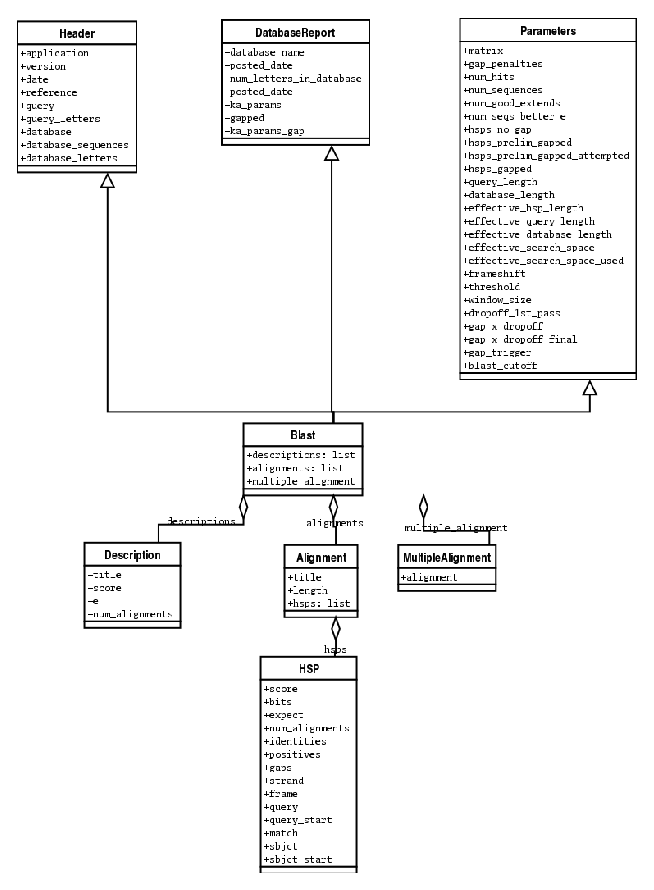
\includegraphics[width=0.8\textwidth]{images/BlastRecord}
\caption{BLAST �Υ�ݡ�����ξ����ɽ�����Ƥ��� Blast Record �Υ��饹��}
\label{fig:blastrecord}
\end{figure}
%\end{latexonly}


\class{PSIBlast} �쥳���ɥ��֥������Ȥ��ɤ����Ƥ��ޤ�����
\program{PSIBlast} �η����֤��Υ��ƥåפ��Ѥ����� \var{rounds}
�򥵥ݡ��Ȥ��Ƥ��ޤ���\class{PSIBlast} �Υ��饹�ޤ��
\ref{fig:psiblastrecord} �˼����ޤ���

%\begin{htmlonly}
%\label{fig:psiblastrecord}
%\imgsrc[width=650, height=750]{images/PSIBlastRecord.png}
%\end{htmlonly}

%\begin{latexonly}
\begin{figure}[htbp]
\centering
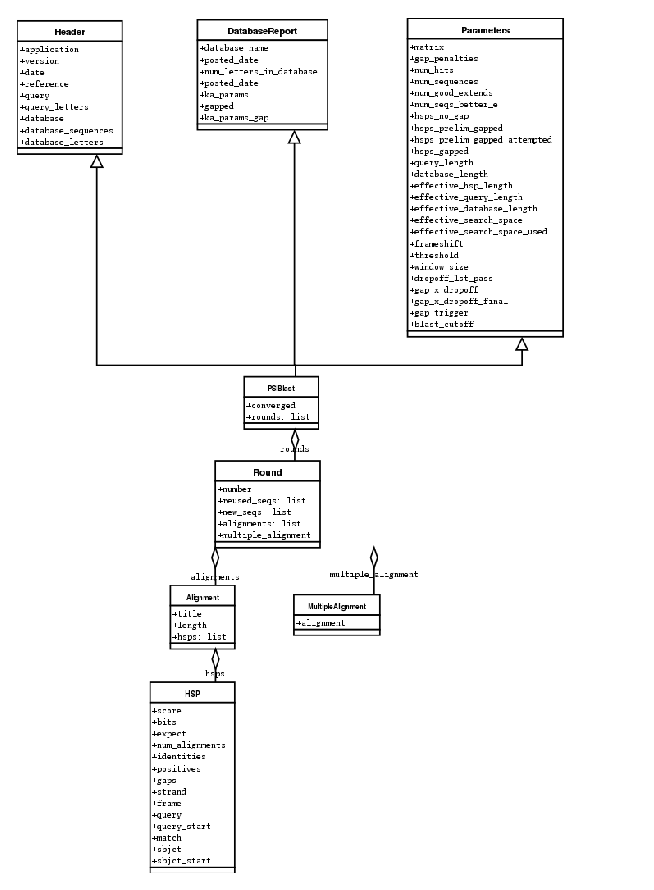
\includegraphics[width=0.8\textwidth]{images/PSIBlastRecord}
\caption{PSIBlast Record ���饹�Υ��饹��}
\label{fig:psiblastrecord}
\end{figure}
%\end{latexonly}

\subsection{��������� BLAST �����餻��}

����򸡺������оݤȤʤ�ǡ����١����򼫺�����ʤ顤��������Ǥ�
\program{BLAST} �μ¹Ԥ��ޤ��ˤ�����ˡ�Ǥ�������饤��Ǥ�
\program{BLAST} ��Ʊ�͡�Biopython �Ǥϥ�����ץȤ����������� 
\program{BLAST} �¹Է�����ƤӽФ��������餷�������ɤ������󶡤��Ƥ��ꡤ
\program{BLAST} �¹Է������󶡤��Ƥ����¿���Υ��ޥ�ɥ饤�󥪥ץ����
�����ƥ��������Ǥ���褦�ˤʤäƤ��ޤ���
�͡��ʥץ�åȥե���������Υ���ѥ���ѤߤΥ�������¹���
\program{BLAST} �ϡ�
\url{ftp://ncbi.nlm.nih.gov/blast/executables/} �Ǽ������ޤ���
�ޤ���NCBI toolbox (\url{ftp://ncbi.nlm.nih.gov/toolbox/}) ����
��ʬ�ǥ���ѥ��뤷�Ƥ�����Ǥ��ޤ���

��������Ǥ�\program{BLAST} �¹Ԥ����뤿��Υ����ɡ��Ȥ�櫓
\function{blastall} ��\function{blastpgp} �Ȥ��ä��ؿ��ϡ�
\module{Bio.Blast.NCBIStandalone} �ˤ���ޤ��������δؿ���
����̾�������ץ������¹Է������б����Ƥ��ޤ���

�����δؿ���Ȥäƥ�������Υǡ����١������Ф���\program{blastall}
��¹Ԥ�����̤��֤����Ƥߤޤ��礦���ޤ���\program{blast} ��¹Ԥ��뤿
���ɬ�פʥѥ������ꤷ�Ƥ����ޤ��礦���ΤäƤ����ͤФʤ�ʤ��Τϡ�
(\program{formatdb} ���Ѱդ��Ƥ������Ϥ���) �����оݤȤ���ǡ����١���
�ؤΥѥ���������������������ä��ե�����ؤΥѥ���������
\program{blastall} �¹Բ�ǽ�����ؤΥѥ����̤�ɬ�פ�����ޤ���

\begin{verbatim}
import os

my_blast_db = os.path.join(os.getcwd(), 'at-est', 'a_cds-10-7.fasta')
my_blast_file = os.path.join(os.getcwd(), 'at-est', 'test_blast',
                             'sorghum_est-test.fasta')
my_blast_exe = os.path.join(os.getcwd(), 'blast', 'blastall')
\end{verbatim}

���ƤΥѥ������ꤷ���Τǡ�\program{blast} ��¹Ԥ��Ʒ�̤���Ф�
�����������ޤ�����������Ԥ�\program{blast} ��¹Ԥ��ޤ�:

\begin{verbatim}
from Bio.Blast import NCBIStandalone

blast_out, error_info = NCBIStandalone.blastall(my_blast_exe, 'blastn',
                                                my_blast_db, my_blast_file)
\end{verbatim}

���������\program{blast} �ץ��������Ф��� Biopython ��
���󥿥ե������ϡ���Ĥ��ͤ��֤��Ƥ��뤳�Ȥ����դ��Ƥ���������
�ǽ������ͤ�\program{blast} �ν��Ϥ��Ф���ϥ�ɥ�ǡ�
��¸������ѡ������Ϥ�����Ǥ��ޤ�������ܤ�����ͤϡ�\program{blast}
���ޥ�ɤ��������뤳�Ȥ����륨�顼���Ϥ�����ޤ���

���顼����μ�갷�������Ǥ����Ȥ����Τϡ����顼��¸�ߤ��ʤ�����
\code{error_info.read()} ��¹Ԥ��褦�Ȥ���ȡ�\function{read}
�ν������֥��å�����Ƥ��ޤä��ͤ��֤��ʤ�����˥�����ץȤ�
��ߤ��Ƥ��ޤ�����Ǥ�����ιͤ��Ǥϡ�\code{blast_out} ��
�֤��줿��̤���Ϥ��Ƥⲿ�������ʤ��ä����ˤΤߥ��顼��
���Ϥ�������ʳ��ξ��ˤϲ��⤻���ۤ��äƤ����Τ������顼��
���ޤ���갷�����֤�����ˡ�Ǥ���

��̤���Ϥ������˥ե��������¸���Ƥ������ȻפäƤ���ʤ顤
���� WWW \program{blast} ����򻲾Ȥ��ơ�\module{copy} �⥸�塼���
�Ȥ����ˤĤ���Ĵ�٤Ƥ������ɤ��Ǥ��礦��

���ơ����Ϥ�������ä��Τǡ����β��Ϥ�Ԥ�ͤФʤ�ޤ���͡�
�Ǥ�����ɤ߿ʤ�ǡ���������Ǽ¹Ԥ���\program{BLAST} �ν��Ϥ���Ϥ���
��ˡ�ˤĤ��ƳؤӤޤ��礦��

\subsection{�������� BLAST �ν��Ϥ���Ϥ���}

�������� \program{BLAST} ������������Ϥϡ�web �١�����\program{BLAST}
�ν��ϤȤϰ�äƤ���Τǡ�\module{Bio.Blast.NCBIStandalone} ���äƤ���
�ѡ�����ȤäƷ�̤�������ޤ���

WWW blast �ξ���Ʊ�� (���Ҥξ���򻲾Ȥ��Ƥ�������)��
�ѡ����˽��Ϥ��Ϥ��ˤϡ��ϥ�ɥ륪�֥������Ȥ���äƤ��ʤ����
�ʤ�ޤ��󡥥ϥ�ɥ륪�֥������Ȥ� \function{readline} �᥽�åɤ�
�������Ƥ��ơ��������������ν�����ԤäƤ���ʤ���Фʤ�ޤ���
���������ϥ�ɥ�����뤿��ˤ褯�Ȥ�������ϡ�\function{blastall}
��\function{blastpgp} �Τ褦�ʡ�Biopython ���󶡤��Ƥ���ؿ���Ȥä�
��������\program{BLAST} ��¹Ԥ��뤫��\program{blast} ��
���ޥ�ɥ饤��ǥ�������˼¹Ԥ��ơ��ʲ��Τ褦�ʥ����ɤ�¹Ԥ��ޤ�:

\begin{verbatim}
blast_out = open('my_file_of_blast_output', 'r')
\end{verbatim}

WWW \program{blast} ��Ʊ���褦�ˡ��̤� Biopython ���ص��ؿ���
�虜�虜�Ȥ�ɬ�פϤ���ޤ���

���ơ��ϥ�ɥ뤬������ä��Τǡ�(�ʸ夳��� \code{blast_out} ��
�Ƥ֤��Ȥˤ��ޤ�) �����Ϥ���Ϥ���������Ǥ��ޤ��������Ϥβ��Ϥ�
�ʲ��Τ褦�ʥ����ɤǹԤ��ޤ�:

\begin{verbatim}
from Bio.Blast import NCBIStandalone

b_parser = NCBIStandalone.BlastParser()
b_record = b_parser.parse(blast_out)
\end{verbatim} 

���Υ����ɤ�¹Ԥ���ȡ�\program{BLAST} ������������ݡ��Ȥ���Ϥ��ơ�
\module{Blast} \class{Record} ���饹 (���Ϥ��Ƥ�����Ϥ�
���Ƥˤ�äơ�\class{Record} ���饹�� Blast �Ѥ� PSIBlast �Ѥ�
�ɤ��餫�ˤʤ�ޤ�) ������������������ǡ�������Ф���褦��
���Ƥ���ޤ����������Ǥϡ�������Ͱʾ�Υ��饤��������Ƥ��Ф���
��ñ�ʥ��ޥ����Ϥ��Ƥߤޤ���


\begin{verbatim}
E_VALUE_THRESH = 0.04
for alignment in b_record.alignments:
    for hsp in alignment.hsps:
        if hsp.expect < E_VALUE_THRESH:
            print '****Alignment****'
            print 'sequence:', alignment.title
            print 'length:', alignment.length
            print 'e value:', hsp.expect
            print hsp.query[0:75] + '...'
            print hsp.match[0:75] + '...'
            print hsp.sbjct[0:75] + '...'
\end{verbatim}

WWW �� �� BLAST �ˤ�������ϲ��ϤˤĤ��Ƥ���򤹤Ǥ��ɤ�Ǥ���С�
�嵭�����ɤ��������������Ƥ�Ʊ�����ȵ��Ť��Ǥ��礦�����餫��
���Ϥ���Ϥ��� \class{Record} ���饹�ˤ����顤��ϸ�����
\program{BLAST} �ν��Ϸ����˴ط��ʤ���갷����ΤǤ���
�ޤä��������餷����

�ְ�ĤΥ쥳���ɤ���ϤǤ���ΤϳΤ��ˤ��������ɡ�����������
�����쥳���ɤ����ä�\program{BLAST} ���ϥե�������ä���ä������͡�
-- ����äƤɤ���ä����������ϤǤ����?�׿��ۤ�̵�ѡ�������
������ˤ���ޤ���


\subsection{BLAST �ν��ϤǤ��äѤ��Υե��������Ϥ���}

����������������������ޤȤ�ˤ��ƥǡ����١��������ơ�
���Ƥ�������Ф��Ƥ褯�Ǥ�����ݡ��Ȥ���Ф���Ȥ������Ǥϡ�
�������� \program{blast} �Ϥ褯�Ǥ��Ƥ��ޤ���
�Ǥ����顤Biopython �ˤϡ��ϼ��Ǥ����ե��������������
Ǻ�ޤ��줺�˲��Ϥ��뵡ǽ������ޤ���

����ʥե�����β��Ϥϡ�blast ���ƥ졼�� (blast iterator)
���Ѥ��ƹԤ��ޤ������ƥ졼����Ȥ���褦�ˤ���ˤϡ��ޤ�
�ѡ��������ꤷ�ơ�blast �ν��ϥ�ݡ��Ȥ���Ϥ��� Blast 
\class{Record} ���֥������Ȥˤ��ޤ�:

\begin{verbatim}
from Bio.Blast import NCBIStandalone

b_parser = NCBIStandalone.BlastParser()
\end{verbatim}

���ˡ������췲�� blast �쥳���ɤ��Ф���ϥ�ɥ뤬�긵�ˤ����
���ꤷ�ơ������ \code{blast_out} �ȸƤ֤��Ȥˤ��ޤ���
�ϥ�ɥ�μ����ˤĤ��Ƥϡ���� blast ���Ϥβ��Ϥ˴ؤ������
�ܤ����Ҥ٤Ƥ��ޤ���

�ѡ�����ϥ�ɥ뤬������ä��Ȥ����ǡ��ʲ��Τ褦�ʥ��ޥ�ɤ�¹�
����С����ƥ졼��������Ǥ��ޤ�:

\begin{verbatim}
b_iterator = NCBIStandalone.Iterator(blast_out, b_parser)
\end{verbatim}

����ܤΥ��ץ����\code{b_parser} �ϥ��ץ����Ǥ���
�ѡ�������ꤷ�ʤ���С����Υ��ƥ졼�������� BLAST ��ݡ��Ȥ�
��İ���֤��Ƥ椭�ޤ���

���ƥ졼����������ä��顤(�ѡ�������������) blast �쥳���ɤ�
\function{next} �Ǽ��Ф��ޤ�:

\begin{verbatim}
b_record = b_iterator.next()
\end{verbatim}

���ƥ졼����\function{next} ��ƤӽФ����Ӥ˿������쥳���ɤ���
�֤��ޤ���
���ơ����Υ쥳�������Τˤ錄�ä�ȿ����� (iteration) ��Ԥ���
����������� blast ����ݡ��Ȥ�����Ǥ��ޤ�:

\begin{verbatim}
while 1:
    b_record = b_iterator.next()

    if b_record is None:
        break

    E_VALUE_THRESH = 0.04
    for alignment in b_record.alignments:
        for hsp in alignment.hsps:
            if hsp.expect < E_VALUE_THRESH:
                print '****Alignment****'
                print 'sequence:', alignment.title
                print 'length:', alignment.length
                print 'e value:', hsp.expect

                if len(hsp.query) > 75:
                    dots = '...'
                else:
                    dots = ''
                
                print hsp.query[0:75] + dots
                print hsp.match[0:75] + dots
                print hsp.sbjct[0:75] + dots
\end{verbatim}

�쥳���ɤ���Ϥ����äƤ��ޤ���\code{b_iterator.next()} ��
\code{None} ���֤����Ȥ����դ��Ƥ�������������ˤ�äơ�
�쥳���ɤ�¸�ߤ��뤫Ĵ�٤ʤ���\keyword{while} �롼�פ�¹Ԥ���С�
��ñ�˥ե��������Τˤ錄�ä�ȿ�������Ǥ��ޤ���

���ƥ졼����Ȥ��ȡ������оݤ���٤˰�ñ�̤Ť��ɤ߹���Τǡ������
blast �쥳���ɤ����������ʤ��˽����Ǥ��ޤ�����Ϥ���
��ǽ��ȤäƤȤ�Ǥ�ʤ��Ф��Ǥ����ե��������������ʤ�
���Ϥ������Ȥ�����ޤ���

\subsection{����ʥե������椫�������ʥ쥳���ɤ�õ��}

�������ƤȤƤ��Բ��˻פ�����ϡ������ BLAST �ե�����򤷤Ф餯��
�ֲ��Ϥ��Ƥ��ơ����θ�ѡ����� \exception{SyntaxError} ����ߤ���
�Ȥ�����ΤǤ�������Ͽ��������Ǥ����Ȥ����Τ⡤
\exception{SyntaxError} ���ѡ���������ʤΤ������뤤�� \program{BLAST}
������ʤΤ���ʬ����ʤ�����Ǥ�������˰������Ȥˡ����顼��̵�뤹��
���Ȥ���Ǥ��ޤ��󡥤Ȥ����Τ⡤�ɤ��Dz��Ϥ����Ԥ����Τ�Ƚ��ʤ��Τǡ�
���顼��̵�뤹��ȥǡ����ν��פʥݥ���Ȥ򸫲ᤴ���Ƥ��ޤ�����
����ʤ�����Ǥ���

���������������򤹤뤿��ˤϤ���äȤ���������ץȤ�񤫤ͤФʤ�ʤ�
�Τ���Ǥ����������� \module{Bio.Blast} �⥸�塼��ˤ�
\class{BlastErrorParser} �����ꡤ��Ȥ������˴�ñ�ˤ��Ƥ���ޤ���
\class{BlastErrorParser} �ϡ��̾�� \class{BlastParser} ��
���ˤ褯���Ƥ��ޤ������ѡ��������Ф���\exception{SyntaxError} 
����­���ơ�������ʬ�Ϥ��褦�Ȼ�ߤ�쥤�䤬�ɲä���Ƥ��ޤ���

���Υѡ����λȤ��������äȸ��Ƥߤޤ��礦 -- �ޤ��������оݤ�
�ե�����ȡ�ȯ����������Υ�ݡ��Ȥ�񤭽Ф�����Υե������������ޤ�:

\begin{verbatim}
import os
 
b_file = os.path.join(os.getcwd(), 'blast_out', 'big_blast.out')
error_file = os.path.join(os.getcwd(), 'blast_out', 'big_blast.problems')
\end{verbatim}

������\class{BlastErrorParser} ��ɬ�פˤʤ�ޤ�:

\begin{verbatim}
from Bio.Blast import NCBIStandalone

error_handle = open(error_file, 'w')

b_error_parser = NCBIStandalone.BlastErrorParser(error_handle)
\end{verbatim}

�ѡ������ϥ�ɥ�򥪥ץ����ΰ����Ȥ��Ƽ�äƤ��뤳�Ȥ�����
���Ƥ����������ϥ�ɥ���Ϥ��ȡ��ѡ�����\exception{SyntaxError}
�����Ф��� \program{blast} �����ƤΥ쥳���ɤ򤳤Υϥ�ɥ��
�񤭽Ф��ޤ����ϥ�ɥ�����ꤷ�ʤ���С����������쥳���ɤ�
��Ͽ����ޤ���

���ơ�\class{BlastErrorParser} ���̾��\program{blast} �ѡ�����
�褦�˻Ȥ��ޤ����Ȥ�櫓��\program{blast} �쥳�������Τˤ錄�ä�
���顼�ѡ�����Ȥäư�ĤŤĥ쥳���ɤ���Ϥ��뤿��˥��ƥ졼����
�������褦�Ȥ��Ƥ⤫�ޤ��ޤ���:

\begin{verbatim}
blast_out = open(b_file)
iterator = NCBIStandalone.Iterator(blast_out, b_error_parser)
\end{verbatim}

���˽Ҥ٤��褦�ˡ����������쥳���ɤϰ��٤˰�ĤŤ��ɤ߽Ф��ޤ���
�����������٤� \program{Blast} �˵������� (���ġ��ѡ������Τ�
�������ʤ�) ���顼����­���ơ�ɬ�פʽ�����Ԥ��ޤ�:

\begin{verbatim}
try:
    next_record = iterator.next()
except NCBIStandalone.LowQualityBlastError, info:
    print "LowQualityBlastError detected in id %s" % info[1]
\end{verbatim}

�����Ǥϡ�\class{BlastErrorParser} �ϰʲ��Τ褦�ʥ��顼�������Ǥ��ޤ�:


\begin{description}
\item [SyntaxError] -- �̾�� \class{BlastParser} ����������Τ�
Ʊ�����顼�ǡ��ѡ���������Υե��������ϤǤ��ʤ����Ȥ˵�������
���顼�Ǥ������Υ��顼���̾�ѡ����ΥХ������ȤäƤ���\program{BLAST}
�ΥС������ȡ��ѡ����������Ǥ���\program{BLAST} �ΥС�������
�԰��פΤ����줫�������Ǥ���

\item [LowQualityBlastError] -- �Ҥɤ��ʼ��ΰ������� 
(�㤨�С�����Ū��ñ��γ˻���Ϣ�ʤ꤫�鹽������Ƥ���褦��û������)
�� BLAST �˳ݤ��褦�Ȥ���ȡ�\program{BLAST} ���������Τ�ޥ�������
���ޤ������Ū�˲����оݤ�����ʤ��ʤäƤ��ޤ����Ȥ�����ޤ���
���ξ�硤���Ƥ����ڤ줿��ݡ��Ȥ����Ϥ��졤�ѡ�����
\exception{SyntaxError} ��Ф��Ƥ��ޤ��ޤ��������������ˤ�
\exception{LowQualityBlastError} �����Ф��ޤ������Υ��顼�ϡ�
�ʲ��Τ褦�ʹ��ܤ򥨥顼����Ȥ����֤��ޤ�:
  \begin{description}
    \item [\code{item[0]}] -- ���顼��å������Ǥ���
    \item [\code{item[1]}] -- ���顼�θ����Ȥʤä����ϥ쥳���ɤ� id 
�Ǥ������ι��ܤϡ����������������Ƥ���쥳���ɤ����Ƶ�Ͽ����
�����������ˤȤƤ�ͭ�ѤǤ���
  \end{description}
\end{description}

��˽Ҥ٤��褦�ˡ����顼��������ȡ�\class{BlastErrorParser} ��
����򵯤����Ƥ���쥳���ɤ�\code{error_handle} �˽񤭽Ф��ޤ���
����\code{error_handle} �����Ƥ�Ĵ�٤ơ���ʬ�λפä��褦�������
�����Ǥ��ޤ���ñ��� \program{blast} ��ݡ��Ȥ�Ȥäƥѡ�����
�ǥХå��Ǥ���Ǥ��⤷��ޤ��󤷡�blast �μ¹Ԥ������Ƥ����꤬
���Ĥ��뤫���Τ�ޤ��󡥤�����ˤ��Ƥ⡤�����餯ͭ�յ����θ���
�ʤ뤳�ȴְ㤤�ʤ��Ǥ�!

\class{BlastErrorParser} ��Ȥ��С������ \program{blast} �ե������
�ǥХå�����������äȳڤˤʤ�Ϥ��Ǥ���


\subsection{PSIBlast ���}

\program{PSIBlast} �򥹥���ץȤ����ñ��ľ�����Ǥ���褦�ˤ���
�ˤϡ�(���饤����ȷ�̤��顤Ŭ�ڤʷ����� align �ե��������Ϥ褦��)
�����ɤ򿧡��Ƚ񤤤Ƥ����ͤФʤ�ޤ��󡥤ޤ��� \program{PSIBlast} ��
�褯Ĵ�٤ơ����ޤ������ˡ��פ��Ĥ�ɬ�פ�����ޤ�...

% 
\section{SWISS-PROT}
\label{sec:swiss-prot}

\subsection{SWISS-PROT �Υ쥳���ɤ����ꤹ��}

SwissProt (\url{http://www.expasy.ch/sprot/sprot-top.html}) ��
����ѥ�����Υǡ����١����ǡ��������ƤϿͼ�ˤ�ä��Խ�����Ƥ��ޤ���
������ץȤ��� SWISS-PROT ����³������ˡ�ȡ�
SWISS-PROT �������֤�����̤�ʸ���Ϥ�����ˡ�򸫤Ƥߤޤ��礦��

�ǽ�ˡ���ʸ���Ϥ����оݤΥǡ����򤤤��Ĥ����Ф��Ƥ���ɬ�פ�����ޤ���
���Υ��륳��������� (chalcone synthase) �����ܤ��Ƥ���Ȥ��ޤ��礦
(�ʤ���̣�����������˵��褦�Ȥ��Ƥ��뤫�� ~\ref{sec:orchids} ��
���Ȥ��Ƥ�������)�����륳��������Ǥϡ���ʪ�Υե�ܥΥ��ɤ���������
�ط����Ƥ��ޤ����ե�ܥΥ��ɤ���ϡ������� UV �ݸ�ޤʤɤ�¿����
�����餷�����ʤ���������ޤ���

SwissProt �Ǹ�����Ԥ��ȡ����륳��������Ǥ˴ؤ�����ͳ��Υ���ѥ���
ID O23729, O23730, O23731 �����Ĥ���Ϥ��Ǥ���
�Ǥϡ�������ץȤ�񤤤ơ������Υ���ѥ��˴ؤ���ǡ��������ꤷ��
�ǡ�����ʸ���Ϥ������򤽤��ʾ������Ф��Ƥߤޤ��礦��

�ޤ��� \module{Bio.WWW.Expasy} �� \function{get_sprot_raw} �Ȥ����ؿ�
��ȤäƤ����Υ쥳���ɤ����ꤷ�ޤ���
���δؿ��ϤȤƤ������餷���� id �����Ϥ���ȡ����̤Υƥ����ȷ�����
�쥳���ɤ��֤��ޤ� (html �Ƕ�ϫ���ʤ��Ƥ��ߤޤ�!)��

��Ū�� 3 �ĤΥ쥳���ɤ������줿�顤1 �Ĥ��礭��ʸ����Ȥ��ƤޤȤᡤ
�Ĥ��ˤ���ʸ������ᤵ���ޤ������񤤤����Ȥ��Τ�Τ����ʲ��˼���
�����ɤǼ¸��Ǥ��ޤ�:

\begin{verbatim}
from Bio.WWW import ExPASy

ids = ['O23729', 'O23730', 'O23731']

all_results = ''
for id in ids:
    results = ExPASy.get_sprot_raw(id)
    all_results = all_results + results.read()
\end{verbatim}

���ơ�Expasy �Ǥθ�����̤����ꤷ���Τǡ����η�̤�ʸ���Ϥ��ƶ�̣��
���������Ф������������ޤ�����¾��¿���Υѡ�����Ʊ���褦�ˡ�
���ƥ졼���ȥѡ����򥻥åȥ��åפ��ޤ����������Ѥ���ѡ����� SwissProt
�ե������ʸ���Ϥ��ƥ쥳���ɥ��֥������Ȥ��Ѵ����ޤ����쥳���ɤǤϡ�
��̣���оݤȤʤ�°������ (feature) �����֥������Ȥ�°���ˤʤäƤ��ޤ�:

\begin{verbatim}
from Bio.SwissProt import SProt
from Bio import File

s_parser = SProt.RecordParser()
s_iterator = SProt.Iterator(File.StringHandle(all_results), s_parser)
\end{verbatim}

�ѡ����ǹ�ʸ���Ϥ�Ԥ����ˡ�ʸ����� \var{all_results} ��ϥ�ɥ�
(handle) ���Ѵ����Ƥ��뤳�Ȥ����դ��Ƥ������������ƥ졼�������ϥǡ���
���ԤŤ��ɤ߹����褦�ˤ��뤿��ˡ����ƥ졼���ˤϥϥ�ɥ���Ϥ��ͤ�
�ʤ�ޤ���
\module{Bio.File} �⥸�塼��ˤϡ�\function{StringHandle} �Ȥ����褯
�Ǥ��������ʴؿ������ꡤʸ�����ϥ�ɥ���Ѵ����Ƥ���ޤ���
�����餷��! ����ǡ��������Ф�������������ޤ�����

�������Ф�����ˡ����ƥ졼����Ȥäơ����ƤΥ쥳���ɤ���
���ɤ�ޤ��������Ǥϡ��ƥ쥳���ɤ��Ф��ơ�ñ�ˤ���äȤ������ޥ�����
ɽ�����ޤ��礦:

\begin{verbatim}
while 1:
    cur_record = s_iterator.next()

    if cur_record is None:
        break

    print "description:", cur_record.description
    for ref in cur_record.references:
        print "authors:", ref.authors
        print "title:", ref.title

    print "classification:", cur_record.organism_classification
    print
\end{verbatim}

��Υ����ɤϡ��ʲ��Τ褦�ʥ��ޥ����Ϥ��ޤ�:

\begin{verbatim}
description: CHALCONE SYNTHASE 8 (EC 2.3.1.74) (NARINGENIN-CHALCONE SYNTHASE 8)
authors: Liew C.F., Lim S.H., Loh C.S., Goh C.J.;
title: "Molecular cloning and sequence analysis of chalcone synthase cDNAs of
Bromheadia finlaysoniana.";
classification: ['Eukaryota', 'Viridiplantae', 'Embryophyta', 'Tracheophyta', 
'Spermatophyta', 'Magnoliophyta', 'Liliopsida', 'Asparagales', 'Orchidaceae', 
'Bromheadia']
\end{verbatim}

SwissProt �쥳���ɤ���¾�ξ������Ф�������С�Ʊ���褦�˴�ñ��
�Ԥ��ޤ���

\section{PubMed}
\label{sec:pub-med}

\subsection{PubMed �˥��������������}

���ʬ��뤤�ϥҥȤ˴ؿ�������ʤ� (���Ȥ������Ǥʤ��Ƥ⡤�ۤȤ�ɤ�
���!)��PubMed (\url{http://www.ncbi.nlm.nih.gov/PubMed/}) ��������
�����ͥ�줿���󸻤ˤʤ�Ǥ��礦���Ǥ����顤¾�ξ����Ʊ���褦�ˡ������Ǥ� 
Python ������ץȤ�Ȥäƾ����������ƻȤ���褦�ˤʤꤿ���Ǥ��͡�

Biopython ���Ѥ��� PubMed �˥����������Τϴ�ñ�Ǥ������˴ط��Τ���
���٤Ƥ�ʸ�� ID (article id) ����������С��ʲ��Τ��ä� 3 �ԤΥ�����
����ɬ�פ���ޤ���:

\begin{verbatim}
from Bio import PubMed

search_term = 'orchid'
orchid_ids = PubMed.search_for(search_term)
\end{verbatim}

���Υ����ɤϡ����˴ؤ��뤹�٤Ƥ�ʸ�� ID �� python �Υꥹ�ȤȤ���
�֤��ޤ�:


\begin{verbatim}
['11070358', '11064040', '11028023', '10947239', '10938351', '10936520', 
'10905611', '10899814', '10856762', '10854740', '10758893', '10716342', 
...
\end{verbatim}

���� ID �ꥹ�Ȥ������顤�ƥ쥳���ɤ������������ϴ�λ�Ǥ��������
�ʤߤޤ��礦��

\subsection{PubMed �Υ쥳���ɤ����ꤹ��}

����Ǥϡ���Ϣ�� ID �����������ˡ���������ޤ�����
ID �����ꤷ���顤���ϳ� ID �˴ط��Τ��� MEDLINE �Υ쥳���ɤ����ꤷ�ơ�
��������������Ф������ȹͤ���Ǥ��礦��

PubMed ����쥳���ɤ���Ф��륤�󥿡��ե������ϡ�Python �ץ�����ޡ���
�ȤäƤϤȤƤ�ľ��Ū�ʤϤ� -- Python �ˤ����뼭�񷿤Υ�ǥ벽 -- �Ǥ���
���Υ��󥿡��ե������򥻥åȥ��åפ���ˤϡ�PubMed �������������̤�
��ʸ���Ϥ��뤿��Υѡ�����ɬ�פǤ����ʲ��Υ����ɤǡ����ƤΥ��åȥ��å�
��Ԥ��ޤ�:

\begin{verbatim}
from Bio import PubMed
from Bio import Medline

rec_parser = Medline.RecordParser()
medline_dict = PubMed.Dictionary(parser = rec_parser)
\end{verbatim}

�����ǹԤä��Τϡ�����饤���ʥ��֥������Ȥ� \var{medline_dict} �κ���
�Ǥ���ʸ�����������ˤϡ�\code{medline_dict[id_to_get]} �Τ褦�ˤ���
�����������ޤ�����������Ԥ��ȡ� PubMed ����³����õ���Ƥ���ʸ����
���Ĥ���ʸ�������ʸ���Ϥ��ƥ쥳���ɥ��֥������Ȥ��Ѵ������֤��ޤ���
�ʤ�Ƹ�����Ǥ��礦! 


���ơ����������餷�����񥪥֥������Ȥ�ɤ��Ȥ��С����� ID ���餢�����
����ϤǤ��뤫���Ƥߤޤ��礦��ɬ�פʺ�Ȥϡ�ñ�˼긵�� ID (���������
���� \var{orchid_ids} �ˤˤ錄�äƥ롼�פ�����̣���оݤȤʤ�����ɽ��
��������Ǥ�:


\begin{verbatim}
for id in orchid_ids[0:5]:
    cur_record = medline_dict[id]
    print 'title:', string.rstrip(cur_record.title)
    print 'authors:', cur_record.authors
    print 'source:', string.strip(cur_record.source)
    print
\end{verbatim}

��Υ����ɤ��Ф�����Ϥϰʲ��Τ褦�ˤʤ�ޤ���

\begin{verbatim}
title: Sex pheromone mimicry in the early spider orchid (ophrys sphegodes):
patterns of hydrocarbons as the key mechanism for pollination by sexual
deception [In Process Citation]
authors: ['Schiestl FP', 'Ayasse M', 'Paulus HF', 'Lofstedt C', 'Hansson BS', 
'Ibarra F', 'Francke W']
source: J Comp Physiol [A] 2000 Jun;186(6):567-74
\end{verbatim}

��ɮ���٤��ϡ�����̾�Υꥹ�ȤǤ��������ɸ��� Python �ꥹ�ȷ��Ȥ���
�֤���Ƥ��ޤ����������뤳�Ȥǡ�Python ��ɸ��ġ����Ȥä�������
����������Ǥ��ޤ����㤨�С��ʲ��Τ褦�ʥ����ɤ�Ȥ��С���Ϣ�Υ���ȥ�
���Τˤ錄�äƥ롼�פ��ơ���������Ԥ�õ���Ф��ޤ�:


\begin{verbatim}
search_author = 'Waits T'

for id in our_id_list:
    cur_record = medline_dict[id]
    
    if search_author in cur_record.authors:
        print "Author %s found: %s" % (search_author,
                                       string.strip(cur_record.source))
\end{verbatim} 

PubMed �� Medline �Υ��󥿡��ե����������Ϥ����褯����Ƥ��ޤ� -- 
������ɤ�ǡ����äȤ��Υ��󥿥ե������ΰ��ϤȻȤ�����褯���򤷤�
��館�����ȤǤ��礦��

\section{GenBank}


GenBank �쥳���ɷ����ϡ����������˴ؤ���°������ (feature)��
����¾��Ϣ��������ξ����Ͽ������ˡ�Ȥ��ƹ����Ȥ��Ƥ��ޤ���
���η����ϡ�NCBI �Υǡ����١��� (\url{http://www.ncbi.nih.gov/}) 
�����������뤿����ɤ����ʤǤ⤢��ޤ���


\subsection{GenBank �Υ���ȥ�� NCBI �������ꤹ��}

\module{Bio.GenBank} �饤�֥�� �ΤȤƤ���Ũ�ʵ�ǽ�ϡ�����ȥ��
GenBank ���鼫ưŪ�˼����Ǥ���Ȥ����Ȥ����Ǥ���
����ϡ������κ�Ȥ�ư������褦�ʥ�����ץȤ�񤯾�ǤȤƤ�
�����Ǥ����������Ǥϡ�NCBI �ǡ����١����˥����������������������
����쥳���ɤ����ꤹ����ˡ�򼨤��ޤ���

�ޤ��ϥ������������ơ����Ф������쥳���ɤ��Ф��� ID �򸡺�
���ޤ��礦�������Ǥϡ���Τ����������\emph{�����掠�ܥƥ� (Opuntia)}
����˼�äơʤʤ��ʤ�䤬���椷�Ƥ��뤫��Ǥ��ˡ�����äȤ���������
�¹Ԥ��Ƥߤޤ��礦���ʲ��Υ����ɤ�Ȥ��С������å�������Ԥäơ�
���ƤΥ쥳���ɤ��б����� GI (GenBank ���̻�) ������Ǥ��ޤ�:

\begin{verbatim}
from Bio import GenBank

gi_list = GenBank.search_for("Opuntia AND rpl16")
\end{verbatim}

\var{gi_list} �ˤϡ�������˰��פ������٤Ƥ� GenBank ���̻Ҥ���ʤ�
�ꥹ�Ȥˤʤ�ޤ�:

\begin{verbatim}
['6273291', '6273290', '6273289', '6273287', '6273286', '6273285', '6273284']
\end{verbatim}

GI ������Ǥ����Τǡ��� ID ��ȤäƼ��񥤥󥿥ե�������𤷤� NCBI 
�ǡ����١����˥��������Ǥ��ޤ����㤨�С��ǽ�� GI ���Ф�������
��Ф���ʤ顤�ޤ� NCBI �˥����������뼭�񥪥֥������Ȥ���ʤ��Ƥ�
�ʤ�ޤ���:


\begin{verbatim}
ncbi_dict = GenBank.NCBIDictionary()
\end{verbatim}

���񥪥֥������Ȥ��ä��顤���Τ褦�˾������Ф��Ƥߤޤ��礦:

\begin{verbatim}
gb_record = ncbi_dict[gi_list[0]]
\end{verbatim}

������Ǥϡ�\var{gb_record} �� GenBank �����Υ쥳���ɤˤʤ�Ϥ��Ǥ�:

\begin{verbatim}
LOCUS       AF191665      902 bp    DNA             PLN       07-NOV-1999
DEFINITION  Opuntia marenae rpl16 gene; chloroplast gene for chloroplast
            product, partial intron sequence.
ACCESSION   AF191665
VERSION     AF191665.1  GI:6273291
...
\end{verbatim}

������Ǥϡ�ñ�����Υ쥳���ɤ����ꤷ�������Ǥ��������Υ쥳���ɤ�
ľ�ܥѡ������Ϥ��ƹ�ʸ���Ϥ������쥳���ɤ��Ѵ����뤳�Ȥ����ޤ���
�㤨�С� GenBank �ե����뤫����Ф��� \class{SeqFeature}
���֥������Ȥ� \class{SeqRecord} ���֥������Ȥ��ᤷ������С�
�ޤ�\module{GenBank} �� \class{FeatureParser} �Ǽ��񥪥֥������Ȥ�
��������ɬ�פ�����ޤ�:

\begin{verbatim}
record_parser = GenBank.FeatureParser()
ncbi_dict = GenBank.NCBIDictionary(parser = record_parser)
\end{verbatim}

����ǡ��쥳���ɤ���Ф���С��ǤΥƥ����ȷ����Υ쥳���ɤ�
����� \class{SeqRecord} ���֥������Ȥˤʤ�ޤ�:

\begin{verbatim}
>>> gb_seqrecord = ncbi_dict[gi_list[0]]
>>> print gb_seqrecord
<Bio.SeqRecord.SeqRecord instance at 0x102f9404>
\end{verbatim}

GenBank ����ɤ�ʷ������Ѵ��Ǥ��뤫�ˤĤ��Ƥξܺ٤ϡ�
\ref{sec:gb-parsing} ��򻲾Ȥ��Ƥ���������

����������ưŪ�������̼�����ǽ��Ȥ��ȡ����Ȥ���Ϥ뤫��ͭ���ˤ�
��ޤ������ξ塤������ǽ�ˤϰ�����֤��Ȥ˼�����Ԥ� time-delay �Τ褦
����Ũ�ʵ�ǽ���Ȥ߹��ޤ�Ƥ��ơ����ˤʥ��������ˤ�ä� NCBI ���ܤ餻��
����������֥��å������褦�ʤ��Ȥ��ʤ��褦�ˤ��Ƥ��ޤ���

\subsection{GenBank �쥳���ɤ��᤹��}
\label{sec:gb-parsing}

GenBank �ե�����������餷���Ǥ��Ƥ��ơ���������ξ��󤬤��������
��������ǡ��ºݤˤϰ���ˤۤ�ξ����ξ��󤷤����Ф������ʤ�����
����ޤ��󡥤���������Ȥθ��Ȥʤ�Τϡ��ǡ����򤤤��˹�ʸ���Ϥ��뤫��
����
Biopython �Ǥ�ʣ���� GenBank �ѡ������󶡤��Ƥ��ơ�����������Ȥ�
�Ԥ���Ǽ�����Ǥ���褦�ˤ��Ƥ��ޤ�������ޤǤΤȤ�����
\module{GenBank} �Ǥϰʲ��Υѡ������󶡤��Ƥ��ޤ�:


\begin{description}

\item [RecordParser] ���Υѡ������ǤΥ쥳���ɤ�ʸ���Ϥ��ơ� GenBank 
��ͭ�Υ쥳���ɥ��֥������ȷ������Ѵ����ޤ������Υ��֥������ȤǤ�
������ǤΥ쥳���ɤ����˶ᤤ��ǥ�ǰ����Τǡ�ñ�� GenBank ��
�ġ��Υ쥳���ɼ��Τ˶�̣��������ˤϤ��Υѡ�����Ȥ��Τ��褤�Ǥ��礦��

\item [FeatureParser] ���Υѡ������ǤΥ쥳���ɤ�\class{SeqRecord} 
���֥������Ȥ��Ѵ����ޤ���\class{SeqRecord} ���֥������ȤǤϡ�
���Ƥ�°���ơ��֥����\class{SeqFeatures} ��ɽ������Ƥ��ޤ�
(�����Υ��֥������ȤˤĤ��Ƥξܺ٤� \ref{sec:advanced-seq} ��
���Ȥ��Ƥ�������)�����ɸ��Ū�ʷ����Ǿ�������ꤷ�������ˤ�
������Υѡ�����Ȥ��Τ��褤�Ǥ��礦��

\end{description}

�ɤ������ˡ��Ȥ�ˤ��衤���������Υѡ����κǤ����Ū�ʻȤ����ϡ�
���ƥ졼����������ơ�GenBank �쥳���ɤ����ä��ե������ѡ�������
�Ȥ�����Τˤʤ�ޤ������κ�Ȥϡ�¾�Υǡ��������Ǥν�����ˡ������
���Ƥ��ơ��㤨�аʲ��Τ褦�ʥ����ɤˤʤ�ޤ�:


\begin{verbatim}
from Bio import GenBank

gb_file = "my_file.gb"
gb_handle = open(gb_file, 'r')

feature_parser = GenBank.FeatureParser()

gb_iterator = GenBank.Iterator(gb_handle, feature_parser)

while 1:
   cur_record = gb_iterator.next()

   if cur_record is None:
       break

   # now do something with the record
   print cur_record.seq
\end{verbatim}

���Υ����ɤǤϡ�ñ�� GenBank �ե�������Ϥä�ȿ��������Ԥ���
�쥳���ɤ��Ȥ˹�ʸ���Ϥ�Ԥä� SeqRecord �� SeqFeature ���֥������Ȥ�
�Ѵ��������Υ쥳���ɤ������ɽ�� \class{Seq} ���֥������Ȥ�
���Ϥ��ޤ���

¾�η�����Ʊ�͡�GenBank �쥳���ɤ򰷤��ġ��뤬�������󤢤�ޤ���
�����Υġ����Ȥ��� GenBank ��ȤäƤ�ꤿ�����Ȥϲ��Ǥ�Ǥ���
�Ϥ��Ǥ���


\subsection{����� GenBank �ǡ����١������������}

��ʬ�ѤθĿ�Ū�� GenBank �ǡ����١�����������ơ����񥪥֥������Ȥ�
�褦�˥��������Ǥ���Ȥ����ȤƤ������餷����ǽ������ޤ���
(����������餷��������ʵ�ǽ�Ǥ����Ȥ����Τϡ����Υ��������
�ǡ����١����ˤ⡤BioCorba ��Ȥäƥͥåȥ���ۤ��˥�������
�Ǥ��뤫��Ǥ� -- �ܺ٤� BioCorba �Υɥ�����Ȥ򻲾Ȥ��Ƥ�������)

��������ʥǡ����١����κ����Ǥϡ��ޤ�����ǥ����ե������������ơ�
�ե�������γƥ쥳���ɤ����᤯���������Ǥ���褦�ˤ��ޤ���
�����Ԥ��ˤϡ�\function{index_file} �ؿ���Ȥ��ޤ�:

\begin{verbatim}
>>> from Bio import GenBank
>>> dict_file = 'cor6_6.gb'
>>> index_file = 'cor6_6.idx'
>>> GenBank.index_file(dict_file, index_file)
\end{verbatim}

���κ�Ȥǡ� \file{my_index_file.idx} �Ȥ���̾���Υե����뤬����
����ޤ������ơ����Υ���ǥ�����Ȥ��С��ġ��Υ쥳���ɤ˥�������
�Ǥ���褦�ʼ��񥪥֥������Ȥ�����Ǥ��ޤ���
\class{Iterator} �� \class{NCBIDictionary} ���󥿥ե������Τ褦�ˡ�
�ǤΥ쥳���ɤ��ᤷ���ꡤ���񥪥֥������Ȥ�ѡ������Ϥ��ơ��쥳���ɤ�
�֤��������Ƥ�ʸ���Ϥ�������Ǥ��ޤ���
���ξ�硤�쥳���ɤ�������ˤ� \class{FeatureParser} ���Ϥ��Ƥ�����
���θ�� \class{SeqRecord} ���֥������Ȥ�������ޤ���

����ν����ϴ�ñ�ǡ��ʲ��� 1 �Ԥ����Ǥ�:

\begin{verbatim}
>>> gb_dict = GenBank.Dictionary(index_file, GenBank.FeatureParser())
\end{verbatim}

����ǡ�Genbank �Υǡ����򼭽����˰�����褦�ˤʤ�ޤ�����
�㤨��:

\begin{verbatim}
>>> len(gb_dict)
7
>>> gb_dict.keys()
['L31939', 'AJ237582', 'X62281', 'AF297471', 'M81224', 'X55053']
\end{verbatim}

�Ǹ�ˡ�ź��ɽ�� (subscripting) �ǥ��֥������Ȥ���Ф��ޤ�: 

\begin{verbatim}
>>> gb_dict['AJ237582']
<Bio.SeqRecord.SeqRecord instance at 0x102fdd8c>
\end{verbatim}
\section{���饤����Ȳ��Ϥΰ���}

��������󷲤��Ф��ƥ��饤����Ȥ�ݤ�����ȡ��ȤƤ������ʤ��Ȥ�
�褯����ޤ�����ԤϤ����褯�Ȥäơ���äĤ�Ū������֤δ�Ϣ����
Ĵ�٤��ꤷ�ޤ������äơ����饤����Ȥ�ݤ��ơ����η�̤����䤹��
���֥������Ȥ��֤��褦�� Python ������ץȤ򤹤Ф䤯�񤭾夲�����
�����ΤϤȤƤ������餷�����ȤʤΤǤ���Biopython �ˤ����륢�饤�����
��Ϣ�Υ����ɤϡ�Python ��٥뤫�饢�饤����Ȳ��ϥץ������˥�������
�Ǥ���褦�ˤ���������ץȾ夫������ᤤ���饤����Ȳ��Ϥ��ǽ��
���뤿��Τ�ΤǤ���

\subsection{clustalw}
\label{sec:align-clustal}

\program{clustalx}
(\url{http://www-igbmc.u-strasbg.fr/BioInfo/ClustalX/Top.html}) 
�ϡ��ޥ���ץ륢�饤����Ȥ�Ԥ������ͥ�줿�ץ������Ǥ���
Biopython �Ǥϡ�\program{clustalx} ���������� clustal �����Υ��饤����Ⱦ���
(�̾�ϳ�ĥ�� \file{*.aln} ���Ĥ��Ƥ��ޤ�) �˥����������뤿���
��ˡ���󶡤��Ƥ��ޤ����ޤ���\program{clustalx} �Υ��ޥ�ɥ饤���ǤǤ���
\program{clustalw} �ؤΥ����������ʤ��󶡤��Ƥ��ޤ���

\program{clustalw} �Ȥ��Ȥ��Ԥ���Ǥϡ��ޤ��ǽ�Υ��ƥåפȤ��ơ�
�ץ��������Ϥ����ޥ�ɥ饤����������ꤷ�ޤ��� \program{clustalw}
 �ˤ������
���Υ��ޥ�ɥ饤�󥪥ץ���󤬤��ꡤ��������Υѥ�᥿�����ꤹ�뤳�Ȥ�
�ʤ�С�����ʥ��ޥ�ɥ饤������Ϥˤ���˰���Ƥ��ޤ��Ǥ��礦��
���ޥ�ɥ饤�󥯥饹 (command line class) �Ǥϡ�����Ǥ���
���ޥ�ɥ饤�󥪥ץ����򥯥饹��°���Ȥ��ư������Ȥǡ����ޥ�ɥ饤��
���ǥ벽���Ƥ��ޤ�������Υѥ�᥿�����ꤹ�뤿����ص��ؿ���
�����Ĥ����ꡤ�ѥ�᥿����ˤ�����륨�顼�򸡽ФǤ���褦��
�ʤäƤ��ޤ���

\program{clustalw} �ˤ��ޥ���ץ륢�饤����Ȥ�¹Ԥ��뤿���
���ޥ�ɥ饤�󥪥֥������Ȥ��������ˤϡ��ʲ��Τ褦�ˤ��ޤ�:

\begin{verbatim}
import os
from Bio.Clustalw import MultipleAlignCL

cline = MultipleAlignCL(os.path.join(os.curdir, 'opuntia.fasta'))
cline.set_output('test.aln')
\end{verbatim}

�ޤ���\class{MultipleAlignCL} �� import ���ޤ������Υ��饹��
\program{clustalw} �ˤ��ޥ���ץ륢�饤����Ȥμ¹Ԥ��ǥ벽
���Ƥ��ޤ���
���ˡ����Υ��ޥ�ɥ饤�󥯥饹���������ޤ������κݡ�
���饤����Ȥ��оݤˤ��� FASTA �����Υե����������Ȥ���
���ꤷ�ޤ���
������ؿ��ˤϡ����ץ�������������Ȥ��ơ�\program{clustalw}
�μ¹ԥե����뤬����������Ǥ��ޤ����ǥե���ȤǤϡ�
\program{clustalw} ��\envvar{PATH} ��Τɤ����ˤ���Ȳ��ꤷ�ơ�
���ޥ�ɥ饤�󥪥֥������Ȥ�ñ�� \code{'clastalw'} �Ȥ���̾����
�ץ�������ƤӽФ��ޤ���

���ιԤǤϡ���̤ν������ե����� \file{test.aln} �����ꤷ�Ƥ��ޤ���
\class{MultipleAlignCL} ���֥������Ȥˤ�¾�ˤ⤿������Υѥ�᥿
�����ꡤ���Ϥη��������󥮥�åפΥ����ȤȤ��ä������Ԥ��ޤ���

���ޥ�ɥ饤������Ƥϡ�\class{MultipleAlignCL} ��\function{__str__} 
�᥽�åɤ�ƤӽФ�������������ɤ�ޤ����ºݤˤϡ�\code{str(cline)}
�Ȥ����ꡤñ�� \code{print cline} �Ȥ��������ɽ������ޤ���
�����Ǥϡ��ʲ��Τ褦�ʽ��Ϥˤʤ�Ϥ��Ǥ�:

\begin{verbatim}
clustalw ./opuntia.fasta -OUTFILE=test.aln
\end{verbatim}

���ơ���ñ�ʥ��ޥ�ɥ饤�������Ǥ����Τǡ����Υ��ޥ�ɥ饤���
�¹Ԥ��Ʒ�̤���ޤȤᡤ�����Ǥ���褦�ˤ��ޤ��礦��
�������ϡ�\class{Clastalw} ��\function{do_alignment} ��Ȥä�
�ʲ��Τ褦�˹Ԥ��ޤ�:

\begin{verbatim}
from Bio import Clustalw

alignment = Clustalw.do_alignment(cline)
\end{verbatim}

���¹Ԥ���ȡ�Biopython ����ۤ����ꤷ�����ޥ�ɥ饤���¹Ԥ��ơ�
����Υѥ�᥿�� \program{clustalw} �����餻�ޤ�������
\program{clustalw} ����ν��Ϥ�����ߡ�Biopython �����ϤǤ���
���� (���ߤΤȤ��� clustal �����Τ�) �Ǥ���С����Ϥ�Ԥäơ�
Ŭ�ڤʷ��Υ��饤����ȥ��֥������Ȥˤ����֤��ޤ��������Ǥϡ�
��̤�ǥե���Ȥ� clustal �����ˤ��Ƥ���Τǡ�����ͤΥ��֥�������
\code{alignment} ���֥������Ȥ� \class{ClustalAlignment} ���ˤʤ�ޤ���

\code{alignment} ���֥������Ȥ������顤�㤨�Х��饤��������
���Ƥ�������Ф���\class{seq_record} ���֥������Ȥ�����Ȥ��ä�
�褦�ʽ�����Ԥ��ޤ�:

\begin{verbatim}
all_records = alignment.get_all_seqs()

print 'description:', all_records[0].description
print 'sequence:', all_records[0].seq
\end{verbatim}

��Υ����ɤ�¹Ԥ���ȡ����饤����Ȥκǽ�����󥪥֥������Ȥ�
�Ф������� (description) �����󥪥֥������Ȥ���Ϥ��ޤ�:

\begin{verbatim}
description: gi|6273285|gb|AF191659.1|AF191
sequence: Seq('TATACATTAAAGAAGGGGGATGCGGATAAATGGAAAGGCGAAAGAAAGAAAAAAATGAAT 
...', IUPACAmbiguousDNA())
\end{verbatim}

���饤����Ȥκ���Ĺ��׻��Ǥ��ޤ�:

\begin{verbatim}
length = alignment.get_alignment_length()
\end{verbatim}

���饤����ȥ��֥������Ȥ򥪥ꥸ�ʥ�η����ǽ��Ϥ�������С�
ñ�� \function{__str__} �˥���������������Ǥ����Ĥޤꡤ
\code{print alignment} ��¹Ԥ�������Ǥ��ޤ��ޤ���:


\begin{verbatim}
CLUSTAL X (1.81) multiple sequence alignment


gi|6273285|gb|AF191659.1|AF191      TATACATTAAAGAAGGGGGATGCGGATAAATGGAAAGGCGAAAGAAAGAA
gi|6273284|gb|AF191658.1|AF191      TATACATTAAAGAAGGGGGATGCGGATAAATGGAAAGGCGAAAGAAAGAA
...
\end{verbatim}

��������С����ꥸ�ʥ�ξ���˼��ä��뤳�Ȥʤ������饤����ȷ�̤�
�ե�����˴�ñ�˽��᤻�ޤ���

���饤����ȷ�̤�Ȥä�¾�ˤ⤤�������ʤ��Ȥ򤷤Ƥߤ�����С�
���饤����ȷ�̤�\class{SummaryInfo} ���֥�������
�Τ褦�ʥ��饤����Ⱦ����������֥������Ȥ��Ϥ��Τ��٥��ȤǤ���
����ˤĤ��Ƥ�\ref{sec:summary-info} ����������ޤ���

\subsection{���ޥ����λ���}
\label{sec:summary-info}

���饤����ȷ�̤������顤���Ϥ�������������Ф����Ȥ���
�Ϥ��Ǥ��͡�Biopython �Ǥϡ����륢�饤����Ⱦ���˴ؤ������Ƥξ����
��������褦�ʰ�Ϣ�δؿ������ƥ��饤����ȥ��֥������Ȥ˻�������
����ˡ�����������ǽ�򥢥饤����ȥ��֥������Ȥ���������̤�
���饹��ʬΥ���褦�Ȼ�ߤƤ��ޤ���

���饤����ȥ��֥������Ȥ��饵�ޥ����򻻽Ф�������ϤȤƤ�
��ñ�Ǥ����㤨�С�\code{alignment} �Ȥ���̾���Υ��֥������Ȥ�
����Ȥ��ޤ��礦�����ޥ����򻻽Ф��륪�֥������Ȥ�������ɬ�פʤΤ�
��������Ǥ�:

\begin{verbatim}
from Bio.Align import AlignInfo
summary_align = AlignInfo.SummaryInfo(alignment)
\end{verbatim}

\code{summary_align} �ϤȤƤ������ʥ��֥������Ȥǡ��ʲ��Τ褦��
����������������ԤäƤ���ޤ�:

\begin{enumerate}
  \item ��ñ�ʥ��󥻥󥵥�����η׻� -- \ref{sec:consensus} �Ỳ��
  \item �����ð�Ū���������� (position specific score matrix) �η׻�
    -- \ref{sec:pssm} �Ỳ��
  \item �����̤η׻� -- \ref{sec:getting-info-content} �Ỳ��
  \item �Ĵ��ִ���������� -- ���ε�ǽ��
    �Ȥä��ִ���������ˡ�ξܺ٤�\ref{sec:sub-matrix} �Ỳ��
\end{enumerate}

\subsection{��ñ�ʥ��󥻥󥵥�����η׻�}
\label{sec:consensus}

\ref{sec:summary-info} ��Dz��⤵��Ƥ���\class{SummaryInfo} 
���֥������ȤǤϡ����饤����Ȥˤ������ñ�ʥ��󥻥󥵥�����
��׻����뵡ǽ���󶡤��Ƥ��ޤ���\code{summary_align} �Ȥ���̾����
\class{SummaryInfo} ���֥������Ȥ����Ƥ���Ȥ��ơ����󥻥󥵥������
�׻��ϰʲ��Τ褦�ˤ��ƹԤ��ޤ�:


\begin{verbatim}
consensus = summary_align.dumb_consensus()
\end{verbatim}

̾������������褦�ˡ����δؿ����Ԥ��Τ������˴�ñ�ʥ��󥻥󥵥��׻�
�ǡ����󥻥󥵥���ʬ�γ��������ƤλĴ��ȹ礷���Ǥⶦ�����ι⤤�Ĵ��
�ͤ����� (�ǥե���Ȥ� 0.3) ���⤤�ͤ���ľ��ˡ����λĴ��
���󥻥󥵥�������ɲä��ޤ���
���ͤ�ã���ʤ���С�ۣ��ʻĴ��ɽ��ʸ���򥳥󥻥󥵥�������ɲ�
���ޤ�������ͤΥ��󥻥󥵥������ \class{Seq} ���֥������Ȥǡ�����
����ե��٥åȤϥ��󥻥󥵥��������Ȥ����������󤫤��¬���ޤ���
���äơ�\code{print consensus} ��¹Ԥ���ȡ��ʲ��Τ褦�ʽ��Ϥ�
�ʤ�Ϥ��Ǥ�:


\begin{verbatim}
consensus Seq('TATACATNAAAGNAGGGGGATGCGGATAAATGGAAAGGCGAAAGAAAGAAAAAAATGAAT 
...', IUPACAmbiguousDNA())
\end{verbatim} 

���ץ����Υѥ�᥿���Ϥ��ȡ�\function{dumb_consensus} ��ư���
Ĵ���Ǥ��ޤ�:

\begin{description}
\item[����] ���󥻥󥵥�����γ����ˤ����ơ�����λĴ�򥳥󥻥󥵥�
�Ȥ��ƺ��Ѥ��뤿���ɬ�פʻĴ�ζ������Ǥ����ǥե���Ȥ� 0.7 �Ǥ���

\item[ۣ��ʻĴ��ɽ��ʸ��] ۣ��ʻĴ��ɽ���˻Ȥ���ʸ���Ǥ���
�ǥե���Ȥ� \code{'N'} �Ǥ���

\item[���󥻥󥵥�����Υ���ե��٥å�] ���󥻥󥵥�����˻Ȥ�
����ե��٥åȤǤ�������ե��٥åȤ���ꤷ�ʤ���硤���饤�����
�оݤ�����Υ���ե��٥åȤ˴�Ť�����¬���Ԥ��ޤ���
\end{description}

\subsection{�����ð�Ū����������}
\label{sec:pssm}

�����ð�Ū���������� (PSSM, position specific score matrix) 
��Ȥ��ȡ����饤����Ȥξ���򥳥󥻥󥵥��Ȥϰ㤦��ˡ�ǽ���Ǥ���
�͡������Ӥ�ͭ�Ѥʤ��Ȥ�����ޤ���
����Ū�ˤϡ�PSSM ��\emph{�׿�}���� (count matrix) �Ǥ���
PSSM �Ǥϡ����饤����Ȥγƥ����ˤĤ��ơ��ƥ���ե��٥å�ʸ����
���������������פ��ޤ�����׷�̤ϡ����餫����ɽŪ�������
��¦�μ��ˤȤä�ɽ�����ޤ�����������ϥ��󥻥󥵥�����Ǥ��ޤ��ޤ��󤬡�
���饤��������Ǥ�դ�����ˤ�Ǥ��ޤ���

�㤨�С��ʲ��Υ��饤�����:

\begin{verbatim}
GTATC
AT--C
CTGTC
\end{verbatim}

�ξ�硤���� PSSM ��:

\begin{verbatim}
      G A T C
    G 1 1 0 1
    T 0 0 3 0
    A 1 1 0 0
    T 0 0 2 0
    C 0 0 0 3
\end{verbatim}

�Ȥʤ�ޤ���

\code{c_align} �Ȥ���̾���Υ��饤����ȥ��֥������Ȥ������
���ޤ��礦�����󥻥󥵥������¦�μ��ˤ��� PSSM ��׻�����ˤϡ�
�ޤ����饤����Ȥ��Ф��륵�ޥꥪ�֥������Ȥ�������ơ�
���󥻥󥵥������׻����ޤ�:

\begin{verbatim}
summary_align = AlignInfo.SummaryInfo(c_align)
consensus = summary_align.dumb_consensus()
\end{verbatim}

�����ǡ� PSMM ��������뤳�Ȥˤʤ�ޤ������׻�����ݤˤ�
ۣ��ʻĴ�\code{N} ��̵�뤹��褦�ˤ��ޤ�:


\begin{verbatim}
my_pssm = summary_align.pos_specific_score_matrix(consensus,
                                                  chars_to_ignore = ['N'])
\end{verbatim}

����������Ĥ���ޤ�:
Two notes should be made about this:

\begin{enumerate}
  \item ����ե��٥åȤθ�̩����ݻ����뤿��ˡ���μ��ˤϥ��饤�����
���֥������ȤǻȤ��Ƥ��륢��ե��٥å����ʸ���������ѤǤ��ޤ���
����å�ʸ���� PSSM �ξ�μ��ˤ�����ޤ���

  \item ��¦�μ���ɽ����������ˤϡ����󥻥󥵥��Ǥʤ���Τ��Ϥ��Ƥ�
���ޤ��ޤ����㤨�С����饤������������ܤ�����򤳤���ɽ��
��������С��ʲ��Τ褦�ˤ��ޤ�:

\begin{verbatim}
second_seq = alignment.get_seq_by_num(1)
my_pssm = summary_align.pos_specific_score_matrix(second_seq
                                                  chars_to_ignore = ['N'])
\end{verbatim}

\end{enumerate}

���̿���¹Ԥ���ȡ�\class{PSSM} ���֥������Ȥ��֤��ޤ�����ۤɤΤ褦��
PSSM ��ɽ������ˤϡ�ñ�� \code{print my_pssm} ��¹Ԥ��ޤ�����̤�:

\begin{verbatim}
    A   C   G   T
T  0.0 0.0 0.0 7.0
A  7.0 0.0 0.0 0.0
T  0.0 0.0 0.0 7.0
A  7.0 0.0 0.0 0.0
C  0.0 7.0 0.0 0.0
A  7.0 0.0 0.0 0.0
T  0.0 0.0 0.0 7.0
T  1.0 0.0 0.0 6.0
...
\end{verbatim}

�Τ褦�ˤʤ�ޤ���

PSSM �γ����Ǥˤϡ�\code{your_pssm[sequence_number][residue_count_name]} 
�Τ褦��ź������ǥ��������Ǥ��ޤ����㤨�С���� PSSM �ǡ�����ܤ�����
���Ф���Ĵ� \code{'A'} �Υ�����Ȥ�����ˤ�:


\begin{verbatim}
>>> print my_pssm[1]['A']
7.0
\end{verbatim}

�Τ褦�ˤ��ޤ���

���Τ褦�ˡ� PSSM ���饹�ι�¤�ϡ������ð�Ū����������γ����Ǥ�
�����������������򤭤줤�˽��Ϥ�����Ȥ��ä��������ñ�ˤǤ���
�褦�ˤʤäƤ��ޤ���

\subsection{������}
\label{sec:getting-info-content}

�ʲ��β����ˤ������������¸����ɽ����ǽ�������¬�٤ˡ�
������ξ����̤�����ޤ���

ʬ����ʪ�ؼԸ����˽񤫤줿ͭ�Ѥʾ��������������Ȥ��Ƥϡ�
\url{http://www.lecb.ncifcrf.gov/~toms/paper/primer/} ������ޤ���
���饤����Ȳ��Ϥ���Ū�Ȥ�����硤���󥻥󥵥�����䡤������ʬ�����
�����̤�Ĵ�٤뤳�Ȥˤʤ�ޤ���
�ޥ���ץ����󥢥饤������������Υ����ˤ���������̤η׻��ϡ�
�ʲ��μ��ǹԤ��ޤ�:


\begin{displaymath}
IC_{j} = \sum_{i=1}^{N_{a}} P_{ij} * log(\frac{P_{ij}}{Q_{i}}) 
\end{displaymath}

�����ǡ����줾����ѿ��ΰ�̣�ϰʲ��Τ褦�ˤʤäƤ��ޤ�:

\begin{description}
  \item [$IC_{j}$] -- ���饤�������� $j$ ���ܤΥ����ξ����̡�
  \item [$N_{a}$] -- ����ե��٥åȤ�������ʸ���ο���
  \item [$P_{ij}$] -- �������������ʸ�����и��������� (�㤨�С�
���륢�饤����ȤΤ��륫�����ǡ�G �� 6 ���� 3 ��и����Ƥ���С�
�����ͤ� 0.5 �Ǥ�)��
  \item [$Q_{i}$] -- �����ʸ���νи����٤δ����͡����ι�ϥ��ץ�����
���ꡤ���λȤ����ϥ桼���ˤ���ͤ��Ƥ��ޤ����ǥե���ȤǤϡ�
����ѥ�������Ф��ƤϾ�� 0.05���˻�������Ф��Ƥ� 0.25 ��ưŪ��
������Ƥޤ�������ϡ�������Ψʬ�ۤ��Ф��벾�����ڹԤ�ʤ�����
�����̤η׻����������ޤ������餫�λ�����Ψʬ�ۤ��ꤷ�������䡤
��ɸ��Υ���ե��٥åȤ�Ȥ��������ˤϡ��桼���� $Q_{i}$ ���ͤ�
�󶡤��ʤ���Фʤ�ޤ���
\end{description}

���ơ�Biopython �ǤɤΤ褦�˾����̤�׻����Ƥ��뤫�����򤷤��Ȥ����ǡ�
���饤����Ȥ�������ΰ���Ф��ƾ����̤�׻�������ˡ�򸫤Ƥ椭�ޤ��礦��

�ޤ������饤����ȥ��֥������Ȥ�Ȥäƥ��ޥꥪ�֥������Ȥ�������ޤ���
����̾���� \code{summary_align} �Ȥ��ޤ� (���ޥ�μ�����ˡ��
\ref{sec:summary-info} ��򻲾Ȥ��Ƥ�������) �����ޥꥪ�֥������Ȥ�
����줿�顤�����̤η׻��ϴ�ñ�Ǥ�:

\begin{verbatim}
info_content = summary_align.information_content(5, 30, 
                                                 chars_to_ignore = ['N'])
\end{verbatim}

�����á��񤷤����ʼ��ˤ��Ƥϡ�������ñ�˷׻��Ǥ��ޤ���! 
\code{info_content} �ˤϡ����ꤷ���ΰ� (���饤�������� 5 ���� 30 �ޤǤ�
��) �ˤ���������̤򼨤���ư�����������ͤ����äƤ��ޤ���
�����Ǥϡ������̤�׻�����Ȥ��ˤ����ޤ��ʻĴ� \code{'N'} ��̵�뤵����
���ޤ���������̾�Υ���ե��٥åȤ� \code{'N'} �����äƤ��ʤ�
����Ǥ���

��Ǥ⿨�줿�褦�ˡ��и����٤δ����ͤ�Ϳ��������о����̤�׻�
�Ǥ��ޤ�:

\begin{verbatim}
expect_freq = {
    'A' : .3,
    'G' : .2,
    'T' : .3,
    'C' : .2}
\end{verbatim}

���δ����ͤ��Ǥμ���ǤϤʤ���\class{SubMat.FreqTable} ���֥�������
(\class{FreqTable} �ξܺ٤� \ref{sec:freq-table} ��򻲾Ȥ��Ƥ�������) ��
�����Ϥ��ޤ���FreqTable ���֥������Ȥϡ�Biopython �� \class{Seq} ���饹
�ˤ����뤫�餯���Ʊ���褦�ˡ������\class{Alphabet} ���֥������Ȥ�
��Ϣ�Ť��뤿���ɸ����󶡤��Ƥ��ޤ���

\class{FreqTable} ���֥������Ȥνи����ټ��񤫤�κ����ϡ�
�ʲ��Τ褦�ˤ�������Ǥ�:

\begin{verbatim}
from Bio.Alphabet import IUPAC
from Bio.SubsMat import FreqTable

e_freq_table = FreqTable.FreqTable(expect_freq, FreqTable.FREQ,
                                   IUPAC.unambigous_dna)
\end{verbatim}

�и����٥ơ��֥뤬�������С����饤����Ⱦ���ΰ���Ф���
���о����̤η׻��Ϥ��Ȥ��ñ�Ǥ�:

\begin{verbatim}
info_content = summary_align.information_content(5, 30,
                                                 e_freq_table = e_freq_table,
                                                 chars_to_ignore = ['N'])
\end{verbatim}

���٤ϡ�\code{info_content} �ˤϻ��ꤷ���и����ٴ����ͤ˴�Ť�������
�����̤�����ޤ���

����ͤϡ������μ��Ǥ��п��δ���� 2 �Ȥ����׻��η�̤ˤʤ�ޤ���
�����ͤ�\var{log_base} �ѥ�᥿�˻Ȥ������ͤ���ꤷ���ѹ��Ǥ��ޤ�:

\begin{verbatim}
info_content = summary_align.information_content(5, 30, log_base = 10
                                                 chars_to_ignore = ['N'])
\end{verbatim}

����������Ǿ����̤η׻���Ǥ���褦�ˤʤ�ޤ������ºݤ�����ˤ��ξ�����
����Ѥ��Ƥߤ褦�ȹͤ��Ƥ���ʤ顤�ޤ��Ͼ����̤˴ؤ���ʸ���򷡤겼����
�ߤơ����λȤ�����ͤ��Ƥߤ�Ȥ褤�Ǥ��礦��Ĵ�٤���̡����δؿ��Υ����ɤ�
�񤯤Ȥ��˲��餫�δְ㤤���Ȥ��Ƥ������Ȥ��狼�ä��������Ȥ������Ȥ�
�ʤ��Ϥ��Ǥ����ɤ�!

\subsection{���饤����Ȥν��Ϸ������Ѵ�����}
\label{sec:align-translate}

�ۤʤ���Ϸ����֤��Ѵ���Ԥ�ʤ���Фʤ�ʤ��ʤꡤ�����ˤ���Ƥ��ޤ�
���Ȥ��褯����ޤ���Biopython �Ǥϡ����饤����ȥ��֥������Ȥ˴ؤ���
���������Ѵ��� \class{FormatConverter} ���饹�ǹԤäƤ��ޤ���
�ޤ������륢�饤����ȷ�̤� clustal �����Dz��Ϥ���
\class{ClustalAlignment} ���֥������ȤȤ��ƻ��äƤ���Ȥ��ޤ�:

\begin{verbatim}
import os
from Bio import Clustalw

alignment = Clustalw.parse_file(os.path.join(os.curdir, 'test.aln'))
\end{verbatim}

�����ǡ����Υ��饤����ȷ�̤� FASTA �������Ѵ����ޤ��礦���ޤ���
\class{FormatConverter} ���֥������� \code{converter} ��������ޤ�:

\begin{verbatim}
from Bio.Align.FormatConvert import FormatConverter

converter = FormatConverter(alignment)
\end{verbatim}

���� \code{converter} ���Ѵ����������饤����ȷ�̤��Ϥ��ޤ���
FASTA �������Ѵ���������аʲ��Τ褦�ˤ�������Ǥ�:

\begin{verbatim}
fasta_align = converter.to_fasta()
\end{verbatim}

�������������줿 \code{fasta_align} ���֥������Ȥ�
\code{print fasta_align} ����ɽ�����Ƥߤ�ȡ��ʲ��Τ褦�ˤʤ�ޤ�:

\begin{verbatim}
>gi|6273285|gb|AF191659.1|AF191
TATACATTAAAGAAGGGGGATGCGGATAAATGGAAAGGCGAAAGAAAGAATATATA----
------ATATATTTCAAATTTCCTTATATACCCAAATATAAAAATATCTAATAAATTAGA
...
\end{verbatim}

��������Ѵ��β����Ǥϡ�����η�����ͭ�ξ��󤬼����Ƥ��ޤ����Ȥ�
����ޤ����ȤϤ��������饤����Ȥ˴ؤ������Ū�ʾ���ΤۤȤ�ɤ�
�Ĥ����Ϥ��Ǥ���

���衤�͡��ʷ����Υ��ݡ��Ȥ��ɲä����ˤĤ졤����С������͡��ʷ�����
�ɤ߽񤭤Ǥ���褦�˲��ɤ���Ƥ椯�Ϥ��Ǥ���

\section{�ִ�����}
\label{sec:sub-matrix}

�ִ����� (substitution matrix) �ϡ��Х�������ե��ޥƥ�������
�ؤ��������κ�ȤǤ����ƽ��פ���ʬ�ȤʤäƤ��ޤ���
�ִ�����ϡ���ĤλĴ�δ֤��ߤ��ˤɤ줯�餤�ִ�����䤹������
ʬ�ह��ݤ˥������դ�����ˡ���󶡤��ޤ���
�ִ�����Ϥޤ����������Ӥ������Բķ�Ǥ���
Durbin ¾�ν񤤤� ``Biological Sequence Analysis'' �Ȥ����ܤˤϡ�
�ִ�����˴ؤ���ͥ�줿�Ҳ�Ȥ��λȤ������񤫤�Ƥ��ޤ���
�ִ������ͭ̾�ʤ�Τˤ� PAM �� BLOSAM ���󤬤���ޤ���

Biopython �Ǥϡ��褯�Ȥ��Ƥ����ִ�����򤿤������󶡤��Ƥ��Ƥ��ޤ���
�ޤ���������ִ���������������ʤ��󶡤��Ƥ��ޤ���

\subsection{�����Ȥ��Ƥ����ִ������Ȥ�}

\subsection{���饤����Ȥ����ִ�����򼫺��}
\label{sec:subs-mat-ex}

�ִ����󥯥饹�������餷����ǽ�ΰ�Ĥˡ����饤����Ȥ����
�ִ����������������ޤ����ºݤˤϡ��ִ�����������ϥ���ѥ���
���󥢥饤����Ȥ���Ԥ��Τ����̤Ǥ������������Ǥϡ�
�ޤ� Biopython �Υ��饤����ȥ��֥������Ȥ�������ơ�
���饤����Ȥξ���򻻽Ф��륵�ޥꥪ�֥������Ȥ����ޤ�:

\begin{verbatim}
from Bio import Clustalw
from Bio.Alphabet import IUPAC
from Bio.Align import AlignInfo

# Clustalw �Υ��饤����ȷ�̤��饢�饤����ȥ��֥������Ȥ�����
c_align = Clustalw.parse_file('protein.aln', IUPAC.protein)
summary_align = AlignInfo.SummaryInfo(c_align)
\end{verbatim}

��Υ����ɤ˴ؤ���ܤ��������\ref{sec:align-clustal} ���
\ref{sec:summary-info} ��ˤ���ޤ���

���ơ�\code{summary_align} ���֥������Ȥ�������ä��Τǡ�
�����Ȥäơ�����֤ǰۤʤ�Ĵ�ؤ��֤����������ٵ����Ƥ��뤫
Ĵ�٤뤳�Ȥˤ������Ȼפ��ޤ���������ɤߤ䤹����Τˤ��뤿��ˡ�
����¦�� (polar charged side chain) ����ä����ߥλ�������
���ܤ��ޤ��礦�������ʤ��Ȥˡ����κ�Ȥϡ�̵�뤷�����Ĵ��ɽ��ʸ��
���Ƥ��Ϥ��� (���ץ����� \var{skip_chars} �����ꤷ�Ƥ��뤳�Ȥ�
�ʤ�ޤ�) ʸ���ִ����� (replacement dictionary) ���������д�ñ��
�Ԥ��ޤ��������ǡ��������ߥλ��������оݤˤ���褦��ʸ���ִ������
�ʲ��Τ褦�ˤ��ƺ������ޤ�:

\begin{verbatim}
replace_info = summary_align.replacement_dictionary(["G", "A", "V", "L", "I",
                                                     "M", "P", "F", "W", "S",
                                                     "T", "N", "Q", "Y", "C"])
\end{verbatim}

\code{replace_info} �ϥ��ߥλ��Ĵ���ִ��˴ؤ������ǡ�Python ����
�Ȥ���ɽ������Ƥ��ơ����Ƥϰʲ��Τ褦�ˤʤäƤ��ޤ�:

\begin{verbatim}
{('R', 'R'): 2079.0, ('R', 'H'): 17.0, ('R', 'K'): 103.0, ('R', 'E'): 2.0, 
('R', 'D'): 2.0, ('H', 'R'): 0, ('D', 'H'): 15.0, ('K', 'K'): 3218.0, 
('K', 'H'): 24.0, ('H', 'K'): 8.0, ('E', 'H'): 15.0, ('H', 'H'): 1235.0, 
('H', 'E'): 18.0, ('H', 'D'): 0, ('K', 'D'): 0, ('K', 'E'): 9.0, 
('D', 'R'): 48.0, ('E', 'R'): 2.0, ('D', 'K'): 1.0, ('E', 'K'): 45.0, 
('K', 'R'): 130.0, ('E', 'D'): 241.0, ('E', 'E'): 3305.0, 
('D', 'E'): 270.0, ('D', 'D'): 2360.0}
\end{verbatim}

���ξ���ϡ����饤����Ȥκݤ˥��ߥλ��ִ��Ȥ��Ƶ��Ƥ����Ĵ����
���뤤������֤��͡��ʻĴ���ִ����ɤ���������ꤦ�뤫�򼨤��Ƥ��ޤ���
��ɤΤȤ�������Ȥ���˿ʤ���ִ���������������ɬ�פʾ����
��������Ǥ����ޤ��������ִ�����ξ����Ȥäơ�
�����ִ����� (ARM: Accepted Replacement Matrix) ��������ޤ�:

\begin{verbatim}
from Bio import SubsMat
my_arm = SubsMat.SeqMat(replace_info)
\end{verbatim}

���μ����ִ������Ȥäơ���Ȥ򤵤�˿ʤ���п���Ψ����
(log odds matrix)�����ʤ��ɸ�෿���ִ����� (Substitution Matrix) ��
�������ޤ�:

\begin{verbatim}
my_lom = SubsMat.make_log_odds_matrix(my_arm)
\end{verbatim}

�п���Ψ����κ����ϡ��ʲ��Τ褦�ʥ��ץ��������ǥ������ޥ���
�Ǥ��ޤ�:

\begin{description}
  \item [\var{exp_freq_table}] -- �ƥ���ե��٥åȤνи����٤�
�����ͤ��Ϥ��ޤ��������ͤ��Ϥ��ȡ��ִ��δ����ͤ�׻�����ݤ�
accepted replacement matrix ������˻Ȥ��ޤ���

  \item [\var{logbase}] -- �п���Ψ�������������Ȥ����п���
��Ǥ����ǥե���Ȥ��ͤ� 10 �Ǥ���

  \item [\var{factor}] -- �п���Ψ����γƥ���ȥ�˳ݤ�����
��Ψ�Ǥ����ǥե���Ȥ��ͤϡ�������ο��������䤹���ʤ�褦 10 ��
���ꤵ��Ƥ��ޤ���

  \item [\var{round_digit}] -- ��������ͤ򾯿��貿�̤ޤǴݤ�뤫��
ɽ�����Ǥ����ǥե���Ȥ��ͤ� 0 (�������ʤ�) �Ǥ���

\end{description}

�п���Ψ����������顤\function{print_mat} ��ȤäƤ������Ƥ�����
ɽ���Ǥ��ޤ��������������������Ϥ���ȡ��ʲ��Τ褦�ˤʤ�ޤ�:

\begin{verbatim}
>>> my_lom.print_mat()
D   6
E  -5   5
H -15 -13  10
K -31 -15 -13   6
R -13 -25 -14  -7   7
   D   E   H   K   R
\end{verbatim}

�����餷��������ǡ��ޤ��˼�ʬ�Ѥ��ִ����������Ǥ��ޤ���!

\section{�����٤����󥯥饹 -- ���� ID �� Feature}
\label{sec:advanced-seq}

\ref{sec:sequence} ��Ǥϡ�Biopython ���󥯥饹�δ��ä����ƤˤĤ���
�ؤӡ������������򰷤������ʽ����ˤĤ����������ޤ�����
�ȤϤ���������ˤϡ��������ʳ��ˤ���פ� feature (����) ����Ϣ�դ�
���Ƥ��뤳�Ȥ��褯����ޤ���������Ǥϡ���������������Ф���
����ε��Ҥ򰷤���ˡ�ˤĤ��ƽҤ٤ޤ���

\subsection{���� ID �� Description -- SeqRecords �򰷤�}

��Ǹ����Ȥ��������󥯥饹�Ȥϡ��ºݤˤ� \module{Bio.SeqRecord}
�⥸�塼����������Ƥ��� \class{SeqRecord} ���饹�Ǥ���
���Υ��饹�Ǥϡ������ id ���������������˴�Ϣ�Ť�
�Ǥ���褦�ˤʤäƤ��ޤ������饹���ΤϤȤƤ�ñ��ǡ��ʲ��Τ褦��
����򥤥󥹥���°���η����󶡤��Ƥ��ޤ�:

\begin{description}
  \item[seq] -- ������ -- \module{Bio} �⥸�塼��� \class{Seq} 
���֥������ȤǤ���

  \item[id] -- ������̤���ݤ˻Ȥ��ץ饤�ޥ�� id �Ǥ���
�ۤȤ�ɤξ�硤������������ֹ�ʤɤ� id �ˤ��ޤ���

  \item[name] -- ����Ρְ���Ū�ʡ�̾��/id �Ǥ��������ͤ�
������������ֹ��Ʊ���ˤʤ뤳�Ȥ⤢����ޤ�������������̾��
�ʤäƤ��뤳�Ȥ⤢��ޤ�����Ϥ����ͤ� GenBank �쥳���ɤˤ�����
LOCUS id �Τ褦�ʤ�Τ��ȹͤ��Ƥ��ޤ���

  \item[description] -- ������Ф��롤�ʹ֤��ɤ��狼��פ�����ʸ
�Ǥ���FASTA �����Υ���ȥ�ǡ� id �θ����³�����Ƥ�Ʊ���褦�ʤ�ΤǤ���

  \item[annotations] -- �������°����򼭽�ˤ�����ΤǤ���
�ƾ����̾���������ˡ���������Ƥ��ͤˤʤäƤ��ޤ������μ����
�Ȥ����Ȥǡ�����Ρֹ�¤������Ƥ��ʤ��׾�����ɲäǤ��ޤ���

  \item[features] -- ����� feature �˴ؤ��빽¤�����줿����
�����ä�\class{SeqFeature} ���֥������Ȥ���ʤ�ꥹ�ȤǤ���
\class{SeqFeature} �ι�¤�ˤĤ��Ƥϲ���\ref{sec:seq-features}
�Ǿܤ����������ޤ���
\end{description}

\class{SeqRecord} ���饹�ˤ����Ƥξ���°���Ȥ�����¸����Ƥ��뤿�ᡤ
�Ȥ����Ϥ��ۤ��񤷤�����ޤ��󡥥��饹�ν�����ϡ�ñ�� \class{Seq}
���֥������Ȥ� \class{SeqRecord} ���Ϥ������Ǥ�:

\begin{verbatim}
>>> from Bio.Seq import Seq
>>> simple_seq = Seq("GATC")
>>> from Bio.SeqRecord import SeqRecord
>>> simple_seq_r = SeqRecord(simple_seq)
\end{verbatim}

����ˡ�������ؿ��ˤ� \var{id} �� \var{name}��\var{description}
�Ȥ��ä��ѥ�᥿��Ϳ�����ޤ����ѥ�᥿��Ϳ���ʤ����ˤϡ�
������������̤�ΤǤ��뤳�Ȥ򼨤�ʸ�������ꤵ��ޤ�������
�ͤϸ���ѹ��Ǥ��ޤ�:

\begin{verbatim}
>>> simple_seq_r.id
'<unknown id>'
>>> simple_seq_r.id = 'AC12345'
>>> simple_seq_r.description = 'My little made up sequence I wish I could 
write a paper about and submit to GenBank'
>>> print simple_seq_r.description
My little made up sequence I wish I could write a paper about and submit 
to GenBank
>>> simple_seq_r.seq
Seq('GATC', Alphabet())
\end{verbatim}

���Υơ��������ɲäϤȤƤ��ñ�ǡ�ñ�� \member{annotation} ����
��ľ����������Ǥ�:

\begin{verbatim}
>>> simple_seq_r.annotations['evidence'] = 'None. I just made it up.'
>>> print simple_seq_r.annotations
{'evidence': 'None. I just made it up.'}
\end{verbatim}

�Ф��뤳�ȤϤ�������Ǥ�! ���ϡ�����˴ؤ�������¤������
ɽ���Ǥ��� \class{SeqFeature} �ˤĤ����Τꤿ���ʤä����ȤǤ��礦��

\subsection{feature �ȥ��Υơ������ -- SeqFeature}
\label{sec:seq-features}

���������:feature �ϡ�����ε��Ҿ���פ���ʬ�����Ƥ��ޤ���
����ʳ��ξ��󤬼�����ä���硤��������������ȿ������ơ�
����ˤĤ���Ƚ�äƤ������������ݲ��פ������䤹������褦��
���ʤ�ɬ�פˤʤ�ޤ������⤫��򰷤���褦�����Ѥ����� feature ���饹
��ȯ����Τ��Բ�ǽ���⤷��ޤ��󤬡�Biopython ������ feature ���饹
�Ǥ�����˴ؤ�������Ǥ���¤ꥫ�ץ��벽���褦�Ȼ�ߤƤ��ޤ���
���� feature ���饹���߷פϡ�GenBank/EMBL �������ơ��֥�˶�����¸
���Ƥ���Τǡ��⤷ GenBank �� EMBL �������ɤ������ΤäƤ���С�
Biopython ������ feature ���饹���ɤ�������¤�ˤʤäƤ��뤫��ñ��
�İ��Ǥ���Ǥ��礦��

\subsubsection{SeqFeature ��}

���� feature �򰷤��ݡ�\class{SeqFeature} ���饹���Τ��ǡ�����¤�κǽ��
�ʳ��Ȥʤ�ޤ������Υ��饹�ˤ��͡���°��������Τǡ��ޤ���
���줾���°���Ȱ���Ū�ʵ�ǽ����󤷤ơ����θ�Ǽ���� GenBank ��
feature �ơ��֥��Ŭ�Ѥ�����ˡ�򼨤�����������򤤤Ƥ椯���Ȥ�
���ޤ��礦��\class{SeqFeature} ��°���ϰʲ��Τ褦�ˤʤäƤ��ޤ�:

\begin{description}
  \item[\member{location}] -- \class{SeqFeature} ��ɽ�� feature ��
�оݤˤ��Ƥ��������ΰ��֤Ǥ���\member{location} ��ü������Ϥ����ޤ��Ǥ�
���ޤ��ޤ��� -- \member{location} �򰷤���ˡ�ˤĤ��Ƥξܤ���������
\ref{sec:locations} �ˤ���ޤ���

  \item[\member{type}] -- feature �Υ����פ�ƥ����Ȥ�ɽ������ΤǤ�
(�㤨�Ф����ͤ� 'CDS' �� 'gene' �ˤʤ�ޤ�)��

  \item[\member{ref}] -- �̤�������Ф��뻲�ȤǤ������� feature �ϻ��ˡ�
��������Ρ־�ˡפ���ʤ��顤�̤�������Ф��뻲�Ȥ�ԤäƤ���
��礬����ޤ�������°���ϡ���������¾������� (�̾�ϥ����������
�ֹ��) ���Ȥ�����ʤ��󶡤��ޤ������������ʬ���������ΰ�Ǥ���褦��
���Υ����󤬤��ꡤ���Υ�������ΰ�Ĥ��̤Υ����������������Ƥ���
�����礬�ɤ���Ǥ������Τ褦�ʾ�硤feature ������Ƿ缺���Ƥ���
����������Ф��륢���������򻲾Ȥ���ɬ�פ������ޤ���

  \item[\member{ref_db}] -- \member{ref} �ȹ�碌�ơ�����֤λ��Ȥ�
ɽ��������˻Ȥ��ޤ�������֤ǻ��Ȥ�ԤäƤ����硤
Ʊ���ǡ����١�����Ǥλ��ȤǤ���� \member{ref_db} ��\constant{None}
�ˤʤꡤ����ʳ��ξ��ˤϥǡ����١�����̾���ˤʤ�ޤ���

  \item[\member{strand}] -- �������� feature �����֤��Ƥ��륹�ȥ���
�Ǥ����ȥåץ��ȥ��ɤξ��ˤ� \code{'1'}���ܥȥॹ�ȥ��ɤ�
���ˤ� \code{'-1'} ��ξ���Υ��ȥ��� (�ޤ��ϥ��ȥ��ɤ���̤��ʤ�)
���ˤ� \code{'0'} �Ǥ�������°������ź� DNA �ξ��ˤΤ�ͭ���ǡ�
����ѥ��� RNA ����Ǥϰ�̣�������ʤ��Τ����դ��Ƥ���������

  \item[\member{qualifiers}] -- ����¾�� feature �˴ؤ�������
����Ƥ�������� Python ���񷿥��֥������ȤǤ��������ˤ����äƤ���
������ñ�ʸ��դ�ɽ����ʸ��������졤�ͤˤϼºݤξ��������ޤ���
�㤨�С��褯�Ȥ���Τ� \code{``evidence''} �Ȥ��������ȡ�
\code{``computational (non-experimental'')} �Ȥ����ͤΤ褦���Ȥ߹�碌
�Ǥ������Τ褦�ʾ��������Ƥ������Ȥǡ����� feature ��Ĵ�٤Ƥ���
�ͤˡ��������� feature ���¸�Ū�� (wet �Υ�ܤ�) ��ǧ����Ƥ��ʤ����Ȥ�
�������ޤ���
  
  \item[\member{sub_features}] -- °������ι�¤�ǺǤ���פʵ�ǽ�ϡ�
����°�����̤� \member{sub_features} ��ʬ�β��˻��Ƥ�Ȥ������ȤǤ���
����ˤ�ä�°�����������ҤˤǤ���GenBank/EMBL �� feature
�Ԥ�ľ��Ū�� (�Ϥ���) ������ǰ��������ˤʤ�ޤ���
\end{description}

\class{SeqFeature} ��ºݤ˻Ȥä���򼨤�����ˡ�GenBank ��°��
�ơ��֥�ΰʲ���°������ȥ�����ܤ��Ƥߤޤ�:

\begin{verbatim}
     mRNA            complement(join(<49223..49300,49780..>50208))
                     /gene="F28B23.12"
\end{verbatim}

���Υ���ȥ���Ф��� \class{SeqFeature} ���֥������Ȥ����ơ�
����°���Τ�����ñ�ʤ�Τ򸫤Ƥߤ�С�\member{type} �� \code{'mRNA'}
�Ǥ��ꡤ\member{strand} �� \code{-1} (\code{complement()} �Τ���)��
�����Ƴ����Υǡ����١����򻲾Ȥ��Ƥ��ʤ��Τ� \member{ref} �����
\member{ref_db} �� \constant{None} �ˤʤäƤ���Ϥ��Ǥ���
\member{qualifiers} �� \code{\{'gene': 'F28B23.12'\}} �Τ褦��
Python ���񷿤ˤʤäƤ���Ϥ��Ǥ���

���ơ���äȥȥ�å�������ʬ�Ǥ��롤\code{'join'} ���ɤΤ褦��
��������뤫�򸫤Ƥߤޤ��礦���ޤ����ȥåץ�٥��\class{SeqFeature}
(�����Ƥ���\class{SeqFeature} ���Τ��) �� \member{location} ��
\code{'<49223'} ���� \code{'>50208'} �����ꤵ��ޤ�
(ۣ�� (fuzzy) ��\member{location} ��ɤΤ褦�˰������ˤĤ��Ƥ�
\ref{sec:locations} ��򻲾Ȥ��Ƥ�������)��
���ơ��ȥåץ�٥륪�֥������Ȥ� \member{location} �� feature ���Τ�
�錄���֤�ؤ��Ƥ��ޤ�������Ǥ�\code{'join()'} �ξ����
�ɤ��ˤ���ΤǤ��礦? ������\member{sub_features} ����ˤ���ΤǤ���

\member{sub_features} °������Ĥ�\class{SeqFeature} ���֥������Ȥ���
�ʤ�ꥹ�ȤˤʤäƤ���Ϥ��ǡ������� \code{join} �˴ؤ������
�����äƤ��ޤ���\code{top_level_feature.sub_features[0]} ���ؤ�
���֥������Ȥ򸫤Ƥߤޤ��礦�����Υ��֥������Ȥ� \class{SeqFeature}
���֥������Ȥǡ�\member{type} �� \code{mRNA_join} ��
\member{strand} �� \code{-1} (�ƤȤʤ� \class{SeqFeature} ���֥������Ȥ���
�����Ѥ��Ǥ��ޤ�) �Ǥ��ꡤ\member{location} �� \code{'<49223'} ����
\code{'49300'} �Ǥ���

�Ĥޤꡤ\member{sub_features} ��Ȥ��С�ɬ�פ˱����� (�㤨�Х��Υ�����
�椫�饨�������������Ф��������) feature ����������˥�������
�����ꡤñ�˳��פ��� (�����ΰ����¸�ߤ��뤢������ҤΥ��������������
�Τꤿ�����) �򰷤ä���Ǥ���ΤǤ�������������¤���ˤ�äơ�
����ʣ���ˤʤ�\class{SeqFeature} ��ξ�����ñ����ľ��Ū��
������褦�ˤʤ�Ϥ��Ǥ���

\subsubsection{�����������ȥݥ������}
\label{sec:locations}
��� \class{SeqFeatures} ����Ǥϡ�feature �Τ��������ʬ�Ǥ���
\member{location} (�����������) �ΰ��������Ф����ä�ʤ�ޤ���������
��򤵤ϡ�����������������Υݥ������ (position) ��ɽ����ۣ���
���Ȥ˵������Ƥ��ޤ��������Ǥϡ��ޤ��ä�ʤ�������Ѹ�򤭤����
������Ƥ������Ȥˤ��ޤ��礦������Ū�ˤ���Ĥ��Ѹ��Ȥä�������
���Ƥ椯���Ȥˤʤ�ޤ�:

\begin{description}
  \item[�ݥ������ (position)] -- ������Τ����ս��ɽ���ޤ���
���ξ���ۣ��ʾ��⤢��ޤ����㤨�С� \code{5}��\code{20}��
\code{<100}��\code{3\^5} �����ƥݥ�������ɽ���Ƥ��ޤ���

  \item[����������� (location)] -- ��������ΰ�������Ĥ�
�ݥ�����󤫤�ʤ�ñ�̤Ǥ����㤨�С�\code{5..20}  (\code{5} ���� 
\code{20}) �ϥ�����������ɽ���Ƥ��ޤ���
\end{description}

�������Ĥ��Ѹ�Ϥ褯��Ʊ���Ƥ��ޤ��Τǡ�ǰ�Τ���������Ƥ����ޤ���

���ơ������������򰷤���Ǥ���������ϡ��ݥ�������Τ�
����ޤ�����ʪ�ؤ������Ǥϡ�(�桹 wet �ʥ�ܤˤ�����ʪ�ؼԤ�����
�Ϥä��ꤵ���褦�Ȥ��Ƥ��뤯�餤�ˤ�) �����˳μ¤ȤϤ����ʤ�
���Ȥ���������ޤ����㤨�С������̥��쥪���ɤˤ��ץ饤�ߥ󥰤�
�¸���Ԥäơ� mRNA ž�̤γ���������Ĥ��륵���ȤΤ����Τ����줫��
�����Ƚ�ä��Ȥ��ޤ�������ϤȤƤ�ͭ�Ѥʾ���ǤϤ���ޤ�����
�ݥ������Ȥ���ɽ���ˤ����Ǥ���������������򰷤���褦�ˤ���
����ˡ�ۣ�� (fuzzy) �ʥݥ������Ȥ�����ǰ������ޤ�������Ū��
ۣ��ʥݥ������� 5 �ĤΥ����פ�ʬ�����Τǡ�Biopython �Ǥ�
5 �ĤΥ��饹�Ǽ�갷���ޤ�:

\begin{description}
  \item[\class{ExactPosition}] -- ̾�����̤ꡤ�����������
�ݥ�������ɽ������Υ��饹�Ǥ����ݥ�������ñ�˰�Ĥο���ɽ��
���졤�����ͤ�����ˤ� \member{position} °����Ĵ�٤ޤ���

  \item[\class{BeforePosition}] -- ����ξ�������Τɤ�����
����ۣ��ʥݥ�������ɽ������Υ��饹�Ǥ��� GenBank/EMBL �Ǥϡ�
�㤨�� \code{'<13'} �Τ褦��ɽ�������ºݤΥݥ������ \code{13} 
������ˤ��뤳�Ȥ�ɽ���ޤ����ݥ������ξ峦�� (������Ǥ�\code{13}) 
������ˤ�\member{position} °����Ĵ�٤ޤ���

  \item[\class{AfterPosition}] -- \class{BeforePosition} �εդǡ�
����ξ�������Τɤ����򼨤�ۣ��ʥݥ�������ɽ�������
���饹�Ǥ���GenBank �Ǥ��㤨��\code{'>13'} �Τ褦��ɽ������
\class{BeforePosition} ��Ʊ�͡�\member{position} °������
�����ͤ�Ĵ�٤��ޤ���

  \item[\class{WithinPosition}] -- ���ꤵ�줿�ϰ���Τɤ����򼨤�
ۣ��ʥݥ��������ǥ벽�������饹�Ǥ���
GenBank/EMBL �Ǥϡ��㤨�� \code{(1.5)} �Τ褦��ɽ������
\code{1} ����\code{5} \emph{�ˤ�����ޤǤ��ϰ�} �ˤ���ݥ�������
ɽ���ޤ������Υ��饹��ɽ�����Ƥ�������Ĵ�٤�ˤϡ���Ĥ�°����
����ɬ�פ�����ޤ���\member{position} °���ˤϡ��̥��쥪�����ϰϤ�
�����ͤ�����ޤ������äƾ����Ǹ����Ф����ͤ� \code{1} ��
�ʤ�ޤ���������\member{extenstion} �ˤϥ̥��쥪�����ϰϤξ峦��
\emph{�ޤǤλĴ��} �����äƤ��ꡤ���ξ��ˤ� 4 �ˤʤ�ޤ���
�Ĥޤꡤ\code{object.position} �������ͤˡ�
\code{object.position + object.extenstion} ���峦�ͤˤʤ�櫓�Ǥ���

  \item[\class{BetweenPosition}] -- ��Ĥκ�ɸ�δ֤ˤ���
�ݥ������򰷤�����Υ��饹�Ǥ����㤨�С����륿��ѥ��η�����̤�
���������ĤΥ̥��쥪���ɴ֤ˤ���褦�ʾ���ͤ��ޤ���
���Τ褦�ʾ����ϡ��㤨�� \code{'2\^3'} �Τ褦��ɽ�����ơ�
�ºݤη�����̤�\code{2} ���� \code{3} �δ֤ˤ��뤳�Ȥ򼨤��ޤ���
����μ��Ф�����\class{WithinPosition} ���ɤ����Ƥ��ơ�
\member{position} �������� (������Ǥ� \code{2})��\member{extension}
�Ͼ峦��\emph{�ޤǤλĴ��} (���ξ��Ǥ� 1) �Ǥ���
\end{description}

���ơ���갷�������Ƥ�ۣ��ʥݥ�����󷿤ˤĤ������򤷤��Τǡ�
�����Υ�����������ºݤ˻���Ǥ���褦�ˤʤ�ޤ�����
������������\code{FeatureLocation} ���饹�ǰ����ޤ���
���Υ��饹�Υ��֥������Ȥϡ�����Ū�ˤϤ��� feature �λ�����
�����ΰ��֤�ۣ�椵���������¸����褦�ˤʤäƤ�������Ǥ���
\class{FeatureLocation} ���֥������Ȥϡ��ݥ�������������ơ�
����(��)��\class{FeatureLocation} ���饹���Ϥ��ƺ����Ǥ��ޤ�:

\begin{verbatim}
>>> from Bio import SeqFeature
>>> start_pos = SeqFeature.AfterPosition(5)
>>> end_pos = SeqFeature.BetweenPosition(8, 9)
>>> my_location = SeqFeature.FeatureLocation(start_pos, end_pos)
\end{verbatim}

\class{FeatureLocation} ��\keyword{print} ����ȡ������������
���󤬤��ޤ�ɽ�����줿ʸ�������Ϥ��ޤ�:

\begin{verbatim}
>>> print my_location
(>5..(8^9))
\end{verbatim}

�����佪���Υݥ���������˥�����������ˤϡ�������������
\member{start} °����\member{end} °����Ȥ��ޤ�:

\begin{verbatim}
>>> my_location.start
<Bio.SeqFeature.AfterPosition instance at 0x101d7164>
>>> print my_location.start
>5
>>> print my_location.end
(8^9)
\end{verbatim}

�ݥ�������ۣ����ͤǤϤʤ�ñ�ʤ�����Ȥ��ư���������硤
\member{nofuzzy_start} ��\member{nofuzzy_end} �Ȥ��ä�°����
�Ȥä��ͤ�Ĵ�٤ޤ�:

\begin{verbatim}
>>> my_location.nofuzzy_start 
5
>>> my_location.nofuzzy_end
8
\end{verbatim}

������°����ñ��ۣ��ʥ�����������\member{position}
°�����ͤ��֤��Ƥ���ˤ����ʤ����Ȥ����դ��Ƥ���������

Ʊ�ͤˡ�ۣ��ʥݥ������򵤤ˤ����ݥ�����󥪥֥������Ȥ��ñ��
������������С�ñ�� \class{FeatureLocation} �Υ��󥹥ȥ饯����
���ͤ��Ϥ��ơ�\class{ExactPosition} ���֥������Ȥ�����Ǥ��ޤ�:

\begin{verbatim}
>>> exact_location = SeqFeature.FeatureLocation(5, 8)
>>> print exact_location
(5..8)
>>> exact_location.start
<Bio.SeqFeature.ExactPosition instance at 0x101dcab4>
\end{verbatim}

���줬��Biopython �ˤ�����ۣ��ʥݥ������ΰ����������ƤǤ���
���������߷פϡ�ۣ��ʥݥ������ΰ����������Τʥݥ������ΰ���
��ꤵ�ۤ��񤷤��ʤ�ʤ��褦�˹Ԥ��Ƥ��ޤ����������餯�ɼԤ�
������⤽���̤���Ȼפ����ȤǤ��礦!
 
\subsubsection{����ʸ��}

�⤦��ġ��������Ǥ褯�����륢�Υơ������ˡ�Ʊ������ˤĤ���
���ڤ��Ƥ���褦�ʥ��㡼�ʥ���ʸ�����ʪ���Ф��뻲��ʸ�� (reference)
�Ǥ���Biopython �Ǥϡ�����ʸ����ɽ���ˤϤ��ʤ�ñ�����ˡ��
��äƤ��ޤ� -- Biopython �ˤϡ� \module{Bio.SeqFeature} �⥸�塼���
\class{Reference} ���饹�����ꡤ���֥������Ȥ˴ؤ��뻲��ʸ����
�����°���η�����¸���Ƥ��ޤ���

\class{Reference} ���֥������Ȥˤϡ�\member{journal}��\member{title}��
�����\member{authors} �Ȥ��ä�������ʸ���ξ���Ȥ���ɬ�פ�°����
���äƤ��ޤ����ä��ơ�\class{Reference} ���֥������ȤǤ�
����ʸ����\member{medline_id} �� \member{pubmed_id} ��\member{comment}
�Ȥ��ä��������¸���Ƥ��ޤ������������ͤ����ơ����֥������Ȥ�
°���Ȥ��ƥ��������Ǥ��ޤ���

\class{Reference} ���֥������Ȥˤϡ�����ʸ�������Ȥ��Ƥ��������
���������������Ǥ���褦�ˤ��뤿�ᡤ����������󥪥֥������Ȥ�
����\member{location} �Ȥ���°���⤢��ޤ����㤨�С�BAC ��������
�����Ҥ򰷤äƤ���褦�ʥ��㡼�ʥ���ʸ�����ꡤ������ʸ������
�����ҤΥݥ�����������̩�˻��Ȥ��Ƥ��뤫�ɤ����Τꤿ����礬
���뤫�⤷��ޤ��󡥤������\member{location} ��\ref{sec:locations}
��ǽҤ٤��褦�ˡ�ۣ��ʾ���ɽ���Ƥ��뤫�⤷��ޤ���

\class{Reference} ��ޤ�����ñ�˰�����褦����θ����Ƥ��ꡤ
�����餯¿���Υ桼�������������ѤǤ��뤯�餤����ʤϤ��Ǥ���

\section{BioRegistry -- ���󥽡����μ�ư����}

�Х�������ե��ޥƥ������ˤ����ư�Ӥ����Ѥ路������ϡ���ʬ��
�ץ�����फ���ñ������򸫤Ĥ������ѤǤ���褦�ˤ���Ȥ������ȤǤ���
����� NCBI �� EMBL �Τ褦��ɸ��ξ��˲ä�����������ʥǡ����١�����
Web �����ФȤ��ä���ɸ��ξ��ޤǡ������ξ�꤫������Ǥ��ޤ���
��������������ñ�����뤿��� Biopython �Ǥ�(�������¾�� Open-Bio
��Ϣ�Υץ��������ȤǤ�) ���꥽�����ΰ��֤�����Ǥ���ɸ�ಽ���줿
�ᥫ�˥���γ�Ψ���ܻؤ��Ƥ��ޤ������پ�������Ǥ����顤
Biopython ��ȤäƤ��륳���ɤʤ����󤬤ɤ����֤���Ƥ��뤫�򵤤ˤ�����
��ñ�˼��Ф���ΤǤ���

��������Ʃ��Ū�ʾ�������Υᥫ�˥����Ȥ��ȡ������ɤ��͡�������
��⤿�餷�ޤ����⤷���� Web �����ӥ��������󤷤Ƥ���
(�㤨�С�NCBI �������򤵤Ф��ڤ줺����³����ݤ��Ƥ���) �褦�ʾ�硤
�����ɤ��ä��ѹ���ä��ʤ��Ƥ⼫ưŪ�˥Хå����åפξ�����³��
��ߤޤ���Ʊ�ͤˡ��褯�Ȥ�������Ф��ƥ�������ʥ�ݥ��ȥ��
�������Ƥ����������Υ�ݥ��ȥ꤬���ե饤��ˤʤäƤ���� Web
�١����Υ����ӥ����ڤ��ؤ��롤�Ȥ��ä����Ȥ�Ǥ��ޤ�������ˡ�
�����������ʬ��Ʃ��Ū�ˤ��Ƥ������ȤǾ�������˴ؤ��ܺ٤�
�����ɤ����ڤ�Υ����Τǡ��������������Ƭ��Ǻ�ޤ��뤳�Ȥʤ�
��ʪ��Ū����������˽���Ǥ���褦�ˤʤ�ޤ������Ȥ��äƤ⡤
���ιͤ������Τ��ȤƤ� cool �Ǥ���

������Ǥϡ����μ�ư���������������ƥ��������ˡ�Ȼ�����ˡ��
�Ĥ��ư����ޤ����ǽ����Ǥϡ�Open-Bio �����ƥඦ�̤����ѤǤ���
����ե���������뤿��Υ᥽�åɤˤĤ��ƽҤ١����θ��
Ʊ�ͤε�ǽ��¸����� Biopythn ��ͭ�Υ᥽�åɤˤĤ����������ޤ���
���衤����ե������Ȥ��ۤ�������ˡ�ǡ��������Ū��̤����ʤ��褦�ʤ���
���ʤ��¤ꡤBiopython ��ͭ����ˡ��Ȥ�ɬ�פϤ���ޤ���

\subsection{����ե������Ȥä��꥽�����θ���}

\subsubsection{����ե�������}

\subsubsection{����ե������Ȥä�����μ���}

\subsection{Biopython ��ͭ�Υ��󥿥ե�������Ȥä��꥽�����θ���}

Biopython �Ǥϡ�Biopython ��ͭ�Υץ��ץ饤������ʾ�������ᥫ�˥���
��ȯ���Ƥ��ޤ������Υ��󥿥ե������򤪴��᤹��Τϡ�ɸ��Ū������
�ե������Ȥä������ƥ�ǵ����Τ��������ʤ����˸¤�ޤ���
�Ȥ����Τ⡤�������󶡤���Ƥ���᥽�åɤ�¾�� Open-Bio �ץ���������
�ȸߴ���������ʤ�����Ǥ���

\subsubsection{������}

�ǥե���ȤǤϡ� Biopython ���͡���ɸ��ξ�꤫�����������Ǥ���
�褦�����ꤵ��Ƥ��ޤ������Τ��ᡤ BioRegistry �����ƥ��褯
�Τ�ʤ��Ƥ⤹���˻Ȥ���褦�ˤʤäƤ��ޤ����ǡ����١�����
�쥸���ȥ����Ф��ˤϡ��ʲ��Τ褦�ˤ�������Ǥ�:

\begin{verbatim}
>>> from Bio import db
\end{verbatim}

���������Ǥ����͡��ʥǡ����١��������Ƥ��Τꤿ����С�
ñ�� \code{db} �� \keyword{print} ���ޤ����ץ������Ū��
���Ф�������С�\code{db} �� \function{keys} ��Ŭ�Ѥ��ޤ�:

\begin{verbatim}
>>> print db
DBRegistry, exporting 'embl', 'embl-dbfetch-cgi', 'embl-ebi-cgi',
'embl-fast', 'embl-xembl-cgi', 'interpro-ebi-cgi',
'nucleotide-dbfetch-cgi', 'nucleotide-genbank-cgi', 'pdb',
'pdb-ebi-cgi', 'pdb-rcsb-cgi', 'prodoc-expasy-cgi',
'prosite-expasy-cgi', 'protein-genbank-cgi', 'swissprot',
'swissprot-expasy-cgi'
>>> db.keys()
['embl-dbfetch-cgi', 'embl-fast', 'embl', 'prosite-expasy-cgi',
'swissprot-expasy-cgi', 'nucleotide-genbank-cgi', 'pdb-ebi-cgi',
'interpro-ebi-cgi', 'embl-ebi-cgi', 'embl-xembl-cgi',
'protein-genbank-cgi', 'pdb', 'prodoc-expasy-cgi',
'nucleotide-dbfetch-cgi', 'swissprot', 'pdb-rcsb-cgi']
\end{verbatim}

���ơ����Υ��륳��������Ǥΰ�Ĥ��Ф��� SWISS-PROT �Υ쥳���ɤ�
���Ф������Ȥ��ޤ��礦���ޤ��� SWISS-PROT �ؤ���³��������ơ�
���󥿡��ͥåȤ���쥳���ɤ���Ф��ޤ�:

\begin{verbatim}
>>> sp = db["swissprot"]
>>> sp
<Bio.DBRegistry.DBGroup instance at 0x82fdb2c>
record_handle = sp['O23729']
>>> print record_handle.read()[:200]
ID   CHS3_BROFI     STANDARD;      PRT;   394 AA.
AC   O23729;
DT   15-JUL-1999 (Rel. 38, Created)
DT   15-JUL-1999 (Rel. 38, Last sequence update)
DT   15-JUL-1999 (Rel. 38, Last annotation update)
\end{verbatim}

���μ�����ˡ�ϡ������Ĥ���ͳ��ͥ��Ƥ��ޤ������ˡ��ºݤˤɤ�����
SWISS-PROT �Υ쥳���ɤ���Ф��Ф褤�Τ����ˤ���ɬ�פ�����ޤ��� -- 
ñ�ˤ��륪�֥������Ȥ��׵᤹������ǡ���������Ǥ��뤤���줫�� 
SWISS-PROT �Υ쥳���ɤ������ޤ�������ˡ�SWISS-PROT ���֥������Ȥ�
�����顤���������������Ф���ˡ�ˤĤ���Ǻ��ɬ�פ�����ޤ��� -- 
ñ�� id ��Ȥä��׵᤹������Ǥ褯�������ξܺ٤ˤĤ��ƹͤ��ʤ��Ƥ�
�褤�ΤǤ���

�ǥե���Ȥ� Biopython �ǡ����١����쥸���ȥꥪ�֥������ȤǤϡ�
Ʊ�ͤˤ��� EMBL��prosite��PDB��interpro��GenBank ����� XEMBL
�����������Ф��ޤ���

\subsubsection{�ǡ����١�������Ͽ�ȥ��롼�ײ�}

���ܤȤʤ�ǡ����١����쥸���ȥꥪ�֥������Ȥϡ�����Ū�ʵ�ǽ��
�󶡤��Ƥ���Ȥ�������ͥ��ƤϤ��ޤ�������äȹ��٤ʥ����ƥब
����С�����򿷤��ʥǡ����١����Ȥ����ɲäǤ���������Ǥ���
��������Ϥ����������٤ǤϤ���ޤ��������ߤΥ����ƥ�ǽ�ʬ�¸�
��ǽ�ʤ��ȤʤΤǤ���

�������Ǥϡ�(GenBank �Υ�������ʥߥ顼�Τ褦�ʤ�Τ���äƤ����Ȥ���)
GenBank �ǡ������󶡤���褦�ʥ�������� CGI ������ץȤ��ɲä���
��ˡ�ˤĤ���������������ˤ��Υ�������ʥǡ����١����� NCBI GenBank 
�����μ�����Ȥ��ư�Ĥ˥��롼�פˤޤȤ����Ͽ���ޤ���
��������С����ʤϥ�������Υߥ顼�����������������������Υ����Ф�
�����󤷤Ƥ������˥ᥤ��� GenBank �����Ф��ڤ��ؤ������κݤ�
��������ѤΥ����ɤ��ѹ����ʤ��Ƥ⤹��褦�ˤǤ��ޤ���

�ޤ�������μ�����Ȥʤ� CGI �ˤĤ��Ƶ��Ҥ���ɬ�פ�����ޤ���
������Ǥ� CGI ������ץȤ�ȤäƤ��ޤ������ºݤˤϥ��ץꥱ��������
�ǡ����١�����CORBA �����ФΤ褦��¾�ξ��󸻤�Ȥ��������⤢��Ǥ��礦��
CGI ������ץȤξ�礤��ϡ��ʲ��Τ褦�˵��Ҥ��ޤ�:

\begin{verbatim}
from Bio.sources import CGI
local_cgi = CGI(name = "local_cgi",
                delay = 0.0,
                cgi = "http://www.myserver.org/cgi-bin/my_local.cgi",
                url = "http://www.myserver.org/cgi_documentation.html",
                doc = "Query a local databases",
                failure_cases = [])
\end{verbatim}

CGI ������ץȤؤ���³�ξܺ٤�񤤤��顤���� CGI ������ץȤ���Ͽ�Ǥ���
��Ͽ�ˤϤ⤦��Ĥξ�������θ��������Ԥ����ݤˡ�������ץ�
���ɤ�ʥ�å��������֤�������ɬ�פǤ���
����ˤ�\module{Martel} �ˤ������ɽ����Ȥ��ޤ�:

\begin{verbatim}
import Martel
my_failures = [
     (Martel.Str("Sequence not available"), "No sequence found")]
\end{verbatim}

ɬ�פʤ�Τ����ƽ񤤤��Τǡ��ǡ����١�������Ͽ�Ǥ��ޤ�:

\begin{verbatim}
from Bio import register_db
register_db(name = "nucleotide-genbank-local",
            key = "uid",
            source = local_cgi,
            failure = my_failures)
\end{verbatim}

���κ�Ȥϡ���������Υǡ����١���������Ҥ٤��褦�ʥ��󥿥ե�������
���ѤǤ���褦�ˤ��ޤ����ǡ����١����쥸���ȥ� \code{db} ��
\function{keys} ������̤�ɽ������ȡ�
\code{"nucleotide-genbank-local"} �����Ѳ�ǽ�ˤʤäƤ���Τ��狼��Ϥ�
�Ǥ������ơ���������Υǡ����١�������Ͽ�����Τǡ�����
GenBank �ǡ����١������Ƥ��󥯤��ƤޤȤ�ޤ��礦������ˤ�
\function{group_db} ���ޥ�ɤ�Ȥ��ޤ����ޤ���
�ǡ����١������Ф��ƾ�����������ݤΥ������å�̾��\code{"genbank"} 
�Ȥ���̾���Ǻ������Ƥ���ɬ�פ�����ޤ�:

\begin{verbatim}
register_db(name = "genbank", behavior = "concurrent")
\end{verbatim}

\var{behavior} �����ˤϡ���Ͽ����Ƥ���ǡ����١�������
�ɤΤ褦�ˤ��ƾ���������ߤ뤫����ꤷ�ޤ���
\code{concurrent} �ϡ����ƤΥǡ����١������Ф���Ʊ���˼������ߡ�
�����줫�Υǡ����١�������ǽ�˵��äƤ�������쥳���ɤ���Ѥ���
�褦�ؼ����ޤ���\code{serial} ����ꤷ�ơ�����쥳���ɤ�������ޤ�
���٤˰�ĤŤĥǡ����١����򸡺�������褦�ˤ�Ǥ��ޤ���

���롼�פ���������顤��������� GenBank �� NCBI �� GenBank ����Ͽ
���ޤ�:

\begin{verbatim}
group_db("genbank", "nucleotide-genbank-local")
group_db("genbank", "nucleotide-genbank-cgi")
\end{verbatim}

����ǥǡ����١����ؤΥ�������������Ǥ��ޤ������ǡ����١����쥸���ȥ�
�ˤϡ�\code{genbak} �� \code{nucleotide-genbank-local} �Ȥ�������ȥ�
���������ɲä���Ƥ��ޤ�:

\begin{verbatim}
['embl-dbfetch-cgi', 'embl-fast', 'embl', 'prosite-expasy-cgi',
'swissprot-expasy-cgi', 'nucleotide-genbank-cgi', 'pdb-ebi-cgi',
'genbank', 'nucleotide-genbank-local', 'interpro-ebi-cgi',
'embl-ebi-cgi', 'embl-xembl-cgi', 'protein-genbank-cgi', 'pdb',
'prodoc-expasy-cgi', 'nucleotide-dbfetch-cgi', 'swissprot',
'pdb-rcsb-cgi']
\end{verbatim}

���Ф餷��������Υǡ����١�����쥸���ȥ���ɲä��ơ����������
�����ñ�����ƻȤ���褦�ˤʤ�ޤ���!

\section{BioSQL -- �����ط��ǡ����١����������}

\section{BioCorba}

BioCorba �ϡ�CORBA ��𤷤�������ʽ�����¸����ޤ�������Ū�ˤϡ�
BioCorba ��Ȥ��� Perl �� Java �Ȥ��ä�¾�θ���ǽ񤫤줿�����ɤȴ�ñ��
���Ȥ�Ǥ���褦�ˤʤ�ޤ������Ȥ�����ơ�ɸ��Ū�� Biopython ��
���󥿥ե����������˶ᤤ���󥿥ե������ǹԤ��ޤ���CORBA ��
�Ĥ��ƤۤȤ���Τ�ʤ��Ƥ��ñ�˻Ȥ���褦�ˡ��͡��ʤ��Ȥ��Ԥ���
���ޤ����ܤ�������ˡ�ˤĤ��Ƥϡ�Biocorba ������Ū�˰��äƤ���
�ɥ�����Ȥ�Ĵ�٤Ƥ���������

\section{3D ��������: PDB �⥸�塼��}

Biopython ��Ȥ��ȡ���ʬ�ҹ�¤�ι����������õ���Ǥ���褦�ˤʤ�ޤ���
Biopython �ˤ�\class{Structure} �ȸƤФ�륪�֥������Ȥ���������
\class{PDBParser} ���饹������ޤ��� \class{Structure} ���֥������Ȥ�
�Ȥ��ȡ�PDB �ե�������θ��ҥǡ����˴��ؤ���ˡ�ǥ��������Ǥ���褦��
�ʤ�ޤ���

\subsection{ʬ�ҹ�¤��ɽ������}

��ʬ�ҹ�¤�Ϲ�¤ (structure)����ǥ� (model)��ʬ�Һ� (chain)��
�Ĵ� (residue)������ (atom) ��Ȥä����ع�¤ (SMCRA����) ��ɽ�����ޤ���
SMCRA �ǡ�����¤�� UML �ˤ�륯�饹�ޤ�ɽ������Τ��\ref{fig:scmra}
�˼����ޤ������Τ褦�ʥǡ�����¤�ϡ����빽¤��Ȥ��ʬ�Ҥ����Ƥ�ɽ��
������ˡ�Ȥ��Ƥϡ�ɬ�������Ŭ�Ȥ����櫓�ǤϤ���ޤ��󡥤ȤϤ�����
���������ǡ�����¤�ϡ�(PDB �� MMCIF �ե���������Τ褦��) ʬ�ҹ�¤
�򵭽Ҥ����ե�����ǡ��������äƤ������򤦤ޤ���᤹����ɬ��ɬ�פ�
�ʤ�ޤ����⤷���γ��ع�¤��ȤäƤ��빽¤���ҥե���������Ƥ�ɽ���Ǥ�
�ʤ��Ȥ���С������餯�ե�����˥��顼���ޤޤ�Ƥ��뤫�����ʤ��Ȥ�
��¤��ۣ�椵�ʤ����Ҥ���Ƥ��ʤ����Ǥ����⤷ SMCRA �ǡ�����¤�򤦤ޤ�
�����Ǥ��ʤ���С���������������������ͳ������ޤ������äơ�
PDB �ե�����ι�ʸ���Ϥ�Ԥ��С�������������򸡽ФǤ��ޤ���
����ˤĤ��Ƥϡ�\ref{problem structures} ��Ǥ����Ĥ����󤲤�
�������ޤ���

\begin{figure}[htbp]
\centering
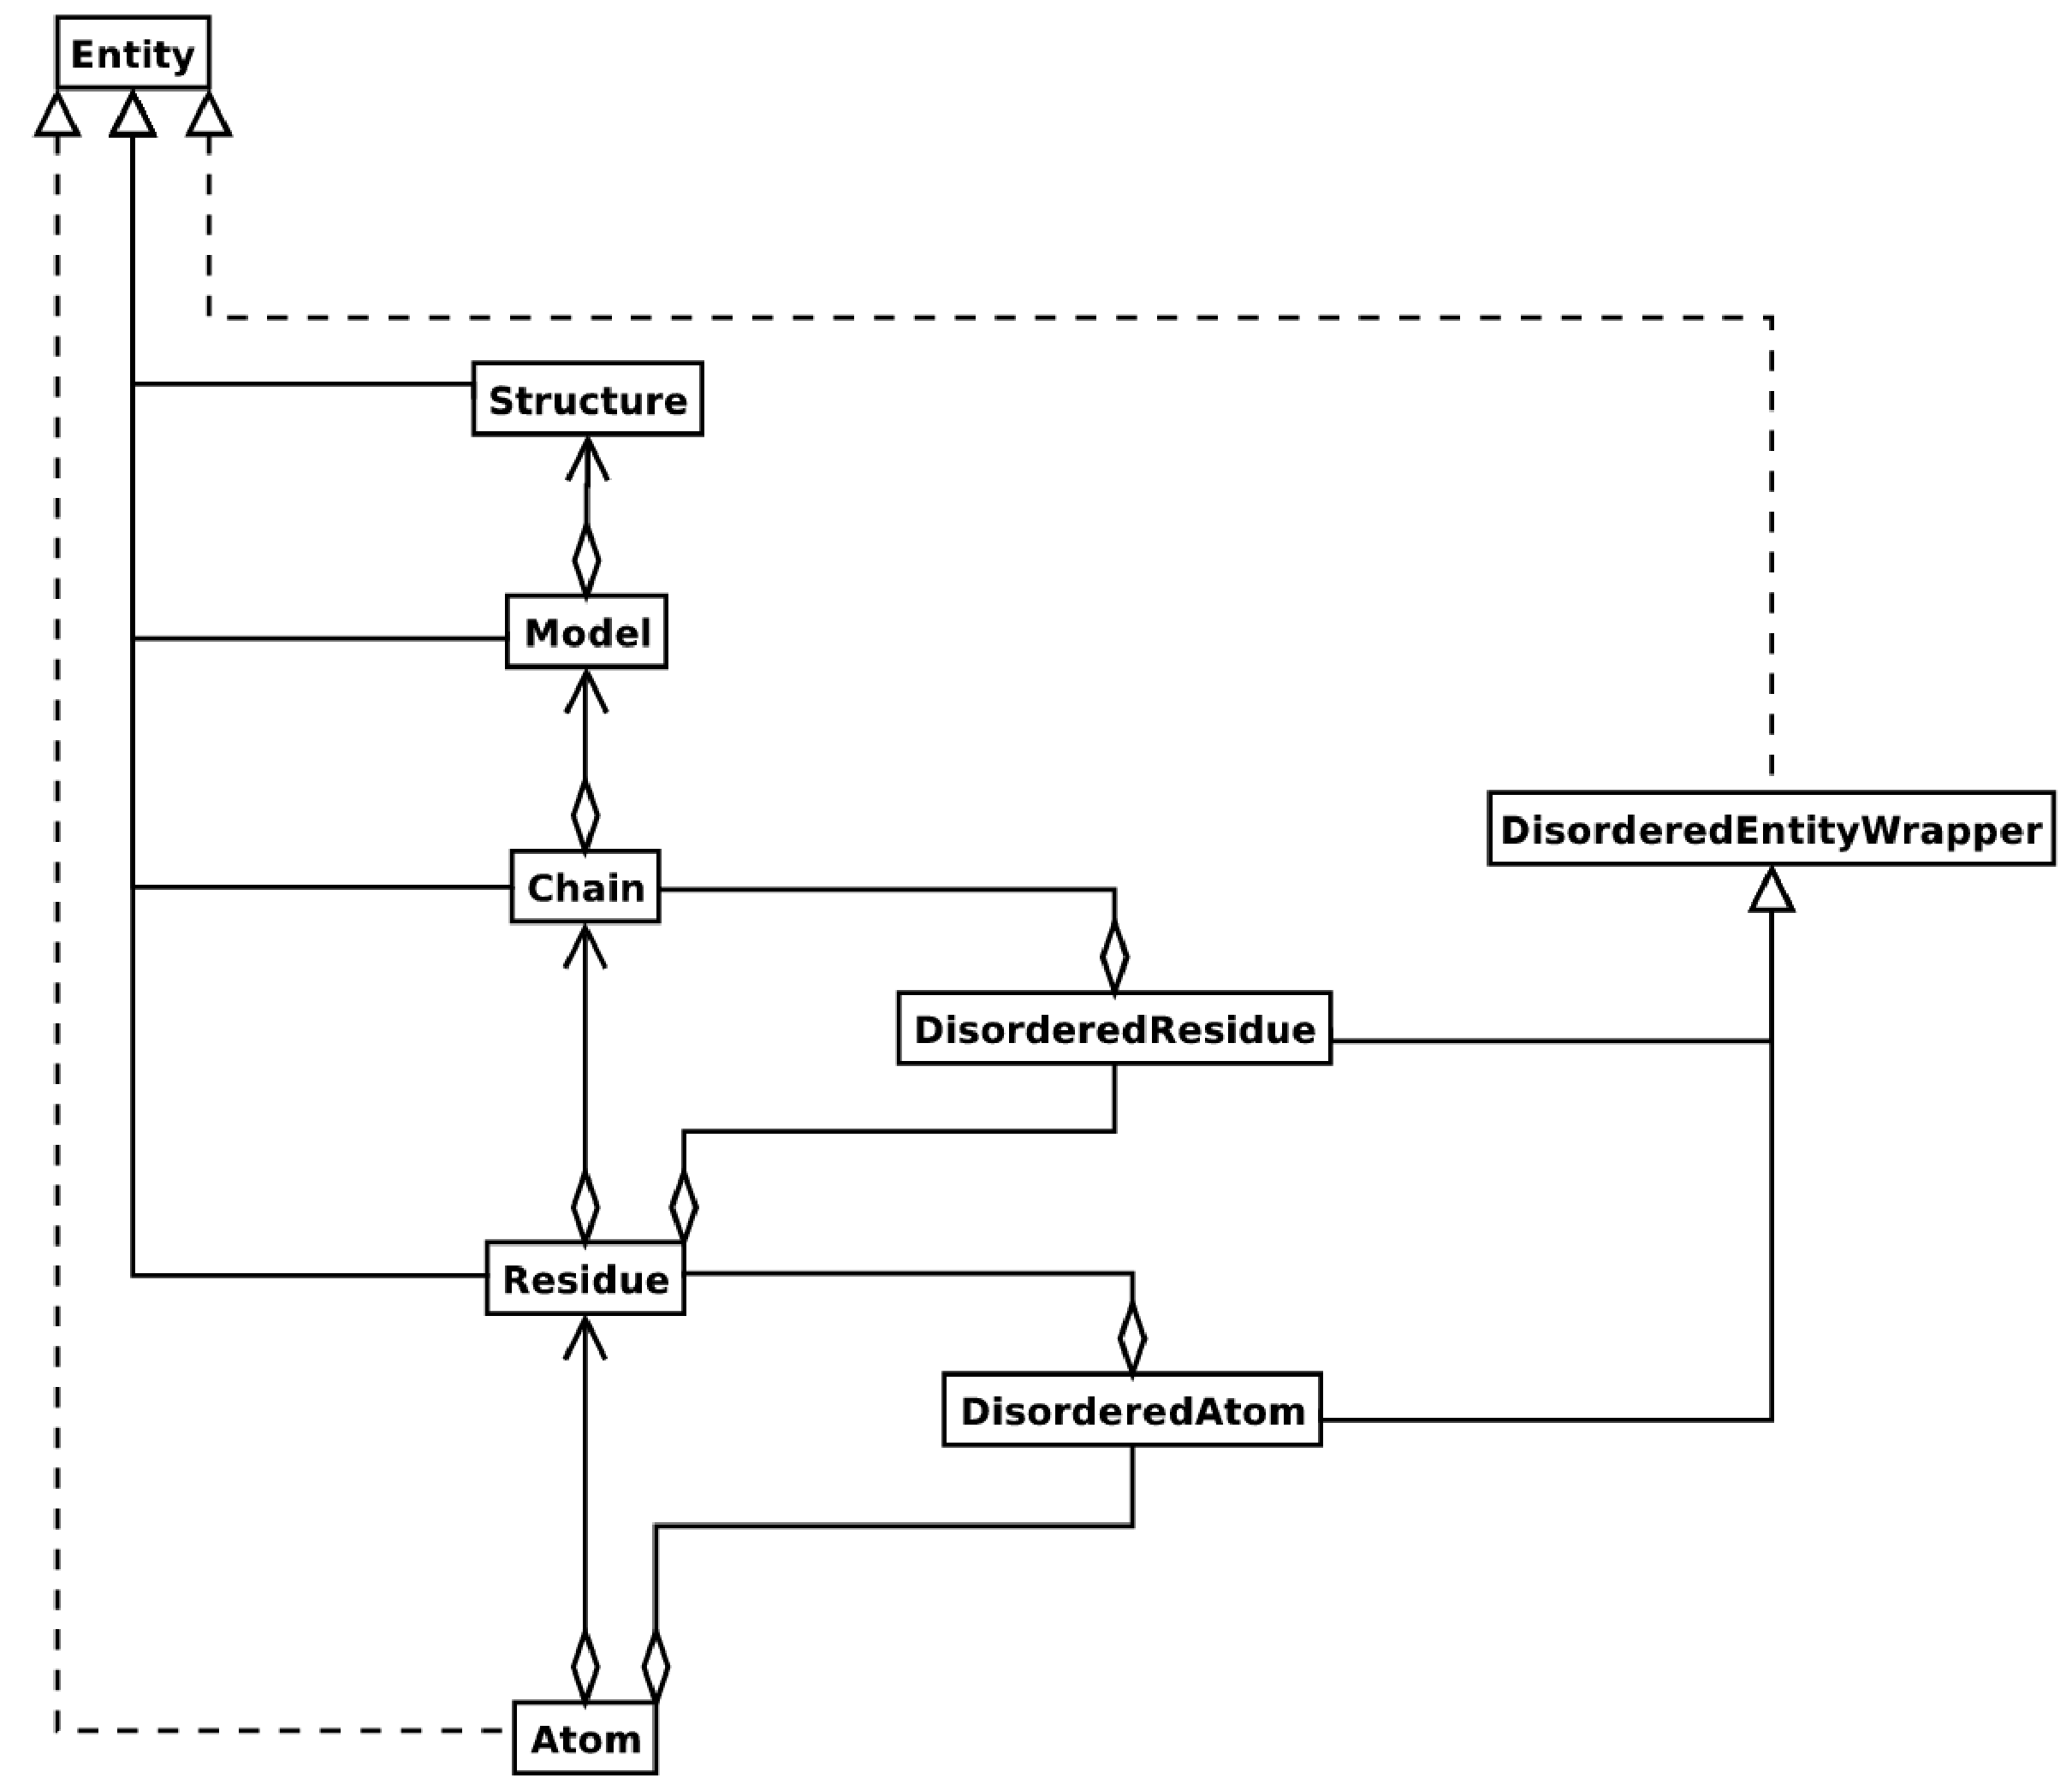
\includegraphics[width=0.8\textwidth]{images/smcra.eps}
\label{fig:smcra}
\caption{��ʬ�ҹ�¤��ɽ������ݤ˻Ȥ��� SMCRA �ǡ�����¤�� UML ���饹��}
\end{figure}

\class{Structure}��\class{Model}��\class{Chain} ����� \class{Residue}
�ϡ����������쥯�饹 \class{Entity} (����ƥ��ƥ�) �Υ��֥��饹�Ǥ���
\class{Atom} ���饹������\class{Entity} ���󥿡��ե������ΰ�������
�������Ƥ��ޤ��� (\class{Atom} ���饹�ˤϻҥ��饹��ɬ�פʤ�����Ǥ�)��

\class{Entity} ���֥��饹�Υ��֥������Ȥϡ���������դʼ��̻�
(id) �򥭡��˻Ȥ����Ȥǡ���ʬ�λҥ���ƥ��ƥ�����Ф��ޤ� (�㤨�С�
���Ҥ�̾����ɽ��ʸ����򥭡��ˤ��ơ����� \class{Residue} ���֥�������
����\class{Atom} ���֥������Ȥ���Ф����ꡤʬ�Һ��� id �򥭡���
���ơ�\class{Model} ���֥������Ȥ��� \class{Chain} ���֥������Ȥ�
���Ф�����Ǥ��ޤ�)��

���Ҥ�Ĵ�Τ�餮 (disorder) �� \class{DisorderedAtom} ��
\class{DisorderedResidue} ���饹��ɽ������ޤ��������Ϥ������
���쥯�饹\class{DisorderedEntityWrapper} �Υ��֥��饹�Ǥ���
�����Υ��饹�ϡ���餮��ȼ��ʣ�������ä��������������̤�
\class{Atom} �� \class{Residue} ���֥������ȤǤ��뤫�Τ褦�˿�����
�ޤ���

����Ū�ˤϡ�����ƥ���ƥ��ƥ� (\class{Residue}, \class{Chain},
\class{Model}, \class{Structure}) �λҤˤ����륨��ƥ��ƥ����֥�������
(\class{Atom}, \class{Residue}, \class{Model}, \class{Structure}) �ϡ�
id �򥭡��ˤ��Ƽ��Ф��ޤ���

\begin{verbatim}
child_entity=parent_entity[child_id]
\end{verbatim}

�ޤ�������ƥ���ƥ��ƥ����֥������Ȥλҥ���ƥ��ƥ����ƤΥꥹ�Ȥ�
���Ф��ޤ������Υꥹ�Ȥ��ü�ʤ�꤫�����¤�Ǥ���Τ����դ��Ƥ�����
�� (�㤨�С�\class{Model} ���֥������Ȥ��Ƥξ�硤�Ҥ�\class{Chain} 
���֥������Ȥ�¦�� id (chain identifier) �˱������¤Ӥޤ�)��

\begin{verbatim}
child_list=parent_entity.get_list()
\end{verbatim}

����ҥ���ƥ��ƥ����֥������Ȥοƥ���ƥ��ƥ����֥������Ȥ�
���Ф��ޤ���

\begin{verbatim}
parent_entity=child_entity.get_parent()
\end{verbatim}

�ޤ���SMCRA ���ؤΤɤγ��ؤΥ��֥������Ȥ��Ф��Ƥ⡤
\emph{���� id (full id)} ����Ф��ޤ���
���� id �Ȥϡ��Ǿ�̤Υ��֥������� (\class{Structure}) ���鲼�äơ�
���ߤΥ��֥������Ȥޤ�é�ä��Ȥ��˷�ͳ�������ƤΥ��֥������Ȥ� id ����
�ʤ륿�ץ�Ǥ����㤨�С����� \class{Residue} ���֥������Ȥδ��� id ��
�ʲ��Τ褦�ˤʤ�ޤ�:

\begin{verbatim}
full_id=residue.get_full_id()

print full_id

("1abc", 0, "A", ("", 10, "A"))
\end{verbatim}

���Υ��ץ�����Ƥϡ����줾��

\begin{itemize}
\item \code{"1abc"} �� id �˻��� \class{Structure} ���֥�������
\item \code{0} �� id �˻��� \class{Model} ���֥�������
\item \code{"A"} �� id �˻��� \class{Chain} ���֥�������
\item \code{("", 10, "A")} �� id �˻��� \class{Residue} ���֥�������
\end{itemize}

���б����ޤ���

�Ǹ�� \class{Residue} ���֥������Ȥ� id �ϡ��إƥ��ե������
(�ǽ�Υե������) ������ˤʤäƤ��ޤ�������ϡ����λĴ�
�إƥ��Ĵ� (�⤷���Ͽ�) �ǤϤʤ����Ȥ򼨤��Ƥ��ޤ����ޤ���
����μ��̻Ҥ� 10 �ǡ����������� (insertion code) �� \code{"A"} 
�ˤʤäƤ��ޤ���

����ƥ��ƥ��ˤϤ����Ĥ������ʥ᥽�åɤ�����ޤ�:

\begin{verbatim}
# ����ƥ��ƥ��� id ������

entity.get_id()

# ���� id ���ä��ҥ���ƥ��ƥ���¸�ߤ��뤫��Ĵ�٤�

entity.has_id(entity_id)

# �ҥ���ƥ��ƥ��ο�������

nr_children=len(entity)
\end{verbatim}

����ƥ���ƥ��ƥ����Ф��ơ����λҥ���ƥ��ƥ����������ꡤ
�ҥ���ƥ��ƥ���̾�����ѹ������ꡤ�����ʻҥ���ƥ��ƥ����ɲä������
�Ǥ��ޤ��������κݤ˥ǡ����������������å� (sanity check) ��
�Ԥ��ޤ��� (�㤨�С�����ʬ�Һ���Ʊ�� id �������ĤλĴ��
�ղä�����Ǥ��Ƥ��ޤ��ޤ�)��\class{Decorator} ���饹���Ѥ���ȡ�
��������ޤ᤿�������������å��򤦤ޤ��ԤäƤ���ޤ������⤷
�ǤΥ��󥿥ե����������Ѥ������ʤ顤������������ (\file{Entity.py})
�򻲾Ȥ��ƤߤƤ���������

\subsubsection{Structure ���֥�������}

\class{Structure} ���֥������ȤϹ�ʬ�Ҥ�ɽ������ǡ����γ��ع�¤��
ĺ���˰��֤��Ƥ��ޤ���\class{Structure} �� id �ϥ桼�������ꤷ��
ʸ����ˤʤ�ޤ���\class{Structure} ���֥������Ȥˤϡ�ʣ����
\class{Model} ���֥������Ȥ��ҥ���ƥ��ƥ��Ȥ������äƤ��ޤ���
�ۤȤ�ɤ� (���ƤǤϤ���ޤ���) �뾽��¤�ˤ�ñ��Υ�ǥ뤷��
�ʤ������� NMR �Ƿ��ꤵ��빽¤�ˤϰ���Ū�ˤ����Ĥ��Υ�ǥ뤬
���äƤ��ޤ����뾽��¤�ˤ�����¿����ʬ�Ҥˤ�餮�������Ƥ�����
�ˤ⡤ʣ���Υ�ǥ뤬�Ǥ��ޤ���

\paragraph{Structure ���֥������Ȥ��ۤ���}

\class{Structure} ���֥������Ȥ� \class{PDBParser} ���֥������Ȥ���
��������ޤ�:

\begin{verbatim}
from Bio.PDB.PDBParser import PDBParser

p=PDBParser(PERMISSIVE=1)

structure_id="1fat"

filename="pdb1fat.ent"

s=p.get_structure(structure_id, filename)
\end{verbatim}

\var{PERMISSIVE} �ե饰�ϡ�PDB �ե�����˴ؤ���褯���뤤���Ĥ�������
(\ref{problem structures} ����) ��ѡ�����̵�뤵���ޤ� (�ȤϤ�����
����ˤ�äƤ����Ĥ��θ��Ҥ�Ĵ𤬼����뤫�⤷��ʤ��Τ����դ���
��������) �����Τ��Υե饰����ꤷ�ʤ���硤�ѡ����� PDB �ե������
��ʸ���Ϥ��Ƥ���ݤ����꤬�������\exception{PDBConstructionException}
�����Ф��ޤ���

\paragraph{�إå� (header) �ȥȥ쥤�� (trailer)}

\function{get_header} ����� \function{get_trailer} �Ȥ��ä��᥽�åɤ�
�Ѥ���ȡ�PDB �ե�������Υإå��ȥȥ쥤��� (ʸ���󤫤�ʤ�ñ��ʥꥹ��
��) \class{PDBParser} ���֥������Ȥ�����Ф��ޤ���

\subsubsection{Model ���֥�������}

\class{Model} ���֥������Ȥ� id �������ǡ�PDB �ե��������Ϥ����ݤ�
���Υ�ǥ뤬���֤��Ƥ�����꤫���ޤ�ޤ� (0 ���鼫ưŪ���ֹ��դ�
����ޤ�)��\class{Model} ���֥������Ȥˤϡ��ҥ���ƥ��ƥ���\class{Chain} 
����ʤ�ꥹ�Ȥ����äƤ��ޤ���


\paragraph{����}

\class{Structure} ���֥���������˼�����Ƥ���ǽ��
��ǥ��������ޤ���

\begin{verbatim}
first_model=structure[0]
\end{verbatim}

\subsubsection{Chain ���֥�������}

\class{Chain} ���֥������Ȥ� id �ϡ���¤�ǡ������ҥե��������
��������ʬ�Һ���ɽ����ʬ�μ��̻Ҥ���Ȥ�졤���餫��ʸ����ˤʤ�ޤ���
����\class{Model} ���֥������Ȳ��ˤ���ơ���\class{Chain} �ˤ�
�ߤ��˰�դ� id ������ޤ���\class{Chain} ���֥������Ȥˤ�
�ҥ���ƥ��ƥ���\class{Residue} ����ʤ�ꥹ�Ȥ����äƤ��ޤ���

\paragraph{����}

\class{Model} ���֥������Ȥ��顤���̻� \code{"A"} ���ä�
\class{Chain} ���֥������Ȥ�������ޤ���

\begin{verbatim}
chain_A=model["A"]
\end{verbatim}

\subsubsection{Residue ���֥�������}

�����ޤǤ�ʤ���\class{Residue} �ϰ�Ϣ��\class{Atom} ��ҥ���ƥ��ƥ�
�Ȥ��Ƶ������Ƥ��ޤ�������˲ä��ơ�\class{Residue} �ˤϻĴ��̾��
�򼨤�ʸ���� (�㤨�� \code{"ASN"}) �ȡ��Ĵ�Υ������ȼ��̻�
(X-PLOR �桼���ˤϤ褯�Τ��Ƥ��ޤ�����SMCRA �ǡ�����¤���ۤ���
�ݤˤ��Ѥ����ޤ���) �����äƤ��ޤ���

\class{Residue} ���֥������Ȥ� id �ϻ��Ĥ���ʬ: �إƥ��ե������
(hetfield)�������̻� (resseq)������������ (icode) ����ʤ�ޤ���

�إƥ��ե�����ɤ�ʸ����ǡ�\code{"W"} �Ͽ��\code{"H_"} �θ����
�Ĵ�̾��³������� (�㤨�� \code{"H_FUC"}) �Ϥ���¾�Υإƥ��Ĵ��
����ϰ���Ū�ʥ��ߥλ��ȳ˻���ɽ���ޤ���������ˡ����Ѥ�����ͳ��
\ref{hetero problems} ��Dz��⤷�Ƥ��ޤ���

�Ĵ� id ������Υե�����ɤ������̻Ҥǡ�ʬ�Һ���
�ɤξ��˻Ĵ𤬷�礷�Ƥ��뤫��ɽ���ޤ���

�軰�Υե�����ɤ�ʸ����ǡ����������ɤ�����ޤ������������ɤ�
���Ф��С�����λĴ���Ф���˾�ޤ������ֹ��դ���ˡ����¸���뤿���
�Ȥ��ޤ���Ser 80 �����ߥ塼����� (�㤨�С�Thr 80 �� Asn81 �Ĵ��
�֤� Ser �����ä����) �ξ�硤�����̻Ҥ����������ɤϤ��줾��
Thr 80 A, Ser 80 B, Asn 81 �Τ褦�ˤʤ�ޤ���������ˡ��Ȥ�ȡ�
�Ĵ���ֹ��դ���ˡ���������ι�����Ʊ���ޤޤˤʤ�ޤ���

�����Ĥ����󤲤Ƥߤޤ��礦�� ���������ɤ�����ˤʤäƤ��� Asn 10 
�λĴ� id ��\code{("", 10, "")} �Ǥ���W 10 �λĴ� id ��
\code{("W", 10, "")} �Ǥ��������̻� 10 �Υ��륳����ʬ�� (�إƥ�
�Ĵ� GLC �Ȥ���̾���ˤʤäƤ��ޤ�) �� \code{("H_GLC", 10, "")}
�Ǥ������Τ褦�ˤ���ȡ����ƤλĴ�ϰۤʤ�Ĵ� id ����ĤΤǡ�
Ʊ��ʬ�Һ��ΰ���ʬ�Ȥ��ư����ޤ���

�ۤȤ�ɤξ�硤 \member{hetflag} �� \member{icode} �ե�����ɤ϶���
���ʤ��\code{("W", 10, "")} �Τ褦�ˤʤ�ޤ������Τ褦�ʾ��ˤϡ�
�����̻Ҥϴ��� id �Υ��硼�ȥ��åȤȤ������ѤǤ��ޤ�:

\begin{verbatim}
# ���� id ���

res10=chain[("", 10, "")]

# ���硼�ȥ��åȤλ��� 

res10=chain[10]
\end{verbatim}

\class{Chain} ���֥������Ⱦ�γ� \class{Residue} ���֥������Ȥˤ�
��դ� id ���Ĥ����Ƥ��ޤ����Ĵ�Τ�餮�����̰�������ޤ���
����ˤĤ��Ƥ�\ref{point mutations} ����������ޤ���

\class{Residue} ���֥������Ȥˤϡ�¾�ˤ⤤���Ĥ��᥽�åɤ�����ޤ�:

\begin{verbatim}
r.get_resname()         # "ASN" �Τ褦�ʻĴ�̾���֤�
r.get_segid()           # "CHN1" �Τ褦�� SEGID ���֤�
\end{verbatim}

\subsubsection{Atom}

\class{Atom} �ϸ��Ҥ˴�Ϣ����ǡ����򵭲������ҥ���ƥ��ƥ�������ޤ���
���Ҥ� id �Ϥ��θ��Ҥ�̾���ˤʤ�ޤ� (�㤨�С�\code{"OG"} �� Ser �Ĵ��
¦���λ��ǤǤ�)������Ĵ���Ǥϡ��ġ��θ��Ҥ� id �ϰ�դǤʤ����
�ʤ�ޤ���\ref{disordered atoms} ��Ǥ�Ҥ٤��褦�ˡ��ǡ�����ʸ����
����ݤ˸��ҤΤ�餮������������㳰��ȯ�����ޤ���

PDB �ե�������Ǥϡ����Ҥ�̾���� 4 ʸ���Υ���饯������ʤꡤ�̾��
��Ƭ�������˶��򤬤Ĥ��Ƥ��ޤ���PDB �ե�����Ǥϡ���ñ�Τ����
���Ф��Ф��ζ���Ͻ����ޤ� (�㤨�С����ߥλ�C$\alpha$ ��
PDB �ե�������Ǥ� \code{".CA."} �ǡ��ɥåȤ������ɽ���ޤ�)��
����Ĵ����̾���ξ��� (Ʊ��̾���� id ����� \class{Atom} ���֥�������
�����������) ��������ʤ��¤ꡤ���Ҥ�̾������������ݤ˥��ڡ�����
����ޤ������ͤ�ȯ�������硤�ѡ����ϥ��ڡ�����ޤ᤿����̾��Ȥ�����
��ߤޤ������Τ褦�ʾ����ϡ��㤨�а�ĤλĴ�� \code{".CA."} ��
\code{"CA.."} �Ȥ���̾���θ��Ҥ����äƤ������ȯ�����ޤ�����
��ä��˵����뤳�ȤϤ���ޤ���

�Ĵ����¸����Ƥ��븶�ҤΥǡ����ˤϡ����Ҥ�̾�������Ҥκ�ɸ
(�⤷�����ɸ���к���)��B �ե����� (�⤷����а����� B �ե�������
ɸ���к���)�� altloc ����Ҥȶ����ޤര���ʸ���̾�����äƤ��ޤ���
�����ֹ� (element number) �丶�Ҥ��Ų٤Ȥ��ä������ޤ����Ѥ���ʤ�
���Ǥϡ� PDB �ե�������ˤϽ񤫤�Ƥ��ޤ���\class{Atom} �Υǡ�����
���Ƥ���¸����ޤ���

\class{Atom} ���֥������Ȥˤϰʲ��Τ褦�ʥ᥽�åɤ�����ޤ�: 

\begin{verbatim}
a.get_name()       # ����̾ (���ڡ����ʤ����㤨�� "CA")

a.get_id()         # id (����̾��Ʊ��)

a.get_coord()      # ���Һ�ɸ

a.get_bfactor()    # B �ե�����

a.get_occupancy()  # ���Ҥ�餮�ˤ�������ͭΨ

a.get_altloc()     # _REPLACE_���ع�¤�������ֻ���� (alternative location specifier) 

a.get_sigatm()     # ���ҥѥ�᥿��ɸ���к�

a.get_siguij()     # ������ B �ե�������ɸ���к�

a.get_anisou()     # ������ B �ե�����

a.get_fullname()   # ����̾ (���ڡ�����ޤ�, ��. ".CA.")
\end{verbatim}

���Ҥκ�ɸ�������� B �ե���������Ӥ���ɸ���к���
���ҥѥ�᥿��ɸ���к���ɽ���ˤ� Numerical Python ������
�Ѥ����Ƥ��ޤ���

\subsection{��餮 (disorder)}


\subsubsection{����Ū�ʥ��ץ�����}
\label{disorder problems}

ʬ�ҹ�¤�Τ�餮 (disorder) ��ͤ���ˤϡ���Ĥλ���������ޤ���
��Ĥϸ��ҤΤ�餮���⤦��ĤϻĴ�Τ�餮�Ǥ��������Ƥ����桹��
��餮���餯��ʣ���������ƥ��ץ��벽���ư������Ȥ��Ƥ��ޤ��ޤ���
���������⤷����ñ�����Ƥ� C$\alpha$ ���Ҥˤ錄�äƥ롼�׽�����
�Ԥ����������ʤ顤�ɤ����λĴ��¦���ˤ�餮�����äƤⵤ�ˤ�
���ޤ��󡥤��ΰ����ǡ��ǡ�����¤��Ǥϡ���餮������ɽ��
�Ǥ��ʤ���Фʤ�ʤ��Ȥ������꤬����ޤ��������ǡ����Ҥ�Ĵ��
��餮���ü�ʥ��֥������Ȥ����졤���������餮��¸�ߤ��ʤ�����
�褦�˿���碌�뤳�Ȥˤ��ޤ�����������������Ԥ�ͣ�����ˡ�ϡ�
��餮����ĸ��Ҥ�Ĵ�Υ��֥��åȤˤ��ɽ���Ǥ����ɤΥ��֥��åȤ�
���Ѥ��뤫 (�㤨�С�Ser �Ĵ𤬻Ȥ��Ƥ�����ǡ����̤�ˤ�餮��
���� OG ¦���Τɤ�������֤�) �ϡ��桼��������Ǥ��ޤ���


\subsubsection{���ҤΤ�餮}
\label{disordered atoms}

���ҤΤ�餮�ξ�硤��餮�Τ�����ʬ�θ��Ҥ��̾��\class{Atom} 
���֥������Ȥ�Ȥä�ɽ�����ޤ��������������θ��Ҥ�ʪ��Ū��Ʊ��
���Ҥ�ɽ�����Ƥ���褦�ʸ��Ҥϡ����� \class{DisorderedAtom} 
���֥������������¸���ޤ���\class{DisorderedAtom} ���֥����������
��\class{Atom} ���֥������Ȥϡ�\member{altloc} ����Ҥ�Ȥäư�դ�
����Ǥ��ޤ���
\class{DisorderedAtom} ���Ф��ƥ᥽�åɸƤӽФ���Ԥ��ȡ�
\class{DisorderedAtom} �ǽ�������ʤ���Τϸ������򤵤�Ƥ���
\class{Atom} ���֥������Ȥ�ž�����ޤ����ǥե���ȤǤϡ�
��ͭΨ (occupancy) �κǤ�⤤\class{Atom} ���֥������Ȥ����򤵤��
���ޤ����������\member{altloc} �����Ѥ���С��桼���Ϥ����줫��
\class{Atom} ���֥������Ȥ�����Ǥ��ޤ������Τ褦�ˤ��ơ�������ʣ����
���������Ȥʤ������Ҥ�餮��������ɽ���Ǥ���褦�ˤʤäƤ���ΤǤ���
�̤θ������򤹤�С����Ҥ�餮�˶�̣���ʤ���С�����ˤ鷺��蘆���
ɬ�פϤʤ��Ȥ������ȤǤ���

��餮�θ��Ҥˤϡ����줾�� \member{altloc} �Ȥ������̻Ҥ�����ޤ���
\class{DisorderedAtom} ���֥������Ȥˤ��μ��̻Ҥ���ꤹ��ȡ�
����� \member{altloc} ���̻Ҥ���ä� \class{Atom} �Ǥ��뤫�Τ褦��
����碌���ޤ�:

\begin{verbatim}
atom.disordered_select("A")        # altloc �� A �θ��Ҥ����򤹤�
print atom.get_altloc()
"A"

atom.disordered_select("B")        # altloc �� B �θ��Ҥ����򤹤�
print atom.get_altloc()
"B"
\end{verbatim}

\subsubsection{�Ĵ�Τ�餮}

\paragraph{�褯���륱����}

��äȤ�褯����Τϡ��Ĵ�˰�Ĥޤ��Ϥ���ʾ�θ��ҤΤ�餮��
���륱�����Ǥ��������ޤǤ�ʤ������Υ�������\class{DisorderedAtom} 
���֥������Ȥˤ�äƤ�餮�Τ��븶�Ҥ�ɽ����������
\class{DisorderedAtom} ���֥������Ȥ�\class{Residue} ���֥������Ȥ�
������̤�\class{Atom} ���֥������ȤΤ褦�ˤ��������в�褷�ޤ���
\class{DisorderedAtom} �ϡ���ʬ��Ŭ�Ѥ��줿�᥽�åɤΤ�����
\class{DisorderedAtom} �ǽ�������ʤ���Τ�������\class{Atom} 
���֥������� (���򤵤�Ƥ��� \class{Atom} ���֥�������) 
��ž�����뤳�Ȥǡ����������̾�θ��ҤȤޤä���Ʊ���褦�� 
(�ºݤˤϺǤ���ͭΨ�ι⤤���Ҥ�Ʊ���褦��) �����񤤤ޤ���

\paragraph{���Ѱ�}
\label{point mutations}
��餮�����Ѱ� (point mutation) ��ͳ�褹��褦���ü�ʥ�������
�㤨�����Ѱ��Τ���İʾ庮���ä��ݥ�ڥץ��ɤ��뾽��˸��Ĥ���褦��
��礬����ޤ������Τ褦����ΰ�Ĥ� PDB ��¤�� 1EN2 �Ǥ���

���������ѰۤǤϡ��Ĵ� (�㤨�� Ser 60 �� Cys 60 �Τ褦��) �ۤʤ�
�Ĵ𷿤�°����Τǡ���Τ褯������Τ褦�ˡ���Ĥ� \class{Residue}
���֥������Ȥ���ˤ�����ޤ��󡥤��Τ褦�ʥ������Ǥϡ�
��餮�Ȥʤ�ơ��λĴ��\class{Residue} ���֥������Ȥ�ɽ�����Ƥ�����
ξ���� \class{Residue} ���֥������Ȥ� \class{DisorderedResidue}
���֥������Ȥ�����Ƥ����ޤ��� 

\class{DisorderedResidue} �ϡ���ʬ��Ŭ�Ѥ��줿�᥽�åɤΤ�����
\class{DisorderedResidue} �ǽ�������ʤ���Τ򸽺����򤵤��
����\class{Residue} ���֥������� (�ǥե���ȤǤϺǸ���ɲ�
���줿\class{Residue} ���֥�������) ��ž�����뤳�Ȥǡ�
���������̾�λĴ�Τ褦�˿��񤤤ޤ���\class{DisorderedResidue} 
���֥���������γ�\class{Residue} ���֥������Ȥϡ��ơ���
�Ĵ�̾�ǰ�դ˼��̤Ǥ��ޤ��������Ǥ����С� 
\class{DisorderedResidue} ���֥���������� Ser 60 �Ĵ��
���̻Ҥ�\code{"SER"} ��Cys 60 �μ��̻Ҥ�\code{"CYS"} �Ǥ���
�桼���Ϥ��μ��� id ��ȤäƸ���ͭ���� \class{Residue} ���֥�������
������Ǥ��ޤ���

\subsection{�إƥ��Ĵ�}

\subsubsection{�إƥ��Ĵ�˴�Ϣ��������}
\label{hetero problems}

�إƥ��Ĵ�˴ؤ��Ƥ褯��������ϡ������Ĥ��Υإƥ��Ĵ����إƥ��Ĵ��Ʊ��
����������Ʊ��������̻�(����������������)��ͭ���뤳�ȤǤ��롣��
�Τ��ᡢ�Ƥإƥ��Ĵ���ȼ���id���������뤿���Ȥ���¾�Υإƥ��Ĵ�ϰ�
�ʤ���ˡ�ǰ����롣

�إƥ��Ĵ�˴ؤ��Ƥ褯��������ϡ�Ʊ��ʬ�Һ���ˤ���ʣ���Υإƥ��Ĵ�
��إƥ��Ĵ𤬡�Ʊ�������̻�(���������������) ����äƤ����
�������ȤǤ����������äơ��ƥإƥ��Ĵ�� id ���դ��������뤿��ˡ�
��䤽��¾�Υإƥ��Ĵ���̤���ˡ�ǰ����ޤ���

\class{Residue} ���֥������Ȥ� \code{(hetfield, resseq, icode)} �Ȥ���
���ץ�� id ����äƤ��뤳�Ȥ�פ��Ф��Ƥ������������ߥλ���˻���
��硤 \member{hetfield} �϶� (\code{""}) �ˤʤꡤ���إƥ��Ĵ�ξ��ˤ�
ʸ����ˤʤ�ޤ���\member{hetfield} �����ƤˤĤ��Ƥϡ��ʲ����������ޤ���

\subsubsection{��Ĵ�}

��Ĵ�� \member{hetfield} ��ʸ����� \code{"W"} �ˤʤ�ޤ������Τ��ᡤ
��ΰ���Ū��id�� \code{("W", 1, "")} �Ǥ���

\subsubsection{����¾�Υإƥ��Ĵ�}

����¾�Υإƥ��Ĵ�� \member{hetfield} ʸ����ϡ�\code{"H_"} �˻Ĵ�̾��
³������ΤǤ����㤨�С��Ĵ�̾ \code{"GLC"} �Υ��륳����ʬ�Ҥξ�硤
\member{hetfield} �� \code{"H_GLC"} �ˤʤ�ޤ����Ĵ� id �� 
\code{("H_GLC", 1, "")} �Ǥ���

\subsection{������}

PDB�ե��������Ϥ��ơ�\class{Model}��\class{Chain}�� \class{Residue}
����ӡ�\class{Atom} ���֥������Ȥ���Ф��ޤ���

\begin{verbatim}
from PDBParser import PDBParser 

parser=PDBParser()

structure=parser.get_structure("test", "1fat.pdb")
model=structure[0]
chain=model["A"]
residue=chain[1]
atom=residue["CA"]
\end{verbatim}

ʬ�Һ�����إƥ��Ĵ� (�����Ǥϰ����� resseq 10 �Υ��륳���� (GLC) 
�Ǥ���褦�ʻĴ�) ����Ф��ޤ���

\begin{verbatim}
residue_id=("H_GLC", 10, " ")
residue=chain[residue_id]
\end{verbatim}

ʬ�Һ�������ƤΥإƥ��Ĵ����Ϥ��ޤ���

\begin{verbatim}
for residue in chain.get_list():
	residue_id=residue.get_id()
	hetfield=residue_id[0]
	if hetfield[0]=="H":
		print residue_id
\end{verbatim}

B �ե������� 50 �ʾ�� CA ���Ҥκ�ɸ�����ƽ��Ϥ��ޤ���

\begin{verbatim}
for model in structure.get_list():
  for chain in model.get_list():
    for residue in chain.get_list():
      if residue.has_id("CA"):
        ca=residue["CA"]
        if ca.get_bfactor()>50.0:
          print ca.get_coord()
\end{verbatim}

��餮�Τ��븶�Ҥ�ޤ����ƤλĴ����Ϥ��ޤ���

\begin{verbatim}
for model in structure.get_list()
  for chain in model.get_list():
    for residue in chain.get_list():
      if residue.is_disordered():
        resseq=residue.get_id()[1]
        resname=residue.get_resname()
        model_id=model.get_id()
        chain_id=chain.get_id()
        print model_id, chain_id, resname, resseq
\end{verbatim}

��餮�Τ��븶�����Ƥˤ錄�äƥ롼�פ��ơ����� \member{altloc} �� 
\code{"A"} �θ��� (�������) �ˤʤ�褦���򤷤ޤ�����������Ԥ��ȡ�
SMCRA �ǡ�����¤�ε�ư�� \member{altloc} �� \code{"A"} �θ��Ҥ���
¸�ߤ��ʤ����ε�ư�ˤ��ޤ���

\begin{verbatim}
for model in structure.get_list()
  for chain in model.get_list():
    for residue in chain.get_list():
      if residue.is_disordered():
        for atom in residue.get_list():
          if atom.is_disordered():
            if atom.disordered_has_id("A"):
              atom.disordered_select("A")
\end{verbatim}

ʬ�Һ��ΰ��� 10 �����Ѱۤ����äơ� Ser �� Cys ����ʤ�Ȥ��ޤ���
ʬ�Һ��ε�ư����� 10 �λĴ� Cys �Ĵ�Ǥ�����ε�ư�ˤ��ޤ���

\begin{verbatim}
residue=chain[10]
residue.disordered_select("CYS")
\end{verbatim}

\subsection{PDB �ե�����ˤ褯��������}
\subsubsection{��}
\label{problem structures}
\class{PDBParser}/\class{Structure} ���饹�ϡ�
(�ơ� SCOP �ǰۤʤ� �����ѡ��ե��ߥ꡼��°���Ƥ���) �� 800 ��
����ѥ���¤�ǥƥ��Ȥ�Ԥ��ޤ����������ˤ��� 20 ʬ���פ���
�칽¤�������ʿ�Ѥ� 1.5 �äǤ����� 64000 ���Ҥ�ޤ��ܥ������
�祵�֥�˥å� (1FKK) �Υǡ�����¤���Ϥˤϡ� 1000 MHz �� PC ���
10 �ä�����ޤ�����

���Υƥ��Ȥ���ǡ������ޤ��Ǥʤ��ǡ�����¤���ۤǤ��ʤ��Ȥ�����ͳ��
�㳰�� 3 �����Ф���ޤ�����������Υ������ˤ����Ƥ⡤���顼�θ�����
PDB �ե�����¦�ǽ������٤�����Ǥ��������������������Ǥϡ��㳰��
���Ф����������ǡ�����¤�˽񤫤�Ƥ������Ƥ���ä�ɽ�����Ƥ��ޤ�
����Ϥ뤫�ˤޤ��Ǥ���

\paragraph{�Ĵ�ν�ʣ (duplicate residues)}

���빽¤�Ǥϡ���Ĥ�ʬ�Һ������ĤΥ��ߥλ��Ĵ�Ʊ�������̻�
(resseq 3) �� icode ����äƤ��ޤ�����Ĵ�٤��Ȥ�����
����ʬ�Һ��� Thr A3, \ldots{}, Gly A202, Leu A3, Glu A204 �Τ褦��
�ʤäƤ��ޤ�����Leu A3 ���������� A203 �ʤΤ����餫�Ǥ���
Ʊ���褦�ʾ����� 1FFK �ˤ⤢��ޤ��� (Gly B64, Met B65, Glu B65, 
Thr B67, �ĤޤꡤGlu B65 �� Glu B66 �θ���)��


\paragraph{���Ҥν�ʣ (duplicate atoms)}

ʬ�ҹ�¤ 1EJG �ϡ�ʬ�Һ� A �� 22 ���ܤλĴ� Ser/Pro �����Ѱۤ�
�ʤäƤ��ޤ�������ˡ� Ser 22 �Τ����Ĥ��θ��ҤϤ�餮����äƤ��ޤ���
�������̤ꡤSer22 ��°�������Ƥθ��Ҥˤ϶���Ǥʤ� \member{altloc}
����� (B �ޤ��� C) �����ꡤPro 22 �����Ƥθ��Ҥ� \member{altloc} A
�Ǥ��������������� N �� \member{altloc} ����������ˤʤäƤ��ޤ�����
���줬�㳰�����Ф��븶���ˤʤäƤ��ޤ������Ȥ����Τ⡤���Ѱۤ�
�����Ƥ�����Ǥϡ������λĴ�������äƤ������Ƥθ��Ҥ˶���Ǥʤ�
\member{altloc} ���Ĥ��Ƥ��ʤ���Фʤ�ʤ�����Ǥ���Ser 22 �ˤ�
���� N ���ʤ��ä��Τǡ������餯���θ��Ҥ� Ser 22 �� Pro 22 �δ֤�
��ͭ����Ƥ���Τ������Ȥ������Ȥ�狼��ޤ��������ޤ���
�ե�����ˤ�����������󵯤��Ƥ��ޤ�: ���� N �� Ser �� Pro �Ĵ��
ξ���ˤʤ��ƤϤʤ餺������Ŭ�ڤ� \member{altloc} ���̻Ҥ��Ϣ�դ���
���ʤ���Фʤ�ʤ��ΤǤ���


\subsubsection{��ư����}

���顼�Τ����Ĥ��Ϥ��ʤ�褯�����Τǡ����ä�����Ԥ��ꥹ����
�������������˴�ñ�˽����Ǥ��ޤ������Τ褦�ʾ���ʲ��˼����ޤ���

\paragraph{����� altloc ��ȼ�����Ҥ�餮}

�̾��餮�θ��Ҥ� \member{altloc} ���̻Ҥ϶���Ǥ��äƤϤʤ�ޤ���
�����������λ��ͤ˽��鷺��\member{altloc} ������Τ�ΤȤ����Ǥʤ���Τ�
�ȤäƤҤȤĤθ��ҤΤ�餮��ɽ�����Ƥ����Τ�����ޤ������Τ褦��
��餮��ɽ�������äƤ⡤��ưŪ����������ˡ�Dz�ᤵ��ޤ���

\paragraph{��»���Ƥ���ʬ�Һ�}

���ˡ�ʬ�Һ� A ��°���Ƥ��뤢��Ĵ�θ����ʬ�Һ� B ��°����Ĵ�
³��������ˤ��θ����ʬ�Һ� A ��°����Ĵ𤬽и�����褦�ʻĴ���
ʬ�ҹ�¤������äƤ����硤���ʤ��ʬ�Һ�������»���Ƥ���׾�礬
����ޤ������Τ褦�ʻĴ��󤬤��äƤ⡤�����������Ԥ��ޤ���

\subsubsection{��̿Ū�ʥ��顼}

���ˡ�PDB �ե������ۣ�椵�ʤ��˲��Ǥ��ʤ���礬����ޤ������ξ�硢
���ƿ��̤�ְ㤤�Υꥹ������������Ϥ������㳰�����Ф��ơ��桼����
PDB �ե��������������褦¥���ޤ����ʲ��ˤ��Τ褦�ʥ������򼨤��ޤ���

\paragraph{�Ĵ�ν�ʣ}

����ʬ�Һ�������ƤλĴ�ˤϰ�դ� id ������ޤ������� id �ϡ�
\begin{itemize}
\item �����̻� (resseq) 
\item ���������� (icode) 
\item \member{hetfield} ʸ���� (��� \code{"W"}������¾�Υإƥ��Ĵ��
\code{"H_"} �θ���˻Ĵ�̾��³�������)
\item ���Ѱۤξ��ˤϳƻĴ�λĴ�̾ (\class{DisorderedResidue} 
���֥�������������äƤ��� \class{Residue} ���֥������Ȥξ����
����뤿��)
\end{itemize}
�˴�Ť�����������Ƥ��ޤ���
�⤷���δ��ǰ�դ� id �������Ǥ��ʤ���С��ʤˤ��ޤ������Ȥ������Ƥ���
�Ϥ��ʤΤǡ��㳰�����Ф��ޤ���


\paragraph{���Ҥν�ʣ}

����Ĵ�������Ƥθ��Ҥˤϰ�դ� id ������ޤ������� id �ϡ�
\begin{itemize}
\item ����̾ (���ڡ����ʤ������������꤬��������ϥ��ڡ�����ޤ�)
\item \member{altloc} ����� 
\end{itemize}
�˴�Ť�����������Ƥ��ޤ���

�⤷���δ��ǰ�դ� id �������Ǥ��ʤ���С��ʤˤ��ޤ������Ȥ������Ƥ���
�Ϥ��ʤΤǡ��㳰�����Ф��ޤ���


\subsection{����¾�ε�ǽ}
�뾽��¤����Ϥ��뤿��Υġ����¾�ˤ⤤���Ĥ�����ޤ�����������
�ġ���Ǥϡ�2 �Ĥκ�ɸ���åȤ�Ť͹�碌 (SVDSuperimposer) ���ꡢ
��¤����ݥ�ڥץ��ɤ���Ф���ġ��� (Polypeptide) ���ꡢ
���������Τ�õ���� (NeighborSearch) ���ꡤ PDB �ե������񤭽Ф�
(PDBIO) ����Ǥ��ޤ���
�������ѥ�����õ���ˤ� \Cpp �ǽ񤫤줿 KD �ڥ⥸�塼���ȤäƤ��ޤ���
���Υ⥸�塼��ϤȤƤ��®��ư����ߤ�������ε�Υ��ˤ���褦�����Ƥ�
��ɸ�����Ф�õ�������®�ʼ�ˡ�����äƤ��ޤ���

\class{Polypeptide} ���֥������Ȥ�ñ�� \class{Residue} ���֥������Ȥ���
�ʤ�\class{UserList} �˲᤮�ޤ���\class{Structure} ���֥������Ȥ���
\class{Polypeptide} ���֥������ȤΥꥹ�Ȥ��ۤ���ˤϰʲ��Τ褦��
���ޤ�:

\begin{verbatim}
model_nr=1
polypeptide_list=build_peptides(structure, model_nr)

for polypeptide in polypeptide_list:
    print polypeptide
\end{verbatim}

\class{Polypeptide} ���֥������ȤϾ��ñ���\class{Model} (���ξ��Ǥ�
1 ���ܤΥ�ǥ�) ������������ޤ���

\section{����¾}

\subsection{DNA ���󤫤饿��ѥ�����ؤ�����}

 % draft
\chapter{���Ը���������}

\section{���󥯥饹}

\section{�󵢥ƥ��ȥե졼����}
\label{sec:regr-test}

Biopython �ˤϲ󵢥ƥ��ȥե졼����������ޤ������Υե졼������
��Ȥ�� Andrew Dalke �ˤ�äƽ񤫤졤���θ� Brad Chapman �ˤ�ä�
PyUnit �١����˰ܿ�����ޤ������󵢥ƥ��Ȥϡ������ɤ������������
��ǽ�ʸ¤�Х���ʤ��������Ω�äƤ��ޤ���

\subsection{�󵢥ƥ��Ȥ��}

Biopython �������⥸�塼��ˤϡ����ƥƥ��Ȥ� (�����ƥɥ�����Ȥ�!)
�Ĥ��Ƥ��ʤ���Фʤ�ޤ��󡥤����ǡ����ޡ����˿������⥸�塼��
\module{Biospam} ��񤤤��Ȥ��ޤ��礦 -- �󵢥ƥ��Ȥ�������뤿���
���ʤ���Фʤ�ʤ���Ȥ�ʲ��˼����ޤ�:

\begin{enumerate}
  \item \file{test_Biospam.py} �Ȥ���̾���Υ�����ץȤ�񤭤ޤ���
  \begin{itemize}
    \item ���Υ�����ץȤ� \file{Tests} �Ȥ���̾���Υǥ��쥯�ȥ��
����ʤ���Фʤ�ޤ���
     \item ������ץȤϥ⥸�塼��ν��פʵ�ǽ���Ƥ�ƥ��Ȥ��ʤ����
�ʤ�ޤ��� (������󡤥ƥ��ȹ��ܤ�¿�����¿���ۤ��ɤ��Ǥ���!) 
  \end{itemize}
  \item ������ץȤǥƥ����ѤΥե����뤬ɬ�פʾ��ˤϡ�
\file{Tests/Biospam} �ǥ��쥯�ȥ������Ƥ����ͤФʤ�ޤ���
  \item �ƥ��ȥץ������ν��Ϥ�񤭽Ф��Ƥ��������������Ϥ���Ƥ��뤫
�Τ���ޤ�������ˤ���Ĥ���ˡ������ޤ�:
  \begin{enumerate}
    \item Ĺ����ˡ:
    \begin{itemize}
     \item ������ץȤ�¹Ԥ��ơ����Ϥ�ե�����˽񤭽Ф��ޤ���
\UNIX �ޥ���Ǥϡ� \code{python test_Biospam.py > test_Biospam} ��
�褦�˼¹Ԥ��ޤ�������ǽ��Ϥ�\file{test_Biospam} �Ȥ����ե������
�񤭽Ф���ޤ���
     \item \file{test_Biospam} ����Ȥ�Ĵ�١��������Ƥ�������
���Ȥ�Τ���ޤ����������������Ԥ��Ƥ��ơ��Х����ʤ����Ȥ��ǧ
�����顤\file{test_Biospam} �ե�������Խ����ơ���Ƭ�ιԤ�
\code{test_Biospam} �ˤʤ�褦��­���ޤ���
     \item \file{test_Biospam} �ե������\file{Tests/output}
�ǥ��쥯�ȥ������ޤ���     
   \end{itemize}
   \item ��ñ����ˡ:
   \begin{itemize}
   \item \code{python run_tests.py -g test_Biospam.py} ��¹Ԥ��ޤ���
�󵢥ƥ��ȥե졼���������ޤ�ư��ơ����ϥե����������������
���Ϥ��ޤ���
   \item ���ϥե����� (\file{Tests/output/test_Biospam} �ΤϤ��Ǥ�)
��Ĵ�١����Ƥ����������������ٳΤ���ޤ���
   \end{itemize}
 \end{enumerate}
       
 \item \file{Tests} �ǥ��쥯�ȥ�˰ܤꡤ\code{python run_tests.py} ��
�¹Ԥ��Ʋ󵢥ƥ��Ȥ����餻�ޤ������Υ��ޥ�ɤ����ƤΥƥ��Ȥ�¹Ԥ���
���������Υƥ��Ȥ�¹Ԥ���� (�����ƥѥ�����!) �Ϥ��Ǥ���
       
  \item ����ǽ����Ǥ�! ����Υ⥸�塼���Ѥ������餷���ƥ��Ȥ�
���ޤ���������ǤȤ�!
\end{enumerate}


\section{�ѡ������߷�}

\subsection{�߷פγ���}

�ѡ����ϥ��٥�Ȼظ����߷פ˱�äƺ���Ƥ��ꡤ������� (scanner)
����ӥ��󥷥塼�� (consumer) ���֥������Ȥ���ʤ�ޤ���

������ʤϥǡ����������������Ϥ������ꡤ�������Ƥ��԰��
���Ϥ��ơ��ǡ�����˲��餫�ξ��󤬸��Ĥ��뤿�Ӥ˥��٥�Ȥ�����
���ޤ����㤨�С��ǡ�����˲��餫����ʪ̾�˴ؤ���������äƤ����硤
������ʤ���ʪ̾�����ä��Ԥ��������뤿�Ӥ� \code{organism_name} 
���٥�Ȥ��������ޤ���

���󥷥塼�ޤϡ�������ʤ������������٥�Ȥ�������ޤ���
�ʲ�����Ǥϡ����󥷥塼�ޤ� \code{organism_name} ���٥�Ȥ������ꡤ
���ߤΥ��ץꥱ��������ɬ�פʤ�����˽��äƤ������Ƥ�������ޤ���

\subsection{���٥��}

���٥�Ȥˤ���Ĥμ���: info ���٥�Ȥ� section ���٥�Ȥ�����ޤ���
info ���٥�Ȥϡ��ǡ������ȥ꡼����ξ���Τ�����򥿥��դ����ޤ���
section ���٥�Ȥϥ��ȥ꡼�������ʬ (section) ��ޡ������ޤ���
info ���٥�Ȥϥǡ����������ιԤ˴�Ϣ�Ť����ޤ��������������
���٥�ȤϤ����ǤϤ���ޤ���

��������󥤥٥��̾��ɬ�� \code{start_EVENTNAME} �����
\code{end_EVENTNAME} �Ȥ���̾���ˤ��ޤ���\code{EVENTNAME} ��
���٥�Ȥ�̾���Ǥ���

�㤨�С� FASTA �����������������Υ�����ʤǤϡ��ʲ��Τ褦�ʥ��٥��
����������ޤ�:
\begin{verbatim}
EVENT NAME      ORIGINAL INPUT
begin_sequence  
title           >gi|132871|sp|P19947|RL30_BACSU 50S RIBOSOMAL PROTEIN L30 (BL27
sequence        MAKLEITLKRSVIGRPEDQRVTVRTLGLKKTNQTVVHEDNAAIRGMINKVSHLVSVKEQ
end_sequence
begin_sequence
title           >gi|132679|sp|P19946|RL15_BACSU 50S RIBOSOMAL PROTEIN L15
sequence        MKLHELKPSEGSRKTRNRVGRGIGSGNGKTAGKGHKGQNARSGGGVRPGFEGGQMPLFQRLPK
sequence        RKEYAVVNLDKLNGFAEGTEVTPELLLETGVISKLNAGVKILGNGKLEKKLTVKANKFSASAK
sequence        GTAEVI
end_sequence
[...]
\end{verbatim}

(���ɤ���褯���뤿��˰������ä�û�����Ƥ���ޤ�)

�����Ǥϡ�FASTA ������ʤ� \code{title}��\code{sequence}��
\code{begin_sequence}��\code{end_sequence} �Ȥ������٥�Ȥ�
�������Ƥ��ޤ���\code{begin_sequence} ��\code{end_sequence} 
�������� FASTA ���ϥǡ����Τ�����ιԤȤ��Ϣ�դ����Ƥ��ʤ�
���Ȥ����դ��Ƥ������������Υ��٥�Ȥϡ��ե���������̡�������
�������ڤ뤿��˻Ȥ��Ƥ��ޤ���

������ʤ������Ǥ��륤�٥�Ȥϡ����줾��Υǡ����������Ȥ�
��ޤäƤ��ޤ���

\subsection{'noevent' EVENT}

�ǡ����ե�������ˤϡ����ԤΤ褦��������̣�Τʤ��������äƤ���
���Ȥ⤢��ޤ����ص��塤������ʤϤ�������̵��̣�ʹԤ��Ф��Ƥ�
\code{"noevent"} �Ȥ������٥�Ȥ��������ʤ���Фʤ�ޤ���

\subsection{�������}

\begin{verbatim}
class Scanner:
    def feed(self, handle, consumer):
        # ������ʬ
\end{verbatim}

������ʤϡ��ե�����ϥ�ɥ�ȥ��󥷥塼�ޤ�����ˤȤ�
\function{feed} �Ȥ���̾���Υ᥽�åɤ�������Ƥ��ʤ���Фʤ�ޤ���
������ʤϥե�����ϥ�ɥ뤫��ǡ������ɤ߽Ф������󥷥塼�ޤ��Ф���
Ŭ�ڤʥ��٥�Ȥ����Ф��ͤФʤ�ޤ���

\subsection{���󥷥塼��}

\begin{verbatim}
class Consumer:
    # ���٥�ȥϥ�ɥ�
\end{verbatim}

���󥷥塼�ޤˤϡ����٥�Ȥ�������뤿��Υ᥽�åɤ�����Ƥ����ޤ���
�᥽�åɤ�̾���ϡ����󥷥塼�ޤ��������륤�٥�Ȥ�̾���ˤʤ�ޤ���
info ���٥�Ȥξ��ˤϡ����٥�Ȥ˴�Ϣ������������ä��ǡ����Ԥ�
�Ϥ���ޤ��� section ���٥�Ȥξ��ˤϲ����Ϥ���ޤ���

��ʬ�Υ��ץꥱ�������Ȥϴط��ʤ����٥�Ȥ�̵�뤷�Ƥ��ޤ��ޤ���
�����������٥�ȤΥ᥽�åɤϼ������ʤ��Ǥ����ޤ���

���󥷥塼�ޤϡ�\class{Consumer} ���饹����Ƴ�Ф��ʤ���Фʤ�ޤ���

�ʲ�����򼨤��ޤ�:

\begin{verbatim}
class FASTAConsumer(Consumer):
    def title(self, line):
        # �����ȥ�Ԥ��������
    def sequence(self, line):
        # �������γƹԤ��������
    def begin_sequence(self):
        # �������γ�����ʬ
    def end_sequence(self):
        # �������ν�λ��ʬ
\end{verbatim}


\subsection{BLAST}

BLAST ������ʤϰʲ��Τ褦�ʥ��٥�Ȥ��������ޤ�:

\begin{verbatim}
header
    version
    reference
    query_info
    database_info

descriptions
    description_header
    round                         psi blast
    model_sequences               psi blast
    nonmodel_sequences            psi blast
    converged                     psi blast
    description
    no_hits

alignment
    multalign                     master-slave
    title                         pairwise
    length                        pairwise
  hsp
    score                         pairwise
    identities                    pairwise
    strand                        pairwise, blastn
    frame                         pairwise, blastx, tblastn, tblastx
    query                         pairwise
    align                         pairwise
    sbjct                         pairwise

database_report
    database
    posted_date
    num_letters_in_database
    num_sequences_in_database
    num_letters_searched          RESERVED.  ���߻Ȥ��Ƥ��ʤ��Ϥ���
    num_sequences_searched        RESERVED.  blastool.c �ˤϤ��뤬...
    ka_params
    gapped                        not blastp
    ka_params_gap                 gapped mode (not tblastx)

parameters
    matrix
    gap_penalties                 gapped mode (not tblastx)
    num_hits                      
    num_sequences                 
    num_extends                   
    num_good_extends              
    num_seqs_better_e
    hsps_no_gap                   gapped (not tblastx) and not blastn
    hsps_prelim_gapped            gapped (not tblastx) and not blastn
    hsps_prelim_gap_attempted     gapped (not tblastx) and not blastn
    hsps_gapped                   gapped (not tblastx) and not blastn
    query_length
    database_length
    effective_hsp_length
    effective_query_length
    effective_database_length
    effective_search_space
    effective_search_space_used
    frameshift                    blastx or tblastn or tblastx
    threshold
    window_size
    dropoff_1st_pass
    gap_x_dropoff
    gap_x_dropoff_final           gapped (not tblastx) and not blastn
    gap_trigger
    blast_cutoff
\end{verbatim}

\subsection{Enzyme}
Enzyme ������ʤϰʲ��Υ��٥�Ȥ��������ޤ�:
\begin{verbatim}
record
    identification
    description
    alternate_name
    catalytic_activity
    cofactor
    comment
    disease
    prosite_reference
    databank_reference
    terminator
\end{verbatim}

\subsection{Fasta}
Fasta ������ʤϰʲ��Υ��٥�Ȥ��������ޤ�:
\begin{verbatim}
sequence
    title
    sequence
\end{verbatim}


\subsection{Medline}
MEDLINE �η����ϡ�\ulink{Online Service Reference Manual}{http://www.nlm.nih.gov/pubs/osrm_nlm.html}
�˥ɥ�����Ȳ�����Ƥ��ޤ���

Medline ������ʤϰʲ��Τ褦�ʥ��٥�Ȥ��������ޤ�:
\begin{verbatim}
record
    undefined
    abstract_author
    abstract
    address
    author
    call_number
    comments
    class_update_date
    country
    entry_date
    publication_date
    english_abstract
    entry_month
    gene_symbol
    identification
    issue_part_supplement
    issn
    journal_title_code
    language
    special_list
    last_revision_date
    mesh_heading
    mesh_tree_number
    major_revision_date
    no_author
    substance_name
    pagination
    personal_name_as_subject
    publication_type
    number_of_references
    cas_registry_number
    record_originator
    journal_subset
    subheadings
    secondary_source_id
    source
    title_abbreviation
    title
    transliterated_title
    unique_identifier
    volume_issue
    year
    pubmed_id
\end{verbatim}    

\code{undefined} �ϡ����ͤˤʤ������ (qualifier) �ΤĤ����Ԥ�
�������뤿�Ӥ����Ф�����ü�ʥ��٥�ȤǤ���

\subsection{Prosite}
Prosite ������ʤϰʲ��Τ褦�ʥ��٥�Ȥ��������ޤ�:
\begin{verbatim}
copyrights
    copyright
record
    identification
    accession
    date
    description
    pattern
    matrix
    rule
    numerical_results
    comment
    database_reference
    pdb_reference
    documentation
    terminator
\end{verbatim}

PRODOC ������ʤϰʲ��Τ褦�ʥ��٥�Ȥ��������ޤ�:
\begin{verbatim}
record
    accession
    prosite_reference
    text
    reference
\end{verbatim}


\subsection{SWISS-PROT}
SProt ������ʤϰʲ��Τ褦�ʥ��٥�Ȥ��������ޤ�:
\begin{verbatim}
record
    identification
    accession
    date
    description
    gene_name
    organism_species
    organelle
    organism_classification
    reference_number
    reference_position
    reference_comment
    reference_cross_reference
    reference_author
    reference_title
    reference_location
    comment
    database_cross_reference
    keyword
    feature_table
    sequence_header
    sequence_data
    terminator
\end{verbatim}

KeyWList ������ʤϰʲ��Τ褦�ʥ��٥�Ȥ��������ޤ�:
\begin{verbatim}
header
keywords
    keyword
footer
    copyright
\end{verbatim}

\section{�ִ�����}

\subsection{SubsMat �⥸�塼��}

���Υ⥸�塼��Ǥϡ�BLOSUM �� PAM �Τ褦���ִ�������������뤿���
���饹�Ȥ����Ĥ��Υ롼������󶡤��Ƥ��ޤ������������ִ������
�桼�����󶡤����ǡ������������Ǥ���褦�ˤʤäƤ��ޤ���

�ä��ơ����Ǥ��󾧤���Ƥ����ִ�����򥳥쥯����󤷤Ƥ���
\file{MatrixInfo.py} �����ִ���������٤�褦�ˤ�ʤäƤ��ޤ���

\begin{classdesc}{SeqMat}{data=None, alphabet=None, 
    mat_type=NOTYPE, mat_name='', build_later=0}

\class{UserDict.UserDict} �Υ��֥��饹�Ǥ���
\var{data} �ϼ���ޤ���¾�� \class{SeqMat} ���󥹥��󥹤ˤǤ��ޤ���
\var{alphabet} �� \class{Bio.Alphabet} �Υ��󥹥��󥹤Ǥ���
\var{alphabet} ����Ϥ���ȡ�\var{data} ���饢��ե��٥åȤ���
���ޤ���
\var{mat_type} �ˤ�������������Υ����פ���ꤷ�ޤ�:
      \begin{description}
        \item[NOTYPE]     ����ʤ�
        \item[ACCREP]     �����ִ����� (Accepted Replacements Matrix)
        \item[OBSFREQ]    ��¬���ٹ��� (Observed Frequency Matrix)
        \item[EXPFREQ]    ���ٴ����͹��� (Expsected Frequency Matrix)
        \item[SUBS]       �ִ����� (Substitution Matrix)
        \item[LO]         �п���Ψ���� (Log Odds Matrix)
      \end{description}

\var{mat_type} ��\class{SubsMat} �δؿ���ƤӽФ��ݤ˼�ưŪ�˷��ꤵ��ޤ���
\var{mat_name} �� \code{"BLOSUM62"} �� \code{"PAM250"} �Τ褦��
�����̾���Ǥ���
\var{build_later} �ϥǥե���Ȥ�\constant{False} �Ǥ���
\constant{True} �ˤ�����硤��ǹ����������뤿��ˡ��桼����
����ե��٥åȤȶ��μ�����������Ǥ��ޤ������ΤȤ�������ե��٥åȤ�
�������ȹ���Υ������δ֤��������Υ����å���Ԥ��ޤ���
\end{classdesc}

\subsubsection{°��}

\begin{memberdesc}{data}
\var{data} �ϼ���ǡ�
    \code{\{(i1,j1):n1, (i1,j2):n2,...,(ik,jk):nk\}} �Τ褦�ʷ�����
�Ȥ�ޤ���\code{i} ����� \code{j} �ϥ���ե��٥å�ʸ���ǡ�\code{n}
��\code{i} ��\code{j} ���ִ����Ф����ͤǤ���
\end{memberdesc}

\begin{memberdesc}{alphabet}
\var{alphabet} ��\class{Bio.Alphabet} ���������Ƥ��륢��ե��٥å�
�Ǥ���
\end{memberdesc}

\begin{memberdesc}{ab_list}
����ե��٥åȤ�ʸ���ꥹ�Ȥ򥽡��Ȥ�����ΤǤ�������������Ѹ�����
°���Ǥ���
\end{memberdesc}

\begin{memberdesc}{sum_letters}
����ǡ� \code{\{i1: s1, i2: s2,...,in:sn\}} �Τ褦�ʷ�����Ȥ�ޤ���
\code{i}, \code{s}, \code{n} �Ϥ��줾��:
    \begin{enumerate}
      \item i: ����ե��٥å����ʸ����
      \item s: ����ʸ�����Ф���Ⱦ����������Ƥ��ͤ��פ�����Ρ�
      \item n: ����ե��٥å����ʸ������
    \end{enumerate}
�Ǥ���
\end{memberdesc}

\subsubsection{�᥽�å�}

\begin{methoddesc}{entropy}{obs_freq_mat}
��¬���ٹ��� (observed frequency matrix) 
\var{obs_freq_mat} ������٤˴�Ť��ơ�����Υ���ȥ��ԡ���
�֤��ޤ������󥤥󥹥��󥹤� \code{LO} �ޤ��� \code{SUBS} ��
�ʤ���Фʤ�ޤ���
\end{methoddesc}

\begin{methoddesc}{letter_sum}{letter}
\var{letter} ���б��������������Ƥ��ͤ�û������֤��ޤ���
\end{methoddesc}

\begin{methoddesc}{all_letter_sum}{}
\member{sum_letters} °�����ͤ򡤹���Υ���ե��٥åȤγ�ʸ����
�Ф����ͤι�פ����ޤ���
\end{methoddesc}

\begin{methoddesc}{print_mat}{f, format="%4d", bottomformat="%4s",
    alphabet=None}
�����ե�����ϥ�ɥ� \var{f} �˽��Ϥ��ޤ���\var{format} ��
����γ��ͤ���Ϥ���ݤ˻Ȥ��񼰲�ʸ����Ǥ���
\var{bottomformat} �ϺDz��ʤγƥե�����ɤ�񼰲�����ݤ˻Ȥ�
ʸ����ǡ��ƥե�����ɤϹ������ʸ����ޤ�褦�ˤʤäƤ��ޤ���
��ʸ���Υ���ե��٥åȤ���ʤ����ν�����򲼤˼����ޤ�:

\begin{verbatim}
A 23
B 12 34
C 7  22  27
  A   B   C
\end{verbatim}

���ץ����ΰ���\var{alphabet} �ϡ�����ե��٥å����Ƥ�
���ä�ʸ����Ǥ���\var{alphabet} ����ꤷ����硤
���˻Ȥ��륢��ե��٥åȤν��֤ϡ�����ե��٥åȽ�ǤϤʤ�
ʸ������ν��֤ˤʤ�ޤ���
\end{methoddesc}



\subsection{����ˡ}

�ʹߤ���ϡ��п���Ψ���������������͸����˹�������Ƥ��ޤ���
����������Ū�ʾ����ɽ�����������������Ĵ�٤����Ǥ��ޤ�����
�ۤȤ�ɤοͤ��п���Ψ����������������ʤΤǡ������ǤϤ��������
�����ޤ���
   
\subsubsection{�����ִ����������}

�ǽ�ˡ��ǡ�����������ִ����� (Accepted Replacement Matrix, ARM) ��
��������ɬ�פ�����ޤ���ARM ����ͤϡ��ǡ�����λĴ��ִ��������
��ΤǤ������äơ����Ȥ��Х���˥󤫤饷���ƥ���ؤ��ִ��� 10 ��
�����Ƥ��ꡤ�����ƥ��󤫤饢��˥�ؤ��ִ��� 12 �󵯤��Ƥ���С�
ARM �ϰʲ��Τ褦�ˤʤ�ޤ�:

\begin{verbatim}
('A','C'): 10, ('C','A'): 12 
\end{verbatim}

�Ĵ�֤ν���϶��̤��ʤ��Τǡ��ºݤˤϥ���ȥ���Ļ��ꤹ�������
��ʬ�Ǥ�:

\begin{verbatim}
('A','C'): 22 
\end{verbatim}

\class{SeqMat} ���󥹥��󥹤ϡ������� (���Ԥ���ˡ: 10, 12) �ˤ�
Ⱦ���� (��Ԥ���ˡ: 22) �ˤ������Ǥ��ޤ���
����ѥ����󥢥�ե��٥åȤ��Ф���������Υ������� 20x20 = 400 
�ˤʤ�ޤ���Ⱦ����ξ��� 20x20/2 + 20/2 = 210 �Ǥ���
����ϡ�Ʊ��ʸ��Ʊ�Τ��Ȥ߹�碌����ʤ륨��ȥ� (������г���ʬ��
�ʤ�ޤ�) ���Ѳ����ʤ�����Ǥ������ʤ����
����ե��٥åȤο��� N �Ȥ���ȡ�

   \begin{enumerate}
     \item ������:N*N 

     \item Ⱦ����: N(N+1)/2 
   \end{enumerate}

�ˤʤ�ޤ���

\class{SeqMat} �Υ��󥹥ȥ饯������������Ϥ��ȡ���ưŪ��
Ⱦ������������ޤ���Ⱦ������Ϥ����ˤϡ������Ȥʤ�Ĵ��ִ�
���Ȥ߹�碌�ϥ���ե��٥åȽ�ˤ��Ƥ����ͤФʤ�ޤ���: �Ĥޤꡤ
\code{('A', 'C')} �Ϥ��ޤ��ޤ��󤬡�\code{('C', 'A')} �Ȥ��Ƥ�
�ʤ�ޤ���

��Ū���п���Ψ��������������ʤ顤���λ�����\ref{sec:LOMsample} ��
�˿ʤ�Ǥ����������ʹߤΥƥ����ȤǤϡ��˻��䥢�ߥλ������پ����
������Ū��Ĵ�٤����͸����ˡ��п���Ψ�����������������������
����Ƥ���ؿ��ˤĤ����������Ƥ��ޤ���

\subsubsection{��¬�ٿ����� (Observed Frequency Matrix:OFM) ������}

\begin{funcdesc}{_build_obs_freq_mat}{ARM}
OFM �� ARM �����������ޤ���ARM �Ȥΰ㤤�ϡ��ִ�����ǤϤʤ�
�ִ����٤����äƤ���Ȥ������Ȥ����Ǥ���
\end{funcdesc}

\subsubsection{�����ٿ����� (Expected Frequency Matrix:EFM) ������}

\begin{funcdesc}{_build_exp_freq_mat}{OFM, exp_freq_table}

\var{exp_freq_table} �ϡ�\class{FreqTable} �Υ��󥹥��󥹤�
�ʤ��ƤϤʤ�ޤ���\class{FreqTable} �ξܺ٤� \ref{sec:freq-table}
��򻲾Ȥ��Ƥ�������������Ǹ����ȡ������ٿ�����ˤϡ�
����ե��٥å���γ�ʸ�������٤����äƤ��ޤ���EFM �ϥ���ե��٥å����
��ʸ���򥭡��Ȥ��뼭��ˤʤäƤ��ơ����٤��ͤȤ����б����Ƥ��ޤ���
���٤ι�פ� 1 �ˤʤ�ޤ���
\end{funcdesc}
 
�����ٿ�ɽ�ϡ���¬�ٿ����󤫤������Ǥ��ޤ� (�̾�Ϥ������ޤ�)��
���äơ��ۤȤ�ɤξ��ˤϡ��ʲ��Τ褦�ˤ���\var{exp_freq_table} 
���������ޤ�:

\begin{verbatim}
>>> exp_freq_table = SubsMat._exp_freq_table_from_obs_freq(OFM)
>>> EFM = SubsMat._build_exp_freq_mat(OFM,exp_freq_table)
\end{verbatim}

�ȤϤ���������� \var{exp_freq_table} �����ϤǤ��ޤ���

\subsubsection{�ִ����ٹ��� (Substitution Frequency Matrix:SFM) ������}

\begin{funcdesc}{_build_subs_mat}{OFM, EFM}

\var{OFM} ����� \var{EFM} �������ꡤ�б������ʹ֤ǽ�����Ԥä�
��̤��֤��ޤ���
\end{funcdesc}

\subsubsection{�п���Ψ���� (Log Odds Matrix:LOM) ������}

\begin{funcdesc}{_build_log_odds_mat}{SFM, logbase=10,factor=10.0,
    round_digit=1}

\var{SFM} ������˼������ޤ� \var{logbase} ���п���Ψ�����
��������ݤ˻Ȥ��п�����Ǥ���\var{factor} �ϡ��п���Ψ�����
�����Τ˾軻������ͤǤ�������γ��ͤϡ�\code{log(LOM[key])*factor} 
�ˤʤ�ޤ��������� \var{round_digit} ���ɬ�פ˱������ͤ�ݤ�ޤ���
\end{funcdesc}

\subsubsection{����}
\label{sec:LOMsample}

�ۤȤ�ɤοͤϤǤ��������ȴ���򤷤��п���Ψ�����������������
�פäƤ���Ǥ��礦���顤\class{SubsMat} �Ǥ����Ƥκ�Ȥ�
��Ĥδؿ��ǹԤ���褦�ˤ��Ƥ��ޤ�:

\begin{funcdesc}{make_log_odds_matrix}{acc_rep_mat,
    exp_freq_table=None, logbase=10, factor=10.0, round_digit=0}

\var{acc_rep_mat} �ϼ����ִ�����Ǥ���\var{exp_freq_table} ��
�����٥ơ��֥�ǡ����ꤷ�ʤ����\var{acc_rep_mat} �����������ޤ���
\var{logbase} ���п���Ψ������п�����ǡ��ǥե���Ȥ��ͤ� 10 �Ǥ���
\var{round_digit} �Ͼ����ʲ��Ǥδݤ����ǡ��ǥե���Ȥ��ͤϥ����Ǥ���
\end{funcdesc}


\subsection{FreqTable}
\label{sec:freq-table}

\begin{classdesc}{FreqTable}{}
\end{classdesc}

\subsubsection{°��}


\begin{memberdesc}{alphabet}
\class{Bio.Alphabet} �Υ��󥹥��󥹤Ǥ���
\end{memberdesc}

\begin{memberdesc}{data}
���ټ���Ǥ���
\end{memberdesc}

\begin{memberdesc}{count}
(������Ȥ�Ϳ�����Ƥ������) ������ȼ���Ǥ���
\end{memberdesc}

\subsubsection{�᥽�å�}

\begin{methoddesc}{read_count}{f}
���ȥ꡼��\var{f} ���饫����ȥե�������ɤ߽Ф������٤��Ѵ����ޤ���
\end{methoddesc}

\begin{methoddesc}{read_freq}{f}
���ȥ꡼��\var{f} �������٥ǡ������ɤ߽Ф��ޤ������ξ�硤������
������Ȥ������ޤ��󤬡��̾��ʸ�����٤�����ɬ�פǤ���
\end{methoddesc}

\subsubsection{������}

�ǡ����١�����λĴ�������ʲ��Τ褦�ʶ�����ڤ�η����ǥե������
���äƤ���Ȥ��ޤ� (������Ǥ� 3 �ĤΥ���ե��٥åȤ������äƤ��ޤ�):

\begin{verbatim}
A   35
B   65
C   100
\end{verbatim}

�ǡ������ɤ߹��ߤ� \code{FreqTable.read_count(file_handle)}
�ǹԤ��ޤ���

Ʊ�����Ƥδ����ٿ��ե�����ϰʲ��Τ褦�ˤʤ�ޤ�:

\begin{verbatim}
A  0.175
B  0.325
C  0.5 
\end{verbatim}

�������Ĵ�����٤���ϼ���Ǥ��Ϥ��ޤ���
(3 ʸ������ե��٥åȤξ���) �Ĵ������ϰʲ��Τ褦�ˤʤ�ޤ�:

\begin{verbatim}
{'A': 35, 'B': 65, 'C': 100}
\end{verbatim}

���λĴ���ǡ������顤\code{'C'} �����٤� 0.5 ��\code{'B'} ��
0.325��\code{'A'} �� 0.175 �ǡ������ A, B, C �ι���� 200 
�ˤʤ�ޤ���

Ʊ���ǡ��������ټ����ɽ���Ȱʲ��Τ褦�ˤʤ�ޤ�:

\begin{verbatim}
{'A': 0.175, 'B': 0.325, 'C': 0.5}
\end{verbatim}

��פ� 1 �ˤʤäƤ��ޤ��͡�

���񷿤�������Ϥ���硤�Ĵ���μ���ʤΤ����٤μ���ʤΤ���
���ꤻ�ͤФʤ�ޤ��󡥤��Τ��ᡤ\class{FreqTable} ���饹��
���󥹥ȥ饯���ˤ���Ĥΰ����������Τȡ���������Ƥ�ɽ��
����ܥ����ꤹ��ɬ�פ�����ޤ�������ܥ��
\constant{FreqTable.COUNT} �ޤ���\constant{FreqTable.FREQ}
�ǡ����줾��Ĵ�������٤򼨤��ޤ���

�ʲ��Τɤ��ȤäƤ⡤���٥ơ��֥� (ftab) ������Ǥ��ޤ�:

\begin{verbatim}
>>> from SubsMat import *
>>> ftab = FreqTable.FreqTable(my_frequency_dictionary,FreqTable.FREQ)
>>> ftab = FreqTable.FreqTable(my_count_dictionary,FreqTable.COUNT)
>>> ftab = FreqTable.read_count(open('myCountFile'))
>>> ftab = FreqTable.read_frequency(open('myFrequencyFile'))
\end{verbatim}




\chapter{���ϲ��� -- Biopython �ץ��������Ȥؤι׸�}

\section{����ץ�åȥե������������ʪ�Υ��ƥʥ�}
\label{sec:maintain-dist}

Biopython �κ�Ԥ����ϡ��桼���Υ��󥹥ȡ����Ȥ��Ǥ��������ñ��
�ʤ�褦�˥�꡼����������褦�����Ϥ��Ƥ��ޤ������Τ��ᡤBiopython
�Υ饤�֥����󶡤Ǥ���¤������Υ��󥹥ȡ�����������ۤ��Ƥ��ޤ���
��꡼���򹹿����뤿�Ӥ����ƤΥ��󥹥ȡ����������������Ȥ�
��ȯ�ԤˤȤä�����ˤʤꡤ���ޤ�ܤ����ʤ��褦�ʷ����Υѥå�������
���ƥʥ󥹤���ɬ�פ������뤳�Ȥ�����ޤ���
����Ǥϡ���ȯ�԰ʳ��ο͡��˳ƥץ�åȥե���������Υӥ�ɤ�
���ƥʥ󥹤��Ƥ�館��褦�ˡ������Ĥ���Ʀ�μ����󶡤��褦��
�ͤ��Ƥ��ޤ���

�绨�Ĥ˸����С��ƥץ�åȥե���������ӥ�ɤΥ��ƥʥ󥹺�Ȥ�
���ʤ��ñ�Ǥ� -- ���ͤФʤ�ʤ����Ȥϡ������꡼��������
����뤿�Ӥˡ�����Υ����ƥ�����Υѥå����������������Ȥ����Ǥ���
������󡤤��θ�ѥå�����������å����ơ����󥹥ȡ��뤬���ޤ�������
�Τ����ɬ�פϤ���ޤ����������줿�ѥå���������פʳ�ȯ�����åդ�ï����
����С���餬 Web �����Ȥ˥ѥå������ؤΥ�󥯤�Ž���դ��Ƥ���ޤ���
��������� Biopython �˹׸��������Ȥˤʤ�ޤ��������餷����

�ƥץ�åȥե���������ˡ����ƺ�Ȥ�ԤäƤߤ褦�ȹͤ��Ƥ���ͤ�
������ˤʤ�褦�ʾ����ʲ��˼����ޤ�:

\subsection{RPM ��}

RPM �Ϥ����Ĥ��Υץ�åȥե���������Ѥ���Ƥ��뤫�ʤ�ͭ̾��
�ѥå��������������ƥ�Ǥ���RPM �ˤĤ��Ƥβ�����������ꡤ
\url{http://www.rpm.org} ��������Ǥ��ޤ�������ץ�åȥե�����
������ RPM �κ��������˴�ñ�Ǥ���ɬ�פʤΤϡ�ñ�˥����������ɤ���
�ӥ�ɤ�Ԥ��� (������󡤤������ư��륳��ѥ������äƤ��뤳��
��ɬ�ܾ��Ǥ�) �Ȥ������Ȥ����Ǥ����ܤ����� Biopython ���󥹥ȡ���
������ (Biopython installation instructions) �򻲾Ȥ��Ƥ���������

�̾ RPM �κ����ϡ��ʲ��Υ��ޥ�ɤ�¹Ԥ�������ǤǤ��ޤ�:

\begin{verbatim}
python setup.py bdist_rpm
\end{verbatim}

���Υ��ޥ�ɤǡ����߻ȤäƤ���ץ�åȥե���������� RPM ��
\file{dist} �ǥ��쥯�ȥ�β��˺�������ޤ����������줿 RPM ������ʤ�
���ѤǤ���С���ȤϽ����Ǥ�����ñ�Ǥ��͡�


\subsection{Windows ��}

Windows �Ǥˤ��̾�褯�Ǥ��� GUI �١����Υ��󥹥ȡ��餬�Ĥ�����ơ�
ɬ�פʥ���ݡ��ͥ�Ȥ����������˥��󥹥ȡ��뤷�Ƥ���ޤ���
���μ�Υ��󥹥ȡ���ϡ�\module{Distutils} ��ȤäƤ��ʤ��ñ��
�����Ǥ��ޤ���

�ޤ�����ʬ�� Windows ����ԥ塼����ư����C ����ѥ������äƤ��ꡤ
���Υ���ѥ���� Biopython �򥳥�ѥ��뤷�ƥ��󥹥ȡ���Ǥ��ͤ�
�ʤ�ޤ���(������� Biopython ���󥹥ȡ��륬���ɤ򻲾Ȥ��Ƥ�������)��

C ����ѥ�������ꤷ�Ƥ���С����󥹥ȡ���κ����ϰʲ��Τ褦��
��������Ǥ�:

\begin{verbatim}
python setup.py bdist_wininst
\end{verbatim}

����� Windows �ǥ��󥹥ȡ��餬�������ޤ�������ǤȤ�!

\subsection{Macintosh ��}

�����ϡ� Macintosh �Ǥ�����ʪ����ƥʥ󥹤��ơ� bin-hex ��
�褦�� Macintosh �ե��ɥ�ʷ��������ѤǤ���褦�ˤ��Ƥ����ͤ�
����Ƥ���ʤ�����Ǯ˾���Ƥ��ޤ���
����Ū�ˤϡ� Mac ������Ƥ򥳥�ѥ��뤹����ˡ�򸫤Ĥ����ꡤ
UNIX �١����γ�ȯ�Ԥ��񤤤����������Ƥ� Mac �Ǥ�������ư��뤳�Ȥ�
��ǧ�����ꡤMac �ե��ɥ�ʥҥ�Ȥ򶵤��Ƥ����ͤ�ɬ�פǤ���

�⤷���ʤ��� Mac �桼���ǡ�Biopython �Υѥå�����������Ǥ����顤
��ʬ�Υ����ƥ�ǥƥ��Ȥ��ơ����󥹥ȡ��뤬���Ƥ��ޤ�������������
ư���Ƥ���������ǧ���Ƥ������������ޤ��ԤäƤ���� Biopython 
��ȯ�Ԥ�ï�������äƤ������� (ï������Ф褤���狼��ʤ���С�
Biopytho@Biopython.org �Υ᡼��󥰥ꥹ�Ȥ����äƤ�������)
����Ǵ�λ�Ǥ������꤬�Ȥ���


\section{�Х����䵡ǽ�ɲä���˾}

Biopython �⥸�塼����Ф���ե����ɥХå��ϡ��桹��ȯ�ԤˤȤä�
���˽��פʾ���Ǥ������μ�Υ����ץ󥽡����ץ��������ȤǤϡ�
�͡��ʥ���ȥ�ӥ塼������Υե����ɥХå���Х���� (�������
�ѥå���!) ��¿��ʲ��ä����Ƥ��ޤ���

��ǽ�ɲäΥꥯ�����Ȥ䡤��𤵤줿�Х��ˤĤ��Ƶ�������ᥤ���
��ϡ�Biopython ��ȯ�ԥ᡼��󥰥ꥹ�ȤǤ�:

\begin{description}
\item [\email{Biopython@Biopython.org}] -- Biopython �ط��ΰ���Ū��
����ˤĤ��Ƶ������뤿��Ρ�������¤Τʤ��᡼��󥰥ꥹ�ȤǤ���

\item [\email{Biopython-dev@Biopython.org}] -- ��ȯ����
�᡼��󥰥ꥹ�Ȥǡ���˳�ȯ�Ԥ����ɤ��Ƥ��ޤ� (����ï�Ǥ⻲�äǤ��ޤ�)��
\end{description}

�᡼��󥰥ꥹ�Ȥ�¾�ˤ⡤�⤷�Х��Ȼפ����ɾ��򸫤Ĥ����顤
\url{http://bugzilla.open-bio.org/} �ˤ���Х����ץ����ƥ��
��ФǤ��ޤ����������Ȥ��С�ï���Υ᡼��ܥå����������
˺����줿��Ϥ��ʤ��Ϥ��Ǥ���

\section{�����ɤ��£����}

��ʪ�ؤ˴ؤ��ץ������� Python �dz�ȯ���褦�Ȥ���������������С�
Biopython �Υ����ɳ�ȯ�˻��ä����Ǥϲ��ξ㳲�⤢��ޤ���
�᡼��󥰥ꥹ�Ȥ˻��ä�������ǡ�Biopython �ؤλ��ðջפ�ɽ���Ǥ��ޤ�
-- �����ɤγ�ȯ�˶�̣�����ꡤ�ɤ�ʬ��κ�Ȥ��Ǥ��뤫�򶵤��Ƥ���������
�̾�桹�Ͽ����ʥ⥸�塼���ȯ����ޤ��˵�����Ԥäơ������ǥ���
�ᤳ���Ȥ��ޤ� -- ���줬����ä��顤���Ȥϥ����ǥ��󥰤�������Ǥ���

�ᥤ��� Biopython ��꡼���Ǥϡ��桼������ñ�˻Ȥ���褦�ˤ��뤿�ᡤ
�����ɤ˰층���Ȳ�������⤿���褦�Ȥ��Ƥ��ޤ���
Biopython �ǻȤäƤ��륳���ǥ��󥰥�������Υ����ɥ饤���
(�����Ǥʤ���ΤǤ���) Biopython �ؤλ��å�����
\url{http://www.Biopython.org/docs/developer/contrib.html} 
���ɤ�ޤ���
�ޤ�������ʪ�Υ����ɤˤϥƥ��� (�󵢥ƥ��ȥե졼�����ˤĤ��Ƥ� 
\ref{sec:regr-test} �򻲾Ȥ��Ƥ�������) �ȥɥ�����Ȥ��ɲä��ơ�
�⥸�塼�뤬������ư�����ǽ�ʸ¤�ܺ٤˥ɥ�����Ȳ�����褦��
���Ƥ��ޤ���������󡥤��������Ū�ʾ��ǡ�¿���ξ��ϡ�
��ʬ�Υ����ɤ��Ф��ƥƥ����ɲä��Ƥ��줿�ꡤ�ɥ�����Ȥ�񤤤�
�����ͤ�᡼��󥰥ꥹ�ȤǸ��Ĥ�����Ǥ��礦���Ǥ����顤
�����˺�Ȥ�Ϥ�Ƥ��äƤ��ޤ��ޤ���

���줫�顤�⤷���餫�Υ����ɤ���äƤ��ơ� Biopython ��
����ʪ�������Τ�Ŭ�ڤǤʤ�����ɤ⡤¾�οͤ��Ȥ���褦��
�������ȻפäƤ���ʤ顤������ץȥ��󥿤�
(\url{http://www.Biopython.org/scriptcentral/}) 
��Ƥ���ƤߤƤ��������������ˤϥХ�������ե��ޥƥ�����������
�ե꡼�� Python �����ɤؤΥݥ��󥿤��ޤȤ���Ƥ��ޤ���

���Υɥ�����Ȥ��ɤ�Ǥ��줿���ʤ�����Biopython ��ȤäƤߤ褦
(�����ƥץ��������Ȥ˻��ä��Ƥߤ褦) �Ȥ������ˤʤäƤ���ޤ��褦�ˡ�
�����ޤ��ɤ�Ǥ������ä����ʤ��˴��դ��ޤ���


\appendix
\chapter{Python �������ʵ�ǽ}
\label{sec:appendix}

Python �ץ�����ߥ󥰤ˤޤ�����ۤɽ��Ϥ��Ƥ��ʤ���С�
Biopython ��ȤäƤ��ƴ����뵿����������������¿����
Python ���Τ˴ط����뤳�Ȥ�¿���Ǥ��礦��������Ǥϡ�
Biopython �饤�֥���ȤäƤ���ݤˡ� (���ʤ��Ȥ����Ԥ餬) 
�褯�Ȥ��ͤ����䥳���ɤ򼨤��Ƥ椭�ޤ����⤷
����������Ƥ����٤����ƤˤĤ��Ƥ���Ƥ��������ϡ����Ҥ��Τ餻����������

\section{�ϥ�ɥ� (handle) �Ȥϲ���}
\label{sec:appendix-handles}

���Υɥ�����ȤǤϡ����Τ��̤��ƥϥ�ɥ�Ȥ������դ�褯�Ȥ��ޤ���
���θ��դ� (���ʤ��Ȥ��ιͤ��Ǥ�) ���ޤ���路�����դǤ�
����ޤ�������Ū�ˡ��ϥ�ɥ�ϥƥ����Ⱦ���ؤ� ``��å�'' ��
�ͤ��Ƥ���������

�ϥ�ɥ��Ȥ��ȡ��ǤΥƥ����Ⱦ������٤ơ�(���ʤ��Ȥ�) �ʲ��Τ褦��
����������ޤ�:

\begin{enumerate}
  \item �ϥ�ɥ��Ȥ��ȡ��͡�����ˡ����¸����Ƥ�������ɸ��Ū��
�ҤȤĤΤ�����ǰ�����褦�ˤʤ�ޤ����ƥ����Ⱦ���ˤϡ��ե������
���äƤ����Ρ������˵�������Ƥ����Ρ��ɤ�������ϤΥ�����
�����Ⱦ�ˤ����Ρ��ʤ��͡�����ޤ������ϥ�ɥ��Ȥ��Ф�������Ƥ�
������̤ΤҤȤĤΤ�����ǰ����ޤ���

  \item �ϥ�ɥ��Ȥ��ȡ��ƥ����ȷ����ξ����쵤�������ɤ�ΤǤϤʤ���
�༡Ū���ɤ߽Ф��ޤ�������ϡ�����ʥƥ����ȥե�����򰷤äƤ��ơ�
���Ƥ��ɤ߹��ޤʤ���Фʤ�ʤ��Τ˥����ˤϾ���ڤ�ʤ��Ȥ��ä�
���ˤȤƤ���פʵ�ǽ�Ǥ���
\end{enumerate}

�ϥ�ɥ��Ȥ��ȡ��ƥ����Ⱦ�����ɤ߹��� (�ե����뤫����ɤ߹���)��
����ӽ񤭽Ф�(�ե�����ؤν񤭹���) �򰷤��ޤ���
�ɤ߹����� (``read'') �ϥ�ɥ�ξ�硤�褯�Ȥ��ؿ��� \function{read}
�Ǥ������δؿ��ϥϥ�ɥ뤫�����ƤΥƥ����Ⱦ�����ɤ߽Ф��ޤ���
�ޤ���\function{readline} ��Ȥ��ȡ����٤˰�ԤŤľ�����ɤ߽Ф��ޤ���
�񤭽Ф� (``write'') �ϥ�ɥ�Ǥϡ�\function{write} ��褯�Ȥ��ޤ���


�ϥ�ɥ�Τ�äȤ����Ū�����Ӥϥե����뤫����ɤ߽Ф��Ǥ���
���ξ�硤�ϥ�ɥ���������ˤ� python ���Ȥ߹��ߴؿ� \function{open}
��Ȥ��ޤ�:

\begin{verbatim}
>>> handle = open("m_cold.fasta", "r")
>>> handle.readline()
">gi|8332116|gb|BE037100.1|BE037100 MP14H09 MP Mesembryanthemum crystallinum cDNA 5' similar to cold acclimation protein, mRNA sequence\n"
\end{verbatim}

�ϥ�ɥ�ϡ� Biopython ���͡��ʥѡ����˾�����Ϥ��Ȥ��˻Ȥ��ޤ���

\subsection{ʸ���󤫤�ϥ�ɥ����������}

ʸ����������ä����󤫤�ϥ�ɥ���������Ƥ�����������
���Ȥ�����ޤ����ʲ�����Ǥϡ�Python ɸ��⥸�塼���\module{cStringIO} 
��Ȥä�ʸ���󤫤�ϥ�ɥ������������ˡ�򼨤��Ƥ��ޤ�:

\begin{verbatim}
>>> my_info = 'A string\n with multiple lines.'
>>> print my_info
A string
 with multiple lines.
>>> import cStringIO
>>> my_info_handle = cStringIO.StringIO(my_info)
>>> first_line = my_info_handle.readline()
>>> print first_line
A string

>>> second_line = my_info_handle.readline()
>>> print second_line
 with multiple lines.
\end{verbatim}
 % draft
%% This is the main LaTeX file which is used to produce the Biopython
% Tutorial documentation.
%
% If you just want to read the documentation, you can pick up ready-to-go 
% copies in both pdf and html format from:
%
% http://www.biopython.org/documentation/
%
% If you want to typeset the documentation, you'll need a standard TeX/LaTeX
% distribution (I use teTeX, which works great for me on unix platforms).
% Additionally, you need HeVeA (or at least hevea.sty), which can be
% found at:
%
% http://pauillac.inria.fr/~maranget/hevea/index.html
% 
% You will also need the pictures included in the document, which are
% UMLish diagrams created by Dia 
% (http://www.lysator.liu.se/~alla/dia/dia.html).
% These diagrams are available from biopython CVS in the original dia 
% format, which you can easily save as .png format using Dia itself.
% They are also checked in as the png files, so if you make
% modifications to the original dia files, the png files should also be
% changed.
%
% Once you're all set, you should be able to generate pdf by running:
% 
% pdflatex Tutorial.tex  (to generate the first draft)
% pdflatex Tutorial.tex  (to get the cross references right)
% pdflatex Tutorial.tex  (to get the table of contents right) 
%
% To generate the html, you'll need HeVeA installed. First, remove the
% Tutorial.aux file generated by LaTeX, then run:
% 
% hevea Tutorial.tex   (to generate the first draft)
% hevea Tutorial.tex   (to get all of the references right)
% hacha Tutorial.html  (to split the html file into sections)
%
% If you want to typeset this and have problems, please report them
% at biopython-dev@biopython.org, and we'll try to get things resolved. We 
% always love to have people interested in the documentation!

% --- manualjp does all nice work on pythonic markups ---
\documentclass{manualjp}
%\usepackage{fullpage}
%\usepackage{hevea}
\usepackage{graphicx}

\makeindex
% make everything have section numbers
%setcounter{secnumdepth}{4}

% Make links between references
%\usepackage{hyperref}
%% \newif\ifpdf
%% \ifx\pdfoutput\undefined
%%   \pdffalse
%% \else
%%   \pdfoutput=1
%%   \pdftrue
%% \fi
%% \ifpdf
%%   \hypersetup{colorlinks=true, hyperindex=true, citecolor=red, urlcolor=blue}
%% \fi

\begin{document}

\title{Biopython ���塼�ȥꥢ�� \& ���å��֥å�}
\author{
 \mbox{Jeff Chang}, 
 \mbox{Brad Chapman}, 
 \mbox{Iddo Friedberg}, 
 \mbox{Thomas Hamelryck} \\
 ���ܸ���: 
 \mbox{Takashi Ishida},
 \mbox{Yasushi Masuda}, 
 \mbox{Toshiya Sakai}}
\date{Last Update--15 June 2003}

\maketitle
\tableofcontents

\chapter{�Ϥ����}

\section{Biopython �Ȥ�}

Biopython �ץ��������Ȥϡ�̵�������ѤǤ���׻���ʬ����ʪ�إ��եȥ�������
Python (\url{http://www.python.org}) �dz�ȯ���Ƥ���͡���
���Ū�ʤĤʤ���Ǥ���Biopython �Υ����֥����ȡ�
\url{http://www.Biopython.org} �Ǥϡ��⥸�塼��䥹����ץȤȤ��ä�
����饤��ξ��� Python �١�������̿�ʳظ���������եȥ�������ȯ
���Ƥ���ͤ����ؤΥ����֥�󥯤��󶡤��Ƥ��ޤ���

Biopython �ˤ������ͤ����ϡ�����Ū�� Python �ǤΥץ�����������������
�͡��Ǥ������Ϲ��ʼ��Ǻ����ѤǤ���⥸�塼��䥹����ץȤ�������뤳�Ȥ�
Python �ΥХ�������ե��ޥƥ������ؤα��Ѥ��ǽ�ʸ¤��ñ�ˤ�������
�ͤ��Ƥ��ޤ���

\subsection{Biopython �ѥå�����������}

Biopython �μ��פʥ�꡼���ˤϰʲ��Τ褦���͡��ʵ�ǽ������ޤ�:

\begin{itemize}
  \item �Х�������ե��ޥƥ�������Ϣ�Υե��������Ϥ��ơ� Python ������
�Ǥ���ǡ�����¤���Ѵ����뵡ǽ���ʲ��Υե����ޥåȤ򥵥ݡ��Ȥ��Ƥ��ޤ�:
  \begin{itemize}
    \item Blast ���� -- ������ɥ�����ץ�����ࡤ����� WWW ��� Blast
    \item Clustalw
    \item FASTA
    \item GenBank
    \item PubMed ����� Medline
    \item Expasy �ե�����, Enzyme, Prodoc �� Prosite
    \item SCOP �� 'dom' �ե������ 'lin' �ե�����
    \item Rebase
    \item UniGene
    \item SwissProt
  \end{itemize}

  \item ���ݡ��Ȥ���Ƥ���ե���������Ǥϡ��쥳����ñ�̤Ǥ�ȿ��������
�Ԥä��ꡤ���񥤥󥿥ե������ǥ�������������Ǥ��ޤ���

  \item �������Ѥ���Ƥ���Х�������ե��ޥƥ�������Ϣ�Υ����ӥ��򰷤�
����Υ����ɡ��㤨�аʲ��Υ����ӥ��򰷤��ޤ�:

  \begin{itemize}
    \item NCBI -- Blast, Entrez ����� PubMed �����ӥ�
    \item Expasy -- Prodoc ����� Prosite ����ȥ�
  \end{itemize}

  \item �����Ȥ��Ƥ���Х�������ե��ޥƥ������ץ������ؤ�
���󥿥ե��������ʲ��Υץ������ؤΥ��󥿥ե�����������ޤ�:

  \begin{itemize}
    \item NCBI �ˤ�륹����ɥ����� Blast �ץ������
    \item Clustalw ���饤����ȥץ������
  \end{itemize}

  \item �����Ρ������ id ������ε�ǽ (feature) �򰷤�������ǡ������饹��

  \item ���������ž�̤����������̷׻��Ȥ��ä�������Ф��Ƥ褯�Ԥ���
����¹Ԥ��뤿��Υġ��롥

  \item k-NN (k Nearest Neighbors) ˡ��Naive Bayes ˡ��SVM (Support Vector
Machines) ˡ��Ȥäƥǡ����Υ��饹����󥰤�Ԥ�����Υ����ɡ�

  \item ���ع��� (substitution matrix) �κ���������ޤॢ�饤�����
�����򰷤�����Υ����ɡ�

  \item ���󲽲�ǽ�ʥ��������̡��Υץ�������ʬ�䤷�䤹�����뤿��Υ����ɡ�

  \item ����Ū������������������������BLAST�����ʤɤ�Ԥ������
GUI �١����Υץ�����ࡥ

  \item �⥸�塼�������ˡ�˴ؤ���ɥ�����Ȥ�إ�ס�����饤����
Wiki �ɥ�����Ȥ� Web �����ȡ��᡼��󥰥ꥹ�ȡ�

  \item BioCorba ���󥿥ե�����ɸ������Ѥ�����Bioperl �� Biojava 
�ץ��������ȤȤ��ä�¾����Ȥζ�Ĵ (Biopython-corba �⥸�塼�뤫��
���ѤǤ��ޤ�)��

\end{itemize}

�����ޤ��ɤ�����ʤ��ϡ����ä� Biopython �����������ɤ���
�Ȥ��Ϥ���������ͳ�򤤤��Ĥ⸫�Ĥ����Ǥ��礦�͡�

\section{���󥹥ȡ���}

Biopython �Υ��󥹥ȡ���˴ؤ������ϡ��ǿ������ȿ�Ǥ��뤿���
�����̸ĤΥɥ�����Ȥ˽񤫤�Ƥ��ޤ����ɥ�����Ȥ�
PDF ����
(\url{http://www.Biopython.org/docs/install/Installation.pdf})
����� HTML ����
(\url{http://www.Biopython.org/docs/install/Installation.html})
������Ǥ��� Biopython ����¸���Ƥ��륽�եȥ�������
 Biopython ���ΤΥ��󥹥ȡ���ˤĤ����������Ƥ��ޤ���

\section{FAQ}

\begin{enumerate}

\item \emph{���������ԤäƤ��륳���ɤ�õ�����Ȥ����ΤǤ����������ɤ�
���äƤ���Ϥ��Υǥ��쥯�ȥ�򸫤Ƥ⸫�Ĥ���ޤ���Ǥ������ɤ��˱�����
�Ƥ����Ǥ�����}

�ޤ��� \file{__init__.py} �ȸƤФ��ե�����˥����ɤ�񤤤Ƥ��뤳�Ȥ�
�ΤäƤ����Ƥ���ͤФʤ�ޤ�������\file{__init__.py} �������Ū�Υ����ɤ�
õ�����Ȥ��Ƥ��ʤ���С����𤹤뤫�⤷��ޤ���͡�\file{__init__.py} ��
��˥����ɤ�񤯤Τϡ��桼���� import ��Ȥ�ڤˤǤ���褦�ˤ��뤿��Ǥ���
���Ȥ��С�\code{from Bio.GenBank import GenBank} �Τ褦�ʡ֤��ɤ��� 
import ̿���¹Ԥ�������ˡ� ���� \code{from Bio import GenBank} ��
�¹Ԥ�������Ǥ��ߤޤ���

\item \emph{�󵢥ƥ��ȥץ������\file{br_regrtest.py} �Ϥɤ��ʤäƤ����
�Ǥ�����}

�󵢥ƥ��ȥե졼������ PyUnit ��Ȥ��褦���ѹ����ơ����Ԥ˴ؤ���
����⽤�����ޤ�����\file{br_regrtest.py} �Ϥޤ�����ޤ��������ε�ǽ��
�ۤȤ�ɤ�\file{run_tests.py} �� (���ԡ�����) ��ư���ޤ�����

\item \emph{�󵢥ƥ��Ȥ�¹���ˡ��ƥ��ȤΤ����Ĥ���}
\begin{verbatim}
Writing: '\012', expected: '\015'
\end{verbatim}
\emph{�Τ褦�ʽ��ϤȤȤ�˼��Ԥ���ΤϤʤ��Ǥ�����}

����ʤϤ��ϡ��桹�ϲ󵢥ƥ��ȥ������Ȥ������ơ�PyUnit ��Ȥ��褦��
����Ʊ���˲��ԥ����ɤ�������褷�ޤ������⤷�ƥ��Ȥ����Ԥ���褦��
����ж����Ƥ���������
\end{enumerate}

\section{�饤����}

\begin{verbatim}
                 Biopython License Agreement

Permission to use, copy, modify, and distribute this software and its
documentation with or without modifications and for any purpose and
without fee is hereby granted, provided that any copyright notices
appear in all copies and that both those copyright notices and this
permission notice appear in supporting documentation, and that the
names of the contributors or copyright holders not be used in
advertising or publicity pertaining to distribution of the software
without specific prior permission.

THE CONTRIBUTORS AND COPYRIGHT HOLDERS OF THIS SOFTWARE DISCLAIM ALL
WARRANTIES WITH REGARD TO THIS SOFTWARE, INCLUDING ALL IMPLIED
WARRANTIES OF MERCHANTABILITY AND FITNESS, IN NO EVENT SHALL THE
CONTRIBUTORS OR COPYRIGHT HOLDERS BE LIABLE FOR ANY SPECIAL, INDIRECT
OR CONSEQUENTIAL DAMAGES OR ANY DAMAGES WHATSOEVER RESULTING FROM LOSS
OF USE, DATA OR PROFITS, WHETHER IN AN ACTION OF CONTRACT, NEGLIGENCE
OR OTHER TORTIOUS ACTION, ARISING OUT OF OR IN CONNECTION WITH THE USE
OR PERFORMANCE OF THIS SOFTWARE.
\end{verbatim}


 % draft
\chapter{�����å��������� -- Biopython �ǤǤ��뤳��}

���������Ū�ϡ��ɼԤ���ü���᤯ Biopython ��Ȥ��Ϥ����褦�ˤ��ơ�
Biopython �ǤǤ��뤳�ȤȤ��Τ�����ˤĤ��Ƥγ��פ������뤳�Ȥˤ���ޤ���
��������Ƥ�����ϡ��ɼԤ����� Python ��Ȥ��Ȥ��ΰ���Ū���ļ���Ū���μ���
¿�����äƤ�������ꤷ�ƽ񤫤�Ƥ��ޤ��� Python �ˤĤ��Ƥ��μ���⤦����
�ᤤ�Ƥ����٤����Ȼפ��ʤ顤Python ���ܲ� Web ������
(\url{http://www.python.org/doc/}) �˹Ԥ��С�̵�����ɤ��
��������ɥ�����Ȥ���������ޤ���

�׻�����ǰ�������ʪ�ش�Ϣ�κ�Ȥ�¿���ˤϡ����󥿡��ͥåȾ�Υǡ����١���
���Ф�����³���ޤޤ�Ƥ��ޤ������äơ�����Τ����Ĥ��ˤĤ��Ƥϡ�������
ư����뤿��˥��󥿡��ͥåȤؤ���³��ͭ���ˤʤäƤ���ɬ�פ�����Ǥ��礦��

���ơ�����ϤȤ⤫���Ȥ��ơ�Biopython �Dz���¹ԤǤ��뤫�ˤĤ��Ƶ���
���ޤ��礦��

\section{Biopython �ε�ǽ����}

�֤Ϥ���ˡפǿ��줿�褦�ˡ�Biopython �Ȥ�
�׻�����ǻŻ���Ԥ���ʪ�ؼԤˤȤäƶ�̣���оݤȤʤ�ֲ����פ�
��������ε�ǽ���󶡤���\emph{������} ��Ϣ�Υ饤�֥��ν��ޤ�Ǥ���
�Ȥ������Ȥϡ����ʤ��Ȥ�ץ�����ߥ� (������� Python �ǡ�) ��
�ؤ���и������뤫������ƥץ�����ߥ󥰤ˤĤ��ƶ�̣����ä�
���ʤ���Фʤ�ޤ��� Biopython �����ϡ������Ѥ��䤹��
�饤�֥����󶡤��ơ��ץ�����ޤȤ��ƤΥ桼������ô�򸺤餷��
�㤨������Υե�����������ɤ߹�����ˡ
(������󡤥ѡ���=�ե������ɤ߹��ߵ����򼫺�� Biopython 
�ץ��������Ȥ˹׸����Ƥ���������ʤ��紿�ޤǤ��衪) �Τ褦������Ū��
��ȤǤϤʤ���
��ʬ����̣�������Ƥ������ꤽ�Τ�Τβ������ϤǤ���褦��
�����뤳�Ȥˤ���ޤ���
������Biopython �Ϥ��ʤ��򹬤��ˤ��뤿��ˤ����Ǥ���

Biopython �ˤĤ������դ��Ƥ����ʤ���Фʤ�ʤ��Τϡ�
���Ф��С�Ʊ�����Ȥ򤹤�פ���ˤ����Ĥ�Τ�������󶡤���Ƥ���
�Ȥ������ȤǤ�����ĿͤȤ��ƤϤ��ä���Ĥ������������������
�ΤäƤ��������ȹͤ��Ƥ���Τǡ��������������˻פäƤ��ޤ���
�ȤϤ���������������Ǥ⤢��ޤ����ʤ��ʤ顤�����Ĥ�Τ������
���뤳�Ȥǡ��饤�֥��λȤ������礭�ʽ�����������������ޤ��
����Ǥ������Υ��塼�ȥꥢ��Ǥϡ����뤳�Ȥ�Ԥ���Ǥ���ˡ�Ȥ��ơ�
�����Ȥ��Ƥ��ƴ�ñ����ˡ�򼨤����Ȥˤ�����ꤿ�����Ȥ�
�¸��Ǥ���褦�ˤ��Ƥ����ޤ���
¾�Τ�����ˤĤ��ƾܤ����ؤӤ�����С��֥��å��֥å��פξ�
(��̯�ʾ�����Ʀ�μ����񤫤�Ƥ��ޤ�) �䡤�־��Ը���������פξ�
(�Τꤿ�������ܺ٤ʲ��⤬�񤫤�Ƥ��ޤ���) ���ɤ�ǤߤƤ���������

\section{������������}
\label{sec:sequences}

�Х�������ե��ޥƥ������ˤ������濴Ū������̤����Ƥ���Τ�
�������Ǥ� (������󡤤���ˤĤ��Ƥϵ�����ʬ�����Ȥ����Ǥ�����)��
�����ǡ��ޤ��� Biopython ����������ɤ����������������ޤ���
�������ˤĤ��ƹͤ���Ȥ����ޤ�Ƭ���⤫�֤Τϡ������Ĥ���ʸ��
����ʤ� \code{AGTACACTGGT} �Τ褦��ʸ����Ǥ���
�������ʪ�ش�Ϣ�Υǡ����ե������������������ɽ�������
��äȤ�褯�Ȥ��Ƥ��������Ǥ������츫���̤Τ��ȤΤ褦�˻פ��ޤ���
��������ñ��ʸ������ʤ�ʸ��������Ǥϡ�����Ȥ��Ƥ����ư�̣��
�ʤ��ΤǤ� -- �㤨�С� DNA �ʤΤ�����ѥ����������ʤΤ�ʬ����ޤ���
(��������������ϥ���˥󡤥��ꥷ�󡤥����ƥ��󡤥��쥪�˥������
�Ǥ��Ƥ��륿��ѥ��ʤ�Ǥ���͡�)���ޤ���������󤬤ɤ���ʪ��ͳ��
�Ǥ��뤫�Ȥ����������β������ܤ��Ƥ���Τ����ʤɤ�ʬ����ޤ���
�����ǡ�Biopython �Ǥϡ�����������Υ��󥿥ե��������߷פ����ǡ�
���ʣ���ʾ����������������ɽ���Ϥ��٤ߡ��ʤ�����ñ�ʤ�
ʸ����ˤ����������Ʊ�����餤���̤ǻȤ��䤹��ɽ�������֤褦
��ߤޤ�����

Biopython �Ǥ�������󥯥饹�ˤ�륢�ץ�������ȤäƤ��ޤ�����
����ϥ��饹��Ȥä�ʣ���ʾ����ݻ��Ǥ���褦�ˤ��ơ��ʤ�����
ñ���ʸ�����Ʊ�ͤ����Ǥ���褦�ˤ��뤿��Ǥ���
�������������ϡ��黻�ҤΥ����Х����ɤ�Ȥäơ�
Python ʸ���󷿤����Τ褦��������󥪥֥������Ȥ�����ǽ��
���뤳�ȤǼ¸����Ƥ��ޤ���
����������󥯥饹�ϡ�\class{Seq} �Ȥ�����ñ��̾���Ǥ�����
�⥸�塼��ե�����\file{Bio/Seq.py} ���������Ƥ��ޤ���
����Ǥϡ�\class{Seq} ���饹���ɤ�ʵ�ǽ���󶡤��Ƥ��뤫
�⤦�����ͤù���Ǹ��Ƥߤޤ��礦��

Biopython �� \class{Seq} ���֥������Ȥˤϡ���Ĥν��פ�°��������ޤ�:

\begin{enumerate}
\item \var{data} -- ̾�����̤ꡤ����μºݤ��������򸽤�ʸ����
\item \var{alphabet} -- ʸ����������Ƥ���ġ���ʸ���������̣���Ƥ��ơ�
�ɤΤ褦�˲�ᤵ��뤫�򵭽Ҥ��Ƥ��륪�֥������ȡ�
\end{enumerate}

�����ޤǤ�ʤ���\var{alphabet} ���֥������Ȥϡ�\class{Seq} 
���֥������Ȥ򤿤���ʸ����ʾ�Τ�Τˤ��Ƥ�����פ����ǤǤ���
���ߤΤȤ��� Biopython �ǥ���ե��٥åȤ����ѤǤ��륪�֥������Ȥ�
\module{Bio.Alphabet} �⥸�塼����������Ƥ��ޤ���
DNA, RNA, ����ѥ��Ȥ��ä����֥������Ȥ򰷤�����ˡ�
�����Ǥ� IUPAC (\url{http://www.chem.qmw.ac.uk/iupac/})
����ե��٥å� ��Ȥ��ޤ���

�⥸�塼��ե�����\file{Bio/Alphabet/IUPAC.py} �Ǥϡ�
����ѥ���DNA, RNA ���������˻Ȥ���ʸ���ˤĤ��Ƥδ���Ū��
�����ԤäƤ��ޤ���������¾�ˤ����Ū��������Ȥ˳�ĥ��
�������ޥ�����Ԥ�����ε�ǽ���󶡤��Ƥ��ޤ����㤨�С�����ѥ��ξ�硤
�١����Ȥʤ� \class{IUPACProtein} ���饹������ޤ���������˲ä���
\code{Asx} (�����ѥ饮�󤪤�ӥ����ѥ饮���)��
\code{Sec} (����Υ����ƥ���)��
\code{Glx} (���륿�ߥ󤪤�ӥ��륿�ߥ��) �Ȥ��ä����ɲä�����
���󶡤��Ƥ���\class{ExtendedIUPACProtein} �⤢��ޤ���
DNA �ξ��ʤ顤 �Ʊ����ɽ������ʸ���������󶡤���
\class{IUPACUnambiguousDNA}��\class{IUPACUnambiguousDNA} 
(����ۣ��ʤ��ޤ��ޤʾ�����ɽ��ʸ������)��
�����ƽ����Ĥ��α����ɽ���Ǥ���褦�ˤʤäƤ���
\class{ExtendedIUPACDNA} ������ޤ���Ʊ�ͤˡ� RNA ��
\class{IUPACAmbigousRNA} �� \class{IUPACUnambigousRNA}
��ɽ���Ǥ��ޤ���

������������ե��٥åȥ��饹���Ѱդ�����������Ĥ���ޤ���
�ޤ�������ե��٥åȤˤ�äơ�\var{data} ���֥������Ȥ�
ɽ��������󤬤ɤΤ褦�ʼ��फʬ����ޤ������ˡ��������å�
��Ԥ����Ȥǡ�\var{data} ���֥������Ȥ�����Ƥ褤�����
����Ǥ��ޤ���

���ơ�Biopython �ˤ�����������󤬤ɤ�ʤ�Τ�ʬ���ä��Τǡ�
���Υ��饹�����Ѥ��Ʋ�������ߤΤ����Ȥ򤷤Ƥߤޤ��礦��

�ޤ���������󥪥֥������Ȥ�������ʸ���󤫤�������ޤ���
��ۣ��DNA  (unambiguous DNA) ���֥������Ȥ��������Ƥߤޤ��礦:

\begin{verbatim}
>>> from Bio.Alphabet import IUPAC
>>> my_alpha = IUPAC.unambiguous_dna
>>> from Bio.Seq import Seq
>>> my_seq = Seq('GATCGATGGGCCTATATAGGATCGAAAATCGC', my_alpha)
>>> print my_seq
Seq('GATCGATGGGCCTATATAGGATCGAAAATCGC', IUPACUnambiguousDNA())
\end{verbatim}

\code{my_seq} ��������󥪥֥������ȤǤ����������Ĥ�������
�̾�� Python ʸ���󷿤Τ褦�˰����ޤ��������������
���饤�����Ƥߤޤ��礦��

\begin{verbatim}
>>> my_seq[4:12]
Seq('GATGGGCC', IUPACUnambiguousDNA())
\end{verbatim}

���������դ��Ƥۤ������Ȥ���Ĥ���ޤ����ǽ�����ϡ����κ�Ȥ�
�̾�� Python �������ˤ����륹�饤����ˡ�˽��äƤ���Ȥ�������
�Ǥ����Ǥ����顤����κǽ�����Ǥ�\emph{0 ����} �����ǤȤ���
���Ȥˤʤ�ޤ� (�׻����ʳؤǤϡ��ֹ�� 0 ����Ϥ��Τ�
���̤Τ��ȤǤ�������ʪ�ؤˤ����ƤϤ����ǤϤ���ޤ����)��
����ˡ����饤����Ԥ��Ȥ������饤���Ǻǽ�����ǤȤ��ƻ��ꤷ��
��� (�����Ǥ� \emph{0 ���������} 4 ���ܤ�����) �ϥ��饤����
�ޤޤ졤�Ǹ�����Ǥ˻��ꤷ����� (�����Ǥ� 12) �ϴޤޤ�ޤ���
����� Python �Ǥ����������Τ��ȤǤ�����������οͤ������פ�
�Ȥϸ¤�ޤ���
����ܤ����ϡ��¹Ԥ����Τ����������Ф��륹�饤���Ǥ�������
�֤��줿���֥������ȤˤϤ�Ȥ� \class{Seq} ���֥������Ȥ�
Ʊ������ե��٥åȾ��󤬤��Τޤް����Ѥ���Ƥ���Ȥ������ȤǤ���

\class{Seq} ���֥������Ȥ�ʸ����Τ褦�˰���������¾�ˤ⤿������
����ޤ�:

\begin{verbatim}
>>> len(my_seq)
32
>>> new_seq = my_seq[0:5]
>>> print new_seq
Seq('GATCG', IUPACUnambiguousDNA())
>>> my_seq + new_seq
Seq('GATCGATGGGCCTATATAGGATCGAAAATCGCGATCG', IUPACUnambiguousDNA())
>>> my_seq[5]
'A'
>>> my_seq == new_seq
0
\end{verbatim}

���������Ǥ����ơ�\var{alphabet} °�������Τޤްݻ�����Ƥ��ޤ���
����ϡ��ְ㤨�ƥ���ѥ������ DNA ����򤯤äĤ��Ƥ��ޤ��Ȥ��ä�
�ְ�ä����򤿤ޤ��޹Ԥ����Ȥ��Ƥ��ޤä�������Ω���ޤ�:

\begin{verbatim}
>>> protein_seq = Seq('EVRNAK', IUPAC.protein)
>>> dna_seq = Seq('ACGT', IUPAC.unambiguous_dna)
>>> protein_seq + dna_seq
Traceback (most recent call last):
  File "<stdin>", line 1, in ?
  File "/usr/local/lib/python1.6/site-packages/Bio/Seq.py", line 42, in __add__
    raise TypeError, ("incompatable alphabets", str(self.alphabet),
TypeError: ('incompatable alphabets', 'IUPACProtein()', 'IUPACUnambiguousDNA()')
\end{verbatim}

�⤷��������˲����̤Τ�Τ���������ʤɤ���ͳ��������ʸ����ɬ�פʤ顤
��ñ�˼��Ф��ޤ�:

\begin{verbatim}
>>> my_seq.tostring()
'GATCGATGGGCCTATATAGGATCGAAAATCGC'
\end{verbatim} 

¿������ʪ�ش�Ϣ�Υ��ץꥱ�������Ǥϡ���������������
���ʤ餺�ѹ�����ʤ��褦˾��Ϥ��Ǥ����顤������󥪥֥������Ȥ�
�ǥե���Ȥξ��֤Ǥ��ѹ���ǽ�Ǥ�:

\begin{verbatim}
>>> my_seq[5] = 'G'
Traceback (most recent call last):
  File "<stdin>", line 1, in ?
AttributeError: 'Seq' instance has no attribute '__setitem__'
\end{verbatim}

�ȤϤ��������������ѹ���ǽ�ʤ�Τ��Ѵ����ơ��פ��̤���ѹ���
�ä��뤳�Ȥ�Ǥ��ޤ�:

\begin{verbatim}
>>> mutable_seq = my_seq.tomutable()
>>> print mutable_seq
MutableSeq('GATCGATGGGCCTATATAGGATCGAAAATCGC', IUPACUnambiguousDNA())
>>> mutable_seq[5] = 'T'
>>> print mutable_seq
MutableSeq('GATCGTTGGGCCTATATAGGATCGAAAATCGC', IUPACUnambiguousDNA())
>>> mutable_seq.remove('T')
>>> print mutable_seq
MutableSeq('GACGTTGGGCCTATATAGGATCGAAAATCGC', IUPACUnambiguousDNA())
>>> mutable_seq.reverse()
>>> print mutable_seq
MutableSeq('CGCTAAAAGCTAGGATATATCCGGGTTGCAG', IUPACUnambiguousDNA())
\end{verbatim}

���ơ�������󥪥֥������Ȥ���������������򤷤Ƥ�館���Ȼפ��ޤ���
���Ϥ����������ǤǤ��뤳�Ȥ򸫤Ƥ����ޤ��礦��
�ѥå������ǥ��쥯�ȥ�\file{Bio} �ˤϡ�������󥪥֥������Ȥ��Ф���
ž�� (transcribe) ������ (translate) ��Ԥ��������Ĥ�������
�⥸�塼�뤬����ޤ��������Υġ��������Υ���ե��٥åȤ˴�Ť���
������Ԥ��ޤ������ˡ���� \var{my_seq} ���֥������Ȥ�ž�̤���
�ߤ����Ȥ��ޤ��礦������������󥪥֥������Ȥˤϡ���ۣ���
����ե��٥åȤ��Ȥ��Ƥ������Ȥ�פ��Ф��Ƥ���������
ž�̤�Ԥ��ˤϡ��ʲ��Τ褦�ˤ��ޤ�:

\begin{verbatim}
>>> from Bio import Transcribe
>>> transcriber = Transcribe.unambiguous_transcriber
>>> my_rna_seq = transcriber.transcribe(my_seq)
>>> print my_rna_seq
Seq('GAUCGAUGGGCCUAUAUAGGAUCGAAAAUCGC', IUPACUnambiguousRNA())
\end{verbatim}

�����˺������줿 RNA \class{Seq} ���֥������ȤΥ���ե��٥åȤ�
���⤷�ʤ��Ƥ⾡��˺�������ޤ����Ȥ����櫓�ǡ���Ϥ�\class{Seq} 
���֥������Ȥ�����ʸ����������٤Ƥ������񤷤��Ϥ���ޤ���

RNA ����ε�ž�̤�Ԥ��ޤ�:

\begin{verbatim}
>>> transcriber.back_transcribe(my_rna_seq)
Seq('GATCGATGGGCCTATATAGGATCGAAAATCGC', IUPACUnambiguousDNA())
\end{verbatim}

DNA ���֥������Ȥ������������ˡ������Ĥ����򤷤Ƥ����ͤФʤ�ʤ����Ȥ�
����ޤ����ޤ������� DNA ����ˤĤ��Ƥ��μ����Ȥˡ����Ĥ�
�����ơ��֥� (translation table) �θ�������Ӥޤ���
Biopython �����ѤǤ��������ơ��֥�ϡ�
\url{ftp://ncbi.nlm.nih.gov/entrez/misc/data/gc.prt} �ˤ�����󤫤�
�Ȥä���ΤǤ������ä��������Ͽ����ڤ�ʤ����餤����ޤ��������Ǥϡ�
��Ĥ������: ɸ��������ơ��֥�ȡ�����ưʪ�Υߥȥ���ɥꥢ DNA�Ѥ�
�����ơ��֥�˸¤äƤ����ޤ��礦�������Υơ��֥�Ϥ��줾�� 1 ��
2 �Ȥ��� id �ֹ�ǥ�٥�Ť�����Ƥ��ޤ����Ȥ������ơ��֥���᤿�顤
���������ν����ϴ�λ�Ǥ����ޤ�������������ơ��֥��Ȥ��褦��
�������� (translator) ��������ޤ��������äƤ�����������
��ۣ�� DNA ���֥������ȤǤ���������������������ݤˤ⤽�Τ��Ȥ�
��θ����ɬ�פ�����ޤ�:

\begin{verbatim}
>>> from Bio import Translate
>>> standard_translator = Translate.unambiguous_dna_by_id[1] 
>>> mito_translator = Translate.unambiguous_dna_by_id[2]
\end{verbatim}

Ŭ�ڤ����������������顤���ϼºݤ����������������Ƥߤޤ��礦:

\begin{verbatim}
>>> my_seq = Seq('GCCATTGTAATGGGCCGCTGAAAGGGTGCCCGA', IUPAC.unambiguous_dna)
>>> standard_translator.translate(my_seq)
Seq('AIVMGR*KGAR', IUPACProtein())
>>> mito_translator.translate(my_seq)
Seq('AIVMGRWKGAR', IUPACProtein())
\end{verbatim}

�ǥե���Ȥ����������Ǥϡ����ߥ��ɥ���̤����������Ҥ���������������
�ʤ�Ƥ��뤳�Ȥ����դ��Ƥ������������餫�ο��ꥳ�����ΰ� 
(ORF: Open Reading Frame) ���������Ƥ��뤳�Ȥ�ʬ���äƤ��ơ�
���ߥ��ɥ�ޤǤ����Ƥ������Τꤿ���Τʤ顤ñ��
\function{translate_to_stop} �ؿ���Ȥ��ФǤ��ޤ�:

\begin{verbatim}
>>> standard_translator.translate_to_stop(my_seq)
Seq('AIVMGR', IUPACProtein())
\end{verbatim}

\var{transcriber} ��Ʊ���褦�ˡ�\var{translator} �⥿��ѥ��� DNA ����
�˵������Ǥ��ޤ�:

\begin{verbatim}
>>> my_protein = Seq('AVMGRWKGGRAAG', IUPAC.protein)
>>> standard_translator.back_translate(my_protein)
Seq('GCTGTTATGGGTCGTTGGAAGGGTGGTCGTGCTGCTGGT', IUPACUnambiguousDNA())
\end{verbatim}

����ǡ�Biopython �ˤ�����������󥯥饹�δ���Ū�ʵ�ǽ�ȻȤ�����
���С����ޤ�����
������󥯥饹���ظ�ˤ����߷׻��ۤˤĤ��Ƥϡ����Υ��塼�ȥꥢ���
�־��Ը���������פ���Ǿܤ����������Ƥ��ޤ���
���Υ��饹�Ϥޤ���ȯ���ʤ���Ƥ��ơ��߷פ������ˡ�ˤĤ��Ƥ�
�����ȤϤ�������紿�ޤǤ���
���ơ�Biopython �饤�֥��Ȥ��Ȥꤹ��ˤϤɤ����뤫��ʬ���äƤ���
�Ȥ����ǡ������Ǥ���ä�æ�����ơ�����ʪ�ش�Ϣ�Υǡ����ե����������
��ʸ���� (parse) ����פȤ���\emph{���ˤ�ڤ���} ������õ�椷�Ƥߤ�
���礦��

\section{����}
\label{sec:orchids}

�ǡ����ե�����Υѡ����� Biopython �Τ���¾�ε�ǽ��������
�������ˡ���뵤����Ƴڤ�����Ȥ�ʤ�뤿��ˡ�������
����ä������󤲤Ƥߤޤ��礦��
�������������Υ��塼�ȥꥢ�����ʪ�ؤ��ä��񤫤�Ƥ��ʤ��ä��顤
�ɤ൤�ˤʤ󤫤ʤ�ޤ����͡�

��Ͽ�ʪ�������ʤΤǡ�������ʪ�ط������󤲤ʤ���Фʤ�ʤ�
�櫓�Ǥ� (¾����ʪ�������ʿͤϤ����ʤ����͡�)��
�ϸ��ο�ʪ����Ϥ��⤤����̡��䤿���ϥ���åѡ��������å�
(Lady Slipper Orchids, ������������) 
�ˤҤɤ����椫�줿���Ȥˤ��ޤ��礦
(��ͳ�����ˤʤ�ͤϡ�
\url{http://www.millicentorchids.com/greenhouse/images/papesq01.jpg}
���������������⤷�����Ǽ���Ǥ��ʤ���С�
\url{http://www.millicentorchids.com/greenhouse/indexphoto.htm}
�ˤ���̿�����������Ȥ����Ǥ���)��
���ϸ��Ƥ��������������ǤϤʤ����ʲ��䥷���ƥ���ʪ�ؤ�
�ؤֿ͡��ˤȤäƶˤ�ƶ�̣������ʪ�Ǥ��������ǡ�����åѡ��������å�
�οʲ��˴ؤ���ʬ����ʪ��Ū�ʸ����Ԥ�����Υץ��ݡ������񤯤��Ȥ�
���ơ�����ޤǤɤΤ褦�ʸ��椬�ʤ���Ƥ������������Ƥ��ξ��Ω�ä�
�ɤΤ褦�ʸ����ʤ���뤫��Ÿ˾���Ƥߤ����ʤä��Ȥ��ޤ���

����ʸ����Ҥ�Ȥ��Ƥߤơ�����åѡ��������åɤ����� (Orchidaceae)
�Υ��ĥ�꥽������ (Cypripedioideae) �Ǥ��ꡤ�ޤĤ�°:
\emph{Cypripedium}, \emph{Paphiopedilum}, \emph{Phragmipedium}, 
\emph{Selenipedium} and \emph{Mexipedium} ��ʬ�व��Ƥ��뤳�Ȥ�
�狼��ޤ���������ǡ����ܤ��������õ�椹������������ޤ�����
����Ǥ� Biopython �Υġ��뷲���ɤ���äƺ�Ȥ�����Ƥ���뤫
���Ƥߤޤ��礦��


\section{��ʪ�ش�Ϣ�Υǡ����ե������ʸ���Ϥ���}

�Х�������ե��ޥƥ������ˤ������Ȥˤϡ������Ƥ�
��ʪ�ؤ˴ؤ���ǡ�������¸�Ǥ���褦���߷פ��줿¿��¿�ͤ�
�ե���������������äƤ��ޤ���
���������ե�����ˤ���ʪ��Ū�˶�̣�����ǡ��������äƤ���Ϥ�
�ǡ��ե������ʸ���Ϥ��ơ����餫�Υץ�����ߥ󥰸���ǰ���������ˤ�
�褦�ȹ��פ��뤳�Ȥˤʤ�ޤ���
�������ʤ��顤�ե�������������ˤ��ѹ����줿�ꡤ�ե����������
���������������äƤ����ꤹ�뤿�ᡤ�ۤȤ�ɤΤ褯�߷פ��줿�ѡ����Ǥ���
��ߤ��Ƥ��ޤ������������ե�������Ϥκ�Ȥˤ��餤�餵������
���Ȥ�����ޤ���

\subsection{�ѡ����ΰ���Ū���߷�}

��������������Ф��ơ� Biopython �ǤϹ�¤�����줿�ѡ����ե졼������
��ȯ�������٤ƤΥѡ�����Ŭ�ѤǤ���褦�ˤ��Ƥ��ޤ������Υե졼����
�ˤ���Ĥ�����������ޤ����ޤ����ѡ����֤ǥ����ɤ�����Ѥ��䤹��
�ʤ�ޤ� (\file{Bio/ParserSupport.py} �򻲾Ȥ��Ƥ�������)��
����ˡ����٤ƤΥѡ�����Ʊ���褦�ʥե졼�����˽��äƤ���Τǡ�
�������䤬���ä��Ȥ��ˡ������ѡ�����������Ĵ�٤�������褷�䤹��
�ʤ�ޤ���

���������ѡ������ˤ�������Ĥι������Ǥ�����ޤ�:

\begin{enumerate}

\item ������� (Scanner) - �ѡ�����ǡ��ºݤ˥ե������������
�ɤ߿ʤ���ꤷ��ͭ�Ѥʾ������Ф�������ºݤ˹Ԥ���ʬ�Ǥ���
�ե�������Ǹ��Ĥ��ä�ͭ�դ����ϥ��٥�� (Event) ���Ѵ����ޤ���

\item ���󥷥塼�� (Consumer) - �ե�������˸��Ĥ��ä�ͭ�դʾ����
���������ץ�����ޤ����ѤǤ��������ʬΥ��Ф����Ȥ�Ԥ��ޤ���
���κ�Ȥϡ����󥷥塼�ޤ�������ʤ������������٥�Ȥ������ä�
���˹Ԥ��ޤ���


\end{enumerate}

�Ĥޤꡤ�ѡ������߷פϥ��٥�Ȼָ��ˤʤäƤ���櫓�Ǥ���
���ιͤ����Ǥϡ��ޤ�������ʤ��ե�������������ơ���̣���оݤȤʤꤽ��
�ʹ��ܤ��Ф��ƥ��٥�Ȥ��������ޤ����㤨�С��ʲ��Υ���ȥ꤬
FASTA �ǽ񼰲�����Ƥ���Ȥ��ޤ� (���̤��Թ�������ά���Ƥ���ޤ�):

\begin{verbatim}
>gi|6273290|gb|AF191664.1|AF191664 Opuntia clavata rpl16 gene; chloroplast gene for...
TATACATTAAAGGAGGGGGATGCGGATAAATGGAAAGGCGAAAGAAAGAAAAAAATGAA
TCTAAATGATATAGGATTCCACTATGTAAGGTCTTTGAATCATATCATAAAAGACAATGTAAT
AAA...
\end{verbatim}

������ʤ�����ȥ�����ä��ե��������������ȡ��ʲ��Τ褦�ʥ��٥�Ȥ�
��������ޤ�:

\begin{tabular}{cc}
Event Name & Entry input \\
\hline
begin\_sequence & (as soon as we notice we've got a new \verb|>|) \\
title & \verb+>gi|6273290|gb|AF191664.1|AF191664 Opuntia clavata...+ \\
sequence & \verb|TATACATTAAAGGAGGGGGATGCGGAT...| \\
sequence & \verb|TCTAAATGATATAGGATTCCACTATGTAA...| \\
sequence & \verb|AAA...| (and so on -- you've got the idea��) \\
end\_sequence & (as soon as we reach a blank line after the sequence data) \\

\end{tabular}

���ơ����٥�Ȥ���������ޤ������ְ㤤�ʤ����ޤ����Υ��٥�Ȥ�
��ª���ơ���̣�Τ��������Ԥ��ѰդϤǤ��Ƥ��ޤ���͡� ������
���󥷥塼�ޤ��о�Ǥ������󥷥塼�ޤϰʲ�����Ĥ�����ô���ޤ�:

\begin{enumerate}

\item ���󥷥塼�޼��Ȥ򥹥���ʤȴ�Ϣ�Ť��ơ�������ʤ���������
����Υ��٥�Ȥ򥳥󥷥塼�ޤ��������뤳�Ȥ򥹥���ʤ����Τ��ޤ���
\item ���٥�� (�ȥ��٥�Ȥ˴�Ϣ�Ť���줿����) �˱�����������Ԥ��ޤ���

\end{enumerate}

�ɤΤ褦��ư��뤫������򤴤�󤯤�������

\subsection{���󥷥塼�ޤ򼫺��}
\label{sec:writing-consumer}

�ѡ����ե졼���������򤷤ơ����餬ͧ�ͥ���åѡ��������å�
�Τ��Ȥ�Ĵ�٤Ƥߤޤ��礦��
��Ϥ�ˡ� NCBI �� Entrez �������󥿥ե�����
(\url{lhttp://www.ncbi.nlm.nih.gov:80/entrez/query.fcgi?db=Nucleotide})
��Ȥäơ�NCBI �γ˻��ǡ����١������饢�ĥ�꥽������
(Cypripedioideae) �˴ؤ���������Ƥ�õ���Ƥߤޤ���
������Ԥ��� 94 ��ΥҥåȤ����Ĥ��ꡤ����� FASTA ������
�ƥ����ȥե��������¸���ޤ�����

���ơ����ꤷ�����󤬤ɤ�ʥ����פ��򡤥ѡ�����ȤäƤޤȤ�Ƥߤޤ��礦��
�ޤ������ƤΥ���ȥ���Ϥäơ��ƥ���ȥ��̾�������Ƽ��Ф���
���Υǡ�����˰ۤʤ����Υ���åѡ��������åɤ��ɤ�������뤫
��Ĵ�٤ޤ���

���μ�μ���Ū�ʺ�Ȥ�Ԥ��ˤϡ����ư�����ơ����������򤯤����
���Ƥν�����Ԥ���ʬ -- ���󥷥塼�ޤ��ɬ�פ�����ޤ���
���Ϥ�����ʪ̾ (organism) ��ȴ���Ф�����Υ��󥷥塼�ޤ�
�ʲ��Τ褦�ˤʤ�ޤ�:

\begin{verbatim}
import string
from Bio.ParserSupport import AbstractConsumer

class SpeciesExtractor(AbstractConsumer):

    def __init__(self):
        self.species_list = []

    def title(self, title_info):
        title_atoms = string.split(title_info)
        new_species = title_atoms[1]

        if new_species not in self.species_list:
            self.species_list.append(new_species)
\end{verbatim}

�ǽ�˹Ԥ���Ȥϡ����󥷥塼�ޤδ��쥯�饹�Ȥʤ� 
\class{AbstractConsumer} �� import �Ǥ������δ��쥯�饹�Ϥ褯
�Ǥ��Ƥ��ơ���̣���оݳ�����ʬ�Υǡ��������򤦤ޤ����äƤ���ޤ���
���ˡ���ʬ�ѤΥ��󥷥塼�ޥ��饹�� \class{AbstractConsumer} 
����Ƴ�Ф��ޤ���

¾�� Python �Υ��饹��Ʊ�͡����Υ��饹��
�����ʥ��󥹥��󥹤����������Ȥ��˸ƤӽФ����᥽�å�
\function{__init__} ��������ޤ������ν�����᥽�åɤ���ǡ�
°��\var{species_list} �����ꤷ�ޤ�������°���ϡ����ϥե������
��ʸ���Ϥ�����Ǹ��Ĥ��ä���ʪ��򤿤�Ƥ��������ȤǤ�������
�������Ф���褦�ˤ��뤿��Τ�ΤǤ���

���ơ����Ϥ��Υ��饹�Τ�äȤⵤ����������ʬ�Ǥ��롤
\function{title} �᥽�åɤ��֤Ǥ������Υ᥽�åɤϡ�������ʤ�
'title' ���٥�Ȥ��������뤿�Ӥ˸ƤӽФ���ޤ������äơ�
������ʤ� FASTA �����κǽ�ι�:

\begin{verbatim}
>gi|2765658|emb|Z78533.1|CIZ78533 C.irapeanum 5.8S rRNA gene and ITS1 and ITS2 DNA
\end{verbatim}

����ã����ȡ�������ʤϤ���� 'title' ����ȥ�Ȥߤʤ���
\function{title} ��ƤӽФ��ޤ������ΤȤ��� \var{title_info} ������
��� 'title' �˱������ͤˤʤ�ޤ���

title �Ԥ򤦤ޤ����Ĥ����Ȥ����ǡ��������鶽̣���оݤȤʤ�����
���Ф�ɬ�פ�����ޤ��� FASTA �� title �Ԥˤ������򸫤�ȡ�
ʸ�����������ܤ�ʸ������ʪ̾�Ǥ��뤳�Ȥ˵��Ť��ޤ���
������ʬʸ�������Ф�����ˡ��ޤ� Python �δؿ�
\function{string.split} ��ƤӽФ���ʸ����򥹥ڡ�����ʬ�䤷��
�ꥹ�Ȥ��������\var{title_atoms} �Ȥ���̾����Ĥ��Ƥ����ޤ���
���Υꥹ�Ȥ�����ܤ����Ǥ���ʪ���̾���ˤʤ�Τǡ������ꥹ�Ȥ���
���Ф��ޤ������ˡ����޼��Ф�����ʪ��̾�����ߵ������Ƥ�����ʪ̾
�ꥹ�Ȥ����äƤ��뤫Ĵ�١����äƤ��ʤ�����ɲä��ޤ���

���󡤤ȤƤ��ñ�Ǥ����� -- ���Ȥϡ�������ʤ�ƤӽФ��Ƽºݤ�
��Ȥ򤵤��ʤ��ƤϤʤ�ޤ��󡥤��Τ���ˤϡ��ʲ��Τ褦�ʤ���äȤ���
�ؿ���񤭤ޤ�:

\begin{verbatim}

from Bio import Fasta

def extract_organisms(file, num_records):
    scanner = Fasta._Scanner()
    consumer = SpeciesExtractor()

    file_to_parse = open(file, 'r')

    for fasta_record in range(num_records):
        scanner.feed(file_to_parse, consumer)

    file_to_parse.close()

    return handler.species_list

\end{verbatim}

���δؿ����ԤŤĸ��Ƥ椭�ޤ��礦���ޤ���Biopython �饤�֥��
���� \class{Fasta} �ѡ����� import �������θ��
�ؿ�����������äƤ��ޤ����ؿ�����Ĥΰ�����Ȥꡤ
\var{file} �ˤ����Ƥ��ᤷ���� FASTA �����Υե��������ꤷ��
\var{num_records} �ˤϥե������椫����Ф������쥳���ɿ������
���ޤ������δؿ��Ϥޤ� FASTA �ե�������������륹����ʤ����������塤
������������ʪ��̾����Ф� \class{SpeciesExtractor} ���󥷥塼�ޤ�
�������ޤ���

���ˡ�\var{file} �򳫤��ơ����Ƥ�ʸ���Ϥ�������򤷤ޤ���
Biopython �Υѡ��������ơ����Ϥ�ե�����ϥ�ɥ� (file handle) ��
�����ޤ����Ĥޤꡤ �֥ե���������Ρץ��֥������Ȥʤ鲿�Ǥ�
���ϤȤ����Ϥ���櫓�Ǥ����㤨�С� \module{urllib} �Τ褦��
�饤�֥���Ȥ��ȡ���֤Υ����о�ˤ���ɥ�����Ȥ� URL �ǻ���
���ơ��긵�ˤ���ե�����Τ褦�˰�����Τǡ��ͥåȥ�����
�ɤ����ˤ���ɥ�����Ȥ�ѡ������Ϥ��ޤ��� 

�ե�����򳫤����Τǡ����ϥѡ����ˤ�빽ʸ���ϤǤ����ѡ�����ư�����ˤϡ�
\function{feed} ����Ф���������ʬ�ƤӽФ��ޤ������ΤȤ���
��ʸ���Ϥ��оݤȤʤ�ե�����������֥������Ȥȡ���ʸ���ϻ��˸ƤӽФ���
�륳�󥷥塼�ޤ���ꤷ�ޤ��������Ǥϡ����󥷥塼�ޤ����ϥե������������
������Ȳ��ꤷ�ơ��ե�����������ƤΥ쥳���ɤˤ錄�ä�ȿ������
���Ƥ��ޤ����Ǹ�ˡ����󥷥塼�ޤ���\var{species_list} °����
���Ф�������줿������֤��ޤ���

����졪 �����ޤǺ�Ȥ򽪤����顤
���ȤΥե�����β��ϤȤƤ��ñ�Ǥ�:

\begin{verbatim}
all_species = extract_organisms("ls_orchid.fasta", 94)
print "number of species:", len(all_species)
print 'species names:', all_species
\end{verbatim}

�嵭�κ�Ȥ�ҤȤĤ� \emph{�礭��} �ץ������ˤޤȤ�����餻���
(�ޤȤ᤿�ץ������� \file{Doc/examples/fasta_consumer.py} ��
����ޤ�)��ɬ�פʾ��󤬽ФƤ��ޤ�:

\begin{verbatim}
[chapmanb@taxus examples]# python fasta_consumer.py
number of species: 92
species names: ['C.irapeanum', 'C.californicum', 'C.fasciculatum', 
'C.margaritaceum', 'C.lichiangense', 'C.yatabeanum', 'C.guttatum',
...
\end{verbatim}

\subsection{��äȴ�ñ��}
\label{sec:fasta-parsing}

����Ǥϡ���������Ӥ��ò��������󥷥塼�ޤ�񤯼���Ū����ˡ��
�Ĥ��ƽҤ٤ޤ�������ʬ�ѤΥ��󥷥塼�ޤ�񤱤�褦�ˤʤäƤ���Ȥ���
�������Ϥ��Ф餷����ΤǤϤ���ޤ������ۤȤ�ɤΥ��ץꥱ�������Ǥ�
������������­�Ǥ���
Biopthon �桼�������ϡ��ܴۤ����ʥѡ����Τ褦��ư���
ñ��ʥ��ץꥱ�����������������ʥ��饹�򤤤��Ĥ��󶡤��Ƥ��ޤ���
�������äơ���äĤ��Ż�Ū�ʥ��ץꥱ�������ˤϡ�
��������������ͤˤʤ�Ǥ��礦��

��ǻȤä��ѡ������礭���������ϡ��ե�������ˤ��������Ǥ�
���äƤ��뤫�ΤäƤ���ɬ�פ����롤�Ȥ������ȤǤ���
ñ�˥ե��������Τ�ʸ���Ϥ��ơ��������鲿����õ���Ф����������ʤ顤
��Υѡ����Ϥ�����Ū�ǤϤ���ޤ���
FASTA �ե�����ξ�硤����������μ�����ˤʤ� 
\function{Iterator} ���󥿥ե�����������ޤ���
���Υ��󥿥ե�������Ȥ��ȡ����󥷥塼�ޤ䥹����ʤκ�����
������Τ��Ȥ�Ƭ��Ǻ�ޤ��뤳�Ȥ�ʤ������٤ˤҤȤĤŤĥ쥳���ɤ�
�����Ǥ��ޤ����ȤϤ��������μ�ˡ��Ȥ��ˤϡ����ƥ졼����
�֤����֥������Ȥ����ơ���������ɬ�פʾ������Ф��ʤ����
�ʤ�ޤ���

��������򰷤�����ˡ�Biopython �Υѡ�����¿���ˤ������ʤ��륯�饹
-- \class{RecordParser} ����������Ƥ��ޤ���
\class{RecordParser} �ϥե������ʸ���Ϥ��ơ��������Ƥ�ɽ������
Python �Υ��饹�ˤ��ޤ������Ȥ��� FASTA �ե�����ξ�硤\class{Record}
���饹�� \var{title} �� \var{sequence} �Ȥ��ä�°����������ä�
���֥������Ȥˤʤ�ޤ���

��ۤɤκ�� -- FASTA �ե����뤫�餹�٤Ƥμ��̾������Ф� -- 
�ˤĤ��ơ�\function{Iterator} �����\class{Record} 
���󥿥ե�������Ȥä���Ǥ⤦��������Ū���������ޤ��礦��
�ޤ��ѡ����ȥ��ƥ졼�����������ɬ�פ�����ޤ�:

\begin{verbatim}
>>> from Bio import Fasta
>>> parser = Fasta.RecordParser()
>>> file = open("ls_orchid.fasta")
>>> iterator = Fasta.Iterator(file, parser)
\end{verbatim}

�ޤ��ѡ�����������ޤ� --- \class{RecordParser} �� FASTA ������
��ʸ���Ϥ��ơ�FASTA �θġ��Υ���ȥ��ɽ������ \class{Record} ���饹��
�Ѵ����ޤ������˥ե�����򳫤��ƥ��ƥ졼�����������С���ʸ���Ϥ�
�����ϴ�λ�Ǥ���

�ۤȤ�ɤΥ��ƥ졼�����󥿥ե�������Ʊ�͡�\function{next} ��
���֥������Ȥ���Ф��ޤ�����ʸ�����оݤȤʤ����󤬤ʤ��ʤ�С�
\function{next} ��ƤӽФ����Ȥ��� \constant{None} ���֤��ޤ���
��Ƭ�Υ쥳���ɤ���Ф��Ƥߤޤ��礦:


\begin{verbatim}
>>> cur_record = iterator.next()
\end{verbatim}

�쥳���ɥ��֥������Ȥ�
�쥳���ɥ��֥������Ȥˤϡ������ɽ�� \var{sequence} ��
�����ȥ��ɽ��\var{title} �Ȥ���°�������ꡤ�ʲ��Τ褦�ˤ���
��ñ�˼����Ǥ��ޤ�:

\begin{verbatim}
>>> dir(cur_record)
['_colwidth', 'sequence', 'title']
>>> print cur_record.title
gi|2765658|emb|Z78533.1|CIZ78533 C.irapeanum 5.8S rRNA gene and ITS1 and ITS2 DNA
>>> print cur_record.sequence
CGTAACAAGGTTTCCGTAGGTGAACCTGCGGAAGGATCATTGATGAGACCGTGGAATAAACGATCGAGTGAATCCGGA
...
\end{verbatim}

�Ŀ�Ū�ˤ��Ф餷���ȻפäƤ���Τϡ��������� FASTA �����˴�ñ��
�᤻�뤳�ȤǤ�:

\begin{verbatim}
>>> print cur_record
>gi|2765658|emb|Z78533.1|CIZ78533 C.irapeanum 5.8S rRNA gene and ITS1 and ITS2 DNA
CGTAACAAGGTTTCCGTAGGTGAACCTGCGGAAGGATCATTGATGAGACCGTGGAATAAA
CGATCGAGTGAATCCGGAGGACCGGTGTACTCAGCTCACCGGGGGCATTGCTCCCGTGGT
GACCCTGATTTGTTGTTGGGCCGCCTCGGGAGCGTCCATGGCGGGTTTGAACCTCTAGCC
CGGCGCAGTTTGGGCGCCAAGCCATATGAAAGCATCACCGGCGAATGGCATTGTCTTCCC
CAAAACCCGGAGCGGCGGCGTGCTGTCGCGTGCCCAATGAATTTTGATGACTCTCGCAAA
CGGGAATCTTGGCTCTTTGCATCGGATGGAAGGACGCAGCGAAATGCGATAAGTGGTGTG
AATTGCAAGATCCCGTGAACCATCGAGTCTTTTGAACGCAAGTTGCGCCCGAGGCCATCA
GGCTAAGGGCACGCCTGCTTGGGCGTCGCGCTTCGTCTCTCTCCTGCCAATGCTTGCCCG
GCATACAGCCAGGCCGGCGTGGTGCGGATGTGAAAGATTGGCCCCTTGTGCCTAGGTGCG
GCGGGTCCAAGAGCTGGTGTTTTGATGGCCCGGAACCCGGCAAGAGGTGGACGGATGCTG
GCAGCAGCTGCCGTGCGAATCCCCCATGTTGTCGTGCTTGTCGGACAGGCAGGAGAACCC
TTCCGAACCCCAATGGAGGGCGGTTGACCGCCATTCGGATGTGACCCCAGGTCAGGCGGG
GGCACCCGCTGAGTTTACGC
\end{verbatim}

\function{extract_organisms} �ؿ���񤭴�����С������ޤ���������
��ǽ���������ѤǤ��ޤ�:

\begin{verbatim}
def extract_organisms(file_to_parse):

    parser = Fasta.RecordParser()
    file = open(file_to_parse, 'r')
    iterator = Fasta.Iterator(file, parser)

    all_species = []

    while 1:
        cur_record = iterator.next()

        if cur_record is None:
            break

        # extract the info from the title
        title_atoms = string.split(cur_record.title)
        new_species = title_atoms[1]

        # append the new species to the list if it isn't there
        if new_species not in all_species:
            all_species.append(new_species)

    return all_species
\end{verbatim}

���δؿ���¹Ԥ���ȡ��������������Τ�Ʊ����̤������ޤ���
���������Τɤ���Υ��󥿥ե����������֤��ϡ��ɤ����Ȥ��䤹����
�פ����Ƿ��Ƥ���������
�ۤ顤�ֲ����򤹤���ˡ�Ϥ������󤢤�פΤ� Perl ��������ʤ���Ǥ��衪

\subsection{FASTA �ե�����򼭽�Τ褦�˰���}

�Ǹ�ˡ������͡��ʥ��˴ؤ��� FASTA �ǡ��������ä��ե����뤫��
����ǥ�����Ȥäƥ���ȥ����Ф����ǡ����١����Τ褦�˥�������
������ˡ�򼨤��ޤ�������ϡ�����ʥǡ����ե��������äƤ��ơ��������
��������Ǥˤ��������������������䡤��äĤ��Ż��ѤΥǡ����١�����
��������ݤˤϤȤƤ������Ǥ���

FASTA ������Υ쥳���ɤ����פ���ˤ� GenBank �Υ��������ֹ�
(accession number) ��Ȥ��Τ����������Ǥ����顤���������ֹ��Ȥä�
����ǥ��������Ƥߤޤ��礦���ޤ��� FASTA �쥳���� (���Υ쥳���ɤϡ�
��ǽҤ٤�\class{Record} ���饹�Υ��֥������ȤˤʤäƤ��ޤ�) 
���饢�������ֹ����Ф����֤������ʴؿ����ɬ�פ�����ޤ�:

\begin{verbatim}
import string

def get_accession_num(fasta_record):
    title_atoms = string.split(fasta_record.title)

    # ���������ֹ����ϡ����ƥ쥳���ɤκǽ�����Ǥ˵ͤ���ޤ�Ƥ��ơ�
    # '|' �Ƕ��ڤ��Ƥ���
    accession_atoms = string.split(title_atoms[0], '|')
 
    # ���������ֹ漫�Τ� 4 ���ܤξ���
    gb_name = accession_atoms[3]

    # �С�������ֹ��������äƤ����֤�
    return gb_name[:-2]
\end{verbatim}

���ơ����ϥե����뤫�饤��ǥ������������ɬ�פ�����ޤ���
�ե����뤫�饤��ǥ������������ؿ� \function{index_file} ��
���̷����ϰʲ����̤�Ǥ�:

\begin{verbatim}
index_file(file_to_index, index_file_to_create, function_to_get_index_key)
\end{verbatim}

�����ǥȥ�å��ˤʤ�Τ�������\var{function_to_get_index_key} �Ǥ���
����Ū�ˤϡ����ΰ����ϲ��餫�δؿ��򻲾Ȥ��Ƥ��ޤ������δؿ���
�쥳���ɤ��Ȥ˸ƤӽФ��졤����ǥ����Υ����Ȥʤ����Ǥ��֤��褦��
�ʤäƤ��ޤ���
���Τ褦�ʷ������äƤ���Τϡ�\var{index_file} �����������������
����ȡ�Biopython �Υ桼��������Ȥäƥե�����򥤥�ǥ�������������
��������Τ��񤷤�����Ǥ���
�����ǡ���ۤ�������� \function{get_accession_num} �������Ƥ���
�櫓�Ǥ���

���������ä��Ȥ����ǡ�����ǥ����ե�����κ�����Ԥäơ��ɤΤ褦��
ư��뤫���뤳�Ȥˤ��ޤ����ޤ��ϥ���ǥ����ե�����κ����Ǥ���

\begin{verbatim}
>>> from Bio import Fasta 
>>> Fasta.index_file("ls_orchid.fasta", "my_orchid_dict.idx", get_accession_num)
\end{verbatim}

���θƤӽФ��ǡ�\file{ls_orchid.fasta} �����Ƥ˴�Ť���
\file{my_orchid_dict.idx} �ե����뤬��������ޤ���
\file{my_orchid_dict.idx} �ϴؿ� \function{get_accession_num} ��
�֤��ͤ�Ȥäƥ���ǥ���������Ƥ��ޤ���

����ǥ���ǥ���������Ǥ����Τǡ�����ǥ�����Ȥäƥե���������Ƥ�
���������Ǥ���褦�ʼ��������˺����Ǥ��ޤ�:

\begin{verbatim}
>>> from Bio.Alphabet import IUPAC
>>> dna_parser = Fasta.SequenceParser(IUPAC.ambiguous_dna)
>>> orchid_dict = Fasta.Dictionary("my_orchid_dict.idx", dna_parser)
\end{verbatim} 

����� \file{my_orchid_dict.idx} ����������졤���륤��ǥ������Ф���
\class{Sequence} ���֥������Ȥ��֤��ޤ���
���񤬤ɤΤ褦�ʥ��֥������Ȥ��֤����ϡ�\function{Fasta.Dictionary}
���Ϥ�������ܤΰ����˴�Ť��Ʒ�ޤ�ޤ���
���ΰ����ϥѡ����Ǥʤ���Фʤ�ޤ��󡥼��񤫤餢�륤��ǥ������Ф���
�ͤ���Ф��Ȥ�������Ϥ����ͤ�ѡ����˹�ʸ���Ϥ����Ƥ����֤��ޤ���
�ѡ������Ϥ��ʤ�����ǤΥ��֥������� (�ե�����˽񤫤�Ƥ��뤽�Τޤޤ�
����) ���֤��ޤ���

�������Ϥ����Τ� FASTA �ե������\class{SeqRecord} ���֥������Ȥ��Ѵ�����
\class{SequenceParser} �Ǥ���\class{SequenceParser} �ϡ������ɽ��
���뤿��˻Ȥ�����ե��٥åȤ�����ˤȤ�ޤ����Ȥ����Τ⡤�ѡ�����
�����������ʸ���Ϥ��褦�Ȥ��Ƥ��뤫Ƚ�̤Ǥ���ۤɸ����Ϥʤ��Τǡ�
�����Ƥ��ɬ�פ����뤫��Ǥ���
����ե��٥åȤ���ꤷ�ʤ���С��ǥե���Ȥ��ͤȤ���
\code{Alphabet.generic_alphabet} ��Ȥ��ޤ���

\var{orchid_dict} �ϼ���ʤΤǡ�����Υ����Ȥ��ƻȤ����ͤ�ɽ���Ǥ��ޤ�:

\begin{verbatim}
>>> print orchid_dict.keys()
['Z78475', 'Z78519', 'Z78516', 'Z78517', 'Z78514', 'Z78515', 'Z78512', 
 'Z78513', 'Z78510', 'Z78511', 'Z78457', 'Z78456', 'Z78455', 'Z78454', 
...
\end{verbatim} 

������Ȥäơ����̤����󥪥֥������Ȥ˥������������ꡤ
�̾�� \class{SeqRecord} ���֥������ȤΤ褦�˰����ޤ�:

\begin{verbatim}
>>> seq_record = orchid_dict['Z78475']
>>> print seq_record
<Bio.SeqRecord.SeqRecord instance at 0x102c1f2c>
>>> print seq_record.description
gi|2765600|emb|Z78475.1|PSZ78475 P.supardii 5.8S rRNA gene and ITS1 and
 ITS2 DNA
>>> print seq_record.seq
Seq('CGTAACAAGGTTTCCGTAGGTGAACCTGCGGAAGGATCATTGTTGAGATCACATAATAAT ...',
 IUPACAmbiguousDNA())
\end{verbatim}

���Τ褦�ˤ��ơ�FASTA �ե����뤫�����󥪥֥������Ȥ��Ǥ��Ф��褦��
�ǡ����١�����ñ�˺����Ǥ��ޤ���

\subsection{�ե���������繥�� -- ��äȶ����ơ�}

Biopython �ˤϤ�������Υѡ���������ޤ����ġ��Υѡ����ϡ��ѡ�����
�����оݤȤ��Ƥ����������η������Ȥ˸�ͭ�Υ˥å�������ޤ���
����Υѡ����ˤĤ��Ƥξ���䡤�ѡ�����ȤäƤ��Ф餷����Ȥ����դ���
��ˡ��õ���Ƥ���Τʤ顤���Υ��塼�ȥꥢ��Υ��å��֥å��ξϤ�õ���Τ�
�٥��ȤǤ���
õ���Ƥ����Τ����Ĥ���ʤ���С�
����������ϫ��̣����˳�ɥ�����Ⱥ����Ԥ˵ߤ��μ�򺹤����٤뤳�Ȥ䡤
���å��֥å��˿����ʥ���ȥ���ɲä��뤳�Ȥ�Ƥ���ƤߤƤ��������� 
(������󡤼�ʬ��������褷�ơ��Ǥ��衪) 



\section{��ʪ�ش�Ϣ�Υǡ����١�������³����}

�Х�������ե��ޥƥ������Ǥ��ʤ���Фʤ�ʤ���ȤΤ��������ˤ褯����
��Ȥΰ�Ĥˡ���ʪ�ش�Ϣ�Υǡ����١�������������Ф��Ȥ�����Ȥ�
����ޤ������������ǡ����١����˼��Ȥǥ�����������Τϡ��Ȥ�櫓
���٤�Ʊ����Ȥ򷫤��֤��ʤ���Фʤ�ʤ��Ȥ��ˤ�����ˤޤ�ʤ��Ǥ��礦��
Biopython �ˤϡ� Python ������ץȤ��饪��饤��ǡ����١�����
���������Ǥ���褦�ˤ��ơ��桼���λ��֤�ϫ�Ϥ����󤷤褦�Ȥ�����ߤ�
����ޤ����������Ǥϡ�Biopython �ˤϰʲ��Υǡ����١�������������Ф�
����Υ����ɤ�����ޤ�:


\begin{description}
\item [ExPASy] {\url{http://www.expasy.ch/} �����å��֥å���
\ref{sec:swiss-prot} ��򻲾Ȥ��Ƥ�������}
\item [Entrez from NCBI] \url{http://www.ncbi.nlm.nih.gov/Entrez/}
\item [PubMed from NCBI] \url{http://www.ncbi.nlm.nih.gov/PubMed/}��
����ˡ������ϥ��å��֥å��� \ref{sec:pub-med} ��򻲾Ȥ��Ƥ���������
\item [SCOP] \url{http://scop.mrc-lmb.cam.ac.uk/scop/}
\end{description}

��˵󤲤��⥸�塼��Υ����ɤϡ�����Ū�ˤϳ� Web �ڡ������ CGI 
������ץȤȤ���ꤹ�� Python �����ɤ�񤭤䤹���������Ϸ�̤򰷤�
�䤹��������������褦�ˤ��ޤ������ˤ�äƤϡ����Ϸ�̤ν�����
Biopython ������Υѡ����ȶ�������դ����Ƥ��ơ������Ϥ�������
���Ф��䤹���ʤäƤ��ޤ���

�����Ǥϡ���֤���� Entrez ������������¹Ԥ������äȤ������
�Ҳ𤷤Ƥ����ޤ������ѤǤ���¾�Υ����ӥ��ˤĤ��Ƥξ���ϡ�
\ref{sec:cookbook} �ϤΥ��å��֥å��ˤ���ޤ���

�ѡ����ˤ�빽ʸ���Ϥ��㼨���� \ref{sec:writing-consumer} ��Ǥϡ�
���餬ͧ�ͥ���åѡ��������åɡ����ĥ�꥽�����ʤ˴ؤ�������
NCBI �α�������ǡ����١������鸡�����뤿��� Entrez ��Ȥä����Ȥ�
����ޤ��������٤ϡ����κ�Ȥ� Python ������ץȤ�ȤäƼ�ư������
��ˡ�򸫤Ƥ椭�ޤ��礦��
Entrez �Ǹ�����Ԥ���硤������ץȤˤ������ϡ�������������ġ���
�Ȥ��Ƥ����̤�ɽ��������褦�ʻȤ���������ͭ�ѤǤ���
NCBI �� Web �����ȤϤۤȤ�ɤ���֤���Υ����������դ�����褦��
���ꤵ��Ƥ��ꡤ����� CGI ������ץȤ��������Ǻ�äƤ�����
NCBI �Υڡ������������֤�������褦�ˤʤäƤ��ޤ�������������ͳ���顤
���Ϸ�̤� HTML �ˤʤäƤ���Τǡ��ե�åȥե������������᤯���
�Ф��ΤϤ������������ޤ���Ȥ�����Ǥ���

������Ǥϡ������Фؤ���³����̤μ������֥饦���ؤ�ɽ����Ԥ���ˡ
�����򼨤��ޤ����ޤ������������Ƥȡ���̤�ɤΤ褦��ɽ�����뤫
��������ޤ��礦:

\begin{verbatim}
search_command = 'Search'
search_database = 'Nucleotide'
return_format = 'FASTA'
search_term = 'Cypripedioideae'

my_browser = 'lynx'
\end{verbatim}

�ǽ�� 4 �Ĥ�����Ǥϡ��ɤ�ʸ�����Ԥ����Ȥ��Ƥ��뤫����ꤷ�Ƥ��ޤ���
\module{Entrez} �⥸�塼���Ȥ�����ˤϡ� NCBI �α�� CGI ������ץȤ�
�ɤΤ褦��ư��뤫�򾯤��ΤäƤ���ɬ�פ�����ޤ����ܤ�����
\url{http://www.ncbi.nlm.nih.gov/entrez/query/static/linking.html}
�˽񤫤�Ƥ���Τǻ��Ȥ��ƤߤƤ���������
�Ǹ������ϡ�ñ�ˤɤΥ֥饦���Ƿ�̤�ɽ�����뤫����Ƥ�������Ǥ���

���ơ����������ä��Ȥ����ǡ� Entrez �˥�������������ơ�������̤�
�Ф���ϥ�ɥ��������ޤ��礦������ϰʲ��Τ褦�ʥ����ɤǹԤ��ޤ�:

\begin{verbatim}
from Bio.WWW import NCBI

result_handle = NCBI.query(search_command, search_database, term = search_term,
                           doptcmdl = return_format)
\end{verbatim}

�ؿ� \function{query} �ϡ�CGI ������ץȤ����Ϥ��륳�ޥ�ɥ饤��
�ν��������֤��줿 HTML �������ޤǡ����Ƥκ�Ȥ�Ԥ��ޤ���

��̤�����줿�Τǡ����Ϥ����ե��������¸���ơ��֥饦����ɽ��
���Ƥߤޤ��礦�����κ�Ȥϰʲ��Τ褦�ʥ����ɤǹԤ��ޤ�:

\begin{verbatim}
import os

result_file_name = os.path.join(os.getcwd(), 'results.html')
result_file = open(result_file_name, 'w')
result_file.write(result_handle.read())
result_file.close()

if my_browser == 'lynx':
    os.system('lynx -force_html ' + result_file_name)
elif my_browser == 'netscape':
    os.system('netscape file:' + result_file_name)
\end{verbatim}

���Ф餷���� �����ưŪ�˼������ơ�ɽ���Ǥ��ޤ��� -- ���Υ����ɤ�
�Ȥ��С����������֤��Ԥ������褦�ʸ����򥻥åȥ��åפ��Ƥ����ơ�
��̤�ʬ���ܤȼ�dzΤ��᤿�ꡤ���餫���᥯�����¹Ԥ��ơ����η�̤�
��������η׻����ˤ���Ƥ��������ȤǤ���� (������̤�ޤȤ᤿����Ρ���
�Τ褦�ˤ���) ɽ���Ǥ��ޤ���������ˤ��衤�ǡ����١�����³��
��ǽ�ˤ��륳���ɤǡ����ʤ��κ�ȤϤ��äȤ��äȳڤˤʤ뤳�ȤǤ��礦�� 

\section{���ϲ���}

�����ޤ��ɤ߿ʤ�Ǥ��줿�ɼԤγ�����ϡ������餯�⤦ Biopython ��
���ä����򤷤ơ������ˤ�ºݤλŻ���ͭ�����ѤǤ���褦�ˤʤä��Ϥ�
�Ǥ������٤ϡ������������ɤ������Ƥߤ��ꡤ�����������ɤ��鼫ưŪ��
���������ɥ�����Ȥ�õ���Ƥߤ�Ȥ褤�Ǥ��礦��

��ꤿ�����Ȥ��Ϥä��ꤷ�Ƥ��ơ�Biopython �����äƤ���饤�֥���
�����¸��Ǥ������ʤ顤 Cookbook �˾�����ǤߤƤ���������
��ꤿ����Ȥ�Ʊ���褦�ʤ��Ȥ�¸����Ƥ������ꥳ���ɤ����뤫��
����ޤ���

��ꤿ�����ȤϤϤä��ꤷ�Ƥ��뤱��ɤ⡤�ɤ����Ф褤�Τ�
ʬ����ʤ���С��ɤ��� Biopython �᡼��󥰥ꥹ��
(Biopython@Biopython.org) �˼�����ꤲ�ƤߤƤ���������
Biopython �᡼��󥰥ꥹ�ȤǼ��䤷�Ƥ�館��ȡ�����˲����Ǥ���
�����ǤϤʤ���Ʊ�����Ȥ��ꤿ���ȹͤ��Ƥ����̤οͤ���Ω�Ĥ褦��
�ɥ�����Ȥ���ɤǤ��뤫��Ǥ���

�����������ǥ��󥰤��Ƥߤޤ��礦��
 % draft
\chapter{���å��֥å� -- �����ʥġ��뷲}
\label{sec:cookbook}
\section{BLAST}

������\program{BLAST} ���繥���Ǥ����? �ޤä�����äơ�
������������������δ��Τ��������Ӥ���Τˡ�����ʾ��ñ����ˡ��
����ޤ���͡��⤷Ʊ�����Ȥ�Ԥ������ɤ�䤬�񤤤��Ȥ��Ƥ⡤
����Ⱦ�����ä���硤��̤⤿�����Ƥ褯�ʤ��Ǥ��礦��
�ȤϤ�����������Ϥ������\program{BLAST} ���ɤ���������������Ȥ��ä�
�⤦��¸�ΤΤ��Ȥ���������Ȥ����ǤϤ���ޤ���
������Ǥϡ�\program{BLAST} �ˤ���������� --
�絬�Ϥ�\program{BLAST} ���������������������ʥǡ����ν����䡤
����Ū��\program{BLAST} �¹Ԥμ�ư�����ȤƤ��񤷤��Ȥ��������
�����ޤ���

������Biopython folks �����Ϥ�������ˤ��������̤��Ƥ��ơ�
\program{BLAST} �����ƺ�Ȥ��ñ�ˤ��뤿��Υġ����������ȯ
���Ƥ��ޤ�����������Ǥϡ����������ġ���λȤ����䡤��Ȥ˥ġ����
��Ω�Ƥ���ˡ�ˤĤ����������ޤ���

\subsection{BLAST �򥤥󥿡��ͥåȱۤ������餻��}
\label{sec:running-www-blast}

BLASTing ��ư������ˤϡ��ޤ��ǽ���ʳ��Ȥ���\program{BLAST} �����Ƥ�
Python ���饢�������Ǥ���褦�ˤ��ʤ���Фʤ�ޤ��󡥤����ǡ�Biopython
�ˤ� \program{BLAST} �� WWW �� (\url{http://www.ncbi.nih.gov/BLAST/})
��ľ�� Python ������ץȤ���ư������륳���ɤ����äƤ��ޤ���
����ϤȤƤ������餷�����ȤǤ����Ȥ����Τ⡤�Ȥ�櫓 \program{BLAST} 
�ǤϽ������Ԥ����󲽤����ꡤ��̤��̤Υڡ�����ɽ�������ꤹ�뤿�ᡤ
������ץȤ���\program{BLAST} �򰷤��Τ������˶��ˤ�����Ǥ���
NCBI ���Ԥä����Ƥ��ѹ����б��Ǥ���褦�ˡ�Biopython �Υ����ɤ򹹿�
���ĤŤ���Τϡ��ȤƤ����Ѥʤ�Ǥ���!

WWW �Ǥ� BLAST �򰷤������ɤ� \module{Bio.Blast.NCBIWWW} �⥸�塼����
�� \function{blast} �ؿ������äƤ��ޤ���
���� FASTA �����Υե�����Ȥ��ƻ��äƤ������򡤥ǡ����١�����ξ���
���Ф��� BLAST �������Ȥ��ޤ��礦���ޤ��� FASTA �ե����뤫������
���Ф�ɬ�פ�����ޤ�����äȤ��ñ�ʤΤϡ�\class{Fasta} ���ƥ졼��
���Ѥ��ƥ쥳���ɤ���Ф���ˡ�Ǥ����ʲ�����Ǥϡ����ƥ졼�����Ѥ��ơ�
����ե����뤫������ܤ� FASTA �쥳���ɤ�������Ф������ˤ��ޤ�
��FASTA ���ƥ졼���ˤĤ��Ƥ� \ref{sec:fasta-parsing} ��Ǿܤ�������
���Ƥ��ޤ��ˡ�

\begin{verbatim}
from Bio import Fasta

file_for_blast = open('m_cold.fasta', 'r')
f_iterator = Fasta.Iterator(file_for_blast)

f_record = f_iterator.next()
\end{verbatim}

���ơ�FASTA �Υ쥳���ɤ������줿�Τǡ�blast ����������Ǥ��ޤ�����
��äȤ��ñ�� BLAST (�ߤ��˽�ʣ���ʤ����ƤΥǡ����١�������ȥ��
�Ф���ñ��� \program{blastn} �μ¹�) ��Ԥ������ɤϰʲ��Τ褦��
�ʤ�ޤ�:

\begin{verbatim}
from Bio.Blast import NCBIWWW
b_results = NCBIWWW.blast('blastn', 'nr', f_record)
\end{verbatim}

�ؿ�\function{blast} �Ϥ���¾�ˤ⤿������ΰ�����Ȥ�ޤ�����������
�����ϡ����� \program{BLAST} (basic \program{BLAST}) �Υڡ���
(\url{http://www.ncbi.nlm.nih.gov/blast/blast.cgi?Jform=0})
������Ǥ����͡��ʥѥ�᥿�ȴ���Ū��Ʊ���Ǥ����ȤϤ����������Ǥ�
��Ƭ�Τ����Ĥ��ν��פ� (�����ƾ�ά�Ǥ��ʤ�) �����ˤĤ��Ƥ���
�������ޤ���

�ǽ�ΰ���������θ������Ѥ��� blast �ץ������Ǥ����ץ�������
���ץ����������� 
\url{http://www.ncbi.nlm.nih.gov/BLAST/blast_program.html}
�ˤ���ޤ�������ΰ����ˤϸ����оݤΥǡ����١�������ꤷ�ޤ���
�ǡ����١�����������ޤ� NCBI �Υ����֥ڡ�����
\url{http://www.ncbi.nlm.nih.gov/BLAST/blast_databases.html} ��
����ޤ���

�������ץ��������ꤷ���顤���Ȥϼ�ʬ�� FASTA �����ʸ�����
�Ϥ������Ǥ������줬�����ܤΰ����ǡ���������ꤹ��� \program{BLAST}
�ν����ϴ�λ�Ǥ���Biopython �ϸ�����̤��������ѤǤ���褦�ˤʤ뤫
�򵤤ˤ�������̤�������ޤǽ���������ߤ����塤����줿��̤�
�֤��Ƥ���ޤ���

��̤���Ϥ������˷�̤�ե��������¸���Ƥ�������Ǹ���ꤷ����
\program{BLAST} �򤫤��ʤ������ꤷ�ʤ��Ƥ���褦�ˤ��Ƥ����С�
�����ʤ��Ȥ��褯����ޤ������\program{BLAST} �η�̥ե����뤫��
�������Ф��륳���ɤ�ǥХå����Ƥ���Ȥ��ˤȤƤ������˻פ��ޤ�������
ñ�˲��ϺѤߤ����Ƥ�Хå����åפ��뤿������Ǥ��������⤷��ޤ���
��äƤ������Ϸ�̤���¸�����ꡤ��̤���Ϥ������Τʤ����դ��Ƥ���������
�Ȥ����Τϡ��ե�����˷�̤�񤭽Ф��ݤ�\code{handle.read()} ��
�ȤäƤ��ޤ��ȡ�\code{handle} �ˤϤ�Ϥ�������äƤʤ�����Ǥ���
��������򤦤ޤ����򤹤�ˤϡ��ޤ�\function{read} ��Ȥä�
���Ƥξ���� \code{handle} ������Ф���ʸ��������졤���θ��
ʸ�����������ޤ� (����: \module{copy} �⥸�塼���ȤäƤ�
\code{handle} �ϥ��ԡ��Ǥ��ʤ��ΤǤ��ޤ������ޤ���)��
BLAST �η�̤����ä�ʸ�����������ơ������ե�����˽񤭽Ф��ˤ�
���Τ褦�ˤ��ޤ�:

\begin{verbatim}
# save the results for later, in case we want to look at it
save_file = open('my_blast.out', 'w')
blast_results = result_handle.read()
save_file.write(blast_results)
save_file.close()
\end{verbatim}

��������Ԥ��ȡ���̤�\file{my_blast.out} �����ꡤ
\code{blast_results} �Ϸ�̤����ä�ʸ����ˤʤ�ޤ���

\program{BLAST} �ѡ�����\function{parse} �ؿ��ϡ�
\ref{sec:parsing-www-blast} ��Ǥ�Ҥ٤�褦�ˡ��ե�����ϥ�ɥ�
����Υ��֥������Ȥ�����оݤȤ��ư����ˤȤ�ޤ���
\program{BLAST} ��̤�ʸ���󤫤�ϥ�ɥ�������֥������Ȥ��������
�ˤϡ�Python ��ɸ��饤�֥��⥸�塼��\module{cStringIO} ��Ȥ��ޤ���
�ʲ��Υ����ɤ�Ȥ��С��ѡ�����ľ�����ϤǤ���褦�ʥϥ�ɥ��
����Ǥ��ޤ�:

\begin{verbatim}
import cStringIO
string_result_handle = cStringIO.StringIO(blast_results)
\end{verbatim}

��̤�����줿�Τǡ�����Ǻ�Ȥ�Ԥ��������Ǥ��ޤ������Ǥ�
\program{BLAST} ���Ϥβ��Ϥ���˰ܤ�ޤ��礦��


\subsection{WWW �� BLAST �ν��Ϥ���Ϥ���}
\label{sec:parsing-www-blast}

WWW �Ǥ� \program{BLAST} �Ϥ��Ф��н��Ϥ��ѹ����Ƥ��ޤ����ѡ�����
��Ω�����ˤ��ޤ��Τǰ�̾���ڤ��Ƥ��ޤ������Τ��ᡢBiopython �Τ褦��
����������줿�ѡ�������ĤΤϽ��פʤ��ȤǤ����ʤ��ʤ�¿���οͤ�
�ѡ�����ƥ��Ȥ������Ѥ��ơ��ǿ��Τ�Τ��ݤƤ뤫��Ǥ���
���Τۤ��������������ġ����ʬ�ǰݻ����褦�Ȥ����ꤺ�äȤޤ�
�Ǥ���

WWW \program{BLAST} �ѡ����β����оݤȤʤ���������ˤ���Ĥ���ˡ
������ޤ���������ˡ�ϡ�\program{blast} ������ Biopython
�δؿ���Ȥäƾ������Ф��Ȥ�����ΤǤ� -- ������ˡ��
\ref{sec:running-www-blast} �Dz��⤷�Ƥ��ޤ���
����ܤ���ˡ�ϡ�NCBI �Υ����ȤǼ�ư�� \program{BLAST} ��¹Ԥ��ơ�
���η�̤���¸���������Ǥ��������������ǽ��Ϥ�����ˤϡ�
\program{BLAST} �κǽ���̤Υڡ��� (�ߤ����ǡ������������ä�
�ڡ����Τ��ȤǤ���!) �� HTML �����ǥե��������¸����ɬ�פ�����ޤ�
(�ƥ����ȷ�������¸���ƤϤ����ޤ���!)�� ���פ����ϡ���������
�����оݤΥǡ��������뤿��ˡ��̤� Biopython �Υ�����ץȤ�
�Ȥ�ʤ��Ƥ⤫�ޤ�ʤ��Ȥ������ȤǤ���

�ɤ������ˡ���Ѥ���ˤ��衢���μ��ˤϽ��Ϸ�̤��Ф���ϥ�ɥ������
ɬ�פ�����ޤ���Python �Ǥϡ��ϥ�ɥ���͡��ʾ��󸻤������� 
\function{read} ��\function{readline()} �Ȥ��ä��ؿ���
���Ф���褦�ˤ��뤿������Ϥ򵭽Ҥ������Ū����ˡ�Ǥ���
�ϥ�ɥ�� \program{BLAST} �ѡ����ؤ����Ϸ����ˤʤäƤ��ޤ�
(¾�� biopython �ѡ����Ǥ�Ʊ���Ǥ��ˡ�

��ҤΥ����ɤ˽��äƥ�����ץȤ�𤷤�\program{BLAST} ���Ȥꤷ��
����С�����\code{blast_results} ��������Ƥ���Ϥ��ǡ��ѡ�����
�Ϥ��ˤϤ�äƤ����Ǥ�����̤�ե��������¸���Ƥ���ʤ顢�ʲ��Τ褦��
�����ɤ�Ȥäƥե�����򳫤���ɬ�פʤ�Τ��������ޤ�:

\begin{verbatim}
blast_results = open('my_blast_results', 'r')
\end{verbatim}

�ϥ�ɥ�������Τǡ����Ϥ���Ϥ���������Ǥ��ޤ��������Ϥ�
�����ɤ������˾����ʤ�ΤǤ�:

\begin{verbatim}
from Bio.Blast import NCBIWWW

b_parser = NCBIWWW.BlastParser()
b_record = b_parser.parse(blast_results)
\end{verbatim}

���Υ����ɤǤϡ�\program{BLAST} ���Ϥ���Ϥ��� \module{Blast} ��
\class{Record} ���饹�ˤ��Ƥ��ޤ������Υ��饹�˲������äƤ��뤫��
����\class{Record} ���饹�˴ؤ�������������ޤ������绨�Ĥ˸����С�
���Ф������Ȼפ��褦�ʤ�Τϲ��Ǥ����äƤ��ޤ���
�����Ǥ�ñ�� \program{BLAST} ��ݡ��Ȥ���������Ф���ˡ���㼨
��������Ǥ����������Ǽ����Ƥ��ʤ��̤ʾ����ߤ������ˤϡ�
\class{Record} ���饹�˴ؤ�������ܤ���Ĵ�٤��ꡢ�����ɤ�
��ư���������ɥ�����Ȥ���ɤ���Ȥ褤�Ǥ��礦 -- docstring
�ˤϡ�\class{Record} �γơ��ξ���˲������äƤ��뤫���ܤ����񤫤�
�Ƥ��ޤ���

�������˿ʤ�ơ�\program{blast} �η�̥�ݡ��Ȥ�����ꤷ��
���Ͱʾ�� blast �����ƤΥҥåȤˤĤ��ƥ��ޥ꡼�������Ϥ���
�ߤޤ��礦�������ɤϰʲ����̤�Ǥ�:

\begin{verbatim}
E_VALUE_THRESH = 0.04

for alignment in b_record.alignments:
    for hsp in alignment.hsps:
        if hsp.expect < E_VALUE_THRESH:
            print '****Alignment****'
            print 'sequence:', alignment.title
            print 'length:', alignment.length
            print 'e value:', hsp.expect
            print hsp.query[0:75] + '...'
            print hsp.match[0:75] + '...'
            print hsp.sbjct[0:75] + '...'
\end{verbatim}

���Υ����ɤϰʲ��Τ褦�ʥ��ޥ��ݡ��Ȥ���Ϥ��ޤ�:

\begin{verbatim}
****Alignment****
sequence: >gb|AF283004.1|AF283004 Arabidopsis thaliana cold acclimation protein WCOR413-like protein
alpha form mRNA, complete cds
length: 783
e value: 0.034
tacttgttgatattggatcgaacaaactggagaaccaacatgctcacgtcacttttagtcccttacatattcctc...
||||||||| | ||||||||||| || ||||  || || |||||||| |||||| |  | |||||||| ||| ||...
tacttgttggtgttggatcgaaccaattggaagacgaatatgctcacatcacttctcattccttacatcttcttc...
\end{verbatim}

����Ū�ˤϡ����� \program{BLAST} �Υ�ݡ��Ȥ���Ϥ����顢���ξ����Ȥ�
�Ƥ�ꤿ�����Ȥ�Ǥ��ޤ���������󡤲����ꤿ�����ˤ��ޤ�����
��ꤿ�����Ȥ�Ϥ���������᤬������ˤʤ�褦�˵���ޤ�!

\subsection{BLAST �쥳���ɥ��饹}

\program{BLAST} �Υ�ݡ��Ȥ���������Ф���ǹ�θ���٤����פʤ��Ȥϡ�
�����ߤ����Ƥ��륪�֥������Ȥη��Ǥ���Biopython �Ǥϡ����ν��Ϥ�
���Ϥ��Ƥ��뤫�ˤ�äơ�\program{Blast} �� \program{PSIBlast} �����줫
��\class{Record} ���֥������Ȥ��֤��ޤ��������Υ��֥������Ȥ�
\module{Bio.Blast.Record} ���������Ƥ��ꡢ�����ƴ������줿��ΤǤ���

�ʲ��ϡ�\program{Blast} ��\program{PSIBlast} �� \class{Record} ���饹
���˥��饹�ޤ˽񤤤Ƥߤ���ΤǤ���UML �˾ܤ����ɼԤǡ��ְ㤤��
�������٤����򸫤Ĥ������϶����Ƥ���������\module{Blast} ��
���饹�ޤϿ�\ref{fig:blastrecord} �Ǥ���

%\begin{htmlonly}
%\label{fig:blastrecord}
%\imgsrc[width=650, height=750]{images/BlastRecord.png}
%\end{htmlonly}

%\begin{latexonly}
\begin{figure}[htbp]
\centering
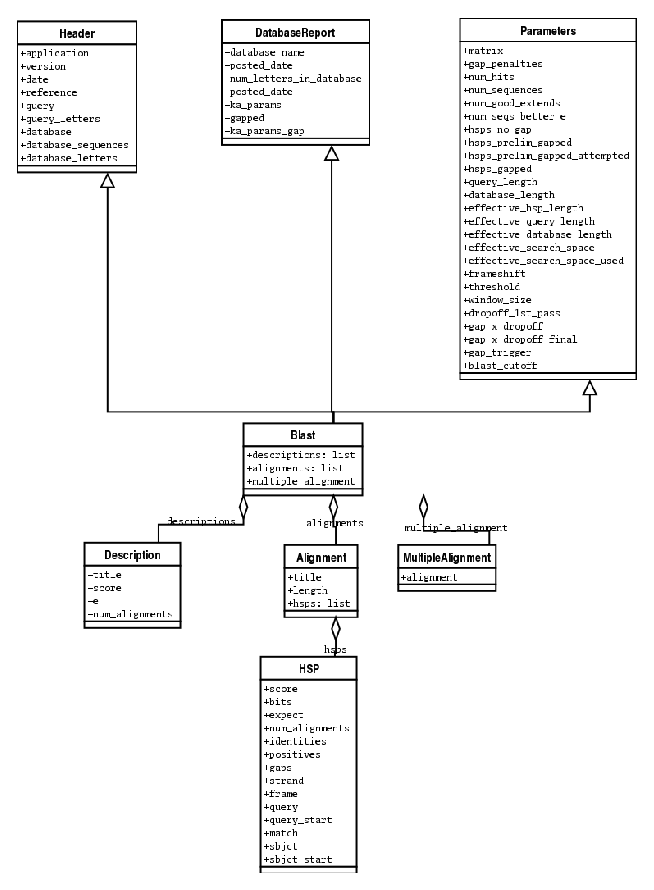
\includegraphics[width=0.8\textwidth]{images/BlastRecord}
\caption{BLAST �Υ�ݡ�����ξ����ɽ�����Ƥ��� Blast Record �Υ��饹��}
\label{fig:blastrecord}
\end{figure}
%\end{latexonly}


\class{PSIBlast} �쥳���ɥ��֥������Ȥ��ɤ����Ƥ��ޤ�����
\program{PSIBlast} �η����֤��Υ��ƥåפ��Ѥ����� \var{rounds}
�򥵥ݡ��Ȥ��Ƥ��ޤ���\class{PSIBlast} �Υ��饹�ޤ��
\ref{fig:psiblastrecord} �˼����ޤ���

%\begin{htmlonly}
%\label{fig:psiblastrecord}
%\imgsrc[width=650, height=750]{images/PSIBlastRecord.png}
%\end{htmlonly}

%\begin{latexonly}
\begin{figure}[htbp]
\centering
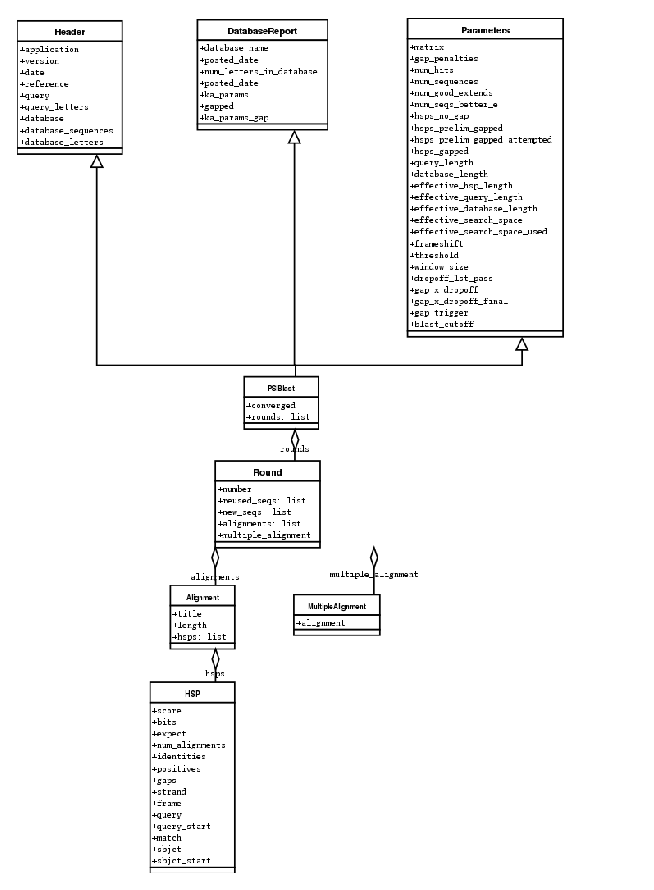
\includegraphics[width=0.8\textwidth]{images/PSIBlastRecord}
\caption{PSIBlast Record ���饹�Υ��饹��}
\label{fig:psiblastrecord}
\end{figure}
%\end{latexonly}

\subsection{��������� BLAST �����餻��}

����򸡺������оݤȤʤ�ǡ����١����򼫺�����ʤ顤��������Ǥ�
\program{BLAST} �μ¹Ԥ��ޤ��ˤ�����ˡ�Ǥ�������饤��Ǥ�
\program{BLAST} ��Ʊ�͡�Biopython �Ǥϥ�����ץȤ����������� 
\program{BLAST} �¹Է�����ƤӽФ��������餷�������ɤ������󶡤��Ƥ��ꡤ
\program{BLAST} �¹Է������󶡤��Ƥ����¿���Υ��ޥ�ɥ饤�󥪥ץ����
�����ƥ��������Ǥ���褦�ˤʤäƤ��ޤ���
�͡��ʥץ�åȥե���������Υ���ѥ���ѤߤΥ�������¹���
\program{BLAST} �ϡ�
\url{ftp://ncbi.nlm.nih.gov/blast/executables/} �Ǽ������ޤ���
�ޤ���NCBI toolbox (\url{ftp://ncbi.nlm.nih.gov/toolbox/}) ����
��ʬ�ǥ���ѥ��뤷�Ƥ�����Ǥ��ޤ���

��������Ǥ�\program{BLAST} �¹Ԥ����뤿��Υ����ɡ��Ȥ�櫓
\function{blastall} ��\function{blastpgp} �Ȥ��ä��ؿ��ϡ�
\module{Bio.Blast.NCBIStandalone} �ˤ���ޤ��������δؿ���
����̾�������ץ������¹Է������б����Ƥ��ޤ���

�����δؿ���Ȥäƥ�������Υǡ����١������Ф���\program{blastall}
��¹Ԥ�����̤��֤����Ƥߤޤ��礦���ޤ���\program{blast} ��¹Ԥ��뤿
���ɬ�פʥѥ������ꤷ�Ƥ����ޤ��礦���ΤäƤ����ͤФʤ�ʤ��Τϡ�
(\program{formatdb} ���Ѱդ��Ƥ������Ϥ���) �����оݤȤ���ǡ����١���
�ؤΥѥ���������������������ä��ե�����ؤΥѥ���������
\program{blastall} �¹Բ�ǽ�����ؤΥѥ����̤�ɬ�פ�����ޤ���

\begin{verbatim}
import os

my_blast_db = os.path.join(os.getcwd(), 'at-est', 'a_cds-10-7.fasta')
my_blast_file = os.path.join(os.getcwd(), 'at-est', 'test_blast',
                             'sorghum_est-test.fasta')
my_blast_exe = os.path.join(os.getcwd(), 'blast', 'blastall')
\end{verbatim}

���ƤΥѥ������ꤷ���Τǡ�\program{blast} ��¹Ԥ��Ʒ�̤���Ф�
�����������ޤ�����������Ԥ�\program{blast} ��¹Ԥ��ޤ�:

\begin{verbatim}
from Bio.Blast import NCBIStandalone

blast_out, error_info = NCBIStandalone.blastall(my_blast_exe, 'blastn',
                                                my_blast_db, my_blast_file)
\end{verbatim}

���������\program{blast} �ץ��������Ф��� Biopython ��
���󥿥ե������ϡ���Ĥ��ͤ��֤��Ƥ��뤳�Ȥ����դ��Ƥ���������
�ǽ������ͤ�\program{blast} �ν��Ϥ��Ф���ϥ�ɥ�ǡ�
��¸������ѡ������Ϥ�����Ǥ��ޤ�������ܤ�����ͤϡ�\program{blast}
���ޥ�ɤ��������뤳�Ȥ����륨�顼���Ϥ�����ޤ���

���顼����μ�갷�������Ǥ����Ȥ����Τϡ����顼��¸�ߤ��ʤ�����
\code{error_info.read()} ��¹Ԥ��褦�Ȥ���ȡ�\function{read}
�ν������֥��å�����Ƥ��ޤä��ͤ��֤��ʤ�����˥�����ץȤ�
��ߤ��Ƥ��ޤ�����Ǥ�����ιͤ��Ǥϡ�\code{blast_out} ��
�֤��줿��̤���Ϥ��Ƥⲿ�������ʤ��ä����ˤΤߥ��顼��
���Ϥ�������ʳ��ξ��ˤϲ��⤻���ۤ��äƤ����Τ������顼��
���ޤ���갷�����֤�����ˡ�Ǥ���

��̤���Ϥ������˥ե��������¸���Ƥ������ȻפäƤ���ʤ顤
���� WWW \program{blast} ����򻲾Ȥ��ơ�\module{copy} �⥸�塼���
�Ȥ����ˤĤ���Ĵ�٤Ƥ������ɤ��Ǥ��礦��

���ơ����Ϥ�������ä��Τǡ����β��Ϥ�Ԥ�ͤФʤ�ޤ���͡�
�Ǥ�����ɤ߿ʤ�ǡ���������Ǽ¹Ԥ���\program{BLAST} �ν��Ϥ���Ϥ���
��ˡ�ˤĤ��ƳؤӤޤ��礦��

\subsection{�������� BLAST �ν��Ϥ���Ϥ���}

�������� \program{BLAST} ������������Ϥϡ�web �١�����\program{BLAST}
�ν��ϤȤϰ�äƤ���Τǡ�\module{Bio.Blast.NCBIStandalone} ���äƤ���
�ѡ�����ȤäƷ�̤�������ޤ���

WWW blast �ξ���Ʊ�� (���Ҥξ���򻲾Ȥ��Ƥ�������)��
�ѡ����˽��Ϥ��Ϥ��ˤϡ��ϥ�ɥ륪�֥������Ȥ���äƤ��ʤ����
�ʤ�ޤ��󡥥ϥ�ɥ륪�֥������Ȥ� \function{readline} �᥽�åɤ�
�������Ƥ��ơ��������������ν�����ԤäƤ���ʤ���Фʤ�ޤ���
���������ϥ�ɥ�����뤿��ˤ褯�Ȥ�������ϡ�\function{blastall}
��\function{blastpgp} �Τ褦�ʡ�Biopython ���󶡤��Ƥ���ؿ���Ȥä�
��������\program{BLAST} ��¹Ԥ��뤫��\program{blast} ��
���ޥ�ɥ饤��ǥ�������˼¹Ԥ��ơ��ʲ��Τ褦�ʥ����ɤ�¹Ԥ��ޤ�:

\begin{verbatim}
blast_out = open('my_file_of_blast_output', 'r')
\end{verbatim}

WWW \program{blast} ��Ʊ���褦�ˡ��̤� Biopython ���ص��ؿ���
�虜�虜�Ȥ�ɬ�פϤ���ޤ���

���ơ��ϥ�ɥ뤬������ä��Τǡ�(�ʸ夳��� \code{blast_out} ��
�Ƥ֤��Ȥˤ��ޤ�) �����Ϥ���Ϥ���������Ǥ��ޤ��������Ϥβ��Ϥ�
�ʲ��Τ褦�ʥ����ɤǹԤ��ޤ�:

\begin{verbatim}
from Bio.Blast import NCBIStandalone

b_parser = NCBIStandalone.BlastParser()
b_record = b_parser.parse(blast_out)
\end{verbatim} 

���Υ����ɤ�¹Ԥ���ȡ�\program{BLAST} ������������ݡ��Ȥ���Ϥ��ơ�
\module{Blast} \class{Record} ���饹 (���Ϥ��Ƥ�����Ϥ�
���Ƥˤ�äơ�\class{Record} ���饹�� Blast �Ѥ� PSIBlast �Ѥ�
�ɤ��餫�ˤʤ�ޤ�) ������������������ǡ�������Ф���褦��
���Ƥ���ޤ����������Ǥϡ�������Ͱʾ�Υ��饤��������Ƥ��Ф���
��ñ�ʥ��ޥ����Ϥ��Ƥߤޤ���


\begin{verbatim}
E_VALUE_THRESH = 0.04
for alignment in b_record.alignments:
    for hsp in alignment.hsps:
        if hsp.expect < E_VALUE_THRESH:
            print '****Alignment****'
            print 'sequence:', alignment.title
            print 'length:', alignment.length
            print 'e value:', hsp.expect
            print hsp.query[0:75] + '...'
            print hsp.match[0:75] + '...'
            print hsp.sbjct[0:75] + '...'
\end{verbatim}

WWW �� �� BLAST �ˤ�������ϲ��ϤˤĤ��Ƥ���򤹤Ǥ��ɤ�Ǥ���С�
�嵭�����ɤ��������������Ƥ�Ʊ�����ȵ��Ť��Ǥ��礦�����餫��
���Ϥ���Ϥ��� \class{Record} ���饹�ˤ����顤��ϸ�����
\program{BLAST} �ν��Ϸ����˴ط��ʤ���갷����ΤǤ���
�ޤä��������餷����

�ְ�ĤΥ쥳���ɤ���ϤǤ���ΤϳΤ��ˤ��������ɡ�����������
�����쥳���ɤ����ä�\program{BLAST} ���ϥե�������ä���ä������͡�
-- ����äƤɤ���ä����������ϤǤ����?�׿��ۤ�̵�ѡ�������
������ˤ���ޤ���


\subsection{BLAST �ν��ϤǤ��äѤ��Υե��������Ϥ���}

����������������������ޤȤ�ˤ��ƥǡ����١��������ơ�
���Ƥ�������Ф��Ƥ褯�Ǥ�����ݡ��Ȥ���Ф���Ȥ������Ǥϡ�
�������� \program{blast} �Ϥ褯�Ǥ��Ƥ��ޤ���
�Ǥ����顤Biopython �ˤϡ��ϼ��Ǥ����ե��������������
Ǻ�ޤ��줺�˲��Ϥ��뵡ǽ������ޤ���

����ʥե�����β��Ϥϡ�blast ���ƥ졼�� (blast iterator)
���Ѥ��ƹԤ��ޤ������ƥ졼����Ȥ���褦�ˤ���ˤϡ��ޤ�
�ѡ��������ꤷ�ơ�blast �ν��ϥ�ݡ��Ȥ���Ϥ��� Blast 
\class{Record} ���֥������Ȥˤ��ޤ�:

\begin{verbatim}
from Bio.Blast import NCBIStandalone

b_parser = NCBIStandalone.BlastParser()
\end{verbatim}

���ˡ������췲�� blast �쥳���ɤ��Ф���ϥ�ɥ뤬�긵�ˤ����
���ꤷ�ơ������ \code{blast_out} �ȸƤ֤��Ȥˤ��ޤ���
�ϥ�ɥ�μ����ˤĤ��Ƥϡ���� blast ���Ϥβ��Ϥ˴ؤ������
�ܤ����Ҥ٤Ƥ��ޤ���

�ѡ�����ϥ�ɥ뤬������ä��Ȥ����ǡ��ʲ��Τ褦�ʥ��ޥ�ɤ�¹�
����С����ƥ졼��������Ǥ��ޤ�:

\begin{verbatim}
b_iterator = NCBIStandalone.Iterator(blast_out, b_parser)
\end{verbatim}

����ܤΥ��ץ����\code{b_parser} �ϥ��ץ����Ǥ���
�ѡ�������ꤷ�ʤ���С����Υ��ƥ졼�������� BLAST ��ݡ��Ȥ�
��İ���֤��Ƥ椭�ޤ���

���ƥ졼����������ä��顤(�ѡ�������������) blast �쥳���ɤ�
\function{next} �Ǽ��Ф��ޤ�:

\begin{verbatim}
b_record = b_iterator.next()
\end{verbatim}

���ƥ졼����\function{next} ��ƤӽФ����Ӥ˿������쥳���ɤ���
�֤��ޤ���
���ơ����Υ쥳�������Τˤ錄�ä�ȿ����� (iteration) ��Ԥ���
����������� blast ����ݡ��Ȥ�����Ǥ��ޤ�:

\begin{verbatim}
while 1:
    b_record = b_iterator.next()

    if b_record is None:
        break

    E_VALUE_THRESH = 0.04
    for alignment in b_record.alignments:
        for hsp in alignment.hsps:
            if hsp.expect < E_VALUE_THRESH:
                print '****Alignment****'
                print 'sequence:', alignment.title
                print 'length:', alignment.length
                print 'e value:', hsp.expect

                if len(hsp.query) > 75:
                    dots = '...'
                else:
                    dots = ''
                
                print hsp.query[0:75] + dots
                print hsp.match[0:75] + dots
                print hsp.sbjct[0:75] + dots
\end{verbatim}

�쥳���ɤ���Ϥ����äƤ��ޤ���\code{b_iterator.next()} ��
\code{None} ���֤����Ȥ����դ��Ƥ�������������ˤ�äơ�
�쥳���ɤ�¸�ߤ��뤫Ĵ�٤ʤ���\keyword{while} �롼�פ�¹Ԥ���С�
��ñ�˥ե��������Τˤ錄�ä�ȿ�������Ǥ��ޤ���

���ƥ졼����Ȥ��ȡ������оݤ���٤˰�ñ�̤Ť��ɤ߹���Τǡ������
blast �쥳���ɤ����������ʤ��˽����Ǥ��ޤ�����Ϥ���
��ǽ��ȤäƤȤ�Ǥ�ʤ��Ф��Ǥ����ե��������������ʤ�
���Ϥ������Ȥ�����ޤ���

\subsection{����ʥե������椫�������ʥ쥳���ɤ�õ��}

�������ƤȤƤ��Բ��˻פ�����ϡ������ BLAST �ե�����򤷤Ф餯��
�ֲ��Ϥ��Ƥ��ơ����θ�ѡ����� \exception{SyntaxError} ����ߤ���
�Ȥ�����ΤǤ�������Ͽ��������Ǥ����Ȥ����Τ⡤
\exception{SyntaxError} ���ѡ���������ʤΤ������뤤�� \program{BLAST}
������ʤΤ���ʬ����ʤ�����Ǥ�������˰������Ȥˡ����顼��̵�뤹��
���Ȥ���Ǥ��ޤ��󡥤Ȥ����Τ⡤�ɤ��Dz��Ϥ����Ԥ����Τ�Ƚ��ʤ��Τǡ�
���顼��̵�뤹��ȥǡ����ν��פʥݥ���Ȥ򸫲ᤴ���Ƥ��ޤ�����
����ʤ�����Ǥ���

���������������򤹤뤿��ˤϤ���äȤ���������ץȤ�񤫤ͤФʤ�ʤ�
�Τ���Ǥ����������� \module{Bio.Blast} �⥸�塼��ˤ�
\class{BlastErrorParser} �����ꡤ��Ȥ������˴�ñ�ˤ��Ƥ���ޤ���
\class{BlastErrorParser} �ϡ��̾�� \class{BlastParser} ��
���ˤ褯���Ƥ��ޤ������ѡ��������Ф���\exception{SyntaxError} 
����­���ơ�������ʬ�Ϥ��褦�Ȼ�ߤ�쥤�䤬�ɲä���Ƥ��ޤ���

���Υѡ����λȤ��������äȸ��Ƥߤޤ��礦 -- �ޤ��������оݤ�
�ե�����ȡ�ȯ����������Υ�ݡ��Ȥ�񤭽Ф�����Υե������������ޤ�:

\begin{verbatim}
import os
 
b_file = os.path.join(os.getcwd(), 'blast_out', 'big_blast.out')
error_file = os.path.join(os.getcwd(), 'blast_out', 'big_blast.problems')
\end{verbatim}

������\class{BlastErrorParser} ��ɬ�פˤʤ�ޤ�:

\begin{verbatim}
from Bio.Blast import NCBIStandalone

error_handle = open(error_file, 'w')

b_error_parser = NCBIStandalone.BlastErrorParser(error_handle)
\end{verbatim}

�ѡ������ϥ�ɥ�򥪥ץ����ΰ����Ȥ��Ƽ�äƤ��뤳�Ȥ�����
���Ƥ����������ϥ�ɥ���Ϥ��ȡ��ѡ�����\exception{SyntaxError}
�����Ф��� \program{blast} �����ƤΥ쥳���ɤ򤳤Υϥ�ɥ��
�񤭽Ф��ޤ����ϥ�ɥ�����ꤷ�ʤ���С����������쥳���ɤ�
��Ͽ����ޤ���

���ơ�\class{BlastErrorParser} ���̾��\program{blast} �ѡ�����
�褦�˻Ȥ��ޤ����Ȥ�櫓��\program{blast} �쥳�������Τˤ錄�ä�
���顼�ѡ�����Ȥäư�ĤŤĥ쥳���ɤ���Ϥ��뤿��˥��ƥ졼����
�������褦�Ȥ��Ƥ⤫�ޤ��ޤ���:

\begin{verbatim}
blast_out = open(b_file)
iterator = NCBIStandalone.Iterator(blast_out, b_error_parser)
\end{verbatim}

���˽Ҥ٤��褦�ˡ����������쥳���ɤϰ��٤˰�ĤŤ��ɤ߽Ф��ޤ���
�����������٤� \program{Blast} �˵������� (���ġ��ѡ������Τ�
�������ʤ�) ���顼����­���ơ�ɬ�פʽ�����Ԥ��ޤ�:

\begin{verbatim}
try:
    next_record = iterator.next()
except NCBIStandalone.LowQualityBlastError, info:
    print "LowQualityBlastError detected in id %s" % info[1]
\end{verbatim}

�����Ǥϡ�\class{BlastErrorParser} �ϰʲ��Τ褦�ʥ��顼�������Ǥ��ޤ�:


\begin{description}
\item [SyntaxError] -- �̾�� \class{BlastParser} ����������Τ�
Ʊ�����顼�ǡ��ѡ���������Υե��������ϤǤ��ʤ����Ȥ˵�������
���顼�Ǥ������Υ��顼���̾�ѡ����ΥХ������ȤäƤ���\program{BLAST}
�ΥС������ȡ��ѡ����������Ǥ���\program{BLAST} �ΥС�������
�԰��פΤ����줫�������Ǥ���

\item [LowQualityBlastError] -- �Ҥɤ��ʼ��ΰ������� 
(�㤨�С�����Ū��ñ��γ˻���Ϣ�ʤ꤫�鹽������Ƥ���褦��û������)
�� BLAST �˳ݤ��褦�Ȥ���ȡ�\program{BLAST} ���������Τ�ޥ�������
���ޤ������Ū�˲����оݤ�����ʤ��ʤäƤ��ޤ����Ȥ�����ޤ���
���ξ�硤���Ƥ����ڤ줿��ݡ��Ȥ����Ϥ��졤�ѡ�����
\exception{SyntaxError} ��Ф��Ƥ��ޤ��ޤ��������������ˤ�
\exception{LowQualityBlastError} �����Ф��ޤ������Υ��顼�ϡ�
�ʲ��Τ褦�ʹ��ܤ򥨥顼����Ȥ����֤��ޤ�:
  \begin{description}
    \item [\code{item[0]}] -- ���顼��å������Ǥ���
    \item [\code{item[1]}] -- ���顼�θ����Ȥʤä����ϥ쥳���ɤ� id 
�Ǥ������ι��ܤϡ����������������Ƥ���쥳���ɤ����Ƶ�Ͽ����
�����������ˤȤƤ�ͭ�ѤǤ���
  \end{description}
\end{description}

��˽Ҥ٤��褦�ˡ����顼��������ȡ�\class{BlastErrorParser} ��
����򵯤����Ƥ���쥳���ɤ�\code{error_handle} �˽񤭽Ф��ޤ���
����\code{error_handle} �����Ƥ�Ĵ�٤ơ���ʬ�λפä��褦�������
�����Ǥ��ޤ���ñ��� \program{blast} ��ݡ��Ȥ�Ȥäƥѡ�����
�ǥХå��Ǥ���Ǥ��⤷��ޤ��󤷡�blast �μ¹Ԥ������Ƥ����꤬
���Ĥ��뤫���Τ�ޤ��󡥤�����ˤ��Ƥ⡤�����餯ͭ�յ����θ���
�ʤ뤳�ȴְ㤤�ʤ��Ǥ�!

\class{BlastErrorParser} ��Ȥ��С������ \program{blast} �ե������
�ǥХå�����������äȳڤˤʤ�Ϥ��Ǥ���


\subsection{PSIBlast ���}

\program{PSIBlast} �򥹥���ץȤ����ñ��ľ�����Ǥ���褦�ˤ���
�ˤϡ�(���饤����ȷ�̤��顤Ŭ�ڤʷ����� align �ե��������Ϥ褦��)
�����ɤ򿧡��Ƚ񤤤Ƥ����ͤФʤ�ޤ��󡥤ޤ��� \program{PSIBlast} ��
�褯Ĵ�٤ơ����ޤ������ˡ��פ��Ĥ�ɬ�פ�����ޤ�...

% 
\section{SWISS-PROT}
\label{sec:swiss-prot}

\subsection{SWISS-PROT �Υ쥳���ɤ����ꤹ��}

SwissProt (\url{http://www.expasy.ch/sprot/sprot-top.html}) ��
����ѥ�����Υǡ����١����ǡ��������ƤϿͼ�ˤ�ä��Խ�����Ƥ��ޤ���
������ץȤ��� SWISS-PROT ����³������ˡ�ȡ�
SWISS-PROT �������֤�����̤�ʸ���Ϥ�����ˡ�򸫤Ƥߤޤ��礦��

�ǽ�ˡ���ʸ���Ϥ����оݤΥǡ����򤤤��Ĥ����Ф��Ƥ���ɬ�פ�����ޤ���
���Υ��륳��������� (chalcone synthase) �����ܤ��Ƥ���Ȥ��ޤ��礦
(�ʤ���̣�����������˵��褦�Ȥ��Ƥ��뤫�� ~\ref{sec:orchids} ��
���Ȥ��Ƥ�������)�����륳��������Ǥϡ���ʪ�Υե�ܥΥ��ɤ���������
�ط����Ƥ��ޤ����ե�ܥΥ��ɤ���ϡ������� UV �ݸ�ޤʤɤ�¿����
�����餷�����ʤ���������ޤ���

SwissProt �Ǹ�����Ԥ��ȡ����륳��������Ǥ˴ؤ�����ͳ��Υ���ѥ���
ID O23729, O23730, O23731 �����Ĥ���Ϥ��Ǥ���
�Ǥϡ�������ץȤ�񤤤ơ������Υ���ѥ��˴ؤ���ǡ��������ꤷ��
�ǡ�����ʸ���Ϥ������򤽤��ʾ������Ф��Ƥߤޤ��礦��

�ޤ��� \module{Bio.WWW.Expasy} �� \function{get_sprot_raw} �Ȥ����ؿ�
��ȤäƤ����Υ쥳���ɤ����ꤷ�ޤ���
���δؿ��ϤȤƤ������餷���� id �����Ϥ���ȡ����̤Υƥ����ȷ�����
�쥳���ɤ��֤��ޤ� (html �Ƕ�ϫ���ʤ��Ƥ��ߤޤ�!)��

��Ū�� 3 �ĤΥ쥳���ɤ������줿�顤1 �Ĥ��礭��ʸ����Ȥ��ƤޤȤᡤ
�Ĥ��ˤ���ʸ������ᤵ���ޤ������񤤤����Ȥ��Τ�Τ����ʲ��˼���
�����ɤǼ¸��Ǥ��ޤ�:

\begin{verbatim}
from Bio.WWW import ExPASy

ids = ['O23729', 'O23730', 'O23731']

all_results = ''
for id in ids:
    results = ExPASy.get_sprot_raw(id)
    all_results = all_results + results.read()
\end{verbatim}

���ơ�Expasy �Ǥθ�����̤����ꤷ���Τǡ����η�̤�ʸ���Ϥ��ƶ�̣��
���������Ф������������ޤ�����¾��¿���Υѡ�����Ʊ���褦�ˡ�
���ƥ졼���ȥѡ����򥻥åȥ��åפ��ޤ����������Ѥ���ѡ����� SwissProt
�ե������ʸ���Ϥ��ƥ쥳���ɥ��֥������Ȥ��Ѵ����ޤ����쥳���ɤǤϡ�
��̣���оݤȤʤ�°������ (feature) �����֥������Ȥ�°���ˤʤäƤ��ޤ�:

\begin{verbatim}
from Bio.SwissProt import SProt
from Bio import File

s_parser = SProt.RecordParser()
s_iterator = SProt.Iterator(File.StringHandle(all_results), s_parser)
\end{verbatim}

�ѡ����ǹ�ʸ���Ϥ�Ԥ����ˡ�ʸ����� \var{all_results} ��ϥ�ɥ�
(handle) ���Ѵ����Ƥ��뤳�Ȥ����դ��Ƥ������������ƥ졼�������ϥǡ���
���ԤŤ��ɤ߹����褦�ˤ��뤿��ˡ����ƥ졼���ˤϥϥ�ɥ���Ϥ��ͤ�
�ʤ�ޤ���
\module{Bio.File} �⥸�塼��ˤϡ�\function{StringHandle} �Ȥ����褯
�Ǥ��������ʴؿ������ꡤʸ�����ϥ�ɥ���Ѵ����Ƥ���ޤ���
�����餷��! ����ǡ��������Ф�������������ޤ�����

�������Ф�����ˡ����ƥ졼����Ȥäơ����ƤΥ쥳���ɤ���
���ɤ�ޤ��������Ǥϡ��ƥ쥳���ɤ��Ф��ơ�ñ�ˤ���äȤ������ޥ�����
ɽ�����ޤ��礦:

\begin{verbatim}
while 1:
    cur_record = s_iterator.next()

    if cur_record is None:
        break

    print "description:", cur_record.description
    for ref in cur_record.references:
        print "authors:", ref.authors
        print "title:", ref.title

    print "classification:", cur_record.organism_classification
    print
\end{verbatim}

��Υ����ɤϡ��ʲ��Τ褦�ʥ��ޥ����Ϥ��ޤ�:

\begin{verbatim}
description: CHALCONE SYNTHASE 8 (EC 2.3.1.74) (NARINGENIN-CHALCONE SYNTHASE 8)
authors: Liew C.F., Lim S.H., Loh C.S., Goh C.J.;
title: "Molecular cloning and sequence analysis of chalcone synthase cDNAs of
Bromheadia finlaysoniana.";
classification: ['Eukaryota', 'Viridiplantae', 'Embryophyta', 'Tracheophyta', 
'Spermatophyta', 'Magnoliophyta', 'Liliopsida', 'Asparagales', 'Orchidaceae', 
'Bromheadia']
\end{verbatim}

SwissProt �쥳���ɤ���¾�ξ������Ф�������С�Ʊ���褦�˴�ñ��
�Ԥ��ޤ���

\section{PubMed}
\label{sec:pub-med}

\subsection{PubMed �˥��������������}

���ʬ��뤤�ϥҥȤ˴ؿ�������ʤ� (���Ȥ������Ǥʤ��Ƥ⡤�ۤȤ�ɤ�
���!)��PubMed (\url{http://www.ncbi.nlm.nih.gov/PubMed/}) ��������
�����ͥ�줿���󸻤ˤʤ�Ǥ��礦���Ǥ����顤¾�ξ����Ʊ���褦�ˡ������Ǥ� 
Python ������ץȤ�Ȥäƾ����������ƻȤ���褦�ˤʤꤿ���Ǥ��͡�

Biopython ���Ѥ��� PubMed �˥����������Τϴ�ñ�Ǥ������˴ط��Τ���
���٤Ƥ�ʸ�� ID (article id) ����������С��ʲ��Τ��ä� 3 �ԤΥ�����
����ɬ�פ���ޤ���:

\begin{verbatim}
from Bio import PubMed

search_term = 'orchid'
orchid_ids = PubMed.search_for(search_term)
\end{verbatim}

���Υ����ɤϡ����˴ؤ��뤹�٤Ƥ�ʸ�� ID �� python �Υꥹ�ȤȤ���
�֤��ޤ�:


\begin{verbatim}
['11070358', '11064040', '11028023', '10947239', '10938351', '10936520', 
'10905611', '10899814', '10856762', '10854740', '10758893', '10716342', 
...
\end{verbatim}

���� ID �ꥹ�Ȥ������顤�ƥ쥳���ɤ������������ϴ�λ�Ǥ��������
�ʤߤޤ��礦��

\subsection{PubMed �Υ쥳���ɤ����ꤹ��}

����Ǥϡ���Ϣ�� ID �����������ˡ���������ޤ�����
ID �����ꤷ���顤���ϳ� ID �˴ط��Τ��� MEDLINE �Υ쥳���ɤ����ꤷ�ơ�
��������������Ф������ȹͤ���Ǥ��礦��

PubMed ����쥳���ɤ���Ф��륤�󥿡��ե������ϡ�Python �ץ�����ޡ���
�ȤäƤϤȤƤ�ľ��Ū�ʤϤ� -- Python �ˤ����뼭�񷿤Υ�ǥ벽 -- �Ǥ���
���Υ��󥿡��ե������򥻥åȥ��åפ���ˤϡ�PubMed �������������̤�
��ʸ���Ϥ��뤿��Υѡ�����ɬ�פǤ����ʲ��Υ����ɤǡ����ƤΥ��åȥ��å�
��Ԥ��ޤ�:

\begin{verbatim}
from Bio import PubMed
from Bio import Medline

rec_parser = Medline.RecordParser()
medline_dict = PubMed.Dictionary(parser = rec_parser)
\end{verbatim}

�����ǹԤä��Τϡ�����饤���ʥ��֥������Ȥ� \var{medline_dict} �κ���
�Ǥ���ʸ�����������ˤϡ�\code{medline_dict[id_to_get]} �Τ褦�ˤ���
�����������ޤ�����������Ԥ��ȡ� PubMed ����³����õ���Ƥ���ʸ����
���Ĥ���ʸ�������ʸ���Ϥ��ƥ쥳���ɥ��֥������Ȥ��Ѵ������֤��ޤ���
�ʤ�Ƹ�����Ǥ��礦! 


���ơ����������餷�����񥪥֥������Ȥ�ɤ��Ȥ��С����� ID ���餢�����
����ϤǤ��뤫���Ƥߤޤ��礦��ɬ�פʺ�Ȥϡ�ñ�˼긵�� ID (���������
���� \var{orchid_ids} �ˤˤ錄�äƥ롼�פ�����̣���оݤȤʤ�����ɽ��
��������Ǥ�:


\begin{verbatim}
for id in orchid_ids[0:5]:
    cur_record = medline_dict[id]
    print 'title:', string.rstrip(cur_record.title)
    print 'authors:', cur_record.authors
    print 'source:', string.strip(cur_record.source)
    print
\end{verbatim}

��Υ����ɤ��Ф�����Ϥϰʲ��Τ褦�ˤʤ�ޤ���

\begin{verbatim}
title: Sex pheromone mimicry in the early spider orchid (ophrys sphegodes):
patterns of hydrocarbons as the key mechanism for pollination by sexual
deception [In Process Citation]
authors: ['Schiestl FP', 'Ayasse M', 'Paulus HF', 'Lofstedt C', 'Hansson BS', 
'Ibarra F', 'Francke W']
source: J Comp Physiol [A] 2000 Jun;186(6):567-74
\end{verbatim}

��ɮ���٤��ϡ�����̾�Υꥹ�ȤǤ��������ɸ��� Python �ꥹ�ȷ��Ȥ���
�֤���Ƥ��ޤ����������뤳�Ȥǡ�Python ��ɸ��ġ����Ȥä�������
����������Ǥ��ޤ����㤨�С��ʲ��Τ褦�ʥ����ɤ�Ȥ��С���Ϣ�Υ���ȥ�
���Τˤ錄�äƥ롼�פ��ơ���������Ԥ�õ���Ф��ޤ�:


\begin{verbatim}
search_author = 'Waits T'

for id in our_id_list:
    cur_record = medline_dict[id]
    
    if search_author in cur_record.authors:
        print "Author %s found: %s" % (search_author,
                                       string.strip(cur_record.source))
\end{verbatim} 

PubMed �� Medline �Υ��󥿡��ե����������Ϥ����褯����Ƥ��ޤ� -- 
������ɤ�ǡ����äȤ��Υ��󥿥ե������ΰ��ϤȻȤ�����褯���򤷤�
��館�����ȤǤ��礦��

\section{GenBank}


GenBank �쥳���ɷ����ϡ����������˴ؤ���°������ (feature)��
����¾��Ϣ��������ξ����Ͽ������ˡ�Ȥ��ƹ����Ȥ��Ƥ��ޤ���
���η����ϡ�NCBI �Υǡ����١��� (\url{http://www.ncbi.nih.gov/}) 
�����������뤿����ɤ����ʤǤ⤢��ޤ���


\subsection{GenBank �Υ���ȥ�� NCBI �������ꤹ��}

\module{Bio.GenBank} �饤�֥�� �ΤȤƤ���Ũ�ʵ�ǽ�ϡ�����ȥ��
GenBank ���鼫ưŪ�˼����Ǥ���Ȥ����Ȥ����Ǥ���
����ϡ������κ�Ȥ�ư������褦�ʥ�����ץȤ�񤯾�ǤȤƤ�
�����Ǥ����������Ǥϡ�NCBI �ǡ����١����˥����������������������
����쥳���ɤ����ꤹ����ˡ�򼨤��ޤ���

�ޤ��ϥ������������ơ����Ф������쥳���ɤ��Ф��� ID �򸡺�
���ޤ��礦�������Ǥϡ���Τ����������\emph{�����掠�ܥƥ� (Opuntia)}
����˼�äơʤʤ��ʤ�䤬���椷�Ƥ��뤫��Ǥ��ˡ�����äȤ���������
�¹Ԥ��Ƥߤޤ��礦���ʲ��Υ����ɤ�Ȥ��С������å�������Ԥäơ�
���ƤΥ쥳���ɤ��б����� GI (GenBank ���̻�) ������Ǥ��ޤ�:

\begin{verbatim}
from Bio import GenBank

gi_list = GenBank.search_for("Opuntia AND rpl16")
\end{verbatim}

\var{gi_list} �ˤϡ�������˰��פ������٤Ƥ� GenBank ���̻Ҥ���ʤ�
�ꥹ�Ȥˤʤ�ޤ�:

\begin{verbatim}
['6273291', '6273290', '6273289', '6273287', '6273286', '6273285', '6273284']
\end{verbatim}

GI ������Ǥ����Τǡ��� ID ��ȤäƼ��񥤥󥿥ե�������𤷤� NCBI 
�ǡ����١����˥��������Ǥ��ޤ����㤨�С��ǽ�� GI ���Ф�������
��Ф���ʤ顤�ޤ� NCBI �˥����������뼭�񥪥֥������Ȥ���ʤ��Ƥ�
�ʤ�ޤ���:


\begin{verbatim}
ncbi_dict = GenBank.NCBIDictionary()
\end{verbatim}

���񥪥֥������Ȥ��ä��顤���Τ褦�˾������Ф��Ƥߤޤ��礦:

\begin{verbatim}
gb_record = ncbi_dict[gi_list[0]]
\end{verbatim}

������Ǥϡ�\var{gb_record} �� GenBank �����Υ쥳���ɤˤʤ�Ϥ��Ǥ�:

\begin{verbatim}
LOCUS       AF191665      902 bp    DNA             PLN       07-NOV-1999
DEFINITION  Opuntia marenae rpl16 gene; chloroplast gene for chloroplast
            product, partial intron sequence.
ACCESSION   AF191665
VERSION     AF191665.1  GI:6273291
...
\end{verbatim}

������Ǥϡ�ñ�����Υ쥳���ɤ����ꤷ�������Ǥ��������Υ쥳���ɤ�
ľ�ܥѡ������Ϥ��ƹ�ʸ���Ϥ������쥳���ɤ��Ѵ����뤳�Ȥ����ޤ���
�㤨�С� GenBank �ե����뤫����Ф��� \class{SeqFeature}
���֥������Ȥ� \class{SeqRecord} ���֥������Ȥ��ᤷ������С�
�ޤ�\module{GenBank} �� \class{FeatureParser} �Ǽ��񥪥֥������Ȥ�
��������ɬ�פ�����ޤ�:

\begin{verbatim}
record_parser = GenBank.FeatureParser()
ncbi_dict = GenBank.NCBIDictionary(parser = record_parser)
\end{verbatim}

����ǡ��쥳���ɤ���Ф���С��ǤΥƥ����ȷ����Υ쥳���ɤ�
����� \class{SeqRecord} ���֥������Ȥˤʤ�ޤ�:

\begin{verbatim}
>>> gb_seqrecord = ncbi_dict[gi_list[0]]
>>> print gb_seqrecord
<Bio.SeqRecord.SeqRecord instance at 0x102f9404>
\end{verbatim}

GenBank ����ɤ�ʷ������Ѵ��Ǥ��뤫�ˤĤ��Ƥξܺ٤ϡ�
\ref{sec:gb-parsing} ��򻲾Ȥ��Ƥ���������

����������ưŪ�������̼�����ǽ��Ȥ��ȡ����Ȥ���Ϥ뤫��ͭ���ˤ�
��ޤ������ξ塤������ǽ�ˤϰ�����֤��Ȥ˼�����Ԥ� time-delay �Τ褦
����Ũ�ʵ�ǽ���Ȥ߹��ޤ�Ƥ��ơ����ˤʥ��������ˤ�ä� NCBI ���ܤ餻��
����������֥��å������褦�ʤ��Ȥ��ʤ��褦�ˤ��Ƥ��ޤ���

\subsection{GenBank �쥳���ɤ��᤹��}
\label{sec:gb-parsing}

GenBank �ե�����������餷���Ǥ��Ƥ��ơ���������ξ��󤬤��������
��������ǡ��ºݤˤϰ���ˤۤ�ξ����ξ��󤷤����Ф������ʤ�����
����ޤ��󡥤���������Ȥθ��Ȥʤ�Τϡ��ǡ����򤤤��˹�ʸ���Ϥ��뤫��
����
Biopython �Ǥ�ʣ���� GenBank �ѡ������󶡤��Ƥ��ơ�����������Ȥ�
�Ԥ���Ǽ�����Ǥ���褦�ˤ��Ƥ��ޤ�������ޤǤΤȤ�����
\module{GenBank} �Ǥϰʲ��Υѡ������󶡤��Ƥ��ޤ�:


\begin{description}

\item [RecordParser] ���Υѡ������ǤΥ쥳���ɤ�ʸ���Ϥ��ơ� GenBank 
��ͭ�Υ쥳���ɥ��֥������ȷ������Ѵ����ޤ������Υ��֥������ȤǤ�
������ǤΥ쥳���ɤ����˶ᤤ��ǥ�ǰ����Τǡ�ñ�� GenBank ��
�ġ��Υ쥳���ɼ��Τ˶�̣��������ˤϤ��Υѡ�����Ȥ��Τ��褤�Ǥ��礦��

\item [FeatureParser] ���Υѡ������ǤΥ쥳���ɤ�\class{SeqRecord} 
���֥������Ȥ��Ѵ����ޤ���\class{SeqRecord} ���֥������ȤǤϡ�
���Ƥ�°���ơ��֥����\class{SeqFeatures} ��ɽ������Ƥ��ޤ�
(�����Υ��֥������ȤˤĤ��Ƥξܺ٤� \ref{sec:advanced-seq} ��
���Ȥ��Ƥ�������)�����ɸ��Ū�ʷ����Ǿ�������ꤷ�������ˤ�
������Υѡ�����Ȥ��Τ��褤�Ǥ��礦��

\end{description}

�ɤ������ˡ��Ȥ�ˤ��衤���������Υѡ����κǤ����Ū�ʻȤ����ϡ�
���ƥ졼����������ơ�GenBank �쥳���ɤ����ä��ե������ѡ�������
�Ȥ�����Τˤʤ�ޤ������κ�Ȥϡ�¾�Υǡ��������Ǥν�����ˡ������
���Ƥ��ơ��㤨�аʲ��Τ褦�ʥ����ɤˤʤ�ޤ�:


\begin{verbatim}
from Bio import GenBank

gb_file = "my_file.gb"
gb_handle = open(gb_file, 'r')

feature_parser = GenBank.FeatureParser()

gb_iterator = GenBank.Iterator(gb_handle, feature_parser)

while 1:
   cur_record = gb_iterator.next()

   if cur_record is None:
       break

   # now do something with the record
   print cur_record.seq
\end{verbatim}

���Υ����ɤǤϡ�ñ�� GenBank �ե�������Ϥä�ȿ��������Ԥ���
�쥳���ɤ��Ȥ˹�ʸ���Ϥ�Ԥä� SeqRecord �� SeqFeature ���֥������Ȥ�
�Ѵ��������Υ쥳���ɤ������ɽ�� \class{Seq} ���֥������Ȥ�
���Ϥ��ޤ���

¾�η�����Ʊ�͡�GenBank �쥳���ɤ򰷤��ġ��뤬�������󤢤�ޤ���
�����Υġ����Ȥ��� GenBank ��ȤäƤ�ꤿ�����Ȥϲ��Ǥ�Ǥ���
�Ϥ��Ǥ���


\subsection{����� GenBank �ǡ����١������������}

��ʬ�ѤθĿ�Ū�� GenBank �ǡ����١�����������ơ����񥪥֥������Ȥ�
�褦�˥��������Ǥ���Ȥ����ȤƤ������餷����ǽ������ޤ���
(����������餷��������ʵ�ǽ�Ǥ����Ȥ����Τϡ����Υ��������
�ǡ����١����ˤ⡤BioCorba ��Ȥäƥͥåȥ���ۤ��˥�������
�Ǥ��뤫��Ǥ� -- �ܺ٤� BioCorba �Υɥ�����Ȥ򻲾Ȥ��Ƥ�������)

��������ʥǡ����١����κ����Ǥϡ��ޤ�����ǥ����ե������������ơ�
�ե�������γƥ쥳���ɤ����᤯���������Ǥ���褦�ˤ��ޤ���
�����Ԥ��ˤϡ�\function{index_file} �ؿ���Ȥ��ޤ�:

\begin{verbatim}
>>> from Bio import GenBank
>>> dict_file = 'cor6_6.gb'
>>> index_file = 'cor6_6.idx'
>>> GenBank.index_file(dict_file, index_file)
\end{verbatim}

���κ�Ȥǡ� \file{my_index_file.idx} �Ȥ���̾���Υե����뤬����
����ޤ������ơ����Υ���ǥ�����Ȥ��С��ġ��Υ쥳���ɤ˥�������
�Ǥ���褦�ʼ��񥪥֥������Ȥ�����Ǥ��ޤ���
\class{Iterator} �� \class{NCBIDictionary} ���󥿥ե������Τ褦�ˡ�
�ǤΥ쥳���ɤ��ᤷ���ꡤ���񥪥֥������Ȥ�ѡ������Ϥ��ơ��쥳���ɤ�
�֤��������Ƥ�ʸ���Ϥ�������Ǥ��ޤ���
���ξ�硤�쥳���ɤ�������ˤ� \class{FeatureParser} ���Ϥ��Ƥ�����
���θ�� \class{SeqRecord} ���֥������Ȥ�������ޤ���

����ν����ϴ�ñ�ǡ��ʲ��� 1 �Ԥ����Ǥ�:

\begin{verbatim}
>>> gb_dict = GenBank.Dictionary(index_file, GenBank.FeatureParser())
\end{verbatim}

����ǡ�Genbank �Υǡ����򼭽����˰�����褦�ˤʤ�ޤ�����
�㤨��:

\begin{verbatim}
>>> len(gb_dict)
7
>>> gb_dict.keys()
['L31939', 'AJ237582', 'X62281', 'AF297471', 'M81224', 'X55053']
\end{verbatim}

�Ǹ�ˡ�ź��ɽ�� (subscripting) �ǥ��֥������Ȥ���Ф��ޤ�: 

\begin{verbatim}
>>> gb_dict['AJ237582']
<Bio.SeqRecord.SeqRecord instance at 0x102fdd8c>
\end{verbatim}
\section{���饤����Ȳ��Ϥΰ���}

��������󷲤��Ф��ƥ��饤����Ȥ�ݤ�����ȡ��ȤƤ������ʤ��Ȥ�
�褯����ޤ�����ԤϤ����褯�Ȥäơ���äĤ�Ū������֤δ�Ϣ����
Ĵ�٤��ꤷ�ޤ������äơ����饤����Ȥ�ݤ��ơ����η�̤����䤹��
���֥������Ȥ��֤��褦�� Python ������ץȤ򤹤Ф䤯�񤭾夲�����
�����ΤϤȤƤ������餷�����ȤʤΤǤ���Biopython �ˤ����륢�饤�����
��Ϣ�Υ����ɤϡ�Python ��٥뤫�饢�饤����Ȳ��ϥץ������˥�������
�Ǥ���褦�ˤ���������ץȾ夫������ᤤ���饤����Ȳ��Ϥ��ǽ��
���뤿��Τ�ΤǤ���

\subsection{clustalw}
\label{sec:align-clustal}

\program{clustalx}
(\url{http://www-igbmc.u-strasbg.fr/BioInfo/ClustalX/Top.html}) 
�ϡ��ޥ���ץ륢�饤����Ȥ�Ԥ������ͥ�줿�ץ������Ǥ���
Biopython �Ǥϡ�\program{clustalx} ���������� clustal �����Υ��饤����Ⱦ���
(�̾�ϳ�ĥ�� \file{*.aln} ���Ĥ��Ƥ��ޤ�) �˥����������뤿���
��ˡ���󶡤��Ƥ��ޤ����ޤ���\program{clustalx} �Υ��ޥ�ɥ饤���ǤǤ���
\program{clustalw} �ؤΥ����������ʤ��󶡤��Ƥ��ޤ���

\program{clustalw} �Ȥ��Ȥ��Ԥ���Ǥϡ��ޤ��ǽ�Υ��ƥåפȤ��ơ�
�ץ��������Ϥ����ޥ�ɥ饤����������ꤷ�ޤ��� \program{clustalw}
 �ˤ������
���Υ��ޥ�ɥ饤�󥪥ץ���󤬤��ꡤ��������Υѥ�᥿�����ꤹ�뤳�Ȥ�
�ʤ�С�����ʥ��ޥ�ɥ饤������Ϥˤ���˰���Ƥ��ޤ��Ǥ��礦��
���ޥ�ɥ饤�󥯥饹 (command line class) �Ǥϡ�����Ǥ���
���ޥ�ɥ饤�󥪥ץ����򥯥饹��°���Ȥ��ư������Ȥǡ����ޥ�ɥ饤��
���ǥ벽���Ƥ��ޤ�������Υѥ�᥿�����ꤹ�뤿����ص��ؿ���
�����Ĥ����ꡤ�ѥ�᥿����ˤ�����륨�顼�򸡽ФǤ���褦��
�ʤäƤ��ޤ���

\program{clustalw} �ˤ��ޥ���ץ륢�饤����Ȥ�¹Ԥ��뤿���
���ޥ�ɥ饤�󥪥֥������Ȥ��������ˤϡ��ʲ��Τ褦�ˤ��ޤ�:

\begin{verbatim}
import os
from Bio.Clustalw import MultipleAlignCL

cline = MultipleAlignCL(os.path.join(os.curdir, 'opuntia.fasta'))
cline.set_output('test.aln')
\end{verbatim}

�ޤ���\class{MultipleAlignCL} �� import ���ޤ������Υ��饹��
\program{clustalw} �ˤ��ޥ���ץ륢�饤����Ȥμ¹Ԥ��ǥ벽
���Ƥ��ޤ���
���ˡ����Υ��ޥ�ɥ饤�󥯥饹���������ޤ������κݡ�
���饤����Ȥ��оݤˤ��� FASTA �����Υե����������Ȥ���
���ꤷ�ޤ���
������ؿ��ˤϡ����ץ�������������Ȥ��ơ�\program{clustalw}
�μ¹ԥե����뤬����������Ǥ��ޤ����ǥե���ȤǤϡ�
\program{clustalw} ��\envvar{PATH} ��Τɤ����ˤ���Ȳ��ꤷ�ơ�
���ޥ�ɥ饤�󥪥֥������Ȥ�ñ�� \code{'clastalw'} �Ȥ���̾����
�ץ�������ƤӽФ��ޤ���

���ιԤǤϡ���̤ν������ե����� \file{test.aln} �����ꤷ�Ƥ��ޤ���
\class{MultipleAlignCL} ���֥������Ȥˤ�¾�ˤ⤿������Υѥ�᥿
�����ꡤ���Ϥη��������󥮥�åפΥ����ȤȤ��ä������Ԥ��ޤ���

���ޥ�ɥ饤������Ƥϡ�\class{MultipleAlignCL} ��\function{__str__} 
�᥽�åɤ�ƤӽФ�������������ɤ�ޤ����ºݤˤϡ�\code{str(cline)}
�Ȥ����ꡤñ�� \code{print cline} �Ȥ��������ɽ������ޤ���
�����Ǥϡ��ʲ��Τ褦�ʽ��Ϥˤʤ�Ϥ��Ǥ�:

\begin{verbatim}
clustalw ./opuntia.fasta -OUTFILE=test.aln
\end{verbatim}

���ơ���ñ�ʥ��ޥ�ɥ饤�������Ǥ����Τǡ����Υ��ޥ�ɥ饤���
�¹Ԥ��Ʒ�̤���ޤȤᡤ�����Ǥ���褦�ˤ��ޤ��礦��
�������ϡ�\class{Clastalw} ��\function{do_alignment} ��Ȥä�
�ʲ��Τ褦�˹Ԥ��ޤ�:

\begin{verbatim}
from Bio import Clustalw

alignment = Clustalw.do_alignment(cline)
\end{verbatim}

���¹Ԥ���ȡ�Biopython ����ۤ����ꤷ�����ޥ�ɥ饤���¹Ԥ��ơ�
����Υѥ�᥿�� \program{clustalw} �����餻�ޤ�������
\program{clustalw} ����ν��Ϥ�����ߡ�Biopython �����ϤǤ���
���� (���ߤΤȤ��� clustal �����Τ�) �Ǥ���С����Ϥ�Ԥäơ�
Ŭ�ڤʷ��Υ��饤����ȥ��֥������Ȥˤ����֤��ޤ��������Ǥϡ�
��̤�ǥե���Ȥ� clustal �����ˤ��Ƥ���Τǡ�����ͤΥ��֥�������
\code{alignment} ���֥������Ȥ� \class{ClustalAlignment} ���ˤʤ�ޤ���

\code{alignment} ���֥������Ȥ������顤�㤨�Х��饤��������
���Ƥ�������Ф���\class{seq_record} ���֥������Ȥ�����Ȥ��ä�
�褦�ʽ�����Ԥ��ޤ�:

\begin{verbatim}
all_records = alignment.get_all_seqs()

print 'description:', all_records[0].description
print 'sequence:', all_records[0].seq
\end{verbatim}

��Υ����ɤ�¹Ԥ���ȡ����饤����Ȥκǽ�����󥪥֥������Ȥ�
�Ф������� (description) �����󥪥֥������Ȥ���Ϥ��ޤ�:

\begin{verbatim}
description: gi|6273285|gb|AF191659.1|AF191
sequence: Seq('TATACATTAAAGAAGGGGGATGCGGATAAATGGAAAGGCGAAAGAAAGAAAAAAATGAAT 
...', IUPACAmbiguousDNA())
\end{verbatim}

���饤����Ȥκ���Ĺ��׻��Ǥ��ޤ�:

\begin{verbatim}
length = alignment.get_alignment_length()
\end{verbatim}

���饤����ȥ��֥������Ȥ򥪥ꥸ�ʥ�η����ǽ��Ϥ�������С�
ñ�� \function{__str__} �˥���������������Ǥ����Ĥޤꡤ
\code{print alignment} ��¹Ԥ�������Ǥ��ޤ��ޤ���:


\begin{verbatim}
CLUSTAL X (1.81) multiple sequence alignment


gi|6273285|gb|AF191659.1|AF191      TATACATTAAAGAAGGGGGATGCGGATAAATGGAAAGGCGAAAGAAAGAA
gi|6273284|gb|AF191658.1|AF191      TATACATTAAAGAAGGGGGATGCGGATAAATGGAAAGGCGAAAGAAAGAA
...
\end{verbatim}

��������С����ꥸ�ʥ�ξ���˼��ä��뤳�Ȥʤ������饤����ȷ�̤�
�ե�����˴�ñ�˽��᤻�ޤ���

���饤����ȷ�̤�Ȥä�¾�ˤ⤤�������ʤ��Ȥ򤷤Ƥߤ�����С�
���饤����ȷ�̤�\class{SummaryInfo} ���֥�������
�Τ褦�ʥ��饤����Ⱦ����������֥������Ȥ��Ϥ��Τ��٥��ȤǤ���
����ˤĤ��Ƥ�\ref{sec:summary-info} ����������ޤ���

\subsection{���ޥ����λ���}
\label{sec:summary-info}

���饤����ȷ�̤������顤���Ϥ�������������Ф����Ȥ���
�Ϥ��Ǥ��͡�Biopython �Ǥϡ����륢�饤����Ⱦ���˴ؤ������Ƥξ����
��������褦�ʰ�Ϣ�δؿ������ƥ��饤����ȥ��֥������Ȥ˻�������
����ˡ�����������ǽ�򥢥饤����ȥ��֥������Ȥ���������̤�
���饹��ʬΥ���褦�Ȼ�ߤƤ��ޤ���

���饤����ȥ��֥������Ȥ��饵�ޥ����򻻽Ф�������ϤȤƤ�
��ñ�Ǥ����㤨�С�\code{alignment} �Ȥ���̾���Υ��֥������Ȥ�
����Ȥ��ޤ��礦�����ޥ����򻻽Ф��륪�֥������Ȥ�������ɬ�פʤΤ�
��������Ǥ�:

\begin{verbatim}
from Bio.Align import AlignInfo
summary_align = AlignInfo.SummaryInfo(alignment)
\end{verbatim}

\code{summary_align} �ϤȤƤ������ʥ��֥������Ȥǡ��ʲ��Τ褦��
����������������ԤäƤ���ޤ�:

\begin{enumerate}
  \item ��ñ�ʥ��󥻥󥵥�����η׻� -- \ref{sec:consensus} �Ỳ��
  \item �����ð�Ū���������� (position specific score matrix) �η׻�
    -- \ref{sec:pssm} �Ỳ��
  \item �����̤η׻� -- \ref{sec:getting-info-content} �Ỳ��
  \item �Ĵ��ִ���������� -- ���ε�ǽ��
    �Ȥä��ִ���������ˡ�ξܺ٤�\ref{sec:sub-matrix} �Ỳ��
\end{enumerate}

\subsection{��ñ�ʥ��󥻥󥵥�����η׻�}
\label{sec:consensus}

\ref{sec:summary-info} ��Dz��⤵��Ƥ���\class{SummaryInfo} 
���֥������ȤǤϡ����饤����Ȥˤ������ñ�ʥ��󥻥󥵥�����
��׻����뵡ǽ���󶡤��Ƥ��ޤ���\code{summary_align} �Ȥ���̾����
\class{SummaryInfo} ���֥������Ȥ����Ƥ���Ȥ��ơ����󥻥󥵥������
�׻��ϰʲ��Τ褦�ˤ��ƹԤ��ޤ�:


\begin{verbatim}
consensus = summary_align.dumb_consensus()
\end{verbatim}

̾������������褦�ˡ����δؿ����Ԥ��Τ������˴�ñ�ʥ��󥻥󥵥��׻�
�ǡ����󥻥󥵥���ʬ�γ��������ƤλĴ��ȹ礷���Ǥⶦ�����ι⤤�Ĵ��
�ͤ����� (�ǥե���Ȥ� 0.3) ���⤤�ͤ���ľ��ˡ����λĴ��
���󥻥󥵥�������ɲä��ޤ���
���ͤ�ã���ʤ���С�ۣ��ʻĴ��ɽ��ʸ���򥳥󥻥󥵥�������ɲ�
���ޤ�������ͤΥ��󥻥󥵥������ \class{Seq} ���֥������Ȥǡ�����
����ե��٥åȤϥ��󥻥󥵥��������Ȥ����������󤫤��¬���ޤ���
���äơ�\code{print consensus} ��¹Ԥ���ȡ��ʲ��Τ褦�ʽ��Ϥ�
�ʤ�Ϥ��Ǥ�:


\begin{verbatim}
consensus Seq('TATACATNAAAGNAGGGGGATGCGGATAAATGGAAAGGCGAAAGAAAGAAAAAAATGAAT 
...', IUPACAmbiguousDNA())
\end{verbatim} 

���ץ����Υѥ�᥿���Ϥ��ȡ�\function{dumb_consensus} ��ư���
Ĵ���Ǥ��ޤ�:

\begin{description}
\item[����] ���󥻥󥵥�����γ����ˤ����ơ�����λĴ�򥳥󥻥󥵥�
�Ȥ��ƺ��Ѥ��뤿���ɬ�פʻĴ�ζ������Ǥ����ǥե���Ȥ� 0.7 �Ǥ���

\item[ۣ��ʻĴ��ɽ��ʸ��] ۣ��ʻĴ��ɽ���˻Ȥ���ʸ���Ǥ���
�ǥե���Ȥ� \code{'N'} �Ǥ���

\item[���󥻥󥵥�����Υ���ե��٥å�] ���󥻥󥵥�����˻Ȥ�
����ե��٥åȤǤ�������ե��٥åȤ���ꤷ�ʤ���硤���饤�����
�оݤ�����Υ���ե��٥åȤ˴�Ť�����¬���Ԥ��ޤ���
\end{description}

\subsection{�����ð�Ū����������}
\label{sec:pssm}

�����ð�Ū���������� (PSSM, position specific score matrix) 
��Ȥ��ȡ����饤����Ȥξ���򥳥󥻥󥵥��Ȥϰ㤦��ˡ�ǽ���Ǥ���
�͡������Ӥ�ͭ�Ѥʤ��Ȥ�����ޤ���
����Ū�ˤϡ�PSSM ��\emph{�׿�}���� (count matrix) �Ǥ���
PSSM �Ǥϡ����饤����Ȥγƥ����ˤĤ��ơ��ƥ���ե��٥å�ʸ����
���������������פ��ޤ�����׷�̤ϡ����餫����ɽŪ�������
��¦�μ��ˤȤä�ɽ�����ޤ�����������ϥ��󥻥󥵥�����Ǥ��ޤ��ޤ��󤬡�
���饤��������Ǥ�դ�����ˤ�Ǥ��ޤ���

�㤨�С��ʲ��Υ��饤�����:

\begin{verbatim}
GTATC
AT--C
CTGTC
\end{verbatim}

�ξ�硤���� PSSM ��:

\begin{verbatim}
      G A T C
    G 1 1 0 1
    T 0 0 3 0
    A 1 1 0 0
    T 0 0 2 0
    C 0 0 0 3
\end{verbatim}

�Ȥʤ�ޤ���

\code{c_align} �Ȥ���̾���Υ��饤����ȥ��֥������Ȥ������
���ޤ��礦�����󥻥󥵥������¦�μ��ˤ��� PSSM ��׻�����ˤϡ�
�ޤ����饤����Ȥ��Ф��륵�ޥꥪ�֥������Ȥ�������ơ�
���󥻥󥵥������׻����ޤ�:

\begin{verbatim}
summary_align = AlignInfo.SummaryInfo(c_align)
consensus = summary_align.dumb_consensus()
\end{verbatim}

�����ǡ� PSMM ��������뤳�Ȥˤʤ�ޤ������׻�����ݤˤ�
ۣ��ʻĴ�\code{N} ��̵�뤹��褦�ˤ��ޤ�:


\begin{verbatim}
my_pssm = summary_align.pos_specific_score_matrix(consensus,
                                                  chars_to_ignore = ['N'])
\end{verbatim}

����������Ĥ���ޤ�:
Two notes should be made about this:

\begin{enumerate}
  \item ����ե��٥åȤθ�̩����ݻ����뤿��ˡ���μ��ˤϥ��饤�����
���֥������ȤǻȤ��Ƥ��륢��ե��٥å����ʸ���������ѤǤ��ޤ���
����å�ʸ���� PSSM �ξ�μ��ˤ�����ޤ���

  \item ��¦�μ���ɽ����������ˤϡ����󥻥󥵥��Ǥʤ���Τ��Ϥ��Ƥ�
���ޤ��ޤ����㤨�С����饤������������ܤ�����򤳤���ɽ��
��������С��ʲ��Τ褦�ˤ��ޤ�:

\begin{verbatim}
second_seq = alignment.get_seq_by_num(1)
my_pssm = summary_align.pos_specific_score_matrix(second_seq
                                                  chars_to_ignore = ['N'])
\end{verbatim}

\end{enumerate}

���̿���¹Ԥ���ȡ�\class{PSSM} ���֥������Ȥ��֤��ޤ�����ۤɤΤ褦��
PSSM ��ɽ������ˤϡ�ñ�� \code{print my_pssm} ��¹Ԥ��ޤ�����̤�:

\begin{verbatim}
    A   C   G   T
T  0.0 0.0 0.0 7.0
A  7.0 0.0 0.0 0.0
T  0.0 0.0 0.0 7.0
A  7.0 0.0 0.0 0.0
C  0.0 7.0 0.0 0.0
A  7.0 0.0 0.0 0.0
T  0.0 0.0 0.0 7.0
T  1.0 0.0 0.0 6.0
...
\end{verbatim}

�Τ褦�ˤʤ�ޤ���

PSSM �γ����Ǥˤϡ�\code{your_pssm[sequence_number][residue_count_name]} 
�Τ褦��ź������ǥ��������Ǥ��ޤ����㤨�С���� PSSM �ǡ�����ܤ�����
���Ф���Ĵ� \code{'A'} �Υ�����Ȥ�����ˤ�:


\begin{verbatim}
>>> print my_pssm[1]['A']
7.0
\end{verbatim}

�Τ褦�ˤ��ޤ���

���Τ褦�ˡ� PSSM ���饹�ι�¤�ϡ������ð�Ū����������γ����Ǥ�
�����������������򤭤줤�˽��Ϥ�����Ȥ��ä��������ñ�ˤǤ���
�褦�ˤʤäƤ��ޤ���

\subsection{������}
\label{sec:getting-info-content}

�ʲ��β����ˤ������������¸����ɽ����ǽ�������¬�٤ˡ�
������ξ����̤�����ޤ���

ʬ����ʪ�ؼԸ����˽񤫤줿ͭ�Ѥʾ��������������Ȥ��Ƥϡ�
\url{http://www.lecb.ncifcrf.gov/~toms/paper/primer/} ������ޤ���
���饤����Ȳ��Ϥ���Ū�Ȥ�����硤���󥻥󥵥�����䡤������ʬ�����
�����̤�Ĵ�٤뤳�Ȥˤʤ�ޤ���
�ޥ���ץ����󥢥饤������������Υ����ˤ���������̤η׻��ϡ�
�ʲ��μ��ǹԤ��ޤ�:


\begin{displaymath}
IC_{j} = \sum_{i=1}^{N_{a}} P_{ij} * log(\frac{P_{ij}}{Q_{i}}) 
\end{displaymath}

�����ǡ����줾����ѿ��ΰ�̣�ϰʲ��Τ褦�ˤʤäƤ��ޤ�:

\begin{description}
  \item [$IC_{j}$] -- ���饤�������� $j$ ���ܤΥ����ξ����̡�
  \item [$N_{a}$] -- ����ե��٥åȤ�������ʸ���ο���
  \item [$P_{ij}$] -- �������������ʸ�����и��������� (�㤨�С�
���륢�饤����ȤΤ��륫�����ǡ�G �� 6 ���� 3 ��и����Ƥ���С�
�����ͤ� 0.5 �Ǥ�)��
  \item [$Q_{i}$] -- �����ʸ���νи����٤δ����͡����ι�ϥ��ץ�����
���ꡤ���λȤ����ϥ桼���ˤ���ͤ��Ƥ��ޤ����ǥե���ȤǤϡ�
����ѥ�������Ф��ƤϾ�� 0.05���˻�������Ф��Ƥ� 0.25 ��ưŪ��
������Ƥޤ�������ϡ�������Ψʬ�ۤ��Ф��벾�����ڹԤ�ʤ�����
�����̤η׻����������ޤ������餫�λ�����Ψʬ�ۤ��ꤷ�������䡤
��ɸ��Υ���ե��٥åȤ�Ȥ��������ˤϡ��桼���� $Q_{i}$ ���ͤ�
�󶡤��ʤ���Фʤ�ޤ���
\end{description}

���ơ�Biopython �ǤɤΤ褦�˾����̤�׻����Ƥ��뤫�����򤷤��Ȥ����ǡ�
���饤����Ȥ�������ΰ���Ф��ƾ����̤�׻�������ˡ�򸫤Ƥ椭�ޤ��礦��

�ޤ������饤����ȥ��֥������Ȥ�Ȥäƥ��ޥꥪ�֥������Ȥ�������ޤ���
����̾���� \code{summary_align} �Ȥ��ޤ� (���ޥ�μ�����ˡ��
\ref{sec:summary-info} ��򻲾Ȥ��Ƥ�������) �����ޥꥪ�֥������Ȥ�
����줿�顤�����̤η׻��ϴ�ñ�Ǥ�:

\begin{verbatim}
info_content = summary_align.information_content(5, 30, 
                                                 chars_to_ignore = ['N'])
\end{verbatim}

�����á��񤷤����ʼ��ˤ��Ƥϡ�������ñ�˷׻��Ǥ��ޤ���! 
\code{info_content} �ˤϡ����ꤷ���ΰ� (���饤�������� 5 ���� 30 �ޤǤ�
��) �ˤ���������̤򼨤���ư�����������ͤ����äƤ��ޤ���
�����Ǥϡ������̤�׻�����Ȥ��ˤ����ޤ��ʻĴ� \code{'N'} ��̵�뤵����
���ޤ���������̾�Υ���ե��٥åȤ� \code{'N'} �����äƤ��ʤ�
����Ǥ���

��Ǥ⿨�줿�褦�ˡ��и����٤δ����ͤ�Ϳ��������о����̤�׻�
�Ǥ��ޤ�:

\begin{verbatim}
expect_freq = {
    'A' : .3,
    'G' : .2,
    'T' : .3,
    'C' : .2}
\end{verbatim}

���δ����ͤ��Ǥμ���ǤϤʤ���\class{SubMat.FreqTable} ���֥�������
(\class{FreqTable} �ξܺ٤� \ref{sec:freq-table} ��򻲾Ȥ��Ƥ�������) ��
�����Ϥ��ޤ���FreqTable ���֥������Ȥϡ�Biopython �� \class{Seq} ���饹
�ˤ����뤫�餯���Ʊ���褦�ˡ������\class{Alphabet} ���֥������Ȥ�
��Ϣ�Ť��뤿���ɸ����󶡤��Ƥ��ޤ���

\class{FreqTable} ���֥������Ȥνи����ټ��񤫤�κ����ϡ�
�ʲ��Τ褦�ˤ�������Ǥ�:

\begin{verbatim}
from Bio.Alphabet import IUPAC
from Bio.SubsMat import FreqTable

e_freq_table = FreqTable.FreqTable(expect_freq, FreqTable.FREQ,
                                   IUPAC.unambigous_dna)
\end{verbatim}

�и����٥ơ��֥뤬�������С����饤����Ⱦ���ΰ���Ф���
���о����̤η׻��Ϥ��Ȥ��ñ�Ǥ�:

\begin{verbatim}
info_content = summary_align.information_content(5, 30,
                                                 e_freq_table = e_freq_table,
                                                 chars_to_ignore = ['N'])
\end{verbatim}

���٤ϡ�\code{info_content} �ˤϻ��ꤷ���и����ٴ����ͤ˴�Ť�������
�����̤�����ޤ���

����ͤϡ������μ��Ǥ��п��δ���� 2 �Ȥ����׻��η�̤ˤʤ�ޤ���
�����ͤ�\var{log_base} �ѥ�᥿�˻Ȥ������ͤ���ꤷ���ѹ��Ǥ��ޤ�:

\begin{verbatim}
info_content = summary_align.information_content(5, 30, log_base = 10
                                                 chars_to_ignore = ['N'])
\end{verbatim}

����������Ǿ����̤η׻���Ǥ���褦�ˤʤ�ޤ������ºݤ�����ˤ��ξ�����
����Ѥ��Ƥߤ褦�ȹͤ��Ƥ���ʤ顤�ޤ��Ͼ����̤˴ؤ���ʸ���򷡤겼����
�ߤơ����λȤ�����ͤ��Ƥߤ�Ȥ褤�Ǥ��礦��Ĵ�٤���̡����δؿ��Υ����ɤ�
�񤯤Ȥ��˲��餫�δְ㤤���Ȥ��Ƥ������Ȥ��狼�ä��������Ȥ������Ȥ�
�ʤ��Ϥ��Ǥ����ɤ�!

\subsection{���饤����Ȥν��Ϸ������Ѵ�����}
\label{sec:align-translate}

�ۤʤ���Ϸ����֤��Ѵ���Ԥ�ʤ���Фʤ�ʤ��ʤꡤ�����ˤ���Ƥ��ޤ�
���Ȥ��褯����ޤ���Biopython �Ǥϡ����饤����ȥ��֥������Ȥ˴ؤ���
���������Ѵ��� \class{FormatConverter} ���饹�ǹԤäƤ��ޤ���
�ޤ������륢�饤����ȷ�̤� clustal �����Dz��Ϥ���
\class{ClustalAlignment} ���֥������ȤȤ��ƻ��äƤ���Ȥ��ޤ�:

\begin{verbatim}
import os
from Bio import Clustalw

alignment = Clustalw.parse_file(os.path.join(os.curdir, 'test.aln'))
\end{verbatim}

�����ǡ����Υ��饤����ȷ�̤� FASTA �������Ѵ����ޤ��礦���ޤ���
\class{FormatConverter} ���֥������� \code{converter} ��������ޤ�:

\begin{verbatim}
from Bio.Align.FormatConvert import FormatConverter

converter = FormatConverter(alignment)
\end{verbatim}

���� \code{converter} ���Ѵ����������饤����ȷ�̤��Ϥ��ޤ���
FASTA �������Ѵ���������аʲ��Τ褦�ˤ�������Ǥ�:

\begin{verbatim}
fasta_align = converter.to_fasta()
\end{verbatim}

�������������줿 \code{fasta_align} ���֥������Ȥ�
\code{print fasta_align} ����ɽ�����Ƥߤ�ȡ��ʲ��Τ褦�ˤʤ�ޤ�:

\begin{verbatim}
>gi|6273285|gb|AF191659.1|AF191
TATACATTAAAGAAGGGGGATGCGGATAAATGGAAAGGCGAAAGAAAGAATATATA----
------ATATATTTCAAATTTCCTTATATACCCAAATATAAAAATATCTAATAAATTAGA
...
\end{verbatim}

��������Ѵ��β����Ǥϡ�����η�����ͭ�ξ��󤬼����Ƥ��ޤ����Ȥ�
����ޤ����ȤϤ��������饤����Ȥ˴ؤ������Ū�ʾ���ΤۤȤ�ɤ�
�Ĥ����Ϥ��Ǥ���

���衤�͡��ʷ����Υ��ݡ��Ȥ��ɲä����ˤĤ졤����С������͡��ʷ�����
�ɤ߽񤭤Ǥ���褦�˲��ɤ���Ƥ椯�Ϥ��Ǥ���

\section{�ִ�����}
\label{sec:sub-matrix}

�ִ����� (substitution matrix) �ϡ��Х�������ե��ޥƥ�������
�ؤ��������κ�ȤǤ����ƽ��פ���ʬ�ȤʤäƤ��ޤ���
�ִ�����ϡ���ĤλĴ�δ֤��ߤ��ˤɤ줯�餤�ִ�����䤹������
ʬ�ह��ݤ˥������դ�����ˡ���󶡤��ޤ���
�ִ�����Ϥޤ����������Ӥ������Բķ�Ǥ���
Durbin ¾�ν񤤤� ``Biological Sequence Analysis'' �Ȥ����ܤˤϡ�
�ִ�����˴ؤ���ͥ�줿�Ҳ�Ȥ��λȤ������񤫤�Ƥ��ޤ���
�ִ������ͭ̾�ʤ�Τˤ� PAM �� BLOSAM ���󤬤���ޤ���

Biopython �Ǥϡ��褯�Ȥ��Ƥ����ִ�����򤿤������󶡤��Ƥ��Ƥ��ޤ���
�ޤ���������ִ���������������ʤ��󶡤��Ƥ��ޤ���

\subsection{�����Ȥ��Ƥ����ִ������Ȥ�}

\subsection{���饤����Ȥ����ִ�����򼫺��}
\label{sec:subs-mat-ex}

�ִ����󥯥饹�������餷����ǽ�ΰ�Ĥˡ����饤����Ȥ����
�ִ����������������ޤ����ºݤˤϡ��ִ�����������ϥ���ѥ���
���󥢥饤����Ȥ���Ԥ��Τ����̤Ǥ������������Ǥϡ�
�ޤ� Biopython �Υ��饤����ȥ��֥������Ȥ�������ơ�
���饤����Ȥξ���򻻽Ф��륵�ޥꥪ�֥������Ȥ����ޤ�:

\begin{verbatim}
from Bio import Clustalw
from Bio.Alphabet import IUPAC
from Bio.Align import AlignInfo

# Clustalw �Υ��饤����ȷ�̤��饢�饤����ȥ��֥������Ȥ�����
c_align = Clustalw.parse_file('protein.aln', IUPAC.protein)
summary_align = AlignInfo.SummaryInfo(c_align)
\end{verbatim}

��Υ����ɤ˴ؤ���ܤ��������\ref{sec:align-clustal} ���
\ref{sec:summary-info} ��ˤ���ޤ���

���ơ�\code{summary_align} ���֥������Ȥ�������ä��Τǡ�
�����Ȥäơ�����֤ǰۤʤ�Ĵ�ؤ��֤����������ٵ����Ƥ��뤫
Ĵ�٤뤳�Ȥˤ������Ȼפ��ޤ���������ɤߤ䤹����Τˤ��뤿��ˡ�
����¦�� (polar charged side chain) ����ä����ߥλ�������
���ܤ��ޤ��礦�������ʤ��Ȥˡ����κ�Ȥϡ�̵�뤷�����Ĵ��ɽ��ʸ��
���Ƥ��Ϥ��� (���ץ����� \var{skip_chars} �����ꤷ�Ƥ��뤳�Ȥ�
�ʤ�ޤ�) ʸ���ִ����� (replacement dictionary) ���������д�ñ��
�Ԥ��ޤ��������ǡ��������ߥλ��������оݤˤ���褦��ʸ���ִ������
�ʲ��Τ褦�ˤ��ƺ������ޤ�:

\begin{verbatim}
replace_info = summary_align.replacement_dictionary(["G", "A", "V", "L", "I",
                                                     "M", "P", "F", "W", "S",
                                                     "T", "N", "Q", "Y", "C"])
\end{verbatim}

\code{replace_info} �ϥ��ߥλ��Ĵ���ִ��˴ؤ������ǡ�Python ����
�Ȥ���ɽ������Ƥ��ơ����Ƥϰʲ��Τ褦�ˤʤäƤ��ޤ�:

\begin{verbatim}
{('R', 'R'): 2079.0, ('R', 'H'): 17.0, ('R', 'K'): 103.0, ('R', 'E'): 2.0, 
('R', 'D'): 2.0, ('H', 'R'): 0, ('D', 'H'): 15.0, ('K', 'K'): 3218.0, 
('K', 'H'): 24.0, ('H', 'K'): 8.0, ('E', 'H'): 15.0, ('H', 'H'): 1235.0, 
('H', 'E'): 18.0, ('H', 'D'): 0, ('K', 'D'): 0, ('K', 'E'): 9.0, 
('D', 'R'): 48.0, ('E', 'R'): 2.0, ('D', 'K'): 1.0, ('E', 'K'): 45.0, 
('K', 'R'): 130.0, ('E', 'D'): 241.0, ('E', 'E'): 3305.0, 
('D', 'E'): 270.0, ('D', 'D'): 2360.0}
\end{verbatim}

���ξ���ϡ����饤����Ȥκݤ˥��ߥλ��ִ��Ȥ��Ƶ��Ƥ����Ĵ����
���뤤������֤��͡��ʻĴ���ִ����ɤ���������ꤦ�뤫�򼨤��Ƥ��ޤ���
��ɤΤȤ�������Ȥ���˿ʤ���ִ���������������ɬ�פʾ����
��������Ǥ����ޤ��������ִ�����ξ����Ȥäơ�
�����ִ����� (ARM: Accepted Replacement Matrix) ��������ޤ�:

\begin{verbatim}
from Bio import SubsMat
my_arm = SubsMat.SeqMat(replace_info)
\end{verbatim}

���μ����ִ������Ȥäơ���Ȥ򤵤�˿ʤ���п���Ψ����
(log odds matrix)�����ʤ��ɸ�෿���ִ����� (Substitution Matrix) ��
�������ޤ�:

\begin{verbatim}
my_lom = SubsMat.make_log_odds_matrix(my_arm)
\end{verbatim}

�п���Ψ����κ����ϡ��ʲ��Τ褦�ʥ��ץ��������ǥ������ޥ���
�Ǥ��ޤ�:

\begin{description}
  \item [\var{exp_freq_table}] -- �ƥ���ե��٥åȤνи����٤�
�����ͤ��Ϥ��ޤ��������ͤ��Ϥ��ȡ��ִ��δ����ͤ�׻�����ݤ�
accepted replacement matrix ������˻Ȥ��ޤ���

  \item [\var{logbase}] -- �п���Ψ�������������Ȥ����п���
��Ǥ����ǥե���Ȥ��ͤ� 10 �Ǥ���

  \item [\var{factor}] -- �п���Ψ����γƥ���ȥ�˳ݤ�����
��Ψ�Ǥ����ǥե���Ȥ��ͤϡ�������ο��������䤹���ʤ�褦 10 ��
���ꤵ��Ƥ��ޤ���

  \item [\var{round_digit}] -- ��������ͤ򾯿��貿�̤ޤǴݤ�뤫��
ɽ�����Ǥ����ǥե���Ȥ��ͤ� 0 (�������ʤ�) �Ǥ���

\end{description}

�п���Ψ����������顤\function{print_mat} ��ȤäƤ������Ƥ�����
ɽ���Ǥ��ޤ��������������������Ϥ���ȡ��ʲ��Τ褦�ˤʤ�ޤ�:

\begin{verbatim}
>>> my_lom.print_mat()
D   6
E  -5   5
H -15 -13  10
K -31 -15 -13   6
R -13 -25 -14  -7   7
   D   E   H   K   R
\end{verbatim}

�����餷��������ǡ��ޤ��˼�ʬ�Ѥ��ִ����������Ǥ��ޤ���!

\section{�����٤����󥯥饹 -- ���� ID �� Feature}
\label{sec:advanced-seq}

\ref{sec:sequence} ��Ǥϡ�Biopython ���󥯥饹�δ��ä����ƤˤĤ���
�ؤӡ������������򰷤������ʽ����ˤĤ����������ޤ�����
�ȤϤ���������ˤϡ��������ʳ��ˤ���פ� feature (����) ����Ϣ�դ�
���Ƥ��뤳�Ȥ��褯����ޤ���������Ǥϡ���������������Ф���
����ε��Ҥ򰷤���ˡ�ˤĤ��ƽҤ٤ޤ���

\subsection{���� ID �� Description -- SeqRecords �򰷤�}

��Ǹ����Ȥ��������󥯥饹�Ȥϡ��ºݤˤ� \module{Bio.SeqRecord}
�⥸�塼����������Ƥ��� \class{SeqRecord} ���饹�Ǥ���
���Υ��饹�Ǥϡ������ id ���������������˴�Ϣ�Ť�
�Ǥ���褦�ˤʤäƤ��ޤ������饹���ΤϤȤƤ�ñ��ǡ��ʲ��Τ褦��
����򥤥󥹥���°���η����󶡤��Ƥ��ޤ�:

\begin{description}
  \item[seq] -- ������ -- \module{Bio} �⥸�塼��� \class{Seq} 
���֥������ȤǤ���

  \item[id] -- ������̤���ݤ˻Ȥ��ץ饤�ޥ�� id �Ǥ���
�ۤȤ�ɤξ�硤������������ֹ�ʤɤ� id �ˤ��ޤ���

  \item[name] -- ����Ρְ���Ū�ʡ�̾��/id �Ǥ��������ͤ�
������������ֹ��Ʊ���ˤʤ뤳�Ȥ⤢����ޤ�������������̾��
�ʤäƤ��뤳�Ȥ⤢��ޤ�����Ϥ����ͤ� GenBank �쥳���ɤˤ�����
LOCUS id �Τ褦�ʤ�Τ��ȹͤ��Ƥ��ޤ���

  \item[description] -- ������Ф��롤�ʹ֤��ɤ��狼��פ�����ʸ
�Ǥ���FASTA �����Υ���ȥ�ǡ� id �θ����³�����Ƥ�Ʊ���褦�ʤ�ΤǤ���

  \item[annotations] -- �������°����򼭽�ˤ�����ΤǤ���
�ƾ����̾���������ˡ���������Ƥ��ͤˤʤäƤ��ޤ������μ����
�Ȥ����Ȥǡ�����Ρֹ�¤������Ƥ��ʤ��׾�����ɲäǤ��ޤ���

  \item[features] -- ����� feature �˴ؤ��빽¤�����줿����
�����ä�\class{SeqFeature} ���֥������Ȥ���ʤ�ꥹ�ȤǤ���
\class{SeqFeature} �ι�¤�ˤĤ��Ƥϲ���\ref{sec:seq-features}
�Ǿܤ����������ޤ���
\end{description}

\class{SeqRecord} ���饹�ˤ����Ƥξ���°���Ȥ�����¸����Ƥ��뤿�ᡤ
�Ȥ����Ϥ��ۤ��񤷤�����ޤ��󡥥��饹�ν�����ϡ�ñ�� \class{Seq}
���֥������Ȥ� \class{SeqRecord} ���Ϥ������Ǥ�:

\begin{verbatim}
>>> from Bio.Seq import Seq
>>> simple_seq = Seq("GATC")
>>> from Bio.SeqRecord import SeqRecord
>>> simple_seq_r = SeqRecord(simple_seq)
\end{verbatim}

����ˡ�������ؿ��ˤ� \var{id} �� \var{name}��\var{description}
�Ȥ��ä��ѥ�᥿��Ϳ�����ޤ����ѥ�᥿��Ϳ���ʤ����ˤϡ�
������������̤�ΤǤ��뤳�Ȥ򼨤�ʸ�������ꤵ��ޤ�������
�ͤϸ���ѹ��Ǥ��ޤ�:

\begin{verbatim}
>>> simple_seq_r.id
'<unknown id>'
>>> simple_seq_r.id = 'AC12345'
>>> simple_seq_r.description = 'My little made up sequence I wish I could 
write a paper about and submit to GenBank'
>>> print simple_seq_r.description
My little made up sequence I wish I could write a paper about and submit 
to GenBank
>>> simple_seq_r.seq
Seq('GATC', Alphabet())
\end{verbatim}

���Υơ��������ɲäϤȤƤ��ñ�ǡ�ñ�� \member{annotation} ����
��ľ����������Ǥ�:

\begin{verbatim}
>>> simple_seq_r.annotations['evidence'] = 'None. I just made it up.'
>>> print simple_seq_r.annotations
{'evidence': 'None. I just made it up.'}
\end{verbatim}

�Ф��뤳�ȤϤ�������Ǥ�! ���ϡ�����˴ؤ�������¤������
ɽ���Ǥ��� \class{SeqFeature} �ˤĤ����Τꤿ���ʤä����ȤǤ��礦��

\subsection{feature �ȥ��Υơ������ -- SeqFeature}
\label{sec:seq-features}

���������:feature �ϡ�����ε��Ҿ���פ���ʬ�����Ƥ��ޤ���
����ʳ��ξ��󤬼�����ä���硤��������������ȿ������ơ�
����ˤĤ���Ƚ�äƤ������������ݲ��פ������䤹������褦��
���ʤ�ɬ�פˤʤ�ޤ������⤫��򰷤���褦�����Ѥ����� feature ���饹
��ȯ����Τ��Բ�ǽ���⤷��ޤ��󤬡�Biopython ������ feature ���饹
�Ǥ�����˴ؤ�������Ǥ���¤ꥫ�ץ��벽���褦�Ȼ�ߤƤ��ޤ���
���� feature ���饹���߷פϡ�GenBank/EMBL �������ơ��֥�˶�����¸
���Ƥ���Τǡ��⤷ GenBank �� EMBL �������ɤ������ΤäƤ���С�
Biopython ������ feature ���饹���ɤ�������¤�ˤʤäƤ��뤫��ñ��
�İ��Ǥ���Ǥ��礦��

\subsubsection{SeqFeature ��}

���� feature �򰷤��ݡ�\class{SeqFeature} ���饹���Τ��ǡ�����¤�κǽ��
�ʳ��Ȥʤ�ޤ������Υ��饹�ˤ��͡���°��������Τǡ��ޤ���
���줾���°���Ȱ���Ū�ʵ�ǽ����󤷤ơ����θ�Ǽ���� GenBank ��
feature �ơ��֥��Ŭ�Ѥ�����ˡ�򼨤�����������򤤤Ƥ椯���Ȥ�
���ޤ��礦��\class{SeqFeature} ��°���ϰʲ��Τ褦�ˤʤäƤ��ޤ�:

\begin{description}
  \item[\member{location}] -- \class{SeqFeature} ��ɽ�� feature ��
�оݤˤ��Ƥ��������ΰ��֤Ǥ���\member{location} ��ü������Ϥ����ޤ��Ǥ�
���ޤ��ޤ��� -- \member{location} �򰷤���ˡ�ˤĤ��Ƥξܤ���������
\ref{sec:locations} �ˤ���ޤ���

  \item[\member{type}] -- feature �Υ����פ�ƥ����Ȥ�ɽ������ΤǤ�
(�㤨�Ф����ͤ� 'CDS' �� 'gene' �ˤʤ�ޤ�)��

  \item[\member{ref}] -- �̤�������Ф��뻲�ȤǤ������� feature �ϻ��ˡ�
��������Ρ־�ˡפ���ʤ��顤�̤�������Ф��뻲�Ȥ�ԤäƤ���
��礬����ޤ�������°���ϡ���������¾������� (�̾�ϥ����������
�ֹ��) ���Ȥ�����ʤ��󶡤��ޤ������������ʬ���������ΰ�Ǥ���褦��
���Υ����󤬤��ꡤ���Υ�������ΰ�Ĥ��̤Υ����������������Ƥ���
�����礬�ɤ���Ǥ������Τ褦�ʾ�硤feature ������Ƿ缺���Ƥ���
����������Ф��륢���������򻲾Ȥ���ɬ�פ������ޤ���

  \item[\member{ref_db}] -- \member{ref} �ȹ�碌�ơ�����֤λ��Ȥ�
ɽ��������˻Ȥ��ޤ�������֤ǻ��Ȥ�ԤäƤ����硤
Ʊ���ǡ����١�����Ǥλ��ȤǤ���� \member{ref_db} ��\constant{None}
�ˤʤꡤ����ʳ��ξ��ˤϥǡ����١�����̾���ˤʤ�ޤ���

  \item[\member{strand}] -- �������� feature �����֤��Ƥ��륹�ȥ���
�Ǥ����ȥåץ��ȥ��ɤξ��ˤ� \code{'1'}���ܥȥॹ�ȥ��ɤ�
���ˤ� \code{'-1'} ��ξ���Υ��ȥ��� (�ޤ��ϥ��ȥ��ɤ���̤��ʤ�)
���ˤ� \code{'0'} �Ǥ�������°������ź� DNA �ξ��ˤΤ�ͭ���ǡ�
����ѥ��� RNA ����Ǥϰ�̣�������ʤ��Τ����դ��Ƥ���������

  \item[\member{qualifiers}] -- ����¾�� feature �˴ؤ�������
����Ƥ�������� Python ���񷿥��֥������ȤǤ��������ˤ����äƤ���
������ñ�ʸ��դ�ɽ����ʸ��������졤�ͤˤϼºݤξ��������ޤ���
�㤨�С��褯�Ȥ���Τ� \code{``evidence''} �Ȥ��������ȡ�
\code{``computational (non-experimental'')} �Ȥ����ͤΤ褦���Ȥ߹�碌
�Ǥ������Τ褦�ʾ��������Ƥ������Ȥǡ����� feature ��Ĵ�٤Ƥ���
�ͤˡ��������� feature ���¸�Ū�� (wet �Υ�ܤ�) ��ǧ����Ƥ��ʤ����Ȥ�
�������ޤ���
  
  \item[\member{sub_features}] -- °������ι�¤�ǺǤ���פʵ�ǽ�ϡ�
����°�����̤� \member{sub_features} ��ʬ�β��˻��Ƥ�Ȥ������ȤǤ���
����ˤ�ä�°�����������ҤˤǤ���GenBank/EMBL �� feature
�Ԥ�ľ��Ū�� (�Ϥ���) ������ǰ��������ˤʤ�ޤ���
\end{description}

\class{SeqFeature} ��ºݤ˻Ȥä���򼨤�����ˡ�GenBank ��°��
�ơ��֥�ΰʲ���°������ȥ�����ܤ��Ƥߤޤ�:

\begin{verbatim}
     mRNA            complement(join(<49223..49300,49780..>50208))
                     /gene="F28B23.12"
\end{verbatim}

���Υ���ȥ���Ф��� \class{SeqFeature} ���֥������Ȥ����ơ�
����°���Τ�����ñ�ʤ�Τ򸫤Ƥߤ�С�\member{type} �� \code{'mRNA'}
�Ǥ��ꡤ\member{strand} �� \code{-1} (\code{complement()} �Τ���)��
�����Ƴ����Υǡ����١����򻲾Ȥ��Ƥ��ʤ��Τ� \member{ref} �����
\member{ref_db} �� \constant{None} �ˤʤäƤ���Ϥ��Ǥ���
\member{qualifiers} �� \code{\{'gene': 'F28B23.12'\}} �Τ褦��
Python ���񷿤ˤʤäƤ���Ϥ��Ǥ���

���ơ���äȥȥ�å�������ʬ�Ǥ��롤\code{'join'} ���ɤΤ褦��
��������뤫�򸫤Ƥߤޤ��礦���ޤ����ȥåץ�٥��\class{SeqFeature}
(�����Ƥ���\class{SeqFeature} ���Τ��) �� \member{location} ��
\code{'<49223'} ���� \code{'>50208'} �����ꤵ��ޤ�
(ۣ�� (fuzzy) ��\member{location} ��ɤΤ褦�˰������ˤĤ��Ƥ�
\ref{sec:locations} ��򻲾Ȥ��Ƥ�������)��
���ơ��ȥåץ�٥륪�֥������Ȥ� \member{location} �� feature ���Τ�
�錄���֤�ؤ��Ƥ��ޤ�������Ǥ�\code{'join()'} �ξ����
�ɤ��ˤ���ΤǤ��礦? ������\member{sub_features} ����ˤ���ΤǤ���

\member{sub_features} °������Ĥ�\class{SeqFeature} ���֥������Ȥ���
�ʤ�ꥹ�ȤˤʤäƤ���Ϥ��ǡ������� \code{join} �˴ؤ������
�����äƤ��ޤ���\code{top_level_feature.sub_features[0]} ���ؤ�
���֥������Ȥ򸫤Ƥߤޤ��礦�����Υ��֥������Ȥ� \class{SeqFeature}
���֥������Ȥǡ�\member{type} �� \code{mRNA_join} ��
\member{strand} �� \code{-1} (�ƤȤʤ� \class{SeqFeature} ���֥������Ȥ���
�����Ѥ��Ǥ��ޤ�) �Ǥ��ꡤ\member{location} �� \code{'<49223'} ����
\code{'49300'} �Ǥ���

�Ĥޤꡤ\member{sub_features} ��Ȥ��С�ɬ�פ˱����� (�㤨�Х��Υ�����
�椫�饨�������������Ф��������) feature ����������˥�������
�����ꡤñ�˳��פ��� (�����ΰ����¸�ߤ��뤢������ҤΥ��������������
�Τꤿ�����) �򰷤ä���Ǥ���ΤǤ�������������¤���ˤ�äơ�
����ʣ���ˤʤ�\class{SeqFeature} ��ξ�����ñ����ľ��Ū��
������褦�ˤʤ�Ϥ��Ǥ���

\subsubsection{�����������ȥݥ������}
\label{sec:locations}
��� \class{SeqFeatures} ����Ǥϡ�feature �Τ��������ʬ�Ǥ���
\member{location} (�����������) �ΰ��������Ф����ä�ʤ�ޤ���������
��򤵤ϡ�����������������Υݥ������ (position) ��ɽ����ۣ���
���Ȥ˵������Ƥ��ޤ��������Ǥϡ��ޤ��ä�ʤ�������Ѹ�򤭤����
������Ƥ������Ȥˤ��ޤ��礦������Ū�ˤ���Ĥ��Ѹ��Ȥä�������
���Ƥ椯���Ȥˤʤ�ޤ�:

\begin{description}
  \item[�ݥ������ (position)] -- ������Τ����ս��ɽ���ޤ���
���ξ���ۣ��ʾ��⤢��ޤ����㤨�С� \code{5}��\code{20}��
\code{<100}��\code{3\^5} �����ƥݥ�������ɽ���Ƥ��ޤ���

  \item[����������� (location)] -- ��������ΰ�������Ĥ�
�ݥ�����󤫤�ʤ�ñ�̤Ǥ����㤨�С�\code{5..20}  (\code{5} ���� 
\code{20}) �ϥ�����������ɽ���Ƥ��ޤ���
\end{description}

�������Ĥ��Ѹ�Ϥ褯��Ʊ���Ƥ��ޤ��Τǡ�ǰ�Τ���������Ƥ����ޤ���

���ơ������������򰷤���Ǥ���������ϡ��ݥ�������Τ�
����ޤ�����ʪ�ؤ������Ǥϡ�(�桹 wet �ʥ�ܤˤ�����ʪ�ؼԤ�����
�Ϥä��ꤵ���褦�Ȥ��Ƥ��뤯�餤�ˤ�) �����˳μ¤ȤϤ����ʤ�
���Ȥ���������ޤ����㤨�С������̥��쥪���ɤˤ��ץ饤�ߥ󥰤�
�¸���Ԥäơ� mRNA ž�̤γ���������Ĥ��륵���ȤΤ����Τ����줫��
�����Ƚ�ä��Ȥ��ޤ�������ϤȤƤ�ͭ�Ѥʾ���ǤϤ���ޤ�����
�ݥ������Ȥ���ɽ���ˤ����Ǥ���������������򰷤���褦�ˤ���
����ˡ�ۣ�� (fuzzy) �ʥݥ������Ȥ�����ǰ������ޤ�������Ū��
ۣ��ʥݥ������� 5 �ĤΥ����פ�ʬ�����Τǡ�Biopython �Ǥ�
5 �ĤΥ��饹�Ǽ�갷���ޤ�:

\begin{description}
  \item[\class{ExactPosition}] -- ̾�����̤ꡤ�����������
�ݥ�������ɽ������Υ��饹�Ǥ����ݥ�������ñ�˰�Ĥο���ɽ��
���졤�����ͤ�����ˤ� \member{position} °����Ĵ�٤ޤ���

  \item[\class{BeforePosition}] -- ����ξ�������Τɤ�����
����ۣ��ʥݥ�������ɽ������Υ��饹�Ǥ��� GenBank/EMBL �Ǥϡ�
�㤨�� \code{'<13'} �Τ褦��ɽ�������ºݤΥݥ������ \code{13} 
������ˤ��뤳�Ȥ�ɽ���ޤ����ݥ������ξ峦�� (������Ǥ�\code{13}) 
������ˤ�\member{position} °����Ĵ�٤ޤ���

  \item[\class{AfterPosition}] -- \class{BeforePosition} �εդǡ�
����ξ�������Τɤ����򼨤�ۣ��ʥݥ�������ɽ�������
���饹�Ǥ���GenBank �Ǥ��㤨��\code{'>13'} �Τ褦��ɽ������
\class{BeforePosition} ��Ʊ�͡�\member{position} °������
�����ͤ�Ĵ�٤��ޤ���

  \item[\class{WithinPosition}] -- ���ꤵ�줿�ϰ���Τɤ����򼨤�
ۣ��ʥݥ��������ǥ벽�������饹�Ǥ���
GenBank/EMBL �Ǥϡ��㤨�� \code{(1.5)} �Τ褦��ɽ������
\code{1} ����\code{5} \emph{�ˤ�����ޤǤ��ϰ�} �ˤ���ݥ�������
ɽ���ޤ������Υ��饹��ɽ�����Ƥ�������Ĵ�٤�ˤϡ���Ĥ�°����
����ɬ�פ�����ޤ���\member{position} °���ˤϡ��̥��쥪�����ϰϤ�
�����ͤ�����ޤ������äƾ����Ǹ����Ф����ͤ� \code{1} ��
�ʤ�ޤ���������\member{extenstion} �ˤϥ̥��쥪�����ϰϤξ峦��
\emph{�ޤǤλĴ��} �����äƤ��ꡤ���ξ��ˤ� 4 �ˤʤ�ޤ���
�Ĥޤꡤ\code{object.position} �������ͤˡ�
\code{object.position + object.extenstion} ���峦�ͤˤʤ�櫓�Ǥ���

  \item[\class{BetweenPosition}] -- ��Ĥκ�ɸ�δ֤ˤ���
�ݥ������򰷤�����Υ��饹�Ǥ����㤨�С����륿��ѥ��η�����̤�
���������ĤΥ̥��쥪���ɴ֤ˤ���褦�ʾ���ͤ��ޤ���
���Τ褦�ʾ����ϡ��㤨�� \code{'2\^3'} �Τ褦��ɽ�����ơ�
�ºݤη�����̤�\code{2} ���� \code{3} �δ֤ˤ��뤳�Ȥ򼨤��ޤ���
����μ��Ф�����\class{WithinPosition} ���ɤ����Ƥ��ơ�
\member{position} �������� (������Ǥ� \code{2})��\member{extension}
�Ͼ峦��\emph{�ޤǤλĴ��} (���ξ��Ǥ� 1) �Ǥ���
\end{description}

���ơ���갷�������Ƥ�ۣ��ʥݥ�����󷿤ˤĤ������򤷤��Τǡ�
�����Υ�����������ºݤ˻���Ǥ���褦�ˤʤ�ޤ�����
������������\code{FeatureLocation} ���饹�ǰ����ޤ���
���Υ��饹�Υ��֥������Ȥϡ�����Ū�ˤϤ��� feature �λ�����
�����ΰ��֤�ۣ�椵���������¸����褦�ˤʤäƤ�������Ǥ���
\class{FeatureLocation} ���֥������Ȥϡ��ݥ�������������ơ�
����(��)��\class{FeatureLocation} ���饹���Ϥ��ƺ����Ǥ��ޤ�:

\begin{verbatim}
>>> from Bio import SeqFeature
>>> start_pos = SeqFeature.AfterPosition(5)
>>> end_pos = SeqFeature.BetweenPosition(8, 9)
>>> my_location = SeqFeature.FeatureLocation(start_pos, end_pos)
\end{verbatim}

\class{FeatureLocation} ��\keyword{print} ����ȡ������������
���󤬤��ޤ�ɽ�����줿ʸ�������Ϥ��ޤ�:

\begin{verbatim}
>>> print my_location
(>5..(8^9))
\end{verbatim}

�����佪���Υݥ���������˥�����������ˤϡ�������������
\member{start} °����\member{end} °����Ȥ��ޤ�:

\begin{verbatim}
>>> my_location.start
<Bio.SeqFeature.AfterPosition instance at 0x101d7164>
>>> print my_location.start
>5
>>> print my_location.end
(8^9)
\end{verbatim}

�ݥ�������ۣ����ͤǤϤʤ�ñ�ʤ�����Ȥ��ư���������硤
\member{nofuzzy_start} ��\member{nofuzzy_end} �Ȥ��ä�°����
�Ȥä��ͤ�Ĵ�٤ޤ�:

\begin{verbatim}
>>> my_location.nofuzzy_start 
5
>>> my_location.nofuzzy_end
8
\end{verbatim}

������°����ñ��ۣ��ʥ�����������\member{position}
°�����ͤ��֤��Ƥ���ˤ����ʤ����Ȥ����դ��Ƥ���������

Ʊ�ͤˡ�ۣ��ʥݥ������򵤤ˤ����ݥ�����󥪥֥������Ȥ��ñ��
������������С�ñ�� \class{FeatureLocation} �Υ��󥹥ȥ饯����
���ͤ��Ϥ��ơ�\class{ExactPosition} ���֥������Ȥ�����Ǥ��ޤ�:

\begin{verbatim}
>>> exact_location = SeqFeature.FeatureLocation(5, 8)
>>> print exact_location
(5..8)
>>> exact_location.start
<Bio.SeqFeature.ExactPosition instance at 0x101dcab4>
\end{verbatim}

���줬��Biopython �ˤ�����ۣ��ʥݥ������ΰ����������ƤǤ���
���������߷פϡ�ۣ��ʥݥ������ΰ����������Τʥݥ������ΰ���
��ꤵ�ۤ��񤷤��ʤ�ʤ��褦�˹Ԥ��Ƥ��ޤ����������餯�ɼԤ�
������⤽���̤���Ȼפ����ȤǤ��礦!
 
\subsubsection{����ʸ��}

�⤦��ġ��������Ǥ褯�����륢�Υơ������ˡ�Ʊ������ˤĤ���
���ڤ��Ƥ���褦�ʥ��㡼�ʥ���ʸ�����ʪ���Ф��뻲��ʸ�� (reference)
�Ǥ���Biopython �Ǥϡ�����ʸ����ɽ���ˤϤ��ʤ�ñ�����ˡ��
��äƤ��ޤ� -- Biopython �ˤϡ� \module{Bio.SeqFeature} �⥸�塼���
\class{Reference} ���饹�����ꡤ���֥������Ȥ˴ؤ��뻲��ʸ����
�����°���η�����¸���Ƥ��ޤ���

\class{Reference} ���֥������Ȥˤϡ�\member{journal}��\member{title}��
�����\member{authors} �Ȥ��ä�������ʸ���ξ���Ȥ���ɬ�פ�°����
���äƤ��ޤ����ä��ơ�\class{Reference} ���֥������ȤǤ�
����ʸ����\member{medline_id} �� \member{pubmed_id} ��\member{comment}
�Ȥ��ä��������¸���Ƥ��ޤ������������ͤ����ơ����֥������Ȥ�
°���Ȥ��ƥ��������Ǥ��ޤ���

\class{Reference} ���֥������Ȥˤϡ�����ʸ�������Ȥ��Ƥ��������
���������������Ǥ���褦�ˤ��뤿�ᡤ����������󥪥֥������Ȥ�
����\member{location} �Ȥ���°���⤢��ޤ����㤨�С�BAC ��������
�����Ҥ򰷤äƤ���褦�ʥ��㡼�ʥ���ʸ�����ꡤ������ʸ������
�����ҤΥݥ�����������̩�˻��Ȥ��Ƥ��뤫�ɤ����Τꤿ����礬
���뤫�⤷��ޤ��󡥤������\member{location} ��\ref{sec:locations}
��ǽҤ٤��褦�ˡ�ۣ��ʾ���ɽ���Ƥ��뤫�⤷��ޤ���

\class{Reference} ��ޤ�����ñ�˰�����褦����θ����Ƥ��ꡤ
�����餯¿���Υ桼�������������ѤǤ��뤯�餤����ʤϤ��Ǥ���

\section{BioRegistry -- ���󥽡����μ�ư����}

�Х�������ե��ޥƥ������ˤ����ư�Ӥ����Ѥ路������ϡ���ʬ��
�ץ�����फ���ñ������򸫤Ĥ������ѤǤ���褦�ˤ���Ȥ������ȤǤ���
����� NCBI �� EMBL �Τ褦��ɸ��ξ��˲ä�����������ʥǡ����١�����
Web �����ФȤ��ä���ɸ��ξ��ޤǡ������ξ�꤫������Ǥ��ޤ���
��������������ñ�����뤿��� Biopython �Ǥ�(�������¾�� Open-Bio
��Ϣ�Υץ��������ȤǤ�) ���꥽�����ΰ��֤�����Ǥ���ɸ�ಽ���줿
�ᥫ�˥���γ�Ψ���ܻؤ��Ƥ��ޤ������پ�������Ǥ����顤
Biopython ��ȤäƤ��륳���ɤʤ����󤬤ɤ����֤���Ƥ��뤫�򵤤ˤ�����
��ñ�˼��Ф���ΤǤ���

��������Ʃ��Ū�ʾ�������Υᥫ�˥����Ȥ��ȡ������ɤ��͡�������
��⤿�餷�ޤ����⤷���� Web �����ӥ��������󤷤Ƥ���
(�㤨�С�NCBI �������򤵤Ф��ڤ줺����³����ݤ��Ƥ���) �褦�ʾ�硤
�����ɤ��ä��ѹ���ä��ʤ��Ƥ⼫ưŪ�˥Хå����åפξ�����³��
��ߤޤ���Ʊ�ͤˡ��褯�Ȥ�������Ф��ƥ�������ʥ�ݥ��ȥ��
�������Ƥ����������Υ�ݥ��ȥ꤬���ե饤��ˤʤäƤ���� Web
�١����Υ����ӥ����ڤ��ؤ��롤�Ȥ��ä����Ȥ�Ǥ��ޤ�������ˡ�
�����������ʬ��Ʃ��Ū�ˤ��Ƥ������ȤǾ�������˴ؤ��ܺ٤�
�����ɤ����ڤ�Υ����Τǡ��������������Ƭ��Ǻ�ޤ��뤳�Ȥʤ�
��ʪ��Ū����������˽���Ǥ���褦�ˤʤ�ޤ������Ȥ��äƤ⡤
���ιͤ������Τ��ȤƤ� cool �Ǥ���

������Ǥϡ����μ�ư���������������ƥ��������ˡ�Ȼ�����ˡ��
�Ĥ��ư����ޤ����ǽ����Ǥϡ�Open-Bio �����ƥඦ�̤����ѤǤ���
����ե���������뤿��Υ᥽�åɤˤĤ��ƽҤ١����θ��
Ʊ�ͤε�ǽ��¸����� Biopythn ��ͭ�Υ᥽�åɤˤĤ����������ޤ���
���衤����ե������Ȥ��ۤ�������ˡ�ǡ��������Ū��̤����ʤ��褦�ʤ���
���ʤ��¤ꡤBiopython ��ͭ����ˡ��Ȥ�ɬ�פϤ���ޤ���

\subsection{����ե������Ȥä��꥽�����θ���}

\subsubsection{����ե�������}

\subsubsection{����ե������Ȥä�����μ���}

\subsection{Biopython ��ͭ�Υ��󥿥ե�������Ȥä��꥽�����θ���}

Biopython �Ǥϡ�Biopython ��ͭ�Υץ��ץ饤������ʾ�������ᥫ�˥���
��ȯ���Ƥ��ޤ������Υ��󥿥ե������򤪴��᤹��Τϡ�ɸ��Ū������
�ե������Ȥä������ƥ�ǵ����Τ��������ʤ����˸¤�ޤ���
�Ȥ����Τ⡤�������󶡤���Ƥ���᥽�åɤ�¾�� Open-Bio �ץ���������
�ȸߴ���������ʤ�����Ǥ���

\subsubsection{������}

�ǥե���ȤǤϡ� Biopython ���͡���ɸ��ξ�꤫�����������Ǥ���
�褦�����ꤵ��Ƥ��ޤ������Τ��ᡤ BioRegistry �����ƥ��褯
�Τ�ʤ��Ƥ⤹���˻Ȥ���褦�ˤʤäƤ��ޤ����ǡ����١�����
�쥸���ȥ����Ф��ˤϡ��ʲ��Τ褦�ˤ�������Ǥ�:

\begin{verbatim}
>>> from Bio import db
\end{verbatim}

���������Ǥ����͡��ʥǡ����١��������Ƥ��Τꤿ����С�
ñ�� \code{db} �� \keyword{print} ���ޤ����ץ������Ū��
���Ф�������С�\code{db} �� \function{keys} ��Ŭ�Ѥ��ޤ�:

\begin{verbatim}
>>> print db
DBRegistry, exporting 'embl', 'embl-dbfetch-cgi', 'embl-ebi-cgi',
'embl-fast', 'embl-xembl-cgi', 'interpro-ebi-cgi',
'nucleotide-dbfetch-cgi', 'nucleotide-genbank-cgi', 'pdb',
'pdb-ebi-cgi', 'pdb-rcsb-cgi', 'prodoc-expasy-cgi',
'prosite-expasy-cgi', 'protein-genbank-cgi', 'swissprot',
'swissprot-expasy-cgi'
>>> db.keys()
['embl-dbfetch-cgi', 'embl-fast', 'embl', 'prosite-expasy-cgi',
'swissprot-expasy-cgi', 'nucleotide-genbank-cgi', 'pdb-ebi-cgi',
'interpro-ebi-cgi', 'embl-ebi-cgi', 'embl-xembl-cgi',
'protein-genbank-cgi', 'pdb', 'prodoc-expasy-cgi',
'nucleotide-dbfetch-cgi', 'swissprot', 'pdb-rcsb-cgi']
\end{verbatim}

���ơ����Υ��륳��������Ǥΰ�Ĥ��Ф��� SWISS-PROT �Υ쥳���ɤ�
���Ф������Ȥ��ޤ��礦���ޤ��� SWISS-PROT �ؤ���³��������ơ�
���󥿡��ͥåȤ���쥳���ɤ���Ф��ޤ�:

\begin{verbatim}
>>> sp = db["swissprot"]
>>> sp
<Bio.DBRegistry.DBGroup instance at 0x82fdb2c>
record_handle = sp['O23729']
>>> print record_handle.read()[:200]
ID   CHS3_BROFI     STANDARD;      PRT;   394 AA.
AC   O23729;
DT   15-JUL-1999 (Rel. 38, Created)
DT   15-JUL-1999 (Rel. 38, Last sequence update)
DT   15-JUL-1999 (Rel. 38, Last annotation update)
\end{verbatim}

���μ�����ˡ�ϡ������Ĥ���ͳ��ͥ��Ƥ��ޤ������ˡ��ºݤˤɤ�����
SWISS-PROT �Υ쥳���ɤ���Ф��Ф褤�Τ����ˤ���ɬ�פ�����ޤ��� -- 
ñ�ˤ��륪�֥������Ȥ��׵᤹������ǡ���������Ǥ��뤤���줫�� 
SWISS-PROT �Υ쥳���ɤ������ޤ�������ˡ�SWISS-PROT ���֥������Ȥ�
�����顤���������������Ф���ˡ�ˤĤ���Ǻ��ɬ�פ�����ޤ��� -- 
ñ�� id ��Ȥä��׵᤹������Ǥ褯�������ξܺ٤ˤĤ��ƹͤ��ʤ��Ƥ�
�褤�ΤǤ���

�ǥե���Ȥ� Biopython �ǡ����١����쥸���ȥꥪ�֥������ȤǤϡ�
Ʊ�ͤˤ��� EMBL��prosite��PDB��interpro��GenBank ����� XEMBL
�����������Ф��ޤ���

\subsubsection{�ǡ����١�������Ͽ�ȥ��롼�ײ�}

���ܤȤʤ�ǡ����١����쥸���ȥꥪ�֥������Ȥϡ�����Ū�ʵ�ǽ��
�󶡤��Ƥ���Ȥ�������ͥ��ƤϤ��ޤ�������äȹ��٤ʥ����ƥब
����С�����򿷤��ʥǡ����١����Ȥ����ɲäǤ���������Ǥ���
��������Ϥ����������٤ǤϤ���ޤ��������ߤΥ����ƥ�ǽ�ʬ�¸�
��ǽ�ʤ��ȤʤΤǤ���

�������Ǥϡ�(GenBank �Υ�������ʥߥ顼�Τ褦�ʤ�Τ���äƤ����Ȥ���)
GenBank �ǡ������󶡤���褦�ʥ�������� CGI ������ץȤ��ɲä���
��ˡ�ˤĤ���������������ˤ��Υ�������ʥǡ����١����� NCBI GenBank 
�����μ�����Ȥ��ư�Ĥ˥��롼�פˤޤȤ����Ͽ���ޤ���
��������С����ʤϥ�������Υߥ顼�����������������������Υ����Ф�
�����󤷤Ƥ������˥ᥤ��� GenBank �����Ф��ڤ��ؤ������κݤ�
��������ѤΥ����ɤ��ѹ����ʤ��Ƥ⤹��褦�ˤǤ��ޤ���

�ޤ�������μ�����Ȥʤ� CGI �ˤĤ��Ƶ��Ҥ���ɬ�פ�����ޤ���
������Ǥ� CGI ������ץȤ�ȤäƤ��ޤ������ºݤˤϥ��ץꥱ��������
�ǡ����١�����CORBA �����ФΤ褦��¾�ξ��󸻤�Ȥ��������⤢��Ǥ��礦��
CGI ������ץȤξ�礤��ϡ��ʲ��Τ褦�˵��Ҥ��ޤ�:

\begin{verbatim}
from Bio.sources import CGI
local_cgi = CGI(name = "local_cgi",
                delay = 0.0,
                cgi = "http://www.myserver.org/cgi-bin/my_local.cgi",
                url = "http://www.myserver.org/cgi_documentation.html",
                doc = "Query a local databases",
                failure_cases = [])
\end{verbatim}

CGI ������ץȤؤ���³�ξܺ٤�񤤤��顤���� CGI ������ץȤ���Ͽ�Ǥ���
��Ͽ�ˤϤ⤦��Ĥξ�������θ��������Ԥ����ݤˡ�������ץ�
���ɤ�ʥ�å��������֤�������ɬ�פǤ���
����ˤ�\module{Martel} �ˤ������ɽ����Ȥ��ޤ�:

\begin{verbatim}
import Martel
my_failures = [
     (Martel.Str("Sequence not available"), "No sequence found")]
\end{verbatim}

ɬ�פʤ�Τ����ƽ񤤤��Τǡ��ǡ����١�������Ͽ�Ǥ��ޤ�:

\begin{verbatim}
from Bio import register_db
register_db(name = "nucleotide-genbank-local",
            key = "uid",
            source = local_cgi,
            failure = my_failures)
\end{verbatim}

���κ�Ȥϡ���������Υǡ����١���������Ҥ٤��褦�ʥ��󥿥ե�������
���ѤǤ���褦�ˤ��ޤ����ǡ����١����쥸���ȥ� \code{db} ��
\function{keys} ������̤�ɽ������ȡ�
\code{"nucleotide-genbank-local"} �����Ѳ�ǽ�ˤʤäƤ���Τ��狼��Ϥ�
�Ǥ������ơ���������Υǡ����١�������Ͽ�����Τǡ�����
GenBank �ǡ����١������Ƥ��󥯤��ƤޤȤ�ޤ��礦������ˤ�
\function{group_db} ���ޥ�ɤ�Ȥ��ޤ����ޤ���
�ǡ����١������Ф��ƾ�����������ݤΥ������å�̾��\code{"genbank"} 
�Ȥ���̾���Ǻ������Ƥ���ɬ�פ�����ޤ�:

\begin{verbatim}
register_db(name = "genbank", behavior = "concurrent")
\end{verbatim}

\var{behavior} �����ˤϡ���Ͽ����Ƥ���ǡ����١�������
�ɤΤ褦�ˤ��ƾ���������ߤ뤫����ꤷ�ޤ���
\code{concurrent} �ϡ����ƤΥǡ����١������Ф���Ʊ���˼������ߡ�
�����줫�Υǡ����١�������ǽ�˵��äƤ�������쥳���ɤ���Ѥ���
�褦�ؼ����ޤ���\code{serial} ����ꤷ�ơ�����쥳���ɤ�������ޤ�
���٤˰�ĤŤĥǡ����١����򸡺�������褦�ˤ�Ǥ��ޤ���

���롼�פ���������顤��������� GenBank �� NCBI �� GenBank ����Ͽ
���ޤ�:

\begin{verbatim}
group_db("genbank", "nucleotide-genbank-local")
group_db("genbank", "nucleotide-genbank-cgi")
\end{verbatim}

����ǥǡ����١����ؤΥ�������������Ǥ��ޤ������ǡ����١����쥸���ȥ�
�ˤϡ�\code{genbak} �� \code{nucleotide-genbank-local} �Ȥ�������ȥ�
���������ɲä���Ƥ��ޤ�:

\begin{verbatim}
['embl-dbfetch-cgi', 'embl-fast', 'embl', 'prosite-expasy-cgi',
'swissprot-expasy-cgi', 'nucleotide-genbank-cgi', 'pdb-ebi-cgi',
'genbank', 'nucleotide-genbank-local', 'interpro-ebi-cgi',
'embl-ebi-cgi', 'embl-xembl-cgi', 'protein-genbank-cgi', 'pdb',
'prodoc-expasy-cgi', 'nucleotide-dbfetch-cgi', 'swissprot',
'pdb-rcsb-cgi']
\end{verbatim}

���Ф餷��������Υǡ����١�����쥸���ȥ���ɲä��ơ����������
�����ñ�����ƻȤ���褦�ˤʤ�ޤ���!

\section{BioSQL -- �����ط��ǡ����١����������}

\section{BioCorba}

BioCorba �ϡ�CORBA ��𤷤�������ʽ�����¸����ޤ�������Ū�ˤϡ�
BioCorba ��Ȥ��� Perl �� Java �Ȥ��ä�¾�θ���ǽ񤫤줿�����ɤȴ�ñ��
���Ȥ�Ǥ���褦�ˤʤ�ޤ������Ȥ�����ơ�ɸ��Ū�� Biopython ��
���󥿥ե����������˶ᤤ���󥿥ե������ǹԤ��ޤ���CORBA ��
�Ĥ��ƤۤȤ���Τ�ʤ��Ƥ��ñ�˻Ȥ���褦�ˡ��͡��ʤ��Ȥ��Ԥ���
���ޤ����ܤ�������ˡ�ˤĤ��Ƥϡ�Biocorba ������Ū�˰��äƤ���
�ɥ�����Ȥ�Ĵ�٤Ƥ���������

\section{3D ��������: PDB �⥸�塼��}

Biopython ��Ȥ��ȡ���ʬ�ҹ�¤�ι����������õ���Ǥ���褦�ˤʤ�ޤ���
Biopython �ˤ�\class{Structure} �ȸƤФ�륪�֥������Ȥ���������
\class{PDBParser} ���饹������ޤ��� \class{Structure} ���֥������Ȥ�
�Ȥ��ȡ�PDB �ե�������θ��ҥǡ����˴��ؤ���ˡ�ǥ��������Ǥ���褦��
�ʤ�ޤ���

\subsection{ʬ�ҹ�¤��ɽ������}

��ʬ�ҹ�¤�Ϲ�¤ (structure)����ǥ� (model)��ʬ�Һ� (chain)��
�Ĵ� (residue)������ (atom) ��Ȥä����ع�¤ (SMCRA����) ��ɽ�����ޤ���
SMCRA �ǡ�����¤�� UML �ˤ�륯�饹�ޤ�ɽ������Τ��\ref{fig:scmra}
�˼����ޤ������Τ褦�ʥǡ�����¤�ϡ����빽¤��Ȥ��ʬ�Ҥ����Ƥ�ɽ��
������ˡ�Ȥ��Ƥϡ�ɬ�������Ŭ�Ȥ����櫓�ǤϤ���ޤ��󡥤ȤϤ�����
���������ǡ�����¤�ϡ�(PDB �� MMCIF �ե���������Τ褦��) ʬ�ҹ�¤
�򵭽Ҥ����ե�����ǡ��������äƤ������򤦤ޤ���᤹����ɬ��ɬ�פ�
�ʤ�ޤ����⤷���γ��ع�¤��ȤäƤ��빽¤���ҥե���������Ƥ�ɽ���Ǥ�
�ʤ��Ȥ���С������餯�ե�����˥��顼���ޤޤ�Ƥ��뤫�����ʤ��Ȥ�
��¤��ۣ�椵�ʤ����Ҥ���Ƥ��ʤ����Ǥ����⤷ SMCRA �ǡ�����¤�򤦤ޤ�
�����Ǥ��ʤ���С���������������������ͳ������ޤ������äơ�
PDB �ե�����ι�ʸ���Ϥ�Ԥ��С�������������򸡽ФǤ��ޤ���
����ˤĤ��Ƥϡ�\ref{problem structures} ��Ǥ����Ĥ����󤲤�
�������ޤ���

\begin{figure}[htbp]
\centering
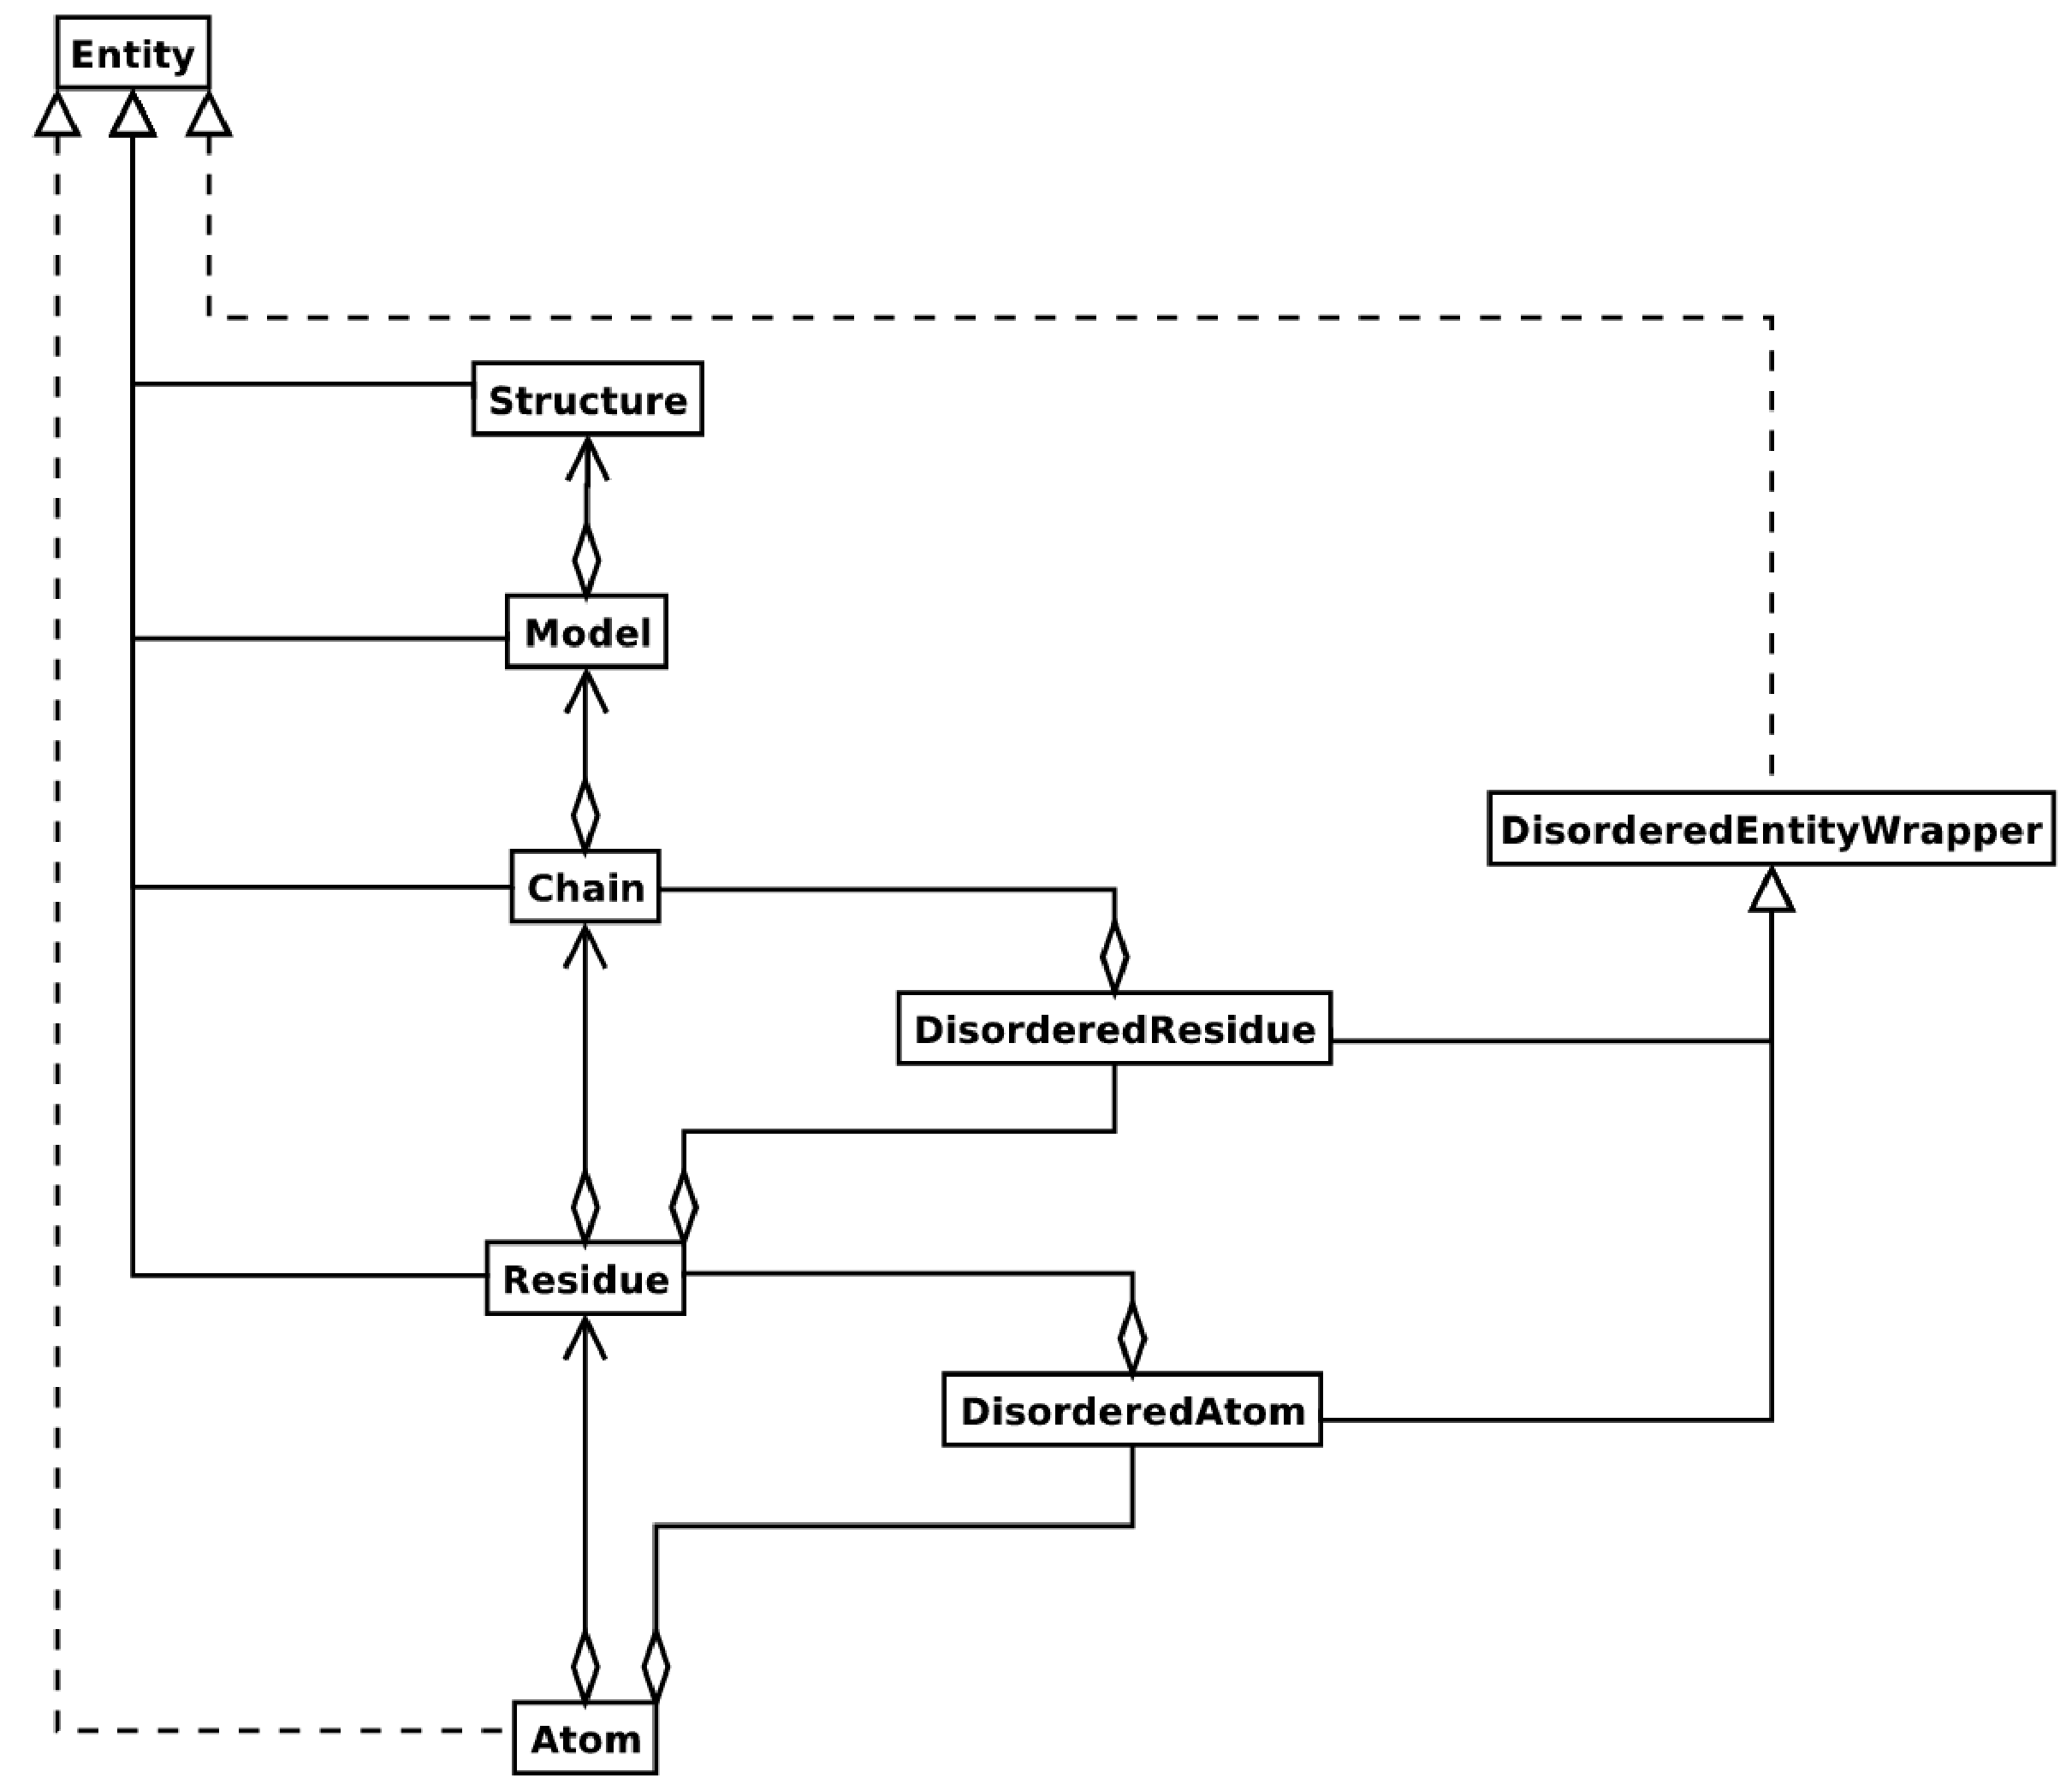
\includegraphics[width=0.8\textwidth]{images/smcra.eps}
\label{fig:smcra}
\caption{��ʬ�ҹ�¤��ɽ������ݤ˻Ȥ��� SMCRA �ǡ�����¤�� UML ���饹��}
\end{figure}

\class{Structure}��\class{Model}��\class{Chain} ����� \class{Residue}
�ϡ����������쥯�饹 \class{Entity} (����ƥ��ƥ�) �Υ��֥��饹�Ǥ���
\class{Atom} ���饹������\class{Entity} ���󥿡��ե������ΰ�������
�������Ƥ��ޤ��� (\class{Atom} ���饹�ˤϻҥ��饹��ɬ�פʤ�����Ǥ�)��

\class{Entity} ���֥��饹�Υ��֥������Ȥϡ���������դʼ��̻�
(id) �򥭡��˻Ȥ����Ȥǡ���ʬ�λҥ���ƥ��ƥ�����Ф��ޤ� (�㤨�С�
���Ҥ�̾����ɽ��ʸ����򥭡��ˤ��ơ����� \class{Residue} ���֥�������
����\class{Atom} ���֥������Ȥ���Ф����ꡤʬ�Һ��� id �򥭡���
���ơ�\class{Model} ���֥������Ȥ��� \class{Chain} ���֥������Ȥ�
���Ф�����Ǥ��ޤ�)��

���Ҥ�Ĵ�Τ�餮 (disorder) �� \class{DisorderedAtom} ��
\class{DisorderedResidue} ���饹��ɽ������ޤ��������Ϥ������
���쥯�饹\class{DisorderedEntityWrapper} �Υ��֥��饹�Ǥ���
�����Υ��饹�ϡ���餮��ȼ��ʣ�������ä��������������̤�
\class{Atom} �� \class{Residue} ���֥������ȤǤ��뤫�Τ褦�˿�����
�ޤ���

����Ū�ˤϡ�����ƥ���ƥ��ƥ� (\class{Residue}, \class{Chain},
\class{Model}, \class{Structure}) �λҤˤ����륨��ƥ��ƥ����֥�������
(\class{Atom}, \class{Residue}, \class{Model}, \class{Structure}) �ϡ�
id �򥭡��ˤ��Ƽ��Ф��ޤ���

\begin{verbatim}
child_entity=parent_entity[child_id]
\end{verbatim}

�ޤ�������ƥ���ƥ��ƥ����֥������Ȥλҥ���ƥ��ƥ����ƤΥꥹ�Ȥ�
���Ф��ޤ������Υꥹ�Ȥ��ü�ʤ�꤫�����¤�Ǥ���Τ����դ��Ƥ�����
�� (�㤨�С�\class{Model} ���֥������Ȥ��Ƥξ�硤�Ҥ�\class{Chain} 
���֥������Ȥ�¦�� id (chain identifier) �˱������¤Ӥޤ�)��

\begin{verbatim}
child_list=parent_entity.get_list()
\end{verbatim}

����ҥ���ƥ��ƥ����֥������Ȥοƥ���ƥ��ƥ����֥������Ȥ�
���Ф��ޤ���

\begin{verbatim}
parent_entity=child_entity.get_parent()
\end{verbatim}

�ޤ���SMCRA ���ؤΤɤγ��ؤΥ��֥������Ȥ��Ф��Ƥ⡤
\emph{���� id (full id)} ����Ф��ޤ���
���� id �Ȥϡ��Ǿ�̤Υ��֥������� (\class{Structure}) ���鲼�äơ�
���ߤΥ��֥������Ȥޤ�é�ä��Ȥ��˷�ͳ�������ƤΥ��֥������Ȥ� id ����
�ʤ륿�ץ�Ǥ����㤨�С����� \class{Residue} ���֥������Ȥδ��� id ��
�ʲ��Τ褦�ˤʤ�ޤ�:

\begin{verbatim}
full_id=residue.get_full_id()

print full_id

("1abc", 0, "A", ("", 10, "A"))
\end{verbatim}

���Υ��ץ�����Ƥϡ����줾��

\begin{itemize}
\item \code{"1abc"} �� id �˻��� \class{Structure} ���֥�������
\item \code{0} �� id �˻��� \class{Model} ���֥�������
\item \code{"A"} �� id �˻��� \class{Chain} ���֥�������
\item \code{("", 10, "A")} �� id �˻��� \class{Residue} ���֥�������
\end{itemize}

���б����ޤ���

�Ǹ�� \class{Residue} ���֥������Ȥ� id �ϡ��إƥ��ե������
(�ǽ�Υե������) ������ˤʤäƤ��ޤ�������ϡ����λĴ�
�إƥ��Ĵ� (�⤷���Ͽ�) �ǤϤʤ����Ȥ򼨤��Ƥ��ޤ����ޤ���
����μ��̻Ҥ� 10 �ǡ����������� (insertion code) �� \code{"A"} 
�ˤʤäƤ��ޤ���

����ƥ��ƥ��ˤϤ����Ĥ������ʥ᥽�åɤ�����ޤ�:

\begin{verbatim}
# ����ƥ��ƥ��� id ������

entity.get_id()

# ���� id ���ä��ҥ���ƥ��ƥ���¸�ߤ��뤫��Ĵ�٤�

entity.has_id(entity_id)

# �ҥ���ƥ��ƥ��ο�������

nr_children=len(entity)
\end{verbatim}

����ƥ���ƥ��ƥ����Ф��ơ����λҥ���ƥ��ƥ����������ꡤ
�ҥ���ƥ��ƥ���̾�����ѹ������ꡤ�����ʻҥ���ƥ��ƥ����ɲä������
�Ǥ��ޤ��������κݤ˥ǡ����������������å� (sanity check) ��
�Ԥ��ޤ��� (�㤨�С�����ʬ�Һ���Ʊ�� id �������ĤλĴ��
�ղä�����Ǥ��Ƥ��ޤ��ޤ�)��\class{Decorator} ���饹���Ѥ���ȡ�
��������ޤ᤿�������������å��򤦤ޤ��ԤäƤ���ޤ������⤷
�ǤΥ��󥿥ե����������Ѥ������ʤ顤������������ (\file{Entity.py})
�򻲾Ȥ��ƤߤƤ���������

\subsubsection{Structure ���֥�������}

\class{Structure} ���֥������ȤϹ�ʬ�Ҥ�ɽ������ǡ����γ��ع�¤��
ĺ���˰��֤��Ƥ��ޤ���\class{Structure} �� id �ϥ桼�������ꤷ��
ʸ����ˤʤ�ޤ���\class{Structure} ���֥������Ȥˤϡ�ʣ����
\class{Model} ���֥������Ȥ��ҥ���ƥ��ƥ��Ȥ������äƤ��ޤ���
�ۤȤ�ɤ� (���ƤǤϤ���ޤ���) �뾽��¤�ˤ�ñ��Υ�ǥ뤷��
�ʤ������� NMR �Ƿ��ꤵ��빽¤�ˤϰ���Ū�ˤ����Ĥ��Υ�ǥ뤬
���äƤ��ޤ����뾽��¤�ˤ�����¿����ʬ�Ҥˤ�餮�������Ƥ�����
�ˤ⡤ʣ���Υ�ǥ뤬�Ǥ��ޤ���

\paragraph{Structure ���֥������Ȥ��ۤ���}

\class{Structure} ���֥������Ȥ� \class{PDBParser} ���֥������Ȥ���
��������ޤ�:

\begin{verbatim}
from Bio.PDB.PDBParser import PDBParser

p=PDBParser(PERMISSIVE=1)

structure_id="1fat"

filename="pdb1fat.ent"

s=p.get_structure(structure_id, filename)
\end{verbatim}

\var{PERMISSIVE} �ե饰�ϡ�PDB �ե�����˴ؤ���褯���뤤���Ĥ�������
(\ref{problem structures} ����) ��ѡ�����̵�뤵���ޤ� (�ȤϤ�����
����ˤ�äƤ����Ĥ��θ��Ҥ�Ĵ𤬼����뤫�⤷��ʤ��Τ����դ���
��������) �����Τ��Υե饰����ꤷ�ʤ���硤�ѡ����� PDB �ե������
��ʸ���Ϥ��Ƥ���ݤ����꤬�������\exception{PDBConstructionException}
�����Ф��ޤ���

\paragraph{�إå� (header) �ȥȥ쥤�� (trailer)}

\function{get_header} ����� \function{get_trailer} �Ȥ��ä��᥽�åɤ�
�Ѥ���ȡ�PDB �ե�������Υإå��ȥȥ쥤��� (ʸ���󤫤�ʤ�ñ��ʥꥹ��
��) \class{PDBParser} ���֥������Ȥ�����Ф��ޤ���

\subsubsection{Model ���֥�������}

\class{Model} ���֥������Ȥ� id �������ǡ�PDB �ե��������Ϥ����ݤ�
���Υ�ǥ뤬���֤��Ƥ�����꤫���ޤ�ޤ� (0 ���鼫ưŪ���ֹ��դ�
����ޤ�)��\class{Model} ���֥������Ȥˤϡ��ҥ���ƥ��ƥ���\class{Chain} 
����ʤ�ꥹ�Ȥ����äƤ��ޤ���


\paragraph{����}

\class{Structure} ���֥���������˼�����Ƥ���ǽ��
��ǥ��������ޤ���

\begin{verbatim}
first_model=structure[0]
\end{verbatim}

\subsubsection{Chain ���֥�������}

\class{Chain} ���֥������Ȥ� id �ϡ���¤�ǡ������ҥե��������
��������ʬ�Һ���ɽ����ʬ�μ��̻Ҥ���Ȥ�졤���餫��ʸ����ˤʤ�ޤ���
����\class{Model} ���֥������Ȳ��ˤ���ơ���\class{Chain} �ˤ�
�ߤ��˰�դ� id ������ޤ���\class{Chain} ���֥������Ȥˤ�
�ҥ���ƥ��ƥ���\class{Residue} ����ʤ�ꥹ�Ȥ����äƤ��ޤ���

\paragraph{����}

\class{Model} ���֥������Ȥ��顤���̻� \code{"A"} ���ä�
\class{Chain} ���֥������Ȥ�������ޤ���

\begin{verbatim}
chain_A=model["A"]
\end{verbatim}

\subsubsection{Residue ���֥�������}

�����ޤǤ�ʤ���\class{Residue} �ϰ�Ϣ��\class{Atom} ��ҥ���ƥ��ƥ�
�Ȥ��Ƶ������Ƥ��ޤ�������˲ä��ơ�\class{Residue} �ˤϻĴ��̾��
�򼨤�ʸ���� (�㤨�� \code{"ASN"}) �ȡ��Ĵ�Υ������ȼ��̻�
(X-PLOR �桼���ˤϤ褯�Τ��Ƥ��ޤ�����SMCRA �ǡ�����¤���ۤ���
�ݤˤ��Ѥ����ޤ���) �����äƤ��ޤ���

\class{Residue} ���֥������Ȥ� id �ϻ��Ĥ���ʬ: �إƥ��ե������
(hetfield)�������̻� (resseq)������������ (icode) ����ʤ�ޤ���

�إƥ��ե�����ɤ�ʸ����ǡ�\code{"W"} �Ͽ��\code{"H_"} �θ����
�Ĵ�̾��³������� (�㤨�� \code{"H_FUC"}) �Ϥ���¾�Υإƥ��Ĵ��
����ϰ���Ū�ʥ��ߥλ��ȳ˻���ɽ���ޤ���������ˡ����Ѥ�����ͳ��
\ref{hetero problems} ��Dz��⤷�Ƥ��ޤ���

�Ĵ� id ������Υե�����ɤ������̻Ҥǡ�ʬ�Һ���
�ɤξ��˻Ĵ𤬷�礷�Ƥ��뤫��ɽ���ޤ���

�軰�Υե�����ɤ�ʸ����ǡ����������ɤ�����ޤ������������ɤ�
���Ф��С�����λĴ���Ф���˾�ޤ������ֹ��դ���ˡ����¸���뤿���
�Ȥ��ޤ���Ser 80 �����ߥ塼����� (�㤨�С�Thr 80 �� Asn81 �Ĵ��
�֤� Ser �����ä����) �ξ�硤�����̻Ҥ����������ɤϤ��줾��
Thr 80 A, Ser 80 B, Asn 81 �Τ褦�ˤʤ�ޤ���������ˡ��Ȥ�ȡ�
�Ĵ���ֹ��դ���ˡ���������ι�����Ʊ���ޤޤˤʤ�ޤ���

�����Ĥ����󤲤Ƥߤޤ��礦�� ���������ɤ�����ˤʤäƤ��� Asn 10 
�λĴ� id ��\code{("", 10, "")} �Ǥ���W 10 �λĴ� id ��
\code{("W", 10, "")} �Ǥ��������̻� 10 �Υ��륳����ʬ�� (�إƥ�
�Ĵ� GLC �Ȥ���̾���ˤʤäƤ��ޤ�) �� \code{("H_GLC", 10, "")}
�Ǥ������Τ褦�ˤ���ȡ����ƤλĴ�ϰۤʤ�Ĵ� id ����ĤΤǡ�
Ʊ��ʬ�Һ��ΰ���ʬ�Ȥ��ư����ޤ���

�ۤȤ�ɤξ�硤 \member{hetflag} �� \member{icode} �ե�����ɤ϶���
���ʤ��\code{("W", 10, "")} �Τ褦�ˤʤ�ޤ������Τ褦�ʾ��ˤϡ�
�����̻Ҥϴ��� id �Υ��硼�ȥ��åȤȤ������ѤǤ��ޤ�:

\begin{verbatim}
# ���� id ���

res10=chain[("", 10, "")]

# ���硼�ȥ��åȤλ��� 

res10=chain[10]
\end{verbatim}

\class{Chain} ���֥������Ⱦ�γ� \class{Residue} ���֥������Ȥˤ�
��դ� id ���Ĥ����Ƥ��ޤ����Ĵ�Τ�餮�����̰�������ޤ���
����ˤĤ��Ƥ�\ref{point mutations} ����������ޤ���

\class{Residue} ���֥������Ȥˤϡ�¾�ˤ⤤���Ĥ��᥽�åɤ�����ޤ�:

\begin{verbatim}
r.get_resname()         # "ASN" �Τ褦�ʻĴ�̾���֤�
r.get_segid()           # "CHN1" �Τ褦�� SEGID ���֤�
\end{verbatim}

\subsubsection{Atom}

\class{Atom} �ϸ��Ҥ˴�Ϣ����ǡ����򵭲������ҥ���ƥ��ƥ�������ޤ���
���Ҥ� id �Ϥ��θ��Ҥ�̾���ˤʤ�ޤ� (�㤨�С�\code{"OG"} �� Ser �Ĵ��
¦���λ��ǤǤ�)������Ĵ���Ǥϡ��ġ��θ��Ҥ� id �ϰ�դǤʤ����
�ʤ�ޤ���\ref{disordered atoms} ��Ǥ�Ҥ٤��褦�ˡ��ǡ�����ʸ����
����ݤ˸��ҤΤ�餮������������㳰��ȯ�����ޤ���

PDB �ե�������Ǥϡ����Ҥ�̾���� 4 ʸ���Υ���饯������ʤꡤ�̾��
��Ƭ�������˶��򤬤Ĥ��Ƥ��ޤ���PDB �ե�����Ǥϡ���ñ�Τ����
���Ф��Ф��ζ���Ͻ����ޤ� (�㤨�С����ߥλ�C$\alpha$ ��
PDB �ե�������Ǥ� \code{".CA."} �ǡ��ɥåȤ������ɽ���ޤ�)��
����Ĵ����̾���ξ��� (Ʊ��̾���� id ����� \class{Atom} ���֥�������
�����������) ��������ʤ��¤ꡤ���Ҥ�̾������������ݤ˥��ڡ�����
����ޤ������ͤ�ȯ�������硤�ѡ����ϥ��ڡ�����ޤ᤿����̾��Ȥ�����
��ߤޤ������Τ褦�ʾ����ϡ��㤨�а�ĤλĴ�� \code{".CA."} ��
\code{"CA.."} �Ȥ���̾���θ��Ҥ����äƤ������ȯ�����ޤ�����
��ä��˵����뤳�ȤϤ���ޤ���

�Ĵ����¸����Ƥ��븶�ҤΥǡ����ˤϡ����Ҥ�̾�������Ҥκ�ɸ
(�⤷�����ɸ���к���)��B �ե����� (�⤷����а����� B �ե�������
ɸ���к���)�� altloc ����Ҥȶ����ޤര���ʸ���̾�����äƤ��ޤ���
�����ֹ� (element number) �丶�Ҥ��Ų٤Ȥ��ä������ޤ����Ѥ���ʤ�
���Ǥϡ� PDB �ե�������ˤϽ񤫤�Ƥ��ޤ���\class{Atom} �Υǡ�����
���Ƥ���¸����ޤ���

\class{Atom} ���֥������Ȥˤϰʲ��Τ褦�ʥ᥽�åɤ�����ޤ�: 

\begin{verbatim}
a.get_name()       # ����̾ (���ڡ����ʤ����㤨�� "CA")

a.get_id()         # id (����̾��Ʊ��)

a.get_coord()      # ���Һ�ɸ

a.get_bfactor()    # B �ե�����

a.get_occupancy()  # ���Ҥ�餮�ˤ�������ͭΨ

a.get_altloc()     # _REPLACE_���ع�¤�������ֻ���� (alternative location specifier) 

a.get_sigatm()     # ���ҥѥ�᥿��ɸ���к�

a.get_siguij()     # ������ B �ե�������ɸ���к�

a.get_anisou()     # ������ B �ե�����

a.get_fullname()   # ����̾ (���ڡ�����ޤ�, ��. ".CA.")
\end{verbatim}

���Ҥκ�ɸ�������� B �ե���������Ӥ���ɸ���к���
���ҥѥ�᥿��ɸ���к���ɽ���ˤ� Numerical Python ������
�Ѥ����Ƥ��ޤ���

\subsection{��餮 (disorder)}


\subsubsection{����Ū�ʥ��ץ�����}
\label{disorder problems}

ʬ�ҹ�¤�Τ�餮 (disorder) ��ͤ���ˤϡ���Ĥλ���������ޤ���
��Ĥϸ��ҤΤ�餮���⤦��ĤϻĴ�Τ�餮�Ǥ��������Ƥ����桹��
��餮���餯��ʣ���������ƥ��ץ��벽���ư������Ȥ��Ƥ��ޤ��ޤ���
���������⤷����ñ�����Ƥ� C$\alpha$ ���Ҥˤ錄�äƥ롼�׽�����
�Ԥ����������ʤ顤�ɤ����λĴ��¦���ˤ�餮�����äƤⵤ�ˤ�
���ޤ��󡥤��ΰ����ǡ��ǡ�����¤��Ǥϡ���餮������ɽ��
�Ǥ��ʤ���Фʤ�ʤ��Ȥ������꤬����ޤ��������ǡ����Ҥ�Ĵ��
��餮���ü�ʥ��֥������Ȥ����졤���������餮��¸�ߤ��ʤ�����
�褦�˿���碌�뤳�Ȥˤ��ޤ�����������������Ԥ�ͣ�����ˡ�ϡ�
��餮����ĸ��Ҥ�Ĵ�Υ��֥��åȤˤ��ɽ���Ǥ����ɤΥ��֥��åȤ�
���Ѥ��뤫 (�㤨�С�Ser �Ĵ𤬻Ȥ��Ƥ�����ǡ����̤�ˤ�餮��
���� OG ¦���Τɤ�������֤�) �ϡ��桼��������Ǥ��ޤ���


\subsubsection{���ҤΤ�餮}
\label{disordered atoms}

���ҤΤ�餮�ξ�硤��餮�Τ�����ʬ�θ��Ҥ��̾��\class{Atom} 
���֥������Ȥ�Ȥä�ɽ�����ޤ��������������θ��Ҥ�ʪ��Ū��Ʊ��
���Ҥ�ɽ�����Ƥ���褦�ʸ��Ҥϡ����� \class{DisorderedAtom} 
���֥������������¸���ޤ���\class{DisorderedAtom} ���֥����������
��\class{Atom} ���֥������Ȥϡ�\member{altloc} ����Ҥ�Ȥäư�դ�
����Ǥ��ޤ���
\class{DisorderedAtom} ���Ф��ƥ᥽�åɸƤӽФ���Ԥ��ȡ�
\class{DisorderedAtom} �ǽ�������ʤ���Τϸ������򤵤�Ƥ���
\class{Atom} ���֥������Ȥ�ž�����ޤ����ǥե���ȤǤϡ�
��ͭΨ (occupancy) �κǤ�⤤\class{Atom} ���֥������Ȥ����򤵤��
���ޤ����������\member{altloc} �����Ѥ���С��桼���Ϥ����줫��
\class{Atom} ���֥������Ȥ�����Ǥ��ޤ������Τ褦�ˤ��ơ�������ʣ����
���������Ȥʤ������Ҥ�餮��������ɽ���Ǥ���褦�ˤʤäƤ���ΤǤ���
�̤θ������򤹤�С����Ҥ�餮�˶�̣���ʤ���С�����ˤ鷺��蘆���
ɬ�פϤʤ��Ȥ������ȤǤ���

��餮�θ��Ҥˤϡ����줾�� \member{altloc} �Ȥ������̻Ҥ�����ޤ���
\class{DisorderedAtom} ���֥������Ȥˤ��μ��̻Ҥ���ꤹ��ȡ�
����� \member{altloc} ���̻Ҥ���ä� \class{Atom} �Ǥ��뤫�Τ褦��
����碌���ޤ�:

\begin{verbatim}
atom.disordered_select("A")        # altloc �� A �θ��Ҥ����򤹤�
print atom.get_altloc()
"A"

atom.disordered_select("B")        # altloc �� B �θ��Ҥ����򤹤�
print atom.get_altloc()
"B"
\end{verbatim}

\subsubsection{�Ĵ�Τ�餮}

\paragraph{�褯���륱����}

��äȤ�褯����Τϡ��Ĵ�˰�Ĥޤ��Ϥ���ʾ�θ��ҤΤ�餮��
���륱�����Ǥ��������ޤǤ�ʤ������Υ�������\class{DisorderedAtom} 
���֥������Ȥˤ�äƤ�餮�Τ��븶�Ҥ�ɽ����������
\class{DisorderedAtom} ���֥������Ȥ�\class{Residue} ���֥������Ȥ�
������̤�\class{Atom} ���֥������ȤΤ褦�ˤ��������в�褷�ޤ���
\class{DisorderedAtom} �ϡ���ʬ��Ŭ�Ѥ��줿�᥽�åɤΤ�����
\class{DisorderedAtom} �ǽ�������ʤ���Τ�������\class{Atom} 
���֥������� (���򤵤�Ƥ��� \class{Atom} ���֥�������) 
��ž�����뤳�Ȥǡ����������̾�θ��ҤȤޤä���Ʊ���褦�� 
(�ºݤˤϺǤ���ͭΨ�ι⤤���Ҥ�Ʊ���褦��) �����񤤤ޤ���

\paragraph{���Ѱ�}
\label{point mutations}
��餮�����Ѱ� (point mutation) ��ͳ�褹��褦���ü�ʥ�������
�㤨�����Ѱ��Τ���İʾ庮���ä��ݥ�ڥץ��ɤ��뾽��˸��Ĥ���褦��
��礬����ޤ������Τ褦����ΰ�Ĥ� PDB ��¤�� 1EN2 �Ǥ���

���������ѰۤǤϡ��Ĵ� (�㤨�� Ser 60 �� Cys 60 �Τ褦��) �ۤʤ�
�Ĵ𷿤�°����Τǡ���Τ褯������Τ褦�ˡ���Ĥ� \class{Residue}
���֥������Ȥ���ˤ�����ޤ��󡥤��Τ褦�ʥ������Ǥϡ�
��餮�Ȥʤ�ơ��λĴ��\class{Residue} ���֥������Ȥ�ɽ�����Ƥ�����
ξ���� \class{Residue} ���֥������Ȥ� \class{DisorderedResidue}
���֥������Ȥ�����Ƥ����ޤ��� 

\class{DisorderedResidue} �ϡ���ʬ��Ŭ�Ѥ��줿�᥽�åɤΤ�����
\class{DisorderedResidue} �ǽ�������ʤ���Τ򸽺����򤵤��
����\class{Residue} ���֥������� (�ǥե���ȤǤϺǸ���ɲ�
���줿\class{Residue} ���֥�������) ��ž�����뤳�Ȥǡ�
���������̾�λĴ�Τ褦�˿��񤤤ޤ���\class{DisorderedResidue} 
���֥���������γ�\class{Residue} ���֥������Ȥϡ��ơ���
�Ĵ�̾�ǰ�դ˼��̤Ǥ��ޤ��������Ǥ����С� 
\class{DisorderedResidue} ���֥���������� Ser 60 �Ĵ��
���̻Ҥ�\code{"SER"} ��Cys 60 �μ��̻Ҥ�\code{"CYS"} �Ǥ���
�桼���Ϥ��μ��� id ��ȤäƸ���ͭ���� \class{Residue} ���֥�������
������Ǥ��ޤ���

\subsection{�إƥ��Ĵ�}

\subsubsection{�إƥ��Ĵ�˴�Ϣ��������}
\label{hetero problems}

�إƥ��Ĵ�˴ؤ��Ƥ褯��������ϡ������Ĥ��Υإƥ��Ĵ����إƥ��Ĵ��Ʊ��
����������Ʊ��������̻�(����������������)��ͭ���뤳�ȤǤ��롣��
�Τ��ᡢ�Ƥإƥ��Ĵ���ȼ���id���������뤿���Ȥ���¾�Υإƥ��Ĵ�ϰ�
�ʤ���ˡ�ǰ����롣

�إƥ��Ĵ�˴ؤ��Ƥ褯��������ϡ�Ʊ��ʬ�Һ���ˤ���ʣ���Υإƥ��Ĵ�
��إƥ��Ĵ𤬡�Ʊ�������̻�(���������������) ����äƤ����
�������ȤǤ����������äơ��ƥإƥ��Ĵ�� id ���դ��������뤿��ˡ�
��䤽��¾�Υإƥ��Ĵ���̤���ˡ�ǰ����ޤ���

\class{Residue} ���֥������Ȥ� \code{(hetfield, resseq, icode)} �Ȥ���
���ץ�� id ����äƤ��뤳�Ȥ�פ��Ф��Ƥ������������ߥλ���˻���
��硤 \member{hetfield} �϶� (\code{""}) �ˤʤꡤ���إƥ��Ĵ�ξ��ˤ�
ʸ����ˤʤ�ޤ���\member{hetfield} �����ƤˤĤ��Ƥϡ��ʲ����������ޤ���

\subsubsection{��Ĵ�}

��Ĵ�� \member{hetfield} ��ʸ����� \code{"W"} �ˤʤ�ޤ������Τ��ᡤ
��ΰ���Ū��id�� \code{("W", 1, "")} �Ǥ���

\subsubsection{����¾�Υإƥ��Ĵ�}

����¾�Υإƥ��Ĵ�� \member{hetfield} ʸ����ϡ�\code{"H_"} �˻Ĵ�̾��
³������ΤǤ����㤨�С��Ĵ�̾ \code{"GLC"} �Υ��륳����ʬ�Ҥξ�硤
\member{hetfield} �� \code{"H_GLC"} �ˤʤ�ޤ����Ĵ� id �� 
\code{("H_GLC", 1, "")} �Ǥ���

\subsection{������}

PDB�ե��������Ϥ��ơ�\class{Model}��\class{Chain}�� \class{Residue}
����ӡ�\class{Atom} ���֥������Ȥ���Ф��ޤ���

\begin{verbatim}
from PDBParser import PDBParser 

parser=PDBParser()

structure=parser.get_structure("test", "1fat.pdb")
model=structure[0]
chain=model["A"]
residue=chain[1]
atom=residue["CA"]
\end{verbatim}

ʬ�Һ�����إƥ��Ĵ� (�����Ǥϰ����� resseq 10 �Υ��륳���� (GLC) 
�Ǥ���褦�ʻĴ�) ����Ф��ޤ���

\begin{verbatim}
residue_id=("H_GLC", 10, " ")
residue=chain[residue_id]
\end{verbatim}

ʬ�Һ�������ƤΥإƥ��Ĵ����Ϥ��ޤ���

\begin{verbatim}
for residue in chain.get_list():
	residue_id=residue.get_id()
	hetfield=residue_id[0]
	if hetfield[0]=="H":
		print residue_id
\end{verbatim}

B �ե������� 50 �ʾ�� CA ���Ҥκ�ɸ�����ƽ��Ϥ��ޤ���

\begin{verbatim}
for model in structure.get_list():
  for chain in model.get_list():
    for residue in chain.get_list():
      if residue.has_id("CA"):
        ca=residue["CA"]
        if ca.get_bfactor()>50.0:
          print ca.get_coord()
\end{verbatim}

��餮�Τ��븶�Ҥ�ޤ����ƤλĴ����Ϥ��ޤ���

\begin{verbatim}
for model in structure.get_list()
  for chain in model.get_list():
    for residue in chain.get_list():
      if residue.is_disordered():
        resseq=residue.get_id()[1]
        resname=residue.get_resname()
        model_id=model.get_id()
        chain_id=chain.get_id()
        print model_id, chain_id, resname, resseq
\end{verbatim}

��餮�Τ��븶�����Ƥˤ錄�äƥ롼�פ��ơ����� \member{altloc} �� 
\code{"A"} �θ��� (�������) �ˤʤ�褦���򤷤ޤ�����������Ԥ��ȡ�
SMCRA �ǡ�����¤�ε�ư�� \member{altloc} �� \code{"A"} �θ��Ҥ���
¸�ߤ��ʤ����ε�ư�ˤ��ޤ���

\begin{verbatim}
for model in structure.get_list()
  for chain in model.get_list():
    for residue in chain.get_list():
      if residue.is_disordered():
        for atom in residue.get_list():
          if atom.is_disordered():
            if atom.disordered_has_id("A"):
              atom.disordered_select("A")
\end{verbatim}

ʬ�Һ��ΰ��� 10 �����Ѱۤ����äơ� Ser �� Cys ����ʤ�Ȥ��ޤ���
ʬ�Һ��ε�ư����� 10 �λĴ� Cys �Ĵ�Ǥ�����ε�ư�ˤ��ޤ���

\begin{verbatim}
residue=chain[10]
residue.disordered_select("CYS")
\end{verbatim}

\subsection{PDB �ե�����ˤ褯��������}
\subsubsection{��}
\label{problem structures}
\class{PDBParser}/\class{Structure} ���饹�ϡ�
(�ơ� SCOP �ǰۤʤ� �����ѡ��ե��ߥ꡼��°���Ƥ���) �� 800 ��
����ѥ���¤�ǥƥ��Ȥ�Ԥ��ޤ����������ˤ��� 20 ʬ���פ���
�칽¤�������ʿ�Ѥ� 1.5 �äǤ����� 64000 ���Ҥ�ޤ��ܥ������
�祵�֥�˥å� (1FKK) �Υǡ�����¤���Ϥˤϡ� 1000 MHz �� PC ���
10 �ä�����ޤ�����

���Υƥ��Ȥ���ǡ������ޤ��Ǥʤ��ǡ�����¤���ۤǤ��ʤ��Ȥ�����ͳ��
�㳰�� 3 �����Ф���ޤ�����������Υ������ˤ����Ƥ⡤���顼�θ�����
PDB �ե�����¦�ǽ������٤�����Ǥ��������������������Ǥϡ��㳰��
���Ф����������ǡ�����¤�˽񤫤�Ƥ������Ƥ���ä�ɽ�����Ƥ��ޤ�
����Ϥ뤫�ˤޤ��Ǥ���

\paragraph{�Ĵ�ν�ʣ (duplicate residues)}

���빽¤�Ǥϡ���Ĥ�ʬ�Һ������ĤΥ��ߥλ��Ĵ�Ʊ�������̻�
(resseq 3) �� icode ����äƤ��ޤ�����Ĵ�٤��Ȥ�����
����ʬ�Һ��� Thr A3, \ldots{}, Gly A202, Leu A3, Glu A204 �Τ褦��
�ʤäƤ��ޤ�����Leu A3 ���������� A203 �ʤΤ����餫�Ǥ���
Ʊ���褦�ʾ����� 1FFK �ˤ⤢��ޤ��� (Gly B64, Met B65, Glu B65, 
Thr B67, �ĤޤꡤGlu B65 �� Glu B66 �θ���)��


\paragraph{���Ҥν�ʣ (duplicate atoms)}

ʬ�ҹ�¤ 1EJG �ϡ�ʬ�Һ� A �� 22 ���ܤλĴ� Ser/Pro �����Ѱۤ�
�ʤäƤ��ޤ�������ˡ� Ser 22 �Τ����Ĥ��θ��ҤϤ�餮����äƤ��ޤ���
�������̤ꡤSer22 ��°�������Ƥθ��Ҥˤ϶���Ǥʤ� \member{altloc}
����� (B �ޤ��� C) �����ꡤPro 22 �����Ƥθ��Ҥ� \member{altloc} A
�Ǥ��������������� N �� \member{altloc} ����������ˤʤäƤ��ޤ�����
���줬�㳰�����Ф��븶���ˤʤäƤ��ޤ������Ȥ����Τ⡤���Ѱۤ�
�����Ƥ�����Ǥϡ������λĴ�������äƤ������Ƥθ��Ҥ˶���Ǥʤ�
\member{altloc} ���Ĥ��Ƥ��ʤ���Фʤ�ʤ�����Ǥ���Ser 22 �ˤ�
���� N ���ʤ��ä��Τǡ������餯���θ��Ҥ� Ser 22 �� Pro 22 �δ֤�
��ͭ����Ƥ���Τ������Ȥ������Ȥ�狼��ޤ��������ޤ���
�ե�����ˤ�����������󵯤��Ƥ��ޤ�: ���� N �� Ser �� Pro �Ĵ��
ξ���ˤʤ��ƤϤʤ餺������Ŭ�ڤ� \member{altloc} ���̻Ҥ��Ϣ�դ���
���ʤ���Фʤ�ʤ��ΤǤ���


\subsubsection{��ư����}

���顼�Τ����Ĥ��Ϥ��ʤ�褯�����Τǡ����ä�����Ԥ��ꥹ����
�������������˴�ñ�˽����Ǥ��ޤ������Τ褦�ʾ���ʲ��˼����ޤ���

\paragraph{����� altloc ��ȼ�����Ҥ�餮}

�̾��餮�θ��Ҥ� \member{altloc} ���̻Ҥ϶���Ǥ��äƤϤʤ�ޤ���
�����������λ��ͤ˽��鷺��\member{altloc} ������Τ�ΤȤ����Ǥʤ���Τ�
�ȤäƤҤȤĤθ��ҤΤ�餮��ɽ�����Ƥ����Τ�����ޤ������Τ褦��
��餮��ɽ�������äƤ⡤��ưŪ����������ˡ�Dz�ᤵ��ޤ���

\paragraph{��»���Ƥ���ʬ�Һ�}

���ˡ�ʬ�Һ� A ��°���Ƥ��뤢��Ĵ�θ����ʬ�Һ� B ��°����Ĵ�
³��������ˤ��θ����ʬ�Һ� A ��°����Ĵ𤬽и�����褦�ʻĴ���
ʬ�ҹ�¤������äƤ����硤���ʤ��ʬ�Һ�������»���Ƥ���׾�礬
����ޤ������Τ褦�ʻĴ��󤬤��äƤ⡤�����������Ԥ��ޤ���

\subsubsection{��̿Ū�ʥ��顼}

���ˡ�PDB �ե������ۣ�椵�ʤ��˲��Ǥ��ʤ���礬����ޤ������ξ�硢
���ƿ��̤�ְ㤤�Υꥹ������������Ϥ������㳰�����Ф��ơ��桼����
PDB �ե��������������褦¥���ޤ����ʲ��ˤ��Τ褦�ʥ������򼨤��ޤ���

\paragraph{�Ĵ�ν�ʣ}

����ʬ�Һ�������ƤλĴ�ˤϰ�դ� id ������ޤ������� id �ϡ�
\begin{itemize}
\item �����̻� (resseq) 
\item ���������� (icode) 
\item \member{hetfield} ʸ���� (��� \code{"W"}������¾�Υإƥ��Ĵ��
\code{"H_"} �θ���˻Ĵ�̾��³�������)
\item ���Ѱۤξ��ˤϳƻĴ�λĴ�̾ (\class{DisorderedResidue} 
���֥�������������äƤ��� \class{Residue} ���֥������Ȥξ����
����뤿��)
\end{itemize}
�˴�Ť�����������Ƥ��ޤ���
�⤷���δ��ǰ�դ� id �������Ǥ��ʤ���С��ʤˤ��ޤ������Ȥ������Ƥ���
�Ϥ��ʤΤǡ��㳰�����Ф��ޤ���


\paragraph{���Ҥν�ʣ}

����Ĵ�������Ƥθ��Ҥˤϰ�դ� id ������ޤ������� id �ϡ�
\begin{itemize}
\item ����̾ (���ڡ����ʤ������������꤬��������ϥ��ڡ�����ޤ�)
\item \member{altloc} ����� 
\end{itemize}
�˴�Ť�����������Ƥ��ޤ���

�⤷���δ��ǰ�դ� id �������Ǥ��ʤ���С��ʤˤ��ޤ������Ȥ������Ƥ���
�Ϥ��ʤΤǡ��㳰�����Ф��ޤ���


\subsection{����¾�ε�ǽ}
�뾽��¤����Ϥ��뤿��Υġ����¾�ˤ⤤���Ĥ�����ޤ�����������
�ġ���Ǥϡ�2 �Ĥκ�ɸ���åȤ�Ť͹�碌 (SVDSuperimposer) ���ꡢ
��¤����ݥ�ڥץ��ɤ���Ф���ġ��� (Polypeptide) ���ꡢ
���������Τ�õ���� (NeighborSearch) ���ꡤ PDB �ե������񤭽Ф�
(PDBIO) ����Ǥ��ޤ���
�������ѥ�����õ���ˤ� \Cpp �ǽ񤫤줿 KD �ڥ⥸�塼���ȤäƤ��ޤ���
���Υ⥸�塼��ϤȤƤ��®��ư����ߤ�������ε�Υ��ˤ���褦�����Ƥ�
��ɸ�����Ф�õ�������®�ʼ�ˡ�����äƤ��ޤ���

\class{Polypeptide} ���֥������Ȥ�ñ�� \class{Residue} ���֥������Ȥ���
�ʤ�\class{UserList} �˲᤮�ޤ���\class{Structure} ���֥������Ȥ���
\class{Polypeptide} ���֥������ȤΥꥹ�Ȥ��ۤ���ˤϰʲ��Τ褦��
���ޤ�:

\begin{verbatim}
model_nr=1
polypeptide_list=build_peptides(structure, model_nr)

for polypeptide in polypeptide_list:
    print polypeptide
\end{verbatim}

\class{Polypeptide} ���֥������ȤϾ��ñ���\class{Model} (���ξ��Ǥ�
1 ���ܤΥ�ǥ�) ������������ޤ���

\section{����¾}

\subsection{DNA ���󤫤饿��ѥ�����ؤ�����}

 % draft
\chapter{���Ը���������}

\section{���󥯥饹}

\section{�󵢥ƥ��ȥե졼����}
\label{sec:regr-test}

Biopython �ˤϲ󵢥ƥ��ȥե졼����������ޤ������Υե졼������
��Ȥ�� Andrew Dalke �ˤ�äƽ񤫤졤���θ� Brad Chapman �ˤ�ä�
PyUnit �١����˰ܿ�����ޤ������󵢥ƥ��Ȥϡ������ɤ������������
��ǽ�ʸ¤�Х���ʤ��������Ω�äƤ��ޤ���

\subsection{�󵢥ƥ��Ȥ��}

Biopython �������⥸�塼��ˤϡ����ƥƥ��Ȥ� (�����ƥɥ�����Ȥ�!)
�Ĥ��Ƥ��ʤ���Фʤ�ޤ��󡥤����ǡ����ޡ����˿������⥸�塼��
\module{Biospam} ��񤤤��Ȥ��ޤ��礦 -- �󵢥ƥ��Ȥ�������뤿���
���ʤ���Фʤ�ʤ���Ȥ�ʲ��˼����ޤ�:

\begin{enumerate}
  \item \file{test_Biospam.py} �Ȥ���̾���Υ�����ץȤ�񤭤ޤ���
  \begin{itemize}
    \item ���Υ�����ץȤ� \file{Tests} �Ȥ���̾���Υǥ��쥯�ȥ��
����ʤ���Фʤ�ޤ���
     \item ������ץȤϥ⥸�塼��ν��פʵ�ǽ���Ƥ�ƥ��Ȥ��ʤ����
�ʤ�ޤ��� (������󡤥ƥ��ȹ��ܤ�¿�����¿���ۤ��ɤ��Ǥ���!) 
  \end{itemize}
  \item ������ץȤǥƥ����ѤΥե����뤬ɬ�פʾ��ˤϡ�
\file{Tests/Biospam} �ǥ��쥯�ȥ������Ƥ����ͤФʤ�ޤ���
  \item �ƥ��ȥץ������ν��Ϥ�񤭽Ф��Ƥ��������������Ϥ���Ƥ��뤫
�Τ���ޤ�������ˤ���Ĥ���ˡ������ޤ�:
  \begin{enumerate}
    \item Ĺ����ˡ:
    \begin{itemize}
     \item ������ץȤ�¹Ԥ��ơ����Ϥ�ե�����˽񤭽Ф��ޤ���
\UNIX �ޥ���Ǥϡ� \code{python test_Biospam.py > test_Biospam} ��
�褦�˼¹Ԥ��ޤ�������ǽ��Ϥ�\file{test_Biospam} �Ȥ����ե������
�񤭽Ф���ޤ���
     \item \file{test_Biospam} ����Ȥ�Ĵ�١��������Ƥ�������
���Ȥ�Τ���ޤ����������������Ԥ��Ƥ��ơ��Х����ʤ����Ȥ��ǧ
�����顤\file{test_Biospam} �ե�������Խ����ơ���Ƭ�ιԤ�
\code{test_Biospam} �ˤʤ�褦��­���ޤ���
     \item \file{test_Biospam} �ե������\file{Tests/output}
�ǥ��쥯�ȥ������ޤ���     
   \end{itemize}
   \item ��ñ����ˡ:
   \begin{itemize}
   \item \code{python run_tests.py -g test_Biospam.py} ��¹Ԥ��ޤ���
�󵢥ƥ��ȥե졼���������ޤ�ư��ơ����ϥե����������������
���Ϥ��ޤ���
   \item ���ϥե����� (\file{Tests/output/test_Biospam} �ΤϤ��Ǥ�)
��Ĵ�١����Ƥ����������������ٳΤ���ޤ���
   \end{itemize}
 \end{enumerate}
       
 \item \file{Tests} �ǥ��쥯�ȥ�˰ܤꡤ\code{python run_tests.py} ��
�¹Ԥ��Ʋ󵢥ƥ��Ȥ����餻�ޤ������Υ��ޥ�ɤ����ƤΥƥ��Ȥ�¹Ԥ���
���������Υƥ��Ȥ�¹Ԥ���� (�����ƥѥ�����!) �Ϥ��Ǥ���
       
  \item ����ǽ����Ǥ�! ����Υ⥸�塼���Ѥ������餷���ƥ��Ȥ�
���ޤ���������ǤȤ�!
\end{enumerate}


\section{�ѡ������߷�}

\subsection{�߷פγ���}

�ѡ����ϥ��٥�Ȼظ����߷פ˱�äƺ���Ƥ��ꡤ������� (scanner)
����ӥ��󥷥塼�� (consumer) ���֥������Ȥ���ʤ�ޤ���

������ʤϥǡ����������������Ϥ������ꡤ�������Ƥ��԰��
���Ϥ��ơ��ǡ�����˲��餫�ξ��󤬸��Ĥ��뤿�Ӥ˥��٥�Ȥ�����
���ޤ����㤨�С��ǡ�����˲��餫����ʪ̾�˴ؤ���������äƤ����硤
������ʤ���ʪ̾�����ä��Ԥ��������뤿�Ӥ� \code{organism_name} 
���٥�Ȥ��������ޤ���

���󥷥塼�ޤϡ�������ʤ������������٥�Ȥ�������ޤ���
�ʲ�����Ǥϡ����󥷥塼�ޤ� \code{organism_name} ���٥�Ȥ������ꡤ
���ߤΥ��ץꥱ��������ɬ�פʤ�����˽��äƤ������Ƥ�������ޤ���

\subsection{���٥��}

���٥�Ȥˤ���Ĥμ���: info ���٥�Ȥ� section ���٥�Ȥ�����ޤ���
info ���٥�Ȥϡ��ǡ������ȥ꡼����ξ���Τ�����򥿥��դ����ޤ���
section ���٥�Ȥϥ��ȥ꡼�������ʬ (section) ��ޡ������ޤ���
info ���٥�Ȥϥǡ����������ιԤ˴�Ϣ�Ť����ޤ��������������
���٥�ȤϤ����ǤϤ���ޤ���

��������󥤥٥��̾��ɬ�� \code{start_EVENTNAME} �����
\code{end_EVENTNAME} �Ȥ���̾���ˤ��ޤ���\code{EVENTNAME} ��
���٥�Ȥ�̾���Ǥ���

�㤨�С� FASTA �����������������Υ�����ʤǤϡ��ʲ��Τ褦�ʥ��٥��
����������ޤ�:
\begin{verbatim}
EVENT NAME      ORIGINAL INPUT
begin_sequence  
title           >gi|132871|sp|P19947|RL30_BACSU 50S RIBOSOMAL PROTEIN L30 (BL27
sequence        MAKLEITLKRSVIGRPEDQRVTVRTLGLKKTNQTVVHEDNAAIRGMINKVSHLVSVKEQ
end_sequence
begin_sequence
title           >gi|132679|sp|P19946|RL15_BACSU 50S RIBOSOMAL PROTEIN L15
sequence        MKLHELKPSEGSRKTRNRVGRGIGSGNGKTAGKGHKGQNARSGGGVRPGFEGGQMPLFQRLPK
sequence        RKEYAVVNLDKLNGFAEGTEVTPELLLETGVISKLNAGVKILGNGKLEKKLTVKANKFSASAK
sequence        GTAEVI
end_sequence
[...]
\end{verbatim}

(���ɤ���褯���뤿��˰������ä�û�����Ƥ���ޤ�)

�����Ǥϡ�FASTA ������ʤ� \code{title}��\code{sequence}��
\code{begin_sequence}��\code{end_sequence} �Ȥ������٥�Ȥ�
�������Ƥ��ޤ���\code{begin_sequence} ��\code{end_sequence} 
�������� FASTA ���ϥǡ����Τ�����ιԤȤ��Ϣ�դ����Ƥ��ʤ�
���Ȥ����դ��Ƥ������������Υ��٥�Ȥϡ��ե���������̡�������
�������ڤ뤿��˻Ȥ��Ƥ��ޤ���

������ʤ������Ǥ��륤�٥�Ȥϡ����줾��Υǡ����������Ȥ�
��ޤäƤ��ޤ���

\subsection{'noevent' EVENT}

�ǡ����ե�������ˤϡ����ԤΤ褦��������̣�Τʤ��������äƤ���
���Ȥ⤢��ޤ����ص��塤������ʤϤ�������̵��̣�ʹԤ��Ф��Ƥ�
\code{"noevent"} �Ȥ������٥�Ȥ��������ʤ���Фʤ�ޤ���

\subsection{�������}

\begin{verbatim}
class Scanner:
    def feed(self, handle, consumer):
        # ������ʬ
\end{verbatim}

������ʤϡ��ե�����ϥ�ɥ�ȥ��󥷥塼�ޤ�����ˤȤ�
\function{feed} �Ȥ���̾���Υ᥽�åɤ�������Ƥ��ʤ���Фʤ�ޤ���
������ʤϥե�����ϥ�ɥ뤫��ǡ������ɤ߽Ф������󥷥塼�ޤ��Ф���
Ŭ�ڤʥ��٥�Ȥ����Ф��ͤФʤ�ޤ���

\subsection{���󥷥塼��}

\begin{verbatim}
class Consumer:
    # ���٥�ȥϥ�ɥ�
\end{verbatim}

���󥷥塼�ޤˤϡ����٥�Ȥ�������뤿��Υ᥽�åɤ�����Ƥ����ޤ���
�᥽�åɤ�̾���ϡ����󥷥塼�ޤ��������륤�٥�Ȥ�̾���ˤʤ�ޤ���
info ���٥�Ȥξ��ˤϡ����٥�Ȥ˴�Ϣ������������ä��ǡ����Ԥ�
�Ϥ���ޤ��� section ���٥�Ȥξ��ˤϲ����Ϥ���ޤ���

��ʬ�Υ��ץꥱ�������Ȥϴط��ʤ����٥�Ȥ�̵�뤷�Ƥ��ޤ��ޤ���
�����������٥�ȤΥ᥽�åɤϼ������ʤ��Ǥ����ޤ���

���󥷥塼�ޤϡ�\class{Consumer} ���饹����Ƴ�Ф��ʤ���Фʤ�ޤ���

�ʲ�����򼨤��ޤ�:

\begin{verbatim}
class FASTAConsumer(Consumer):
    def title(self, line):
        # �����ȥ�Ԥ��������
    def sequence(self, line):
        # �������γƹԤ��������
    def begin_sequence(self):
        # �������γ�����ʬ
    def end_sequence(self):
        # �������ν�λ��ʬ
\end{verbatim}


\subsection{BLAST}

BLAST ������ʤϰʲ��Τ褦�ʥ��٥�Ȥ��������ޤ�:

\begin{verbatim}
header
    version
    reference
    query_info
    database_info

descriptions
    description_header
    round                         psi blast
    model_sequences               psi blast
    nonmodel_sequences            psi blast
    converged                     psi blast
    description
    no_hits

alignment
    multalign                     master-slave
    title                         pairwise
    length                        pairwise
  hsp
    score                         pairwise
    identities                    pairwise
    strand                        pairwise, blastn
    frame                         pairwise, blastx, tblastn, tblastx
    query                         pairwise
    align                         pairwise
    sbjct                         pairwise

database_report
    database
    posted_date
    num_letters_in_database
    num_sequences_in_database
    num_letters_searched          RESERVED.  ���߻Ȥ��Ƥ��ʤ��Ϥ���
    num_sequences_searched        RESERVED.  blastool.c �ˤϤ��뤬...
    ka_params
    gapped                        not blastp
    ka_params_gap                 gapped mode (not tblastx)

parameters
    matrix
    gap_penalties                 gapped mode (not tblastx)
    num_hits                      
    num_sequences                 
    num_extends                   
    num_good_extends              
    num_seqs_better_e
    hsps_no_gap                   gapped (not tblastx) and not blastn
    hsps_prelim_gapped            gapped (not tblastx) and not blastn
    hsps_prelim_gap_attempted     gapped (not tblastx) and not blastn
    hsps_gapped                   gapped (not tblastx) and not blastn
    query_length
    database_length
    effective_hsp_length
    effective_query_length
    effective_database_length
    effective_search_space
    effective_search_space_used
    frameshift                    blastx or tblastn or tblastx
    threshold
    window_size
    dropoff_1st_pass
    gap_x_dropoff
    gap_x_dropoff_final           gapped (not tblastx) and not blastn
    gap_trigger
    blast_cutoff
\end{verbatim}

\subsection{Enzyme}
Enzyme ������ʤϰʲ��Υ��٥�Ȥ��������ޤ�:
\begin{verbatim}
record
    identification
    description
    alternate_name
    catalytic_activity
    cofactor
    comment
    disease
    prosite_reference
    databank_reference
    terminator
\end{verbatim}

\subsection{Fasta}
Fasta ������ʤϰʲ��Υ��٥�Ȥ��������ޤ�:
\begin{verbatim}
sequence
    title
    sequence
\end{verbatim}


\subsection{Medline}
MEDLINE �η����ϡ�\ulink{Online Service Reference Manual}{http://www.nlm.nih.gov/pubs/osrm_nlm.html}
�˥ɥ�����Ȳ�����Ƥ��ޤ���

Medline ������ʤϰʲ��Τ褦�ʥ��٥�Ȥ��������ޤ�:
\begin{verbatim}
record
    undefined
    abstract_author
    abstract
    address
    author
    call_number
    comments
    class_update_date
    country
    entry_date
    publication_date
    english_abstract
    entry_month
    gene_symbol
    identification
    issue_part_supplement
    issn
    journal_title_code
    language
    special_list
    last_revision_date
    mesh_heading
    mesh_tree_number
    major_revision_date
    no_author
    substance_name
    pagination
    personal_name_as_subject
    publication_type
    number_of_references
    cas_registry_number
    record_originator
    journal_subset
    subheadings
    secondary_source_id
    source
    title_abbreviation
    title
    transliterated_title
    unique_identifier
    volume_issue
    year
    pubmed_id
\end{verbatim}    

\code{undefined} �ϡ����ͤˤʤ������ (qualifier) �ΤĤ����Ԥ�
�������뤿�Ӥ����Ф�����ü�ʥ��٥�ȤǤ���

\subsection{Prosite}
Prosite ������ʤϰʲ��Τ褦�ʥ��٥�Ȥ��������ޤ�:
\begin{verbatim}
copyrights
    copyright
record
    identification
    accession
    date
    description
    pattern
    matrix
    rule
    numerical_results
    comment
    database_reference
    pdb_reference
    documentation
    terminator
\end{verbatim}

PRODOC ������ʤϰʲ��Τ褦�ʥ��٥�Ȥ��������ޤ�:
\begin{verbatim}
record
    accession
    prosite_reference
    text
    reference
\end{verbatim}


\subsection{SWISS-PROT}
SProt ������ʤϰʲ��Τ褦�ʥ��٥�Ȥ��������ޤ�:
\begin{verbatim}
record
    identification
    accession
    date
    description
    gene_name
    organism_species
    organelle
    organism_classification
    reference_number
    reference_position
    reference_comment
    reference_cross_reference
    reference_author
    reference_title
    reference_location
    comment
    database_cross_reference
    keyword
    feature_table
    sequence_header
    sequence_data
    terminator
\end{verbatim}

KeyWList ������ʤϰʲ��Τ褦�ʥ��٥�Ȥ��������ޤ�:
\begin{verbatim}
header
keywords
    keyword
footer
    copyright
\end{verbatim}

\section{�ִ�����}

\subsection{SubsMat �⥸�塼��}

���Υ⥸�塼��Ǥϡ�BLOSUM �� PAM �Τ褦���ִ�������������뤿���
���饹�Ȥ����Ĥ��Υ롼������󶡤��Ƥ��ޤ������������ִ������
�桼�����󶡤����ǡ������������Ǥ���褦�ˤʤäƤ��ޤ���

�ä��ơ����Ǥ��󾧤���Ƥ����ִ�����򥳥쥯����󤷤Ƥ���
\file{MatrixInfo.py} �����ִ���������٤�褦�ˤ�ʤäƤ��ޤ���

\begin{classdesc}{SeqMat}{data=None, alphabet=None, 
    mat_type=NOTYPE, mat_name='', build_later=0}

\class{UserDict.UserDict} �Υ��֥��饹�Ǥ���
\var{data} �ϼ���ޤ���¾�� \class{SeqMat} ���󥹥��󥹤ˤǤ��ޤ���
\var{alphabet} �� \class{Bio.Alphabet} �Υ��󥹥��󥹤Ǥ���
\var{alphabet} ����Ϥ���ȡ�\var{data} ���饢��ե��٥åȤ���
���ޤ���
\var{mat_type} �ˤ�������������Υ����פ���ꤷ�ޤ�:
      \begin{description}
        \item[NOTYPE]     ����ʤ�
        \item[ACCREP]     �����ִ����� (Accepted Replacements Matrix)
        \item[OBSFREQ]    ��¬���ٹ��� (Observed Frequency Matrix)
        \item[EXPFREQ]    ���ٴ����͹��� (Expsected Frequency Matrix)
        \item[SUBS]       �ִ����� (Substitution Matrix)
        \item[LO]         �п���Ψ���� (Log Odds Matrix)
      \end{description}

\var{mat_type} ��\class{SubsMat} �δؿ���ƤӽФ��ݤ˼�ưŪ�˷��ꤵ��ޤ���
\var{mat_name} �� \code{"BLOSUM62"} �� \code{"PAM250"} �Τ褦��
�����̾���Ǥ���
\var{build_later} �ϥǥե���Ȥ�\constant{False} �Ǥ���
\constant{True} �ˤ�����硤��ǹ����������뤿��ˡ��桼����
����ե��٥åȤȶ��μ�����������Ǥ��ޤ������ΤȤ�������ե��٥åȤ�
�������ȹ���Υ������δ֤��������Υ����å���Ԥ��ޤ���
\end{classdesc}

\subsubsection{°��}

\begin{memberdesc}{data}
\var{data} �ϼ���ǡ�
    \code{\{(i1,j1):n1, (i1,j2):n2,...,(ik,jk):nk\}} �Τ褦�ʷ�����
�Ȥ�ޤ���\code{i} ����� \code{j} �ϥ���ե��٥å�ʸ���ǡ�\code{n}
��\code{i} ��\code{j} ���ִ����Ф����ͤǤ���
\end{memberdesc}

\begin{memberdesc}{alphabet}
\var{alphabet} ��\class{Bio.Alphabet} ���������Ƥ��륢��ե��٥å�
�Ǥ���
\end{memberdesc}

\begin{memberdesc}{ab_list}
����ե��٥åȤ�ʸ���ꥹ�Ȥ򥽡��Ȥ�����ΤǤ�������������Ѹ�����
°���Ǥ���
\end{memberdesc}

\begin{memberdesc}{sum_letters}
����ǡ� \code{\{i1: s1, i2: s2,...,in:sn\}} �Τ褦�ʷ�����Ȥ�ޤ���
\code{i}, \code{s}, \code{n} �Ϥ��줾��:
    \begin{enumerate}
      \item i: ����ե��٥å����ʸ����
      \item s: ����ʸ�����Ф���Ⱦ����������Ƥ��ͤ��פ�����Ρ�
      \item n: ����ե��٥å����ʸ������
    \end{enumerate}
�Ǥ���
\end{memberdesc}

\subsubsection{�᥽�å�}

\begin{methoddesc}{entropy}{obs_freq_mat}
��¬���ٹ��� (observed frequency matrix) 
\var{obs_freq_mat} ������٤˴�Ť��ơ�����Υ���ȥ��ԡ���
�֤��ޤ������󥤥󥹥��󥹤� \code{LO} �ޤ��� \code{SUBS} ��
�ʤ���Фʤ�ޤ���
\end{methoddesc}

\begin{methoddesc}{letter_sum}{letter}
\var{letter} ���б��������������Ƥ��ͤ�û������֤��ޤ���
\end{methoddesc}

\begin{methoddesc}{all_letter_sum}{}
\member{sum_letters} °�����ͤ򡤹���Υ���ե��٥åȤγ�ʸ����
�Ф����ͤι�פ����ޤ���
\end{methoddesc}

\begin{methoddesc}{print_mat}{f, format="%4d", bottomformat="%4s",
    alphabet=None}
�����ե�����ϥ�ɥ� \var{f} �˽��Ϥ��ޤ���\var{format} ��
����γ��ͤ���Ϥ���ݤ˻Ȥ��񼰲�ʸ����Ǥ���
\var{bottomformat} �ϺDz��ʤγƥե�����ɤ�񼰲�����ݤ˻Ȥ�
ʸ����ǡ��ƥե�����ɤϹ������ʸ����ޤ�褦�ˤʤäƤ��ޤ���
��ʸ���Υ���ե��٥åȤ���ʤ����ν�����򲼤˼����ޤ�:

\begin{verbatim}
A 23
B 12 34
C 7  22  27
  A   B   C
\end{verbatim}

���ץ����ΰ���\var{alphabet} �ϡ�����ե��٥å����Ƥ�
���ä�ʸ����Ǥ���\var{alphabet} ����ꤷ����硤
���˻Ȥ��륢��ե��٥åȤν��֤ϡ�����ե��٥åȽ�ǤϤʤ�
ʸ������ν��֤ˤʤ�ޤ���
\end{methoddesc}



\subsection{����ˡ}

�ʹߤ���ϡ��п���Ψ���������������͸����˹�������Ƥ��ޤ���
����������Ū�ʾ����ɽ�����������������Ĵ�٤����Ǥ��ޤ�����
�ۤȤ�ɤοͤ��п���Ψ����������������ʤΤǡ������ǤϤ��������
�����ޤ���
   
\subsubsection{�����ִ����������}

�ǽ�ˡ��ǡ�����������ִ����� (Accepted Replacement Matrix, ARM) ��
��������ɬ�פ�����ޤ���ARM ����ͤϡ��ǡ�����λĴ��ִ��������
��ΤǤ������äơ����Ȥ��Х���˥󤫤饷���ƥ���ؤ��ִ��� 10 ��
�����Ƥ��ꡤ�����ƥ��󤫤饢��˥�ؤ��ִ��� 12 �󵯤��Ƥ���С�
ARM �ϰʲ��Τ褦�ˤʤ�ޤ�:

\begin{verbatim}
('A','C'): 10, ('C','A'): 12 
\end{verbatim}

�Ĵ�֤ν���϶��̤��ʤ��Τǡ��ºݤˤϥ���ȥ���Ļ��ꤹ�������
��ʬ�Ǥ�:

\begin{verbatim}
('A','C'): 22 
\end{verbatim}

\class{SeqMat} ���󥹥��󥹤ϡ������� (���Ԥ���ˡ: 10, 12) �ˤ�
Ⱦ���� (��Ԥ���ˡ: 22) �ˤ������Ǥ��ޤ���
����ѥ����󥢥�ե��٥åȤ��Ф���������Υ������� 20x20 = 400 
�ˤʤ�ޤ���Ⱦ����ξ��� 20x20/2 + 20/2 = 210 �Ǥ���
����ϡ�Ʊ��ʸ��Ʊ�Τ��Ȥ߹�碌����ʤ륨��ȥ� (������г���ʬ��
�ʤ�ޤ�) ���Ѳ����ʤ�����Ǥ������ʤ����
����ե��٥åȤο��� N �Ȥ���ȡ�

   \begin{enumerate}
     \item ������:N*N 

     \item Ⱦ����: N(N+1)/2 
   \end{enumerate}

�ˤʤ�ޤ���

\class{SeqMat} �Υ��󥹥ȥ饯������������Ϥ��ȡ���ưŪ��
Ⱦ������������ޤ���Ⱦ������Ϥ����ˤϡ������Ȥʤ�Ĵ��ִ�
���Ȥ߹�碌�ϥ���ե��٥åȽ�ˤ��Ƥ����ͤФʤ�ޤ���: �Ĥޤꡤ
\code{('A', 'C')} �Ϥ��ޤ��ޤ��󤬡�\code{('C', 'A')} �Ȥ��Ƥ�
�ʤ�ޤ���

��Ū���п���Ψ��������������ʤ顤���λ�����\ref{sec:LOMsample} ��
�˿ʤ�Ǥ����������ʹߤΥƥ����ȤǤϡ��˻��䥢�ߥλ������پ����
������Ū��Ĵ�٤����͸����ˡ��п���Ψ�����������������������
����Ƥ���ؿ��ˤĤ����������Ƥ��ޤ���

\subsubsection{��¬�ٿ����� (Observed Frequency Matrix:OFM) ������}

\begin{funcdesc}{_build_obs_freq_mat}{ARM}
OFM �� ARM �����������ޤ���ARM �Ȥΰ㤤�ϡ��ִ�����ǤϤʤ�
�ִ����٤����äƤ���Ȥ������Ȥ����Ǥ���
\end{funcdesc}

\subsubsection{�����ٿ����� (Expected Frequency Matrix:EFM) ������}

\begin{funcdesc}{_build_exp_freq_mat}{OFM, exp_freq_table}

\var{exp_freq_table} �ϡ�\class{FreqTable} �Υ��󥹥��󥹤�
�ʤ��ƤϤʤ�ޤ���\class{FreqTable} �ξܺ٤� \ref{sec:freq-table}
��򻲾Ȥ��Ƥ�������������Ǹ����ȡ������ٿ�����ˤϡ�
����ե��٥å���γ�ʸ�������٤����äƤ��ޤ���EFM �ϥ���ե��٥å����
��ʸ���򥭡��Ȥ��뼭��ˤʤäƤ��ơ����٤��ͤȤ����б����Ƥ��ޤ���
���٤ι�פ� 1 �ˤʤ�ޤ���
\end{funcdesc}
 
�����ٿ�ɽ�ϡ���¬�ٿ����󤫤������Ǥ��ޤ� (�̾�Ϥ������ޤ�)��
���äơ��ۤȤ�ɤξ��ˤϡ��ʲ��Τ褦�ˤ���\var{exp_freq_table} 
���������ޤ�:

\begin{verbatim}
>>> exp_freq_table = SubsMat._exp_freq_table_from_obs_freq(OFM)
>>> EFM = SubsMat._build_exp_freq_mat(OFM,exp_freq_table)
\end{verbatim}

�ȤϤ���������� \var{exp_freq_table} �����ϤǤ��ޤ���

\subsubsection{�ִ����ٹ��� (Substitution Frequency Matrix:SFM) ������}

\begin{funcdesc}{_build_subs_mat}{OFM, EFM}

\var{OFM} ����� \var{EFM} �������ꡤ�б������ʹ֤ǽ�����Ԥä�
��̤��֤��ޤ���
\end{funcdesc}

\subsubsection{�п���Ψ���� (Log Odds Matrix:LOM) ������}

\begin{funcdesc}{_build_log_odds_mat}{SFM, logbase=10,factor=10.0,
    round_digit=1}

\var{SFM} ������˼������ޤ� \var{logbase} ���п���Ψ�����
��������ݤ˻Ȥ��п�����Ǥ���\var{factor} �ϡ��п���Ψ�����
�����Τ˾軻������ͤǤ�������γ��ͤϡ�\code{log(LOM[key])*factor} 
�ˤʤ�ޤ��������� \var{round_digit} ���ɬ�פ˱������ͤ�ݤ�ޤ���
\end{funcdesc}

\subsubsection{����}
\label{sec:LOMsample}

�ۤȤ�ɤοͤϤǤ��������ȴ���򤷤��п���Ψ�����������������
�פäƤ���Ǥ��礦���顤\class{SubsMat} �Ǥ����Ƥκ�Ȥ�
��Ĥδؿ��ǹԤ���褦�ˤ��Ƥ��ޤ�:

\begin{funcdesc}{make_log_odds_matrix}{acc_rep_mat,
    exp_freq_table=None, logbase=10, factor=10.0, round_digit=0}

\var{acc_rep_mat} �ϼ����ִ�����Ǥ���\var{exp_freq_table} ��
�����٥ơ��֥�ǡ����ꤷ�ʤ����\var{acc_rep_mat} �����������ޤ���
\var{logbase} ���п���Ψ������п�����ǡ��ǥե���Ȥ��ͤ� 10 �Ǥ���
\var{round_digit} �Ͼ����ʲ��Ǥδݤ����ǡ��ǥե���Ȥ��ͤϥ����Ǥ���
\end{funcdesc}


\subsection{FreqTable}
\label{sec:freq-table}

\begin{classdesc}{FreqTable}{}
\end{classdesc}

\subsubsection{°��}


\begin{memberdesc}{alphabet}
\class{Bio.Alphabet} �Υ��󥹥��󥹤Ǥ���
\end{memberdesc}

\begin{memberdesc}{data}
���ټ���Ǥ���
\end{memberdesc}

\begin{memberdesc}{count}
(������Ȥ�Ϳ�����Ƥ������) ������ȼ���Ǥ���
\end{memberdesc}

\subsubsection{�᥽�å�}

\begin{methoddesc}{read_count}{f}
���ȥ꡼��\var{f} ���饫����ȥե�������ɤ߽Ф������٤��Ѵ����ޤ���
\end{methoddesc}

\begin{methoddesc}{read_freq}{f}
���ȥ꡼��\var{f} �������٥ǡ������ɤ߽Ф��ޤ������ξ�硤������
������Ȥ������ޤ��󤬡��̾��ʸ�����٤�����ɬ�פǤ���
\end{methoddesc}

\subsubsection{������}

�ǡ����١�����λĴ�������ʲ��Τ褦�ʶ�����ڤ�η����ǥե������
���äƤ���Ȥ��ޤ� (������Ǥ� 3 �ĤΥ���ե��٥åȤ������äƤ��ޤ�):

\begin{verbatim}
A   35
B   65
C   100
\end{verbatim}

�ǡ������ɤ߹��ߤ� \code{FreqTable.read_count(file_handle)}
�ǹԤ��ޤ���

Ʊ�����Ƥδ����ٿ��ե�����ϰʲ��Τ褦�ˤʤ�ޤ�:

\begin{verbatim}
A  0.175
B  0.325
C  0.5 
\end{verbatim}

�������Ĵ�����٤���ϼ���Ǥ��Ϥ��ޤ���
(3 ʸ������ե��٥åȤξ���) �Ĵ������ϰʲ��Τ褦�ˤʤ�ޤ�:

\begin{verbatim}
{'A': 35, 'B': 65, 'C': 100}
\end{verbatim}

���λĴ���ǡ������顤\code{'C'} �����٤� 0.5 ��\code{'B'} ��
0.325��\code{'A'} �� 0.175 �ǡ������ A, B, C �ι���� 200 
�ˤʤ�ޤ���

Ʊ���ǡ��������ټ����ɽ���Ȱʲ��Τ褦�ˤʤ�ޤ�:

\begin{verbatim}
{'A': 0.175, 'B': 0.325, 'C': 0.5}
\end{verbatim}

��פ� 1 �ˤʤäƤ��ޤ��͡�

���񷿤�������Ϥ���硤�Ĵ���μ���ʤΤ����٤μ���ʤΤ���
���ꤻ�ͤФʤ�ޤ��󡥤��Τ��ᡤ\class{FreqTable} ���饹��
���󥹥ȥ饯���ˤ���Ĥΰ����������Τȡ���������Ƥ�ɽ��
����ܥ����ꤹ��ɬ�פ�����ޤ�������ܥ��
\constant{FreqTable.COUNT} �ޤ���\constant{FreqTable.FREQ}
�ǡ����줾��Ĵ�������٤򼨤��ޤ���

�ʲ��Τɤ��ȤäƤ⡤���٥ơ��֥� (ftab) ������Ǥ��ޤ�:

\begin{verbatim}
>>> from SubsMat import *
>>> ftab = FreqTable.FreqTable(my_frequency_dictionary,FreqTable.FREQ)
>>> ftab = FreqTable.FreqTable(my_count_dictionary,FreqTable.COUNT)
>>> ftab = FreqTable.read_count(open('myCountFile'))
>>> ftab = FreqTable.read_frequency(open('myFrequencyFile'))
\end{verbatim}




\chapter{���ϲ��� -- Biopython �ץ��������Ȥؤι׸�}

\section{����ץ�åȥե������������ʪ�Υ��ƥʥ�}
\label{sec:maintain-dist}

Biopython �κ�Ԥ����ϡ��桼���Υ��󥹥ȡ����Ȥ��Ǥ��������ñ��
�ʤ�褦�˥�꡼����������褦�����Ϥ��Ƥ��ޤ������Τ��ᡤBiopython
�Υ饤�֥����󶡤Ǥ���¤������Υ��󥹥ȡ�����������ۤ��Ƥ��ޤ���
��꡼���򹹿����뤿�Ӥ����ƤΥ��󥹥ȡ����������������Ȥ�
��ȯ�ԤˤȤä�����ˤʤꡤ���ޤ�ܤ����ʤ��褦�ʷ����Υѥå�������
���ƥʥ󥹤���ɬ�פ������뤳�Ȥ�����ޤ���
����Ǥϡ���ȯ�԰ʳ��ο͡��˳ƥץ�åȥե���������Υӥ�ɤ�
���ƥʥ󥹤��Ƥ�館��褦�ˡ������Ĥ���Ʀ�μ����󶡤��褦��
�ͤ��Ƥ��ޤ���

�绨�Ĥ˸����С��ƥץ�åȥե���������ӥ�ɤΥ��ƥʥ󥹺�Ȥ�
���ʤ��ñ�Ǥ� -- ���ͤФʤ�ʤ����Ȥϡ������꡼��������
����뤿�Ӥˡ�����Υ����ƥ�����Υѥå����������������Ȥ����Ǥ���
������󡤤��θ�ѥå�����������å����ơ����󥹥ȡ��뤬���ޤ�������
�Τ����ɬ�פϤ���ޤ����������줿�ѥå���������פʳ�ȯ�����åդ�ï����
����С���餬 Web �����Ȥ˥ѥå������ؤΥ�󥯤�Ž���դ��Ƥ���ޤ���
��������� Biopython �˹׸��������Ȥˤʤ�ޤ��������餷����

�ƥץ�åȥե���������ˡ����ƺ�Ȥ�ԤäƤߤ褦�ȹͤ��Ƥ���ͤ�
������ˤʤ�褦�ʾ����ʲ��˼����ޤ�:

\subsection{RPM ��}

RPM �Ϥ����Ĥ��Υץ�åȥե���������Ѥ���Ƥ��뤫�ʤ�ͭ̾��
�ѥå��������������ƥ�Ǥ���RPM �ˤĤ��Ƥβ�����������ꡤ
\url{http://www.rpm.org} ��������Ǥ��ޤ�������ץ�åȥե�����
������ RPM �κ��������˴�ñ�Ǥ���ɬ�פʤΤϡ�ñ�˥����������ɤ���
�ӥ�ɤ�Ԥ��� (������󡤤������ư��륳��ѥ������äƤ��뤳��
��ɬ�ܾ��Ǥ�) �Ȥ������Ȥ����Ǥ����ܤ����� Biopython ���󥹥ȡ���
������ (Biopython installation instructions) �򻲾Ȥ��Ƥ���������

�̾ RPM �κ����ϡ��ʲ��Υ��ޥ�ɤ�¹Ԥ�������ǤǤ��ޤ�:

\begin{verbatim}
python setup.py bdist_rpm
\end{verbatim}

���Υ��ޥ�ɤǡ����߻ȤäƤ���ץ�åȥե���������� RPM ��
\file{dist} �ǥ��쥯�ȥ�β��˺�������ޤ����������줿 RPM ������ʤ�
���ѤǤ���С���ȤϽ����Ǥ�����ñ�Ǥ��͡�


\subsection{Windows ��}

Windows �Ǥˤ��̾�褯�Ǥ��� GUI �١����Υ��󥹥ȡ��餬�Ĥ�����ơ�
ɬ�פʥ���ݡ��ͥ�Ȥ����������˥��󥹥ȡ��뤷�Ƥ���ޤ���
���μ�Υ��󥹥ȡ���ϡ�\module{Distutils} ��ȤäƤ��ʤ��ñ��
�����Ǥ��ޤ���

�ޤ�����ʬ�� Windows ����ԥ塼����ư����C ����ѥ������äƤ��ꡤ
���Υ���ѥ���� Biopython �򥳥�ѥ��뤷�ƥ��󥹥ȡ���Ǥ��ͤ�
�ʤ�ޤ���(������� Biopython ���󥹥ȡ��륬���ɤ򻲾Ȥ��Ƥ�������)��

C ����ѥ�������ꤷ�Ƥ���С����󥹥ȡ���κ����ϰʲ��Τ褦��
��������Ǥ�:

\begin{verbatim}
python setup.py bdist_wininst
\end{verbatim}

����� Windows �ǥ��󥹥ȡ��餬�������ޤ�������ǤȤ�!

\subsection{Macintosh ��}

�����ϡ� Macintosh �Ǥ�����ʪ����ƥʥ󥹤��ơ� bin-hex ��
�褦�� Macintosh �ե��ɥ�ʷ��������ѤǤ���褦�ˤ��Ƥ����ͤ�
����Ƥ���ʤ�����Ǯ˾���Ƥ��ޤ���
����Ū�ˤϡ� Mac ������Ƥ򥳥�ѥ��뤹����ˡ�򸫤Ĥ����ꡤ
UNIX �١����γ�ȯ�Ԥ��񤤤����������Ƥ� Mac �Ǥ�������ư��뤳�Ȥ�
��ǧ�����ꡤMac �ե��ɥ�ʥҥ�Ȥ򶵤��Ƥ����ͤ�ɬ�פǤ���

�⤷���ʤ��� Mac �桼���ǡ�Biopython �Υѥå�����������Ǥ����顤
��ʬ�Υ����ƥ�ǥƥ��Ȥ��ơ����󥹥ȡ��뤬���Ƥ��ޤ�������������
ư���Ƥ���������ǧ���Ƥ������������ޤ��ԤäƤ���� Biopython 
��ȯ�Ԥ�ï�������äƤ������� (ï������Ф褤���狼��ʤ���С�
Biopytho@Biopython.org �Υ᡼��󥰥ꥹ�Ȥ����äƤ�������)
����Ǵ�λ�Ǥ������꤬�Ȥ���


\section{�Х����䵡ǽ�ɲä���˾}

Biopython �⥸�塼����Ф���ե����ɥХå��ϡ��桹��ȯ�ԤˤȤä�
���˽��פʾ���Ǥ������μ�Υ����ץ󥽡����ץ��������ȤǤϡ�
�͡��ʥ���ȥ�ӥ塼������Υե����ɥХå���Х���� (�������
�ѥå���!) ��¿��ʲ��ä����Ƥ��ޤ���

��ǽ�ɲäΥꥯ�����Ȥ䡤��𤵤줿�Х��ˤĤ��Ƶ�������ᥤ���
��ϡ�Biopython ��ȯ�ԥ᡼��󥰥ꥹ�ȤǤ�:

\begin{description}
\item [\email{Biopython@Biopython.org}] -- Biopython �ط��ΰ���Ū��
����ˤĤ��Ƶ������뤿��Ρ�������¤Τʤ��᡼��󥰥ꥹ�ȤǤ���

\item [\email{Biopython-dev@Biopython.org}] -- ��ȯ����
�᡼��󥰥ꥹ�Ȥǡ���˳�ȯ�Ԥ����ɤ��Ƥ��ޤ� (����ï�Ǥ⻲�äǤ��ޤ�)��
\end{description}

�᡼��󥰥ꥹ�Ȥ�¾�ˤ⡤�⤷�Х��Ȼפ����ɾ��򸫤Ĥ����顤
\url{http://bugzilla.open-bio.org/} �ˤ���Х����ץ����ƥ��
��ФǤ��ޤ����������Ȥ��С�ï���Υ᡼��ܥå����������
˺����줿��Ϥ��ʤ��Ϥ��Ǥ���

\section{�����ɤ��£����}

��ʪ�ؤ˴ؤ��ץ������� Python �dz�ȯ���褦�Ȥ���������������С�
Biopython �Υ����ɳ�ȯ�˻��ä����Ǥϲ��ξ㳲�⤢��ޤ���
�᡼��󥰥ꥹ�Ȥ˻��ä�������ǡ�Biopython �ؤλ��ðջפ�ɽ���Ǥ��ޤ�
-- �����ɤγ�ȯ�˶�̣�����ꡤ�ɤ�ʬ��κ�Ȥ��Ǥ��뤫�򶵤��Ƥ���������
�̾�桹�Ͽ����ʥ⥸�塼���ȯ����ޤ��˵�����Ԥäơ������ǥ���
�ᤳ���Ȥ��ޤ� -- ���줬����ä��顤���Ȥϥ����ǥ��󥰤�������Ǥ���

�ᥤ��� Biopython ��꡼���Ǥϡ��桼������ñ�˻Ȥ���褦�ˤ��뤿�ᡤ
�����ɤ˰층���Ȳ�������⤿���褦�Ȥ��Ƥ��ޤ���
Biopython �ǻȤäƤ��륳���ǥ��󥰥�������Υ����ɥ饤���
(�����Ǥʤ���ΤǤ���) Biopython �ؤλ��å�����
\url{http://www.Biopython.org/docs/developer/contrib.html} 
���ɤ�ޤ���
�ޤ�������ʪ�Υ����ɤˤϥƥ��� (�󵢥ƥ��ȥե졼�����ˤĤ��Ƥ� 
\ref{sec:regr-test} �򻲾Ȥ��Ƥ�������) �ȥɥ�����Ȥ��ɲä��ơ�
�⥸�塼�뤬������ư�����ǽ�ʸ¤�ܺ٤˥ɥ�����Ȳ�����褦��
���Ƥ��ޤ���������󡥤��������Ū�ʾ��ǡ�¿���ξ��ϡ�
��ʬ�Υ����ɤ��Ф��ƥƥ����ɲä��Ƥ��줿�ꡤ�ɥ�����Ȥ�񤤤�
�����ͤ�᡼��󥰥ꥹ�ȤǸ��Ĥ�����Ǥ��礦���Ǥ����顤
�����˺�Ȥ�Ϥ�Ƥ��äƤ��ޤ��ޤ���

���줫�顤�⤷���餫�Υ����ɤ���äƤ��ơ� Biopython ��
����ʪ�������Τ�Ŭ�ڤǤʤ�����ɤ⡤¾�οͤ��Ȥ���褦��
�������ȻפäƤ���ʤ顤������ץȥ��󥿤�
(\url{http://www.Biopython.org/scriptcentral/}) 
��Ƥ���ƤߤƤ��������������ˤϥХ�������ե��ޥƥ�����������
�ե꡼�� Python �����ɤؤΥݥ��󥿤��ޤȤ���Ƥ��ޤ���

���Υɥ�����Ȥ��ɤ�Ǥ��줿���ʤ�����Biopython ��ȤäƤߤ褦
(�����ƥץ��������Ȥ˻��ä��Ƥߤ褦) �Ȥ������ˤʤäƤ���ޤ��褦�ˡ�
�����ޤ��ɤ�Ǥ������ä����ʤ��˴��դ��ޤ���


\appendix
\chapter{Python �������ʵ�ǽ}
\label{sec:appendix}

Python �ץ�����ߥ󥰤ˤޤ�����ۤɽ��Ϥ��Ƥ��ʤ���С�
Biopython ��ȤäƤ��ƴ����뵿����������������¿����
Python ���Τ˴ط����뤳�Ȥ�¿���Ǥ��礦��������Ǥϡ�
Biopython �饤�֥���ȤäƤ���ݤˡ� (���ʤ��Ȥ����Ԥ餬) 
�褯�Ȥ��ͤ����䥳���ɤ򼨤��Ƥ椭�ޤ����⤷
����������Ƥ����٤����ƤˤĤ��Ƥ���Ƥ��������ϡ����Ҥ��Τ餻����������

\section{�ϥ�ɥ� (handle) �Ȥϲ���}
\label{sec:appendix-handles}

���Υɥ�����ȤǤϡ����Τ��̤��ƥϥ�ɥ�Ȥ������դ�褯�Ȥ��ޤ���
���θ��դ� (���ʤ��Ȥ��ιͤ��Ǥ�) ���ޤ���路�����դǤ�
����ޤ�������Ū�ˡ��ϥ�ɥ�ϥƥ����Ⱦ���ؤ� ``��å�'' ��
�ͤ��Ƥ���������

�ϥ�ɥ��Ȥ��ȡ��ǤΥƥ����Ⱦ������٤ơ�(���ʤ��Ȥ�) �ʲ��Τ褦��
����������ޤ�:

\begin{enumerate}
  \item �ϥ�ɥ��Ȥ��ȡ��͡�����ˡ����¸����Ƥ�������ɸ��Ū��
�ҤȤĤΤ�����ǰ�����褦�ˤʤ�ޤ����ƥ����Ⱦ���ˤϡ��ե������
���äƤ����Ρ������˵�������Ƥ����Ρ��ɤ�������ϤΥ�����
�����Ⱦ�ˤ����Ρ��ʤ��͡�����ޤ������ϥ�ɥ��Ȥ��Ф�������Ƥ�
������̤ΤҤȤĤΤ�����ǰ����ޤ���

  \item �ϥ�ɥ��Ȥ��ȡ��ƥ����ȷ����ξ����쵤�������ɤ�ΤǤϤʤ���
�༡Ū���ɤ߽Ф��ޤ�������ϡ�����ʥƥ����ȥե�����򰷤äƤ��ơ�
���Ƥ��ɤ߹��ޤʤ���Фʤ�ʤ��Τ˥����ˤϾ���ڤ�ʤ��Ȥ��ä�
���ˤȤƤ���פʵ�ǽ�Ǥ���
\end{enumerate}

�ϥ�ɥ��Ȥ��ȡ��ƥ����Ⱦ�����ɤ߹��� (�ե����뤫����ɤ߹���)��
����ӽ񤭽Ф�(�ե�����ؤν񤭹���) �򰷤��ޤ���
�ɤ߹����� (``read'') �ϥ�ɥ�ξ�硤�褯�Ȥ��ؿ��� \function{read}
�Ǥ������δؿ��ϥϥ�ɥ뤫�����ƤΥƥ����Ⱦ�����ɤ߽Ф��ޤ���
�ޤ���\function{readline} ��Ȥ��ȡ����٤˰�ԤŤľ�����ɤ߽Ф��ޤ���
�񤭽Ф� (``write'') �ϥ�ɥ�Ǥϡ�\function{write} ��褯�Ȥ��ޤ���


�ϥ�ɥ�Τ�äȤ����Ū�����Ӥϥե����뤫����ɤ߽Ф��Ǥ���
���ξ�硤�ϥ�ɥ���������ˤ� python ���Ȥ߹��ߴؿ� \function{open}
��Ȥ��ޤ�:

\begin{verbatim}
>>> handle = open("m_cold.fasta", "r")
>>> handle.readline()
">gi|8332116|gb|BE037100.1|BE037100 MP14H09 MP Mesembryanthemum crystallinum cDNA 5' similar to cold acclimation protein, mRNA sequence\n"
\end{verbatim}

�ϥ�ɥ�ϡ� Biopython ���͡��ʥѡ����˾�����Ϥ��Ȥ��˻Ȥ��ޤ���

\subsection{ʸ���󤫤�ϥ�ɥ����������}

ʸ����������ä����󤫤�ϥ�ɥ���������Ƥ�����������
���Ȥ�����ޤ����ʲ�����Ǥϡ�Python ɸ��⥸�塼���\module{cStringIO} 
��Ȥä�ʸ���󤫤�ϥ�ɥ������������ˡ�򼨤��Ƥ��ޤ�:

\begin{verbatim}
>>> my_info = 'A string\n with multiple lines.'
>>> print my_info
A string
 with multiple lines.
>>> import cStringIO
>>> my_info_handle = cStringIO.StringIO(my_info)
>>> first_line = my_info_handle.readline()
>>> print first_line
A string

>>> second_line = my_info_handle.readline()
>>> print second_line
 with multiple lines.
\end{verbatim}
 % draft
%% This is the main LaTeX file which is used to produce the Biopython
% Tutorial documentation.
%
% If you just want to read the documentation, you can pick up ready-to-go 
% copies in both pdf and html format from:
%
% http://www.biopython.org/documentation/
%
% If you want to typeset the documentation, you'll need a standard TeX/LaTeX
% distribution (I use teTeX, which works great for me on unix platforms).
% Additionally, you need HeVeA (or at least hevea.sty), which can be
% found at:
%
% http://pauillac.inria.fr/~maranget/hevea/index.html
% 
% You will also need the pictures included in the document, which are
% UMLish diagrams created by Dia 
% (http://www.lysator.liu.se/~alla/dia/dia.html).
% These diagrams are available from biopython CVS in the original dia 
% format, which you can easily save as .png format using Dia itself.
% They are also checked in as the png files, so if you make
% modifications to the original dia files, the png files should also be
% changed.
%
% Once you're all set, you should be able to generate pdf by running:
% 
% pdflatex Tutorial.tex  (to generate the first draft)
% pdflatex Tutorial.tex  (to get the cross references right)
% pdflatex Tutorial.tex  (to get the table of contents right) 
%
% To generate the html, you'll need HeVeA installed. First, remove the
% Tutorial.aux file generated by LaTeX, then run:
% 
% hevea Tutorial.tex   (to generate the first draft)
% hevea Tutorial.tex   (to get all of the references right)
% hacha Tutorial.html  (to split the html file into sections)
%
% If you want to typeset this and have problems, please report them
% at biopython-dev@biopython.org, and we'll try to get things resolved. We 
% always love to have people interested in the documentation!

% --- manualjp does all nice work on pythonic markups ---
\documentclass{manualjp}
%\usepackage{fullpage}
%\usepackage{hevea}
\usepackage{graphicx}

\makeindex
% make everything have section numbers
%setcounter{secnumdepth}{4}

% Make links between references
%\usepackage{hyperref}
%% \newif\ifpdf
%% \ifx\pdfoutput\undefined
%%   \pdffalse
%% \else
%%   \pdfoutput=1
%%   \pdftrue
%% \fi
%% \ifpdf
%%   \hypersetup{colorlinks=true, hyperindex=true, citecolor=red, urlcolor=blue}
%% \fi

\begin{document}

\title{Biopython ���塼�ȥꥢ�� \& ���å��֥å�}
\author{
 \mbox{Jeff Chang}, 
 \mbox{Brad Chapman}, 
 \mbox{Iddo Friedberg}, 
 \mbox{Thomas Hamelryck} \\
 ���ܸ���: 
 \mbox{Takashi Ishida},
 \mbox{Yasushi Masuda}, 
 \mbox{Toshiya Sakai}}
\date{Last Update--15 June 2003}

\maketitle
\tableofcontents

\chapter{�Ϥ����}

\section{Biopython �Ȥ�}

Biopython �ץ��������Ȥϡ�̵�������ѤǤ���׻���ʬ����ʪ�إ��եȥ�������
Python (\url{http://www.python.org}) �dz�ȯ���Ƥ���͡���
���Ū�ʤĤʤ���Ǥ���Biopython �Υ����֥����ȡ�
\url{http://www.Biopython.org} �Ǥϡ��⥸�塼��䥹����ץȤȤ��ä�
����饤��ξ��� Python �١�������̿�ʳظ���������եȥ�������ȯ
���Ƥ���ͤ����ؤΥ����֥�󥯤��󶡤��Ƥ��ޤ���

Biopython �ˤ������ͤ����ϡ�����Ū�� Python �ǤΥץ�����������������
�͡��Ǥ������Ϲ��ʼ��Ǻ����ѤǤ���⥸�塼��䥹����ץȤ�������뤳�Ȥ�
Python �ΥХ�������ե��ޥƥ������ؤα��Ѥ��ǽ�ʸ¤��ñ�ˤ�������
�ͤ��Ƥ��ޤ���

\subsection{Biopython �ѥå�����������}

Biopython �μ��פʥ�꡼���ˤϰʲ��Τ褦���͡��ʵ�ǽ������ޤ�:

\begin{itemize}
  \item �Х�������ե��ޥƥ�������Ϣ�Υե��������Ϥ��ơ� Python ������
�Ǥ���ǡ�����¤���Ѵ����뵡ǽ���ʲ��Υե����ޥåȤ򥵥ݡ��Ȥ��Ƥ��ޤ�:
  \begin{itemize}
    \item Blast ���� -- ������ɥ�����ץ�����ࡤ����� WWW ��� Blast
    \item Clustalw
    \item FASTA
    \item GenBank
    \item PubMed ����� Medline
    \item Expasy �ե�����, Enzyme, Prodoc �� Prosite
    \item SCOP �� 'dom' �ե������ 'lin' �ե�����
    \item Rebase
    \item UniGene
    \item SwissProt
  \end{itemize}

  \item ���ݡ��Ȥ���Ƥ���ե���������Ǥϡ��쥳����ñ�̤Ǥ�ȿ��������
�Ԥä��ꡤ���񥤥󥿥ե������ǥ�������������Ǥ��ޤ���

  \item �������Ѥ���Ƥ���Х�������ե��ޥƥ�������Ϣ�Υ����ӥ��򰷤�
����Υ����ɡ��㤨�аʲ��Υ����ӥ��򰷤��ޤ�:

  \begin{itemize}
    \item NCBI -- Blast, Entrez ����� PubMed �����ӥ�
    \item Expasy -- Prodoc ����� Prosite ����ȥ�
  \end{itemize}

  \item �����Ȥ��Ƥ���Х�������ե��ޥƥ������ץ������ؤ�
���󥿥ե��������ʲ��Υץ������ؤΥ��󥿥ե�����������ޤ�:

  \begin{itemize}
    \item NCBI �ˤ�륹����ɥ����� Blast �ץ������
    \item Clustalw ���饤����ȥץ������
  \end{itemize}

  \item �����Ρ������ id ������ε�ǽ (feature) �򰷤�������ǡ������饹��

  \item ���������ž�̤����������̷׻��Ȥ��ä�������Ф��Ƥ褯�Ԥ���
����¹Ԥ��뤿��Υġ��롥

  \item k-NN (k Nearest Neighbors) ˡ��Naive Bayes ˡ��SVM (Support Vector
Machines) ˡ��Ȥäƥǡ����Υ��饹����󥰤�Ԥ�����Υ����ɡ�

  \item ���ع��� (substitution matrix) �κ���������ޤॢ�饤�����
�����򰷤�����Υ����ɡ�

  \item ���󲽲�ǽ�ʥ��������̡��Υץ�������ʬ�䤷�䤹�����뤿��Υ����ɡ�

  \item ����Ū������������������������BLAST�����ʤɤ�Ԥ������
GUI �١����Υץ�����ࡥ

  \item �⥸�塼�������ˡ�˴ؤ���ɥ�����Ȥ�إ�ס�����饤����
Wiki �ɥ�����Ȥ� Web �����ȡ��᡼��󥰥ꥹ�ȡ�

  \item BioCorba ���󥿥ե�����ɸ������Ѥ�����Bioperl �� Biojava 
�ץ��������ȤȤ��ä�¾����Ȥζ�Ĵ (Biopython-corba �⥸�塼�뤫��
���ѤǤ��ޤ�)��

\end{itemize}

�����ޤ��ɤ�����ʤ��ϡ����ä� Biopython �����������ɤ���
�Ȥ��Ϥ���������ͳ�򤤤��Ĥ⸫�Ĥ����Ǥ��礦�͡�

\section{���󥹥ȡ���}

Biopython �Υ��󥹥ȡ���˴ؤ������ϡ��ǿ������ȿ�Ǥ��뤿���
�����̸ĤΥɥ�����Ȥ˽񤫤�Ƥ��ޤ����ɥ�����Ȥ�
PDF ����
(\url{http://www.Biopython.org/docs/install/Installation.pdf})
����� HTML ����
(\url{http://www.Biopython.org/docs/install/Installation.html})
������Ǥ��� Biopython ����¸���Ƥ��륽�եȥ�������
 Biopython ���ΤΥ��󥹥ȡ���ˤĤ����������Ƥ��ޤ���

\section{FAQ}

\begin{enumerate}

\item \emph{���������ԤäƤ��륳���ɤ�õ�����Ȥ����ΤǤ����������ɤ�
���äƤ���Ϥ��Υǥ��쥯�ȥ�򸫤Ƥ⸫�Ĥ���ޤ���Ǥ������ɤ��˱�����
�Ƥ����Ǥ�����}

�ޤ��� \file{__init__.py} �ȸƤФ��ե�����˥����ɤ�񤤤Ƥ��뤳�Ȥ�
�ΤäƤ����Ƥ���ͤФʤ�ޤ�������\file{__init__.py} �������Ū�Υ����ɤ�
õ�����Ȥ��Ƥ��ʤ���С����𤹤뤫�⤷��ޤ���͡�\file{__init__.py} ��
��˥����ɤ�񤯤Τϡ��桼���� import ��Ȥ�ڤˤǤ���褦�ˤ��뤿��Ǥ���
���Ȥ��С�\code{from Bio.GenBank import GenBank} �Τ褦�ʡ֤��ɤ��� 
import ̿���¹Ԥ�������ˡ� ���� \code{from Bio import GenBank} ��
�¹Ԥ�������Ǥ��ߤޤ���

\item \emph{�󵢥ƥ��ȥץ������\file{br_regrtest.py} �Ϥɤ��ʤäƤ����
�Ǥ�����}

�󵢥ƥ��ȥե졼������ PyUnit ��Ȥ��褦���ѹ����ơ����Ԥ˴ؤ���
����⽤�����ޤ�����\file{br_regrtest.py} �Ϥޤ�����ޤ��������ε�ǽ��
�ۤȤ�ɤ�\file{run_tests.py} �� (���ԡ�����) ��ư���ޤ�����

\item \emph{�󵢥ƥ��Ȥ�¹���ˡ��ƥ��ȤΤ����Ĥ���}
\begin{verbatim}
Writing: '\012', expected: '\015'
\end{verbatim}
\emph{�Τ褦�ʽ��ϤȤȤ�˼��Ԥ���ΤϤʤ��Ǥ�����}

����ʤϤ��ϡ��桹�ϲ󵢥ƥ��ȥ������Ȥ������ơ�PyUnit ��Ȥ��褦��
����Ʊ���˲��ԥ����ɤ�������褷�ޤ������⤷�ƥ��Ȥ����Ԥ���褦��
����ж����Ƥ���������
\end{enumerate}

\section{�饤����}

\begin{verbatim}
                 Biopython License Agreement

Permission to use, copy, modify, and distribute this software and its
documentation with or without modifications and for any purpose and
without fee is hereby granted, provided that any copyright notices
appear in all copies and that both those copyright notices and this
permission notice appear in supporting documentation, and that the
names of the contributors or copyright holders not be used in
advertising or publicity pertaining to distribution of the software
without specific prior permission.

THE CONTRIBUTORS AND COPYRIGHT HOLDERS OF THIS SOFTWARE DISCLAIM ALL
WARRANTIES WITH REGARD TO THIS SOFTWARE, INCLUDING ALL IMPLIED
WARRANTIES OF MERCHANTABILITY AND FITNESS, IN NO EVENT SHALL THE
CONTRIBUTORS OR COPYRIGHT HOLDERS BE LIABLE FOR ANY SPECIAL, INDIRECT
OR CONSEQUENTIAL DAMAGES OR ANY DAMAGES WHATSOEVER RESULTING FROM LOSS
OF USE, DATA OR PROFITS, WHETHER IN AN ACTION OF CONTRACT, NEGLIGENCE
OR OTHER TORTIOUS ACTION, ARISING OUT OF OR IN CONNECTION WITH THE USE
OR PERFORMANCE OF THIS SOFTWARE.
\end{verbatim}


 % draft
\chapter{�����å��������� -- Biopython �ǤǤ��뤳��}

���������Ū�ϡ��ɼԤ���ü���᤯ Biopython ��Ȥ��Ϥ����褦�ˤ��ơ�
Biopython �ǤǤ��뤳�ȤȤ��Τ�����ˤĤ��Ƥγ��פ������뤳�Ȥˤ���ޤ���
��������Ƥ�����ϡ��ɼԤ����� Python ��Ȥ��Ȥ��ΰ���Ū���ļ���Ū���μ���
¿�����äƤ�������ꤷ�ƽ񤫤�Ƥ��ޤ��� Python �ˤĤ��Ƥ��μ���⤦����
�ᤤ�Ƥ����٤����Ȼפ��ʤ顤Python ���ܲ� Web ������
(\url{http://www.python.org/doc/}) �˹Ԥ��С�̵�����ɤ��
��������ɥ�����Ȥ���������ޤ���

�׻�����ǰ�������ʪ�ش�Ϣ�κ�Ȥ�¿���ˤϡ����󥿡��ͥåȾ�Υǡ����١���
���Ф�����³���ޤޤ�Ƥ��ޤ������äơ�����Τ����Ĥ��ˤĤ��Ƥϡ�������
ư����뤿��˥��󥿡��ͥåȤؤ���³��ͭ���ˤʤäƤ���ɬ�פ�����Ǥ��礦��

���ơ�����ϤȤ⤫���Ȥ��ơ�Biopython �Dz���¹ԤǤ��뤫�ˤĤ��Ƶ���
���ޤ��礦��

\section{Biopython �ε�ǽ����}

�֤Ϥ���ˡפǿ��줿�褦�ˡ�Biopython �Ȥ�
�׻�����ǻŻ���Ԥ���ʪ�ؼԤˤȤäƶ�̣���оݤȤʤ�ֲ����פ�
��������ε�ǽ���󶡤���\emph{������} ��Ϣ�Υ饤�֥��ν��ޤ�Ǥ���
�Ȥ������Ȥϡ����ʤ��Ȥ�ץ�����ߥ� (������� Python �ǡ�) ��
�ؤ���и������뤫������ƥץ�����ߥ󥰤ˤĤ��ƶ�̣����ä�
���ʤ���Фʤ�ޤ��� Biopython �����ϡ������Ѥ��䤹��
�饤�֥����󶡤��ơ��ץ�����ޤȤ��ƤΥ桼������ô�򸺤餷��
�㤨������Υե�����������ɤ߹�����ˡ
(������󡤥ѡ���=�ե������ɤ߹��ߵ����򼫺�� Biopython 
�ץ��������Ȥ˹׸����Ƥ���������ʤ��紿�ޤǤ��衪) �Τ褦������Ū��
��ȤǤϤʤ���
��ʬ����̣�������Ƥ������ꤽ�Τ�Τβ������ϤǤ���褦��
�����뤳�Ȥˤ���ޤ���
������Biopython �Ϥ��ʤ��򹬤��ˤ��뤿��ˤ����Ǥ���

Biopython �ˤĤ������դ��Ƥ����ʤ���Фʤ�ʤ��Τϡ�
���Ф��С�Ʊ�����Ȥ򤹤�פ���ˤ����Ĥ�Τ�������󶡤���Ƥ���
�Ȥ������ȤǤ�����ĿͤȤ��ƤϤ��ä���Ĥ������������������
�ΤäƤ��������ȹͤ��Ƥ���Τǡ��������������˻פäƤ��ޤ���
�ȤϤ���������������Ǥ⤢��ޤ����ʤ��ʤ顤�����Ĥ�Τ������
���뤳�Ȥǡ��饤�֥��λȤ������礭�ʽ�����������������ޤ��
����Ǥ������Υ��塼�ȥꥢ��Ǥϡ����뤳�Ȥ�Ԥ���Ǥ���ˡ�Ȥ��ơ�
�����Ȥ��Ƥ��ƴ�ñ����ˡ�򼨤����Ȥˤ�����ꤿ�����Ȥ�
�¸��Ǥ���褦�ˤ��Ƥ����ޤ���
¾�Τ�����ˤĤ��ƾܤ����ؤӤ�����С��֥��å��֥å��פξ�
(��̯�ʾ�����Ʀ�μ����񤫤�Ƥ��ޤ�) �䡤�־��Ը���������פξ�
(�Τꤿ�������ܺ٤ʲ��⤬�񤫤�Ƥ��ޤ���) ���ɤ�ǤߤƤ���������

\section{������������}
\label{sec:sequences}

�Х�������ե��ޥƥ������ˤ������濴Ū������̤����Ƥ���Τ�
�������Ǥ� (������󡤤���ˤĤ��Ƥϵ�����ʬ�����Ȥ����Ǥ�����)��
�����ǡ��ޤ��� Biopython ����������ɤ����������������ޤ���
�������ˤĤ��ƹͤ���Ȥ����ޤ�Ƭ���⤫�֤Τϡ������Ĥ���ʸ��
����ʤ� \code{AGTACACTGGT} �Τ褦��ʸ����Ǥ���
�������ʪ�ش�Ϣ�Υǡ����ե������������������ɽ�������
��äȤ�褯�Ȥ��Ƥ��������Ǥ������츫���̤Τ��ȤΤ褦�˻פ��ޤ���
��������ñ��ʸ������ʤ�ʸ��������Ǥϡ�����Ȥ��Ƥ����ư�̣��
�ʤ��ΤǤ� -- �㤨�С� DNA �ʤΤ�����ѥ����������ʤΤ�ʬ����ޤ���
(��������������ϥ���˥󡤥��ꥷ�󡤥����ƥ��󡤥��쥪�˥������
�Ǥ��Ƥ��륿��ѥ��ʤ�Ǥ���͡�)���ޤ���������󤬤ɤ���ʪ��ͳ��
�Ǥ��뤫�Ȥ����������β������ܤ��Ƥ���Τ����ʤɤ�ʬ����ޤ���
�����ǡ�Biopython �Ǥϡ�����������Υ��󥿥ե��������߷פ����ǡ�
���ʣ���ʾ����������������ɽ���Ϥ��٤ߡ��ʤ�����ñ�ʤ�
ʸ����ˤ����������Ʊ�����餤���̤ǻȤ��䤹��ɽ�������֤褦
��ߤޤ�����

Biopython �Ǥ�������󥯥饹�ˤ�륢�ץ�������ȤäƤ��ޤ�����
����ϥ��饹��Ȥä�ʣ���ʾ����ݻ��Ǥ���褦�ˤ��ơ��ʤ�����
ñ���ʸ�����Ʊ�ͤ����Ǥ���褦�ˤ��뤿��Ǥ���
�������������ϡ��黻�ҤΥ����Х����ɤ�Ȥäơ�
Python ʸ���󷿤����Τ褦��������󥪥֥������Ȥ�����ǽ��
���뤳�ȤǼ¸����Ƥ��ޤ���
����������󥯥饹�ϡ�\class{Seq} �Ȥ�����ñ��̾���Ǥ�����
�⥸�塼��ե�����\file{Bio/Seq.py} ���������Ƥ��ޤ���
����Ǥϡ�\class{Seq} ���饹���ɤ�ʵ�ǽ���󶡤��Ƥ��뤫
�⤦�����ͤù���Ǹ��Ƥߤޤ��礦��

Biopython �� \class{Seq} ���֥������Ȥˤϡ���Ĥν��פ�°��������ޤ�:

\begin{enumerate}
\item \var{data} -- ̾�����̤ꡤ����μºݤ��������򸽤�ʸ����
\item \var{alphabet} -- ʸ����������Ƥ���ġ���ʸ���������̣���Ƥ��ơ�
�ɤΤ褦�˲�ᤵ��뤫�򵭽Ҥ��Ƥ��륪�֥������ȡ�
\end{enumerate}

�����ޤǤ�ʤ���\var{alphabet} ���֥������Ȥϡ�\class{Seq} 
���֥������Ȥ򤿤���ʸ����ʾ�Τ�Τˤ��Ƥ�����פ����ǤǤ���
���ߤΤȤ��� Biopython �ǥ���ե��٥åȤ����ѤǤ��륪�֥������Ȥ�
\module{Bio.Alphabet} �⥸�塼����������Ƥ��ޤ���
DNA, RNA, ����ѥ��Ȥ��ä����֥������Ȥ򰷤�����ˡ�
�����Ǥ� IUPAC (\url{http://www.chem.qmw.ac.uk/iupac/})
����ե��٥å� ��Ȥ��ޤ���

�⥸�塼��ե�����\file{Bio/Alphabet/IUPAC.py} �Ǥϡ�
����ѥ���DNA, RNA ���������˻Ȥ���ʸ���ˤĤ��Ƥδ���Ū��
�����ԤäƤ��ޤ���������¾�ˤ����Ū��������Ȥ˳�ĥ��
�������ޥ�����Ԥ�����ε�ǽ���󶡤��Ƥ��ޤ����㤨�С�����ѥ��ξ�硤
�١����Ȥʤ� \class{IUPACProtein} ���饹������ޤ���������˲ä���
\code{Asx} (�����ѥ饮�󤪤�ӥ����ѥ饮���)��
\code{Sec} (����Υ����ƥ���)��
\code{Glx} (���륿�ߥ󤪤�ӥ��륿�ߥ��) �Ȥ��ä����ɲä�����
���󶡤��Ƥ���\class{ExtendedIUPACProtein} �⤢��ޤ���
DNA �ξ��ʤ顤 �Ʊ����ɽ������ʸ���������󶡤���
\class{IUPACUnambiguousDNA}��\class{IUPACUnambiguousDNA} 
(����ۣ��ʤ��ޤ��ޤʾ�����ɽ��ʸ������)��
�����ƽ����Ĥ��α����ɽ���Ǥ���褦�ˤʤäƤ���
\class{ExtendedIUPACDNA} ������ޤ���Ʊ�ͤˡ� RNA ��
\class{IUPACAmbigousRNA} �� \class{IUPACUnambigousRNA}
��ɽ���Ǥ��ޤ���

������������ե��٥åȥ��饹���Ѱդ�����������Ĥ���ޤ���
�ޤ�������ե��٥åȤˤ�äơ�\var{data} ���֥������Ȥ�
ɽ��������󤬤ɤΤ褦�ʼ��फʬ����ޤ������ˡ��������å�
��Ԥ����Ȥǡ�\var{data} ���֥������Ȥ�����Ƥ褤�����
����Ǥ��ޤ���

���ơ�Biopython �ˤ�����������󤬤ɤ�ʤ�Τ�ʬ���ä��Τǡ�
���Υ��饹�����Ѥ��Ʋ�������ߤΤ����Ȥ򤷤Ƥߤޤ��礦��

�ޤ���������󥪥֥������Ȥ�������ʸ���󤫤�������ޤ���
��ۣ��DNA  (unambiguous DNA) ���֥������Ȥ��������Ƥߤޤ��礦:

\begin{verbatim}
>>> from Bio.Alphabet import IUPAC
>>> my_alpha = IUPAC.unambiguous_dna
>>> from Bio.Seq import Seq
>>> my_seq = Seq('GATCGATGGGCCTATATAGGATCGAAAATCGC', my_alpha)
>>> print my_seq
Seq('GATCGATGGGCCTATATAGGATCGAAAATCGC', IUPACUnambiguousDNA())
\end{verbatim}

\code{my_seq} ��������󥪥֥������ȤǤ����������Ĥ�������
�̾�� Python ʸ���󷿤Τ褦�˰����ޤ��������������
���饤�����Ƥߤޤ��礦��

\begin{verbatim}
>>> my_seq[4:12]
Seq('GATGGGCC', IUPACUnambiguousDNA())
\end{verbatim}

���������դ��Ƥۤ������Ȥ���Ĥ���ޤ����ǽ�����ϡ����κ�Ȥ�
�̾�� Python �������ˤ����륹�饤����ˡ�˽��äƤ���Ȥ�������
�Ǥ����Ǥ����顤����κǽ�����Ǥ�\emph{0 ����} �����ǤȤ���
���Ȥˤʤ�ޤ� (�׻����ʳؤǤϡ��ֹ�� 0 ����Ϥ��Τ�
���̤Τ��ȤǤ�������ʪ�ؤˤ����ƤϤ����ǤϤ���ޤ����)��
����ˡ����饤����Ԥ��Ȥ������饤���Ǻǽ�����ǤȤ��ƻ��ꤷ��
��� (�����Ǥ� \emph{0 ���������} 4 ���ܤ�����) �ϥ��饤����
�ޤޤ졤�Ǹ�����Ǥ˻��ꤷ����� (�����Ǥ� 12) �ϴޤޤ�ޤ���
����� Python �Ǥ����������Τ��ȤǤ�����������οͤ������פ�
�Ȥϸ¤�ޤ���
����ܤ����ϡ��¹Ԥ����Τ����������Ф��륹�饤���Ǥ�������
�֤��줿���֥������ȤˤϤ�Ȥ� \class{Seq} ���֥������Ȥ�
Ʊ������ե��٥åȾ��󤬤��Τޤް����Ѥ���Ƥ���Ȥ������ȤǤ���

\class{Seq} ���֥������Ȥ�ʸ����Τ褦�˰���������¾�ˤ⤿������
����ޤ�:

\begin{verbatim}
>>> len(my_seq)
32
>>> new_seq = my_seq[0:5]
>>> print new_seq
Seq('GATCG', IUPACUnambiguousDNA())
>>> my_seq + new_seq
Seq('GATCGATGGGCCTATATAGGATCGAAAATCGCGATCG', IUPACUnambiguousDNA())
>>> my_seq[5]
'A'
>>> my_seq == new_seq
0
\end{verbatim}

���������Ǥ����ơ�\var{alphabet} °�������Τޤްݻ�����Ƥ��ޤ���
����ϡ��ְ㤨�ƥ���ѥ������ DNA ����򤯤äĤ��Ƥ��ޤ��Ȥ��ä�
�ְ�ä����򤿤ޤ��޹Ԥ����Ȥ��Ƥ��ޤä�������Ω���ޤ�:

\begin{verbatim}
>>> protein_seq = Seq('EVRNAK', IUPAC.protein)
>>> dna_seq = Seq('ACGT', IUPAC.unambiguous_dna)
>>> protein_seq + dna_seq
Traceback (most recent call last):
  File "<stdin>", line 1, in ?
  File "/usr/local/lib/python1.6/site-packages/Bio/Seq.py", line 42, in __add__
    raise TypeError, ("incompatable alphabets", str(self.alphabet),
TypeError: ('incompatable alphabets', 'IUPACProtein()', 'IUPACUnambiguousDNA()')
\end{verbatim}

�⤷��������˲����̤Τ�Τ���������ʤɤ���ͳ��������ʸ����ɬ�פʤ顤
��ñ�˼��Ф��ޤ�:

\begin{verbatim}
>>> my_seq.tostring()
'GATCGATGGGCCTATATAGGATCGAAAATCGC'
\end{verbatim} 

¿������ʪ�ش�Ϣ�Υ��ץꥱ�������Ǥϡ���������������
���ʤ餺�ѹ�����ʤ��褦˾��Ϥ��Ǥ����顤������󥪥֥������Ȥ�
�ǥե���Ȥξ��֤Ǥ��ѹ���ǽ�Ǥ�:

\begin{verbatim}
>>> my_seq[5] = 'G'
Traceback (most recent call last):
  File "<stdin>", line 1, in ?
AttributeError: 'Seq' instance has no attribute '__setitem__'
\end{verbatim}

�ȤϤ��������������ѹ���ǽ�ʤ�Τ��Ѵ����ơ��פ��̤���ѹ���
�ä��뤳�Ȥ�Ǥ��ޤ�:

\begin{verbatim}
>>> mutable_seq = my_seq.tomutable()
>>> print mutable_seq
MutableSeq('GATCGATGGGCCTATATAGGATCGAAAATCGC', IUPACUnambiguousDNA())
>>> mutable_seq[5] = 'T'
>>> print mutable_seq
MutableSeq('GATCGTTGGGCCTATATAGGATCGAAAATCGC', IUPACUnambiguousDNA())
>>> mutable_seq.remove('T')
>>> print mutable_seq
MutableSeq('GACGTTGGGCCTATATAGGATCGAAAATCGC', IUPACUnambiguousDNA())
>>> mutable_seq.reverse()
>>> print mutable_seq
MutableSeq('CGCTAAAAGCTAGGATATATCCGGGTTGCAG', IUPACUnambiguousDNA())
\end{verbatim}

���ơ�������󥪥֥������Ȥ���������������򤷤Ƥ�館���Ȼפ��ޤ���
���Ϥ����������ǤǤ��뤳�Ȥ򸫤Ƥ����ޤ��礦��
�ѥå������ǥ��쥯�ȥ�\file{Bio} �ˤϡ�������󥪥֥������Ȥ��Ф���
ž�� (transcribe) ������ (translate) ��Ԥ��������Ĥ�������
�⥸�塼�뤬����ޤ��������Υġ��������Υ���ե��٥åȤ˴�Ť���
������Ԥ��ޤ������ˡ���� \var{my_seq} ���֥������Ȥ�ž�̤���
�ߤ����Ȥ��ޤ��礦������������󥪥֥������Ȥˤϡ���ۣ���
����ե��٥åȤ��Ȥ��Ƥ������Ȥ�פ��Ф��Ƥ���������
ž�̤�Ԥ��ˤϡ��ʲ��Τ褦�ˤ��ޤ�:

\begin{verbatim}
>>> from Bio import Transcribe
>>> transcriber = Transcribe.unambiguous_transcriber
>>> my_rna_seq = transcriber.transcribe(my_seq)
>>> print my_rna_seq
Seq('GAUCGAUGGGCCUAUAUAGGAUCGAAAAUCGC', IUPACUnambiguousRNA())
\end{verbatim}

�����˺������줿 RNA \class{Seq} ���֥������ȤΥ���ե��٥åȤ�
���⤷�ʤ��Ƥ⾡��˺�������ޤ����Ȥ����櫓�ǡ���Ϥ�\class{Seq} 
���֥������Ȥ�����ʸ����������٤Ƥ������񤷤��Ϥ���ޤ���

RNA ����ε�ž�̤�Ԥ��ޤ�:

\begin{verbatim}
>>> transcriber.back_transcribe(my_rna_seq)
Seq('GATCGATGGGCCTATATAGGATCGAAAATCGC', IUPACUnambiguousDNA())
\end{verbatim}

DNA ���֥������Ȥ������������ˡ������Ĥ����򤷤Ƥ����ͤФʤ�ʤ����Ȥ�
����ޤ����ޤ������� DNA ����ˤĤ��Ƥ��μ����Ȥˡ����Ĥ�
�����ơ��֥� (translation table) �θ�������Ӥޤ���
Biopython �����ѤǤ��������ơ��֥�ϡ�
\url{ftp://ncbi.nlm.nih.gov/entrez/misc/data/gc.prt} �ˤ�����󤫤�
�Ȥä���ΤǤ������ä��������Ͽ����ڤ�ʤ����餤����ޤ��������Ǥϡ�
��Ĥ������: ɸ��������ơ��֥�ȡ�����ưʪ�Υߥȥ���ɥꥢ DNA�Ѥ�
�����ơ��֥�˸¤äƤ����ޤ��礦�������Υơ��֥�Ϥ��줾�� 1 ��
2 �Ȥ��� id �ֹ�ǥ�٥�Ť�����Ƥ��ޤ����Ȥ������ơ��֥���᤿�顤
���������ν����ϴ�λ�Ǥ����ޤ�������������ơ��֥��Ȥ��褦��
�������� (translator) ��������ޤ��������äƤ�����������
��ۣ�� DNA ���֥������ȤǤ���������������������ݤˤ⤽�Τ��Ȥ�
��θ����ɬ�פ�����ޤ�:

\begin{verbatim}
>>> from Bio import Translate
>>> standard_translator = Translate.unambiguous_dna_by_id[1] 
>>> mito_translator = Translate.unambiguous_dna_by_id[2]
\end{verbatim}

Ŭ�ڤ����������������顤���ϼºݤ����������������Ƥߤޤ��礦:

\begin{verbatim}
>>> my_seq = Seq('GCCATTGTAATGGGCCGCTGAAAGGGTGCCCGA', IUPAC.unambiguous_dna)
>>> standard_translator.translate(my_seq)
Seq('AIVMGR*KGAR', IUPACProtein())
>>> mito_translator.translate(my_seq)
Seq('AIVMGRWKGAR', IUPACProtein())
\end{verbatim}

�ǥե���Ȥ����������Ǥϡ����ߥ��ɥ���̤����������Ҥ���������������
�ʤ�Ƥ��뤳�Ȥ����դ��Ƥ������������餫�ο��ꥳ�����ΰ� 
(ORF: Open Reading Frame) ���������Ƥ��뤳�Ȥ�ʬ���äƤ��ơ�
���ߥ��ɥ�ޤǤ����Ƥ������Τꤿ���Τʤ顤ñ��
\function{translate_to_stop} �ؿ���Ȥ��ФǤ��ޤ�:

\begin{verbatim}
>>> standard_translator.translate_to_stop(my_seq)
Seq('AIVMGR', IUPACProtein())
\end{verbatim}

\var{transcriber} ��Ʊ���褦�ˡ�\var{translator} �⥿��ѥ��� DNA ����
�˵������Ǥ��ޤ�:

\begin{verbatim}
>>> my_protein = Seq('AVMGRWKGGRAAG', IUPAC.protein)
>>> standard_translator.back_translate(my_protein)
Seq('GCTGTTATGGGTCGTTGGAAGGGTGGTCGTGCTGCTGGT', IUPACUnambiguousDNA())
\end{verbatim}

����ǡ�Biopython �ˤ�����������󥯥饹�δ���Ū�ʵ�ǽ�ȻȤ�����
���С����ޤ�����
������󥯥饹���ظ�ˤ����߷׻��ۤˤĤ��Ƥϡ����Υ��塼�ȥꥢ���
�־��Ը���������פ���Ǿܤ����������Ƥ��ޤ���
���Υ��饹�Ϥޤ���ȯ���ʤ���Ƥ��ơ��߷פ������ˡ�ˤĤ��Ƥ�
�����ȤϤ�������紿�ޤǤ���
���ơ�Biopython �饤�֥��Ȥ��Ȥꤹ��ˤϤɤ����뤫��ʬ���äƤ���
�Ȥ����ǡ������Ǥ���ä�æ�����ơ�����ʪ�ش�Ϣ�Υǡ����ե����������
��ʸ���� (parse) ����פȤ���\emph{���ˤ�ڤ���} ������õ�椷�Ƥߤ�
���礦��

\section{����}
\label{sec:orchids}

�ǡ����ե�����Υѡ����� Biopython �Τ���¾�ε�ǽ��������
�������ˡ���뵤����Ƴڤ�����Ȥ�ʤ�뤿��ˡ�������
����ä������󤲤Ƥߤޤ��礦��
�������������Υ��塼�ȥꥢ�����ʪ�ؤ��ä��񤫤�Ƥ��ʤ��ä��顤
�ɤ൤�ˤʤ󤫤ʤ�ޤ����͡�

��Ͽ�ʪ�������ʤΤǡ�������ʪ�ط������󤲤ʤ���Фʤ�ʤ�
�櫓�Ǥ� (¾����ʪ�������ʿͤϤ����ʤ����͡�)��
�ϸ��ο�ʪ����Ϥ��⤤����̡��䤿���ϥ���åѡ��������å�
(Lady Slipper Orchids, ������������) 
�ˤҤɤ����椫�줿���Ȥˤ��ޤ��礦
(��ͳ�����ˤʤ�ͤϡ�
\url{http://www.millicentorchids.com/greenhouse/images/papesq01.jpg}
���������������⤷�����Ǽ���Ǥ��ʤ���С�
\url{http://www.millicentorchids.com/greenhouse/indexphoto.htm}
�ˤ���̿�����������Ȥ����Ǥ���)��
���ϸ��Ƥ��������������ǤϤʤ����ʲ��䥷���ƥ���ʪ�ؤ�
�ؤֿ͡��ˤȤäƶˤ�ƶ�̣������ʪ�Ǥ��������ǡ�����åѡ��������å�
�οʲ��˴ؤ���ʬ����ʪ��Ū�ʸ����Ԥ�����Υץ��ݡ������񤯤��Ȥ�
���ơ�����ޤǤɤΤ褦�ʸ��椬�ʤ���Ƥ������������Ƥ��ξ��Ω�ä�
�ɤΤ褦�ʸ����ʤ���뤫��Ÿ˾���Ƥߤ����ʤä��Ȥ��ޤ���

����ʸ����Ҥ�Ȥ��Ƥߤơ�����åѡ��������åɤ����� (Orchidaceae)
�Υ��ĥ�꥽������ (Cypripedioideae) �Ǥ��ꡤ�ޤĤ�°:
\emph{Cypripedium}, \emph{Paphiopedilum}, \emph{Phragmipedium}, 
\emph{Selenipedium} and \emph{Mexipedium} ��ʬ�व��Ƥ��뤳�Ȥ�
�狼��ޤ���������ǡ����ܤ��������õ�椹������������ޤ�����
����Ǥ� Biopython �Υġ��뷲���ɤ���äƺ�Ȥ�����Ƥ���뤫
���Ƥߤޤ��礦��


\section{��ʪ�ش�Ϣ�Υǡ����ե������ʸ���Ϥ���}

�Х�������ե��ޥƥ������ˤ������Ȥˤϡ������Ƥ�
��ʪ�ؤ˴ؤ���ǡ�������¸�Ǥ���褦���߷פ��줿¿��¿�ͤ�
�ե���������������äƤ��ޤ���
���������ե�����ˤ���ʪ��Ū�˶�̣�����ǡ��������äƤ���Ϥ�
�ǡ��ե������ʸ���Ϥ��ơ����餫�Υץ�����ߥ󥰸���ǰ���������ˤ�
�褦�ȹ��פ��뤳�Ȥˤʤ�ޤ���
�������ʤ��顤�ե�������������ˤ��ѹ����줿�ꡤ�ե����������
���������������äƤ����ꤹ�뤿�ᡤ�ۤȤ�ɤΤ褯�߷פ��줿�ѡ����Ǥ���
��ߤ��Ƥ��ޤ������������ե�������Ϥκ�Ȥˤ��餤�餵������
���Ȥ�����ޤ���

\subsection{�ѡ����ΰ���Ū���߷�}

��������������Ф��ơ� Biopython �ǤϹ�¤�����줿�ѡ����ե졼������
��ȯ�������٤ƤΥѡ�����Ŭ�ѤǤ���褦�ˤ��Ƥ��ޤ������Υե졼����
�ˤ���Ĥ�����������ޤ����ޤ����ѡ����֤ǥ����ɤ�����Ѥ��䤹��
�ʤ�ޤ� (\file{Bio/ParserSupport.py} �򻲾Ȥ��Ƥ�������)��
����ˡ����٤ƤΥѡ�����Ʊ���褦�ʥե졼�����˽��äƤ���Τǡ�
�������䤬���ä��Ȥ��ˡ������ѡ�����������Ĵ�٤�������褷�䤹��
�ʤ�ޤ���

���������ѡ������ˤ�������Ĥι������Ǥ�����ޤ�:

\begin{enumerate}

\item ������� (Scanner) - �ѡ�����ǡ��ºݤ˥ե������������
�ɤ߿ʤ���ꤷ��ͭ�Ѥʾ������Ф�������ºݤ˹Ԥ���ʬ�Ǥ���
�ե�������Ǹ��Ĥ��ä�ͭ�դ����ϥ��٥�� (Event) ���Ѵ����ޤ���

\item ���󥷥塼�� (Consumer) - �ե�������˸��Ĥ��ä�ͭ�դʾ����
���������ץ�����ޤ����ѤǤ��������ʬΥ��Ф����Ȥ�Ԥ��ޤ���
���κ�Ȥϡ����󥷥塼�ޤ�������ʤ������������٥�Ȥ������ä�
���˹Ԥ��ޤ���


\end{enumerate}

�Ĥޤꡤ�ѡ������߷פϥ��٥�Ȼָ��ˤʤäƤ���櫓�Ǥ���
���ιͤ����Ǥϡ��ޤ�������ʤ��ե�������������ơ���̣���оݤȤʤꤽ��
�ʹ��ܤ��Ф��ƥ��٥�Ȥ��������ޤ����㤨�С��ʲ��Υ���ȥ꤬
FASTA �ǽ񼰲�����Ƥ���Ȥ��ޤ� (���̤��Թ�������ά���Ƥ���ޤ�):

\begin{verbatim}
>gi|6273290|gb|AF191664.1|AF191664 Opuntia clavata rpl16 gene; chloroplast gene for...
TATACATTAAAGGAGGGGGATGCGGATAAATGGAAAGGCGAAAGAAAGAAAAAAATGAA
TCTAAATGATATAGGATTCCACTATGTAAGGTCTTTGAATCATATCATAAAAGACAATGTAAT
AAA...
\end{verbatim}

������ʤ�����ȥ�����ä��ե��������������ȡ��ʲ��Τ褦�ʥ��٥�Ȥ�
��������ޤ�:

\begin{tabular}{cc}
Event Name & Entry input \\
\hline
begin\_sequence & (as soon as we notice we've got a new \verb|>|) \\
title & \verb+>gi|6273290|gb|AF191664.1|AF191664 Opuntia clavata...+ \\
sequence & \verb|TATACATTAAAGGAGGGGGATGCGGAT...| \\
sequence & \verb|TCTAAATGATATAGGATTCCACTATGTAA...| \\
sequence & \verb|AAA...| (and so on -- you've got the idea��) \\
end\_sequence & (as soon as we reach a blank line after the sequence data) \\

\end{tabular}

���ơ����٥�Ȥ���������ޤ������ְ㤤�ʤ����ޤ����Υ��٥�Ȥ�
��ª���ơ���̣�Τ��������Ԥ��ѰդϤǤ��Ƥ��ޤ���͡� ������
���󥷥塼�ޤ��о�Ǥ������󥷥塼�ޤϰʲ�����Ĥ�����ô���ޤ�:

\begin{enumerate}

\item ���󥷥塼�޼��Ȥ򥹥���ʤȴ�Ϣ�Ť��ơ�������ʤ���������
����Υ��٥�Ȥ򥳥󥷥塼�ޤ��������뤳�Ȥ򥹥���ʤ����Τ��ޤ���
\item ���٥�� (�ȥ��٥�Ȥ˴�Ϣ�Ť���줿����) �˱�����������Ԥ��ޤ���

\end{enumerate}

�ɤΤ褦��ư��뤫������򤴤�󤯤�������

\subsection{���󥷥塼�ޤ򼫺��}
\label{sec:writing-consumer}

�ѡ����ե졼���������򤷤ơ����餬ͧ�ͥ���åѡ��������å�
�Τ��Ȥ�Ĵ�٤Ƥߤޤ��礦��
��Ϥ�ˡ� NCBI �� Entrez �������󥿥ե�����
(\url{lhttp://www.ncbi.nlm.nih.gov:80/entrez/query.fcgi?db=Nucleotide})
��Ȥäơ�NCBI �γ˻��ǡ����١������饢�ĥ�꥽������
(Cypripedioideae) �˴ؤ���������Ƥ�õ���Ƥߤޤ���
������Ԥ��� 94 ��ΥҥåȤ����Ĥ��ꡤ����� FASTA ������
�ƥ����ȥե��������¸���ޤ�����

���ơ����ꤷ�����󤬤ɤ�ʥ����פ��򡤥ѡ�����ȤäƤޤȤ�Ƥߤޤ��礦��
�ޤ������ƤΥ���ȥ���Ϥäơ��ƥ���ȥ��̾�������Ƽ��Ф���
���Υǡ�����˰ۤʤ����Υ���åѡ��������åɤ��ɤ�������뤫
��Ĵ�٤ޤ���

���μ�μ���Ū�ʺ�Ȥ�Ԥ��ˤϡ����ư�����ơ����������򤯤����
���Ƥν�����Ԥ���ʬ -- ���󥷥塼�ޤ��ɬ�פ�����ޤ���
���Ϥ�����ʪ̾ (organism) ��ȴ���Ф�����Υ��󥷥塼�ޤ�
�ʲ��Τ褦�ˤʤ�ޤ�:

\begin{verbatim}
import string
from Bio.ParserSupport import AbstractConsumer

class SpeciesExtractor(AbstractConsumer):

    def __init__(self):
        self.species_list = []

    def title(self, title_info):
        title_atoms = string.split(title_info)
        new_species = title_atoms[1]

        if new_species not in self.species_list:
            self.species_list.append(new_species)
\end{verbatim}

�ǽ�˹Ԥ���Ȥϡ����󥷥塼�ޤδ��쥯�饹�Ȥʤ� 
\class{AbstractConsumer} �� import �Ǥ������δ��쥯�饹�Ϥ褯
�Ǥ��Ƥ��ơ���̣���оݳ�����ʬ�Υǡ��������򤦤ޤ����äƤ���ޤ���
���ˡ���ʬ�ѤΥ��󥷥塼�ޥ��饹�� \class{AbstractConsumer} 
����Ƴ�Ф��ޤ���

¾�� Python �Υ��饹��Ʊ�͡����Υ��饹��
�����ʥ��󥹥��󥹤����������Ȥ��˸ƤӽФ����᥽�å�
\function{__init__} ��������ޤ������ν�����᥽�åɤ���ǡ�
°��\var{species_list} �����ꤷ�ޤ�������°���ϡ����ϥե������
��ʸ���Ϥ�����Ǹ��Ĥ��ä���ʪ��򤿤�Ƥ��������ȤǤ�������
�������Ф���褦�ˤ��뤿��Τ�ΤǤ���

���ơ����Ϥ��Υ��饹�Τ�äȤⵤ����������ʬ�Ǥ��롤
\function{title} �᥽�åɤ��֤Ǥ������Υ᥽�åɤϡ�������ʤ�
'title' ���٥�Ȥ��������뤿�Ӥ˸ƤӽФ���ޤ������äơ�
������ʤ� FASTA �����κǽ�ι�:

\begin{verbatim}
>gi|2765658|emb|Z78533.1|CIZ78533 C.irapeanum 5.8S rRNA gene and ITS1 and ITS2 DNA
\end{verbatim}

����ã����ȡ�������ʤϤ���� 'title' ����ȥ�Ȥߤʤ���
\function{title} ��ƤӽФ��ޤ������ΤȤ��� \var{title_info} ������
��� 'title' �˱������ͤˤʤ�ޤ���

title �Ԥ򤦤ޤ����Ĥ����Ȥ����ǡ��������鶽̣���оݤȤʤ�����
���Ф�ɬ�פ�����ޤ��� FASTA �� title �Ԥˤ������򸫤�ȡ�
ʸ�����������ܤ�ʸ������ʪ̾�Ǥ��뤳�Ȥ˵��Ť��ޤ���
������ʬʸ�������Ф�����ˡ��ޤ� Python �δؿ�
\function{string.split} ��ƤӽФ���ʸ����򥹥ڡ�����ʬ�䤷��
�ꥹ�Ȥ��������\var{title_atoms} �Ȥ���̾����Ĥ��Ƥ����ޤ���
���Υꥹ�Ȥ�����ܤ����Ǥ���ʪ���̾���ˤʤ�Τǡ������ꥹ�Ȥ���
���Ф��ޤ������ˡ����޼��Ф�����ʪ��̾�����ߵ������Ƥ�����ʪ̾
�ꥹ�Ȥ����äƤ��뤫Ĵ�١����äƤ��ʤ�����ɲä��ޤ���

���󡤤ȤƤ��ñ�Ǥ����� -- ���Ȥϡ�������ʤ�ƤӽФ��Ƽºݤ�
��Ȥ򤵤��ʤ��ƤϤʤ�ޤ��󡥤��Τ���ˤϡ��ʲ��Τ褦�ʤ���äȤ���
�ؿ���񤭤ޤ�:

\begin{verbatim}

from Bio import Fasta

def extract_organisms(file, num_records):
    scanner = Fasta._Scanner()
    consumer = SpeciesExtractor()

    file_to_parse = open(file, 'r')

    for fasta_record in range(num_records):
        scanner.feed(file_to_parse, consumer)

    file_to_parse.close()

    return handler.species_list

\end{verbatim}

���δؿ����ԤŤĸ��Ƥ椭�ޤ��礦���ޤ���Biopython �饤�֥��
���� \class{Fasta} �ѡ����� import �������θ��
�ؿ�����������äƤ��ޤ����ؿ�����Ĥΰ�����Ȥꡤ
\var{file} �ˤ����Ƥ��ᤷ���� FASTA �����Υե��������ꤷ��
\var{num_records} �ˤϥե������椫����Ф������쥳���ɿ������
���ޤ������δؿ��Ϥޤ� FASTA �ե�������������륹����ʤ����������塤
������������ʪ��̾����Ф� \class{SpeciesExtractor} ���󥷥塼�ޤ�
�������ޤ���

���ˡ�\var{file} �򳫤��ơ����Ƥ�ʸ���Ϥ�������򤷤ޤ���
Biopython �Υѡ��������ơ����Ϥ�ե�����ϥ�ɥ� (file handle) ��
�����ޤ����Ĥޤꡤ �֥ե���������Ρץ��֥������Ȥʤ鲿�Ǥ�
���ϤȤ����Ϥ���櫓�Ǥ����㤨�С� \module{urllib} �Τ褦��
�饤�֥���Ȥ��ȡ���֤Υ����о�ˤ���ɥ�����Ȥ� URL �ǻ���
���ơ��긵�ˤ���ե�����Τ褦�˰�����Τǡ��ͥåȥ�����
�ɤ����ˤ���ɥ�����Ȥ�ѡ������Ϥ��ޤ��� 

�ե�����򳫤����Τǡ����ϥѡ����ˤ�빽ʸ���ϤǤ����ѡ�����ư�����ˤϡ�
\function{feed} ����Ф���������ʬ�ƤӽФ��ޤ������ΤȤ���
��ʸ���Ϥ��оݤȤʤ�ե�����������֥������Ȥȡ���ʸ���ϻ��˸ƤӽФ���
�륳�󥷥塼�ޤ���ꤷ�ޤ��������Ǥϡ����󥷥塼�ޤ����ϥե������������
������Ȳ��ꤷ�ơ��ե�����������ƤΥ쥳���ɤˤ錄�ä�ȿ������
���Ƥ��ޤ����Ǹ�ˡ����󥷥塼�ޤ���\var{species_list} °����
���Ф�������줿������֤��ޤ���

����졪 �����ޤǺ�Ȥ򽪤����顤
���ȤΥե�����β��ϤȤƤ��ñ�Ǥ�:

\begin{verbatim}
all_species = extract_organisms("ls_orchid.fasta", 94)
print "number of species:", len(all_species)
print 'species names:', all_species
\end{verbatim}

�嵭�κ�Ȥ�ҤȤĤ� \emph{�礭��} �ץ������ˤޤȤ�����餻���
(�ޤȤ᤿�ץ������� \file{Doc/examples/fasta_consumer.py} ��
����ޤ�)��ɬ�פʾ��󤬽ФƤ��ޤ�:

\begin{verbatim}
[chapmanb@taxus examples]# python fasta_consumer.py
number of species: 92
species names: ['C.irapeanum', 'C.californicum', 'C.fasciculatum', 
'C.margaritaceum', 'C.lichiangense', 'C.yatabeanum', 'C.guttatum',
...
\end{verbatim}

\subsection{��äȴ�ñ��}
\label{sec:fasta-parsing}

����Ǥϡ���������Ӥ��ò��������󥷥塼�ޤ�񤯼���Ū����ˡ��
�Ĥ��ƽҤ٤ޤ�������ʬ�ѤΥ��󥷥塼�ޤ�񤱤�褦�ˤʤäƤ���Ȥ���
�������Ϥ��Ф餷����ΤǤϤ���ޤ������ۤȤ�ɤΥ��ץꥱ�������Ǥ�
������������­�Ǥ���
Biopthon �桼�������ϡ��ܴۤ����ʥѡ����Τ褦��ư���
ñ��ʥ��ץꥱ�����������������ʥ��饹�򤤤��Ĥ��󶡤��Ƥ��ޤ���
�������äơ���äĤ��Ż�Ū�ʥ��ץꥱ�������ˤϡ�
��������������ͤˤʤ�Ǥ��礦��

��ǻȤä��ѡ������礭���������ϡ��ե�������ˤ��������Ǥ�
���äƤ��뤫�ΤäƤ���ɬ�פ����롤�Ȥ������ȤǤ���
ñ�˥ե��������Τ�ʸ���Ϥ��ơ��������鲿����õ���Ф����������ʤ顤
��Υѡ����Ϥ�����Ū�ǤϤ���ޤ���
FASTA �ե�����ξ�硤����������μ�����ˤʤ� 
\function{Iterator} ���󥿥ե�����������ޤ���
���Υ��󥿥ե�������Ȥ��ȡ����󥷥塼�ޤ䥹����ʤκ�����
������Τ��Ȥ�Ƭ��Ǻ�ޤ��뤳�Ȥ�ʤ������٤ˤҤȤĤŤĥ쥳���ɤ�
�����Ǥ��ޤ����ȤϤ��������μ�ˡ��Ȥ��ˤϡ����ƥ졼����
�֤����֥������Ȥ����ơ���������ɬ�פʾ������Ф��ʤ����
�ʤ�ޤ���

��������򰷤�����ˡ�Biopython �Υѡ�����¿���ˤ������ʤ��륯�饹
-- \class{RecordParser} ����������Ƥ��ޤ���
\class{RecordParser} �ϥե������ʸ���Ϥ��ơ��������Ƥ�ɽ������
Python �Υ��饹�ˤ��ޤ������Ȥ��� FASTA �ե�����ξ�硤\class{Record}
���饹�� \var{title} �� \var{sequence} �Ȥ��ä�°����������ä�
���֥������Ȥˤʤ�ޤ���

��ۤɤκ�� -- FASTA �ե����뤫�餹�٤Ƥμ��̾������Ф� -- 
�ˤĤ��ơ�\function{Iterator} �����\class{Record} 
���󥿥ե�������Ȥä���Ǥ⤦��������Ū���������ޤ��礦��
�ޤ��ѡ����ȥ��ƥ졼�����������ɬ�פ�����ޤ�:

\begin{verbatim}
>>> from Bio import Fasta
>>> parser = Fasta.RecordParser()
>>> file = open("ls_orchid.fasta")
>>> iterator = Fasta.Iterator(file, parser)
\end{verbatim}

�ޤ��ѡ�����������ޤ� --- \class{RecordParser} �� FASTA ������
��ʸ���Ϥ��ơ�FASTA �θġ��Υ���ȥ��ɽ������ \class{Record} ���饹��
�Ѵ����ޤ������˥ե�����򳫤��ƥ��ƥ졼�����������С���ʸ���Ϥ�
�����ϴ�λ�Ǥ���

�ۤȤ�ɤΥ��ƥ졼�����󥿥ե�������Ʊ�͡�\function{next} ��
���֥������Ȥ���Ф��ޤ�����ʸ�����оݤȤʤ����󤬤ʤ��ʤ�С�
\function{next} ��ƤӽФ����Ȥ��� \constant{None} ���֤��ޤ���
��Ƭ�Υ쥳���ɤ���Ф��Ƥߤޤ��礦:


\begin{verbatim}
>>> cur_record = iterator.next()
\end{verbatim}

�쥳���ɥ��֥������Ȥ�
�쥳���ɥ��֥������Ȥˤϡ������ɽ�� \var{sequence} ��
�����ȥ��ɽ��\var{title} �Ȥ���°�������ꡤ�ʲ��Τ褦�ˤ���
��ñ�˼����Ǥ��ޤ�:

\begin{verbatim}
>>> dir(cur_record)
['_colwidth', 'sequence', 'title']
>>> print cur_record.title
gi|2765658|emb|Z78533.1|CIZ78533 C.irapeanum 5.8S rRNA gene and ITS1 and ITS2 DNA
>>> print cur_record.sequence
CGTAACAAGGTTTCCGTAGGTGAACCTGCGGAAGGATCATTGATGAGACCGTGGAATAAACGATCGAGTGAATCCGGA
...
\end{verbatim}

�Ŀ�Ū�ˤ��Ф餷���ȻפäƤ���Τϡ��������� FASTA �����˴�ñ��
�᤻�뤳�ȤǤ�:

\begin{verbatim}
>>> print cur_record
>gi|2765658|emb|Z78533.1|CIZ78533 C.irapeanum 5.8S rRNA gene and ITS1 and ITS2 DNA
CGTAACAAGGTTTCCGTAGGTGAACCTGCGGAAGGATCATTGATGAGACCGTGGAATAAA
CGATCGAGTGAATCCGGAGGACCGGTGTACTCAGCTCACCGGGGGCATTGCTCCCGTGGT
GACCCTGATTTGTTGTTGGGCCGCCTCGGGAGCGTCCATGGCGGGTTTGAACCTCTAGCC
CGGCGCAGTTTGGGCGCCAAGCCATATGAAAGCATCACCGGCGAATGGCATTGTCTTCCC
CAAAACCCGGAGCGGCGGCGTGCTGTCGCGTGCCCAATGAATTTTGATGACTCTCGCAAA
CGGGAATCTTGGCTCTTTGCATCGGATGGAAGGACGCAGCGAAATGCGATAAGTGGTGTG
AATTGCAAGATCCCGTGAACCATCGAGTCTTTTGAACGCAAGTTGCGCCCGAGGCCATCA
GGCTAAGGGCACGCCTGCTTGGGCGTCGCGCTTCGTCTCTCTCCTGCCAATGCTTGCCCG
GCATACAGCCAGGCCGGCGTGGTGCGGATGTGAAAGATTGGCCCCTTGTGCCTAGGTGCG
GCGGGTCCAAGAGCTGGTGTTTTGATGGCCCGGAACCCGGCAAGAGGTGGACGGATGCTG
GCAGCAGCTGCCGTGCGAATCCCCCATGTTGTCGTGCTTGTCGGACAGGCAGGAGAACCC
TTCCGAACCCCAATGGAGGGCGGTTGACCGCCATTCGGATGTGACCCCAGGTCAGGCGGG
GGCACCCGCTGAGTTTACGC
\end{verbatim}

\function{extract_organisms} �ؿ���񤭴�����С������ޤ���������
��ǽ���������ѤǤ��ޤ�:

\begin{verbatim}
def extract_organisms(file_to_parse):

    parser = Fasta.RecordParser()
    file = open(file_to_parse, 'r')
    iterator = Fasta.Iterator(file, parser)

    all_species = []

    while 1:
        cur_record = iterator.next()

        if cur_record is None:
            break

        # extract the info from the title
        title_atoms = string.split(cur_record.title)
        new_species = title_atoms[1]

        # append the new species to the list if it isn't there
        if new_species not in all_species:
            all_species.append(new_species)

    return all_species
\end{verbatim}

���δؿ���¹Ԥ���ȡ��������������Τ�Ʊ����̤������ޤ���
���������Τɤ���Υ��󥿥ե����������֤��ϡ��ɤ����Ȥ��䤹����
�פ����Ƿ��Ƥ���������
�ۤ顤�ֲ����򤹤���ˡ�Ϥ������󤢤�פΤ� Perl ��������ʤ���Ǥ��衪

\subsection{FASTA �ե�����򼭽�Τ褦�˰���}

�Ǹ�ˡ������͡��ʥ��˴ؤ��� FASTA �ǡ��������ä��ե����뤫��
����ǥ�����Ȥäƥ���ȥ����Ф����ǡ����١����Τ褦�˥�������
������ˡ�򼨤��ޤ�������ϡ�����ʥǡ����ե��������äƤ��ơ��������
��������Ǥˤ��������������������䡤��äĤ��Ż��ѤΥǡ����١�����
��������ݤˤϤȤƤ������Ǥ���

FASTA ������Υ쥳���ɤ����פ���ˤ� GenBank �Υ��������ֹ�
(accession number) ��Ȥ��Τ����������Ǥ����顤���������ֹ��Ȥä�
����ǥ��������Ƥߤޤ��礦���ޤ��� FASTA �쥳���� (���Υ쥳���ɤϡ�
��ǽҤ٤�\class{Record} ���饹�Υ��֥������ȤˤʤäƤ��ޤ�) 
���饢�������ֹ����Ф����֤������ʴؿ����ɬ�פ�����ޤ�:

\begin{verbatim}
import string

def get_accession_num(fasta_record):
    title_atoms = string.split(fasta_record.title)

    # ���������ֹ����ϡ����ƥ쥳���ɤκǽ�����Ǥ˵ͤ���ޤ�Ƥ��ơ�
    # '|' �Ƕ��ڤ��Ƥ���
    accession_atoms = string.split(title_atoms[0], '|')
 
    # ���������ֹ漫�Τ� 4 ���ܤξ���
    gb_name = accession_atoms[3]

    # �С�������ֹ��������äƤ����֤�
    return gb_name[:-2]
\end{verbatim}

���ơ����ϥե����뤫�饤��ǥ������������ɬ�פ�����ޤ���
�ե����뤫�饤��ǥ������������ؿ� \function{index_file} ��
���̷����ϰʲ����̤�Ǥ�:

\begin{verbatim}
index_file(file_to_index, index_file_to_create, function_to_get_index_key)
\end{verbatim}

�����ǥȥ�å��ˤʤ�Τ�������\var{function_to_get_index_key} �Ǥ���
����Ū�ˤϡ����ΰ����ϲ��餫�δؿ��򻲾Ȥ��Ƥ��ޤ������δؿ���
�쥳���ɤ��Ȥ˸ƤӽФ��졤����ǥ����Υ����Ȥʤ����Ǥ��֤��褦��
�ʤäƤ��ޤ���
���Τ褦�ʷ������äƤ���Τϡ�\var{index_file} �����������������
����ȡ�Biopython �Υ桼��������Ȥäƥե�����򥤥�ǥ�������������
��������Τ��񤷤�����Ǥ���
�����ǡ���ۤ�������� \function{get_accession_num} �������Ƥ���
�櫓�Ǥ���

���������ä��Ȥ����ǡ�����ǥ����ե�����κ�����Ԥäơ��ɤΤ褦��
ư��뤫���뤳�Ȥˤ��ޤ����ޤ��ϥ���ǥ����ե�����κ����Ǥ���

\begin{verbatim}
>>> from Bio import Fasta 
>>> Fasta.index_file("ls_orchid.fasta", "my_orchid_dict.idx", get_accession_num)
\end{verbatim}

���θƤӽФ��ǡ�\file{ls_orchid.fasta} �����Ƥ˴�Ť���
\file{my_orchid_dict.idx} �ե����뤬��������ޤ���
\file{my_orchid_dict.idx} �ϴؿ� \function{get_accession_num} ��
�֤��ͤ�Ȥäƥ���ǥ���������Ƥ��ޤ���

����ǥ���ǥ���������Ǥ����Τǡ�����ǥ�����Ȥäƥե���������Ƥ�
���������Ǥ���褦�ʼ��������˺����Ǥ��ޤ�:

\begin{verbatim}
>>> from Bio.Alphabet import IUPAC
>>> dna_parser = Fasta.SequenceParser(IUPAC.ambiguous_dna)
>>> orchid_dict = Fasta.Dictionary("my_orchid_dict.idx", dna_parser)
\end{verbatim} 

����� \file{my_orchid_dict.idx} ����������졤���륤��ǥ������Ф���
\class{Sequence} ���֥������Ȥ��֤��ޤ���
���񤬤ɤΤ褦�ʥ��֥������Ȥ��֤����ϡ�\function{Fasta.Dictionary}
���Ϥ�������ܤΰ����˴�Ť��Ʒ�ޤ�ޤ���
���ΰ����ϥѡ����Ǥʤ���Фʤ�ޤ��󡥼��񤫤餢�륤��ǥ������Ф���
�ͤ���Ф��Ȥ�������Ϥ����ͤ�ѡ����˹�ʸ���Ϥ����Ƥ����֤��ޤ���
�ѡ������Ϥ��ʤ�����ǤΥ��֥������� (�ե�����˽񤫤�Ƥ��뤽�Τޤޤ�
����) ���֤��ޤ���

�������Ϥ����Τ� FASTA �ե������\class{SeqRecord} ���֥������Ȥ��Ѵ�����
\class{SequenceParser} �Ǥ���\class{SequenceParser} �ϡ������ɽ��
���뤿��˻Ȥ�����ե��٥åȤ�����ˤȤ�ޤ����Ȥ����Τ⡤�ѡ�����
�����������ʸ���Ϥ��褦�Ȥ��Ƥ��뤫Ƚ�̤Ǥ���ۤɸ����Ϥʤ��Τǡ�
�����Ƥ��ɬ�פ����뤫��Ǥ���
����ե��٥åȤ���ꤷ�ʤ���С��ǥե���Ȥ��ͤȤ���
\code{Alphabet.generic_alphabet} ��Ȥ��ޤ���

\var{orchid_dict} �ϼ���ʤΤǡ�����Υ����Ȥ��ƻȤ����ͤ�ɽ���Ǥ��ޤ�:

\begin{verbatim}
>>> print orchid_dict.keys()
['Z78475', 'Z78519', 'Z78516', 'Z78517', 'Z78514', 'Z78515', 'Z78512', 
 'Z78513', 'Z78510', 'Z78511', 'Z78457', 'Z78456', 'Z78455', 'Z78454', 
...
\end{verbatim} 

������Ȥäơ����̤����󥪥֥������Ȥ˥������������ꡤ
�̾�� \class{SeqRecord} ���֥������ȤΤ褦�˰����ޤ�:

\begin{verbatim}
>>> seq_record = orchid_dict['Z78475']
>>> print seq_record
<Bio.SeqRecord.SeqRecord instance at 0x102c1f2c>
>>> print seq_record.description
gi|2765600|emb|Z78475.1|PSZ78475 P.supardii 5.8S rRNA gene and ITS1 and
 ITS2 DNA
>>> print seq_record.seq
Seq('CGTAACAAGGTTTCCGTAGGTGAACCTGCGGAAGGATCATTGTTGAGATCACATAATAAT ...',
 IUPACAmbiguousDNA())
\end{verbatim}

���Τ褦�ˤ��ơ�FASTA �ե����뤫�����󥪥֥������Ȥ��Ǥ��Ф��褦��
�ǡ����١�����ñ�˺����Ǥ��ޤ���

\subsection{�ե���������繥�� -- ��äȶ����ơ�}

Biopython �ˤϤ�������Υѡ���������ޤ����ġ��Υѡ����ϡ��ѡ�����
�����оݤȤ��Ƥ����������η������Ȥ˸�ͭ�Υ˥å�������ޤ���
����Υѡ����ˤĤ��Ƥξ���䡤�ѡ�����ȤäƤ��Ф餷����Ȥ����դ���
��ˡ��õ���Ƥ���Τʤ顤���Υ��塼�ȥꥢ��Υ��å��֥å��ξϤ�õ���Τ�
�٥��ȤǤ���
õ���Ƥ����Τ����Ĥ���ʤ���С�
����������ϫ��̣����˳�ɥ�����Ⱥ����Ԥ˵ߤ��μ�򺹤����٤뤳�Ȥ䡤
���å��֥å��˿����ʥ���ȥ���ɲä��뤳�Ȥ�Ƥ���ƤߤƤ��������� 
(������󡤼�ʬ��������褷�ơ��Ǥ��衪) 



\section{��ʪ�ش�Ϣ�Υǡ����١�������³����}

�Х�������ե��ޥƥ������Ǥ��ʤ���Фʤ�ʤ���ȤΤ��������ˤ褯����
��Ȥΰ�Ĥˡ���ʪ�ش�Ϣ�Υǡ����١�������������Ф��Ȥ�����Ȥ�
����ޤ������������ǡ����١����˼��Ȥǥ�����������Τϡ��Ȥ�櫓
���٤�Ʊ����Ȥ򷫤��֤��ʤ���Фʤ�ʤ��Ȥ��ˤ�����ˤޤ�ʤ��Ǥ��礦��
Biopython �ˤϡ� Python ������ץȤ��饪��饤��ǡ����١�����
���������Ǥ���褦�ˤ��ơ��桼���λ��֤�ϫ�Ϥ����󤷤褦�Ȥ�����ߤ�
����ޤ����������Ǥϡ�Biopython �ˤϰʲ��Υǡ����١�������������Ф�
����Υ����ɤ�����ޤ�:


\begin{description}
\item [ExPASy] {\url{http://www.expasy.ch/} �����å��֥å���
\ref{sec:swiss-prot} ��򻲾Ȥ��Ƥ�������}
\item [Entrez from NCBI] \url{http://www.ncbi.nlm.nih.gov/Entrez/}
\item [PubMed from NCBI] \url{http://www.ncbi.nlm.nih.gov/PubMed/}��
����ˡ������ϥ��å��֥å��� \ref{sec:pub-med} ��򻲾Ȥ��Ƥ���������
\item [SCOP] \url{http://scop.mrc-lmb.cam.ac.uk/scop/}
\end{description}

��˵󤲤��⥸�塼��Υ����ɤϡ�����Ū�ˤϳ� Web �ڡ������ CGI 
������ץȤȤ���ꤹ�� Python �����ɤ�񤭤䤹���������Ϸ�̤򰷤�
�䤹��������������褦�ˤ��ޤ������ˤ�äƤϡ����Ϸ�̤ν�����
Biopython ������Υѡ����ȶ�������դ����Ƥ��ơ������Ϥ�������
���Ф��䤹���ʤäƤ��ޤ���

�����Ǥϡ���֤���� Entrez ������������¹Ԥ������äȤ������
�Ҳ𤷤Ƥ����ޤ������ѤǤ���¾�Υ����ӥ��ˤĤ��Ƥξ���ϡ�
\ref{sec:cookbook} �ϤΥ��å��֥å��ˤ���ޤ���

�ѡ����ˤ�빽ʸ���Ϥ��㼨���� \ref{sec:writing-consumer} ��Ǥϡ�
���餬ͧ�ͥ���åѡ��������åɡ����ĥ�꥽�����ʤ˴ؤ�������
NCBI �α�������ǡ����١������鸡�����뤿��� Entrez ��Ȥä����Ȥ�
����ޤ��������٤ϡ����κ�Ȥ� Python ������ץȤ�ȤäƼ�ư������
��ˡ�򸫤Ƥ椭�ޤ��礦��
Entrez �Ǹ�����Ԥ���硤������ץȤˤ������ϡ�������������ġ���
�Ȥ��Ƥ����̤�ɽ��������褦�ʻȤ���������ͭ�ѤǤ���
NCBI �� Web �����ȤϤۤȤ�ɤ���֤���Υ����������դ�����褦��
���ꤵ��Ƥ��ꡤ����� CGI ������ץȤ��������Ǻ�äƤ�����
NCBI �Υڡ������������֤�������褦�ˤʤäƤ��ޤ�������������ͳ���顤
���Ϸ�̤� HTML �ˤʤäƤ���Τǡ��ե�åȥե������������᤯���
�Ф��ΤϤ������������ޤ���Ȥ�����Ǥ���

������Ǥϡ������Фؤ���³����̤μ������֥饦���ؤ�ɽ����Ԥ���ˡ
�����򼨤��ޤ����ޤ������������Ƥȡ���̤�ɤΤ褦��ɽ�����뤫
��������ޤ��礦:

\begin{verbatim}
search_command = 'Search'
search_database = 'Nucleotide'
return_format = 'FASTA'
search_term = 'Cypripedioideae'

my_browser = 'lynx'
\end{verbatim}

�ǽ�� 4 �Ĥ�����Ǥϡ��ɤ�ʸ�����Ԥ����Ȥ��Ƥ��뤫����ꤷ�Ƥ��ޤ���
\module{Entrez} �⥸�塼���Ȥ�����ˤϡ� NCBI �α�� CGI ������ץȤ�
�ɤΤ褦��ư��뤫�򾯤��ΤäƤ���ɬ�פ�����ޤ����ܤ�����
\url{http://www.ncbi.nlm.nih.gov/entrez/query/static/linking.html}
�˽񤫤�Ƥ���Τǻ��Ȥ��ƤߤƤ���������
�Ǹ������ϡ�ñ�ˤɤΥ֥饦���Ƿ�̤�ɽ�����뤫����Ƥ�������Ǥ���

���ơ����������ä��Ȥ����ǡ� Entrez �˥�������������ơ�������̤�
�Ф���ϥ�ɥ��������ޤ��礦������ϰʲ��Τ褦�ʥ����ɤǹԤ��ޤ�:

\begin{verbatim}
from Bio.WWW import NCBI

result_handle = NCBI.query(search_command, search_database, term = search_term,
                           doptcmdl = return_format)
\end{verbatim}

�ؿ� \function{query} �ϡ�CGI ������ץȤ����Ϥ��륳�ޥ�ɥ饤��
�ν��������֤��줿 HTML �������ޤǡ����Ƥκ�Ȥ�Ԥ��ޤ���

��̤�����줿�Τǡ����Ϥ����ե��������¸���ơ��֥饦����ɽ��
���Ƥߤޤ��礦�����κ�Ȥϰʲ��Τ褦�ʥ����ɤǹԤ��ޤ�:

\begin{verbatim}
import os

result_file_name = os.path.join(os.getcwd(), 'results.html')
result_file = open(result_file_name, 'w')
result_file.write(result_handle.read())
result_file.close()

if my_browser == 'lynx':
    os.system('lynx -force_html ' + result_file_name)
elif my_browser == 'netscape':
    os.system('netscape file:' + result_file_name)
\end{verbatim}

���Ф餷���� �����ưŪ�˼������ơ�ɽ���Ǥ��ޤ��� -- ���Υ����ɤ�
�Ȥ��С����������֤��Ԥ������褦�ʸ����򥻥åȥ��åפ��Ƥ����ơ�
��̤�ʬ���ܤȼ�dzΤ��᤿�ꡤ���餫���᥯�����¹Ԥ��ơ����η�̤�
��������η׻����ˤ���Ƥ��������ȤǤ���� (������̤�ޤȤ᤿����Ρ���
�Τ褦�ˤ���) ɽ���Ǥ��ޤ���������ˤ��衤�ǡ����١�����³��
��ǽ�ˤ��륳���ɤǡ����ʤ��κ�ȤϤ��äȤ��äȳڤˤʤ뤳�ȤǤ��礦�� 

\section{���ϲ���}

�����ޤ��ɤ߿ʤ�Ǥ��줿�ɼԤγ�����ϡ������餯�⤦ Biopython ��
���ä����򤷤ơ������ˤ�ºݤλŻ���ͭ�����ѤǤ���褦�ˤʤä��Ϥ�
�Ǥ������٤ϡ������������ɤ������Ƥߤ��ꡤ�����������ɤ��鼫ưŪ��
���������ɥ�����Ȥ�õ���Ƥߤ�Ȥ褤�Ǥ��礦��

��ꤿ�����Ȥ��Ϥä��ꤷ�Ƥ��ơ�Biopython �����äƤ���饤�֥���
�����¸��Ǥ������ʤ顤 Cookbook �˾�����ǤߤƤ���������
��ꤿ����Ȥ�Ʊ���褦�ʤ��Ȥ�¸����Ƥ������ꥳ���ɤ����뤫��
����ޤ���

��ꤿ�����ȤϤϤä��ꤷ�Ƥ��뤱��ɤ⡤�ɤ����Ф褤�Τ�
ʬ����ʤ���С��ɤ��� Biopython �᡼��󥰥ꥹ��
(Biopython@Biopython.org) �˼�����ꤲ�ƤߤƤ���������
Biopython �᡼��󥰥ꥹ�ȤǼ��䤷�Ƥ�館��ȡ�����˲����Ǥ���
�����ǤϤʤ���Ʊ�����Ȥ��ꤿ���ȹͤ��Ƥ����̤οͤ���Ω�Ĥ褦��
�ɥ�����Ȥ���ɤǤ��뤫��Ǥ���

�����������ǥ��󥰤��Ƥߤޤ��礦��
 % draft
\chapter{���å��֥å� -- �����ʥġ��뷲}
\label{sec:cookbook}
\section{BLAST}

������\program{BLAST} ���繥���Ǥ����? �ޤä�����äơ�
������������������δ��Τ��������Ӥ���Τˡ�����ʾ��ñ����ˡ��
����ޤ���͡��⤷Ʊ�����Ȥ�Ԥ������ɤ�䤬�񤤤��Ȥ��Ƥ⡤
����Ⱦ�����ä���硤��̤⤿�����Ƥ褯�ʤ��Ǥ��礦��
�ȤϤ�����������Ϥ������\program{BLAST} ���ɤ���������������Ȥ��ä�
�⤦��¸�ΤΤ��Ȥ���������Ȥ����ǤϤ���ޤ���
������Ǥϡ�\program{BLAST} �ˤ���������� --
�絬�Ϥ�\program{BLAST} ���������������������ʥǡ����ν����䡤
����Ū��\program{BLAST} �¹Ԥμ�ư�����ȤƤ��񤷤��Ȥ��������
�����ޤ���

������Biopython folks �����Ϥ�������ˤ��������̤��Ƥ��ơ�
\program{BLAST} �����ƺ�Ȥ��ñ�ˤ��뤿��Υġ����������ȯ
���Ƥ��ޤ�����������Ǥϡ����������ġ���λȤ����䡤��Ȥ˥ġ����
��Ω�Ƥ���ˡ�ˤĤ����������ޤ���

\subsection{BLAST �򥤥󥿡��ͥåȱۤ������餻��}
\label{sec:running-www-blast}

BLASTing ��ư������ˤϡ��ޤ��ǽ���ʳ��Ȥ���\program{BLAST} �����Ƥ�
Python ���饢�������Ǥ���褦�ˤ��ʤ���Фʤ�ޤ��󡥤����ǡ�Biopython
�ˤ� \program{BLAST} �� WWW �� (\url{http://www.ncbi.nih.gov/BLAST/})
��ľ�� Python ������ץȤ���ư������륳���ɤ����äƤ��ޤ���
����ϤȤƤ������餷�����ȤǤ����Ȥ����Τ⡤�Ȥ�櫓 \program{BLAST} 
�ǤϽ������Ԥ����󲽤����ꡤ��̤��̤Υڡ�����ɽ�������ꤹ�뤿�ᡤ
������ץȤ���\program{BLAST} �򰷤��Τ������˶��ˤ�����Ǥ���
NCBI ���Ԥä����Ƥ��ѹ����б��Ǥ���褦�ˡ�Biopython �Υ����ɤ򹹿�
���ĤŤ���Τϡ��ȤƤ����Ѥʤ�Ǥ���!

WWW �Ǥ� BLAST �򰷤������ɤ� \module{Bio.Blast.NCBIWWW} �⥸�塼����
�� \function{blast} �ؿ������äƤ��ޤ���
���� FASTA �����Υե�����Ȥ��ƻ��äƤ������򡤥ǡ����١�����ξ���
���Ф��� BLAST �������Ȥ��ޤ��礦���ޤ��� FASTA �ե����뤫������
���Ф�ɬ�פ�����ޤ�����äȤ��ñ�ʤΤϡ�\class{Fasta} ���ƥ졼��
���Ѥ��ƥ쥳���ɤ���Ф���ˡ�Ǥ����ʲ�����Ǥϡ����ƥ졼�����Ѥ��ơ�
����ե����뤫������ܤ� FASTA �쥳���ɤ�������Ф������ˤ��ޤ�
��FASTA ���ƥ졼���ˤĤ��Ƥ� \ref{sec:fasta-parsing} ��Ǿܤ�������
���Ƥ��ޤ��ˡ�

\begin{verbatim}
from Bio import Fasta

file_for_blast = open('m_cold.fasta', 'r')
f_iterator = Fasta.Iterator(file_for_blast)

f_record = f_iterator.next()
\end{verbatim}

���ơ�FASTA �Υ쥳���ɤ������줿�Τǡ�blast ����������Ǥ��ޤ�����
��äȤ��ñ�� BLAST (�ߤ��˽�ʣ���ʤ����ƤΥǡ����١�������ȥ��
�Ф���ñ��� \program{blastn} �μ¹�) ��Ԥ������ɤϰʲ��Τ褦��
�ʤ�ޤ�:

\begin{verbatim}
from Bio.Blast import NCBIWWW
b_results = NCBIWWW.blast('blastn', 'nr', f_record)
\end{verbatim}

�ؿ�\function{blast} �Ϥ���¾�ˤ⤿������ΰ�����Ȥ�ޤ�����������
�����ϡ����� \program{BLAST} (basic \program{BLAST}) �Υڡ���
(\url{http://www.ncbi.nlm.nih.gov/blast/blast.cgi?Jform=0})
������Ǥ����͡��ʥѥ�᥿�ȴ���Ū��Ʊ���Ǥ����ȤϤ����������Ǥ�
��Ƭ�Τ����Ĥ��ν��פ� (�����ƾ�ά�Ǥ��ʤ�) �����ˤĤ��Ƥ���
�������ޤ���

�ǽ�ΰ���������θ������Ѥ��� blast �ץ������Ǥ����ץ�������
���ץ����������� 
\url{http://www.ncbi.nlm.nih.gov/BLAST/blast_program.html}
�ˤ���ޤ�������ΰ����ˤϸ����оݤΥǡ����١�������ꤷ�ޤ���
�ǡ����١�����������ޤ� NCBI �Υ����֥ڡ�����
\url{http://www.ncbi.nlm.nih.gov/BLAST/blast_databases.html} ��
����ޤ���

�������ץ��������ꤷ���顤���Ȥϼ�ʬ�� FASTA �����ʸ�����
�Ϥ������Ǥ������줬�����ܤΰ����ǡ���������ꤹ��� \program{BLAST}
�ν����ϴ�λ�Ǥ���Biopython �ϸ�����̤��������ѤǤ���褦�ˤʤ뤫
�򵤤ˤ�������̤�������ޤǽ���������ߤ����塤����줿��̤�
�֤��Ƥ���ޤ���

��̤���Ϥ������˷�̤�ե��������¸���Ƥ�������Ǹ���ꤷ����
\program{BLAST} �򤫤��ʤ������ꤷ�ʤ��Ƥ���褦�ˤ��Ƥ����С�
�����ʤ��Ȥ��褯����ޤ������\program{BLAST} �η�̥ե����뤫��
�������Ф��륳���ɤ�ǥХå����Ƥ���Ȥ��ˤȤƤ������˻פ��ޤ�������
ñ�˲��ϺѤߤ����Ƥ�Хå����åפ��뤿������Ǥ��������⤷��ޤ���
��äƤ������Ϸ�̤���¸�����ꡤ��̤���Ϥ������Τʤ����դ��Ƥ���������
�Ȥ����Τϡ��ե�����˷�̤�񤭽Ф��ݤ�\code{handle.read()} ��
�ȤäƤ��ޤ��ȡ�\code{handle} �ˤϤ�Ϥ�������äƤʤ�����Ǥ���
��������򤦤ޤ����򤹤�ˤϡ��ޤ�\function{read} ��Ȥä�
���Ƥξ���� \code{handle} ������Ф���ʸ��������졤���θ��
ʸ�����������ޤ� (����: \module{copy} �⥸�塼���ȤäƤ�
\code{handle} �ϥ��ԡ��Ǥ��ʤ��ΤǤ��ޤ������ޤ���)��
BLAST �η�̤����ä�ʸ�����������ơ������ե�����˽񤭽Ф��ˤ�
���Τ褦�ˤ��ޤ�:

\begin{verbatim}
# save the results for later, in case we want to look at it
save_file = open('my_blast.out', 'w')
blast_results = result_handle.read()
save_file.write(blast_results)
save_file.close()
\end{verbatim}

��������Ԥ��ȡ���̤�\file{my_blast.out} �����ꡤ
\code{blast_results} �Ϸ�̤����ä�ʸ����ˤʤ�ޤ���

\program{BLAST} �ѡ�����\function{parse} �ؿ��ϡ�
\ref{sec:parsing-www-blast} ��Ǥ�Ҥ٤�褦�ˡ��ե�����ϥ�ɥ�
����Υ��֥������Ȥ�����оݤȤ��ư����ˤȤ�ޤ���
\program{BLAST} ��̤�ʸ���󤫤�ϥ�ɥ�������֥������Ȥ��������
�ˤϡ�Python ��ɸ��饤�֥��⥸�塼��\module{cStringIO} ��Ȥ��ޤ���
�ʲ��Υ����ɤ�Ȥ��С��ѡ�����ľ�����ϤǤ���褦�ʥϥ�ɥ��
����Ǥ��ޤ�:

\begin{verbatim}
import cStringIO
string_result_handle = cStringIO.StringIO(blast_results)
\end{verbatim}

��̤�����줿�Τǡ�����Ǻ�Ȥ�Ԥ��������Ǥ��ޤ������Ǥ�
\program{BLAST} ���Ϥβ��Ϥ���˰ܤ�ޤ��礦��


\subsection{WWW �� BLAST �ν��Ϥ���Ϥ���}
\label{sec:parsing-www-blast}

WWW �Ǥ� \program{BLAST} �Ϥ��Ф��н��Ϥ��ѹ����Ƥ��ޤ����ѡ�����
��Ω�����ˤ��ޤ��Τǰ�̾���ڤ��Ƥ��ޤ������Τ��ᡢBiopython �Τ褦��
����������줿�ѡ�������ĤΤϽ��פʤ��ȤǤ����ʤ��ʤ�¿���οͤ�
�ѡ�����ƥ��Ȥ������Ѥ��ơ��ǿ��Τ�Τ��ݤƤ뤫��Ǥ���
���Τۤ��������������ġ����ʬ�ǰݻ����褦�Ȥ����ꤺ�äȤޤ�
�Ǥ���

WWW \program{BLAST} �ѡ����β����оݤȤʤ���������ˤ���Ĥ���ˡ
������ޤ���������ˡ�ϡ�\program{blast} ������ Biopython
�δؿ���Ȥäƾ������Ф��Ȥ�����ΤǤ� -- ������ˡ��
\ref{sec:running-www-blast} �Dz��⤷�Ƥ��ޤ���
����ܤ���ˡ�ϡ�NCBI �Υ����ȤǼ�ư�� \program{BLAST} ��¹Ԥ��ơ�
���η�̤���¸���������Ǥ��������������ǽ��Ϥ�����ˤϡ�
\program{BLAST} �κǽ���̤Υڡ��� (�ߤ����ǡ������������ä�
�ڡ����Τ��ȤǤ���!) �� HTML �����ǥե��������¸����ɬ�פ�����ޤ�
(�ƥ����ȷ�������¸���ƤϤ����ޤ���!)�� ���פ����ϡ���������
�����оݤΥǡ��������뤿��ˡ��̤� Biopython �Υ�����ץȤ�
�Ȥ�ʤ��Ƥ⤫�ޤ�ʤ��Ȥ������ȤǤ���

�ɤ������ˡ���Ѥ���ˤ��衢���μ��ˤϽ��Ϸ�̤��Ф���ϥ�ɥ������
ɬ�פ�����ޤ���Python �Ǥϡ��ϥ�ɥ���͡��ʾ��󸻤������� 
\function{read} ��\function{readline()} �Ȥ��ä��ؿ���
���Ф���褦�ˤ��뤿������Ϥ򵭽Ҥ������Ū����ˡ�Ǥ���
�ϥ�ɥ�� \program{BLAST} �ѡ����ؤ����Ϸ����ˤʤäƤ��ޤ�
(¾�� biopython �ѡ����Ǥ�Ʊ���Ǥ��ˡ�

��ҤΥ����ɤ˽��äƥ�����ץȤ�𤷤�\program{BLAST} ���Ȥꤷ��
����С�����\code{blast_results} ��������Ƥ���Ϥ��ǡ��ѡ�����
�Ϥ��ˤϤ�äƤ����Ǥ�����̤�ե��������¸���Ƥ���ʤ顢�ʲ��Τ褦��
�����ɤ�Ȥäƥե�����򳫤���ɬ�פʤ�Τ��������ޤ�:

\begin{verbatim}
blast_results = open('my_blast_results', 'r')
\end{verbatim}

�ϥ�ɥ�������Τǡ����Ϥ���Ϥ���������Ǥ��ޤ��������Ϥ�
�����ɤ������˾����ʤ�ΤǤ�:

\begin{verbatim}
from Bio.Blast import NCBIWWW

b_parser = NCBIWWW.BlastParser()
b_record = b_parser.parse(blast_results)
\end{verbatim}

���Υ����ɤǤϡ�\program{BLAST} ���Ϥ���Ϥ��� \module{Blast} ��
\class{Record} ���饹�ˤ��Ƥ��ޤ������Υ��饹�˲������äƤ��뤫��
����\class{Record} ���饹�˴ؤ�������������ޤ������绨�Ĥ˸����С�
���Ф������Ȼפ��褦�ʤ�Τϲ��Ǥ����äƤ��ޤ���
�����Ǥ�ñ�� \program{BLAST} ��ݡ��Ȥ���������Ф���ˡ���㼨
��������Ǥ����������Ǽ����Ƥ��ʤ��̤ʾ����ߤ������ˤϡ�
\class{Record} ���饹�˴ؤ�������ܤ���Ĵ�٤��ꡢ�����ɤ�
��ư���������ɥ�����Ȥ���ɤ���Ȥ褤�Ǥ��礦 -- docstring
�ˤϡ�\class{Record} �γơ��ξ���˲������äƤ��뤫���ܤ����񤫤�
�Ƥ��ޤ���

�������˿ʤ�ơ�\program{blast} �η�̥�ݡ��Ȥ�����ꤷ��
���Ͱʾ�� blast �����ƤΥҥåȤˤĤ��ƥ��ޥ꡼�������Ϥ���
�ߤޤ��礦�������ɤϰʲ����̤�Ǥ�:

\begin{verbatim}
E_VALUE_THRESH = 0.04

for alignment in b_record.alignments:
    for hsp in alignment.hsps:
        if hsp.expect < E_VALUE_THRESH:
            print '****Alignment****'
            print 'sequence:', alignment.title
            print 'length:', alignment.length
            print 'e value:', hsp.expect
            print hsp.query[0:75] + '...'
            print hsp.match[0:75] + '...'
            print hsp.sbjct[0:75] + '...'
\end{verbatim}

���Υ����ɤϰʲ��Τ褦�ʥ��ޥ��ݡ��Ȥ���Ϥ��ޤ�:

\begin{verbatim}
****Alignment****
sequence: >gb|AF283004.1|AF283004 Arabidopsis thaliana cold acclimation protein WCOR413-like protein
alpha form mRNA, complete cds
length: 783
e value: 0.034
tacttgttgatattggatcgaacaaactggagaaccaacatgctcacgtcacttttagtcccttacatattcctc...
||||||||| | ||||||||||| || ||||  || || |||||||| |||||| |  | |||||||| ||| ||...
tacttgttggtgttggatcgaaccaattggaagacgaatatgctcacatcacttctcattccttacatcttcttc...
\end{verbatim}

����Ū�ˤϡ����� \program{BLAST} �Υ�ݡ��Ȥ���Ϥ����顢���ξ����Ȥ�
�Ƥ�ꤿ�����Ȥ�Ǥ��ޤ���������󡤲����ꤿ�����ˤ��ޤ�����
��ꤿ�����Ȥ�Ϥ���������᤬������ˤʤ�褦�˵���ޤ�!

\subsection{BLAST �쥳���ɥ��饹}

\program{BLAST} �Υ�ݡ��Ȥ���������Ф���ǹ�θ���٤����פʤ��Ȥϡ�
�����ߤ����Ƥ��륪�֥������Ȥη��Ǥ���Biopython �Ǥϡ����ν��Ϥ�
���Ϥ��Ƥ��뤫�ˤ�äơ�\program{Blast} �� \program{PSIBlast} �����줫
��\class{Record} ���֥������Ȥ��֤��ޤ��������Υ��֥������Ȥ�
\module{Bio.Blast.Record} ���������Ƥ��ꡢ�����ƴ������줿��ΤǤ���

�ʲ��ϡ�\program{Blast} ��\program{PSIBlast} �� \class{Record} ���饹
���˥��饹�ޤ˽񤤤Ƥߤ���ΤǤ���UML �˾ܤ����ɼԤǡ��ְ㤤��
�������٤����򸫤Ĥ������϶����Ƥ���������\module{Blast} ��
���饹�ޤϿ�\ref{fig:blastrecord} �Ǥ���

%\begin{htmlonly}
%\label{fig:blastrecord}
%\imgsrc[width=650, height=750]{images/BlastRecord.png}
%\end{htmlonly}

%\begin{latexonly}
\begin{figure}[htbp]
\centering
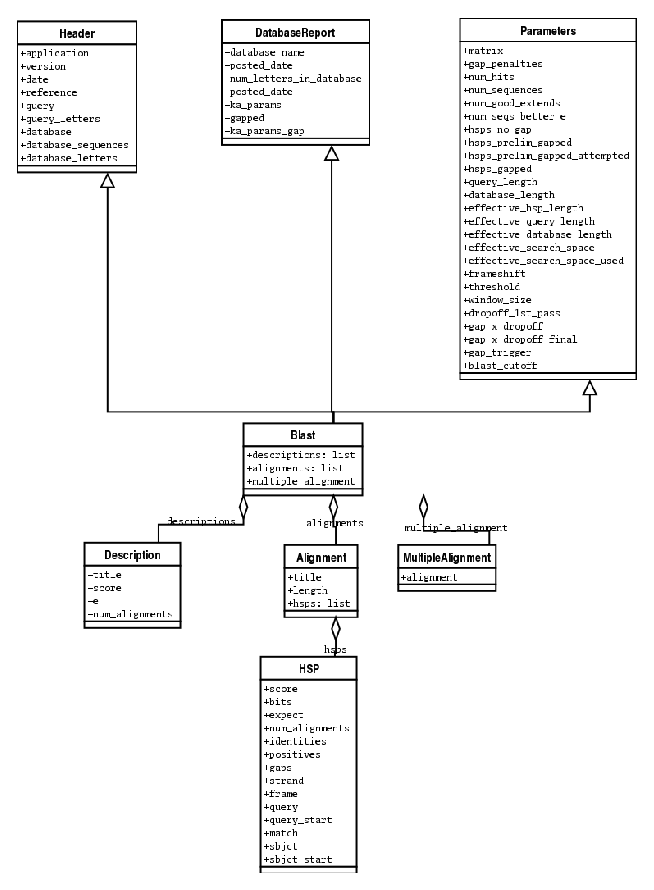
\includegraphics[width=0.8\textwidth]{images/BlastRecord}
\caption{BLAST �Υ�ݡ�����ξ����ɽ�����Ƥ��� Blast Record �Υ��饹��}
\label{fig:blastrecord}
\end{figure}
%\end{latexonly}


\class{PSIBlast} �쥳���ɥ��֥������Ȥ��ɤ����Ƥ��ޤ�����
\program{PSIBlast} �η����֤��Υ��ƥåפ��Ѥ����� \var{rounds}
�򥵥ݡ��Ȥ��Ƥ��ޤ���\class{PSIBlast} �Υ��饹�ޤ��
\ref{fig:psiblastrecord} �˼����ޤ���

%\begin{htmlonly}
%\label{fig:psiblastrecord}
%\imgsrc[width=650, height=750]{images/PSIBlastRecord.png}
%\end{htmlonly}

%\begin{latexonly}
\begin{figure}[htbp]
\centering
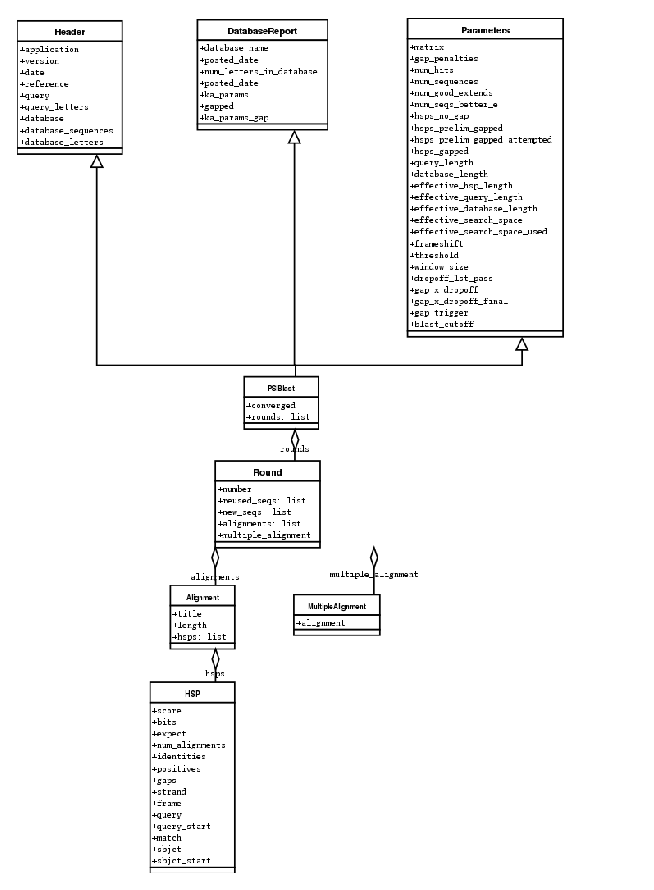
\includegraphics[width=0.8\textwidth]{images/PSIBlastRecord}
\caption{PSIBlast Record ���饹�Υ��饹��}
\label{fig:psiblastrecord}
\end{figure}
%\end{latexonly}

\subsection{��������� BLAST �����餻��}

����򸡺������оݤȤʤ�ǡ����١����򼫺�����ʤ顤��������Ǥ�
\program{BLAST} �μ¹Ԥ��ޤ��ˤ�����ˡ�Ǥ�������饤��Ǥ�
\program{BLAST} ��Ʊ�͡�Biopython �Ǥϥ�����ץȤ����������� 
\program{BLAST} �¹Է�����ƤӽФ��������餷�������ɤ������󶡤��Ƥ��ꡤ
\program{BLAST} �¹Է������󶡤��Ƥ����¿���Υ��ޥ�ɥ饤�󥪥ץ����
�����ƥ��������Ǥ���褦�ˤʤäƤ��ޤ���
�͡��ʥץ�åȥե���������Υ���ѥ���ѤߤΥ�������¹���
\program{BLAST} �ϡ�
\url{ftp://ncbi.nlm.nih.gov/blast/executables/} �Ǽ������ޤ���
�ޤ���NCBI toolbox (\url{ftp://ncbi.nlm.nih.gov/toolbox/}) ����
��ʬ�ǥ���ѥ��뤷�Ƥ�����Ǥ��ޤ���

��������Ǥ�\program{BLAST} �¹Ԥ����뤿��Υ����ɡ��Ȥ�櫓
\function{blastall} ��\function{blastpgp} �Ȥ��ä��ؿ��ϡ�
\module{Bio.Blast.NCBIStandalone} �ˤ���ޤ��������δؿ���
����̾�������ץ������¹Է������б����Ƥ��ޤ���

�����δؿ���Ȥäƥ�������Υǡ����١������Ф���\program{blastall}
��¹Ԥ�����̤��֤����Ƥߤޤ��礦���ޤ���\program{blast} ��¹Ԥ��뤿
���ɬ�פʥѥ������ꤷ�Ƥ����ޤ��礦���ΤäƤ����ͤФʤ�ʤ��Τϡ�
(\program{formatdb} ���Ѱդ��Ƥ������Ϥ���) �����оݤȤ���ǡ����١���
�ؤΥѥ���������������������ä��ե�����ؤΥѥ���������
\program{blastall} �¹Բ�ǽ�����ؤΥѥ����̤�ɬ�פ�����ޤ���

\begin{verbatim}
import os

my_blast_db = os.path.join(os.getcwd(), 'at-est', 'a_cds-10-7.fasta')
my_blast_file = os.path.join(os.getcwd(), 'at-est', 'test_blast',
                             'sorghum_est-test.fasta')
my_blast_exe = os.path.join(os.getcwd(), 'blast', 'blastall')
\end{verbatim}

���ƤΥѥ������ꤷ���Τǡ�\program{blast} ��¹Ԥ��Ʒ�̤���Ф�
�����������ޤ�����������Ԥ�\program{blast} ��¹Ԥ��ޤ�:

\begin{verbatim}
from Bio.Blast import NCBIStandalone

blast_out, error_info = NCBIStandalone.blastall(my_blast_exe, 'blastn',
                                                my_blast_db, my_blast_file)
\end{verbatim}

���������\program{blast} �ץ��������Ф��� Biopython ��
���󥿥ե������ϡ���Ĥ��ͤ��֤��Ƥ��뤳�Ȥ����դ��Ƥ���������
�ǽ������ͤ�\program{blast} �ν��Ϥ��Ф���ϥ�ɥ�ǡ�
��¸������ѡ������Ϥ�����Ǥ��ޤ�������ܤ�����ͤϡ�\program{blast}
���ޥ�ɤ��������뤳�Ȥ����륨�顼���Ϥ�����ޤ���

���顼����μ�갷�������Ǥ����Ȥ����Τϡ����顼��¸�ߤ��ʤ�����
\code{error_info.read()} ��¹Ԥ��褦�Ȥ���ȡ�\function{read}
�ν������֥��å�����Ƥ��ޤä��ͤ��֤��ʤ�����˥�����ץȤ�
��ߤ��Ƥ��ޤ�����Ǥ�����ιͤ��Ǥϡ�\code{blast_out} ��
�֤��줿��̤���Ϥ��Ƥⲿ�������ʤ��ä����ˤΤߥ��顼��
���Ϥ�������ʳ��ξ��ˤϲ��⤻���ۤ��äƤ����Τ������顼��
���ޤ���갷�����֤�����ˡ�Ǥ���

��̤���Ϥ������˥ե��������¸���Ƥ������ȻפäƤ���ʤ顤
���� WWW \program{blast} ����򻲾Ȥ��ơ�\module{copy} �⥸�塼���
�Ȥ����ˤĤ���Ĵ�٤Ƥ������ɤ��Ǥ��礦��

���ơ����Ϥ�������ä��Τǡ����β��Ϥ�Ԥ�ͤФʤ�ޤ���͡�
�Ǥ�����ɤ߿ʤ�ǡ���������Ǽ¹Ԥ���\program{BLAST} �ν��Ϥ���Ϥ���
��ˡ�ˤĤ��ƳؤӤޤ��礦��

\subsection{�������� BLAST �ν��Ϥ���Ϥ���}

�������� \program{BLAST} ������������Ϥϡ�web �١�����\program{BLAST}
�ν��ϤȤϰ�äƤ���Τǡ�\module{Bio.Blast.NCBIStandalone} ���äƤ���
�ѡ�����ȤäƷ�̤�������ޤ���

WWW blast �ξ���Ʊ�� (���Ҥξ���򻲾Ȥ��Ƥ�������)��
�ѡ����˽��Ϥ��Ϥ��ˤϡ��ϥ�ɥ륪�֥������Ȥ���äƤ��ʤ����
�ʤ�ޤ��󡥥ϥ�ɥ륪�֥������Ȥ� \function{readline} �᥽�åɤ�
�������Ƥ��ơ��������������ν�����ԤäƤ���ʤ���Фʤ�ޤ���
���������ϥ�ɥ�����뤿��ˤ褯�Ȥ�������ϡ�\function{blastall}
��\function{blastpgp} �Τ褦�ʡ�Biopython ���󶡤��Ƥ���ؿ���Ȥä�
��������\program{BLAST} ��¹Ԥ��뤫��\program{blast} ��
���ޥ�ɥ饤��ǥ�������˼¹Ԥ��ơ��ʲ��Τ褦�ʥ����ɤ�¹Ԥ��ޤ�:

\begin{verbatim}
blast_out = open('my_file_of_blast_output', 'r')
\end{verbatim}

WWW \program{blast} ��Ʊ���褦�ˡ��̤� Biopython ���ص��ؿ���
�虜�虜�Ȥ�ɬ�פϤ���ޤ���

���ơ��ϥ�ɥ뤬������ä��Τǡ�(�ʸ夳��� \code{blast_out} ��
�Ƥ֤��Ȥˤ��ޤ�) �����Ϥ���Ϥ���������Ǥ��ޤ��������Ϥβ��Ϥ�
�ʲ��Τ褦�ʥ����ɤǹԤ��ޤ�:

\begin{verbatim}
from Bio.Blast import NCBIStandalone

b_parser = NCBIStandalone.BlastParser()
b_record = b_parser.parse(blast_out)
\end{verbatim} 

���Υ����ɤ�¹Ԥ���ȡ�\program{BLAST} ������������ݡ��Ȥ���Ϥ��ơ�
\module{Blast} \class{Record} ���饹 (���Ϥ��Ƥ�����Ϥ�
���Ƥˤ�äơ�\class{Record} ���饹�� Blast �Ѥ� PSIBlast �Ѥ�
�ɤ��餫�ˤʤ�ޤ�) ������������������ǡ�������Ф���褦��
���Ƥ���ޤ����������Ǥϡ�������Ͱʾ�Υ��饤��������Ƥ��Ф���
��ñ�ʥ��ޥ����Ϥ��Ƥߤޤ���


\begin{verbatim}
E_VALUE_THRESH = 0.04
for alignment in b_record.alignments:
    for hsp in alignment.hsps:
        if hsp.expect < E_VALUE_THRESH:
            print '****Alignment****'
            print 'sequence:', alignment.title
            print 'length:', alignment.length
            print 'e value:', hsp.expect
            print hsp.query[0:75] + '...'
            print hsp.match[0:75] + '...'
            print hsp.sbjct[0:75] + '...'
\end{verbatim}

WWW �� �� BLAST �ˤ�������ϲ��ϤˤĤ��Ƥ���򤹤Ǥ��ɤ�Ǥ���С�
�嵭�����ɤ��������������Ƥ�Ʊ�����ȵ��Ť��Ǥ��礦�����餫��
���Ϥ���Ϥ��� \class{Record} ���饹�ˤ����顤��ϸ�����
\program{BLAST} �ν��Ϸ����˴ط��ʤ���갷����ΤǤ���
�ޤä��������餷����

�ְ�ĤΥ쥳���ɤ���ϤǤ���ΤϳΤ��ˤ��������ɡ�����������
�����쥳���ɤ����ä�\program{BLAST} ���ϥե�������ä���ä������͡�
-- ����äƤɤ���ä����������ϤǤ����?�׿��ۤ�̵�ѡ�������
������ˤ���ޤ���


\subsection{BLAST �ν��ϤǤ��äѤ��Υե��������Ϥ���}

����������������������ޤȤ�ˤ��ƥǡ����١��������ơ�
���Ƥ�������Ф��Ƥ褯�Ǥ�����ݡ��Ȥ���Ф���Ȥ������Ǥϡ�
�������� \program{blast} �Ϥ褯�Ǥ��Ƥ��ޤ���
�Ǥ����顤Biopython �ˤϡ��ϼ��Ǥ����ե��������������
Ǻ�ޤ��줺�˲��Ϥ��뵡ǽ������ޤ���

����ʥե�����β��Ϥϡ�blast ���ƥ졼�� (blast iterator)
���Ѥ��ƹԤ��ޤ������ƥ졼����Ȥ���褦�ˤ���ˤϡ��ޤ�
�ѡ��������ꤷ�ơ�blast �ν��ϥ�ݡ��Ȥ���Ϥ��� Blast 
\class{Record} ���֥������Ȥˤ��ޤ�:

\begin{verbatim}
from Bio.Blast import NCBIStandalone

b_parser = NCBIStandalone.BlastParser()
\end{verbatim}

���ˡ������췲�� blast �쥳���ɤ��Ф���ϥ�ɥ뤬�긵�ˤ����
���ꤷ�ơ������ \code{blast_out} �ȸƤ֤��Ȥˤ��ޤ���
�ϥ�ɥ�μ����ˤĤ��Ƥϡ���� blast ���Ϥβ��Ϥ˴ؤ������
�ܤ����Ҥ٤Ƥ��ޤ���

�ѡ�����ϥ�ɥ뤬������ä��Ȥ����ǡ��ʲ��Τ褦�ʥ��ޥ�ɤ�¹�
����С����ƥ졼��������Ǥ��ޤ�:

\begin{verbatim}
b_iterator = NCBIStandalone.Iterator(blast_out, b_parser)
\end{verbatim}

����ܤΥ��ץ����\code{b_parser} �ϥ��ץ����Ǥ���
�ѡ�������ꤷ�ʤ���С����Υ��ƥ졼�������� BLAST ��ݡ��Ȥ�
��İ���֤��Ƥ椭�ޤ���

���ƥ졼����������ä��顤(�ѡ�������������) blast �쥳���ɤ�
\function{next} �Ǽ��Ф��ޤ�:

\begin{verbatim}
b_record = b_iterator.next()
\end{verbatim}

���ƥ졼����\function{next} ��ƤӽФ����Ӥ˿������쥳���ɤ���
�֤��ޤ���
���ơ����Υ쥳�������Τˤ錄�ä�ȿ����� (iteration) ��Ԥ���
����������� blast ����ݡ��Ȥ�����Ǥ��ޤ�:

\begin{verbatim}
while 1:
    b_record = b_iterator.next()

    if b_record is None:
        break

    E_VALUE_THRESH = 0.04
    for alignment in b_record.alignments:
        for hsp in alignment.hsps:
            if hsp.expect < E_VALUE_THRESH:
                print '****Alignment****'
                print 'sequence:', alignment.title
                print 'length:', alignment.length
                print 'e value:', hsp.expect

                if len(hsp.query) > 75:
                    dots = '...'
                else:
                    dots = ''
                
                print hsp.query[0:75] + dots
                print hsp.match[0:75] + dots
                print hsp.sbjct[0:75] + dots
\end{verbatim}

�쥳���ɤ���Ϥ����äƤ��ޤ���\code{b_iterator.next()} ��
\code{None} ���֤����Ȥ����դ��Ƥ�������������ˤ�äơ�
�쥳���ɤ�¸�ߤ��뤫Ĵ�٤ʤ���\keyword{while} �롼�פ�¹Ԥ���С�
��ñ�˥ե��������Τˤ錄�ä�ȿ�������Ǥ��ޤ���

���ƥ졼����Ȥ��ȡ������оݤ���٤˰�ñ�̤Ť��ɤ߹���Τǡ������
blast �쥳���ɤ����������ʤ��˽����Ǥ��ޤ�����Ϥ���
��ǽ��ȤäƤȤ�Ǥ�ʤ��Ф��Ǥ����ե��������������ʤ�
���Ϥ������Ȥ�����ޤ���

\subsection{����ʥե������椫�������ʥ쥳���ɤ�õ��}

�������ƤȤƤ��Բ��˻פ�����ϡ������ BLAST �ե�����򤷤Ф餯��
�ֲ��Ϥ��Ƥ��ơ����θ�ѡ����� \exception{SyntaxError} ����ߤ���
�Ȥ�����ΤǤ�������Ͽ��������Ǥ����Ȥ����Τ⡤
\exception{SyntaxError} ���ѡ���������ʤΤ������뤤�� \program{BLAST}
������ʤΤ���ʬ����ʤ�����Ǥ�������˰������Ȥˡ����顼��̵�뤹��
���Ȥ���Ǥ��ޤ��󡥤Ȥ����Τ⡤�ɤ��Dz��Ϥ����Ԥ����Τ�Ƚ��ʤ��Τǡ�
���顼��̵�뤹��ȥǡ����ν��פʥݥ���Ȥ򸫲ᤴ���Ƥ��ޤ�����
����ʤ�����Ǥ���

���������������򤹤뤿��ˤϤ���äȤ���������ץȤ�񤫤ͤФʤ�ʤ�
�Τ���Ǥ����������� \module{Bio.Blast} �⥸�塼��ˤ�
\class{BlastErrorParser} �����ꡤ��Ȥ������˴�ñ�ˤ��Ƥ���ޤ���
\class{BlastErrorParser} �ϡ��̾�� \class{BlastParser} ��
���ˤ褯���Ƥ��ޤ������ѡ��������Ф���\exception{SyntaxError} 
����­���ơ�������ʬ�Ϥ��褦�Ȼ�ߤ�쥤�䤬�ɲä���Ƥ��ޤ���

���Υѡ����λȤ��������äȸ��Ƥߤޤ��礦 -- �ޤ��������оݤ�
�ե�����ȡ�ȯ����������Υ�ݡ��Ȥ�񤭽Ф�����Υե������������ޤ�:

\begin{verbatim}
import os
 
b_file = os.path.join(os.getcwd(), 'blast_out', 'big_blast.out')
error_file = os.path.join(os.getcwd(), 'blast_out', 'big_blast.problems')
\end{verbatim}

������\class{BlastErrorParser} ��ɬ�פˤʤ�ޤ�:

\begin{verbatim}
from Bio.Blast import NCBIStandalone

error_handle = open(error_file, 'w')

b_error_parser = NCBIStandalone.BlastErrorParser(error_handle)
\end{verbatim}

�ѡ������ϥ�ɥ�򥪥ץ����ΰ����Ȥ��Ƽ�äƤ��뤳�Ȥ�����
���Ƥ����������ϥ�ɥ���Ϥ��ȡ��ѡ�����\exception{SyntaxError}
�����Ф��� \program{blast} �����ƤΥ쥳���ɤ򤳤Υϥ�ɥ��
�񤭽Ф��ޤ����ϥ�ɥ�����ꤷ�ʤ���С����������쥳���ɤ�
��Ͽ����ޤ���

���ơ�\class{BlastErrorParser} ���̾��\program{blast} �ѡ�����
�褦�˻Ȥ��ޤ����Ȥ�櫓��\program{blast} �쥳�������Τˤ錄�ä�
���顼�ѡ�����Ȥäư�ĤŤĥ쥳���ɤ���Ϥ��뤿��˥��ƥ졼����
�������褦�Ȥ��Ƥ⤫�ޤ��ޤ���:

\begin{verbatim}
blast_out = open(b_file)
iterator = NCBIStandalone.Iterator(blast_out, b_error_parser)
\end{verbatim}

���˽Ҥ٤��褦�ˡ����������쥳���ɤϰ��٤˰�ĤŤ��ɤ߽Ф��ޤ���
�����������٤� \program{Blast} �˵������� (���ġ��ѡ������Τ�
�������ʤ�) ���顼����­���ơ�ɬ�פʽ�����Ԥ��ޤ�:

\begin{verbatim}
try:
    next_record = iterator.next()
except NCBIStandalone.LowQualityBlastError, info:
    print "LowQualityBlastError detected in id %s" % info[1]
\end{verbatim}

�����Ǥϡ�\class{BlastErrorParser} �ϰʲ��Τ褦�ʥ��顼�������Ǥ��ޤ�:


\begin{description}
\item [SyntaxError] -- �̾�� \class{BlastParser} ����������Τ�
Ʊ�����顼�ǡ��ѡ���������Υե��������ϤǤ��ʤ����Ȥ˵�������
���顼�Ǥ������Υ��顼���̾�ѡ����ΥХ������ȤäƤ���\program{BLAST}
�ΥС������ȡ��ѡ����������Ǥ���\program{BLAST} �ΥС�������
�԰��פΤ����줫�������Ǥ���

\item [LowQualityBlastError] -- �Ҥɤ��ʼ��ΰ������� 
(�㤨�С�����Ū��ñ��γ˻���Ϣ�ʤ꤫�鹽������Ƥ���褦��û������)
�� BLAST �˳ݤ��褦�Ȥ���ȡ�\program{BLAST} ���������Τ�ޥ�������
���ޤ������Ū�˲����оݤ�����ʤ��ʤäƤ��ޤ����Ȥ�����ޤ���
���ξ�硤���Ƥ����ڤ줿��ݡ��Ȥ����Ϥ��졤�ѡ�����
\exception{SyntaxError} ��Ф��Ƥ��ޤ��ޤ��������������ˤ�
\exception{LowQualityBlastError} �����Ф��ޤ������Υ��顼�ϡ�
�ʲ��Τ褦�ʹ��ܤ򥨥顼����Ȥ����֤��ޤ�:
  \begin{description}
    \item [\code{item[0]}] -- ���顼��å������Ǥ���
    \item [\code{item[1]}] -- ���顼�θ����Ȥʤä����ϥ쥳���ɤ� id 
�Ǥ������ι��ܤϡ����������������Ƥ���쥳���ɤ����Ƶ�Ͽ����
�����������ˤȤƤ�ͭ�ѤǤ���
  \end{description}
\end{description}

��˽Ҥ٤��褦�ˡ����顼��������ȡ�\class{BlastErrorParser} ��
����򵯤����Ƥ���쥳���ɤ�\code{error_handle} �˽񤭽Ф��ޤ���
����\code{error_handle} �����Ƥ�Ĵ�٤ơ���ʬ�λפä��褦�������
�����Ǥ��ޤ���ñ��� \program{blast} ��ݡ��Ȥ�Ȥäƥѡ�����
�ǥХå��Ǥ���Ǥ��⤷��ޤ��󤷡�blast �μ¹Ԥ������Ƥ����꤬
���Ĥ��뤫���Τ�ޤ��󡥤�����ˤ��Ƥ⡤�����餯ͭ�յ����θ���
�ʤ뤳�ȴְ㤤�ʤ��Ǥ�!

\class{BlastErrorParser} ��Ȥ��С������ \program{blast} �ե������
�ǥХå�����������äȳڤˤʤ�Ϥ��Ǥ���


\subsection{PSIBlast ���}

\program{PSIBlast} �򥹥���ץȤ����ñ��ľ�����Ǥ���褦�ˤ���
�ˤϡ�(���饤����ȷ�̤��顤Ŭ�ڤʷ����� align �ե��������Ϥ褦��)
�����ɤ򿧡��Ƚ񤤤Ƥ����ͤФʤ�ޤ��󡥤ޤ��� \program{PSIBlast} ��
�褯Ĵ�٤ơ����ޤ������ˡ��פ��Ĥ�ɬ�פ�����ޤ�...

% 
\section{SWISS-PROT}
\label{sec:swiss-prot}

\subsection{SWISS-PROT �Υ쥳���ɤ����ꤹ��}

SwissProt (\url{http://www.expasy.ch/sprot/sprot-top.html}) ��
����ѥ�����Υǡ����١����ǡ��������ƤϿͼ�ˤ�ä��Խ�����Ƥ��ޤ���
������ץȤ��� SWISS-PROT ����³������ˡ�ȡ�
SWISS-PROT �������֤�����̤�ʸ���Ϥ�����ˡ�򸫤Ƥߤޤ��礦��

�ǽ�ˡ���ʸ���Ϥ����оݤΥǡ����򤤤��Ĥ����Ф��Ƥ���ɬ�פ�����ޤ���
���Υ��륳��������� (chalcone synthase) �����ܤ��Ƥ���Ȥ��ޤ��礦
(�ʤ���̣�����������˵��褦�Ȥ��Ƥ��뤫�� ~\ref{sec:orchids} ��
���Ȥ��Ƥ�������)�����륳��������Ǥϡ���ʪ�Υե�ܥΥ��ɤ���������
�ط����Ƥ��ޤ����ե�ܥΥ��ɤ���ϡ������� UV �ݸ�ޤʤɤ�¿����
�����餷�����ʤ���������ޤ���

SwissProt �Ǹ�����Ԥ��ȡ����륳��������Ǥ˴ؤ�����ͳ��Υ���ѥ���
ID O23729, O23730, O23731 �����Ĥ���Ϥ��Ǥ���
�Ǥϡ�������ץȤ�񤤤ơ������Υ���ѥ��˴ؤ���ǡ��������ꤷ��
�ǡ�����ʸ���Ϥ������򤽤��ʾ������Ф��Ƥߤޤ��礦��

�ޤ��� \module{Bio.WWW.Expasy} �� \function{get_sprot_raw} �Ȥ����ؿ�
��ȤäƤ����Υ쥳���ɤ����ꤷ�ޤ���
���δؿ��ϤȤƤ������餷���� id �����Ϥ���ȡ����̤Υƥ����ȷ�����
�쥳���ɤ��֤��ޤ� (html �Ƕ�ϫ���ʤ��Ƥ��ߤޤ�!)��

��Ū�� 3 �ĤΥ쥳���ɤ������줿�顤1 �Ĥ��礭��ʸ����Ȥ��ƤޤȤᡤ
�Ĥ��ˤ���ʸ������ᤵ���ޤ������񤤤����Ȥ��Τ�Τ����ʲ��˼���
�����ɤǼ¸��Ǥ��ޤ�:

\begin{verbatim}
from Bio.WWW import ExPASy

ids = ['O23729', 'O23730', 'O23731']

all_results = ''
for id in ids:
    results = ExPASy.get_sprot_raw(id)
    all_results = all_results + results.read()
\end{verbatim}

���ơ�Expasy �Ǥθ�����̤����ꤷ���Τǡ����η�̤�ʸ���Ϥ��ƶ�̣��
���������Ф������������ޤ�����¾��¿���Υѡ�����Ʊ���褦�ˡ�
���ƥ졼���ȥѡ����򥻥åȥ��åפ��ޤ����������Ѥ���ѡ����� SwissProt
�ե������ʸ���Ϥ��ƥ쥳���ɥ��֥������Ȥ��Ѵ����ޤ����쥳���ɤǤϡ�
��̣���оݤȤʤ�°������ (feature) �����֥������Ȥ�°���ˤʤäƤ��ޤ�:

\begin{verbatim}
from Bio.SwissProt import SProt
from Bio import File

s_parser = SProt.RecordParser()
s_iterator = SProt.Iterator(File.StringHandle(all_results), s_parser)
\end{verbatim}

�ѡ����ǹ�ʸ���Ϥ�Ԥ����ˡ�ʸ����� \var{all_results} ��ϥ�ɥ�
(handle) ���Ѵ����Ƥ��뤳�Ȥ����դ��Ƥ������������ƥ졼�������ϥǡ���
���ԤŤ��ɤ߹����褦�ˤ��뤿��ˡ����ƥ졼���ˤϥϥ�ɥ���Ϥ��ͤ�
�ʤ�ޤ���
\module{Bio.File} �⥸�塼��ˤϡ�\function{StringHandle} �Ȥ����褯
�Ǥ��������ʴؿ������ꡤʸ�����ϥ�ɥ���Ѵ����Ƥ���ޤ���
�����餷��! ����ǡ��������Ф�������������ޤ�����

�������Ф�����ˡ����ƥ졼����Ȥäơ����ƤΥ쥳���ɤ���
���ɤ�ޤ��������Ǥϡ��ƥ쥳���ɤ��Ф��ơ�ñ�ˤ���äȤ������ޥ�����
ɽ�����ޤ��礦:

\begin{verbatim}
while 1:
    cur_record = s_iterator.next()

    if cur_record is None:
        break

    print "description:", cur_record.description
    for ref in cur_record.references:
        print "authors:", ref.authors
        print "title:", ref.title

    print "classification:", cur_record.organism_classification
    print
\end{verbatim}

��Υ����ɤϡ��ʲ��Τ褦�ʥ��ޥ����Ϥ��ޤ�:

\begin{verbatim}
description: CHALCONE SYNTHASE 8 (EC 2.3.1.74) (NARINGENIN-CHALCONE SYNTHASE 8)
authors: Liew C.F., Lim S.H., Loh C.S., Goh C.J.;
title: "Molecular cloning and sequence analysis of chalcone synthase cDNAs of
Bromheadia finlaysoniana.";
classification: ['Eukaryota', 'Viridiplantae', 'Embryophyta', 'Tracheophyta', 
'Spermatophyta', 'Magnoliophyta', 'Liliopsida', 'Asparagales', 'Orchidaceae', 
'Bromheadia']
\end{verbatim}

SwissProt �쥳���ɤ���¾�ξ������Ф�������С�Ʊ���褦�˴�ñ��
�Ԥ��ޤ���

\section{PubMed}
\label{sec:pub-med}

\subsection{PubMed �˥��������������}

���ʬ��뤤�ϥҥȤ˴ؿ�������ʤ� (���Ȥ������Ǥʤ��Ƥ⡤�ۤȤ�ɤ�
���!)��PubMed (\url{http://www.ncbi.nlm.nih.gov/PubMed/}) ��������
�����ͥ�줿���󸻤ˤʤ�Ǥ��礦���Ǥ����顤¾�ξ����Ʊ���褦�ˡ������Ǥ� 
Python ������ץȤ�Ȥäƾ����������ƻȤ���褦�ˤʤꤿ���Ǥ��͡�

Biopython ���Ѥ��� PubMed �˥����������Τϴ�ñ�Ǥ������˴ط��Τ���
���٤Ƥ�ʸ�� ID (article id) ����������С��ʲ��Τ��ä� 3 �ԤΥ�����
����ɬ�פ���ޤ���:

\begin{verbatim}
from Bio import PubMed

search_term = 'orchid'
orchid_ids = PubMed.search_for(search_term)
\end{verbatim}

���Υ����ɤϡ����˴ؤ��뤹�٤Ƥ�ʸ�� ID �� python �Υꥹ�ȤȤ���
�֤��ޤ�:


\begin{verbatim}
['11070358', '11064040', '11028023', '10947239', '10938351', '10936520', 
'10905611', '10899814', '10856762', '10854740', '10758893', '10716342', 
...
\end{verbatim}

���� ID �ꥹ�Ȥ������顤�ƥ쥳���ɤ������������ϴ�λ�Ǥ��������
�ʤߤޤ��礦��

\subsection{PubMed �Υ쥳���ɤ����ꤹ��}

����Ǥϡ���Ϣ�� ID �����������ˡ���������ޤ�����
ID �����ꤷ���顤���ϳ� ID �˴ط��Τ��� MEDLINE �Υ쥳���ɤ����ꤷ�ơ�
��������������Ф������ȹͤ���Ǥ��礦��

PubMed ����쥳���ɤ���Ф��륤�󥿡��ե������ϡ�Python �ץ�����ޡ���
�ȤäƤϤȤƤ�ľ��Ū�ʤϤ� -- Python �ˤ����뼭�񷿤Υ�ǥ벽 -- �Ǥ���
���Υ��󥿡��ե������򥻥åȥ��åפ���ˤϡ�PubMed �������������̤�
��ʸ���Ϥ��뤿��Υѡ�����ɬ�פǤ����ʲ��Υ����ɤǡ����ƤΥ��åȥ��å�
��Ԥ��ޤ�:

\begin{verbatim}
from Bio import PubMed
from Bio import Medline

rec_parser = Medline.RecordParser()
medline_dict = PubMed.Dictionary(parser = rec_parser)
\end{verbatim}

�����ǹԤä��Τϡ�����饤���ʥ��֥������Ȥ� \var{medline_dict} �κ���
�Ǥ���ʸ�����������ˤϡ�\code{medline_dict[id_to_get]} �Τ褦�ˤ���
�����������ޤ�����������Ԥ��ȡ� PubMed ����³����õ���Ƥ���ʸ����
���Ĥ���ʸ�������ʸ���Ϥ��ƥ쥳���ɥ��֥������Ȥ��Ѵ������֤��ޤ���
�ʤ�Ƹ�����Ǥ��礦! 


���ơ����������餷�����񥪥֥������Ȥ�ɤ��Ȥ��С����� ID ���餢�����
����ϤǤ��뤫���Ƥߤޤ��礦��ɬ�פʺ�Ȥϡ�ñ�˼긵�� ID (���������
���� \var{orchid_ids} �ˤˤ錄�äƥ롼�פ�����̣���оݤȤʤ�����ɽ��
��������Ǥ�:


\begin{verbatim}
for id in orchid_ids[0:5]:
    cur_record = medline_dict[id]
    print 'title:', string.rstrip(cur_record.title)
    print 'authors:', cur_record.authors
    print 'source:', string.strip(cur_record.source)
    print
\end{verbatim}

��Υ����ɤ��Ф�����Ϥϰʲ��Τ褦�ˤʤ�ޤ���

\begin{verbatim}
title: Sex pheromone mimicry in the early spider orchid (ophrys sphegodes):
patterns of hydrocarbons as the key mechanism for pollination by sexual
deception [In Process Citation]
authors: ['Schiestl FP', 'Ayasse M', 'Paulus HF', 'Lofstedt C', 'Hansson BS', 
'Ibarra F', 'Francke W']
source: J Comp Physiol [A] 2000 Jun;186(6):567-74
\end{verbatim}

��ɮ���٤��ϡ�����̾�Υꥹ�ȤǤ��������ɸ��� Python �ꥹ�ȷ��Ȥ���
�֤���Ƥ��ޤ����������뤳�Ȥǡ�Python ��ɸ��ġ����Ȥä�������
����������Ǥ��ޤ����㤨�С��ʲ��Τ褦�ʥ����ɤ�Ȥ��С���Ϣ�Υ���ȥ�
���Τˤ錄�äƥ롼�פ��ơ���������Ԥ�õ���Ф��ޤ�:


\begin{verbatim}
search_author = 'Waits T'

for id in our_id_list:
    cur_record = medline_dict[id]
    
    if search_author in cur_record.authors:
        print "Author %s found: %s" % (search_author,
                                       string.strip(cur_record.source))
\end{verbatim} 

PubMed �� Medline �Υ��󥿡��ե����������Ϥ����褯����Ƥ��ޤ� -- 
������ɤ�ǡ����äȤ��Υ��󥿥ե������ΰ��ϤȻȤ�����褯���򤷤�
��館�����ȤǤ��礦��

\section{GenBank}


GenBank �쥳���ɷ����ϡ����������˴ؤ���°������ (feature)��
����¾��Ϣ��������ξ����Ͽ������ˡ�Ȥ��ƹ����Ȥ��Ƥ��ޤ���
���η����ϡ�NCBI �Υǡ����١��� (\url{http://www.ncbi.nih.gov/}) 
�����������뤿����ɤ����ʤǤ⤢��ޤ���


\subsection{GenBank �Υ���ȥ�� NCBI �������ꤹ��}

\module{Bio.GenBank} �饤�֥�� �ΤȤƤ���Ũ�ʵ�ǽ�ϡ�����ȥ��
GenBank ���鼫ưŪ�˼����Ǥ���Ȥ����Ȥ����Ǥ���
����ϡ������κ�Ȥ�ư������褦�ʥ�����ץȤ�񤯾�ǤȤƤ�
�����Ǥ����������Ǥϡ�NCBI �ǡ����١����˥����������������������
����쥳���ɤ����ꤹ����ˡ�򼨤��ޤ���

�ޤ��ϥ������������ơ����Ф������쥳���ɤ��Ф��� ID �򸡺�
���ޤ��礦�������Ǥϡ���Τ����������\emph{�����掠�ܥƥ� (Opuntia)}
����˼�äơʤʤ��ʤ�䤬���椷�Ƥ��뤫��Ǥ��ˡ�����äȤ���������
�¹Ԥ��Ƥߤޤ��礦���ʲ��Υ����ɤ�Ȥ��С������å�������Ԥäơ�
���ƤΥ쥳���ɤ��б����� GI (GenBank ���̻�) ������Ǥ��ޤ�:

\begin{verbatim}
from Bio import GenBank

gi_list = GenBank.search_for("Opuntia AND rpl16")
\end{verbatim}

\var{gi_list} �ˤϡ�������˰��פ������٤Ƥ� GenBank ���̻Ҥ���ʤ�
�ꥹ�Ȥˤʤ�ޤ�:

\begin{verbatim}
['6273291', '6273290', '6273289', '6273287', '6273286', '6273285', '6273284']
\end{verbatim}

GI ������Ǥ����Τǡ��� ID ��ȤäƼ��񥤥󥿥ե�������𤷤� NCBI 
�ǡ����١����˥��������Ǥ��ޤ����㤨�С��ǽ�� GI ���Ф�������
��Ф���ʤ顤�ޤ� NCBI �˥����������뼭�񥪥֥������Ȥ���ʤ��Ƥ�
�ʤ�ޤ���:


\begin{verbatim}
ncbi_dict = GenBank.NCBIDictionary()
\end{verbatim}

���񥪥֥������Ȥ��ä��顤���Τ褦�˾������Ф��Ƥߤޤ��礦:

\begin{verbatim}
gb_record = ncbi_dict[gi_list[0]]
\end{verbatim}

������Ǥϡ�\var{gb_record} �� GenBank �����Υ쥳���ɤˤʤ�Ϥ��Ǥ�:

\begin{verbatim}
LOCUS       AF191665      902 bp    DNA             PLN       07-NOV-1999
DEFINITION  Opuntia marenae rpl16 gene; chloroplast gene for chloroplast
            product, partial intron sequence.
ACCESSION   AF191665
VERSION     AF191665.1  GI:6273291
...
\end{verbatim}

������Ǥϡ�ñ�����Υ쥳���ɤ����ꤷ�������Ǥ��������Υ쥳���ɤ�
ľ�ܥѡ������Ϥ��ƹ�ʸ���Ϥ������쥳���ɤ��Ѵ����뤳�Ȥ����ޤ���
�㤨�С� GenBank �ե����뤫����Ф��� \class{SeqFeature}
���֥������Ȥ� \class{SeqRecord} ���֥������Ȥ��ᤷ������С�
�ޤ�\module{GenBank} �� \class{FeatureParser} �Ǽ��񥪥֥������Ȥ�
��������ɬ�פ�����ޤ�:

\begin{verbatim}
record_parser = GenBank.FeatureParser()
ncbi_dict = GenBank.NCBIDictionary(parser = record_parser)
\end{verbatim}

����ǡ��쥳���ɤ���Ф���С��ǤΥƥ����ȷ����Υ쥳���ɤ�
����� \class{SeqRecord} ���֥������Ȥˤʤ�ޤ�:

\begin{verbatim}
>>> gb_seqrecord = ncbi_dict[gi_list[0]]
>>> print gb_seqrecord
<Bio.SeqRecord.SeqRecord instance at 0x102f9404>
\end{verbatim}

GenBank ����ɤ�ʷ������Ѵ��Ǥ��뤫�ˤĤ��Ƥξܺ٤ϡ�
\ref{sec:gb-parsing} ��򻲾Ȥ��Ƥ���������

����������ưŪ�������̼�����ǽ��Ȥ��ȡ����Ȥ���Ϥ뤫��ͭ���ˤ�
��ޤ������ξ塤������ǽ�ˤϰ�����֤��Ȥ˼�����Ԥ� time-delay �Τ褦
����Ũ�ʵ�ǽ���Ȥ߹��ޤ�Ƥ��ơ����ˤʥ��������ˤ�ä� NCBI ���ܤ餻��
����������֥��å������褦�ʤ��Ȥ��ʤ��褦�ˤ��Ƥ��ޤ���

\subsection{GenBank �쥳���ɤ��᤹��}
\label{sec:gb-parsing}

GenBank �ե�����������餷���Ǥ��Ƥ��ơ���������ξ��󤬤��������
��������ǡ��ºݤˤϰ���ˤۤ�ξ����ξ��󤷤����Ф������ʤ�����
����ޤ��󡥤���������Ȥθ��Ȥʤ�Τϡ��ǡ����򤤤��˹�ʸ���Ϥ��뤫��
����
Biopython �Ǥ�ʣ���� GenBank �ѡ������󶡤��Ƥ��ơ�����������Ȥ�
�Ԥ���Ǽ�����Ǥ���褦�ˤ��Ƥ��ޤ�������ޤǤΤȤ�����
\module{GenBank} �Ǥϰʲ��Υѡ������󶡤��Ƥ��ޤ�:


\begin{description}

\item [RecordParser] ���Υѡ������ǤΥ쥳���ɤ�ʸ���Ϥ��ơ� GenBank 
��ͭ�Υ쥳���ɥ��֥������ȷ������Ѵ����ޤ������Υ��֥������ȤǤ�
������ǤΥ쥳���ɤ����˶ᤤ��ǥ�ǰ����Τǡ�ñ�� GenBank ��
�ġ��Υ쥳���ɼ��Τ˶�̣��������ˤϤ��Υѡ�����Ȥ��Τ��褤�Ǥ��礦��

\item [FeatureParser] ���Υѡ������ǤΥ쥳���ɤ�\class{SeqRecord} 
���֥������Ȥ��Ѵ����ޤ���\class{SeqRecord} ���֥������ȤǤϡ�
���Ƥ�°���ơ��֥����\class{SeqFeatures} ��ɽ������Ƥ��ޤ�
(�����Υ��֥������ȤˤĤ��Ƥξܺ٤� \ref{sec:advanced-seq} ��
���Ȥ��Ƥ�������)�����ɸ��Ū�ʷ����Ǿ�������ꤷ�������ˤ�
������Υѡ�����Ȥ��Τ��褤�Ǥ��礦��

\end{description}

�ɤ������ˡ��Ȥ�ˤ��衤���������Υѡ����κǤ����Ū�ʻȤ����ϡ�
���ƥ졼����������ơ�GenBank �쥳���ɤ����ä��ե������ѡ�������
�Ȥ�����Τˤʤ�ޤ������κ�Ȥϡ�¾�Υǡ��������Ǥν�����ˡ������
���Ƥ��ơ��㤨�аʲ��Τ褦�ʥ����ɤˤʤ�ޤ�:


\begin{verbatim}
from Bio import GenBank

gb_file = "my_file.gb"
gb_handle = open(gb_file, 'r')

feature_parser = GenBank.FeatureParser()

gb_iterator = GenBank.Iterator(gb_handle, feature_parser)

while 1:
   cur_record = gb_iterator.next()

   if cur_record is None:
       break

   # now do something with the record
   print cur_record.seq
\end{verbatim}

���Υ����ɤǤϡ�ñ�� GenBank �ե�������Ϥä�ȿ��������Ԥ���
�쥳���ɤ��Ȥ˹�ʸ���Ϥ�Ԥä� SeqRecord �� SeqFeature ���֥������Ȥ�
�Ѵ��������Υ쥳���ɤ������ɽ�� \class{Seq} ���֥������Ȥ�
���Ϥ��ޤ���

¾�η�����Ʊ�͡�GenBank �쥳���ɤ򰷤��ġ��뤬�������󤢤�ޤ���
�����Υġ����Ȥ��� GenBank ��ȤäƤ�ꤿ�����Ȥϲ��Ǥ�Ǥ���
�Ϥ��Ǥ���


\subsection{����� GenBank �ǡ����١������������}

��ʬ�ѤθĿ�Ū�� GenBank �ǡ����١�����������ơ����񥪥֥������Ȥ�
�褦�˥��������Ǥ���Ȥ����ȤƤ������餷����ǽ������ޤ���
(����������餷��������ʵ�ǽ�Ǥ����Ȥ����Τϡ����Υ��������
�ǡ����١����ˤ⡤BioCorba ��Ȥäƥͥåȥ���ۤ��˥�������
�Ǥ��뤫��Ǥ� -- �ܺ٤� BioCorba �Υɥ�����Ȥ򻲾Ȥ��Ƥ�������)

��������ʥǡ����١����κ����Ǥϡ��ޤ�����ǥ����ե������������ơ�
�ե�������γƥ쥳���ɤ����᤯���������Ǥ���褦�ˤ��ޤ���
�����Ԥ��ˤϡ�\function{index_file} �ؿ���Ȥ��ޤ�:

\begin{verbatim}
>>> from Bio import GenBank
>>> dict_file = 'cor6_6.gb'
>>> index_file = 'cor6_6.idx'
>>> GenBank.index_file(dict_file, index_file)
\end{verbatim}

���κ�Ȥǡ� \file{my_index_file.idx} �Ȥ���̾���Υե����뤬����
����ޤ������ơ����Υ���ǥ�����Ȥ��С��ġ��Υ쥳���ɤ˥�������
�Ǥ���褦�ʼ��񥪥֥������Ȥ�����Ǥ��ޤ���
\class{Iterator} �� \class{NCBIDictionary} ���󥿥ե������Τ褦�ˡ�
�ǤΥ쥳���ɤ��ᤷ���ꡤ���񥪥֥������Ȥ�ѡ������Ϥ��ơ��쥳���ɤ�
�֤��������Ƥ�ʸ���Ϥ�������Ǥ��ޤ���
���ξ�硤�쥳���ɤ�������ˤ� \class{FeatureParser} ���Ϥ��Ƥ�����
���θ�� \class{SeqRecord} ���֥������Ȥ�������ޤ���

����ν����ϴ�ñ�ǡ��ʲ��� 1 �Ԥ����Ǥ�:

\begin{verbatim}
>>> gb_dict = GenBank.Dictionary(index_file, GenBank.FeatureParser())
\end{verbatim}

����ǡ�Genbank �Υǡ����򼭽����˰�����褦�ˤʤ�ޤ�����
�㤨��:

\begin{verbatim}
>>> len(gb_dict)
7
>>> gb_dict.keys()
['L31939', 'AJ237582', 'X62281', 'AF297471', 'M81224', 'X55053']
\end{verbatim}

�Ǹ�ˡ�ź��ɽ�� (subscripting) �ǥ��֥������Ȥ���Ф��ޤ�: 

\begin{verbatim}
>>> gb_dict['AJ237582']
<Bio.SeqRecord.SeqRecord instance at 0x102fdd8c>
\end{verbatim}
\section{���饤����Ȳ��Ϥΰ���}

��������󷲤��Ф��ƥ��饤����Ȥ�ݤ�����ȡ��ȤƤ������ʤ��Ȥ�
�褯����ޤ�����ԤϤ����褯�Ȥäơ���äĤ�Ū������֤δ�Ϣ����
Ĵ�٤��ꤷ�ޤ������äơ����饤����Ȥ�ݤ��ơ����η�̤����䤹��
���֥������Ȥ��֤��褦�� Python ������ץȤ򤹤Ф䤯�񤭾夲�����
�����ΤϤȤƤ������餷�����ȤʤΤǤ���Biopython �ˤ����륢�饤�����
��Ϣ�Υ����ɤϡ�Python ��٥뤫�饢�饤����Ȳ��ϥץ������˥�������
�Ǥ���褦�ˤ���������ץȾ夫������ᤤ���饤����Ȳ��Ϥ��ǽ��
���뤿��Τ�ΤǤ���

\subsection{clustalw}
\label{sec:align-clustal}

\program{clustalx}
(\url{http://www-igbmc.u-strasbg.fr/BioInfo/ClustalX/Top.html}) 
�ϡ��ޥ���ץ륢�饤����Ȥ�Ԥ������ͥ�줿�ץ������Ǥ���
Biopython �Ǥϡ�\program{clustalx} ���������� clustal �����Υ��饤����Ⱦ���
(�̾�ϳ�ĥ�� \file{*.aln} ���Ĥ��Ƥ��ޤ�) �˥����������뤿���
��ˡ���󶡤��Ƥ��ޤ����ޤ���\program{clustalx} �Υ��ޥ�ɥ饤���ǤǤ���
\program{clustalw} �ؤΥ����������ʤ��󶡤��Ƥ��ޤ���

\program{clustalw} �Ȥ��Ȥ��Ԥ���Ǥϡ��ޤ��ǽ�Υ��ƥåפȤ��ơ�
�ץ��������Ϥ����ޥ�ɥ饤����������ꤷ�ޤ��� \program{clustalw}
 �ˤ������
���Υ��ޥ�ɥ饤�󥪥ץ���󤬤��ꡤ��������Υѥ�᥿�����ꤹ�뤳�Ȥ�
�ʤ�С�����ʥ��ޥ�ɥ饤������Ϥˤ���˰���Ƥ��ޤ��Ǥ��礦��
���ޥ�ɥ饤�󥯥饹 (command line class) �Ǥϡ�����Ǥ���
���ޥ�ɥ饤�󥪥ץ����򥯥饹��°���Ȥ��ư������Ȥǡ����ޥ�ɥ饤��
���ǥ벽���Ƥ��ޤ�������Υѥ�᥿�����ꤹ�뤿����ص��ؿ���
�����Ĥ����ꡤ�ѥ�᥿����ˤ�����륨�顼�򸡽ФǤ���褦��
�ʤäƤ��ޤ���

\program{clustalw} �ˤ��ޥ���ץ륢�饤����Ȥ�¹Ԥ��뤿���
���ޥ�ɥ饤�󥪥֥������Ȥ��������ˤϡ��ʲ��Τ褦�ˤ��ޤ�:

\begin{verbatim}
import os
from Bio.Clustalw import MultipleAlignCL

cline = MultipleAlignCL(os.path.join(os.curdir, 'opuntia.fasta'))
cline.set_output('test.aln')
\end{verbatim}

�ޤ���\class{MultipleAlignCL} �� import ���ޤ������Υ��饹��
\program{clustalw} �ˤ��ޥ���ץ륢�饤����Ȥμ¹Ԥ��ǥ벽
���Ƥ��ޤ���
���ˡ����Υ��ޥ�ɥ饤�󥯥饹���������ޤ������κݡ�
���饤����Ȥ��оݤˤ��� FASTA �����Υե����������Ȥ���
���ꤷ�ޤ���
������ؿ��ˤϡ����ץ�������������Ȥ��ơ�\program{clustalw}
�μ¹ԥե����뤬����������Ǥ��ޤ����ǥե���ȤǤϡ�
\program{clustalw} ��\envvar{PATH} ��Τɤ����ˤ���Ȳ��ꤷ�ơ�
���ޥ�ɥ饤�󥪥֥������Ȥ�ñ�� \code{'clastalw'} �Ȥ���̾����
�ץ�������ƤӽФ��ޤ���

���ιԤǤϡ���̤ν������ե����� \file{test.aln} �����ꤷ�Ƥ��ޤ���
\class{MultipleAlignCL} ���֥������Ȥˤ�¾�ˤ⤿������Υѥ�᥿
�����ꡤ���Ϥη��������󥮥�åפΥ����ȤȤ��ä������Ԥ��ޤ���

���ޥ�ɥ饤������Ƥϡ�\class{MultipleAlignCL} ��\function{__str__} 
�᥽�åɤ�ƤӽФ�������������ɤ�ޤ����ºݤˤϡ�\code{str(cline)}
�Ȥ����ꡤñ�� \code{print cline} �Ȥ��������ɽ������ޤ���
�����Ǥϡ��ʲ��Τ褦�ʽ��Ϥˤʤ�Ϥ��Ǥ�:

\begin{verbatim}
clustalw ./opuntia.fasta -OUTFILE=test.aln
\end{verbatim}

���ơ���ñ�ʥ��ޥ�ɥ饤�������Ǥ����Τǡ����Υ��ޥ�ɥ饤���
�¹Ԥ��Ʒ�̤���ޤȤᡤ�����Ǥ���褦�ˤ��ޤ��礦��
�������ϡ�\class{Clastalw} ��\function{do_alignment} ��Ȥä�
�ʲ��Τ褦�˹Ԥ��ޤ�:

\begin{verbatim}
from Bio import Clustalw

alignment = Clustalw.do_alignment(cline)
\end{verbatim}

���¹Ԥ���ȡ�Biopython ����ۤ����ꤷ�����ޥ�ɥ饤���¹Ԥ��ơ�
����Υѥ�᥿�� \program{clustalw} �����餻�ޤ�������
\program{clustalw} ����ν��Ϥ�����ߡ�Biopython �����ϤǤ���
���� (���ߤΤȤ��� clustal �����Τ�) �Ǥ���С����Ϥ�Ԥäơ�
Ŭ�ڤʷ��Υ��饤����ȥ��֥������Ȥˤ����֤��ޤ��������Ǥϡ�
��̤�ǥե���Ȥ� clustal �����ˤ��Ƥ���Τǡ�����ͤΥ��֥�������
\code{alignment} ���֥������Ȥ� \class{ClustalAlignment} ���ˤʤ�ޤ���

\code{alignment} ���֥������Ȥ������顤�㤨�Х��饤��������
���Ƥ�������Ф���\class{seq_record} ���֥������Ȥ�����Ȥ��ä�
�褦�ʽ�����Ԥ��ޤ�:

\begin{verbatim}
all_records = alignment.get_all_seqs()

print 'description:', all_records[0].description
print 'sequence:', all_records[0].seq
\end{verbatim}

��Υ����ɤ�¹Ԥ���ȡ����饤����Ȥκǽ�����󥪥֥������Ȥ�
�Ф������� (description) �����󥪥֥������Ȥ���Ϥ��ޤ�:

\begin{verbatim}
description: gi|6273285|gb|AF191659.1|AF191
sequence: Seq('TATACATTAAAGAAGGGGGATGCGGATAAATGGAAAGGCGAAAGAAAGAAAAAAATGAAT 
...', IUPACAmbiguousDNA())
\end{verbatim}

���饤����Ȥκ���Ĺ��׻��Ǥ��ޤ�:

\begin{verbatim}
length = alignment.get_alignment_length()
\end{verbatim}

���饤����ȥ��֥������Ȥ򥪥ꥸ�ʥ�η����ǽ��Ϥ�������С�
ñ�� \function{__str__} �˥���������������Ǥ����Ĥޤꡤ
\code{print alignment} ��¹Ԥ�������Ǥ��ޤ��ޤ���:


\begin{verbatim}
CLUSTAL X (1.81) multiple sequence alignment


gi|6273285|gb|AF191659.1|AF191      TATACATTAAAGAAGGGGGATGCGGATAAATGGAAAGGCGAAAGAAAGAA
gi|6273284|gb|AF191658.1|AF191      TATACATTAAAGAAGGGGGATGCGGATAAATGGAAAGGCGAAAGAAAGAA
...
\end{verbatim}

��������С����ꥸ�ʥ�ξ���˼��ä��뤳�Ȥʤ������饤����ȷ�̤�
�ե�����˴�ñ�˽��᤻�ޤ���

���饤����ȷ�̤�Ȥä�¾�ˤ⤤�������ʤ��Ȥ򤷤Ƥߤ�����С�
���饤����ȷ�̤�\class{SummaryInfo} ���֥�������
�Τ褦�ʥ��饤����Ⱦ����������֥������Ȥ��Ϥ��Τ��٥��ȤǤ���
����ˤĤ��Ƥ�\ref{sec:summary-info} ����������ޤ���

\subsection{���ޥ����λ���}
\label{sec:summary-info}

���饤����ȷ�̤������顤���Ϥ�������������Ф����Ȥ���
�Ϥ��Ǥ��͡�Biopython �Ǥϡ����륢�饤����Ⱦ���˴ؤ������Ƥξ����
��������褦�ʰ�Ϣ�δؿ������ƥ��饤����ȥ��֥������Ȥ˻�������
����ˡ�����������ǽ�򥢥饤����ȥ��֥������Ȥ���������̤�
���饹��ʬΥ���褦�Ȼ�ߤƤ��ޤ���

���饤����ȥ��֥������Ȥ��饵�ޥ����򻻽Ф�������ϤȤƤ�
��ñ�Ǥ����㤨�С�\code{alignment} �Ȥ���̾���Υ��֥������Ȥ�
����Ȥ��ޤ��礦�����ޥ����򻻽Ф��륪�֥������Ȥ�������ɬ�פʤΤ�
��������Ǥ�:

\begin{verbatim}
from Bio.Align import AlignInfo
summary_align = AlignInfo.SummaryInfo(alignment)
\end{verbatim}

\code{summary_align} �ϤȤƤ������ʥ��֥������Ȥǡ��ʲ��Τ褦��
����������������ԤäƤ���ޤ�:

\begin{enumerate}
  \item ��ñ�ʥ��󥻥󥵥�����η׻� -- \ref{sec:consensus} �Ỳ��
  \item �����ð�Ū���������� (position specific score matrix) �η׻�
    -- \ref{sec:pssm} �Ỳ��
  \item �����̤η׻� -- \ref{sec:getting-info-content} �Ỳ��
  \item �Ĵ��ִ���������� -- ���ε�ǽ��
    �Ȥä��ִ���������ˡ�ξܺ٤�\ref{sec:sub-matrix} �Ỳ��
\end{enumerate}

\subsection{��ñ�ʥ��󥻥󥵥�����η׻�}
\label{sec:consensus}

\ref{sec:summary-info} ��Dz��⤵��Ƥ���\class{SummaryInfo} 
���֥������ȤǤϡ����饤����Ȥˤ������ñ�ʥ��󥻥󥵥�����
��׻����뵡ǽ���󶡤��Ƥ��ޤ���\code{summary_align} �Ȥ���̾����
\class{SummaryInfo} ���֥������Ȥ����Ƥ���Ȥ��ơ����󥻥󥵥������
�׻��ϰʲ��Τ褦�ˤ��ƹԤ��ޤ�:


\begin{verbatim}
consensus = summary_align.dumb_consensus()
\end{verbatim}

̾������������褦�ˡ����δؿ����Ԥ��Τ������˴�ñ�ʥ��󥻥󥵥��׻�
�ǡ����󥻥󥵥���ʬ�γ��������ƤλĴ��ȹ礷���Ǥⶦ�����ι⤤�Ĵ��
�ͤ����� (�ǥե���Ȥ� 0.3) ���⤤�ͤ���ľ��ˡ����λĴ��
���󥻥󥵥�������ɲä��ޤ���
���ͤ�ã���ʤ���С�ۣ��ʻĴ��ɽ��ʸ���򥳥󥻥󥵥�������ɲ�
���ޤ�������ͤΥ��󥻥󥵥������ \class{Seq} ���֥������Ȥǡ�����
����ե��٥åȤϥ��󥻥󥵥��������Ȥ����������󤫤��¬���ޤ���
���äơ�\code{print consensus} ��¹Ԥ���ȡ��ʲ��Τ褦�ʽ��Ϥ�
�ʤ�Ϥ��Ǥ�:


\begin{verbatim}
consensus Seq('TATACATNAAAGNAGGGGGATGCGGATAAATGGAAAGGCGAAAGAAAGAAAAAAATGAAT 
...', IUPACAmbiguousDNA())
\end{verbatim} 

���ץ����Υѥ�᥿���Ϥ��ȡ�\function{dumb_consensus} ��ư���
Ĵ���Ǥ��ޤ�:

\begin{description}
\item[����] ���󥻥󥵥�����γ����ˤ����ơ�����λĴ�򥳥󥻥󥵥�
�Ȥ��ƺ��Ѥ��뤿���ɬ�פʻĴ�ζ������Ǥ����ǥե���Ȥ� 0.7 �Ǥ���

\item[ۣ��ʻĴ��ɽ��ʸ��] ۣ��ʻĴ��ɽ���˻Ȥ���ʸ���Ǥ���
�ǥե���Ȥ� \code{'N'} �Ǥ���

\item[���󥻥󥵥�����Υ���ե��٥å�] ���󥻥󥵥�����˻Ȥ�
����ե��٥åȤǤ�������ե��٥åȤ���ꤷ�ʤ���硤���饤�����
�оݤ�����Υ���ե��٥åȤ˴�Ť�����¬���Ԥ��ޤ���
\end{description}

\subsection{�����ð�Ū����������}
\label{sec:pssm}

�����ð�Ū���������� (PSSM, position specific score matrix) 
��Ȥ��ȡ����饤����Ȥξ���򥳥󥻥󥵥��Ȥϰ㤦��ˡ�ǽ���Ǥ���
�͡������Ӥ�ͭ�Ѥʤ��Ȥ�����ޤ���
����Ū�ˤϡ�PSSM ��\emph{�׿�}���� (count matrix) �Ǥ���
PSSM �Ǥϡ����饤����Ȥγƥ����ˤĤ��ơ��ƥ���ե��٥å�ʸ����
���������������פ��ޤ�����׷�̤ϡ����餫����ɽŪ�������
��¦�μ��ˤȤä�ɽ�����ޤ�����������ϥ��󥻥󥵥�����Ǥ��ޤ��ޤ��󤬡�
���饤��������Ǥ�դ�����ˤ�Ǥ��ޤ���

�㤨�С��ʲ��Υ��饤�����:

\begin{verbatim}
GTATC
AT--C
CTGTC
\end{verbatim}

�ξ�硤���� PSSM ��:

\begin{verbatim}
      G A T C
    G 1 1 0 1
    T 0 0 3 0
    A 1 1 0 0
    T 0 0 2 0
    C 0 0 0 3
\end{verbatim}

�Ȥʤ�ޤ���

\code{c_align} �Ȥ���̾���Υ��饤����ȥ��֥������Ȥ������
���ޤ��礦�����󥻥󥵥������¦�μ��ˤ��� PSSM ��׻�����ˤϡ�
�ޤ����饤����Ȥ��Ф��륵�ޥꥪ�֥������Ȥ�������ơ�
���󥻥󥵥������׻����ޤ�:

\begin{verbatim}
summary_align = AlignInfo.SummaryInfo(c_align)
consensus = summary_align.dumb_consensus()
\end{verbatim}

�����ǡ� PSMM ��������뤳�Ȥˤʤ�ޤ������׻�����ݤˤ�
ۣ��ʻĴ�\code{N} ��̵�뤹��褦�ˤ��ޤ�:


\begin{verbatim}
my_pssm = summary_align.pos_specific_score_matrix(consensus,
                                                  chars_to_ignore = ['N'])
\end{verbatim}

����������Ĥ���ޤ�:
Two notes should be made about this:

\begin{enumerate}
  \item ����ե��٥åȤθ�̩����ݻ����뤿��ˡ���μ��ˤϥ��饤�����
���֥������ȤǻȤ��Ƥ��륢��ե��٥å����ʸ���������ѤǤ��ޤ���
����å�ʸ���� PSSM �ξ�μ��ˤ�����ޤ���

  \item ��¦�μ���ɽ����������ˤϡ����󥻥󥵥��Ǥʤ���Τ��Ϥ��Ƥ�
���ޤ��ޤ����㤨�С����饤������������ܤ�����򤳤���ɽ��
��������С��ʲ��Τ褦�ˤ��ޤ�:

\begin{verbatim}
second_seq = alignment.get_seq_by_num(1)
my_pssm = summary_align.pos_specific_score_matrix(second_seq
                                                  chars_to_ignore = ['N'])
\end{verbatim}

\end{enumerate}

���̿���¹Ԥ���ȡ�\class{PSSM} ���֥������Ȥ��֤��ޤ�����ۤɤΤ褦��
PSSM ��ɽ������ˤϡ�ñ�� \code{print my_pssm} ��¹Ԥ��ޤ�����̤�:

\begin{verbatim}
    A   C   G   T
T  0.0 0.0 0.0 7.0
A  7.0 0.0 0.0 0.0
T  0.0 0.0 0.0 7.0
A  7.0 0.0 0.0 0.0
C  0.0 7.0 0.0 0.0
A  7.0 0.0 0.0 0.0
T  0.0 0.0 0.0 7.0
T  1.0 0.0 0.0 6.0
...
\end{verbatim}

�Τ褦�ˤʤ�ޤ���

PSSM �γ����Ǥˤϡ�\code{your_pssm[sequence_number][residue_count_name]} 
�Τ褦��ź������ǥ��������Ǥ��ޤ����㤨�С���� PSSM �ǡ�����ܤ�����
���Ф���Ĵ� \code{'A'} �Υ�����Ȥ�����ˤ�:


\begin{verbatim}
>>> print my_pssm[1]['A']
7.0
\end{verbatim}

�Τ褦�ˤ��ޤ���

���Τ褦�ˡ� PSSM ���饹�ι�¤�ϡ������ð�Ū����������γ����Ǥ�
�����������������򤭤줤�˽��Ϥ�����Ȥ��ä��������ñ�ˤǤ���
�褦�ˤʤäƤ��ޤ���

\subsection{������}
\label{sec:getting-info-content}

�ʲ��β����ˤ������������¸����ɽ����ǽ�������¬�٤ˡ�
������ξ����̤�����ޤ���

ʬ����ʪ�ؼԸ����˽񤫤줿ͭ�Ѥʾ��������������Ȥ��Ƥϡ�
\url{http://www.lecb.ncifcrf.gov/~toms/paper/primer/} ������ޤ���
���饤����Ȳ��Ϥ���Ū�Ȥ�����硤���󥻥󥵥�����䡤������ʬ�����
�����̤�Ĵ�٤뤳�Ȥˤʤ�ޤ���
�ޥ���ץ����󥢥饤������������Υ����ˤ���������̤η׻��ϡ�
�ʲ��μ��ǹԤ��ޤ�:


\begin{displaymath}
IC_{j} = \sum_{i=1}^{N_{a}} P_{ij} * log(\frac{P_{ij}}{Q_{i}}) 
\end{displaymath}

�����ǡ����줾����ѿ��ΰ�̣�ϰʲ��Τ褦�ˤʤäƤ��ޤ�:

\begin{description}
  \item [$IC_{j}$] -- ���饤�������� $j$ ���ܤΥ����ξ����̡�
  \item [$N_{a}$] -- ����ե��٥åȤ�������ʸ���ο���
  \item [$P_{ij}$] -- �������������ʸ�����и��������� (�㤨�С�
���륢�饤����ȤΤ��륫�����ǡ�G �� 6 ���� 3 ��и����Ƥ���С�
�����ͤ� 0.5 �Ǥ�)��
  \item [$Q_{i}$] -- �����ʸ���νи����٤δ����͡����ι�ϥ��ץ�����
���ꡤ���λȤ����ϥ桼���ˤ���ͤ��Ƥ��ޤ����ǥե���ȤǤϡ�
����ѥ�������Ф��ƤϾ�� 0.05���˻�������Ф��Ƥ� 0.25 ��ưŪ��
������Ƥޤ�������ϡ�������Ψʬ�ۤ��Ф��벾�����ڹԤ�ʤ�����
�����̤η׻����������ޤ������餫�λ�����Ψʬ�ۤ��ꤷ�������䡤
��ɸ��Υ���ե��٥åȤ�Ȥ��������ˤϡ��桼���� $Q_{i}$ ���ͤ�
�󶡤��ʤ���Фʤ�ޤ���
\end{description}

���ơ�Biopython �ǤɤΤ褦�˾����̤�׻����Ƥ��뤫�����򤷤��Ȥ����ǡ�
���饤����Ȥ�������ΰ���Ф��ƾ����̤�׻�������ˡ�򸫤Ƥ椭�ޤ��礦��

�ޤ������饤����ȥ��֥������Ȥ�Ȥäƥ��ޥꥪ�֥������Ȥ�������ޤ���
����̾���� \code{summary_align} �Ȥ��ޤ� (���ޥ�μ�����ˡ��
\ref{sec:summary-info} ��򻲾Ȥ��Ƥ�������) �����ޥꥪ�֥������Ȥ�
����줿�顤�����̤η׻��ϴ�ñ�Ǥ�:

\begin{verbatim}
info_content = summary_align.information_content(5, 30, 
                                                 chars_to_ignore = ['N'])
\end{verbatim}

�����á��񤷤����ʼ��ˤ��Ƥϡ�������ñ�˷׻��Ǥ��ޤ���! 
\code{info_content} �ˤϡ����ꤷ���ΰ� (���饤�������� 5 ���� 30 �ޤǤ�
��) �ˤ���������̤򼨤���ư�����������ͤ����äƤ��ޤ���
�����Ǥϡ������̤�׻�����Ȥ��ˤ����ޤ��ʻĴ� \code{'N'} ��̵�뤵����
���ޤ���������̾�Υ���ե��٥åȤ� \code{'N'} �����äƤ��ʤ�
����Ǥ���

��Ǥ⿨�줿�褦�ˡ��и����٤δ����ͤ�Ϳ��������о����̤�׻�
�Ǥ��ޤ�:

\begin{verbatim}
expect_freq = {
    'A' : .3,
    'G' : .2,
    'T' : .3,
    'C' : .2}
\end{verbatim}

���δ����ͤ��Ǥμ���ǤϤʤ���\class{SubMat.FreqTable} ���֥�������
(\class{FreqTable} �ξܺ٤� \ref{sec:freq-table} ��򻲾Ȥ��Ƥ�������) ��
�����Ϥ��ޤ���FreqTable ���֥������Ȥϡ�Biopython �� \class{Seq} ���饹
�ˤ����뤫�餯���Ʊ���褦�ˡ������\class{Alphabet} ���֥������Ȥ�
��Ϣ�Ť��뤿���ɸ����󶡤��Ƥ��ޤ���

\class{FreqTable} ���֥������Ȥνи����ټ��񤫤�κ����ϡ�
�ʲ��Τ褦�ˤ�������Ǥ�:

\begin{verbatim}
from Bio.Alphabet import IUPAC
from Bio.SubsMat import FreqTable

e_freq_table = FreqTable.FreqTable(expect_freq, FreqTable.FREQ,
                                   IUPAC.unambigous_dna)
\end{verbatim}

�и����٥ơ��֥뤬�������С����饤����Ⱦ���ΰ���Ф���
���о����̤η׻��Ϥ��Ȥ��ñ�Ǥ�:

\begin{verbatim}
info_content = summary_align.information_content(5, 30,
                                                 e_freq_table = e_freq_table,
                                                 chars_to_ignore = ['N'])
\end{verbatim}

���٤ϡ�\code{info_content} �ˤϻ��ꤷ���и����ٴ����ͤ˴�Ť�������
�����̤�����ޤ���

����ͤϡ������μ��Ǥ��п��δ���� 2 �Ȥ����׻��η�̤ˤʤ�ޤ���
�����ͤ�\var{log_base} �ѥ�᥿�˻Ȥ������ͤ���ꤷ���ѹ��Ǥ��ޤ�:

\begin{verbatim}
info_content = summary_align.information_content(5, 30, log_base = 10
                                                 chars_to_ignore = ['N'])
\end{verbatim}

����������Ǿ����̤η׻���Ǥ���褦�ˤʤ�ޤ������ºݤ�����ˤ��ξ�����
����Ѥ��Ƥߤ褦�ȹͤ��Ƥ���ʤ顤�ޤ��Ͼ����̤˴ؤ���ʸ���򷡤겼����
�ߤơ����λȤ�����ͤ��Ƥߤ�Ȥ褤�Ǥ��礦��Ĵ�٤���̡����δؿ��Υ����ɤ�
�񤯤Ȥ��˲��餫�δְ㤤���Ȥ��Ƥ������Ȥ��狼�ä��������Ȥ������Ȥ�
�ʤ��Ϥ��Ǥ����ɤ�!

\subsection{���饤����Ȥν��Ϸ������Ѵ�����}
\label{sec:align-translate}

�ۤʤ���Ϸ����֤��Ѵ���Ԥ�ʤ���Фʤ�ʤ��ʤꡤ�����ˤ���Ƥ��ޤ�
���Ȥ��褯����ޤ���Biopython �Ǥϡ����饤����ȥ��֥������Ȥ˴ؤ���
���������Ѵ��� \class{FormatConverter} ���饹�ǹԤäƤ��ޤ���
�ޤ������륢�饤����ȷ�̤� clustal �����Dz��Ϥ���
\class{ClustalAlignment} ���֥������ȤȤ��ƻ��äƤ���Ȥ��ޤ�:

\begin{verbatim}
import os
from Bio import Clustalw

alignment = Clustalw.parse_file(os.path.join(os.curdir, 'test.aln'))
\end{verbatim}

�����ǡ����Υ��饤����ȷ�̤� FASTA �������Ѵ����ޤ��礦���ޤ���
\class{FormatConverter} ���֥������� \code{converter} ��������ޤ�:

\begin{verbatim}
from Bio.Align.FormatConvert import FormatConverter

converter = FormatConverter(alignment)
\end{verbatim}

���� \code{converter} ���Ѵ����������饤����ȷ�̤��Ϥ��ޤ���
FASTA �������Ѵ���������аʲ��Τ褦�ˤ�������Ǥ�:

\begin{verbatim}
fasta_align = converter.to_fasta()
\end{verbatim}

�������������줿 \code{fasta_align} ���֥������Ȥ�
\code{print fasta_align} ����ɽ�����Ƥߤ�ȡ��ʲ��Τ褦�ˤʤ�ޤ�:

\begin{verbatim}
>gi|6273285|gb|AF191659.1|AF191
TATACATTAAAGAAGGGGGATGCGGATAAATGGAAAGGCGAAAGAAAGAATATATA----
------ATATATTTCAAATTTCCTTATATACCCAAATATAAAAATATCTAATAAATTAGA
...
\end{verbatim}

��������Ѵ��β����Ǥϡ�����η�����ͭ�ξ��󤬼����Ƥ��ޤ����Ȥ�
����ޤ����ȤϤ��������饤����Ȥ˴ؤ������Ū�ʾ���ΤۤȤ�ɤ�
�Ĥ����Ϥ��Ǥ���

���衤�͡��ʷ����Υ��ݡ��Ȥ��ɲä����ˤĤ졤����С������͡��ʷ�����
�ɤ߽񤭤Ǥ���褦�˲��ɤ���Ƥ椯�Ϥ��Ǥ���

\section{�ִ�����}
\label{sec:sub-matrix}

�ִ����� (substitution matrix) �ϡ��Х�������ե��ޥƥ�������
�ؤ��������κ�ȤǤ����ƽ��פ���ʬ�ȤʤäƤ��ޤ���
�ִ�����ϡ���ĤλĴ�δ֤��ߤ��ˤɤ줯�餤�ִ�����䤹������
ʬ�ह��ݤ˥������դ�����ˡ���󶡤��ޤ���
�ִ�����Ϥޤ����������Ӥ������Բķ�Ǥ���
Durbin ¾�ν񤤤� ``Biological Sequence Analysis'' �Ȥ����ܤˤϡ�
�ִ�����˴ؤ���ͥ�줿�Ҳ�Ȥ��λȤ������񤫤�Ƥ��ޤ���
�ִ������ͭ̾�ʤ�Τˤ� PAM �� BLOSAM ���󤬤���ޤ���

Biopython �Ǥϡ��褯�Ȥ��Ƥ����ִ�����򤿤������󶡤��Ƥ��Ƥ��ޤ���
�ޤ���������ִ���������������ʤ��󶡤��Ƥ��ޤ���

\subsection{�����Ȥ��Ƥ����ִ������Ȥ�}

\subsection{���饤����Ȥ����ִ�����򼫺��}
\label{sec:subs-mat-ex}

�ִ����󥯥饹�������餷����ǽ�ΰ�Ĥˡ����饤����Ȥ����
�ִ����������������ޤ����ºݤˤϡ��ִ�����������ϥ���ѥ���
���󥢥饤����Ȥ���Ԥ��Τ����̤Ǥ������������Ǥϡ�
�ޤ� Biopython �Υ��饤����ȥ��֥������Ȥ�������ơ�
���饤����Ȥξ���򻻽Ф��륵�ޥꥪ�֥������Ȥ����ޤ�:

\begin{verbatim}
from Bio import Clustalw
from Bio.Alphabet import IUPAC
from Bio.Align import AlignInfo

# Clustalw �Υ��饤����ȷ�̤��饢�饤����ȥ��֥������Ȥ�����
c_align = Clustalw.parse_file('protein.aln', IUPAC.protein)
summary_align = AlignInfo.SummaryInfo(c_align)
\end{verbatim}

��Υ����ɤ˴ؤ���ܤ��������\ref{sec:align-clustal} ���
\ref{sec:summary-info} ��ˤ���ޤ���

���ơ�\code{summary_align} ���֥������Ȥ�������ä��Τǡ�
�����Ȥäơ�����֤ǰۤʤ�Ĵ�ؤ��֤����������ٵ����Ƥ��뤫
Ĵ�٤뤳�Ȥˤ������Ȼפ��ޤ���������ɤߤ䤹����Τˤ��뤿��ˡ�
����¦�� (polar charged side chain) ����ä����ߥλ�������
���ܤ��ޤ��礦�������ʤ��Ȥˡ����κ�Ȥϡ�̵�뤷�����Ĵ��ɽ��ʸ��
���Ƥ��Ϥ��� (���ץ����� \var{skip_chars} �����ꤷ�Ƥ��뤳�Ȥ�
�ʤ�ޤ�) ʸ���ִ����� (replacement dictionary) ���������д�ñ��
�Ԥ��ޤ��������ǡ��������ߥλ��������оݤˤ���褦��ʸ���ִ������
�ʲ��Τ褦�ˤ��ƺ������ޤ�:

\begin{verbatim}
replace_info = summary_align.replacement_dictionary(["G", "A", "V", "L", "I",
                                                     "M", "P", "F", "W", "S",
                                                     "T", "N", "Q", "Y", "C"])
\end{verbatim}

\code{replace_info} �ϥ��ߥλ��Ĵ���ִ��˴ؤ������ǡ�Python ����
�Ȥ���ɽ������Ƥ��ơ����Ƥϰʲ��Τ褦�ˤʤäƤ��ޤ�:

\begin{verbatim}
{('R', 'R'): 2079.0, ('R', 'H'): 17.0, ('R', 'K'): 103.0, ('R', 'E'): 2.0, 
('R', 'D'): 2.0, ('H', 'R'): 0, ('D', 'H'): 15.0, ('K', 'K'): 3218.0, 
('K', 'H'): 24.0, ('H', 'K'): 8.0, ('E', 'H'): 15.0, ('H', 'H'): 1235.0, 
('H', 'E'): 18.0, ('H', 'D'): 0, ('K', 'D'): 0, ('K', 'E'): 9.0, 
('D', 'R'): 48.0, ('E', 'R'): 2.0, ('D', 'K'): 1.0, ('E', 'K'): 45.0, 
('K', 'R'): 130.0, ('E', 'D'): 241.0, ('E', 'E'): 3305.0, 
('D', 'E'): 270.0, ('D', 'D'): 2360.0}
\end{verbatim}

���ξ���ϡ����饤����Ȥκݤ˥��ߥλ��ִ��Ȥ��Ƶ��Ƥ����Ĵ����
���뤤������֤��͡��ʻĴ���ִ����ɤ���������ꤦ�뤫�򼨤��Ƥ��ޤ���
��ɤΤȤ�������Ȥ���˿ʤ���ִ���������������ɬ�פʾ����
��������Ǥ����ޤ��������ִ�����ξ����Ȥäơ�
�����ִ����� (ARM: Accepted Replacement Matrix) ��������ޤ�:

\begin{verbatim}
from Bio import SubsMat
my_arm = SubsMat.SeqMat(replace_info)
\end{verbatim}

���μ����ִ������Ȥäơ���Ȥ򤵤�˿ʤ���п���Ψ����
(log odds matrix)�����ʤ��ɸ�෿���ִ����� (Substitution Matrix) ��
�������ޤ�:

\begin{verbatim}
my_lom = SubsMat.make_log_odds_matrix(my_arm)
\end{verbatim}

�п���Ψ����κ����ϡ��ʲ��Τ褦�ʥ��ץ��������ǥ������ޥ���
�Ǥ��ޤ�:

\begin{description}
  \item [\var{exp_freq_table}] -- �ƥ���ե��٥åȤνи����٤�
�����ͤ��Ϥ��ޤ��������ͤ��Ϥ��ȡ��ִ��δ����ͤ�׻�����ݤ�
accepted replacement matrix ������˻Ȥ��ޤ���

  \item [\var{logbase}] -- �п���Ψ�������������Ȥ����п���
��Ǥ����ǥե���Ȥ��ͤ� 10 �Ǥ���

  \item [\var{factor}] -- �п���Ψ����γƥ���ȥ�˳ݤ�����
��Ψ�Ǥ����ǥե���Ȥ��ͤϡ�������ο��������䤹���ʤ�褦 10 ��
���ꤵ��Ƥ��ޤ���

  \item [\var{round_digit}] -- ��������ͤ򾯿��貿�̤ޤǴݤ�뤫��
ɽ�����Ǥ����ǥե���Ȥ��ͤ� 0 (�������ʤ�) �Ǥ���

\end{description}

�п���Ψ����������顤\function{print_mat} ��ȤäƤ������Ƥ�����
ɽ���Ǥ��ޤ��������������������Ϥ���ȡ��ʲ��Τ褦�ˤʤ�ޤ�:

\begin{verbatim}
>>> my_lom.print_mat()
D   6
E  -5   5
H -15 -13  10
K -31 -15 -13   6
R -13 -25 -14  -7   7
   D   E   H   K   R
\end{verbatim}

�����餷��������ǡ��ޤ��˼�ʬ�Ѥ��ִ����������Ǥ��ޤ���!

\section{�����٤����󥯥饹 -- ���� ID �� Feature}
\label{sec:advanced-seq}

\ref{sec:sequence} ��Ǥϡ�Biopython ���󥯥饹�δ��ä����ƤˤĤ���
�ؤӡ������������򰷤������ʽ����ˤĤ����������ޤ�����
�ȤϤ���������ˤϡ��������ʳ��ˤ���פ� feature (����) ����Ϣ�դ�
���Ƥ��뤳�Ȥ��褯����ޤ���������Ǥϡ���������������Ф���
����ε��Ҥ򰷤���ˡ�ˤĤ��ƽҤ٤ޤ���

\subsection{���� ID �� Description -- SeqRecords �򰷤�}

��Ǹ����Ȥ��������󥯥饹�Ȥϡ��ºݤˤ� \module{Bio.SeqRecord}
�⥸�塼����������Ƥ��� \class{SeqRecord} ���饹�Ǥ���
���Υ��饹�Ǥϡ������ id ���������������˴�Ϣ�Ť�
�Ǥ���褦�ˤʤäƤ��ޤ������饹���ΤϤȤƤ�ñ��ǡ��ʲ��Τ褦��
����򥤥󥹥���°���η����󶡤��Ƥ��ޤ�:

\begin{description}
  \item[seq] -- ������ -- \module{Bio} �⥸�塼��� \class{Seq} 
���֥������ȤǤ���

  \item[id] -- ������̤���ݤ˻Ȥ��ץ饤�ޥ�� id �Ǥ���
�ۤȤ�ɤξ�硤������������ֹ�ʤɤ� id �ˤ��ޤ���

  \item[name] -- ����Ρְ���Ū�ʡ�̾��/id �Ǥ��������ͤ�
������������ֹ��Ʊ���ˤʤ뤳�Ȥ⤢����ޤ�������������̾��
�ʤäƤ��뤳�Ȥ⤢��ޤ�����Ϥ����ͤ� GenBank �쥳���ɤˤ�����
LOCUS id �Τ褦�ʤ�Τ��ȹͤ��Ƥ��ޤ���

  \item[description] -- ������Ф��롤�ʹ֤��ɤ��狼��פ�����ʸ
�Ǥ���FASTA �����Υ���ȥ�ǡ� id �θ����³�����Ƥ�Ʊ���褦�ʤ�ΤǤ���

  \item[annotations] -- �������°����򼭽�ˤ�����ΤǤ���
�ƾ����̾���������ˡ���������Ƥ��ͤˤʤäƤ��ޤ������μ����
�Ȥ����Ȥǡ�����Ρֹ�¤������Ƥ��ʤ��׾�����ɲäǤ��ޤ���

  \item[features] -- ����� feature �˴ؤ��빽¤�����줿����
�����ä�\class{SeqFeature} ���֥������Ȥ���ʤ�ꥹ�ȤǤ���
\class{SeqFeature} �ι�¤�ˤĤ��Ƥϲ���\ref{sec:seq-features}
�Ǿܤ����������ޤ���
\end{description}

\class{SeqRecord} ���饹�ˤ����Ƥξ���°���Ȥ�����¸����Ƥ��뤿�ᡤ
�Ȥ����Ϥ��ۤ��񤷤�����ޤ��󡥥��饹�ν�����ϡ�ñ�� \class{Seq}
���֥������Ȥ� \class{SeqRecord} ���Ϥ������Ǥ�:

\begin{verbatim}
>>> from Bio.Seq import Seq
>>> simple_seq = Seq("GATC")
>>> from Bio.SeqRecord import SeqRecord
>>> simple_seq_r = SeqRecord(simple_seq)
\end{verbatim}

����ˡ�������ؿ��ˤ� \var{id} �� \var{name}��\var{description}
�Ȥ��ä��ѥ�᥿��Ϳ�����ޤ����ѥ�᥿��Ϳ���ʤ����ˤϡ�
������������̤�ΤǤ��뤳�Ȥ򼨤�ʸ�������ꤵ��ޤ�������
�ͤϸ���ѹ��Ǥ��ޤ�:

\begin{verbatim}
>>> simple_seq_r.id
'<unknown id>'
>>> simple_seq_r.id = 'AC12345'
>>> simple_seq_r.description = 'My little made up sequence I wish I could 
write a paper about and submit to GenBank'
>>> print simple_seq_r.description
My little made up sequence I wish I could write a paper about and submit 
to GenBank
>>> simple_seq_r.seq
Seq('GATC', Alphabet())
\end{verbatim}

���Υơ��������ɲäϤȤƤ��ñ�ǡ�ñ�� \member{annotation} ����
��ľ����������Ǥ�:

\begin{verbatim}
>>> simple_seq_r.annotations['evidence'] = 'None. I just made it up.'
>>> print simple_seq_r.annotations
{'evidence': 'None. I just made it up.'}
\end{verbatim}

�Ф��뤳�ȤϤ�������Ǥ�! ���ϡ�����˴ؤ�������¤������
ɽ���Ǥ��� \class{SeqFeature} �ˤĤ����Τꤿ���ʤä����ȤǤ��礦��

\subsection{feature �ȥ��Υơ������ -- SeqFeature}
\label{sec:seq-features}

���������:feature �ϡ�����ε��Ҿ���פ���ʬ�����Ƥ��ޤ���
����ʳ��ξ��󤬼�����ä���硤��������������ȿ������ơ�
����ˤĤ���Ƚ�äƤ������������ݲ��פ������䤹������褦��
���ʤ�ɬ�פˤʤ�ޤ������⤫��򰷤���褦�����Ѥ����� feature ���饹
��ȯ����Τ��Բ�ǽ���⤷��ޤ��󤬡�Biopython ������ feature ���饹
�Ǥ�����˴ؤ�������Ǥ���¤ꥫ�ץ��벽���褦�Ȼ�ߤƤ��ޤ���
���� feature ���饹���߷פϡ�GenBank/EMBL �������ơ��֥�˶�����¸
���Ƥ���Τǡ��⤷ GenBank �� EMBL �������ɤ������ΤäƤ���С�
Biopython ������ feature ���饹���ɤ�������¤�ˤʤäƤ��뤫��ñ��
�İ��Ǥ���Ǥ��礦��

\subsubsection{SeqFeature ��}

���� feature �򰷤��ݡ�\class{SeqFeature} ���饹���Τ��ǡ�����¤�κǽ��
�ʳ��Ȥʤ�ޤ������Υ��饹�ˤ��͡���°��������Τǡ��ޤ���
���줾���°���Ȱ���Ū�ʵ�ǽ����󤷤ơ����θ�Ǽ���� GenBank ��
feature �ơ��֥��Ŭ�Ѥ�����ˡ�򼨤�����������򤤤Ƥ椯���Ȥ�
���ޤ��礦��\class{SeqFeature} ��°���ϰʲ��Τ褦�ˤʤäƤ��ޤ�:

\begin{description}
  \item[\member{location}] -- \class{SeqFeature} ��ɽ�� feature ��
�оݤˤ��Ƥ��������ΰ��֤Ǥ���\member{location} ��ü������Ϥ����ޤ��Ǥ�
���ޤ��ޤ��� -- \member{location} �򰷤���ˡ�ˤĤ��Ƥξܤ���������
\ref{sec:locations} �ˤ���ޤ���

  \item[\member{type}] -- feature �Υ����פ�ƥ����Ȥ�ɽ������ΤǤ�
(�㤨�Ф����ͤ� 'CDS' �� 'gene' �ˤʤ�ޤ�)��

  \item[\member{ref}] -- �̤�������Ф��뻲�ȤǤ������� feature �ϻ��ˡ�
��������Ρ־�ˡפ���ʤ��顤�̤�������Ф��뻲�Ȥ�ԤäƤ���
��礬����ޤ�������°���ϡ���������¾������� (�̾�ϥ����������
�ֹ��) ���Ȥ�����ʤ��󶡤��ޤ������������ʬ���������ΰ�Ǥ���褦��
���Υ����󤬤��ꡤ���Υ�������ΰ�Ĥ��̤Υ����������������Ƥ���
�����礬�ɤ���Ǥ������Τ褦�ʾ�硤feature ������Ƿ缺���Ƥ���
����������Ф��륢���������򻲾Ȥ���ɬ�פ������ޤ���

  \item[\member{ref_db}] -- \member{ref} �ȹ�碌�ơ�����֤λ��Ȥ�
ɽ��������˻Ȥ��ޤ�������֤ǻ��Ȥ�ԤäƤ����硤
Ʊ���ǡ����١�����Ǥλ��ȤǤ���� \member{ref_db} ��\constant{None}
�ˤʤꡤ����ʳ��ξ��ˤϥǡ����١�����̾���ˤʤ�ޤ���

  \item[\member{strand}] -- �������� feature �����֤��Ƥ��륹�ȥ���
�Ǥ����ȥåץ��ȥ��ɤξ��ˤ� \code{'1'}���ܥȥॹ�ȥ��ɤ�
���ˤ� \code{'-1'} ��ξ���Υ��ȥ��� (�ޤ��ϥ��ȥ��ɤ���̤��ʤ�)
���ˤ� \code{'0'} �Ǥ�������°������ź� DNA �ξ��ˤΤ�ͭ���ǡ�
����ѥ��� RNA ����Ǥϰ�̣�������ʤ��Τ����դ��Ƥ���������

  \item[\member{qualifiers}] -- ����¾�� feature �˴ؤ�������
����Ƥ�������� Python ���񷿥��֥������ȤǤ��������ˤ����äƤ���
������ñ�ʸ��դ�ɽ����ʸ��������졤�ͤˤϼºݤξ��������ޤ���
�㤨�С��褯�Ȥ���Τ� \code{``evidence''} �Ȥ��������ȡ�
\code{``computational (non-experimental'')} �Ȥ����ͤΤ褦���Ȥ߹�碌
�Ǥ������Τ褦�ʾ��������Ƥ������Ȥǡ����� feature ��Ĵ�٤Ƥ���
�ͤˡ��������� feature ���¸�Ū�� (wet �Υ�ܤ�) ��ǧ����Ƥ��ʤ����Ȥ�
�������ޤ���
  
  \item[\member{sub_features}] -- °������ι�¤�ǺǤ���פʵ�ǽ�ϡ�
����°�����̤� \member{sub_features} ��ʬ�β��˻��Ƥ�Ȥ������ȤǤ���
����ˤ�ä�°�����������ҤˤǤ���GenBank/EMBL �� feature
�Ԥ�ľ��Ū�� (�Ϥ���) ������ǰ��������ˤʤ�ޤ���
\end{description}

\class{SeqFeature} ��ºݤ˻Ȥä���򼨤�����ˡ�GenBank ��°��
�ơ��֥�ΰʲ���°������ȥ�����ܤ��Ƥߤޤ�:

\begin{verbatim}
     mRNA            complement(join(<49223..49300,49780..>50208))
                     /gene="F28B23.12"
\end{verbatim}

���Υ���ȥ���Ф��� \class{SeqFeature} ���֥������Ȥ����ơ�
����°���Τ�����ñ�ʤ�Τ򸫤Ƥߤ�С�\member{type} �� \code{'mRNA'}
�Ǥ��ꡤ\member{strand} �� \code{-1} (\code{complement()} �Τ���)��
�����Ƴ����Υǡ����١����򻲾Ȥ��Ƥ��ʤ��Τ� \member{ref} �����
\member{ref_db} �� \constant{None} �ˤʤäƤ���Ϥ��Ǥ���
\member{qualifiers} �� \code{\{'gene': 'F28B23.12'\}} �Τ褦��
Python ���񷿤ˤʤäƤ���Ϥ��Ǥ���

���ơ���äȥȥ�å�������ʬ�Ǥ��롤\code{'join'} ���ɤΤ褦��
��������뤫�򸫤Ƥߤޤ��礦���ޤ����ȥåץ�٥��\class{SeqFeature}
(�����Ƥ���\class{SeqFeature} ���Τ��) �� \member{location} ��
\code{'<49223'} ���� \code{'>50208'} �����ꤵ��ޤ�
(ۣ�� (fuzzy) ��\member{location} ��ɤΤ褦�˰������ˤĤ��Ƥ�
\ref{sec:locations} ��򻲾Ȥ��Ƥ�������)��
���ơ��ȥåץ�٥륪�֥������Ȥ� \member{location} �� feature ���Τ�
�錄���֤�ؤ��Ƥ��ޤ�������Ǥ�\code{'join()'} �ξ����
�ɤ��ˤ���ΤǤ��礦? ������\member{sub_features} ����ˤ���ΤǤ���

\member{sub_features} °������Ĥ�\class{SeqFeature} ���֥������Ȥ���
�ʤ�ꥹ�ȤˤʤäƤ���Ϥ��ǡ������� \code{join} �˴ؤ������
�����äƤ��ޤ���\code{top_level_feature.sub_features[0]} ���ؤ�
���֥������Ȥ򸫤Ƥߤޤ��礦�����Υ��֥������Ȥ� \class{SeqFeature}
���֥������Ȥǡ�\member{type} �� \code{mRNA_join} ��
\member{strand} �� \code{-1} (�ƤȤʤ� \class{SeqFeature} ���֥������Ȥ���
�����Ѥ��Ǥ��ޤ�) �Ǥ��ꡤ\member{location} �� \code{'<49223'} ����
\code{'49300'} �Ǥ���

�Ĥޤꡤ\member{sub_features} ��Ȥ��С�ɬ�פ˱����� (�㤨�Х��Υ�����
�椫�饨�������������Ф��������) feature ����������˥�������
�����ꡤñ�˳��פ��� (�����ΰ����¸�ߤ��뤢������ҤΥ��������������
�Τꤿ�����) �򰷤ä���Ǥ���ΤǤ�������������¤���ˤ�äơ�
����ʣ���ˤʤ�\class{SeqFeature} ��ξ�����ñ����ľ��Ū��
������褦�ˤʤ�Ϥ��Ǥ���

\subsubsection{�����������ȥݥ������}
\label{sec:locations}
��� \class{SeqFeatures} ����Ǥϡ�feature �Τ��������ʬ�Ǥ���
\member{location} (�����������) �ΰ��������Ф����ä�ʤ�ޤ���������
��򤵤ϡ�����������������Υݥ������ (position) ��ɽ����ۣ���
���Ȥ˵������Ƥ��ޤ��������Ǥϡ��ޤ��ä�ʤ�������Ѹ�򤭤����
������Ƥ������Ȥˤ��ޤ��礦������Ū�ˤ���Ĥ��Ѹ��Ȥä�������
���Ƥ椯���Ȥˤʤ�ޤ�:

\begin{description}
  \item[�ݥ������ (position)] -- ������Τ����ս��ɽ���ޤ���
���ξ���ۣ��ʾ��⤢��ޤ����㤨�С� \code{5}��\code{20}��
\code{<100}��\code{3\^5} �����ƥݥ�������ɽ���Ƥ��ޤ���

  \item[����������� (location)] -- ��������ΰ�������Ĥ�
�ݥ�����󤫤�ʤ�ñ�̤Ǥ����㤨�С�\code{5..20}  (\code{5} ���� 
\code{20}) �ϥ�����������ɽ���Ƥ��ޤ���
\end{description}

�������Ĥ��Ѹ�Ϥ褯��Ʊ���Ƥ��ޤ��Τǡ�ǰ�Τ���������Ƥ����ޤ���

���ơ������������򰷤���Ǥ���������ϡ��ݥ�������Τ�
����ޤ�����ʪ�ؤ������Ǥϡ�(�桹 wet �ʥ�ܤˤ�����ʪ�ؼԤ�����
�Ϥä��ꤵ���褦�Ȥ��Ƥ��뤯�餤�ˤ�) �����˳μ¤ȤϤ����ʤ�
���Ȥ���������ޤ����㤨�С������̥��쥪���ɤˤ��ץ饤�ߥ󥰤�
�¸���Ԥäơ� mRNA ž�̤γ���������Ĥ��륵���ȤΤ����Τ����줫��
�����Ƚ�ä��Ȥ��ޤ�������ϤȤƤ�ͭ�Ѥʾ���ǤϤ���ޤ�����
�ݥ������Ȥ���ɽ���ˤ����Ǥ���������������򰷤���褦�ˤ���
����ˡ�ۣ�� (fuzzy) �ʥݥ������Ȥ�����ǰ������ޤ�������Ū��
ۣ��ʥݥ������� 5 �ĤΥ����פ�ʬ�����Τǡ�Biopython �Ǥ�
5 �ĤΥ��饹�Ǽ�갷���ޤ�:

\begin{description}
  \item[\class{ExactPosition}] -- ̾�����̤ꡤ�����������
�ݥ�������ɽ������Υ��饹�Ǥ����ݥ�������ñ�˰�Ĥο���ɽ��
���졤�����ͤ�����ˤ� \member{position} °����Ĵ�٤ޤ���

  \item[\class{BeforePosition}] -- ����ξ�������Τɤ�����
����ۣ��ʥݥ�������ɽ������Υ��饹�Ǥ��� GenBank/EMBL �Ǥϡ�
�㤨�� \code{'<13'} �Τ褦��ɽ�������ºݤΥݥ������ \code{13} 
������ˤ��뤳�Ȥ�ɽ���ޤ����ݥ������ξ峦�� (������Ǥ�\code{13}) 
������ˤ�\member{position} °����Ĵ�٤ޤ���

  \item[\class{AfterPosition}] -- \class{BeforePosition} �εդǡ�
����ξ�������Τɤ����򼨤�ۣ��ʥݥ�������ɽ�������
���饹�Ǥ���GenBank �Ǥ��㤨��\code{'>13'} �Τ褦��ɽ������
\class{BeforePosition} ��Ʊ�͡�\member{position} °������
�����ͤ�Ĵ�٤��ޤ���

  \item[\class{WithinPosition}] -- ���ꤵ�줿�ϰ���Τɤ����򼨤�
ۣ��ʥݥ��������ǥ벽�������饹�Ǥ���
GenBank/EMBL �Ǥϡ��㤨�� \code{(1.5)} �Τ褦��ɽ������
\code{1} ����\code{5} \emph{�ˤ�����ޤǤ��ϰ�} �ˤ���ݥ�������
ɽ���ޤ������Υ��饹��ɽ�����Ƥ�������Ĵ�٤�ˤϡ���Ĥ�°����
����ɬ�פ�����ޤ���\member{position} °���ˤϡ��̥��쥪�����ϰϤ�
�����ͤ�����ޤ������äƾ����Ǹ����Ф����ͤ� \code{1} ��
�ʤ�ޤ���������\member{extenstion} �ˤϥ̥��쥪�����ϰϤξ峦��
\emph{�ޤǤλĴ��} �����äƤ��ꡤ���ξ��ˤ� 4 �ˤʤ�ޤ���
�Ĥޤꡤ\code{object.position} �������ͤˡ�
\code{object.position + object.extenstion} ���峦�ͤˤʤ�櫓�Ǥ���

  \item[\class{BetweenPosition}] -- ��Ĥκ�ɸ�δ֤ˤ���
�ݥ������򰷤�����Υ��饹�Ǥ����㤨�С����륿��ѥ��η�����̤�
���������ĤΥ̥��쥪���ɴ֤ˤ���褦�ʾ���ͤ��ޤ���
���Τ褦�ʾ����ϡ��㤨�� \code{'2\^3'} �Τ褦��ɽ�����ơ�
�ºݤη�����̤�\code{2} ���� \code{3} �δ֤ˤ��뤳�Ȥ򼨤��ޤ���
����μ��Ф�����\class{WithinPosition} ���ɤ����Ƥ��ơ�
\member{position} �������� (������Ǥ� \code{2})��\member{extension}
�Ͼ峦��\emph{�ޤǤλĴ��} (���ξ��Ǥ� 1) �Ǥ���
\end{description}

���ơ���갷�������Ƥ�ۣ��ʥݥ�����󷿤ˤĤ������򤷤��Τǡ�
�����Υ�����������ºݤ˻���Ǥ���褦�ˤʤ�ޤ�����
������������\code{FeatureLocation} ���饹�ǰ����ޤ���
���Υ��饹�Υ��֥������Ȥϡ�����Ū�ˤϤ��� feature �λ�����
�����ΰ��֤�ۣ�椵���������¸����褦�ˤʤäƤ�������Ǥ���
\class{FeatureLocation} ���֥������Ȥϡ��ݥ�������������ơ�
����(��)��\class{FeatureLocation} ���饹���Ϥ��ƺ����Ǥ��ޤ�:

\begin{verbatim}
>>> from Bio import SeqFeature
>>> start_pos = SeqFeature.AfterPosition(5)
>>> end_pos = SeqFeature.BetweenPosition(8, 9)
>>> my_location = SeqFeature.FeatureLocation(start_pos, end_pos)
\end{verbatim}

\class{FeatureLocation} ��\keyword{print} ����ȡ������������
���󤬤��ޤ�ɽ�����줿ʸ�������Ϥ��ޤ�:

\begin{verbatim}
>>> print my_location
(>5..(8^9))
\end{verbatim}

�����佪���Υݥ���������˥�����������ˤϡ�������������
\member{start} °����\member{end} °����Ȥ��ޤ�:

\begin{verbatim}
>>> my_location.start
<Bio.SeqFeature.AfterPosition instance at 0x101d7164>
>>> print my_location.start
>5
>>> print my_location.end
(8^9)
\end{verbatim}

�ݥ�������ۣ����ͤǤϤʤ�ñ�ʤ�����Ȥ��ư���������硤
\member{nofuzzy_start} ��\member{nofuzzy_end} �Ȥ��ä�°����
�Ȥä��ͤ�Ĵ�٤ޤ�:

\begin{verbatim}
>>> my_location.nofuzzy_start 
5
>>> my_location.nofuzzy_end
8
\end{verbatim}

������°����ñ��ۣ��ʥ�����������\member{position}
°�����ͤ��֤��Ƥ���ˤ����ʤ����Ȥ����դ��Ƥ���������

Ʊ�ͤˡ�ۣ��ʥݥ������򵤤ˤ����ݥ�����󥪥֥������Ȥ��ñ��
������������С�ñ�� \class{FeatureLocation} �Υ��󥹥ȥ饯����
���ͤ��Ϥ��ơ�\class{ExactPosition} ���֥������Ȥ�����Ǥ��ޤ�:

\begin{verbatim}
>>> exact_location = SeqFeature.FeatureLocation(5, 8)
>>> print exact_location
(5..8)
>>> exact_location.start
<Bio.SeqFeature.ExactPosition instance at 0x101dcab4>
\end{verbatim}

���줬��Biopython �ˤ�����ۣ��ʥݥ������ΰ����������ƤǤ���
���������߷פϡ�ۣ��ʥݥ������ΰ����������Τʥݥ������ΰ���
��ꤵ�ۤ��񤷤��ʤ�ʤ��褦�˹Ԥ��Ƥ��ޤ����������餯�ɼԤ�
������⤽���̤���Ȼפ����ȤǤ��礦!
 
\subsubsection{����ʸ��}

�⤦��ġ��������Ǥ褯�����륢�Υơ������ˡ�Ʊ������ˤĤ���
���ڤ��Ƥ���褦�ʥ��㡼�ʥ���ʸ�����ʪ���Ф��뻲��ʸ�� (reference)
�Ǥ���Biopython �Ǥϡ�����ʸ����ɽ���ˤϤ��ʤ�ñ�����ˡ��
��äƤ��ޤ� -- Biopython �ˤϡ� \module{Bio.SeqFeature} �⥸�塼���
\class{Reference} ���饹�����ꡤ���֥������Ȥ˴ؤ��뻲��ʸ����
�����°���η�����¸���Ƥ��ޤ���

\class{Reference} ���֥������Ȥˤϡ�\member{journal}��\member{title}��
�����\member{authors} �Ȥ��ä�������ʸ���ξ���Ȥ���ɬ�פ�°����
���äƤ��ޤ����ä��ơ�\class{Reference} ���֥������ȤǤ�
����ʸ����\member{medline_id} �� \member{pubmed_id} ��\member{comment}
�Ȥ��ä��������¸���Ƥ��ޤ������������ͤ����ơ����֥������Ȥ�
°���Ȥ��ƥ��������Ǥ��ޤ���

\class{Reference} ���֥������Ȥˤϡ�����ʸ�������Ȥ��Ƥ��������
���������������Ǥ���褦�ˤ��뤿�ᡤ����������󥪥֥������Ȥ�
����\member{location} �Ȥ���°���⤢��ޤ����㤨�С�BAC ��������
�����Ҥ򰷤äƤ���褦�ʥ��㡼�ʥ���ʸ�����ꡤ������ʸ������
�����ҤΥݥ�����������̩�˻��Ȥ��Ƥ��뤫�ɤ����Τꤿ����礬
���뤫�⤷��ޤ��󡥤������\member{location} ��\ref{sec:locations}
��ǽҤ٤��褦�ˡ�ۣ��ʾ���ɽ���Ƥ��뤫�⤷��ޤ���

\class{Reference} ��ޤ�����ñ�˰�����褦����θ����Ƥ��ꡤ
�����餯¿���Υ桼�������������ѤǤ��뤯�餤����ʤϤ��Ǥ���

\section{BioRegistry -- ���󥽡����μ�ư����}

�Х�������ե��ޥƥ������ˤ����ư�Ӥ����Ѥ路������ϡ���ʬ��
�ץ�����फ���ñ������򸫤Ĥ������ѤǤ���褦�ˤ���Ȥ������ȤǤ���
����� NCBI �� EMBL �Τ褦��ɸ��ξ��˲ä�����������ʥǡ����١�����
Web �����ФȤ��ä���ɸ��ξ��ޤǡ������ξ�꤫������Ǥ��ޤ���
��������������ñ�����뤿��� Biopython �Ǥ�(�������¾�� Open-Bio
��Ϣ�Υץ��������ȤǤ�) ���꥽�����ΰ��֤�����Ǥ���ɸ�ಽ���줿
�ᥫ�˥���γ�Ψ���ܻؤ��Ƥ��ޤ������پ�������Ǥ����顤
Biopython ��ȤäƤ��륳���ɤʤ����󤬤ɤ����֤���Ƥ��뤫�򵤤ˤ�����
��ñ�˼��Ф���ΤǤ���

��������Ʃ��Ū�ʾ�������Υᥫ�˥����Ȥ��ȡ������ɤ��͡�������
��⤿�餷�ޤ����⤷���� Web �����ӥ��������󤷤Ƥ���
(�㤨�С�NCBI �������򤵤Ф��ڤ줺����³����ݤ��Ƥ���) �褦�ʾ�硤
�����ɤ��ä��ѹ���ä��ʤ��Ƥ⼫ưŪ�˥Хå����åפξ�����³��
��ߤޤ���Ʊ�ͤˡ��褯�Ȥ�������Ф��ƥ�������ʥ�ݥ��ȥ��
�������Ƥ����������Υ�ݥ��ȥ꤬���ե饤��ˤʤäƤ���� Web
�١����Υ����ӥ����ڤ��ؤ��롤�Ȥ��ä����Ȥ�Ǥ��ޤ�������ˡ�
�����������ʬ��Ʃ��Ū�ˤ��Ƥ������ȤǾ�������˴ؤ��ܺ٤�
�����ɤ����ڤ�Υ����Τǡ��������������Ƭ��Ǻ�ޤ��뤳�Ȥʤ�
��ʪ��Ū����������˽���Ǥ���褦�ˤʤ�ޤ������Ȥ��äƤ⡤
���ιͤ������Τ��ȤƤ� cool �Ǥ���

������Ǥϡ����μ�ư���������������ƥ��������ˡ�Ȼ�����ˡ��
�Ĥ��ư����ޤ����ǽ����Ǥϡ�Open-Bio �����ƥඦ�̤����ѤǤ���
����ե���������뤿��Υ᥽�åɤˤĤ��ƽҤ١����θ��
Ʊ�ͤε�ǽ��¸����� Biopythn ��ͭ�Υ᥽�åɤˤĤ����������ޤ���
���衤����ե������Ȥ��ۤ�������ˡ�ǡ��������Ū��̤����ʤ��褦�ʤ���
���ʤ��¤ꡤBiopython ��ͭ����ˡ��Ȥ�ɬ�פϤ���ޤ���

\subsection{����ե������Ȥä��꥽�����θ���}

\subsubsection{����ե�������}

\subsubsection{����ե������Ȥä�����μ���}

\subsection{Biopython ��ͭ�Υ��󥿥ե�������Ȥä��꥽�����θ���}

Biopython �Ǥϡ�Biopython ��ͭ�Υץ��ץ饤������ʾ�������ᥫ�˥���
��ȯ���Ƥ��ޤ������Υ��󥿥ե������򤪴��᤹��Τϡ�ɸ��Ū������
�ե������Ȥä������ƥ�ǵ����Τ��������ʤ����˸¤�ޤ���
�Ȥ����Τ⡤�������󶡤���Ƥ���᥽�åɤ�¾�� Open-Bio �ץ���������
�ȸߴ���������ʤ�����Ǥ���

\subsubsection{������}

�ǥե���ȤǤϡ� Biopython ���͡���ɸ��ξ�꤫�����������Ǥ���
�褦�����ꤵ��Ƥ��ޤ������Τ��ᡤ BioRegistry �����ƥ��褯
�Τ�ʤ��Ƥ⤹���˻Ȥ���褦�ˤʤäƤ��ޤ����ǡ����١�����
�쥸���ȥ����Ф��ˤϡ��ʲ��Τ褦�ˤ�������Ǥ�:

\begin{verbatim}
>>> from Bio import db
\end{verbatim}

���������Ǥ����͡��ʥǡ����١��������Ƥ��Τꤿ����С�
ñ�� \code{db} �� \keyword{print} ���ޤ����ץ������Ū��
���Ф�������С�\code{db} �� \function{keys} ��Ŭ�Ѥ��ޤ�:

\begin{verbatim}
>>> print db
DBRegistry, exporting 'embl', 'embl-dbfetch-cgi', 'embl-ebi-cgi',
'embl-fast', 'embl-xembl-cgi', 'interpro-ebi-cgi',
'nucleotide-dbfetch-cgi', 'nucleotide-genbank-cgi', 'pdb',
'pdb-ebi-cgi', 'pdb-rcsb-cgi', 'prodoc-expasy-cgi',
'prosite-expasy-cgi', 'protein-genbank-cgi', 'swissprot',
'swissprot-expasy-cgi'
>>> db.keys()
['embl-dbfetch-cgi', 'embl-fast', 'embl', 'prosite-expasy-cgi',
'swissprot-expasy-cgi', 'nucleotide-genbank-cgi', 'pdb-ebi-cgi',
'interpro-ebi-cgi', 'embl-ebi-cgi', 'embl-xembl-cgi',
'protein-genbank-cgi', 'pdb', 'prodoc-expasy-cgi',
'nucleotide-dbfetch-cgi', 'swissprot', 'pdb-rcsb-cgi']
\end{verbatim}

���ơ����Υ��륳��������Ǥΰ�Ĥ��Ф��� SWISS-PROT �Υ쥳���ɤ�
���Ф������Ȥ��ޤ��礦���ޤ��� SWISS-PROT �ؤ���³��������ơ�
���󥿡��ͥåȤ���쥳���ɤ���Ф��ޤ�:

\begin{verbatim}
>>> sp = db["swissprot"]
>>> sp
<Bio.DBRegistry.DBGroup instance at 0x82fdb2c>
record_handle = sp['O23729']
>>> print record_handle.read()[:200]
ID   CHS3_BROFI     STANDARD;      PRT;   394 AA.
AC   O23729;
DT   15-JUL-1999 (Rel. 38, Created)
DT   15-JUL-1999 (Rel. 38, Last sequence update)
DT   15-JUL-1999 (Rel. 38, Last annotation update)
\end{verbatim}

���μ�����ˡ�ϡ������Ĥ���ͳ��ͥ��Ƥ��ޤ������ˡ��ºݤˤɤ�����
SWISS-PROT �Υ쥳���ɤ���Ф��Ф褤�Τ����ˤ���ɬ�פ�����ޤ��� -- 
ñ�ˤ��륪�֥������Ȥ��׵᤹������ǡ���������Ǥ��뤤���줫�� 
SWISS-PROT �Υ쥳���ɤ������ޤ�������ˡ�SWISS-PROT ���֥������Ȥ�
�����顤���������������Ф���ˡ�ˤĤ���Ǻ��ɬ�פ�����ޤ��� -- 
ñ�� id ��Ȥä��׵᤹������Ǥ褯�������ξܺ٤ˤĤ��ƹͤ��ʤ��Ƥ�
�褤�ΤǤ���

�ǥե���Ȥ� Biopython �ǡ����١����쥸���ȥꥪ�֥������ȤǤϡ�
Ʊ�ͤˤ��� EMBL��prosite��PDB��interpro��GenBank ����� XEMBL
�����������Ф��ޤ���

\subsubsection{�ǡ����١�������Ͽ�ȥ��롼�ײ�}

���ܤȤʤ�ǡ����١����쥸���ȥꥪ�֥������Ȥϡ�����Ū�ʵ�ǽ��
�󶡤��Ƥ���Ȥ�������ͥ��ƤϤ��ޤ�������äȹ��٤ʥ����ƥब
����С�����򿷤��ʥǡ����١����Ȥ����ɲäǤ���������Ǥ���
��������Ϥ����������٤ǤϤ���ޤ��������ߤΥ����ƥ�ǽ�ʬ�¸�
��ǽ�ʤ��ȤʤΤǤ���

�������Ǥϡ�(GenBank �Υ�������ʥߥ顼�Τ褦�ʤ�Τ���äƤ����Ȥ���)
GenBank �ǡ������󶡤���褦�ʥ�������� CGI ������ץȤ��ɲä���
��ˡ�ˤĤ���������������ˤ��Υ�������ʥǡ����١����� NCBI GenBank 
�����μ�����Ȥ��ư�Ĥ˥��롼�פˤޤȤ����Ͽ���ޤ���
��������С����ʤϥ�������Υߥ顼�����������������������Υ����Ф�
�����󤷤Ƥ������˥ᥤ��� GenBank �����Ф��ڤ��ؤ������κݤ�
��������ѤΥ����ɤ��ѹ����ʤ��Ƥ⤹��褦�ˤǤ��ޤ���

�ޤ�������μ�����Ȥʤ� CGI �ˤĤ��Ƶ��Ҥ���ɬ�פ�����ޤ���
������Ǥ� CGI ������ץȤ�ȤäƤ��ޤ������ºݤˤϥ��ץꥱ��������
�ǡ����١�����CORBA �����ФΤ褦��¾�ξ��󸻤�Ȥ��������⤢��Ǥ��礦��
CGI ������ץȤξ�礤��ϡ��ʲ��Τ褦�˵��Ҥ��ޤ�:

\begin{verbatim}
from Bio.sources import CGI
local_cgi = CGI(name = "local_cgi",
                delay = 0.0,
                cgi = "http://www.myserver.org/cgi-bin/my_local.cgi",
                url = "http://www.myserver.org/cgi_documentation.html",
                doc = "Query a local databases",
                failure_cases = [])
\end{verbatim}

CGI ������ץȤؤ���³�ξܺ٤�񤤤��顤���� CGI ������ץȤ���Ͽ�Ǥ���
��Ͽ�ˤϤ⤦��Ĥξ�������θ��������Ԥ����ݤˡ�������ץ�
���ɤ�ʥ�å��������֤�������ɬ�פǤ���
����ˤ�\module{Martel} �ˤ������ɽ����Ȥ��ޤ�:

\begin{verbatim}
import Martel
my_failures = [
     (Martel.Str("Sequence not available"), "No sequence found")]
\end{verbatim}

ɬ�פʤ�Τ����ƽ񤤤��Τǡ��ǡ����١�������Ͽ�Ǥ��ޤ�:

\begin{verbatim}
from Bio import register_db
register_db(name = "nucleotide-genbank-local",
            key = "uid",
            source = local_cgi,
            failure = my_failures)
\end{verbatim}

���κ�Ȥϡ���������Υǡ����١���������Ҥ٤��褦�ʥ��󥿥ե�������
���ѤǤ���褦�ˤ��ޤ����ǡ����١����쥸���ȥ� \code{db} ��
\function{keys} ������̤�ɽ������ȡ�
\code{"nucleotide-genbank-local"} �����Ѳ�ǽ�ˤʤäƤ���Τ��狼��Ϥ�
�Ǥ������ơ���������Υǡ����١�������Ͽ�����Τǡ�����
GenBank �ǡ����١������Ƥ��󥯤��ƤޤȤ�ޤ��礦������ˤ�
\function{group_db} ���ޥ�ɤ�Ȥ��ޤ����ޤ���
�ǡ����١������Ф��ƾ�����������ݤΥ������å�̾��\code{"genbank"} 
�Ȥ���̾���Ǻ������Ƥ���ɬ�פ�����ޤ�:

\begin{verbatim}
register_db(name = "genbank", behavior = "concurrent")
\end{verbatim}

\var{behavior} �����ˤϡ���Ͽ����Ƥ���ǡ����١�������
�ɤΤ褦�ˤ��ƾ���������ߤ뤫����ꤷ�ޤ���
\code{concurrent} �ϡ����ƤΥǡ����١������Ф���Ʊ���˼������ߡ�
�����줫�Υǡ����١�������ǽ�˵��äƤ�������쥳���ɤ���Ѥ���
�褦�ؼ����ޤ���\code{serial} ����ꤷ�ơ�����쥳���ɤ�������ޤ�
���٤˰�ĤŤĥǡ����١����򸡺�������褦�ˤ�Ǥ��ޤ���

���롼�פ���������顤��������� GenBank �� NCBI �� GenBank ����Ͽ
���ޤ�:

\begin{verbatim}
group_db("genbank", "nucleotide-genbank-local")
group_db("genbank", "nucleotide-genbank-cgi")
\end{verbatim}

����ǥǡ����١����ؤΥ�������������Ǥ��ޤ������ǡ����١����쥸���ȥ�
�ˤϡ�\code{genbak} �� \code{nucleotide-genbank-local} �Ȥ�������ȥ�
���������ɲä���Ƥ��ޤ�:

\begin{verbatim}
['embl-dbfetch-cgi', 'embl-fast', 'embl', 'prosite-expasy-cgi',
'swissprot-expasy-cgi', 'nucleotide-genbank-cgi', 'pdb-ebi-cgi',
'genbank', 'nucleotide-genbank-local', 'interpro-ebi-cgi',
'embl-ebi-cgi', 'embl-xembl-cgi', 'protein-genbank-cgi', 'pdb',
'prodoc-expasy-cgi', 'nucleotide-dbfetch-cgi', 'swissprot',
'pdb-rcsb-cgi']
\end{verbatim}

���Ф餷��������Υǡ����١�����쥸���ȥ���ɲä��ơ����������
�����ñ�����ƻȤ���褦�ˤʤ�ޤ���!

\section{BioSQL -- �����ط��ǡ����١����������}

\section{BioCorba}

BioCorba �ϡ�CORBA ��𤷤�������ʽ�����¸����ޤ�������Ū�ˤϡ�
BioCorba ��Ȥ��� Perl �� Java �Ȥ��ä�¾�θ���ǽ񤫤줿�����ɤȴ�ñ��
���Ȥ�Ǥ���褦�ˤʤ�ޤ������Ȥ�����ơ�ɸ��Ū�� Biopython ��
���󥿥ե����������˶ᤤ���󥿥ե������ǹԤ��ޤ���CORBA ��
�Ĥ��ƤۤȤ���Τ�ʤ��Ƥ��ñ�˻Ȥ���褦�ˡ��͡��ʤ��Ȥ��Ԥ���
���ޤ����ܤ�������ˡ�ˤĤ��Ƥϡ�Biocorba ������Ū�˰��äƤ���
�ɥ�����Ȥ�Ĵ�٤Ƥ���������

\section{3D ��������: PDB �⥸�塼��}

Biopython ��Ȥ��ȡ���ʬ�ҹ�¤�ι����������õ���Ǥ���褦�ˤʤ�ޤ���
Biopython �ˤ�\class{Structure} �ȸƤФ�륪�֥������Ȥ���������
\class{PDBParser} ���饹������ޤ��� \class{Structure} ���֥������Ȥ�
�Ȥ��ȡ�PDB �ե�������θ��ҥǡ����˴��ؤ���ˡ�ǥ��������Ǥ���褦��
�ʤ�ޤ���

\subsection{ʬ�ҹ�¤��ɽ������}

��ʬ�ҹ�¤�Ϲ�¤ (structure)����ǥ� (model)��ʬ�Һ� (chain)��
�Ĵ� (residue)������ (atom) ��Ȥä����ع�¤ (SMCRA����) ��ɽ�����ޤ���
SMCRA �ǡ�����¤�� UML �ˤ�륯�饹�ޤ�ɽ������Τ��\ref{fig:scmra}
�˼����ޤ������Τ褦�ʥǡ�����¤�ϡ����빽¤��Ȥ��ʬ�Ҥ����Ƥ�ɽ��
������ˡ�Ȥ��Ƥϡ�ɬ�������Ŭ�Ȥ����櫓�ǤϤ���ޤ��󡥤ȤϤ�����
���������ǡ�����¤�ϡ�(PDB �� MMCIF �ե���������Τ褦��) ʬ�ҹ�¤
�򵭽Ҥ����ե�����ǡ��������äƤ������򤦤ޤ���᤹����ɬ��ɬ�פ�
�ʤ�ޤ����⤷���γ��ع�¤��ȤäƤ��빽¤���ҥե���������Ƥ�ɽ���Ǥ�
�ʤ��Ȥ���С������餯�ե�����˥��顼���ޤޤ�Ƥ��뤫�����ʤ��Ȥ�
��¤��ۣ�椵�ʤ����Ҥ���Ƥ��ʤ����Ǥ����⤷ SMCRA �ǡ�����¤�򤦤ޤ�
�����Ǥ��ʤ���С���������������������ͳ������ޤ������äơ�
PDB �ե�����ι�ʸ���Ϥ�Ԥ��С�������������򸡽ФǤ��ޤ���
����ˤĤ��Ƥϡ�\ref{problem structures} ��Ǥ����Ĥ����󤲤�
�������ޤ���

\begin{figure}[htbp]
\centering
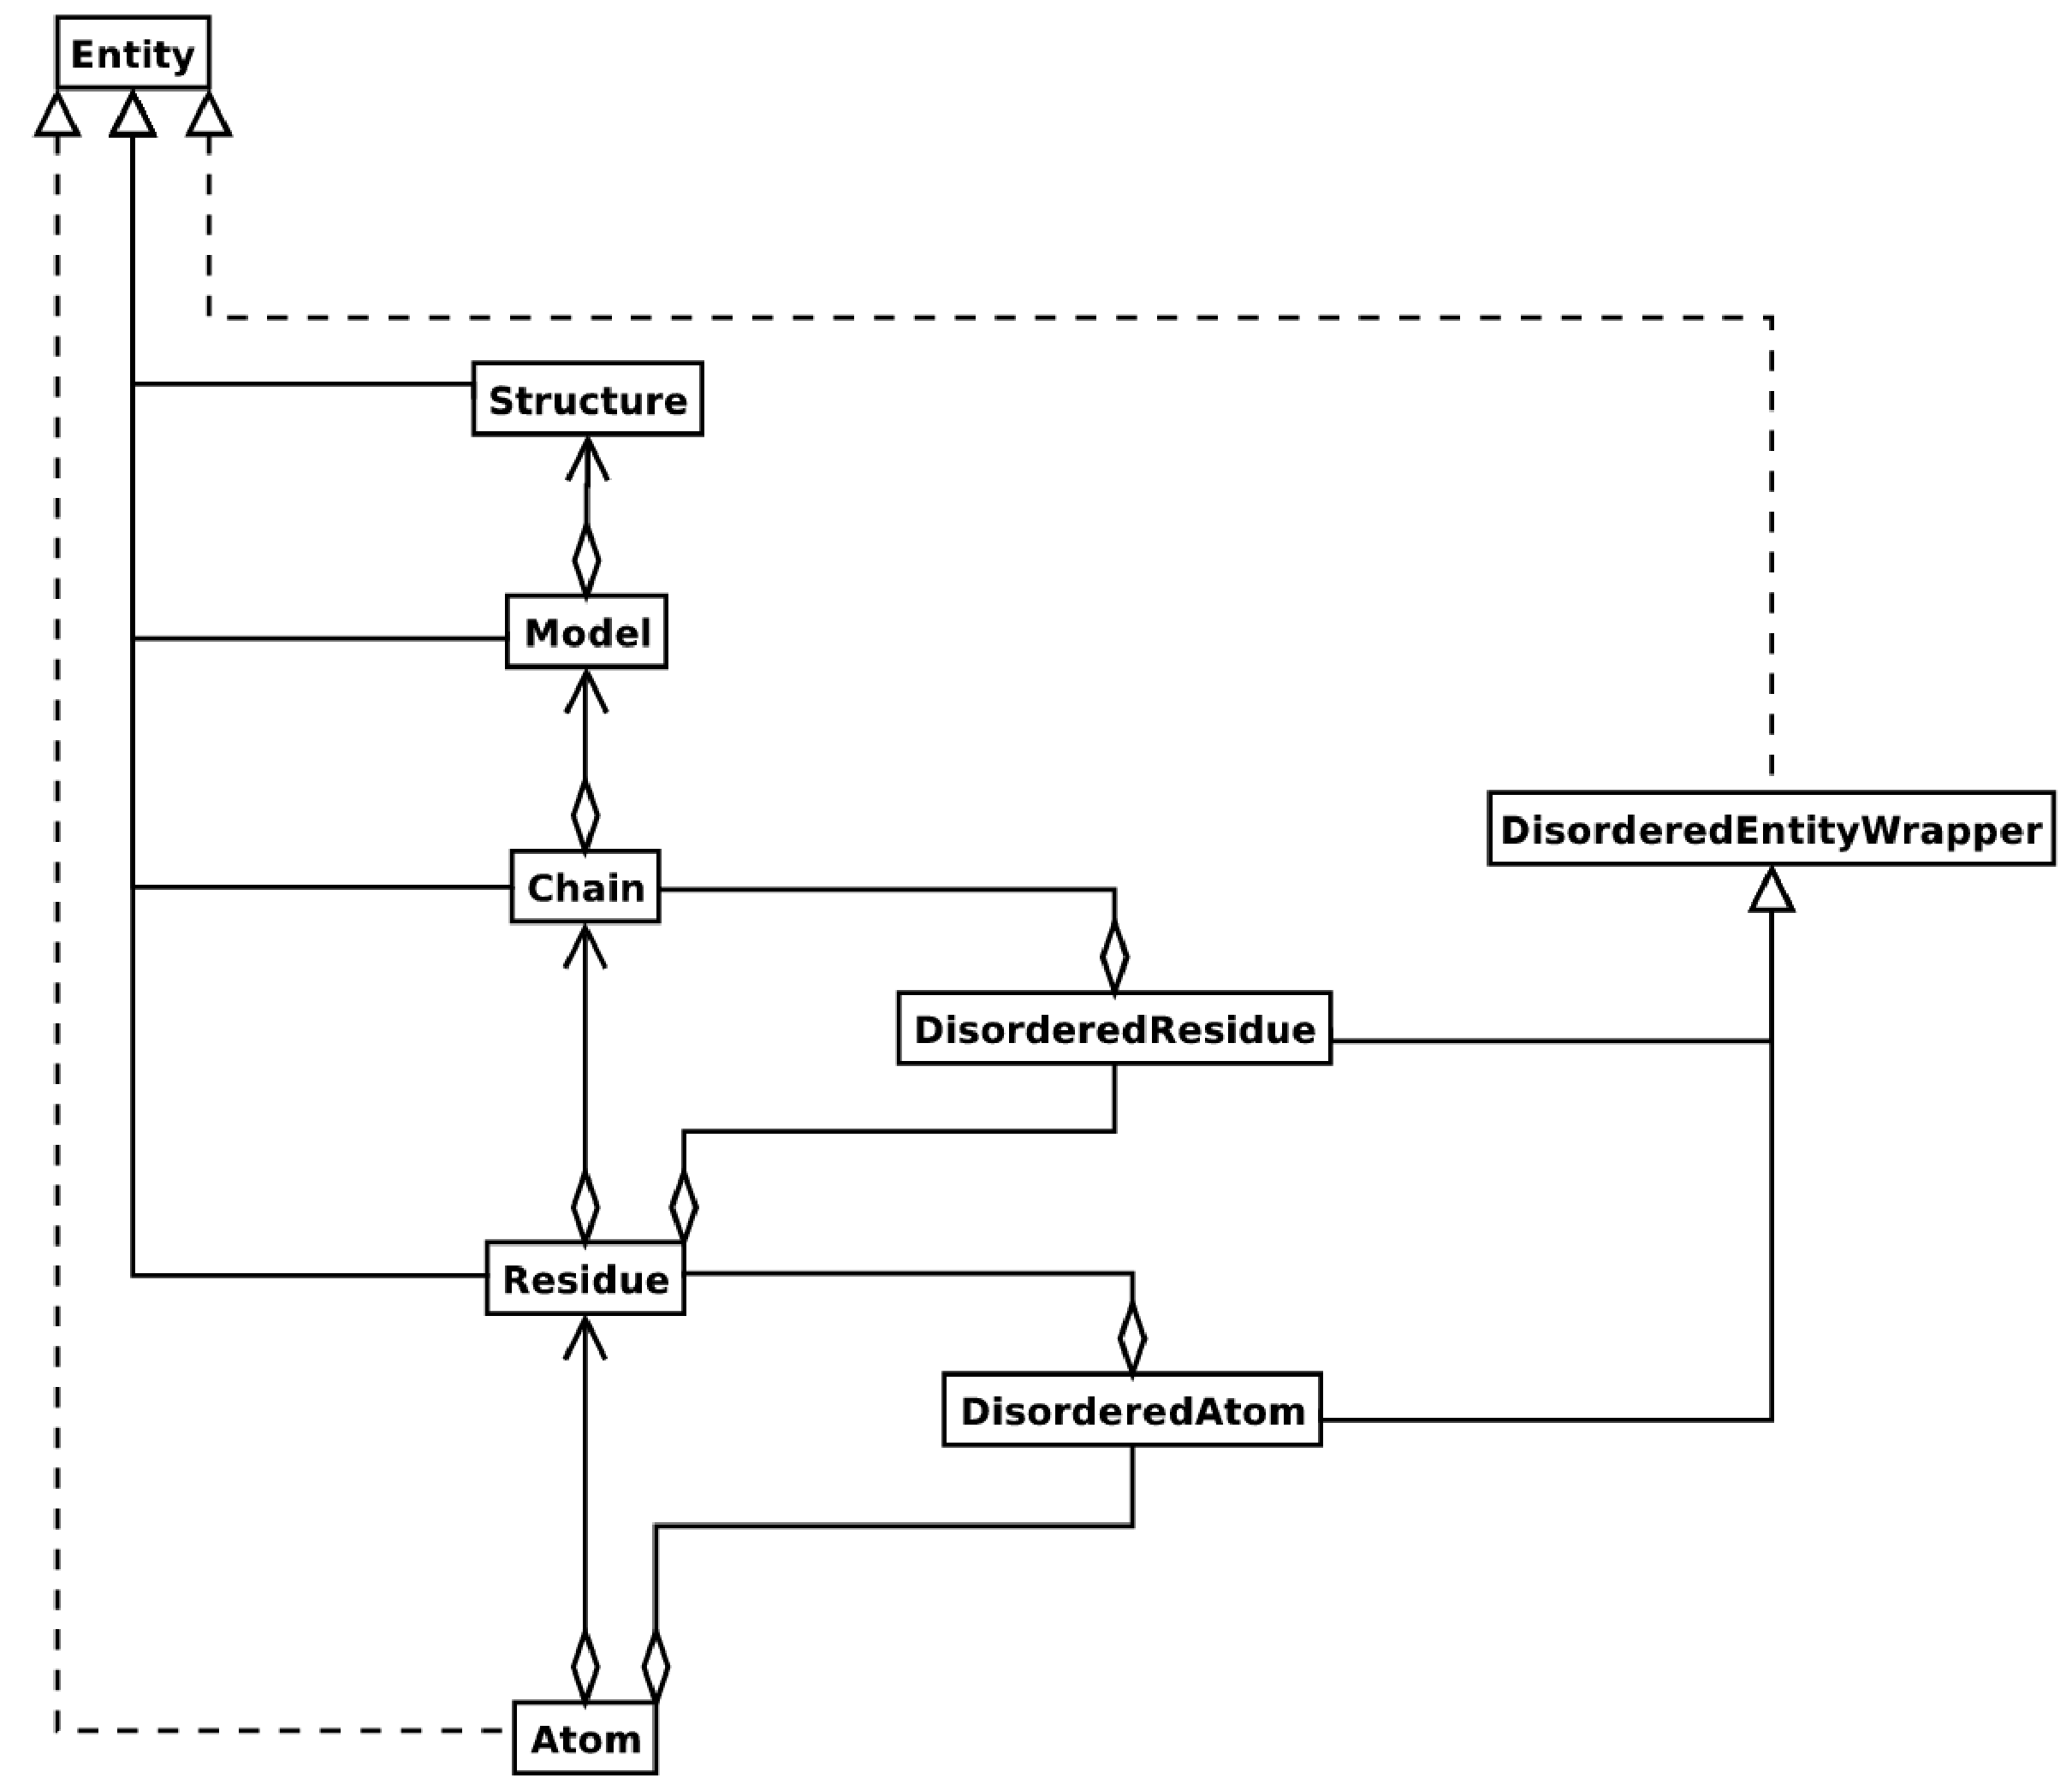
\includegraphics[width=0.8\textwidth]{images/smcra.eps}
\label{fig:smcra}
\caption{��ʬ�ҹ�¤��ɽ������ݤ˻Ȥ��� SMCRA �ǡ�����¤�� UML ���饹��}
\end{figure}

\class{Structure}��\class{Model}��\class{Chain} ����� \class{Residue}
�ϡ����������쥯�饹 \class{Entity} (����ƥ��ƥ�) �Υ��֥��饹�Ǥ���
\class{Atom} ���饹������\class{Entity} ���󥿡��ե������ΰ�������
�������Ƥ��ޤ��� (\class{Atom} ���饹�ˤϻҥ��饹��ɬ�פʤ�����Ǥ�)��

\class{Entity} ���֥��饹�Υ��֥������Ȥϡ���������դʼ��̻�
(id) �򥭡��˻Ȥ����Ȥǡ���ʬ�λҥ���ƥ��ƥ�����Ф��ޤ� (�㤨�С�
���Ҥ�̾����ɽ��ʸ����򥭡��ˤ��ơ����� \class{Residue} ���֥�������
����\class{Atom} ���֥������Ȥ���Ф����ꡤʬ�Һ��� id �򥭡���
���ơ�\class{Model} ���֥������Ȥ��� \class{Chain} ���֥������Ȥ�
���Ф�����Ǥ��ޤ�)��

���Ҥ�Ĵ�Τ�餮 (disorder) �� \class{DisorderedAtom} ��
\class{DisorderedResidue} ���饹��ɽ������ޤ��������Ϥ������
���쥯�饹\class{DisorderedEntityWrapper} �Υ��֥��饹�Ǥ���
�����Υ��饹�ϡ���餮��ȼ��ʣ�������ä��������������̤�
\class{Atom} �� \class{Residue} ���֥������ȤǤ��뤫�Τ褦�˿�����
�ޤ���

����Ū�ˤϡ�����ƥ���ƥ��ƥ� (\class{Residue}, \class{Chain},
\class{Model}, \class{Structure}) �λҤˤ����륨��ƥ��ƥ����֥�������
(\class{Atom}, \class{Residue}, \class{Model}, \class{Structure}) �ϡ�
id �򥭡��ˤ��Ƽ��Ф��ޤ���

\begin{verbatim}
child_entity=parent_entity[child_id]
\end{verbatim}

�ޤ�������ƥ���ƥ��ƥ����֥������Ȥλҥ���ƥ��ƥ����ƤΥꥹ�Ȥ�
���Ф��ޤ������Υꥹ�Ȥ��ü�ʤ�꤫�����¤�Ǥ���Τ����դ��Ƥ�����
�� (�㤨�С�\class{Model} ���֥������Ȥ��Ƥξ�硤�Ҥ�\class{Chain} 
���֥������Ȥ�¦�� id (chain identifier) �˱������¤Ӥޤ�)��

\begin{verbatim}
child_list=parent_entity.get_list()
\end{verbatim}

����ҥ���ƥ��ƥ����֥������Ȥοƥ���ƥ��ƥ����֥������Ȥ�
���Ф��ޤ���

\begin{verbatim}
parent_entity=child_entity.get_parent()
\end{verbatim}

�ޤ���SMCRA ���ؤΤɤγ��ؤΥ��֥������Ȥ��Ф��Ƥ⡤
\emph{���� id (full id)} ����Ф��ޤ���
���� id �Ȥϡ��Ǿ�̤Υ��֥������� (\class{Structure}) ���鲼�äơ�
���ߤΥ��֥������Ȥޤ�é�ä��Ȥ��˷�ͳ�������ƤΥ��֥������Ȥ� id ����
�ʤ륿�ץ�Ǥ����㤨�С����� \class{Residue} ���֥������Ȥδ��� id ��
�ʲ��Τ褦�ˤʤ�ޤ�:

\begin{verbatim}
full_id=residue.get_full_id()

print full_id

("1abc", 0, "A", ("", 10, "A"))
\end{verbatim}

���Υ��ץ�����Ƥϡ����줾��

\begin{itemize}
\item \code{"1abc"} �� id �˻��� \class{Structure} ���֥�������
\item \code{0} �� id �˻��� \class{Model} ���֥�������
\item \code{"A"} �� id �˻��� \class{Chain} ���֥�������
\item \code{("", 10, "A")} �� id �˻��� \class{Residue} ���֥�������
\end{itemize}

���б����ޤ���

�Ǹ�� \class{Residue} ���֥������Ȥ� id �ϡ��إƥ��ե������
(�ǽ�Υե������) ������ˤʤäƤ��ޤ�������ϡ����λĴ�
�إƥ��Ĵ� (�⤷���Ͽ�) �ǤϤʤ����Ȥ򼨤��Ƥ��ޤ����ޤ���
����μ��̻Ҥ� 10 �ǡ����������� (insertion code) �� \code{"A"} 
�ˤʤäƤ��ޤ���

����ƥ��ƥ��ˤϤ����Ĥ������ʥ᥽�åɤ�����ޤ�:

\begin{verbatim}
# ����ƥ��ƥ��� id ������

entity.get_id()

# ���� id ���ä��ҥ���ƥ��ƥ���¸�ߤ��뤫��Ĵ�٤�

entity.has_id(entity_id)

# �ҥ���ƥ��ƥ��ο�������

nr_children=len(entity)
\end{verbatim}

����ƥ���ƥ��ƥ����Ф��ơ����λҥ���ƥ��ƥ����������ꡤ
�ҥ���ƥ��ƥ���̾�����ѹ������ꡤ�����ʻҥ���ƥ��ƥ����ɲä������
�Ǥ��ޤ��������κݤ˥ǡ����������������å� (sanity check) ��
�Ԥ��ޤ��� (�㤨�С�����ʬ�Һ���Ʊ�� id �������ĤλĴ��
�ղä�����Ǥ��Ƥ��ޤ��ޤ�)��\class{Decorator} ���饹���Ѥ���ȡ�
��������ޤ᤿�������������å��򤦤ޤ��ԤäƤ���ޤ������⤷
�ǤΥ��󥿥ե����������Ѥ������ʤ顤������������ (\file{Entity.py})
�򻲾Ȥ��ƤߤƤ���������

\subsubsection{Structure ���֥�������}

\class{Structure} ���֥������ȤϹ�ʬ�Ҥ�ɽ������ǡ����γ��ع�¤��
ĺ���˰��֤��Ƥ��ޤ���\class{Structure} �� id �ϥ桼�������ꤷ��
ʸ����ˤʤ�ޤ���\class{Structure} ���֥������Ȥˤϡ�ʣ����
\class{Model} ���֥������Ȥ��ҥ���ƥ��ƥ��Ȥ������äƤ��ޤ���
�ۤȤ�ɤ� (���ƤǤϤ���ޤ���) �뾽��¤�ˤ�ñ��Υ�ǥ뤷��
�ʤ������� NMR �Ƿ��ꤵ��빽¤�ˤϰ���Ū�ˤ����Ĥ��Υ�ǥ뤬
���äƤ��ޤ����뾽��¤�ˤ�����¿����ʬ�Ҥˤ�餮�������Ƥ�����
�ˤ⡤ʣ���Υ�ǥ뤬�Ǥ��ޤ���

\paragraph{Structure ���֥������Ȥ��ۤ���}

\class{Structure} ���֥������Ȥ� \class{PDBParser} ���֥������Ȥ���
��������ޤ�:

\begin{verbatim}
from Bio.PDB.PDBParser import PDBParser

p=PDBParser(PERMISSIVE=1)

structure_id="1fat"

filename="pdb1fat.ent"

s=p.get_structure(structure_id, filename)
\end{verbatim}

\var{PERMISSIVE} �ե饰�ϡ�PDB �ե�����˴ؤ���褯���뤤���Ĥ�������
(\ref{problem structures} ����) ��ѡ�����̵�뤵���ޤ� (�ȤϤ�����
����ˤ�äƤ����Ĥ��θ��Ҥ�Ĵ𤬼����뤫�⤷��ʤ��Τ����դ���
��������) �����Τ��Υե饰����ꤷ�ʤ���硤�ѡ����� PDB �ե������
��ʸ���Ϥ��Ƥ���ݤ����꤬�������\exception{PDBConstructionException}
�����Ф��ޤ���

\paragraph{�إå� (header) �ȥȥ쥤�� (trailer)}

\function{get_header} ����� \function{get_trailer} �Ȥ��ä��᥽�åɤ�
�Ѥ���ȡ�PDB �ե�������Υإå��ȥȥ쥤��� (ʸ���󤫤�ʤ�ñ��ʥꥹ��
��) \class{PDBParser} ���֥������Ȥ�����Ф��ޤ���

\subsubsection{Model ���֥�������}

\class{Model} ���֥������Ȥ� id �������ǡ�PDB �ե��������Ϥ����ݤ�
���Υ�ǥ뤬���֤��Ƥ�����꤫���ޤ�ޤ� (0 ���鼫ưŪ���ֹ��դ�
����ޤ�)��\class{Model} ���֥������Ȥˤϡ��ҥ���ƥ��ƥ���\class{Chain} 
����ʤ�ꥹ�Ȥ����äƤ��ޤ���


\paragraph{����}

\class{Structure} ���֥���������˼�����Ƥ���ǽ��
��ǥ��������ޤ���

\begin{verbatim}
first_model=structure[0]
\end{verbatim}

\subsubsection{Chain ���֥�������}

\class{Chain} ���֥������Ȥ� id �ϡ���¤�ǡ������ҥե��������
��������ʬ�Һ���ɽ����ʬ�μ��̻Ҥ���Ȥ�졤���餫��ʸ����ˤʤ�ޤ���
����\class{Model} ���֥������Ȳ��ˤ���ơ���\class{Chain} �ˤ�
�ߤ��˰�դ� id ������ޤ���\class{Chain} ���֥������Ȥˤ�
�ҥ���ƥ��ƥ���\class{Residue} ����ʤ�ꥹ�Ȥ����äƤ��ޤ���

\paragraph{����}

\class{Model} ���֥������Ȥ��顤���̻� \code{"A"} ���ä�
\class{Chain} ���֥������Ȥ�������ޤ���

\begin{verbatim}
chain_A=model["A"]
\end{verbatim}

\subsubsection{Residue ���֥�������}

�����ޤǤ�ʤ���\class{Residue} �ϰ�Ϣ��\class{Atom} ��ҥ���ƥ��ƥ�
�Ȥ��Ƶ������Ƥ��ޤ�������˲ä��ơ�\class{Residue} �ˤϻĴ��̾��
�򼨤�ʸ���� (�㤨�� \code{"ASN"}) �ȡ��Ĵ�Υ������ȼ��̻�
(X-PLOR �桼���ˤϤ褯�Τ��Ƥ��ޤ�����SMCRA �ǡ�����¤���ۤ���
�ݤˤ��Ѥ����ޤ���) �����äƤ��ޤ���

\class{Residue} ���֥������Ȥ� id �ϻ��Ĥ���ʬ: �إƥ��ե������
(hetfield)�������̻� (resseq)������������ (icode) ����ʤ�ޤ���

�إƥ��ե�����ɤ�ʸ����ǡ�\code{"W"} �Ͽ��\code{"H_"} �θ����
�Ĵ�̾��³������� (�㤨�� \code{"H_FUC"}) �Ϥ���¾�Υإƥ��Ĵ��
����ϰ���Ū�ʥ��ߥλ��ȳ˻���ɽ���ޤ���������ˡ����Ѥ�����ͳ��
\ref{hetero problems} ��Dz��⤷�Ƥ��ޤ���

�Ĵ� id ������Υե�����ɤ������̻Ҥǡ�ʬ�Һ���
�ɤξ��˻Ĵ𤬷�礷�Ƥ��뤫��ɽ���ޤ���

�軰�Υե�����ɤ�ʸ����ǡ����������ɤ�����ޤ������������ɤ�
���Ф��С�����λĴ���Ф���˾�ޤ������ֹ��դ���ˡ����¸���뤿���
�Ȥ��ޤ���Ser 80 �����ߥ塼����� (�㤨�С�Thr 80 �� Asn81 �Ĵ��
�֤� Ser �����ä����) �ξ�硤�����̻Ҥ����������ɤϤ��줾��
Thr 80 A, Ser 80 B, Asn 81 �Τ褦�ˤʤ�ޤ���������ˡ��Ȥ�ȡ�
�Ĵ���ֹ��դ���ˡ���������ι�����Ʊ���ޤޤˤʤ�ޤ���

�����Ĥ����󤲤Ƥߤޤ��礦�� ���������ɤ�����ˤʤäƤ��� Asn 10 
�λĴ� id ��\code{("", 10, "")} �Ǥ���W 10 �λĴ� id ��
\code{("W", 10, "")} �Ǥ��������̻� 10 �Υ��륳����ʬ�� (�إƥ�
�Ĵ� GLC �Ȥ���̾���ˤʤäƤ��ޤ�) �� \code{("H_GLC", 10, "")}
�Ǥ������Τ褦�ˤ���ȡ����ƤλĴ�ϰۤʤ�Ĵ� id ����ĤΤǡ�
Ʊ��ʬ�Һ��ΰ���ʬ�Ȥ��ư����ޤ���

�ۤȤ�ɤξ�硤 \member{hetflag} �� \member{icode} �ե�����ɤ϶���
���ʤ��\code{("W", 10, "")} �Τ褦�ˤʤ�ޤ������Τ褦�ʾ��ˤϡ�
�����̻Ҥϴ��� id �Υ��硼�ȥ��åȤȤ������ѤǤ��ޤ�:

\begin{verbatim}
# ���� id ���

res10=chain[("", 10, "")]

# ���硼�ȥ��åȤλ��� 

res10=chain[10]
\end{verbatim}

\class{Chain} ���֥������Ⱦ�γ� \class{Residue} ���֥������Ȥˤ�
��դ� id ���Ĥ����Ƥ��ޤ����Ĵ�Τ�餮�����̰�������ޤ���
����ˤĤ��Ƥ�\ref{point mutations} ����������ޤ���

\class{Residue} ���֥������Ȥˤϡ�¾�ˤ⤤���Ĥ��᥽�åɤ�����ޤ�:

\begin{verbatim}
r.get_resname()         # "ASN" �Τ褦�ʻĴ�̾���֤�
r.get_segid()           # "CHN1" �Τ褦�� SEGID ���֤�
\end{verbatim}

\subsubsection{Atom}

\class{Atom} �ϸ��Ҥ˴�Ϣ����ǡ����򵭲������ҥ���ƥ��ƥ�������ޤ���
���Ҥ� id �Ϥ��θ��Ҥ�̾���ˤʤ�ޤ� (�㤨�С�\code{"OG"} �� Ser �Ĵ��
¦���λ��ǤǤ�)������Ĵ���Ǥϡ��ġ��θ��Ҥ� id �ϰ�դǤʤ����
�ʤ�ޤ���\ref{disordered atoms} ��Ǥ�Ҥ٤��褦�ˡ��ǡ�����ʸ����
����ݤ˸��ҤΤ�餮������������㳰��ȯ�����ޤ���

PDB �ե�������Ǥϡ����Ҥ�̾���� 4 ʸ���Υ���饯������ʤꡤ�̾��
��Ƭ�������˶��򤬤Ĥ��Ƥ��ޤ���PDB �ե�����Ǥϡ���ñ�Τ����
���Ф��Ф��ζ���Ͻ����ޤ� (�㤨�С����ߥλ�C$\alpha$ ��
PDB �ե�������Ǥ� \code{".CA."} �ǡ��ɥåȤ������ɽ���ޤ�)��
����Ĵ����̾���ξ��� (Ʊ��̾���� id ����� \class{Atom} ���֥�������
�����������) ��������ʤ��¤ꡤ���Ҥ�̾������������ݤ˥��ڡ�����
����ޤ������ͤ�ȯ�������硤�ѡ����ϥ��ڡ�����ޤ᤿����̾��Ȥ�����
��ߤޤ������Τ褦�ʾ����ϡ��㤨�а�ĤλĴ�� \code{".CA."} ��
\code{"CA.."} �Ȥ���̾���θ��Ҥ����äƤ������ȯ�����ޤ�����
��ä��˵����뤳�ȤϤ���ޤ���

�Ĵ����¸����Ƥ��븶�ҤΥǡ����ˤϡ����Ҥ�̾�������Ҥκ�ɸ
(�⤷�����ɸ���к���)��B �ե����� (�⤷����а����� B �ե�������
ɸ���к���)�� altloc ����Ҥȶ����ޤര���ʸ���̾�����äƤ��ޤ���
�����ֹ� (element number) �丶�Ҥ��Ų٤Ȥ��ä������ޤ����Ѥ���ʤ�
���Ǥϡ� PDB �ե�������ˤϽ񤫤�Ƥ��ޤ���\class{Atom} �Υǡ�����
���Ƥ���¸����ޤ���

\class{Atom} ���֥������Ȥˤϰʲ��Τ褦�ʥ᥽�åɤ�����ޤ�: 

\begin{verbatim}
a.get_name()       # ����̾ (���ڡ����ʤ����㤨�� "CA")

a.get_id()         # id (����̾��Ʊ��)

a.get_coord()      # ���Һ�ɸ

a.get_bfactor()    # B �ե�����

a.get_occupancy()  # ���Ҥ�餮�ˤ�������ͭΨ

a.get_altloc()     # _REPLACE_���ع�¤�������ֻ���� (alternative location specifier) 

a.get_sigatm()     # ���ҥѥ�᥿��ɸ���к�

a.get_siguij()     # ������ B �ե�������ɸ���к�

a.get_anisou()     # ������ B �ե�����

a.get_fullname()   # ����̾ (���ڡ�����ޤ�, ��. ".CA.")
\end{verbatim}

���Ҥκ�ɸ�������� B �ե���������Ӥ���ɸ���к���
���ҥѥ�᥿��ɸ���к���ɽ���ˤ� Numerical Python ������
�Ѥ����Ƥ��ޤ���

\subsection{��餮 (disorder)}


\subsubsection{����Ū�ʥ��ץ�����}
\label{disorder problems}

ʬ�ҹ�¤�Τ�餮 (disorder) ��ͤ���ˤϡ���Ĥλ���������ޤ���
��Ĥϸ��ҤΤ�餮���⤦��ĤϻĴ�Τ�餮�Ǥ��������Ƥ����桹��
��餮���餯��ʣ���������ƥ��ץ��벽���ư������Ȥ��Ƥ��ޤ��ޤ���
���������⤷����ñ�����Ƥ� C$\alpha$ ���Ҥˤ錄�äƥ롼�׽�����
�Ԥ����������ʤ顤�ɤ����λĴ��¦���ˤ�餮�����äƤⵤ�ˤ�
���ޤ��󡥤��ΰ����ǡ��ǡ�����¤��Ǥϡ���餮������ɽ��
�Ǥ��ʤ���Фʤ�ʤ��Ȥ������꤬����ޤ��������ǡ����Ҥ�Ĵ��
��餮���ü�ʥ��֥������Ȥ����졤���������餮��¸�ߤ��ʤ�����
�褦�˿���碌�뤳�Ȥˤ��ޤ�����������������Ԥ�ͣ�����ˡ�ϡ�
��餮����ĸ��Ҥ�Ĵ�Υ��֥��åȤˤ��ɽ���Ǥ����ɤΥ��֥��åȤ�
���Ѥ��뤫 (�㤨�С�Ser �Ĵ𤬻Ȥ��Ƥ�����ǡ����̤�ˤ�餮��
���� OG ¦���Τɤ�������֤�) �ϡ��桼��������Ǥ��ޤ���


\subsubsection{���ҤΤ�餮}
\label{disordered atoms}

���ҤΤ�餮�ξ�硤��餮�Τ�����ʬ�θ��Ҥ��̾��\class{Atom} 
���֥������Ȥ�Ȥä�ɽ�����ޤ��������������θ��Ҥ�ʪ��Ū��Ʊ��
���Ҥ�ɽ�����Ƥ���褦�ʸ��Ҥϡ����� \class{DisorderedAtom} 
���֥������������¸���ޤ���\class{DisorderedAtom} ���֥����������
��\class{Atom} ���֥������Ȥϡ�\member{altloc} ����Ҥ�Ȥäư�դ�
����Ǥ��ޤ���
\class{DisorderedAtom} ���Ф��ƥ᥽�åɸƤӽФ���Ԥ��ȡ�
\class{DisorderedAtom} �ǽ�������ʤ���Τϸ������򤵤�Ƥ���
\class{Atom} ���֥������Ȥ�ž�����ޤ����ǥե���ȤǤϡ�
��ͭΨ (occupancy) �κǤ�⤤\class{Atom} ���֥������Ȥ����򤵤��
���ޤ����������\member{altloc} �����Ѥ���С��桼���Ϥ����줫��
\class{Atom} ���֥������Ȥ�����Ǥ��ޤ������Τ褦�ˤ��ơ�������ʣ����
���������Ȥʤ������Ҥ�餮��������ɽ���Ǥ���褦�ˤʤäƤ���ΤǤ���
�̤θ������򤹤�С����Ҥ�餮�˶�̣���ʤ���С�����ˤ鷺��蘆���
ɬ�פϤʤ��Ȥ������ȤǤ���

��餮�θ��Ҥˤϡ����줾�� \member{altloc} �Ȥ������̻Ҥ�����ޤ���
\class{DisorderedAtom} ���֥������Ȥˤ��μ��̻Ҥ���ꤹ��ȡ�
����� \member{altloc} ���̻Ҥ���ä� \class{Atom} �Ǥ��뤫�Τ褦��
����碌���ޤ�:

\begin{verbatim}
atom.disordered_select("A")        # altloc �� A �θ��Ҥ����򤹤�
print atom.get_altloc()
"A"

atom.disordered_select("B")        # altloc �� B �θ��Ҥ����򤹤�
print atom.get_altloc()
"B"
\end{verbatim}

\subsubsection{�Ĵ�Τ�餮}

\paragraph{�褯���륱����}

��äȤ�褯����Τϡ��Ĵ�˰�Ĥޤ��Ϥ���ʾ�θ��ҤΤ�餮��
���륱�����Ǥ��������ޤǤ�ʤ������Υ�������\class{DisorderedAtom} 
���֥������Ȥˤ�äƤ�餮�Τ��븶�Ҥ�ɽ����������
\class{DisorderedAtom} ���֥������Ȥ�\class{Residue} ���֥������Ȥ�
������̤�\class{Atom} ���֥������ȤΤ褦�ˤ��������в�褷�ޤ���
\class{DisorderedAtom} �ϡ���ʬ��Ŭ�Ѥ��줿�᥽�åɤΤ�����
\class{DisorderedAtom} �ǽ�������ʤ���Τ�������\class{Atom} 
���֥������� (���򤵤�Ƥ��� \class{Atom} ���֥�������) 
��ž�����뤳�Ȥǡ����������̾�θ��ҤȤޤä���Ʊ���褦�� 
(�ºݤˤϺǤ���ͭΨ�ι⤤���Ҥ�Ʊ���褦��) �����񤤤ޤ���

\paragraph{���Ѱ�}
\label{point mutations}
��餮�����Ѱ� (point mutation) ��ͳ�褹��褦���ü�ʥ�������
�㤨�����Ѱ��Τ���İʾ庮���ä��ݥ�ڥץ��ɤ��뾽��˸��Ĥ���褦��
��礬����ޤ������Τ褦����ΰ�Ĥ� PDB ��¤�� 1EN2 �Ǥ���

���������ѰۤǤϡ��Ĵ� (�㤨�� Ser 60 �� Cys 60 �Τ褦��) �ۤʤ�
�Ĵ𷿤�°����Τǡ���Τ褯������Τ褦�ˡ���Ĥ� \class{Residue}
���֥������Ȥ���ˤ�����ޤ��󡥤��Τ褦�ʥ������Ǥϡ�
��餮�Ȥʤ�ơ��λĴ��\class{Residue} ���֥������Ȥ�ɽ�����Ƥ�����
ξ���� \class{Residue} ���֥������Ȥ� \class{DisorderedResidue}
���֥������Ȥ�����Ƥ����ޤ��� 

\class{DisorderedResidue} �ϡ���ʬ��Ŭ�Ѥ��줿�᥽�åɤΤ�����
\class{DisorderedResidue} �ǽ�������ʤ���Τ򸽺����򤵤��
����\class{Residue} ���֥������� (�ǥե���ȤǤϺǸ���ɲ�
���줿\class{Residue} ���֥�������) ��ž�����뤳�Ȥǡ�
���������̾�λĴ�Τ褦�˿��񤤤ޤ���\class{DisorderedResidue} 
���֥���������γ�\class{Residue} ���֥������Ȥϡ��ơ���
�Ĵ�̾�ǰ�դ˼��̤Ǥ��ޤ��������Ǥ����С� 
\class{DisorderedResidue} ���֥���������� Ser 60 �Ĵ��
���̻Ҥ�\code{"SER"} ��Cys 60 �μ��̻Ҥ�\code{"CYS"} �Ǥ���
�桼���Ϥ��μ��� id ��ȤäƸ���ͭ���� \class{Residue} ���֥�������
������Ǥ��ޤ���

\subsection{�إƥ��Ĵ�}

\subsubsection{�إƥ��Ĵ�˴�Ϣ��������}
\label{hetero problems}

�إƥ��Ĵ�˴ؤ��Ƥ褯��������ϡ������Ĥ��Υإƥ��Ĵ����إƥ��Ĵ��Ʊ��
����������Ʊ��������̻�(����������������)��ͭ���뤳�ȤǤ��롣��
�Τ��ᡢ�Ƥإƥ��Ĵ���ȼ���id���������뤿���Ȥ���¾�Υإƥ��Ĵ�ϰ�
�ʤ���ˡ�ǰ����롣

�إƥ��Ĵ�˴ؤ��Ƥ褯��������ϡ�Ʊ��ʬ�Һ���ˤ���ʣ���Υإƥ��Ĵ�
��إƥ��Ĵ𤬡�Ʊ�������̻�(���������������) ����äƤ����
�������ȤǤ����������äơ��ƥإƥ��Ĵ�� id ���դ��������뤿��ˡ�
��䤽��¾�Υإƥ��Ĵ���̤���ˡ�ǰ����ޤ���

\class{Residue} ���֥������Ȥ� \code{(hetfield, resseq, icode)} �Ȥ���
���ץ�� id ����äƤ��뤳�Ȥ�פ��Ф��Ƥ������������ߥλ���˻���
��硤 \member{hetfield} �϶� (\code{""}) �ˤʤꡤ���إƥ��Ĵ�ξ��ˤ�
ʸ����ˤʤ�ޤ���\member{hetfield} �����ƤˤĤ��Ƥϡ��ʲ����������ޤ���

\subsubsection{��Ĵ�}

��Ĵ�� \member{hetfield} ��ʸ����� \code{"W"} �ˤʤ�ޤ������Τ��ᡤ
��ΰ���Ū��id�� \code{("W", 1, "")} �Ǥ���

\subsubsection{����¾�Υإƥ��Ĵ�}

����¾�Υإƥ��Ĵ�� \member{hetfield} ʸ����ϡ�\code{"H_"} �˻Ĵ�̾��
³������ΤǤ����㤨�С��Ĵ�̾ \code{"GLC"} �Υ��륳����ʬ�Ҥξ�硤
\member{hetfield} �� \code{"H_GLC"} �ˤʤ�ޤ����Ĵ� id �� 
\code{("H_GLC", 1, "")} �Ǥ���

\subsection{������}

PDB�ե��������Ϥ��ơ�\class{Model}��\class{Chain}�� \class{Residue}
����ӡ�\class{Atom} ���֥������Ȥ���Ф��ޤ���

\begin{verbatim}
from PDBParser import PDBParser 

parser=PDBParser()

structure=parser.get_structure("test", "1fat.pdb")
model=structure[0]
chain=model["A"]
residue=chain[1]
atom=residue["CA"]
\end{verbatim}

ʬ�Һ�����إƥ��Ĵ� (�����Ǥϰ����� resseq 10 �Υ��륳���� (GLC) 
�Ǥ���褦�ʻĴ�) ����Ф��ޤ���

\begin{verbatim}
residue_id=("H_GLC", 10, " ")
residue=chain[residue_id]
\end{verbatim}

ʬ�Һ�������ƤΥإƥ��Ĵ����Ϥ��ޤ���

\begin{verbatim}
for residue in chain.get_list():
	residue_id=residue.get_id()
	hetfield=residue_id[0]
	if hetfield[0]=="H":
		print residue_id
\end{verbatim}

B �ե������� 50 �ʾ�� CA ���Ҥκ�ɸ�����ƽ��Ϥ��ޤ���

\begin{verbatim}
for model in structure.get_list():
  for chain in model.get_list():
    for residue in chain.get_list():
      if residue.has_id("CA"):
        ca=residue["CA"]
        if ca.get_bfactor()>50.0:
          print ca.get_coord()
\end{verbatim}

��餮�Τ��븶�Ҥ�ޤ����ƤλĴ����Ϥ��ޤ���

\begin{verbatim}
for model in structure.get_list()
  for chain in model.get_list():
    for residue in chain.get_list():
      if residue.is_disordered():
        resseq=residue.get_id()[1]
        resname=residue.get_resname()
        model_id=model.get_id()
        chain_id=chain.get_id()
        print model_id, chain_id, resname, resseq
\end{verbatim}

��餮�Τ��븶�����Ƥˤ錄�äƥ롼�פ��ơ����� \member{altloc} �� 
\code{"A"} �θ��� (�������) �ˤʤ�褦���򤷤ޤ�����������Ԥ��ȡ�
SMCRA �ǡ�����¤�ε�ư�� \member{altloc} �� \code{"A"} �θ��Ҥ���
¸�ߤ��ʤ����ε�ư�ˤ��ޤ���

\begin{verbatim}
for model in structure.get_list()
  for chain in model.get_list():
    for residue in chain.get_list():
      if residue.is_disordered():
        for atom in residue.get_list():
          if atom.is_disordered():
            if atom.disordered_has_id("A"):
              atom.disordered_select("A")
\end{verbatim}

ʬ�Һ��ΰ��� 10 �����Ѱۤ����äơ� Ser �� Cys ����ʤ�Ȥ��ޤ���
ʬ�Һ��ε�ư����� 10 �λĴ� Cys �Ĵ�Ǥ�����ε�ư�ˤ��ޤ���

\begin{verbatim}
residue=chain[10]
residue.disordered_select("CYS")
\end{verbatim}

\subsection{PDB �ե�����ˤ褯��������}
\subsubsection{��}
\label{problem structures}
\class{PDBParser}/\class{Structure} ���饹�ϡ�
(�ơ� SCOP �ǰۤʤ� �����ѡ��ե��ߥ꡼��°���Ƥ���) �� 800 ��
����ѥ���¤�ǥƥ��Ȥ�Ԥ��ޤ����������ˤ��� 20 ʬ���פ���
�칽¤�������ʿ�Ѥ� 1.5 �äǤ����� 64000 ���Ҥ�ޤ��ܥ������
�祵�֥�˥å� (1FKK) �Υǡ�����¤���Ϥˤϡ� 1000 MHz �� PC ���
10 �ä�����ޤ�����

���Υƥ��Ȥ���ǡ������ޤ��Ǥʤ��ǡ�����¤���ۤǤ��ʤ��Ȥ�����ͳ��
�㳰�� 3 �����Ф���ޤ�����������Υ������ˤ����Ƥ⡤���顼�θ�����
PDB �ե�����¦�ǽ������٤�����Ǥ��������������������Ǥϡ��㳰��
���Ф����������ǡ�����¤�˽񤫤�Ƥ������Ƥ���ä�ɽ�����Ƥ��ޤ�
����Ϥ뤫�ˤޤ��Ǥ���

\paragraph{�Ĵ�ν�ʣ (duplicate residues)}

���빽¤�Ǥϡ���Ĥ�ʬ�Һ������ĤΥ��ߥλ��Ĵ�Ʊ�������̻�
(resseq 3) �� icode ����äƤ��ޤ�����Ĵ�٤��Ȥ�����
����ʬ�Һ��� Thr A3, \ldots{}, Gly A202, Leu A3, Glu A204 �Τ褦��
�ʤäƤ��ޤ�����Leu A3 ���������� A203 �ʤΤ����餫�Ǥ���
Ʊ���褦�ʾ����� 1FFK �ˤ⤢��ޤ��� (Gly B64, Met B65, Glu B65, 
Thr B67, �ĤޤꡤGlu B65 �� Glu B66 �θ���)��


\paragraph{���Ҥν�ʣ (duplicate atoms)}

ʬ�ҹ�¤ 1EJG �ϡ�ʬ�Һ� A �� 22 ���ܤλĴ� Ser/Pro �����Ѱۤ�
�ʤäƤ��ޤ�������ˡ� Ser 22 �Τ����Ĥ��θ��ҤϤ�餮����äƤ��ޤ���
�������̤ꡤSer22 ��°�������Ƥθ��Ҥˤ϶���Ǥʤ� \member{altloc}
����� (B �ޤ��� C) �����ꡤPro 22 �����Ƥθ��Ҥ� \member{altloc} A
�Ǥ��������������� N �� \member{altloc} ����������ˤʤäƤ��ޤ�����
���줬�㳰�����Ф��븶���ˤʤäƤ��ޤ������Ȥ����Τ⡤���Ѱۤ�
�����Ƥ�����Ǥϡ������λĴ�������äƤ������Ƥθ��Ҥ˶���Ǥʤ�
\member{altloc} ���Ĥ��Ƥ��ʤ���Фʤ�ʤ�����Ǥ���Ser 22 �ˤ�
���� N ���ʤ��ä��Τǡ������餯���θ��Ҥ� Ser 22 �� Pro 22 �δ֤�
��ͭ����Ƥ���Τ������Ȥ������Ȥ�狼��ޤ��������ޤ���
�ե�����ˤ�����������󵯤��Ƥ��ޤ�: ���� N �� Ser �� Pro �Ĵ��
ξ���ˤʤ��ƤϤʤ餺������Ŭ�ڤ� \member{altloc} ���̻Ҥ��Ϣ�դ���
���ʤ���Фʤ�ʤ��ΤǤ���


\subsubsection{��ư����}

���顼�Τ����Ĥ��Ϥ��ʤ�褯�����Τǡ����ä�����Ԥ��ꥹ����
�������������˴�ñ�˽����Ǥ��ޤ������Τ褦�ʾ���ʲ��˼����ޤ���

\paragraph{����� altloc ��ȼ�����Ҥ�餮}

�̾��餮�θ��Ҥ� \member{altloc} ���̻Ҥ϶���Ǥ��äƤϤʤ�ޤ���
�����������λ��ͤ˽��鷺��\member{altloc} ������Τ�ΤȤ����Ǥʤ���Τ�
�ȤäƤҤȤĤθ��ҤΤ�餮��ɽ�����Ƥ����Τ�����ޤ������Τ褦��
��餮��ɽ�������äƤ⡤��ưŪ����������ˡ�Dz�ᤵ��ޤ���

\paragraph{��»���Ƥ���ʬ�Һ�}

���ˡ�ʬ�Һ� A ��°���Ƥ��뤢��Ĵ�θ����ʬ�Һ� B ��°����Ĵ�
³��������ˤ��θ����ʬ�Һ� A ��°����Ĵ𤬽и�����褦�ʻĴ���
ʬ�ҹ�¤������äƤ����硤���ʤ��ʬ�Һ�������»���Ƥ���׾�礬
����ޤ������Τ褦�ʻĴ��󤬤��äƤ⡤�����������Ԥ��ޤ���

\subsubsection{��̿Ū�ʥ��顼}

���ˡ�PDB �ե������ۣ�椵�ʤ��˲��Ǥ��ʤ���礬����ޤ������ξ�硢
���ƿ��̤�ְ㤤�Υꥹ������������Ϥ������㳰�����Ф��ơ��桼����
PDB �ե��������������褦¥���ޤ����ʲ��ˤ��Τ褦�ʥ������򼨤��ޤ���

\paragraph{�Ĵ�ν�ʣ}

����ʬ�Һ�������ƤλĴ�ˤϰ�դ� id ������ޤ������� id �ϡ�
\begin{itemize}
\item �����̻� (resseq) 
\item ���������� (icode) 
\item \member{hetfield} ʸ���� (��� \code{"W"}������¾�Υإƥ��Ĵ��
\code{"H_"} �θ���˻Ĵ�̾��³�������)
\item ���Ѱۤξ��ˤϳƻĴ�λĴ�̾ (\class{DisorderedResidue} 
���֥�������������äƤ��� \class{Residue} ���֥������Ȥξ����
����뤿��)
\end{itemize}
�˴�Ť�����������Ƥ��ޤ���
�⤷���δ��ǰ�դ� id �������Ǥ��ʤ���С��ʤˤ��ޤ������Ȥ������Ƥ���
�Ϥ��ʤΤǡ��㳰�����Ф��ޤ���


\paragraph{���Ҥν�ʣ}

����Ĵ�������Ƥθ��Ҥˤϰ�դ� id ������ޤ������� id �ϡ�
\begin{itemize}
\item ����̾ (���ڡ����ʤ������������꤬��������ϥ��ڡ�����ޤ�)
\item \member{altloc} ����� 
\end{itemize}
�˴�Ť�����������Ƥ��ޤ���

�⤷���δ��ǰ�դ� id �������Ǥ��ʤ���С��ʤˤ��ޤ������Ȥ������Ƥ���
�Ϥ��ʤΤǡ��㳰�����Ф��ޤ���


\subsection{����¾�ε�ǽ}
�뾽��¤����Ϥ��뤿��Υġ����¾�ˤ⤤���Ĥ�����ޤ�����������
�ġ���Ǥϡ�2 �Ĥκ�ɸ���åȤ�Ť͹�碌 (SVDSuperimposer) ���ꡢ
��¤����ݥ�ڥץ��ɤ���Ф���ġ��� (Polypeptide) ���ꡢ
���������Τ�õ���� (NeighborSearch) ���ꡤ PDB �ե������񤭽Ф�
(PDBIO) ����Ǥ��ޤ���
�������ѥ�����õ���ˤ� \Cpp �ǽ񤫤줿 KD �ڥ⥸�塼���ȤäƤ��ޤ���
���Υ⥸�塼��ϤȤƤ��®��ư����ߤ�������ε�Υ��ˤ���褦�����Ƥ�
��ɸ�����Ф�õ�������®�ʼ�ˡ�����äƤ��ޤ���

\class{Polypeptide} ���֥������Ȥ�ñ�� \class{Residue} ���֥������Ȥ���
�ʤ�\class{UserList} �˲᤮�ޤ���\class{Structure} ���֥������Ȥ���
\class{Polypeptide} ���֥������ȤΥꥹ�Ȥ��ۤ���ˤϰʲ��Τ褦��
���ޤ�:

\begin{verbatim}
model_nr=1
polypeptide_list=build_peptides(structure, model_nr)

for polypeptide in polypeptide_list:
    print polypeptide
\end{verbatim}

\class{Polypeptide} ���֥������ȤϾ��ñ���\class{Model} (���ξ��Ǥ�
1 ���ܤΥ�ǥ�) ������������ޤ���

\section{����¾}

\subsection{DNA ���󤫤饿��ѥ�����ؤ�����}

 % draft
\chapter{���Ը���������}

\section{���󥯥饹}

\section{�󵢥ƥ��ȥե졼����}
\label{sec:regr-test}

Biopython �ˤϲ󵢥ƥ��ȥե졼����������ޤ������Υե졼������
��Ȥ�� Andrew Dalke �ˤ�äƽ񤫤졤���θ� Brad Chapman �ˤ�ä�
PyUnit �١����˰ܿ�����ޤ������󵢥ƥ��Ȥϡ������ɤ������������
��ǽ�ʸ¤�Х���ʤ��������Ω�äƤ��ޤ���

\subsection{�󵢥ƥ��Ȥ��}

Biopython �������⥸�塼��ˤϡ����ƥƥ��Ȥ� (�����ƥɥ�����Ȥ�!)
�Ĥ��Ƥ��ʤ���Фʤ�ޤ��󡥤����ǡ����ޡ����˿������⥸�塼��
\module{Biospam} ��񤤤��Ȥ��ޤ��礦 -- �󵢥ƥ��Ȥ�������뤿���
���ʤ���Фʤ�ʤ���Ȥ�ʲ��˼����ޤ�:

\begin{enumerate}
  \item \file{test_Biospam.py} �Ȥ���̾���Υ�����ץȤ�񤭤ޤ���
  \begin{itemize}
    \item ���Υ�����ץȤ� \file{Tests} �Ȥ���̾���Υǥ��쥯�ȥ��
����ʤ���Фʤ�ޤ���
     \item ������ץȤϥ⥸�塼��ν��פʵ�ǽ���Ƥ�ƥ��Ȥ��ʤ����
�ʤ�ޤ��� (������󡤥ƥ��ȹ��ܤ�¿�����¿���ۤ��ɤ��Ǥ���!) 
  \end{itemize}
  \item ������ץȤǥƥ����ѤΥե����뤬ɬ�פʾ��ˤϡ�
\file{Tests/Biospam} �ǥ��쥯�ȥ������Ƥ����ͤФʤ�ޤ���
  \item �ƥ��ȥץ������ν��Ϥ�񤭽Ф��Ƥ��������������Ϥ���Ƥ��뤫
�Τ���ޤ�������ˤ���Ĥ���ˡ������ޤ�:
  \begin{enumerate}
    \item Ĺ����ˡ:
    \begin{itemize}
     \item ������ץȤ�¹Ԥ��ơ����Ϥ�ե�����˽񤭽Ф��ޤ���
\UNIX �ޥ���Ǥϡ� \code{python test_Biospam.py > test_Biospam} ��
�褦�˼¹Ԥ��ޤ�������ǽ��Ϥ�\file{test_Biospam} �Ȥ����ե������
�񤭽Ф���ޤ���
     \item \file{test_Biospam} ����Ȥ�Ĵ�١��������Ƥ�������
���Ȥ�Τ���ޤ����������������Ԥ��Ƥ��ơ��Х����ʤ����Ȥ��ǧ
�����顤\file{test_Biospam} �ե�������Խ����ơ���Ƭ�ιԤ�
\code{test_Biospam} �ˤʤ�褦��­���ޤ���
     \item \file{test_Biospam} �ե������\file{Tests/output}
�ǥ��쥯�ȥ������ޤ���     
   \end{itemize}
   \item ��ñ����ˡ:
   \begin{itemize}
   \item \code{python run_tests.py -g test_Biospam.py} ��¹Ԥ��ޤ���
�󵢥ƥ��ȥե졼���������ޤ�ư��ơ����ϥե����������������
���Ϥ��ޤ���
   \item ���ϥե����� (\file{Tests/output/test_Biospam} �ΤϤ��Ǥ�)
��Ĵ�١����Ƥ����������������ٳΤ���ޤ���
   \end{itemize}
 \end{enumerate}
       
 \item \file{Tests} �ǥ��쥯�ȥ�˰ܤꡤ\code{python run_tests.py} ��
�¹Ԥ��Ʋ󵢥ƥ��Ȥ����餻�ޤ������Υ��ޥ�ɤ����ƤΥƥ��Ȥ�¹Ԥ���
���������Υƥ��Ȥ�¹Ԥ���� (�����ƥѥ�����!) �Ϥ��Ǥ���
       
  \item ����ǽ����Ǥ�! ����Υ⥸�塼���Ѥ������餷���ƥ��Ȥ�
���ޤ���������ǤȤ�!
\end{enumerate}


\section{�ѡ������߷�}

\subsection{�߷פγ���}

�ѡ����ϥ��٥�Ȼظ����߷פ˱�äƺ���Ƥ��ꡤ������� (scanner)
����ӥ��󥷥塼�� (consumer) ���֥������Ȥ���ʤ�ޤ���

������ʤϥǡ����������������Ϥ������ꡤ�������Ƥ��԰��
���Ϥ��ơ��ǡ�����˲��餫�ξ��󤬸��Ĥ��뤿�Ӥ˥��٥�Ȥ�����
���ޤ����㤨�С��ǡ�����˲��餫����ʪ̾�˴ؤ���������äƤ����硤
������ʤ���ʪ̾�����ä��Ԥ��������뤿�Ӥ� \code{organism_name} 
���٥�Ȥ��������ޤ���

���󥷥塼�ޤϡ�������ʤ������������٥�Ȥ�������ޤ���
�ʲ�����Ǥϡ����󥷥塼�ޤ� \code{organism_name} ���٥�Ȥ������ꡤ
���ߤΥ��ץꥱ��������ɬ�פʤ�����˽��äƤ������Ƥ�������ޤ���

\subsection{���٥��}

���٥�Ȥˤ���Ĥμ���: info ���٥�Ȥ� section ���٥�Ȥ�����ޤ���
info ���٥�Ȥϡ��ǡ������ȥ꡼����ξ���Τ�����򥿥��դ����ޤ���
section ���٥�Ȥϥ��ȥ꡼�������ʬ (section) ��ޡ������ޤ���
info ���٥�Ȥϥǡ����������ιԤ˴�Ϣ�Ť����ޤ��������������
���٥�ȤϤ����ǤϤ���ޤ���

��������󥤥٥��̾��ɬ�� \code{start_EVENTNAME} �����
\code{end_EVENTNAME} �Ȥ���̾���ˤ��ޤ���\code{EVENTNAME} ��
���٥�Ȥ�̾���Ǥ���

�㤨�С� FASTA �����������������Υ�����ʤǤϡ��ʲ��Τ褦�ʥ��٥��
����������ޤ�:
\begin{verbatim}
EVENT NAME      ORIGINAL INPUT
begin_sequence  
title           >gi|132871|sp|P19947|RL30_BACSU 50S RIBOSOMAL PROTEIN L30 (BL27
sequence        MAKLEITLKRSVIGRPEDQRVTVRTLGLKKTNQTVVHEDNAAIRGMINKVSHLVSVKEQ
end_sequence
begin_sequence
title           >gi|132679|sp|P19946|RL15_BACSU 50S RIBOSOMAL PROTEIN L15
sequence        MKLHELKPSEGSRKTRNRVGRGIGSGNGKTAGKGHKGQNARSGGGVRPGFEGGQMPLFQRLPK
sequence        RKEYAVVNLDKLNGFAEGTEVTPELLLETGVISKLNAGVKILGNGKLEKKLTVKANKFSASAK
sequence        GTAEVI
end_sequence
[...]
\end{verbatim}

(���ɤ���褯���뤿��˰������ä�û�����Ƥ���ޤ�)

�����Ǥϡ�FASTA ������ʤ� \code{title}��\code{sequence}��
\code{begin_sequence}��\code{end_sequence} �Ȥ������٥�Ȥ�
�������Ƥ��ޤ���\code{begin_sequence} ��\code{end_sequence} 
�������� FASTA ���ϥǡ����Τ�����ιԤȤ��Ϣ�դ����Ƥ��ʤ�
���Ȥ����դ��Ƥ������������Υ��٥�Ȥϡ��ե���������̡�������
�������ڤ뤿��˻Ȥ��Ƥ��ޤ���

������ʤ������Ǥ��륤�٥�Ȥϡ����줾��Υǡ����������Ȥ�
��ޤäƤ��ޤ���

\subsection{'noevent' EVENT}

�ǡ����ե�������ˤϡ����ԤΤ褦��������̣�Τʤ��������äƤ���
���Ȥ⤢��ޤ����ص��塤������ʤϤ�������̵��̣�ʹԤ��Ф��Ƥ�
\code{"noevent"} �Ȥ������٥�Ȥ��������ʤ���Фʤ�ޤ���

\subsection{�������}

\begin{verbatim}
class Scanner:
    def feed(self, handle, consumer):
        # ������ʬ
\end{verbatim}

������ʤϡ��ե�����ϥ�ɥ�ȥ��󥷥塼�ޤ�����ˤȤ�
\function{feed} �Ȥ���̾���Υ᥽�åɤ�������Ƥ��ʤ���Фʤ�ޤ���
������ʤϥե�����ϥ�ɥ뤫��ǡ������ɤ߽Ф������󥷥塼�ޤ��Ф���
Ŭ�ڤʥ��٥�Ȥ����Ф��ͤФʤ�ޤ���

\subsection{���󥷥塼��}

\begin{verbatim}
class Consumer:
    # ���٥�ȥϥ�ɥ�
\end{verbatim}

���󥷥塼�ޤˤϡ����٥�Ȥ�������뤿��Υ᥽�åɤ�����Ƥ����ޤ���
�᥽�åɤ�̾���ϡ����󥷥塼�ޤ��������륤�٥�Ȥ�̾���ˤʤ�ޤ���
info ���٥�Ȥξ��ˤϡ����٥�Ȥ˴�Ϣ������������ä��ǡ����Ԥ�
�Ϥ���ޤ��� section ���٥�Ȥξ��ˤϲ����Ϥ���ޤ���

��ʬ�Υ��ץꥱ�������Ȥϴط��ʤ����٥�Ȥ�̵�뤷�Ƥ��ޤ��ޤ���
�����������٥�ȤΥ᥽�åɤϼ������ʤ��Ǥ����ޤ���

���󥷥塼�ޤϡ�\class{Consumer} ���饹����Ƴ�Ф��ʤ���Фʤ�ޤ���

�ʲ�����򼨤��ޤ�:

\begin{verbatim}
class FASTAConsumer(Consumer):
    def title(self, line):
        # �����ȥ�Ԥ��������
    def sequence(self, line):
        # �������γƹԤ��������
    def begin_sequence(self):
        # �������γ�����ʬ
    def end_sequence(self):
        # �������ν�λ��ʬ
\end{verbatim}


\subsection{BLAST}

BLAST ������ʤϰʲ��Τ褦�ʥ��٥�Ȥ��������ޤ�:

\begin{verbatim}
header
    version
    reference
    query_info
    database_info

descriptions
    description_header
    round                         psi blast
    model_sequences               psi blast
    nonmodel_sequences            psi blast
    converged                     psi blast
    description
    no_hits

alignment
    multalign                     master-slave
    title                         pairwise
    length                        pairwise
  hsp
    score                         pairwise
    identities                    pairwise
    strand                        pairwise, blastn
    frame                         pairwise, blastx, tblastn, tblastx
    query                         pairwise
    align                         pairwise
    sbjct                         pairwise

database_report
    database
    posted_date
    num_letters_in_database
    num_sequences_in_database
    num_letters_searched          RESERVED.  ���߻Ȥ��Ƥ��ʤ��Ϥ���
    num_sequences_searched        RESERVED.  blastool.c �ˤϤ��뤬...
    ka_params
    gapped                        not blastp
    ka_params_gap                 gapped mode (not tblastx)

parameters
    matrix
    gap_penalties                 gapped mode (not tblastx)
    num_hits                      
    num_sequences                 
    num_extends                   
    num_good_extends              
    num_seqs_better_e
    hsps_no_gap                   gapped (not tblastx) and not blastn
    hsps_prelim_gapped            gapped (not tblastx) and not blastn
    hsps_prelim_gap_attempted     gapped (not tblastx) and not blastn
    hsps_gapped                   gapped (not tblastx) and not blastn
    query_length
    database_length
    effective_hsp_length
    effective_query_length
    effective_database_length
    effective_search_space
    effective_search_space_used
    frameshift                    blastx or tblastn or tblastx
    threshold
    window_size
    dropoff_1st_pass
    gap_x_dropoff
    gap_x_dropoff_final           gapped (not tblastx) and not blastn
    gap_trigger
    blast_cutoff
\end{verbatim}

\subsection{Enzyme}
Enzyme ������ʤϰʲ��Υ��٥�Ȥ��������ޤ�:
\begin{verbatim}
record
    identification
    description
    alternate_name
    catalytic_activity
    cofactor
    comment
    disease
    prosite_reference
    databank_reference
    terminator
\end{verbatim}

\subsection{Fasta}
Fasta ������ʤϰʲ��Υ��٥�Ȥ��������ޤ�:
\begin{verbatim}
sequence
    title
    sequence
\end{verbatim}


\subsection{Medline}
MEDLINE �η����ϡ�\ulink{Online Service Reference Manual}{http://www.nlm.nih.gov/pubs/osrm_nlm.html}
�˥ɥ�����Ȳ�����Ƥ��ޤ���

Medline ������ʤϰʲ��Τ褦�ʥ��٥�Ȥ��������ޤ�:
\begin{verbatim}
record
    undefined
    abstract_author
    abstract
    address
    author
    call_number
    comments
    class_update_date
    country
    entry_date
    publication_date
    english_abstract
    entry_month
    gene_symbol
    identification
    issue_part_supplement
    issn
    journal_title_code
    language
    special_list
    last_revision_date
    mesh_heading
    mesh_tree_number
    major_revision_date
    no_author
    substance_name
    pagination
    personal_name_as_subject
    publication_type
    number_of_references
    cas_registry_number
    record_originator
    journal_subset
    subheadings
    secondary_source_id
    source
    title_abbreviation
    title
    transliterated_title
    unique_identifier
    volume_issue
    year
    pubmed_id
\end{verbatim}    

\code{undefined} �ϡ����ͤˤʤ������ (qualifier) �ΤĤ����Ԥ�
�������뤿�Ӥ����Ф�����ü�ʥ��٥�ȤǤ���

\subsection{Prosite}
Prosite ������ʤϰʲ��Τ褦�ʥ��٥�Ȥ��������ޤ�:
\begin{verbatim}
copyrights
    copyright
record
    identification
    accession
    date
    description
    pattern
    matrix
    rule
    numerical_results
    comment
    database_reference
    pdb_reference
    documentation
    terminator
\end{verbatim}

PRODOC ������ʤϰʲ��Τ褦�ʥ��٥�Ȥ��������ޤ�:
\begin{verbatim}
record
    accession
    prosite_reference
    text
    reference
\end{verbatim}


\subsection{SWISS-PROT}
SProt ������ʤϰʲ��Τ褦�ʥ��٥�Ȥ��������ޤ�:
\begin{verbatim}
record
    identification
    accession
    date
    description
    gene_name
    organism_species
    organelle
    organism_classification
    reference_number
    reference_position
    reference_comment
    reference_cross_reference
    reference_author
    reference_title
    reference_location
    comment
    database_cross_reference
    keyword
    feature_table
    sequence_header
    sequence_data
    terminator
\end{verbatim}

KeyWList ������ʤϰʲ��Τ褦�ʥ��٥�Ȥ��������ޤ�:
\begin{verbatim}
header
keywords
    keyword
footer
    copyright
\end{verbatim}

\section{�ִ�����}

\subsection{SubsMat �⥸�塼��}

���Υ⥸�塼��Ǥϡ�BLOSUM �� PAM �Τ褦���ִ�������������뤿���
���饹�Ȥ����Ĥ��Υ롼������󶡤��Ƥ��ޤ������������ִ������
�桼�����󶡤����ǡ������������Ǥ���褦�ˤʤäƤ��ޤ���

�ä��ơ����Ǥ��󾧤���Ƥ����ִ�����򥳥쥯����󤷤Ƥ���
\file{MatrixInfo.py} �����ִ���������٤�褦�ˤ�ʤäƤ��ޤ���

\begin{classdesc}{SeqMat}{data=None, alphabet=None, 
    mat_type=NOTYPE, mat_name='', build_later=0}

\class{UserDict.UserDict} �Υ��֥��饹�Ǥ���
\var{data} �ϼ���ޤ���¾�� \class{SeqMat} ���󥹥��󥹤ˤǤ��ޤ���
\var{alphabet} �� \class{Bio.Alphabet} �Υ��󥹥��󥹤Ǥ���
\var{alphabet} ����Ϥ���ȡ�\var{data} ���饢��ե��٥åȤ���
���ޤ���
\var{mat_type} �ˤ�������������Υ����פ���ꤷ�ޤ�:
      \begin{description}
        \item[NOTYPE]     ����ʤ�
        \item[ACCREP]     �����ִ����� (Accepted Replacements Matrix)
        \item[OBSFREQ]    ��¬���ٹ��� (Observed Frequency Matrix)
        \item[EXPFREQ]    ���ٴ����͹��� (Expsected Frequency Matrix)
        \item[SUBS]       �ִ����� (Substitution Matrix)
        \item[LO]         �п���Ψ���� (Log Odds Matrix)
      \end{description}

\var{mat_type} ��\class{SubsMat} �δؿ���ƤӽФ��ݤ˼�ưŪ�˷��ꤵ��ޤ���
\var{mat_name} �� \code{"BLOSUM62"} �� \code{"PAM250"} �Τ褦��
�����̾���Ǥ���
\var{build_later} �ϥǥե���Ȥ�\constant{False} �Ǥ���
\constant{True} �ˤ�����硤��ǹ����������뤿��ˡ��桼����
����ե��٥åȤȶ��μ�����������Ǥ��ޤ������ΤȤ�������ե��٥åȤ�
�������ȹ���Υ������δ֤��������Υ����å���Ԥ��ޤ���
\end{classdesc}

\subsubsection{°��}

\begin{memberdesc}{data}
\var{data} �ϼ���ǡ�
    \code{\{(i1,j1):n1, (i1,j2):n2,...,(ik,jk):nk\}} �Τ褦�ʷ�����
�Ȥ�ޤ���\code{i} ����� \code{j} �ϥ���ե��٥å�ʸ���ǡ�\code{n}
��\code{i} ��\code{j} ���ִ����Ф����ͤǤ���
\end{memberdesc}

\begin{memberdesc}{alphabet}
\var{alphabet} ��\class{Bio.Alphabet} ���������Ƥ��륢��ե��٥å�
�Ǥ���
\end{memberdesc}

\begin{memberdesc}{ab_list}
����ե��٥åȤ�ʸ���ꥹ�Ȥ򥽡��Ȥ�����ΤǤ�������������Ѹ�����
°���Ǥ���
\end{memberdesc}

\begin{memberdesc}{sum_letters}
����ǡ� \code{\{i1: s1, i2: s2,...,in:sn\}} �Τ褦�ʷ�����Ȥ�ޤ���
\code{i}, \code{s}, \code{n} �Ϥ��줾��:
    \begin{enumerate}
      \item i: ����ե��٥å����ʸ����
      \item s: ����ʸ�����Ф���Ⱦ����������Ƥ��ͤ��פ�����Ρ�
      \item n: ����ե��٥å����ʸ������
    \end{enumerate}
�Ǥ���
\end{memberdesc}

\subsubsection{�᥽�å�}

\begin{methoddesc}{entropy}{obs_freq_mat}
��¬���ٹ��� (observed frequency matrix) 
\var{obs_freq_mat} ������٤˴�Ť��ơ�����Υ���ȥ��ԡ���
�֤��ޤ������󥤥󥹥��󥹤� \code{LO} �ޤ��� \code{SUBS} ��
�ʤ���Фʤ�ޤ���
\end{methoddesc}

\begin{methoddesc}{letter_sum}{letter}
\var{letter} ���б��������������Ƥ��ͤ�û������֤��ޤ���
\end{methoddesc}

\begin{methoddesc}{all_letter_sum}{}
\member{sum_letters} °�����ͤ򡤹���Υ���ե��٥åȤγ�ʸ����
�Ф����ͤι�פ����ޤ���
\end{methoddesc}

\begin{methoddesc}{print_mat}{f, format="%4d", bottomformat="%4s",
    alphabet=None}
�����ե�����ϥ�ɥ� \var{f} �˽��Ϥ��ޤ���\var{format} ��
����γ��ͤ���Ϥ���ݤ˻Ȥ��񼰲�ʸ����Ǥ���
\var{bottomformat} �ϺDz��ʤγƥե�����ɤ�񼰲�����ݤ˻Ȥ�
ʸ����ǡ��ƥե�����ɤϹ������ʸ����ޤ�褦�ˤʤäƤ��ޤ���
��ʸ���Υ���ե��٥åȤ���ʤ����ν�����򲼤˼����ޤ�:

\begin{verbatim}
A 23
B 12 34
C 7  22  27
  A   B   C
\end{verbatim}

���ץ����ΰ���\var{alphabet} �ϡ�����ե��٥å����Ƥ�
���ä�ʸ����Ǥ���\var{alphabet} ����ꤷ����硤
���˻Ȥ��륢��ե��٥åȤν��֤ϡ�����ե��٥åȽ�ǤϤʤ�
ʸ������ν��֤ˤʤ�ޤ���
\end{methoddesc}



\subsection{����ˡ}

�ʹߤ���ϡ��п���Ψ���������������͸����˹�������Ƥ��ޤ���
����������Ū�ʾ����ɽ�����������������Ĵ�٤����Ǥ��ޤ�����
�ۤȤ�ɤοͤ��п���Ψ����������������ʤΤǡ������ǤϤ��������
�����ޤ���
   
\subsubsection{�����ִ����������}

�ǽ�ˡ��ǡ�����������ִ����� (Accepted Replacement Matrix, ARM) ��
��������ɬ�פ�����ޤ���ARM ����ͤϡ��ǡ�����λĴ��ִ��������
��ΤǤ������äơ����Ȥ��Х���˥󤫤饷���ƥ���ؤ��ִ��� 10 ��
�����Ƥ��ꡤ�����ƥ��󤫤饢��˥�ؤ��ִ��� 12 �󵯤��Ƥ���С�
ARM �ϰʲ��Τ褦�ˤʤ�ޤ�:

\begin{verbatim}
('A','C'): 10, ('C','A'): 12 
\end{verbatim}

�Ĵ�֤ν���϶��̤��ʤ��Τǡ��ºݤˤϥ���ȥ���Ļ��ꤹ�������
��ʬ�Ǥ�:

\begin{verbatim}
('A','C'): 22 
\end{verbatim}

\class{SeqMat} ���󥹥��󥹤ϡ������� (���Ԥ���ˡ: 10, 12) �ˤ�
Ⱦ���� (��Ԥ���ˡ: 22) �ˤ������Ǥ��ޤ���
����ѥ����󥢥�ե��٥åȤ��Ф���������Υ������� 20x20 = 400 
�ˤʤ�ޤ���Ⱦ����ξ��� 20x20/2 + 20/2 = 210 �Ǥ���
����ϡ�Ʊ��ʸ��Ʊ�Τ��Ȥ߹�碌����ʤ륨��ȥ� (������г���ʬ��
�ʤ�ޤ�) ���Ѳ����ʤ�����Ǥ������ʤ����
����ե��٥åȤο��� N �Ȥ���ȡ�

   \begin{enumerate}
     \item ������:N*N 

     \item Ⱦ����: N(N+1)/2 
   \end{enumerate}

�ˤʤ�ޤ���

\class{SeqMat} �Υ��󥹥ȥ饯������������Ϥ��ȡ���ưŪ��
Ⱦ������������ޤ���Ⱦ������Ϥ����ˤϡ������Ȥʤ�Ĵ��ִ�
���Ȥ߹�碌�ϥ���ե��٥åȽ�ˤ��Ƥ����ͤФʤ�ޤ���: �Ĥޤꡤ
\code{('A', 'C')} �Ϥ��ޤ��ޤ��󤬡�\code{('C', 'A')} �Ȥ��Ƥ�
�ʤ�ޤ���

��Ū���п���Ψ��������������ʤ顤���λ�����\ref{sec:LOMsample} ��
�˿ʤ�Ǥ����������ʹߤΥƥ����ȤǤϡ��˻��䥢�ߥλ������پ����
������Ū��Ĵ�٤����͸����ˡ��п���Ψ�����������������������
����Ƥ���ؿ��ˤĤ����������Ƥ��ޤ���

\subsubsection{��¬�ٿ����� (Observed Frequency Matrix:OFM) ������}

\begin{funcdesc}{_build_obs_freq_mat}{ARM}
OFM �� ARM �����������ޤ���ARM �Ȥΰ㤤�ϡ��ִ�����ǤϤʤ�
�ִ����٤����äƤ���Ȥ������Ȥ����Ǥ���
\end{funcdesc}

\subsubsection{�����ٿ����� (Expected Frequency Matrix:EFM) ������}

\begin{funcdesc}{_build_exp_freq_mat}{OFM, exp_freq_table}

\var{exp_freq_table} �ϡ�\class{FreqTable} �Υ��󥹥��󥹤�
�ʤ��ƤϤʤ�ޤ���\class{FreqTable} �ξܺ٤� \ref{sec:freq-table}
��򻲾Ȥ��Ƥ�������������Ǹ����ȡ������ٿ�����ˤϡ�
����ե��٥å���γ�ʸ�������٤����äƤ��ޤ���EFM �ϥ���ե��٥å����
��ʸ���򥭡��Ȥ��뼭��ˤʤäƤ��ơ����٤��ͤȤ����б����Ƥ��ޤ���
���٤ι�פ� 1 �ˤʤ�ޤ���
\end{funcdesc}
 
�����ٿ�ɽ�ϡ���¬�ٿ����󤫤������Ǥ��ޤ� (�̾�Ϥ������ޤ�)��
���äơ��ۤȤ�ɤξ��ˤϡ��ʲ��Τ褦�ˤ���\var{exp_freq_table} 
���������ޤ�:

\begin{verbatim}
>>> exp_freq_table = SubsMat._exp_freq_table_from_obs_freq(OFM)
>>> EFM = SubsMat._build_exp_freq_mat(OFM,exp_freq_table)
\end{verbatim}

�ȤϤ���������� \var{exp_freq_table} �����ϤǤ��ޤ���

\subsubsection{�ִ����ٹ��� (Substitution Frequency Matrix:SFM) ������}

\begin{funcdesc}{_build_subs_mat}{OFM, EFM}

\var{OFM} ����� \var{EFM} �������ꡤ�б������ʹ֤ǽ�����Ԥä�
��̤��֤��ޤ���
\end{funcdesc}

\subsubsection{�п���Ψ���� (Log Odds Matrix:LOM) ������}

\begin{funcdesc}{_build_log_odds_mat}{SFM, logbase=10,factor=10.0,
    round_digit=1}

\var{SFM} ������˼������ޤ� \var{logbase} ���п���Ψ�����
��������ݤ˻Ȥ��п�����Ǥ���\var{factor} �ϡ��п���Ψ�����
�����Τ˾軻������ͤǤ�������γ��ͤϡ�\code{log(LOM[key])*factor} 
�ˤʤ�ޤ��������� \var{round_digit} ���ɬ�פ˱������ͤ�ݤ�ޤ���
\end{funcdesc}

\subsubsection{����}
\label{sec:LOMsample}

�ۤȤ�ɤοͤϤǤ��������ȴ���򤷤��п���Ψ�����������������
�פäƤ���Ǥ��礦���顤\class{SubsMat} �Ǥ����Ƥκ�Ȥ�
��Ĥδؿ��ǹԤ���褦�ˤ��Ƥ��ޤ�:

\begin{funcdesc}{make_log_odds_matrix}{acc_rep_mat,
    exp_freq_table=None, logbase=10, factor=10.0, round_digit=0}

\var{acc_rep_mat} �ϼ����ִ�����Ǥ���\var{exp_freq_table} ��
�����٥ơ��֥�ǡ����ꤷ�ʤ����\var{acc_rep_mat} �����������ޤ���
\var{logbase} ���п���Ψ������п�����ǡ��ǥե���Ȥ��ͤ� 10 �Ǥ���
\var{round_digit} �Ͼ����ʲ��Ǥδݤ����ǡ��ǥե���Ȥ��ͤϥ����Ǥ���
\end{funcdesc}


\subsection{FreqTable}
\label{sec:freq-table}

\begin{classdesc}{FreqTable}{}
\end{classdesc}

\subsubsection{°��}


\begin{memberdesc}{alphabet}
\class{Bio.Alphabet} �Υ��󥹥��󥹤Ǥ���
\end{memberdesc}

\begin{memberdesc}{data}
���ټ���Ǥ���
\end{memberdesc}

\begin{memberdesc}{count}
(������Ȥ�Ϳ�����Ƥ������) ������ȼ���Ǥ���
\end{memberdesc}

\subsubsection{�᥽�å�}

\begin{methoddesc}{read_count}{f}
���ȥ꡼��\var{f} ���饫����ȥե�������ɤ߽Ф������٤��Ѵ����ޤ���
\end{methoddesc}

\begin{methoddesc}{read_freq}{f}
���ȥ꡼��\var{f} �������٥ǡ������ɤ߽Ф��ޤ������ξ�硤������
������Ȥ������ޤ��󤬡��̾��ʸ�����٤�����ɬ�פǤ���
\end{methoddesc}

\subsubsection{������}

�ǡ����١�����λĴ�������ʲ��Τ褦�ʶ�����ڤ�η����ǥե������
���äƤ���Ȥ��ޤ� (������Ǥ� 3 �ĤΥ���ե��٥åȤ������äƤ��ޤ�):

\begin{verbatim}
A   35
B   65
C   100
\end{verbatim}

�ǡ������ɤ߹��ߤ� \code{FreqTable.read_count(file_handle)}
�ǹԤ��ޤ���

Ʊ�����Ƥδ����ٿ��ե�����ϰʲ��Τ褦�ˤʤ�ޤ�:

\begin{verbatim}
A  0.175
B  0.325
C  0.5 
\end{verbatim}

�������Ĵ�����٤���ϼ���Ǥ��Ϥ��ޤ���
(3 ʸ������ե��٥åȤξ���) �Ĵ������ϰʲ��Τ褦�ˤʤ�ޤ�:

\begin{verbatim}
{'A': 35, 'B': 65, 'C': 100}
\end{verbatim}

���λĴ���ǡ������顤\code{'C'} �����٤� 0.5 ��\code{'B'} ��
0.325��\code{'A'} �� 0.175 �ǡ������ A, B, C �ι���� 200 
�ˤʤ�ޤ���

Ʊ���ǡ��������ټ����ɽ���Ȱʲ��Τ褦�ˤʤ�ޤ�:

\begin{verbatim}
{'A': 0.175, 'B': 0.325, 'C': 0.5}
\end{verbatim}

��פ� 1 �ˤʤäƤ��ޤ��͡�

���񷿤�������Ϥ���硤�Ĵ���μ���ʤΤ����٤μ���ʤΤ���
���ꤻ�ͤФʤ�ޤ��󡥤��Τ��ᡤ\class{FreqTable} ���饹��
���󥹥ȥ饯���ˤ���Ĥΰ����������Τȡ���������Ƥ�ɽ��
����ܥ����ꤹ��ɬ�פ�����ޤ�������ܥ��
\constant{FreqTable.COUNT} �ޤ���\constant{FreqTable.FREQ}
�ǡ����줾��Ĵ�������٤򼨤��ޤ���

�ʲ��Τɤ��ȤäƤ⡤���٥ơ��֥� (ftab) ������Ǥ��ޤ�:

\begin{verbatim}
>>> from SubsMat import *
>>> ftab = FreqTable.FreqTable(my_frequency_dictionary,FreqTable.FREQ)
>>> ftab = FreqTable.FreqTable(my_count_dictionary,FreqTable.COUNT)
>>> ftab = FreqTable.read_count(open('myCountFile'))
>>> ftab = FreqTable.read_frequency(open('myFrequencyFile'))
\end{verbatim}




\chapter{���ϲ��� -- Biopython �ץ��������Ȥؤι׸�}

\section{����ץ�åȥե������������ʪ�Υ��ƥʥ�}
\label{sec:maintain-dist}

Biopython �κ�Ԥ����ϡ��桼���Υ��󥹥ȡ����Ȥ��Ǥ��������ñ��
�ʤ�褦�˥�꡼����������褦�����Ϥ��Ƥ��ޤ������Τ��ᡤBiopython
�Υ饤�֥����󶡤Ǥ���¤������Υ��󥹥ȡ�����������ۤ��Ƥ��ޤ���
��꡼���򹹿����뤿�Ӥ����ƤΥ��󥹥ȡ����������������Ȥ�
��ȯ�ԤˤȤä�����ˤʤꡤ���ޤ�ܤ����ʤ��褦�ʷ����Υѥå�������
���ƥʥ󥹤���ɬ�פ������뤳�Ȥ�����ޤ���
����Ǥϡ���ȯ�԰ʳ��ο͡��˳ƥץ�åȥե���������Υӥ�ɤ�
���ƥʥ󥹤��Ƥ�館��褦�ˡ������Ĥ���Ʀ�μ����󶡤��褦��
�ͤ��Ƥ��ޤ���

�绨�Ĥ˸����С��ƥץ�åȥե���������ӥ�ɤΥ��ƥʥ󥹺�Ȥ�
���ʤ��ñ�Ǥ� -- ���ͤФʤ�ʤ����Ȥϡ������꡼��������
����뤿�Ӥˡ�����Υ����ƥ�����Υѥå����������������Ȥ����Ǥ���
������󡤤��θ�ѥå�����������å����ơ����󥹥ȡ��뤬���ޤ�������
�Τ����ɬ�פϤ���ޤ����������줿�ѥå���������פʳ�ȯ�����åդ�ï����
����С���餬 Web �����Ȥ˥ѥå������ؤΥ�󥯤�Ž���դ��Ƥ���ޤ���
��������� Biopython �˹׸��������Ȥˤʤ�ޤ��������餷����

�ƥץ�åȥե���������ˡ����ƺ�Ȥ�ԤäƤߤ褦�ȹͤ��Ƥ���ͤ�
������ˤʤ�褦�ʾ����ʲ��˼����ޤ�:

\subsection{RPM ��}

RPM �Ϥ����Ĥ��Υץ�åȥե���������Ѥ���Ƥ��뤫�ʤ�ͭ̾��
�ѥå��������������ƥ�Ǥ���RPM �ˤĤ��Ƥβ�����������ꡤ
\url{http://www.rpm.org} ��������Ǥ��ޤ�������ץ�åȥե�����
������ RPM �κ��������˴�ñ�Ǥ���ɬ�פʤΤϡ�ñ�˥����������ɤ���
�ӥ�ɤ�Ԥ��� (������󡤤������ư��륳��ѥ������äƤ��뤳��
��ɬ�ܾ��Ǥ�) �Ȥ������Ȥ����Ǥ����ܤ����� Biopython ���󥹥ȡ���
������ (Biopython installation instructions) �򻲾Ȥ��Ƥ���������

�̾ RPM �κ����ϡ��ʲ��Υ��ޥ�ɤ�¹Ԥ�������ǤǤ��ޤ�:

\begin{verbatim}
python setup.py bdist_rpm
\end{verbatim}

���Υ��ޥ�ɤǡ����߻ȤäƤ���ץ�åȥե���������� RPM ��
\file{dist} �ǥ��쥯�ȥ�β��˺�������ޤ����������줿 RPM ������ʤ�
���ѤǤ���С���ȤϽ����Ǥ�����ñ�Ǥ��͡�


\subsection{Windows ��}

Windows �Ǥˤ��̾�褯�Ǥ��� GUI �١����Υ��󥹥ȡ��餬�Ĥ�����ơ�
ɬ�פʥ���ݡ��ͥ�Ȥ����������˥��󥹥ȡ��뤷�Ƥ���ޤ���
���μ�Υ��󥹥ȡ���ϡ�\module{Distutils} ��ȤäƤ��ʤ��ñ��
�����Ǥ��ޤ���

�ޤ�����ʬ�� Windows ����ԥ塼����ư����C ����ѥ������äƤ��ꡤ
���Υ���ѥ���� Biopython �򥳥�ѥ��뤷�ƥ��󥹥ȡ���Ǥ��ͤ�
�ʤ�ޤ���(������� Biopython ���󥹥ȡ��륬���ɤ򻲾Ȥ��Ƥ�������)��

C ����ѥ�������ꤷ�Ƥ���С����󥹥ȡ���κ����ϰʲ��Τ褦��
��������Ǥ�:

\begin{verbatim}
python setup.py bdist_wininst
\end{verbatim}

����� Windows �ǥ��󥹥ȡ��餬�������ޤ�������ǤȤ�!

\subsection{Macintosh ��}

�����ϡ� Macintosh �Ǥ�����ʪ����ƥʥ󥹤��ơ� bin-hex ��
�褦�� Macintosh �ե��ɥ�ʷ��������ѤǤ���褦�ˤ��Ƥ����ͤ�
����Ƥ���ʤ�����Ǯ˾���Ƥ��ޤ���
����Ū�ˤϡ� Mac ������Ƥ򥳥�ѥ��뤹����ˡ�򸫤Ĥ����ꡤ
UNIX �١����γ�ȯ�Ԥ��񤤤����������Ƥ� Mac �Ǥ�������ư��뤳�Ȥ�
��ǧ�����ꡤMac �ե��ɥ�ʥҥ�Ȥ򶵤��Ƥ����ͤ�ɬ�פǤ���

�⤷���ʤ��� Mac �桼���ǡ�Biopython �Υѥå�����������Ǥ����顤
��ʬ�Υ����ƥ�ǥƥ��Ȥ��ơ����󥹥ȡ��뤬���Ƥ��ޤ�������������
ư���Ƥ���������ǧ���Ƥ������������ޤ��ԤäƤ���� Biopython 
��ȯ�Ԥ�ï�������äƤ������� (ï������Ф褤���狼��ʤ���С�
Biopytho@Biopython.org �Υ᡼��󥰥ꥹ�Ȥ����äƤ�������)
����Ǵ�λ�Ǥ������꤬�Ȥ���


\section{�Х����䵡ǽ�ɲä���˾}

Biopython �⥸�塼����Ф���ե����ɥХå��ϡ��桹��ȯ�ԤˤȤä�
���˽��פʾ���Ǥ������μ�Υ����ץ󥽡����ץ��������ȤǤϡ�
�͡��ʥ���ȥ�ӥ塼������Υե����ɥХå���Х���� (�������
�ѥå���!) ��¿��ʲ��ä����Ƥ��ޤ���

��ǽ�ɲäΥꥯ�����Ȥ䡤��𤵤줿�Х��ˤĤ��Ƶ�������ᥤ���
��ϡ�Biopython ��ȯ�ԥ᡼��󥰥ꥹ�ȤǤ�:

\begin{description}
\item [\email{Biopython@Biopython.org}] -- Biopython �ط��ΰ���Ū��
����ˤĤ��Ƶ������뤿��Ρ�������¤Τʤ��᡼��󥰥ꥹ�ȤǤ���

\item [\email{Biopython-dev@Biopython.org}] -- ��ȯ����
�᡼��󥰥ꥹ�Ȥǡ���˳�ȯ�Ԥ����ɤ��Ƥ��ޤ� (����ï�Ǥ⻲�äǤ��ޤ�)��
\end{description}

�᡼��󥰥ꥹ�Ȥ�¾�ˤ⡤�⤷�Х��Ȼפ����ɾ��򸫤Ĥ����顤
\url{http://bugzilla.open-bio.org/} �ˤ���Х����ץ����ƥ��
��ФǤ��ޤ����������Ȥ��С�ï���Υ᡼��ܥå����������
˺����줿��Ϥ��ʤ��Ϥ��Ǥ���

\section{�����ɤ��£����}

��ʪ�ؤ˴ؤ��ץ������� Python �dz�ȯ���褦�Ȥ���������������С�
Biopython �Υ����ɳ�ȯ�˻��ä����Ǥϲ��ξ㳲�⤢��ޤ���
�᡼��󥰥ꥹ�Ȥ˻��ä�������ǡ�Biopython �ؤλ��ðջפ�ɽ���Ǥ��ޤ�
-- �����ɤγ�ȯ�˶�̣�����ꡤ�ɤ�ʬ��κ�Ȥ��Ǥ��뤫�򶵤��Ƥ���������
�̾�桹�Ͽ����ʥ⥸�塼���ȯ����ޤ��˵�����Ԥäơ������ǥ���
�ᤳ���Ȥ��ޤ� -- ���줬����ä��顤���Ȥϥ����ǥ��󥰤�������Ǥ���

�ᥤ��� Biopython ��꡼���Ǥϡ��桼������ñ�˻Ȥ���褦�ˤ��뤿�ᡤ
�����ɤ˰층���Ȳ�������⤿���褦�Ȥ��Ƥ��ޤ���
Biopython �ǻȤäƤ��륳���ǥ��󥰥�������Υ����ɥ饤���
(�����Ǥʤ���ΤǤ���) Biopython �ؤλ��å�����
\url{http://www.Biopython.org/docs/developer/contrib.html} 
���ɤ�ޤ���
�ޤ�������ʪ�Υ����ɤˤϥƥ��� (�󵢥ƥ��ȥե졼�����ˤĤ��Ƥ� 
\ref{sec:regr-test} �򻲾Ȥ��Ƥ�������) �ȥɥ�����Ȥ��ɲä��ơ�
�⥸�塼�뤬������ư�����ǽ�ʸ¤�ܺ٤˥ɥ�����Ȳ�����褦��
���Ƥ��ޤ���������󡥤��������Ū�ʾ��ǡ�¿���ξ��ϡ�
��ʬ�Υ����ɤ��Ф��ƥƥ����ɲä��Ƥ��줿�ꡤ�ɥ�����Ȥ�񤤤�
�����ͤ�᡼��󥰥ꥹ�ȤǸ��Ĥ�����Ǥ��礦���Ǥ����顤
�����˺�Ȥ�Ϥ�Ƥ��äƤ��ޤ��ޤ���

���줫�顤�⤷���餫�Υ����ɤ���äƤ��ơ� Biopython ��
����ʪ�������Τ�Ŭ�ڤǤʤ�����ɤ⡤¾�οͤ��Ȥ���褦��
�������ȻפäƤ���ʤ顤������ץȥ��󥿤�
(\url{http://www.Biopython.org/scriptcentral/}) 
��Ƥ���ƤߤƤ��������������ˤϥХ�������ե��ޥƥ�����������
�ե꡼�� Python �����ɤؤΥݥ��󥿤��ޤȤ���Ƥ��ޤ���

���Υɥ�����Ȥ��ɤ�Ǥ��줿���ʤ�����Biopython ��ȤäƤߤ褦
(�����ƥץ��������Ȥ˻��ä��Ƥߤ褦) �Ȥ������ˤʤäƤ���ޤ��褦�ˡ�
�����ޤ��ɤ�Ǥ������ä����ʤ��˴��դ��ޤ���


\appendix
\chapter{Python �������ʵ�ǽ}
\label{sec:appendix}

Python �ץ�����ߥ󥰤ˤޤ�����ۤɽ��Ϥ��Ƥ��ʤ���С�
Biopython ��ȤäƤ��ƴ����뵿����������������¿����
Python ���Τ˴ط����뤳�Ȥ�¿���Ǥ��礦��������Ǥϡ�
Biopython �饤�֥���ȤäƤ���ݤˡ� (���ʤ��Ȥ����Ԥ餬) 
�褯�Ȥ��ͤ����䥳���ɤ򼨤��Ƥ椭�ޤ����⤷
����������Ƥ����٤����ƤˤĤ��Ƥ���Ƥ��������ϡ����Ҥ��Τ餻����������

\section{�ϥ�ɥ� (handle) �Ȥϲ���}
\label{sec:appendix-handles}

���Υɥ�����ȤǤϡ����Τ��̤��ƥϥ�ɥ�Ȥ������դ�褯�Ȥ��ޤ���
���θ��դ� (���ʤ��Ȥ��ιͤ��Ǥ�) ���ޤ���路�����դǤ�
����ޤ�������Ū�ˡ��ϥ�ɥ�ϥƥ����Ⱦ���ؤ� ``��å�'' ��
�ͤ��Ƥ���������

�ϥ�ɥ��Ȥ��ȡ��ǤΥƥ����Ⱦ������٤ơ�(���ʤ��Ȥ�) �ʲ��Τ褦��
����������ޤ�:

\begin{enumerate}
  \item �ϥ�ɥ��Ȥ��ȡ��͡�����ˡ����¸����Ƥ�������ɸ��Ū��
�ҤȤĤΤ�����ǰ�����褦�ˤʤ�ޤ����ƥ����Ⱦ���ˤϡ��ե������
���äƤ����Ρ������˵�������Ƥ����Ρ��ɤ�������ϤΥ�����
�����Ⱦ�ˤ����Ρ��ʤ��͡�����ޤ������ϥ�ɥ��Ȥ��Ф�������Ƥ�
������̤ΤҤȤĤΤ�����ǰ����ޤ���

  \item �ϥ�ɥ��Ȥ��ȡ��ƥ����ȷ����ξ����쵤�������ɤ�ΤǤϤʤ���
�༡Ū���ɤ߽Ф��ޤ�������ϡ�����ʥƥ����ȥե�����򰷤äƤ��ơ�
���Ƥ��ɤ߹��ޤʤ���Фʤ�ʤ��Τ˥����ˤϾ���ڤ�ʤ��Ȥ��ä�
���ˤȤƤ���פʵ�ǽ�Ǥ���
\end{enumerate}

�ϥ�ɥ��Ȥ��ȡ��ƥ����Ⱦ�����ɤ߹��� (�ե����뤫����ɤ߹���)��
����ӽ񤭽Ф�(�ե�����ؤν񤭹���) �򰷤��ޤ���
�ɤ߹����� (``read'') �ϥ�ɥ�ξ�硤�褯�Ȥ��ؿ��� \function{read}
�Ǥ������δؿ��ϥϥ�ɥ뤫�����ƤΥƥ����Ⱦ�����ɤ߽Ф��ޤ���
�ޤ���\function{readline} ��Ȥ��ȡ����٤˰�ԤŤľ�����ɤ߽Ф��ޤ���
�񤭽Ф� (``write'') �ϥ�ɥ�Ǥϡ�\function{write} ��褯�Ȥ��ޤ���


�ϥ�ɥ�Τ�äȤ����Ū�����Ӥϥե����뤫����ɤ߽Ф��Ǥ���
���ξ�硤�ϥ�ɥ���������ˤ� python ���Ȥ߹��ߴؿ� \function{open}
��Ȥ��ޤ�:

\begin{verbatim}
>>> handle = open("m_cold.fasta", "r")
>>> handle.readline()
">gi|8332116|gb|BE037100.1|BE037100 MP14H09 MP Mesembryanthemum crystallinum cDNA 5' similar to cold acclimation protein, mRNA sequence\n"
\end{verbatim}

�ϥ�ɥ�ϡ� Biopython ���͡��ʥѡ����˾�����Ϥ��Ȥ��˻Ȥ��ޤ���

\subsection{ʸ���󤫤�ϥ�ɥ����������}

ʸ����������ä����󤫤�ϥ�ɥ���������Ƥ�����������
���Ȥ�����ޤ����ʲ�����Ǥϡ�Python ɸ��⥸�塼���\module{cStringIO} 
��Ȥä�ʸ���󤫤�ϥ�ɥ������������ˡ�򼨤��Ƥ��ޤ�:

\begin{verbatim}
>>> my_info = 'A string\n with multiple lines.'
>>> print my_info
A string
 with multiple lines.
>>> import cStringIO
>>> my_info_handle = cStringIO.StringIO(my_info)
>>> first_line = my_info_handle.readline()
>>> print first_line
A string

>>> second_line = my_info_handle.readline()
>>> print second_line
 with multiple lines.
\end{verbatim}
 % draft
%% This is the main LaTeX file which is used to produce the Biopython
% Tutorial documentation.
%
% If you just want to read the documentation, you can pick up ready-to-go 
% copies in both pdf and html format from:
%
% http://www.biopython.org/documentation/
%
% If you want to typeset the documentation, you'll need a standard TeX/LaTeX
% distribution (I use teTeX, which works great for me on unix platforms).
% Additionally, you need HeVeA (or at least hevea.sty), which can be
% found at:
%
% http://pauillac.inria.fr/~maranget/hevea/index.html
% 
% You will also need the pictures included in the document, which are
% UMLish diagrams created by Dia 
% (http://www.lysator.liu.se/~alla/dia/dia.html).
% These diagrams are available from biopython CVS in the original dia 
% format, which you can easily save as .png format using Dia itself.
% They are also checked in as the png files, so if you make
% modifications to the original dia files, the png files should also be
% changed.
%
% Once you're all set, you should be able to generate pdf by running:
% 
% pdflatex Tutorial.tex  (to generate the first draft)
% pdflatex Tutorial.tex  (to get the cross references right)
% pdflatex Tutorial.tex  (to get the table of contents right) 
%
% To generate the html, you'll need HeVeA installed. First, remove the
% Tutorial.aux file generated by LaTeX, then run:
% 
% hevea Tutorial.tex   (to generate the first draft)
% hevea Tutorial.tex   (to get all of the references right)
% hacha Tutorial.html  (to split the html file into sections)
%
% If you want to typeset this and have problems, please report them
% at biopython-dev@biopython.org, and we'll try to get things resolved. We 
% always love to have people interested in the documentation!

% --- manualjp does all nice work on pythonic markups ---
\documentclass{manualjp}
%\usepackage{fullpage}
%\usepackage{hevea}
\usepackage{graphicx}

\makeindex
% make everything have section numbers
%setcounter{secnumdepth}{4}

% Make links between references
%\usepackage{hyperref}
%% \newif\ifpdf
%% \ifx\pdfoutput\undefined
%%   \pdffalse
%% \else
%%   \pdfoutput=1
%%   \pdftrue
%% \fi
%% \ifpdf
%%   \hypersetup{colorlinks=true, hyperindex=true, citecolor=red, urlcolor=blue}
%% \fi

\begin{document}

\title{Biopython ���塼�ȥꥢ�� \& ���å��֥å�}
\author{
 \mbox{Jeff Chang}, 
 \mbox{Brad Chapman}, 
 \mbox{Iddo Friedberg}, 
 \mbox{Thomas Hamelryck} \\
 ���ܸ���: 
 \mbox{Takashi Ishida},
 \mbox{Yasushi Masuda}, 
 \mbox{Toshiya Sakai}}
\date{Last Update--15 June 2003}

\maketitle
\tableofcontents

\input{introduction} % draft
\input{quickstart} % draft
\input{cookbook} % draft
\input{advanced}
\input{contributing}
\appendix
\input{tips} % draft
%\input{Tutorial.ind}
\end{document}


\end{document}


\end{document}


\end{document}

